% Options for packages loaded elsewhere
\PassOptionsToPackage{unicode}{hyperref}
\PassOptionsToPackage{hyphens}{url}
\PassOptionsToPackage{dvipsnames,svgnames,x11names}{xcolor}
%
\documentclass[
]{book}
\usepackage{amsmath,amssymb}
\usepackage{lmodern}
\usepackage{iftex}
\ifPDFTeX
  \usepackage[T1]{fontenc}
  \usepackage[utf8]{inputenc}
  \usepackage{textcomp} % provide euro and other symbols
\else % if luatex or xetex
  \usepackage{unicode-math}
  \defaultfontfeatures{Scale=MatchLowercase}
  \defaultfontfeatures[\rmfamily]{Ligatures=TeX,Scale=1}
\fi
% Use upquote if available, for straight quotes in verbatim environments
\IfFileExists{upquote.sty}{\usepackage{upquote}}{}
\IfFileExists{microtype.sty}{% use microtype if available
  \usepackage[]{microtype}
  \UseMicrotypeSet[protrusion]{basicmath} % disable protrusion for tt fonts
}{}
\makeatletter
\@ifundefined{KOMAClassName}{% if non-KOMA class
  \IfFileExists{parskip.sty}{%
    \usepackage{parskip}
  }{% else
    \setlength{\parindent}{0pt}
    \setlength{\parskip}{6pt plus 2pt minus 1pt}}
}{% if KOMA class
  \KOMAoptions{parskip=half}}
\makeatother
\usepackage{xcolor}
\usepackage{longtable,booktabs,array}
\usepackage{calc} % for calculating minipage widths
% Correct order of tables after \paragraph or \subparagraph
\usepackage{etoolbox}
\makeatletter
\patchcmd\longtable{\par}{\if@noskipsec\mbox{}\fi\par}{}{}
\makeatother
% Allow footnotes in longtable head/foot
\IfFileExists{footnotehyper.sty}{\usepackage{footnotehyper}}{\usepackage{footnote}}
\makesavenoteenv{longtable}
\usepackage{graphicx}
\makeatletter
\def\maxwidth{\ifdim\Gin@nat@width>\linewidth\linewidth\else\Gin@nat@width\fi}
\def\maxheight{\ifdim\Gin@nat@height>\textheight\textheight\else\Gin@nat@height\fi}
\makeatother
% Scale images if necessary, so that they will not overflow the page
% margins by default, and it is still possible to overwrite the defaults
% using explicit options in \includegraphics[width, height, ...]{}
\setkeys{Gin}{width=\maxwidth,height=\maxheight,keepaspectratio}
% Set default figure placement to htbp
\makeatletter
\def\fps@figure{htbp}
\makeatother
\setlength{\emergencystretch}{3em} % prevent overfull lines
\providecommand{\tightlist}{%
  \setlength{\itemsep}{0pt}\setlength{\parskip}{0pt}}
\setcounter{secnumdepth}{5}
\newlength{\cslhangindent}
\setlength{\cslhangindent}{1.5em}
\newlength{\csllabelwidth}
\setlength{\csllabelwidth}{3em}
\newlength{\cslentryspacingunit} % times entry-spacing
\setlength{\cslentryspacingunit}{\parskip}
\newenvironment{CSLReferences}[2] % #1 hanging-ident, #2 entry spacing
 {% don't indent paragraphs
  \setlength{\parindent}{0pt}
  % turn on hanging indent if param 1 is 1
  \ifodd #1
  \let\oldpar\par
  \def\par{\hangindent=\cslhangindent\oldpar}
  \fi
  % set entry spacing
  \setlength{\parskip}{#2\cslentryspacingunit}
 }%
 {}
\usepackage{calc}
\newcommand{\CSLBlock}[1]{#1\hfill\break}
\newcommand{\CSLLeftMargin}[1]{\parbox[t]{\csllabelwidth}{#1}}
\newcommand{\CSLRightInline}[1]{\parbox[t]{\linewidth - \csllabelwidth}{#1}\break}
\newcommand{\CSLIndent}[1]{\hspace{\cslhangindent}#1}
% Page
\usepackage[a4paper,margin=1in,bindingoffset=0.5in,footskip=0.25in]{geometry}

% Don't hyphenate
\usepackage[none]{hyphenat}

% CS colors
\usepackage{xcolor}
\definecolor{CSblue}{HTML}{3960A5}
\definecolor{CSbluelight}{HTML}{4878CE}
\definecolor{CSgreen}{HTML}{008000}
\definecolor{capcol}{HTML}{087830}
\definecolor{chap}{HTML}{E03616}
\definecolor{calloutbackground}{HTML}{F2F3F4}
\definecolor{calloutborder}{HTML}{0096C8}

% Font
%% Main serif fonts with math
\usepackage{amsmath}
\usepackage{fontspec}
\defaultfontfeatures{Ligatures=TeX}
\setmainfont{STIXTwoText}[ 
Extension = {.otf}, 
UprightFont = {*-Regular}, 
ItalicFont = {*-Italic}, 
BoldFont = {*-Bold}, 
BoldItalicFont = {*-BoldItalic} 
]
\setmathfont{STIX Two Math}
\setmathfont{STIX Two Math}[range={scr,bfscr}, StylisticSet=1]
\usepackage{bm} 
 
%% Sans serif font
%\usepackage[default,light,bold]{sourceserifpro}
\usepackage[sfdefault]{sourcesanspro}

% Captions and subfigures
\usepackage{caption}
\captionsetup[figure]{width=0.8\linewidth}
\captionsetup[table]{width=0.8\linewidth}
\usepackage[labelfont={color=capcol,bf}]{caption}
\usepackage[font={small,sf}]{caption}
\usepackage{subfig}

\usepackage{array}

% Package to tweak width
\usepackage{varwidth}

% For positioning figures
\usepackage{wrapfig}
\usepackage{float}
\floatplacement{figure}{H}
\renewcommand{\topfraction}{.85}
\renewcommand{\bottomfraction}{.7}
\renewcommand{\textfraction}{.15}
\renewcommand{\floatpagefraction}{.66}
\setcounter{topnumber}{3}
\setcounter{bottomnumber}{3}
\setcounter{totalnumber}{4}

% Titles and chapters
\usepackage{sectsty}
\chaptertitlefont{\Huge\bfseries\sourcesanspro\color{chap}}
\chapternumberfont{\huge\bfseries\sourcesanspro\color{chap}}
\sectionfont{\normalfont\Large\bfseries\sourcesanspro}
\subsectionfont{\normalfont\large\bfseries\sourcesanspro}
\usepackage{titlesec}
\titlespacing\subsection{0pt}{12pt plus 4pt minus 2pt}{12pt plus 4pt minus 2pt}

% Adding a framed box around text
\usepackage[most]{tcolorbox}
\newtcolorbox{callout}[1][]{%
  colback=calloutbackground,
  colframe=calloutborder,
  boxrule=0pt,
  leftrule=2pt,
  sharp corners,
  halign=left,
  parbox=false,
  before upper={\vspace{1em}},
  after upper={\vspace{1em}},
  fontupper=\sourcesanspro\small,
  breakable, enhanced,
  title=#1,
  fonttitle=\sourcesanspro\normalsize,
}

\newenvironment{callouttitle}{}{}


% Dependencies for merging with external cover page
\usepackage{pdfpages}
\let\oldmaketitle\maketitle
\AtBeginDocument{\let\maketitle\relax}
\usepackage{subfig}
\usepackage{booktabs}
\usepackage{longtable}
\usepackage{array}
\usepackage{multirow}
\usepackage{wrapfig}
\usepackage{float}
\usepackage{colortbl}
\usepackage{pdflscape}
\usepackage{tabu}
\usepackage{threeparttable}
\usepackage{threeparttablex}
\usepackage[normalem]{ulem}
\usepackage{makecell}
\usepackage{xcolor}
\ifLuaTeX
  \usepackage{selnolig}  % disable illegal ligatures
\fi
\IfFileExists{bookmark.sty}{\usepackage{bookmark}}{\usepackage{hyperref}}
\IfFileExists{xurl.sty}{\usepackage{xurl}}{} % add URL line breaks if available
\urlstyle{same} % disable monospaced font for URLs
\hypersetup{
  pdftitle={Learning Statistics with CogStat},
  pdfauthor={Danielle Navarro; Róbert Fodor},
  colorlinks=true,
  linkcolor={CSbluelight},
  filecolor={Maroon},
  citecolor={CSbluelight},
  urlcolor={CSbluelight},
  pdfcreator={LaTeX via pandoc}}

\title{Learning Statistics with CogStat}
\usepackage{etoolbox}
\makeatletter
\providecommand{\subtitle}[1]{% add subtitle to \maketitle
  \apptocmd{\@title}{\par {\large #1 \par}}{}{}
}
\makeatother
\subtitle{A tutorial for psychology students and other beginners}
\author{Danielle Navarro\footnote{Danielle Navarro -- \href{https://github.com/djnavarro/}{Github} \textbar{} \href{https://orcid.org/0000-0001-7648-6578}{
\includegraphics{resources/image/orcid_16x16.png}} 0000-0001-7648-6578} \and Róbert Fodor\footnote{Róbert Fodor -- \href{https://github.com/robertfodor/}{Github} \textbar{} \href{https://orcid.org/0000-0001-8470-335X}{
\includegraphics{resources/image/orcid_16x16.png}} 0000-0001-8470-335X}}
\date{5 Nov 2022}

\usepackage{amsthm}
\newtheorem{theorem}{Theorem}[chapter]
\newtheorem{lemma}{Lemma}[chapter]
\newtheorem{corollary}{Corollary}[chapter]
\newtheorem{proposition}{Proposition}[chapter]
\newtheorem{conjecture}{Conjecture}[chapter]
\theoremstyle{definition}
\newtheorem{definition}{Definition}[chapter]
\theoremstyle{definition}
\newtheorem{example}{Example}[chapter]
\theoremstyle{definition}
\newtheorem{exercise}{Exercise}[chapter]
\theoremstyle{definition}
\newtheorem{hypothesis}{Hypothesis}[chapter]
\theoremstyle{remark}
\newtheorem*{remark}{Remark}
\newtheorem*{solution}{Solution}
\begin{document}
\maketitle

% This inserts the cover page as the first page of the book in frontmatter
\frontmatter
\pagenumbering{gobble} % This turns off page numbering
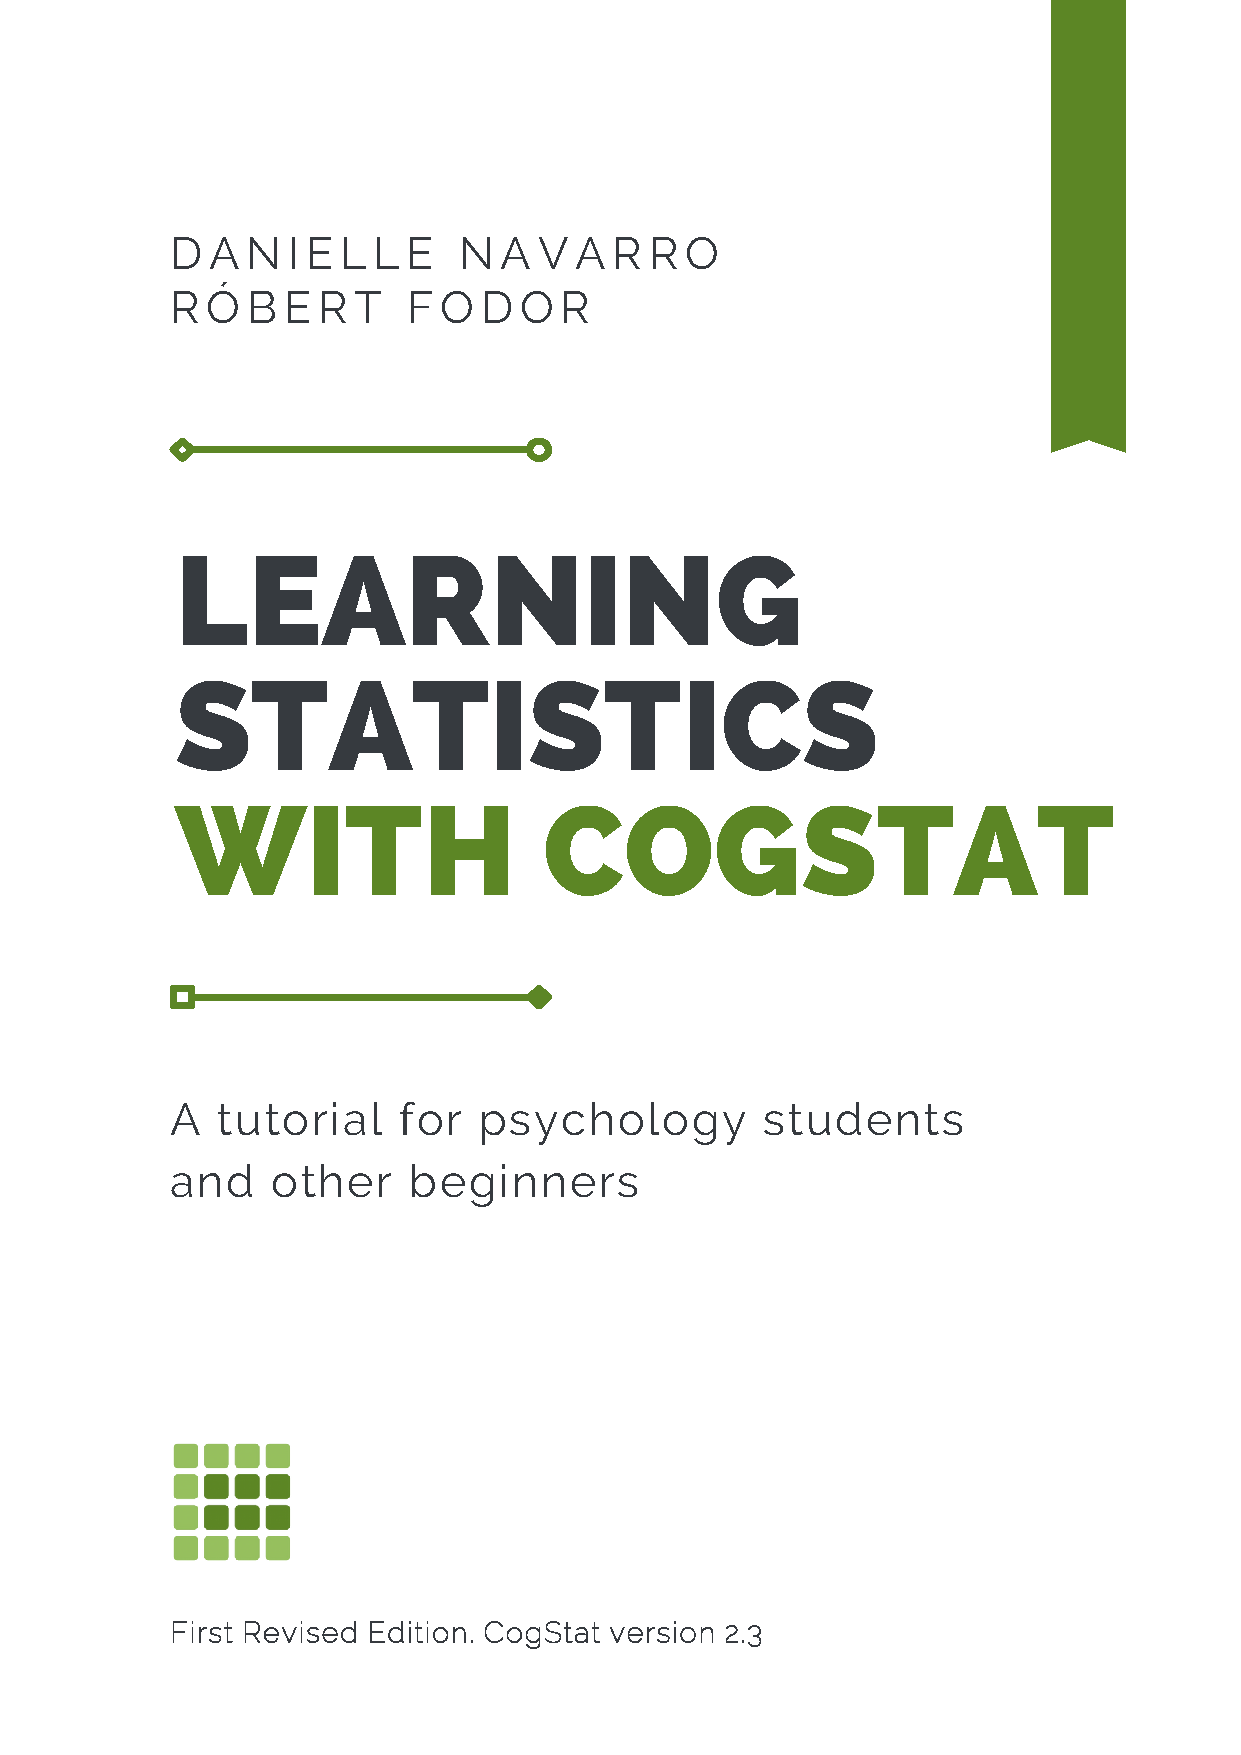
\includepdf[pages={1}, scale=1]{LSC_cover.pdf}
\newpage
    % This now makes the LaTeX title page after the cover page
\let\maketitle\oldmaketitle
\maketitle
\pagenumbering{roman} % This sets numbering to roman numerals
% Start numbering at 1
\setcounter{page}{1}

% This now sets numbering to arabic numerals
\mainmatter
\pagenumbering{arabic}

{
\hypersetup{linkcolor=black}
\setcounter{tocdepth}{1}
\tableofcontents
}
\hypertarget{about-this-book}{%
\chapter*{About this book}\label{about-this-book}}
\addcontentsline{toc}{chapter}{About this book}

\textbf{First revised edition} (v1.1 published XX January 2023)

Based on \textbf{Cogstat v2.3}

To reference this book, please use the following citation (APA7 format):

\begin{quote}
Navarro, D., \& Fodor, R. (2023). Learning Statistics with CogStat (Rev.~ed.).\\
\url{https://learningstatisticswithcogstat.com}
\end{quote}

\hypertarget{versions}{%
\section*{Versions}\label{versions}}
\addcontentsline{toc}{section}{Versions}

The online version of the book is updated regularly. The date of the last update is shown on the title page. The book features screenshots and result sets based on CogStat version 2.3.

\begin{itemize}
\tightlist
\item
  v1 \emph{First edition} was published on 27 September 2022 (electronic).
\item
  v1.0.1 Critical fixes applied (typos and minor errors) on 5 November 2022.
\item
  v1.1 \emph{First Revised Edition} was published on XX January 2023 (electronic).
\end{itemize}

\hypertarget{what-changed-in-v1.1-first-revised-edition}{%
\subsection*{\texorpdfstring{What changed in v1.1 \emph{First Revised Edition}?}{What changed in v1.1 First Revised Edition?}}\label{what-changed-in-v1.1-first-revised-edition}}
\addcontentsline{toc}{subsection}{What changed in v1.1 \emph{First Revised Edition}?}

\begin{itemize}
\tightlist
\item
  Chapters \ref{autostat} and \ref{cogstatintro} were amended and slightly expanded.
\item
  Chapter \ref{researchdesign} was largely revised to make explanations and examples more accurate.
\item
  Some paragraphs were rephrased or reordered to make them more clear in further chapters.
\item
  New: callout boxes added throughout the chapters to explain chart types and other concepts.
\item
  New: definitions and examples are now presented markedly in the text.
\item
  New: explanatory charts were added to the text.
\item
  Typos and minor errors were fixed all through the book.
\end{itemize}

Acknowledgements are due to Attila Krajcsi for his helpful notes as consulting editor for this version.

\hypertarget{authors-note}{%
\section*{Author's note}\label{authors-note}}
\addcontentsline{toc}{section}{Author's note}

This book is intended for psychology students and other beginners who are interested in learning statistics and want to use CogStat to perform their analyses. \href{https://www.cogstat.org}{CogStat} is a statistics software written in Python by Attila Krajcsi\footnote{Attila Krajcsi -- \href{http://www.attilakrajcsi.hu}{Website} \textbar{} \href{https://orcid.org/0000-0001-9792-9091}{
\includegraphics{resources/image/orcid_16x16.png}} 0000-0001-9792-9091} and developed with the help of supporters. Its distinct advantage is automatic hypothesis test selection and chart creation with an APA-style output to suit the needs of psychology researchers and students.

\emph{Learning Statistics with CogStat} is a book which covers the contents of an introductory statistics class. It is an adaptation made by Róbert Fodor based on Danielle Navarro's original \emph{(Learning Statistics with R)\footnote{\url{https://learningstatisticswithr.com}}} (Version 0.6\footnote{This book is compiled from scratch in bookdown but some code snippets rely on \href{https://twitter.com/emilyandthelime}{Emily Kothe}'s bookdown adaptation of the original material (e.g.~some knitr plots and tables appear in the source code without alteration), numbered as version \href{https://learningstatisticswithr.com/book/}{0.6.1}}). While the theory laid out in the original book is still valid, this book focuses on the practical application of statistical methods in CogStat. The book is not intended to be a comprehensive guide to either CogStat or statistical theory, though. One of the key challenges of the adaptation was to balance between a fully applied approach (like how CogStat handles analysis) and a theoretical one (like the fantastic textbook it is based on). Danielle's original content, while making up a massive chunk of the material, has been revised, reorganised, redacted, expanded on and rewritten to fit the new purpose.

This book will always be a living thing. As CogStat expands and evolves, so will this book. If you have any suggestions, comments or questions, please feel free to reach out to me on \href{https://github.com/robertfodor/lsc/issues}{GitHub}.

-- Robert

\hypertarget{licensing}{%
\section*{Licensing}\label{licensing}}

This book is published under a Creative Commons BY-SA license (CC BY-SA) version 4.0. This means that this book can be reused, remixed, retained, revised and redistributed (including commercially) as long as appropriate credit is given to the authors. If you remix, or modify the original version of this open textbook, you must redistribute all versions of this open textbook under the same license - CC BY-SA.

\url{https://creativecommons.org/licenses/by-sa/4.0/}

\hypertarget{part-introductions}{%
\part*{INTRODUCTIONS}\label{part-introductions}}
\addcontentsline{toc}{part}{INTRODUCTIONS}

\hypertarget{whywhywhy}{%
\chapter{Why do we learn statistics?}\label{whywhywhy}}

To the surprise of many students, statistics is a fairly significant part of a psychological education. To the surprise of no-one, statistics is very rarely the \emph{favourite} part of one's psychological education. Not surprisingly, there's a pretty large proportion of the student base that isn't happy about the fact that psychology has so much statistics in it. A big part of this issue at hand relates to the very idea of statistics.

\begin{quote}
\emph{Why do you do statistics? Why don't scientists just use \textbf{common sense?}}
\end{quote}

The best answer is a really simple one: we don't trust ourselves enough. We worry that we're human, and susceptible to all of the biases, temptations and frailties that humans suffer from. Much of statistics is basically a safeguard. Using ``common sense'' to evaluate evidence means trusting gut instincts, relying on verbal arguments and on using the raw power of human reason to come up with the right answer. Most scientists don't think this approach is likely to work.

\hypertarget{the-curse-of-belief-bias}{%
\section{The curse of belief bias}\label{the-curse-of-belief-bias}}

Our minds are quite amazing things, and we seem to be capable of the most incredible feats of thought and reason. Psychologists have shown over the years is that we really do find it hard to be neutral, to evaluate evidence impartially and without being swayed by pre-existing biases. A good example of this is the \textbf{\emph{belief bias effect}} in logical reasoning: if you ask people to decide whether a particular argument is logically valid (i.e., conclusion would be true if the premises were true), we tend to be influenced by the believability of the conclusion, even when we shouldn't. For instance, here's a valid argument where the conclusion is believable:

\begin{quote}
No cigarettes are inexpensive (Premise 1)\\
Some addictive things are inexpensive (Premise 2)\\
Therefore, some addictive things are not cigarettes (Conclusion)
\end{quote}

And here's a valid argument where the conclusion is not believable:

\begin{quote}
No addictive things are inexpensive (Premise 1)\\
Some cigarettes are inexpensive (Premise 2)\\
Therefore, some cigarettes are not addictive (Conclusion)
\end{quote}

The logical \emph{structure} of argument \#2 is identical to the structure of argument \#1, and they're both valid. However, in the second argument, there are good reasons to think that premise 1 is incorrect, and as a result it's probably the case that the conclusion is also incorrect. But that's entirely irrelevant to the topic at hand: an argument is deductively valid if the conclusion is a logical consequence of the premises. That is, a valid argument doesn't have to involve true statements.

On the other hand, here's an invalid argument that has a believable conclusion:

\begin{quote}
No addictive things are inexpensive (Premise 1)\\
Some cigarettes are inexpensive (Premise 2)\\
Therefore, some addictive things are not cigarettes (Conclusion)
\end{quote}

And finally, an invalid argument with an unbelievable conclusion:

\begin{quote}
No cigarettes are inexpensive (Premise 1)\\
Some addictive things are inexpensive (Premise 2)\\
Therefore, some cigarettes are not addictive (Conclusion)
\end{quote}

Now, suppose that people really are perfectly able to set aside their pre-existing biases about what is true and what isn't, and purely evaluate an argument on its logical merits. We'd expect 100\% of people to say that the valid arguments are valid, and 0\% of people to say that the invalid arguments are valid. So if you ran an experiment looking at this, you'd expect to see data like this:

\begin{table}[H]
\centering
\begin{tabular}{lcc}
\toprule
  & conclusion feels true & conclusion feels false\\
\midrule
argument is valid & 100\% say "valid" & 100\% say "valid"\\
argument is invalid & 0\% say "valid" & 0\% say "valid"\\
\bottomrule
\end{tabular}
\end{table}

If the psychological data looked like this (or even a good approximation to this), we might feel safe in just trusting our gut instincts. That is, it'd be perfectly okay just to let scientists evaluate data based on their common sense, and not bother with all this murky statistics stuff.

In a classic study, Evans et al. (\protect\hyperlink{ref-Evans1983}{1983}) ran an experiment looking at exactly this. What they found is that when pre-existing biases (i.e., beliefs) were in agreement with the structure of the data, everything went the way you'd hope:

\begin{table}[H]
\centering
\begin{tabular}{lcc}
\toprule
  & conclusion feels true & conclusion feels false\\
\midrule
argument is valid & 92\% say "valid" & \\
argument is invalid &  & 8\% say "valid"\\
\bottomrule
\end{tabular}
\end{table}

Not perfect, but that's pretty good. But look what happens when our intuitive feelings about the truth of the conclusion run against the logical structure of the argument:

\begin{table}[H]
\centering
\begin{tabular}{lcc}
\toprule
  & conclusion feels true & conclusion feels false\\
\midrule
argument is valid & 92\% say "valid" & **46\% say "valid"**\\
argument is invalid & **92\% say "valid"** & 8\% say "valid"\\
\bottomrule
\end{tabular}
\end{table}

Apparently, when people are presented with a strong argument that contradicts our pre-existing beliefs, we find it pretty hard to even perceive it to be a strong argument (people only did so 46\% of the time). Even worse, when people are presented with a weak argument that agrees with our pre-existing biases, almost no-one can see that the argument is weak.

It's just \emph{too easy} for us to ``believe what we want to believe''; so if we want to ``believe in the data'' instead, we're going to need a bit of help to keep our personal biases under control. That's what statistics does: it helps keep us honest.

\hypertarget{the-simpsons-paradox}{%
\section{The Simpson's paradox}\label{the-simpsons-paradox}}

In 1973, the University of California, Berkeley had some worries about the admissions of students into their postgraduate courses. Specifically, the thing that caused the problem was that the gender breakdown of their admissions, which looked like this:

\begin{table}[H]
\centering
\begin{tabular}{lcc}
\toprule
  & Number of applicants & Percent admitted\\
\midrule
Males & 8442 & 46\%\\
Females & 4321 & 35\%\\
\bottomrule
\end{tabular}
\end{table}

Given that there were nearly 13,000 applicants, a difference of 9\% in admission rates between males and females is just way too big to be a coincidence. When people started looking more carefully at the admissions data (\protect\hyperlink{ref-Bickel1975}{Bickel et al., 1975}) on a department by department basis, it turned out that most of the departments actually had a slightly \emph{higher} success rate for female applicants than for male applicants. Table \ref{tab:simpsontable} shows the admission figures for the six largest departments:

\begin{table}[H]

\caption{\label{tab:simpsontable}Admission figures for the six largest departments by gender}
\centering
\resizebox{\linewidth}{!}{
\begin{tabular}[t]{lcclc}
\toprule
Department & Male Applicants & Male Percent Admitted & Female Applicants & Female Percent admitted\\
\midrule
A & 825 & 62\% & 108 & 82\%\\
B & 560 & 63\% & 25 & 68\%\\
C & 325 & 37\% & 593 & 34\%\\
D & 417 & 33\% & 375 & 35\%\\
E & 191 & 28\% & 393 & 24\%\\
F & 272 & 6\% & 341 & 7\%\\
\bottomrule
\end{tabular}}
\end{table}

Remarkably, most departments had a \emph{higher} rate of admissions for females than for males! Yet the overall rate of admission across the university for females was \emph{lower} than for males. How can this be? How can both of these statements be true at the same time?

Here's what's going on. Firstly, notice that the departments are \emph{not} equal to one another in terms of their admission percentages: some departments (e.g., engineering, chemistry) tended to admit a high percentage of the qualified applicants, whereas others (e.g., English) tended to reject most of the candidates, even if they were high quality. So, among the six departments shown above, notice that department A is the most generous, followed by B, C, D, E and F in that order. Next, notice that males and females tended to apply to different departments. If we rank the departments in terms of the total number of male applicants, we get \textbf{A}\textgreater{}\textbf{B}\textgreater D\textgreater C\textgreater F\textgreater E (the ``easy'' departments are in bold). On the whole, males tended to apply to the departments that had high admission rates. Now compare this to how the female applicants distributed themselves. Ranking the departments in terms of the total number of female applicants produces a quite different ordering C\textgreater E\textgreater D\textgreater F\textgreater{}\textbf{A}\textgreater{}\textbf{B}.

In other words, what these data seem to be suggesting is that the female applicants tended to apply to ``harder'' departments. And in fact, if we look at all Figure \ref{fig:berkeley} we see that this trend is systematic, and quite striking. This effect is known as Simpson's paradox. It's not common, but it does happen in real life, and most people are very surprised by it when they first encounter it, and many people refuse to even believe that it's real. It is very real.

When doing research, there are \emph{lots} of subtle, counterintuitive traps lying in wait for the unwary. Truth is sometimes cunningly hidden in the nooks and crannies of complicated data.



\begin{figure}

{\centering 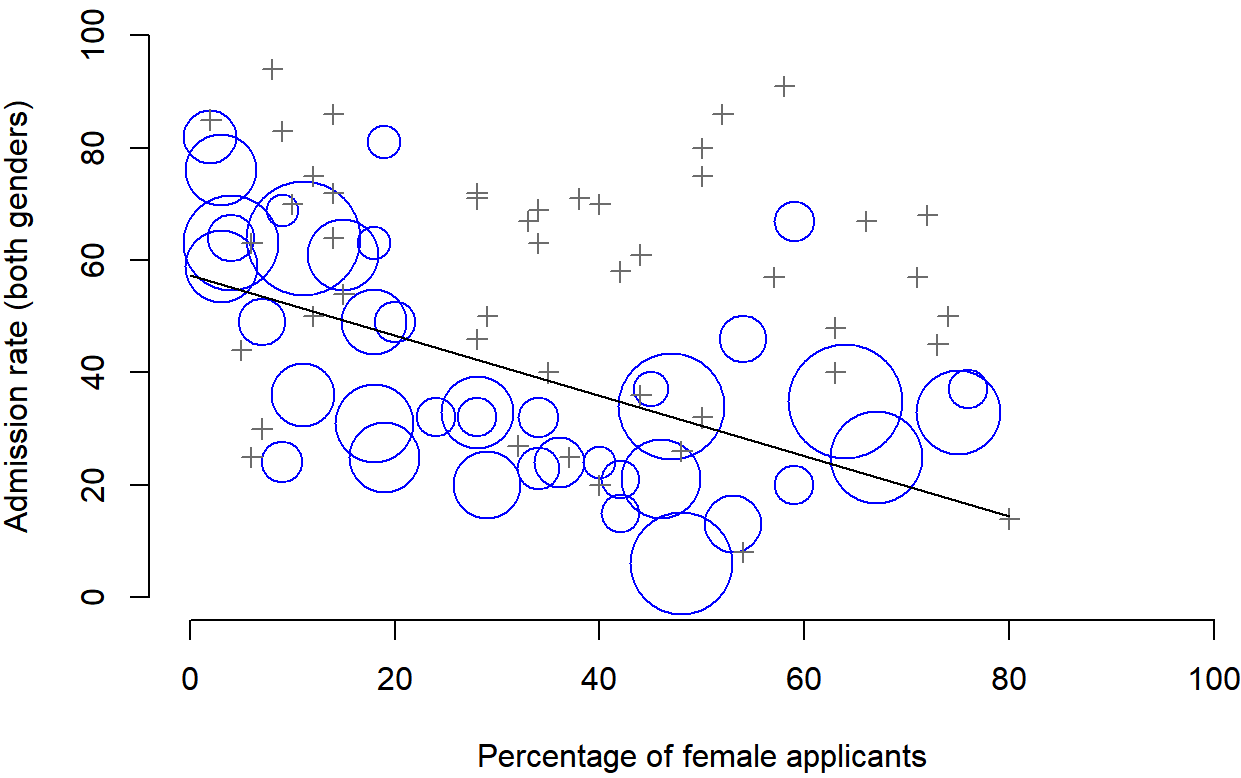
\includegraphics[width=0.66\linewidth]{resources/image/berkeley} 

}

\caption[The Berkeley 1973 college admissions data.]{The Berkeley 1973 college admissions data. This figure plots the admission rate for the 85 departments that had at least one female applicant, as a function of the percentage of applicants that were female. The plot is a redrawing of Figure 1 from (\protect\hyperlink{ref-Bickel1975}{Bickel et al., 1975}). Circles plot departments with more than 40 applicants; the area of the circle is proportional to the total number of applicants. The crosses plot department with fewer than 40 applicants.}\label{fig:berkeley}
\end{figure}

Statistics only solves \emph{part} of the problem. Remember that we started all this with the concern that Berkeley's admissions processes might be unfairly biased against female applicants. When we looked at the ``aggregated'' data, it did seem like the university was discriminating against women, but when we ``disaggregate'' and looked at the individual behaviour of all the departments, it turned out that the actual departments were, if anything, slightly biased in favour of women. The gender bias in total admissions was caused by the fact that women tended to self-select for harder departments. Postgraduate admissions are determined at the level of the individual department (and there are good reasons to do that), and at the level of individual departments, the decisions are more or less unbiased (the weak bias in favour of females at that level is small, and not consistent across departments). Since the university can't dictate which departments people choose to apply to, and the decision making takes place at the level of the department it can hardly be held accountable for any biases that those choices produce.

If we're interested in this from a more sociological and psychological perspective, we might want to ask \emph{why} there are such strong gender differences in applications. Why do males tend to apply to engineering more often than females, and why is this reversed for the English department? And why is it it the case that the departments that tend to have a female-application bias tend to have lower overall admission rates than those departments that have a male-application bias? Might this not still reflect a gender bias, even though every single department is itself unbiased? It might. Suppose, hypothetically, that males preferred to apply to ``hard sciences'' and females prefer ``humanities''. And suppose further that the reason for why the humanities departments have low admission rates is because the government doesn't want to fund the humanities (Ph.D.~places, for instance, are often tied to government funded research projects). Does that constitute a gender bias? Or just an unenlightened view of the value of the humanities? What if someone at a high level in the government cut the humanities funds because they felt that the humanities are ``useless chick stuff''. That seems pretty \emph{blatantly} gender biased. None of this falls within the purview of statistics, but it matters to the research project. If you're interested in the overall structural effects of subtle gender biases, then you probably want to look at \emph{both} the aggregated and disaggregated data. If you're interested in the decision making process at Berkeley itself then you're probably only interested in the disaggregated data.

In short there are a lot of critical questions that you can't answer with statistics, but the answers to those questions will have a huge impact on how you analyse and interpret data. And this is the reason why you should always think of statistics as a \emph{tool} to help you learn about your data, no more and no less. It's a powerful tool to that end, but there's no substitute for careful thought.

\hypertarget{statistics-in-psychology}{%
\section{Statistics in psychology}\label{statistics-in-psychology}}

We hope that the discussion above helped explain why science in general is so focused on statistics. But we're guessing that you have a lot more questions about what role statistics plays in psychology, and specifically why psychology classes always devote so many lectures to stats. So here's an attempt to answer a few of them\ldots{}

\textbf{Why does psychology have so much statistics?}

The most important reason is that psychology is a statistical science. There's a saying used sometimes in physics, to the effect that ``if your experiment needs statistics, you should have done a better experiment''.

The ``things'' that we study are \emph{people}. Real, complicated, gloriously messy people. The ``things'' of physics include object like electrons, and while there are all sorts of complexities that arise in physics, electrons don't have minds of their own. They don't have opinions, they don't differ from each other in weird and arbitrary ways, they don't get bored in the middle of an experiment, and they don't get angry at the experimenter and then deliberately try to sabotage the data set.\footnote{Some may argue that natural science experiments still struggle with data quality, noise etc. But to the best of my knowledge, there's no evidence of electron producing response bias in the lab due to over- or undercompliance. -- Robert}

We teach statistics to you as psychologists because you need to be better at stats than physicists. They have the luxury of being able to say that because their objects of study are simple in comparison to the vast mess that confronts social scientists.

\textbf{Can't someone else do the statistics?}

To some extent, but not completely. It's true that you don't need to become a fully trained statistician just to do psychology, but you do need to reach a certain level of statistical competence. There's three reasons that every psychological researcher ought to be able to do basic statistics:

\begin{itemize}
\tightlist
\item
  Firstly, there's the fundamental reason: statistics is deeply intertwined with research design. If you want to be good at designing psychological studies, you need to at least understand the basics of stats.
\item
  Secondly, if you want to be good at the psychological side of the research, then you need to be able to understand the psychological literature, right? But almost every paper in the psychological literature reports the results of statistical analyses. So if you really want to understand the psychology, you need to be able to understand what other people did with their data. And that means understanding a certain amount of statistics.
\item
  Thirdly, there's a big practical problem with being dependent on other people to do all your statistics: statistical analysis is \emph{expensive}. In almost any real life situation where you want to do psychological research, the cruel facts will be that you don't have enough money to afford a statistician. So the economics of the situation mean that you have to be self-sufficient.
\end{itemize}

Note that a lot of these reasons generalise beyond researchers. If you want to be a practicing psychologist and stay on top of the field, it helps to be able to read the scientific literature, which relies pretty heavily on statistics.

\textbf{I don't care about jobs, research, or clinical work. Do I need statistics?}

Statistics should matter to you in the same way that statistics should matter to \emph{everyone}: we live in the 21st century, and data are \emph{everywhere}. Frankly, given the world in which we live these days, a basic knowledge of statistics is pretty damn close to a survival tool! Which is the topic of the next section\ldots{}

\hypertarget{theres-more-to-research-methods-than-statistics}{%
\section{There's more to research methods than statistics}\label{theres-more-to-research-methods-than-statistics}}

Most research methods courses will cover a lot of topics that relate much more to the pragmatics of research design, and in particular the issues that you encounter when trying to do research with humans. Most student fears relate to the statistics part of the course. Hopefully you are convinced that statistics matters, and more importantly, that it's not to be feared.

Introductory classes focus a lot on the statistics because you almost always find yourself needing statistics before you need the other research methods training. Why? Because almost all of your assignments in other classes will rely on statistical training, to a much greater extent than they rely on other methodological tools. It's not common for undergraduate assignments to require you to design your own study from the ground up (in which case you would need to know a lot about research design), but it is common for assignments to ask you to analyse and interpret data that were collected in a study that someone else designed (in which case you need statistics). In that sense, from the perspective of allowing you to do well in all your other classes, the statistics is more urgent.

But note that ``urgent'' is different from ``important'' -- they both matter. We really do want to stress that research design is just as important as data analysis, and this book does spend a fair amount of time on it. However, while statistics has a kind of universality, and provides a set of core tools that are useful for most types of psychological research, the research methods side isn't quite so universal. There are some general principles that everyone should think about, but a lot of research design is very idiosyncratic, and is specific to the area of research that you want to engage in. To the extent that it's the details that matter, those details don't usually show up in an introductory stats and research methods class.

\hypertarget{autostat}{%
\chapter{An introduction to automatic statistical analysis}\label{autostat}}

In recent years, the reliability of psychological science has been questioned due to the overstated use of \(p\)-values and effect sizes, and their lower-than-expected replicability (\protect\hyperlink{ref-open_science_collaboration_estimating_2015}{Open Science Collaboration, 2015}). This may be a result of the high pressure on researchers to produce a large volume of work with statistically positive results (\protect\hyperlink{ref-krajcsi_advancing_2021}{Krajcsi, 2021}).

To produce strong research results, it is important to have good data analysis, which can make or break a research project. In psychological research, this includes: identifying and selecting a good design from many alternative design options, sampling participants appropriately, observing ethical standards in data collection and documentation, controlling for confounding variables, selecting appropriate statistics and replications of analyses, analysing data with appropriate software, assessing the effect sizes of results based on their inferential characteristics, reporting findings accurately in papers -- just to name a few. Some of these tasks can be automated to ensure that the appropriate protocol is followed, which is why we have CogStat, and why you are reading this book.

Neglecting early protocols can lead to errors. For example, using a tool designed for \emph{normally distributed} data on a highly \emph{skewed} data set will be inappropriate. In this book, we will cover why this characteristic of our data set matters. Ignoring the foundations of hypothesis testing tools will harm the reliability of the research and, in turn, the reliability and prestige of psychology as a science.

There are several manual statistical programs, such as SPSS, SAS, and Stata, and some programming languages used for data analysis, such as R and Python. These tools can be time-consuming and require multiple steps for simple tasks like creating tables and graphs, not to mention the time spent on learning how to use them. One benefit of automatic statistical software is that it is programmed to follow all necessary steps as part of its protocol. A good automatic statistical software will apply the most appropriate tools based on current statistical consensus.

In this book, you will learn what it means to do normality and heteroscedasticity checks, calculate effect sizes, and performing hypothesis tests etc. We focus on making sure you understand what they are, why they matter, and how to interpret them. We will indulge in presenting mathematical formulas as well, but you won't have to do any of the calculations. To be fair, you don't have to manually calculate the respective metrics in a manual statistical program either, but deciding which tool to pick up first, or which step to take next might be a challenge if statistics is not in your veins. Beyond the anxiety of how to even get started with manual statistical programs, applying a single tool can take up to tens of steps. In comparison, producing the full analysis with multiple tools with supporting charts and graphs may only take three steps in CogStat.

Researchers often have too little time for rigorous data analysis and interpretation, and at the same time, journals set somewhat arbitrary standards (e.g.~specific \(p\)-values are demanded whether or not they avoid Type I errors -- this is one of the topics in this book), so some researchers might just use those as rules of thumb without going deeper into data analysis. By using an automatic procedure, the time spent on data analysis can be redirected towards understanding the implications of the test results for the research question.

For more about the merits of automatic statistical analysis, here are some further reads from Attila Krajcsi, the creator of CogStat:

\begin{itemize}
\tightlist
\item
  \href{https://psyarxiv.com/hnmsq}{Methodological considerations behind CogStat}
\item
  \href{https://docs.google.com/presentation/d/1HmSTPnTxDzW8hYZG7ujHaeHc0mRqqYeY95yKh56z61c}{Reducing the replication crisis}
\end{itemize}

\hypertarget{cogstatintro}{%
\chapter{An Introduction to CogStat}\label{cogstatintro}}

CogStat is a statistical analysis program designed for psychology research, particularly in cognitive science. It is user-friendly and automatic, yet powerful enough to handle a variety of statistical analyses. CogStat is free to download from the \href{http://cogstat.org}{CogStat website} and runs on Windows, macOS, and Linux.

The main feature of CogStat is its automatic analysis of source data and automatic selection of hypothesis tests, which can be very useful after learning about statistical theory and hypothesis testing. The program will automatically choose the most appropriate statistical test for your data, making it a useful tool for researchers who want to save time on test selection or are unsure of the best fit for their purposes.

CogStat automatically analyzes data based on its scale type, runs necessary pre-checks (such as for normality and heteroscedasticity), and performs the appropriate hypothesis test. The results are presented in a clear format following APA7 guidelines, and the program also generates graphical representations of the results.

To install CogStat, simply download the latest version from the \href{http://cogstat.org}{CogStat website}. The installation is easy and straightforward, and should only take a few minutes. For help with installation, please visit our \href{https://github.com/cogstat/cogstat/wiki/Installation}{GitHub page}.

To quickly test CogStat without using your own data, you can use the demo data provided in the program. From the \texttt{Data\ \textgreater{}\ Open\ demo\ data\ file...} menu, choose a folder and data file, then click \texttt{Open}.

To use your own data with CogStat, prepare it in spreadsheet software like Excel, Google Spreadsheet, or LibreOffice Calc, or in statistical software like jamovi, JASP, SPSS, STATA, or SAS. CogStat does not handle data editing tasks, as there are more efficient solutions available. To import your data into CogStat, you can either copy and paste it from your spreadsheet software, or import it as a saved file (.xlsx, .ods, .csv, .jasp, .omv, .rdata etc.). You can also drag and drop the file into the CogStat window.

If your data comes from a spreadsheet software or is a text file, like .csv, make sure of the following:

\begin{itemize}
\tightlist
\item
  The first row of your data should include the variable names without accent characters (áâő\ldots).
\item
  The second row should include the measurement levels: \texttt{int} for interval and ratio scales, \texttt{ord} for ordinal variables, and \texttt{nom} for nominal variables. More on measurement levels (scales) in Chapter \ref{scales}. The remaining rows should include the values of the variables.
\end{itemize}

To learn more about using CogStat, including how to prepare and load data, refer to the \href{https://github.com/cogstat/cogstat/wiki/Documentation-for-users}{GitHub Wiki page}.

\hypertarget{researchdesign}{%
\chapter{A brief introduction to research design}\label{researchdesign}}

In this chapter, we'll start thinking about the basic ideas for designing a study, collecting data, checking whether your data collection works, and so on. It won't give you enough information to design studies of your own, but it will provide you with a lot of the essential tools you need to assess the studies done by other people. Since this book focuses more on data analysis than data collection, this only gives a very brief overview. This chapter relies heavily on Campbell \& Stanley (\protect\hyperlink{ref-Campbell1963}{1963}) for discussing study design and Stevens (\protect\hyperlink{ref-Stevens1946}{1946}) for discussing scales of measurement.

\hypertarget{measurement}{%
\section{Introduction to psychological measurement}\label{measurement}}

First, data collection can be thought of as a kind of \textbf{\emph{measurement}}. That is, what we're trying to do here is measure something about human behaviour or the human mind. What do we mean by ``measurement''?

\hypertarget{some-thoughts-about-psychological-measurement}{%
\subsection{Some thoughts about psychological measurement}\label{some-thoughts-about-psychological-measurement}}

Measurement itself is a subtle concept, but it comes down to finding some way of assigning numbers, labels, or other well-defined descriptions to ``stuff''. So, any of the following would count as a psychological measurement:

\begin{itemize}
\tightlist
\item
  Danielle's \textbf{age} is \emph{33 years}.
\item
  She \emph{does not} \textbf{like anchovies}.
\item
  Her \textbf{chromosomal gender} is \emph{male}.
\item
  Her \textbf{self-identified gender} is \emph{female}.
\end{itemize}

In the short list above, the \textbf{bolded part} is ``the thing to be measured'', and the \emph{italicised part} is ``the measurement itself''. We can expand on this a little bit by thinking about the set of possible measurements that could have arisen in each case:

\begin{itemize}
\tightlist
\item
  \textbf{Age} (in years) could have been \emph{0, 1, 2, 3 \ldots{}}, etc. The upper bound on what the age could be is a bit fuzzy, but in practice, you'd be safe in saying that the largest possible age is \emph{150} since no human has ever lived that long.
\item
  When asked if someone \textbf{likes anchovies}, they might say \emph{I do}, \emph{I do not}, \emph{I have no opinion}, or \emph{I sometimes do}.
\item
  \textbf{Chromosomal gender} is almost certainly going to be \emph{male (XY)} or \emph{female (XX)}, but there are a few other possibilities: with \emph{Klinefelter's syndrome (XXY)}, it is more similar to male than to female. And there are other possibilities, too.
\item
  \textbf{Self-identified gender} is also very likely to be \emph{male} or \emph{female}, \emph{transgender}, \emph{nonbinary}, \emph{queer} etc.
\end{itemize}

As you can see, for some things (like age), it seems pretty apparent what the set of possible measurements should be, whereas, for other things, it gets a bit tricky. But even regarding someone's age, it's much more subtle than this. For instance, if you're a developmental psychologist, measuring in \emph{years} is way too crude, and so you often measure age in \emph{years and months} (if a child is 2 years and 11 months, this is usually written as ``2;11''). If you're interested in newborns, you might want to measure age in \emph{days since birth}, or maybe even \emph{hours since birth}.

Looking at this a bit more closely, you might also realise that the concept of ``age'' isn't all that precise. Generally, when we say ``age'', we implicitly mean ``the length of time since birth''. But that's not always the right way to do it. Suppose you're interested in how newborn babies control their eye movements. If you're interested in kids that young, you might also start to worry that ``birth'' is not the only significant point in time to care about. If Baby Alice is born 3 weeks premature and Baby Bianca is born 1 week late, would it really make sense to say that they are the ``same age'' if we encountered them ``2 hours after birth''? In a sense, yes. By social convention, we use birth as our reference point for talking about age in everyday life since it defines the amount of time the person has been operating as an independent entity in the world. But from a scientific perspective, that's not the only thing we care about. When we think about the biology of human beings, it's often helpful to think of ourselves as organisms that have been growing and maturing since conception. From that perspective, Alice and Bianca aren't the same age at all. So you might want to define the concept of ``age'' in two different ways: the length of time since conception and the length of time since birth. It won't make much difference when dealing with adults, but when dealing with newborns, it might.

In other words, how you specify the allowable measurement values is important.

Still, there's the question of methodology. What specific ``measurement method'' will you use to find out someone's age? As before, there are lots of different possibilities:

\begin{itemize}
\tightlist
\item
  You could just ask people, ``how old are you?'' The method of self-report is fast, cheap and easy, but it only works with people old enough to understand the question, and some people lie about their age.
\item
  You could ask an authority (e.g.~a parent), ``how old is your child?'' This method is fast, and it's not all that hard when dealing with kids since the parent is almost always around. It doesn't work as well if you want to know ``age since conception'' since a lot of parents can't say for sure when conception took place. You might need a different authority (e.g.~an obstetrician).
\item
  You could look up official records, like birth certificates. This is time-consuming and annoying, but it has its uses (e.g.~if the person is now dead).
\end{itemize}

\hypertarget{operationalisation-defining-your-measurement}{%
\subsection{Operationalisation: defining your measurement}\label{operationalisation-defining-your-measurement}}

All of the ideas discussed in the previous section relate to the concept of \textbf{operationalisation}. To be a bit more precise about the idea, operationalisation is the process by which we take a meaningful but somewhat vague concept and turn it into an accurate measurement. The method of operationalisation can involve several different things:

\begin{itemize}
\tightlist
\item
  Being precise about what you are trying to measure. For instance, does ``age'' mean ``time since birth'' or ``time since conception'' in the context of your research?
\item
  Determining what method you will use to measure it. Will you use self-report to measure age, ask a parent, or look up an official record? If you're using self-report, how will you phrase the question?
\item
  Defining the set of allowable values that the measurement can take. Note that these values don't always have to be numerical, though they often are. When measuring age, the values are numerical, but we still need to think carefully about what numbers are allowed. Do we want age in years, years and months, days, or hours? The values aren't numerical for other types of measurements (e.g.~gender). But, as before, we need to consider what values are allowed. If we're asking people to self-report their gender, what options do we allow them to choose from? Is it enough to allow only ``male'' or ``female''? Do you need an ``other'' option? Or should we not give people any specific options and let them answer in their own words? And if you open up the set of possible values to include all verbal responses, how will you interpret their answers?
\end{itemize}

Operationalisation is tricky, and there's no ``one, true way'' to do it. How you operationalise the informal concept of ``age'' or ``gender'' into a formal measurement depends on what you need to use the measurement for. You'll often find that the community of scientists who work in your area have some well-established ideas for how to go about it. In other words, operationalisation needs to be thought through case-by-case. Nevertheless, while there are a lot of issues that are specific to each individual research project, there are some aspects to it that are pretty general.

Before moving on, let's take a moment to clear up our terminology and, in the process, introduce one more term. Here are four different things that are closely related to each other:

\begin{itemize}
\tightlist
\item
  \textbf{\emph{A theoretical construct}}. This is the thing that you're trying to measure, like ``age'', ``gender'', or an ``opinion''. A theoretical construct can't be directly observed, and often they're a bit vague.
\item
  \textbf{\emph{A measure}}. The measure refers to the method or tool used to make your observations. A question in a survey, a behavioural observation or a brain scan could all count as a measure.
\item
  \textbf{\emph{An operationalisation}}. The term ``operationalisation'' refers to the logical connection between the measure and the theoretical construct or the process by which we try to derive a measure from a theoretical construct.
\item
  \textbf{\emph{A variable}}. Finally, a new term. A variable is what we end up with when we apply our measure to something in the world. That is, variables are the actual ``data'' we end up with in our data sets.
\end{itemize}

In practice, even scientists tend to blur the distinction between these things, but it's very helpful to understand the differences.

\hypertarget{scales}{%
\section{Scales of measurement (measurement levels)}\label{scales}}

As the previous section indicates, the outcome of a psychological measurement is called a variable. But not all variables are of the same qualitative type, and it's handy to understand what types there are. A very useful concept for distinguishing between different types of variables is what's known as \textbf{\emph{scales of measurement}}, or in CogStat terminology, \textbf{\emph{measurement levels}}.

\hypertarget{nominalscale}{%
\subsection{Nominal scale}\label{nominalscale}}

A \textbf{nominal scale} variable (also referred to as a \textbf{categorical} variable) is one in which there is no particular relationship between the different possibilities: for these kinds of variables, it doesn't make any sense to say that one of them is ``bigger' or''better'' than any other one, and it doesn't make any sense to average them. The classic example for this is ``eye colour''. Eyes can be blue, green and brown, among other possibilities, but none of them is any ``better'' than any other one. As a result, it would feel bizarre to talk about an ``average eye colour''. Similarly, gender is nominal too: \emph{male} isn't better or worse than \emph{female}, neither does it make sense to try to talk about an ``average gender''. In short, nominal scale variables are those for which the only thing you can say about the different possibilities is that they are different. That's it.

Let's take a slightly closer look at this. Suppose we were researching how people commute to and from work. One variable we would have to measure would be what kind of transportation people use to get to work. This ``transport type'' variable could have quite a few possible values, including: ``train'', ``bus'', ``car'', ``bicycle'', etc. For now, let's suppose that these four are the only possibilities, and suppose that when we ask 100 people how they got to work today, we get this:

\begin{table}[H]
\centering
\begin{tabular}{lc}
\toprule
Transportation & Number of people\\
\midrule
(1) Train & 12\\
(2) Bus & 30\\
(3) Car & 48\\
(4) Bicycle & 10\\
\bottomrule
\end{tabular}
\end{table}

So, what's the average transportation type? Obviously, the answer here is that there isn't one. It's a silly question to ask. You can say that travel by car is the most popular method, and travel by train is the least popular method, but that's about all. Similarly, notice that the order in which the options are listed isn't very exciting. We could have chosen to display the data like this:

\begin{table}[H]
\centering
\begin{tabular}{lc}
\toprule
Transportation & Number of people\\
\midrule
(3) Car & 48\\
(1) Train & 12\\
(4) Bicycle & 10\\
(2) Bus & 30\\
\bottomrule
\end{tabular}
\end{table}

-- and nothing really changes.

\hypertarget{ordinalscale}{%
\subsection{Ordinal scale}\label{ordinalscale}}

\textbf{Ordinal scale} variables have a bit more structure than nominal scale variables, but not by a lot. An ordinal scale variable is one in which there is a natural, meaningful way to order the different possibilities, but you can't do anything else. The usual example of an ordinal variable is ``finishing position in a race''. You \emph{can} say that the person who finished first was faster than the person who finished second, but you \emph{don't} know how much faster. Consequently, we know that 1st \textgreater{} 2nd, and 2nd \textgreater{} 3rd, but the difference between 1st and 2nd might be much larger than the difference between 2nd and 3rd.

Here's a more psychologically exciting example. Suppose we're interested in people's attitudes to climate change, and we ask them to pick one of these four statements that most closely matches their beliefs:

\begin{quote}
\begin{enumerate}
\def\labelenumi{(\arabic{enumi})}
\tightlist
\item
  Temperatures are rising because of human activity
\item
  Temperatures are rising, but we don't know why
\item
  Temperatures are rising, but not because of humans
\item
  Temperatures are not rising
\end{enumerate}
\end{quote}

Notice that these four statements actually do have a natural ordering in terms of ``the extent to which they agree with the current science''. Statement 1 is a close match, statement 2 is a suitable match, statement 3 isn't a perfect match, and statement 4 strongly opposes science. So, in terms of the thing we're interested in (the extent to which people endorse the science), we can order the items as 1 \textgreater{} 2 \textgreater{} 3 \textgreater{} 4. Since this ordering exists, it would be peculiar to list the options like this:

\begin{quote}
\begin{enumerate}
\def\labelenumi{(\arabic{enumi})}
\setcounter{enumi}{2}
\tightlist
\item
  Temperatures are rising, but not because of humans
\item
  Temperatures are rising because of human activity
\item
  Temperatures are not rising
\item
  Temperatures are rising, but we don't know why
  -- because it seems to violate the natural ``structure'' of the question.
\end{enumerate}
\end{quote}

So, let's suppose I asked 100 people these questions and got the following answers:

\begin{table}[H]
\centering
\begin{tabular}{lc}
\toprule
Response & Number\\
\midrule
(1) Temperatures are rising because of human activity & 51\\
(2) Temperatures are rising, but we don't know why & 20\\
(3) Temperatures are rising, but not because of humans & 10\\
(4) Temperatures are not rising & 19\\
\bottomrule
\end{tabular}
\end{table}

When analysing these data, it seems quite reasonable to try to group (1), (2) and (3) together and say that 81 of 100 people were willing to \emph{at least partially} endorse the science. And it's \emph{also} quite reasonable to group (2), (3) and (4) together and say that 49 of 100 people registered \emph{at least some disagreement} with the dominant scientific view. However, it would be entirely bizarre to try to group (1), (2) and (4) together and say that 90 of 100 people said what? There's nothing sensible that allows you to group those responses together at all.

That said, notice that while we \emph{can} use the natural ordering of these items to construct sensible groupings, what we \emph{can't} do is average them. For instance, in our simple example here, the ``average'' response to the question is 1.97. We would love to know if someone can tell us what that means.

\hypertarget{intervalscale}{%
\subsection{Interval scale}\label{intervalscale}}

In contrast to nominal and ordinal scale variables, \textbf{interval scale} and ratio scale variables are variables for which the numerical value is genuinely meaningful. In the case of interval scale variables, the \emph{differences} between the numbers are interpretable, but the variable doesn't have a ``natural'' zero value. A good example of an interval scale variable is measuring temperature in degrees Celsius. For instance, if it was 15\(^\circ\) yesterday and 18\(^\circ\) today, then the 3\(^\circ\) difference between the two is genuinely meaningful. Moreover, that 3\(^\circ\) difference is \emph{exactly the same} as the 3\(^\circ\) difference between 7\(^\circ\) and 10\(^\circ\). In short, addition and subtraction are meaningful for interval scale variables.\footnote{Actually, temperature isn't strictly an interval scale, in the sense that the amount of energy required to heat something up by 3\(^\circ\) depends on its current temperature. So in the sense that physicists care about, temperature isn't actually an interval scale.}

However, notice that the 0\(^\circ\) does not mean ``no temperature at all'': it means ``the temperature at which water freezes'', which is pretty arbitrary. As a consequence, it becomes pointless to try to multiply and divide temperatures. It is wrong to say that \(20^\circ\) is \emph{twice as hot} as 10\(^\circ\), just as it is weird and meaningless to claim that 20\(^\circ\) is negative two times as hot as -10\(^\circ\).

Again, let us look at a more psychological example. Suppose we're interested in looking at how the attitudes of first-year university students have changed over time. We will want to record the year in which each student started. This is an interval scale variable. A student who started in 2003 did arrive 5 years before a student who started in 2008. However, it would be completely insane for me to divide 2008 by 2003 and say that the second student started ``1.0024 times later'' than the first one. That doesn't make any sense at all.

\hypertarget{ratioscale}{%
\subsection{Ratio scale}\label{ratioscale}}

The fourth and final type of variable to consider is a \textbf{ratio scale} variable, in which zero really means zero, and it's okay to multiply and divide. A good psychological example of a ratio scale variable is response time (RT). In many tasks, it's very common to record the amount of time somebody takes to solve a problem or answer a question because it's an indicator of how difficult the task is. Suppose that Alan takes 2.3 seconds to respond to a question, whereas Ben takes 3.1 seconds. As with an interval scale variable, addition and subtraction are both meaningful here. Ben really did take 3.1 - 2.3 = 0.8 seconds longer than Alan did. However, notice that multiplication and division also make sense here: Ben took 3.1 / 2.3 = 1.35 times as long as Alan did to answer the question. And you can do this because, for a ratio scale variable such as RT, ``zero seconds'' really means ``no time at all''.

\hypertarget{continuousdiscrete}{%
\subsection{Continuous versus discrete variables}\label{continuousdiscrete}}

There's a second kind of distinction that you need to be aware of regarding what types of variables you can run into. This is the distinction between continuous variables and discrete variables. The difference between these is as follows:

\begin{itemize}
\tightlist
\item
  A \textbf{continuous variable} is one in which, for any two values you can think of, it's always logically possible to have another value in between.
\item
  A \textbf{discrete variable} is, in effect, a variable that isn't continuous. For a discrete variable, it's sometimes the case that there's nothing in the middle.
\end{itemize}

These definitions probably seem a bit abstract, but they're pretty simple once you see some examples. For instance, response time is continuous. If Alan takes 3.1 seconds and Ben takes 2.3 seconds to respond to a question, then Cameron's response time can lie in between by taking 3.0 seconds. And, of course, it would also be possible for David to take 3.031 seconds to respond, meaning that his RT would lie in between Cameron's and Alan's. And while in practice, it might be impossible to measure RT that precisely, it's certainly possible in principle. Because we can always find a new value for RT in between any two other ones, we say that RT is continuous.

Discrete variables occur when this rule is violated. For example, nominal scale variables are always discrete: there isn't a type of transportation that falls ``in-between'' trains and bicycles, not in the strict mathematical way that 2.3 falls in between 2 and 3. So transportation type is discrete. Similarly, ordinal scale variables are always discrete: although ``2nd place'' does fall between ``1st place'' and ``3rd place'', there's nothing that can logically fall in between ``1st place'' and ``2nd place''. Interval scale and ratio scale variables can go either way. As we saw above, response time (a ratio scale variable) is continuous. Temperature in degrees Celsius (an interval scale variable) is also continuous. However, the year you went to school (an interval scale variable) is discrete. There's no year between 2002 and 2003. The number of questions you get right on a true-or-false test (a ratio scale variable) is also discrete: since a true-or-false question doesn't allow you to be ``partially correct'', there's nothing in between 5/10 and 6/10. Table \ref{tab:scalescont} summarises the relationship between the measurement scales and the discrete/continuity distinction. Cells with a tick mark correspond to things that are possible. Some textbooks get this wrong, and people often say things like ``discrete variable'' when they mean ``nominal scale variable''. It's very unfortunate.

\begin{table}[H]

\caption{\label{tab:scalescont}The relationship between the measurement scales
       and the discrete/continuity distinction}
\centering
\begin{tabular}[t]{lcc}
\toprule
 & continuous & discrete\\
\midrule
nominal &  & $\checkmark$\\
ordinal &  & $\checkmark$\\
interval & $\checkmark$ & $\checkmark$\\
ratio & $\checkmark$ & $\checkmark$\\
\bottomrule
\multicolumn{3}{l}{\rule{0pt}{1em}\textit{Note: }}\\
\multicolumn{3}{l}{\rule{0pt}{1em}Cells with a tick mark correspond to things that are possible.}\\
\end{tabular}
\end{table}

\hypertarget{likertscale}{%
\subsection{Some complexities: the Likert scale}\label{likertscale}}

Okay, I know you'll be shocked to hear this, but the real world is much messier than this little classification scheme suggests. Very few variables in real life fall into these neat categories, so you need to be careful not to treat the scales of measurement as if they were hard and fast rules. It doesn't work like that: they're guidelines intended to help you think about the situations in which you should treat different variables differently. Nothing more.

So let's take a classic example, maybe \emph{the} classic example, of a psychological measurement tool: the \textbf{Likert scale}. The humble Likert scale is all survey designs' bread and butter tool. You have filled out hundreds, maybe thousands of them, and odds are you've even used one yourself. Suppose we have a survey question that looks like this:

\begin{quote}
Which of the following best describes your opinion of the statement that ``all pirates are freaking awesome'' \ldots{}
\end{quote}

and then, the options presented to the participant are these:

\begin{quote}
\begin{enumerate}
\def\labelenumi{(\arabic{enumi})}
\tightlist
\item
  Strongly disagree
\item
  Disagree
\item
  Neither agree nor disagree
\item
  Agree
\item
  Strongly agree
\end{enumerate}
\end{quote}

This set of items is an example of a 5-point Likert scale: people are asked to choose among one of several (in this case, 5) clearly ordered possibilities, generally with a verbal descriptor given in each case. However, it's not necessary that all items be explicitly described. This is a perfect example of a 5-point Likert scale too:

\begin{quote}
\begin{enumerate}
\def\labelenumi{(\arabic{enumi})}
\tightlist
\item
  Strongly disagree
\item
\item
\item
\item
  Strongly agree
\end{enumerate}
\end{quote}

Likert scales are convenient, if somewhat limited, tools. The question is, what kind of variable are they? They're obviously discrete since you can't give a response of 2.5. They're obviously not nominal scale since the items are ordered, and they're not ratio scale either since there's no natural zero.

But are they ordinal scale or interval scale? One argument says that we can't prove that the difference between ``strongly agree'' and ``agree'' is of the same size as the difference between ``agree'' and ``neither agree nor disagree''. In fact, in everyday life, it's pretty apparent they're not the same. So this suggests that we ought to treat Likert scales as ordinal variables. On the other hand, in practice, most participants do seem to take the whole ``on a scale from 1 to 5'' part fairly seriously, and they tend to act as if the differences between the five response options were fairly similar to one another. As a consequence, a lot of researchers treat Likert scale data as if it were interval scale. It's not interval scale, but in practice, it's close enough that we usually think of it as being \textbf{\emph{quasi-interval scale}}.

\hypertarget{reliability}{%
\section{Assessing the reliability of a measurement}\label{reliability}}

At this point, we've thought a little bit about how to operationalise a theoretical construct and thereby create a psychological measure. We've seen that by applying psychological measures we end up with variables, which can come in many different types. At this point, we should start discussing the obvious question: is the measurement any good? We'll do this in terms of two related ideas: \emph{reliability} and \emph{validity}. Put simply, the \textbf{reliability} of a measure tells you how \emph{precisely} and \emph{consistenly} you are measuring something (i.e.~you are measuring the precise thing you inted to measure, and if you repeat the measurement on other samples or on the same sample some time later, you are still measuring the same variable). Whereas the \textbf{validity} of a measure tells you how \emph{accurate} the measure is (i.e.~the measurement is measuring the thing they are meant to measure and they do that exactly). See more in Chapter \ref{validity}.

Let's think about the different ways in which we might measure reliability:

\begin{itemize}
\tightlist
\item
  \textbf{\emph{Test-retest reliability}}. This relates to consistency over time: if we repeat the measurement at a later date, do we get the same answer?
\item
  \textbf{\emph{Inter-rater reliability}}. This relates to consistency across people: if someone else repeats the measurement (e.g.~someone else rates our intelligence), will they produce the same answer?
\item
  \textbf{\emph{Parallel forms reliability}}. This relates to consistency across theoretically-equivalent measurements: if we use a different set of bathroom scales to measure our weight, does it give the same answer?
\item
  \textbf{\emph{Internal consistency reliability}}. Suppose a measurement is constructed from many different parts that perform similar functions (e.g.~a personality questionnaire result is added up across several questions). Do the individual parts tend to give similar answers?
\end{itemize}

Not all measurements need to possess all forms of reliability. For instance, educational assessment can be thought of as a form of measurement. One of the subjects that Danielle teaches, \emph{Computational Cognitive Science}, has an assessment structure that has a research component and an exam component (plus other things). The exam component is \emph{intended} to measure something different from the research component, so the assessment as a whole has low internal consistency. However, within the exam, several questions are intended to (approximately) measure the same things, and those tend to produce similar outcomes, so the exam on its own has a relatively high internal consistency, which is as it should be. You should only demand reliability when you want to measure the same thing!

\hypertarget{ivdv}{%
\section{The ``role'' of variables: predictors and outcomes}\label{ivdv}}

We've got one last piece of terminology that needs to be explained before moving away from variables. Usually, when we do some research, we end up with lots of different variables. Then, when we analyse our data, we often try to explain some of the variables in terms of the other variables. It's essential to keep the two roles, ``thing doing the explaining'' and ``thing being explained'', distinct. So let's be clear about this now. Firstly, we might as well get used to the idea of using mathematical symbols to describe variables since it's going to happen repeatedly. Let's denote the ``to be explained'' variable \(Y\), and the variables ``doing the explaining'' as \(X_1\), \(X_2\), etc.

Now, when we are doing analysis, we have different names for \(X\) and \(Y\), since they play different roles. The classical names for these roles are \textbf{independent variable} (IV) and \textbf{dependent variable} (DV). The IV is the variable you use to explain (i.e., \(X\)) and the DV is the variable being explained (i.e., \(Y\)). The logic behind these names goes like this: if there is a relationship between \(X\) and \(Y\), then we can say that \(Y\) depends on \(X\), and if we have designed our study ``properly'', then \(X\) isn't dependent on anything else. However, those names are horrible: they're hard to remember, and they're highly misleading because (a) the IV is never actually ``independent of everything else'' and (b) if there's no relationship, then the DV doesn't actually depend on the IV. And, because we're not the only people who think that IV and DV are just awful names, there are several alternatives that some find more appealing. The terms used in these notes are \textbf{\emph{predictors}} and \textbf{\emph{outcomes}}. The idea here is that you're trying to use \(X\) (the predictors) to make guesses about \(Y\) (the outcomes). This is summarised in Table \ref{tab:ivdv}.

\begin{table}[H]

\caption{\label{tab:ivdv}The terminology used to distinguish between 
      different roles that a variable can play when analysing a data set}
\centering
\begin{tabular}[t]{llc}
\toprule
role of the variable & classical name & modern name\\
\midrule
to be explained & dependent variable (DV) & outcome\\
to do the explaining & independent variable (IV) & predictor\\
\bottomrule
\multicolumn{3}{l}{\rule{0pt}{1em}\textit{Note: }}\\
\multicolumn{3}{l}{\rule{0pt}{1em}This book will tend to avoid the classical terminology in favour of the newer names.}\\
\end{tabular}
\end{table}

\hypertarget{researchdesigns}{%
\section{Experimental and non-experimental research}\label{researchdesigns}}

One of the big distinctions that you should be aware of is the distinction between ``experimental research'' and ``non-experimental research''. When we make this distinction, what we're really talking about is the degree of control that the researcher exercises over the people and events in the study.

\hypertarget{experimental-research}{%
\subsection{Experimental research}\label{experimental-research}}

The key feature of \textbf{experimental research} is that the researcher controls specific aspects of the study. In particular, the researcher manipulates or varies the predictor variables (IVs) and then allows the outcome variable (DV) to vary naturally. The idea here is to deliberately vary the predictors (IVs) to see if they have any causal effects on the outcomes. Moreover, in order to ensure that there's no chance that something other than the predictor variables is causing the outcomes, everything else is kept constant or is in some other way ``balanced'' to ensure that they have no effect on the results. In practice, it's almost impossible to \emph{think} of everything else that might have an influence on the outcome of an experiment, much less keep it constant.

Let's consider a very simple, completely unrealistic and grossly unethical example. Suppose you wanted to find out if smoking causes lung cancer. One way to do this would be to find people who smoke and people who don't smoke and look to see if smokers have a higher rate of lung cancer. This is \emph{not} a proper experiment since the researcher doesn't have a lot of control over who is and isn't a smoker. And this really matters: for instance, it might be that people who choose to smoke cigarettes also tend to have poor diets, or maybe they tend to work in asbestos mines, or whatever. The point here is that the groups (smokers and non-smokers) actually differ on lots of things, not \emph{just} smoking. So it might be that the higher incidence of lung cancer among smokers is caused by something else, not by smoking per se. In technical terms, these other things (e.g.~diet) are called ``confounds'', and we'll talk about those in just a moment.

In the meantime, let's now consider what a good experiment might look like. Recall that our concern was that smokers and non-smokers might differ in lots of ways. The solution, as long as you have no ethics, is to \emph{control} who smokes and who doesn't. Specifically, suppose we randomly divide participants into two groups and force half of them to become smokers. In that case, it's doubtful that the groups will differ in any respect other than half of them smoke. That way, if our smoking group gets cancer at a higher rate than the non-smoking group, we can feel pretty confident that (a) smoking does cause cancer and (b) we're murderers.

\hypertarget{non-experimental-research}{%
\subsection{Non-experimental research}\label{non-experimental-research}}

In \textbf{non-experimental research}, the researcher doesn't have quite as much control over a specific variable as they do in an experiment. Control is something that scientists like to have, but as the previous example illustrates, there are many situations in which you can't or shouldn't try to obtain that control. Since it's grossly unethical (and almost undoubtedly criminal) to force people to smoke to find out if they get cancer, this is an excellent example of a situation where you shouldn't try to obtain experimental control. But there are other reasons too. Even leaving aside the ethical issues, our ``smoking experiment'' does have a few other issues. For instance, when we suggested that we ``force'' half of the people to become smokers, we must have been talking about \emph{starting} with a sample of non-smokers and then forcing them to become smokers. While this sounds like the kind of solid, evil experimental design that a mad scientist would love, it might not be a very sound way of investigating the effect in the real world. For instance, suppose that smoking only causes lung cancer when people have poor diets and also suppose that people who usually smoke do tend to have poor diets. However, since the ``smokers'' in our experiment aren't ``natural'' smokers (i.e.~we forced non-smokers to become smokers; they didn't take on all of the other normal, real-life characteristics that smokers might tend to possess), they probably have better diets. As such, in this silly example, they wouldn't get lung cancer, and our experiment will fail because it violates the structure of the ``natural'' world (the technical name for this is an ``artefactual'' result; see later).

One distinction worth making between two types of non-experimental research is the difference between \textbf{\emph{quasi-experimental research}} and \textbf{\emph{case studies}}. The example from earlier -- in which we wanted to examine the incidence of lung cancer among smokers and non-smokers without trying to control who smokes and who doesn't -- is a quasi-experimental design. That is, it's the same as an experiment, but we don't control the predictors (IVs). We can still use statistics to analyse the results -- it's just that we have to be a lot more careful.

The alternative approach, case studies, aims to provide a very detailed description of one or a few instances. In general, you can't use statistics to analyse the results of case studies, and it's usually very hard to draw any general conclusions about ``people in general'' from a few isolated examples. However, case studies are very useful in some situations. Firstly, there are situations where you don't have any alternative: neuropsychology has this issue a lot. Sometimes, you just can't find a lot of people with brain damage selectively in a specific area, so the only thing you can do is describe those cases that you do have in as much detail and with as much care as you can. Case studies can complement the more statistically-oriented approaches that you see in experimental and quasi-experimental designs. We won't talk much about case studies in these lectures, but they are nevertheless very valuable tools.

\hypertarget{validity}{%
\section{Validity}\label{validity}}

More than any other thing, a scientist wants their research to be ``valid''. The conceptual idea behind \textbf{validity} is very simple: can you trust the results of your study? If not, the study is invalid. However, while it's easy to state, in practice, it's much harder to check validity than to check reliability. And in all honesty, there's no precise, clearly agreed-upon notion of what validity actually is. In fact, there are lots of different kinds of validity, each of which raises its own issues, and not all forms of validity are relevant to all studies. Let's talk about five different types:

\begin{itemize}
\tightlist
\item
  Internal validity
\item
  External validity
\item
  Construct validity
\item
  Face validity
\item
  Ecological validity
\end{itemize}

To give you a quick guide as to what matters here:

\begin{enumerate}
\def\labelenumi{(\arabic{enumi})}
\item
  Internal and external validity are the most important since they tie directly to the fundamental question of whether your study really works.
\item
  Construct validity asks whether you're actually measuring what you think you are.
\item
  Face validity isn't terribly important except insofar as you care about ``appearances''.
\item
  Ecological validity is a special case of face validity that corresponds to a kind of appearance that you might care about a lot.
\end{enumerate}

\hypertarget{internal-validity}{%
\subsection{Internal validity}\label{internal-validity}}

\textbf{Internal validity} refers to the extent to which you are able to draw the correct conclusions about the causal relationships between variables. It's called ``internal'' because it refers to the relationships between things ``inside'' the study. Let's illustrate the concept with a simple example. Suppose you're interested in finding out whether a university education makes you write better. To do so, you get a group of first-year students, ask them to write a 1000-word essay, and count the number of spelling and grammatical errors they make. Then you find some third-year students, who obviously have had more university education than the first-years, and repeat the exercise. And let's suppose it turns out that the third-year students produce fewer errors. And so you conclude that a university education improves writing skills. Right? Except -- the big problem that you have with this experiment is that the third-year students are older, and they've had more experience with writing things. So it's hard to know for sure what the causal relationship is: Do older people write better? Or people who have had more writing experience? Or people who have had more education? Which of the above is the true \emph{cause} of the superior performance of the third-years? Age? Experience? Education? You can't tell. This is an example of a failure of internal validity because your study doesn't properly tease apart the \emph{causal} relationships between the different variables.

\hypertarget{external-validity}{%
\subsection{External validity}\label{external-validity}}

\textbf{External validity} relates to the \textbf{generalisability} of your findings. That is, to what extent do you expect to see the same pattern of results in ``real life'' as you saw in your study? To put it a bit more precisely, any study that you do in psychology will involve a fairly specific set of questions or tasks, will occur in a specific environment, and will involve participants that are drawn from a particular subgroup. So, if it turns out that the results don't actually generalise to people and situations beyond the ones that you studied, then what you've got is a lack of external validity.

The classic example of this issue is the fact that a very large proportion of studies in psychology will use undergraduate psychology students as participants. However, the researchers don't care \emph{only} about psychology students; they care about people in general. Given that, a study that uses only psych students as participants always risks lacking external validity. That is, if there's something ``special'' about psychology students that makes them different to the general populace in some \emph{relevant} respect, then we may start worrying about a lack of external validity.

That said, it is absolutely critical to realise that a study that uses only psychology students does not necessarily have a problem with external validity. The choice of population threatens the external validity: if (a) the population from which you sample your participants is very narrow (e.g.~psych students), and (b) the narrow population that you sampled from is systematically different from the general population, \emph{in some respect that is relevant to the psychological phenomenon that you intend to study}. The italicised part is the bit that many people forget: psychology undergraduates indeed differ from the general population in many ways, so a study that uses only psych students \emph{may} have problems with external validity. However, if those differences aren't very relevant to the phenomenon you're studying, there's nothing to worry about. To make this a bit more concrete, here are two extreme examples:

\begin{itemize}
\tightlist
\item
  You want to measure ``attitudes of the general public towards psychotherapy'', but all of your participants are psychology students. This study would almost certainly have a problem with external validity.
\item
  You want to measure the effectiveness of a visual illusion, and your participants are all psychology students. This study is very unlikely to have a problem with external validity
\end{itemize}

Having just spent the last couple of paragraphs focusing on the choice of participants (since that's the big issue that everyone tends to worry most about), it's worth remembering that external validity is a broader concept. The following are also examples of things that might pose a threat to external validity, depending on what kind of study you're doing:

\begin{itemize}
\tightlist
\item
  People might answer a ``psychology questionnaire'' in a manner that doesn't reflect what they would do in real life.
\item
  Your lab experiment on (say) ``human learning'' has a different structure to the learning problems people face in real life.
\end{itemize}

\hypertarget{construct-validity}{%
\subsection{Construct validity}\label{construct-validity}}

\textbf{Construct validity} is a question of whether you're measuring what you want to be measuring. A measurement has good construct validity if it is actually measuring the correct theoretical construct and inadequate construct validity if it doesn't. To give a very simple (if ridiculous) example, suppose we're trying to investigate the rates with which university students cheat on their exams. And the way we attempt to measure it is by asking the cheating students to stand up in the lecture theatre so that we can count them. When we do this with a class of 300 students, 0 people claim to be cheaters. So we, therefore, conclude that the proportion of cheaters is 0\%. Clearly, this is a bit ridiculous. But the point here is not that this is a very deep methodological example, but rather to explain construct validity. The problem with the measure is that while we're \emph{trying} to measure ``the proportion of people who cheat'', we're actually measuring ``the proportion of people stupid enough to own up to cheating, or bloody-minded enough to pretend that they do''. Obviously, these aren't the same thing! So our study has gone wrong because our measurement has very poor construct validity.

\hypertarget{face-validity}{%
\subsection{Face validity}\label{face-validity}}

\textbf{Face validity} simply refers to whether or not a measure ``looks like'' it's doing what it's supposed to, nothing more. If you design a test of intelligence, and people look at it and say, ``no, that test doesn't measure intelligence'', then the measure lacks face validity. It's as simple as that. Obviously, face validity isn't very important from a purely scientific perspective. After all, what we care about is whether or not the measure \emph{actually} does what it's supposed to do, not whether it \emph{looks like} it does what it's supposed to do. Consequently, we generally don't care much about face validity. That said, the concept of face validity serves three useful pragmatic purposes:

\begin{itemize}
\tightlist
\item
  Sometimes, an experienced scientist will have a ``hunch'' that a particular measure won't work. While these hunches have no strict evidentiary value, it's often worth paying attention to them. Because oftentimes people know they can't quite verbalise, there might be something to worry about even if you can't quite say why. In other words, when someone you trust criticises the face validity of your study, it's worth taking the time to think more carefully about your design to see if you can think of reasons why it might go awry. If you don't find any reason for concern, you should probably not worry: after all, face validity doesn't matter much.
\item
  (Very) often, completely uninformed people will also have a ``hunch'' that your research is bollocks. And they'll criticise it on the internet or something. On close inspection, you'll often notice that these criticisms are focused entirely on how the study ``looks'', but not on anything more profound. The concept of face validity is useful for gently explaining to people that they need to substantiate their arguments further.
\item
  Expanding on the last point, if the beliefs of untrained people are critical (e.g.~this is often the case for applied research where you actually want to convince policymakers of something or other), then you \emph{have} to care about face validity. Simply because -- whether you like it or not -- a lot of people will use face validity as a proxy for real validity. If you want the government to change a law on scientific, psychological grounds, then it won't matter how good your studies ``really'' are. If they lack face validity, you'll find that politicians ignore you. Of course, it's somewhat unfair that policy often depends more on appearance than fact, but that's how things go.
\end{itemize}

\hypertarget{ecological-validity}{%
\subsection{Ecological validity}\label{ecological-validity}}

\textbf{Ecological validity} is a different notion of validity, similar to external validity but less important. The idea is that, to be ecologically valid, the entire study set-up should closely approximate the real-world scenario being investigated. In a sense, ecological validity is a kind of face validity -- it relates mostly to whether the study ``looks'' right, but with a bit more rigour to it. To be ecologically valid, the study has to look right in a fairly specific way. The idea behind it is the intuition that a study that is ecologically valid is more likely to be externally valid. It's no guarantee, of course. But the nice thing about ecological validity is that it's much easier to check whether a study is ecologically valid than it is to check whether a study is externally valid. A simple example would be eyewitness identification studies. Most of these studies tend to be done in a university setting, often with a fairly simple array of faces to look at rather than a lineup. The length of time between seeing the ``criminal'' and being asked to identify the suspect in the ``line up'' is usually shorter. The ``crime'' isn't real, so there's no chance that the witness is scared, and there are no police officers present, so there's not as much chance of feeling pressured. These things all mean that the study \emph{definitely} lacks ecological validity. They might (but might not) mean that it also lacks external validity.

\hypertarget{confounds-artefacts-and-other-threats-to-validity}{%
\section{Confounds, artefacts and other threats to validity}\label{confounds-artefacts-and-other-threats-to-validity}}

If we look at the issue of validity in the most general fashion, the two biggest worries that we have are \emph{confounds} and \emph{artefacts}. These two terms are defined in the following way:

\begin{itemize}
\tightlist
\item
  \textbf{Confound}: A confound is an additional, often unmeasured variable\footnote{The reason why we say that it's unmeasured is that if you \emph{have} measured it, then you can use some fancy statistical tricks to deal with the confound. Because of the existence of these statistical solutions to the problem of confounds, we often refer to a confound that we have measured and dealt with as a \emph{covariate}. Dealing with covariates is a topic for a more advanced course, but it's comforting to know that it exists.} that turns out to be related to both the predictors and the outcomes. The existence of confounds threatens the internal validity of the study because you can't tell whether the predictor causes the outcome, if the confounding variable causes it, etc.
\item
  \textbf{Artefact}: A result is said to be ``artefactual'' if it only holds in the special situation you tested in your study. The possibility that your result is an artefact describes a threat to your external validity, because it raises the possibility that you can't generalise your results to the actual population you care about.
\end{itemize}

As a general rule, confounds are a more significant concern for non-experimental studies precisely because they're not proper experiments. By definition, you're leaving lots of things uncontrolled, so there's a lot of scope for confounds working their way into your study. Experimental research tends to be much less vulnerable to confounds: the more control you have over what happens during the study, the more you can prevent confounds from appearing.

However, there are always swings and roundabouts, and when we start thinking about artefacts rather than confounds, the shoe is very firmly on the other foot. For the most part, artefactual results tend to be a concern for experimental studies than for non-experimental studies. To see this, it helps to realise that the reason that a lot of studies are non-experimental is precisely because what the researcher is trying to do is examine human behaviour in a more naturalistic context. By working in a more real-world context, you lose experimental control (making yourself vulnerable to confounds). Still, because you tend to be studying human psychology ``in the wild'', you reduce the chances of getting an artefactual result. Or, to put it another way, when you take psychology out of the wild and bring it into the lab (which we usually have to do to gain our experimental control), you always run the risk of accidentally studying something different than you wanted to study: which is more or less the definition of an artefact.

Be warned though: the above is a rough guide only. It's absolutely possible to have confounds in an experiment, and to get artefactual results with non-experimental studies. This can happen for all sorts of reasons, not least of which is researcher error. In practice, it's really hard to think everything through ahead of time, and even very good researchers make mistakes. But other times it's unavoidable, simply because the researcher has ethics (e.g.~see \ref{differentialattrition}).

Okay. There's a sense in which almost any threat to validity can be characterised as a confound or an artefact: they're pretty vague concepts. So let's have a look at some of the most common examples\ldots{}

\hypertarget{history-effects}{%
\subsection{History effects}\label{history-effects}}

\textbf{History effects} refers to the possibility that specific events may occur during the study itself that might influence the outcomes. For instance, something might happen between a pre-test and a post-test. Or in between testing participant 23 and participant 24. Alternatively, it might be that you're looking at an older study, which was perfectly valid for its time, but the world has changed enough since then that the conclusions are no longer trustworthy. Examples of things that would count as history effects:

\begin{itemize}
\tightlist
\item
  You're interested in how people think about risk and uncertainty. You started your data collection in December 2010. But finding participants and collecting data takes time, so you were still finding new people in February 2011. Unfortunately for you (and even more unfortunately for others), the Queensland floods occurred in January 2011, causing billions of dollars of damage and killing many people. Not surprisingly, the people tested in February 2011 expressed quite different beliefs about handling risk than the people tested in December 2010. Which (if any) of these reflects the ``true'' beliefs of participants? I think the answer is probably both: the Queensland floods genuinely changed the beliefs of the Australian public, though possibly only temporarily. The key thing here is that the ``history'' of the people tested in February is quite different to people tested in December.
\item
  You're testing the psychological effects of a new anti-anxiety drug. So what you do is measure anxiety before administering the drug (e.g.~by self-report, and taking physiological measures, let's say), then you administer the drug, and then you take the same measures afterwards. In the middle, however, because your labs are in Los Angeles, there's an earthquake, which increases the anxiety of the participants.
\end{itemize}

\hypertarget{maturation-effects}{%
\subsection{Maturation effects}\label{maturation-effects}}

As with history effects, \textbf{maturational effects} are fundamentally about change over time. However, maturation effects aren't in response to specific events. Instead, they relate to how people change on their own over time: we get older, we get tired, we get bored, etc. Some examples of maturation effects:

\begin{itemize}
\tightlist
\item
  When doing developmental psychology research, you need to be aware that children grow up quite rapidly. So, suppose that you want to find out whether some educational trick helps with vocabulary size among 3-year-olds. One thing you need to be aware of is that the vocabulary size of children that age is growing at an incredible rate (multiple words per day), all on its own. If you design your study without taking this maturational effect into account, you won't be able to tell if your educational trick works.
\item
  When running a very long experiment in the lab (say, something that goes for 3 hours), it's very likely that people will begin to get bored and tired and that this maturational effect will cause performance to decline, regardless of anything else going on in the experiment
\end{itemize}

\hypertarget{repeated-testing-effects}{%
\subsection{Repeated testing effects}\label{repeated-testing-effects}}

An important type of history effect is the effect of \textbf{repeated testing}. Suppose I want to take two measurements of some psychological construct (e.g.~anxiety). One thing I might be worried about is if the first measurement has an effect on the second measurement. In other words, this is a history effect in which the ``event'' that influences the second measurement is the first measurement itself! This is not at all uncommon. Examples of this include:

\begin{itemize}
\tightlist
\item
  \emph{Learning and practice}: e.g.~``intelligence'' at time 2 might appear to go up relative to time 1 because participants learned the general rules of how to solve ``intelligence-test-style'' questions during the first testing session.
\item
  \emph{Familiarity with the testing situation}: e.g.~if people are nervous at time 1, this might make the performance go down; after sitting through the first testing situation, they might calm down a lot precisely because they've seen what the testing looks like.
\item
  \emph{Auxiliary changes caused by testing}: e.g.~if a questionnaire assessing mood is boring, then mood at measurement at time 2 is more likely to become ``bored'', precisely because of the boring measurement made at time 1.
\end{itemize}

\hypertarget{selection-bias}{%
\subsection{Selection bias}\label{selection-bias}}

\textbf{Selection bias} is a pretty broad term. Suppose you're running an experiment with two groups of participants, where each group gets a different ``treatment'', and you want to see if the different treatments lead to different outcomes. However, suppose that, despite your best efforts, you've ended up with a gender imbalance across groups (say, group A has 80\% females and group B has 50\% females). It might sound like this could never happen, but trust me, it can. This is an example of a selection bias, in which the people ``selected into'' the two groups have different characteristics. If any of those characteristics turn out to be relevant (say, your treatment works better on females than males), then you're in a lot of trouble.

\hypertarget{differentialattrition}{%
\subsection{Differential attrition}\label{differentialattrition}}

One quite subtle danger to be aware of is called \textbf{differential attrition}, which is a kind of selection bias that is caused by the study itself. Suppose that, for the first time ever in the history of psychology, we manage to find a perfectly balanced and representative sample of people. We start running ``our incredibly long and tedious experiment'' on our perfect sample, but then, because our study is incredibly long and tedious, lots of people start dropping out. We can't stop this: as we'll discuss later in the chapter on research ethics, participants absolutely have the right to stop doing any experiment, any time, for whatever reason they feel like, and as researchers, we are morally (and professionally) obliged to remind people that they do have this right. So, suppose that ``our incredibly long and tedious experiment'' has a very high dropout rate. What do you suppose the odds are that this dropout is random? Answer: zero. Almost certainly, the people who remain are more conscientious, more tolerant of boredom etc., than those that leave. To the extent that (say) conscientiousness is relevant to the psychological phenomenon that we care about, this attrition can decrease the validity of our results.

When thinking about the effects of differential attrition, it is sometimes helpful to distinguish between two different types. The first is \textbf{homogeneous attrition}, in which the attrition effect is the same for all groups, treatments or conditions. In the example above, the differential attrition would be homogeneous if (and only if) the easily bored participants are dropping out of all the conditions in our experiment at about the same rate. The main effect of homogeneous attrition is likely to be that it makes your sample unrepresentative. As such, the biggest worry you'll have is that the generalisability of the results decreases: in other words, you lose external validity.

The second type of differential attrition is \textbf{heterogeneous attrition}, in which the attrition effect is different for different groups. This is a much bigger problem: not only do you have to worry about your external validity, but you also have to worry about your internal validity too. To see why this is the case, let's consider a very dumb study in which I want to see if insulting people makes them act more obediently. So, we design our experiment with two conditions. In the ``treatment'' condition, the experimenter insults the participant and then gives them a questionnaire designed to measure obedience. In the ``control'' condition, the experimenter engages in a bit of pointless chitchat and then gives them the questionnaire. Leaving aside the questionable scientific merits and dubious ethics of such a study, let's have a think about what might go wrong here. As a general rule, when someone insults me to my face, I tend to get much less cooperative. So, there's a pretty good chance that a lot more people are going to drop out of the treatment condition than the control condition. And this dropout isn't going to be random. The people most likely to drop out would probably be those who don't care all that much about the importance of obediently sitting through the experiment. Since the most bloody-minded and disobedient people all left the treatment group but not the control group, we've introduced a confound: the people who actually took the questionnaire in the treatment group were \emph{already} more likely to be dutiful and obedient than the people in the control group. In short, in this study, insulting people doesn't make them more obedient: it makes the more disobedient people leave the experiment! The internal validity of this experiment is completely shot.

\hypertarget{non-response-bias}{%
\subsection{Non-response bias}\label{non-response-bias}}

\textbf{Non-response bias} is closely related to selection bias and to differential attrition. The simplest version of the problem goes like this. You mail out a survey to 1000 people, and only 300 reply. The 300 people who replied are almost certainly not a random subsample. People who respond to surveys are systematically different to people who don't. This introduces a problem when trying to generalise from those 300 people who replied, to the population at large; since you now have a very non-random sample. The issue of non-response bias is more general than this, though. Among the (say) 300 people that did respond to the survey, you might find that not everyone answered every question. If (say) 80 people chose not to answer one of your questions, does this introduce problems? As always, the answer is maybe. If the question that wasn't answered was on the last page of the questionnaire, and those 80 surveys were returned with the last page missing, there's a good chance that the missing data isn't a big deal: probably the pages just fell off. However, if the question that 80 people didn't answer was the most confrontational or invasive personal question in the questionnaire, then almost certainly you've got a problem. In essence, what you're dealing with here is what's called the problem of \textbf{\emph{missing data}}. If the data that is missing was ``lost'' randomly, then it's not a big problem. If it's missing systematically, then it can be a big problem.

\hypertarget{regression-to-the-mean}{%
\subsection{Regression to the mean}\label{regression-to-the-mean}}

\textbf{\emph{Regression to the mean}} is a curious variation on selection bias. It refers to any situation where you select data based on an extreme value on some measure. Because the measure has natural variation, it almost certainly means that when you take a subsequent measurement, that later measurement will be less extreme than the first one, purely by chance.

Here's an example. Say we're interested in whether a psychology education has an adverse effect on very smart kids. To do this, I find the 20 psych I students with the best high school grades and look at how well they're doing at university. It turns out that they're doing a lot better than average, but they're not topping the class at university, even though they did top their classes at high school. What's going on? The natural first thought is that this must mean that the psychology classes must be having an adverse effect on those students. However, while that might very well be the explanation, it's more likely that what you're seeing is an example of ``regression to the mean''. To see how it works, let's take a moment to think about what is required to get the best mark in a class, regardless of whether that class be at high school or at university. When you've got a big class, there are going to be \emph{lots} of very smart people enrolled. To get the best mark, you have to be very smart, work very hard, and be a bit lucky. The exam has to ask just the right questions for your unique skills, and you have to not make any dumb mistakes (we all do that sometimes) when answering them. And that's the thing: intelligence and hard work are transferrable from one class to the next. Luck isn't. The people who got lucky in high school won't be the same as the people who get lucky at university. That's the very definition of ``luck''. The consequence of this is that when you select people at the very extreme values of one measurement (the top 20 students), you're selecting for hard work, skill and luck. But because the luck doesn't transfer to the second measurement (only the skill and work), these people will all be expected to drop a little bit when you measure them a second time (at university). So their scores fall back a little bit, back towards everyone else. This is regression to the mean.

Regression to the mean is surprisingly common. For instance, if two very tall people have kids, their children will tend to be taller than average but not as tall as the parents. The reverse happens with very short parents: two very short parents will tend to have short children, but nevertheless, those kids will tend to be taller than the parents. It can also be extremely subtle. For instance, there have been studies done that suggest that people learn better from negative feedback than from positive feedback. However, the way that people tried to show this was to give people positive reinforcement whenever they did good and negative reinforcement when they did bad. And what you see is that after the positive reinforcement, people tended to do worse, but after the negative reinforcement, they tended to do better. But! Notice that there's a selection bias here: when people do very well, you're selecting for ``high'' values, and so you should \emph{expect} (because of regression to the mean) that performance on the next trial should be worse, regardless of whether reinforcement is given. Similarly, after a bad trial, people will tend to improve all on their own. The apparent superiority of negative feedback is an artefact caused by regression to the mean (see \protect\hyperlink{ref-Kahneman1973}{Kahneman \& Tversky, 1973} for discussion).

\hypertarget{experimenter-bias}{%
\subsection{Experimenter bias}\label{experimenter-bias}}

\textbf{Experimenter bias} can come in multiple forms. The basic idea is that the experimenter, despite the best of intentions, can accidentally influence the experiment results by subtly communicating the ``right answer'' or the ``desired behaviour'' to the participants. Typically, this occurs because the experimenter has special knowledge that the participant does not -- either the right answer to the questions being asked or knowledge of the expected performance pattern for the condition the participant is in, and so on. The classic example of this happening is the case study of ``Clever Hans'', which dates back to 1907 (\protect\hyperlink{ref-Hothersall2004}{Hothersall, 2004}; \protect\hyperlink{ref-Pfungst1911}{Pfungst, 1911}). Clever Hans was a horse that apparently was able to read and count and perform other human-like feats of intelligence. After Clever Hans became famous, psychologists started examining his behaviour more closely. It turned out that -- not surprisingly -- Hans didn't know how to do maths. Rather, Hans was responding to the human observers around him. Because they did know how to count, and the horse had learned to change its behaviour when people changed theirs.

The general solution to the problem of experimenter bias is to engage in double-blind studies, where neither the experimenter nor the participant knows which condition the participant is in or knows what the desired behaviour is. This provides a good solution to the problem, but it's essential to recognise that it's not quite ideal and hard to pull off perfectly. For instance, the obvious way that we could try to construct a double-blind study is to have one of the PhD students (one who doesn't know anything about the experiment) run the study. That feels like it should be enough. The only person (us) who knows all the details (e.g.~correct answers to the questions, assignments of participants to conditions) has no interaction with the participants, and the person who does all the talking to people (the PhD student) doesn't know anything. Except, that last part is improbable. For the PhD student to run the study effectively, they need to have been briefed by us, the researcher. And as it happens, the PhD student also knows a bit about our general beliefs about people and psychology. As a result of all this, it's almost impossible for the experimenter to avoid learning a little bit about what expectations we have. And even a little knowledge can have an effect: suppose the experimenter accidentally conveys that the participants are expected to do well in this task. Well, there's a thing called the ``Pygmalion effect'': if you expect great things of people, they'll rise to the occasion; but if you expect them to fail, they'll do that too. In other words, the expectations become a self-fulfilling prophecy.

\hypertarget{demand-effects-and-reactivity}{%
\subsection{Demand effects and reactivity}\label{demand-effects-and-reactivity}}

When talking about experimenter bias, the worry is that the experimenter's knowledge or desires for the experiment are communicated to the participants and that these affect people's behaviour (\protect\hyperlink{ref-Rosenthal1966}{Rosenthal, 1966}). However, even if you manage to stop this from happening, it's almost impossible to stop people from knowing that they're part of a psychological study. And the mere fact of knowing that someone is watching/studying you can have a pretty big effect on behaviour. This is generally referred to as \textbf{\emph{reactivity}} or \textbf{\emph{demand effects}}. The Hawthorne effect captures the idea that people alter their performance because of the attention that the study focuses on them. The effect takes its name from the ``Hawthorne Works'' factory outside of Chicago (see \protect\hyperlink{ref-Adair1984}{Adair, 1984}). A study done in the 1920s looking at the effects of lighting on worker productivity at the factory turned out to be an effect of the fact that the workers knew they were being studied rather than the lighting.

To get a bit more specific about how the mere fact of being in a study can change how people behave, it helps to think like a social psychologist and look at some of the \emph{roles} that people might adopt during an experiment. Still, it might not adopt if the corresponding events were occurring in the real world:

\begin{itemize}
\tightlist
\item
  The \emph{good participant} tries to be too helpful to the researcher: he or she seeks to figure out the experimenter's hypotheses and confirm them.
\item
  The \emph{negative participant} does the exact opposite of the good participant: he or she seeks to break or destroy the study or the hypothesis in some way.
\item
  The \emph{faithful participant} is unnaturally obedient: he or she seeks to follow instructions perfectly, regardless of what might have happened in a more realistic setting.
\item
  The \emph{apprehensive participant} gets nervous about being tested or studied, so much so that his or her behaviour becomes highly unnatural or overly socially desirable.
\end{itemize}

\hypertarget{placebo-effects}{%
\subsection{Placebo effects}\label{placebo-effects}}

The \textbf{placebo effect} is a specific type of demand effect that we worry a lot about. It refers to the situation where the mere fact of being treated causes an improvement in outcomes. The classic example comes from clinical trials: if you give people a completely chemically inert drug and tell them that it's a cure for a disease, they will tend to get better faster than people who aren't treated at all. In other words, it is people believing that they are being treated that causes the improved outcomes, not the drug.

\hypertarget{situation-measurement-and-subpopulation-effects}{%
\subsection{Situation, measurement and subpopulation effects}\label{situation-measurement-and-subpopulation-effects}}

In some respects, these terms are a catch-all term for ``all other threats to external validity''. They refer to the fact that the choice of the subpopulation from which you draw your participants, the location, timing and manner in which you run your study (including who collects the data) and the tools that you use to make your measurements might all be influencing the results. Specifically, the worry is that these things might be influencing the results in such a way that the results won't generalise to a wider array of people, places and measures.

\hypertarget{fraud-deception-and-self-deception}{%
\subsection{Fraud, deception and self-deception}\label{fraud-deception-and-self-deception}}

Textbooks assessing the validity of a study often seem to make the assumption that the researcher is honest. I find this hilarious. While the vast majority of scientists are honest, in my experience at least, some are not.\footnote{Some people might argue that if you're not honest then you're not a real scientist. That does have some truth, but that's disingenuous (google the ``No true Scotsman'' fallacy). The fact is that there are lots of people who are employed ostensibly as scientists, and whose work has all of the trappings of science, but who are outright fraudulent. Pretending that they don't exist by saying that they're not scientists is just childish.} Not only that, but scientists are not immune to belief bias -- it's easy for a researcher to end up deceiving themselves into believing the wrong thing, which can lead them to conduct subtly flawed research, and then hide those flaws when they write it up. So you need to consider not only the (probably unlikely) possibility of outright fraud, but also the (probably quite common) possibility that the research is unintentionally ``slanted''. Here's a list of a few ways in which these issues can arise:

\begin{itemize}
\tightlist
\item
  \textbf{Data fabrication}. Sometimes, people just make up the data. This is occasionally done with ``good'' intentions. For instance, the researcher believes that the fabricated data do reflect the truth and may actually reflect ``slightly cleaned up'' versions of actual data. On other occasions, the fraud is deliberate and malicious. Some high-profile examples where data fabrication has been alleged or shown include Cyril Burt (a psychologist who is thought to have fabricated some of his data), Andrew Wakefield (who has been accused of fabricating his data connecting the MMR vaccine to autism) and Hwang Woo-suk (who falsified a lot of his data on stem cell research).
\item
  \textbf{Hoaxes}. Hoaxes share many similarities with data fabrication, but they differ in the intended purpose. A hoax is often a joke, and many of them are intended to be (eventually) discovered. Often, the point of a hoax is to discredit someone or some field. There are quite a few well-known scientific hoaxes that have occurred over the years (e.g.~Piltdown man). Some were deliberate attempts to discredit particular fields of research (e.g.~the Sokal affair).
\item
  \textbf{Data misrepresentation}. While fraud gets most of the headlines, it's much more common in my experience to see data misrepresented. Often the data doesn't say what the researchers think it says. This isn't the result of deliberate dishonesty, but it's due to a lack of sophistication in the data analysis. For instance, think back to the example of Simpson's paradox. It's very common to see people present ``aggregated'' data of some kind, and sometimes, when you dig deeper and find the raw data yourself, you find that the aggregated data tell a different story to the disaggregated data. Alternatively, you might find that some aspect of the data is being hidden because it tells an inconvenient story (e.g.~the researcher might choose not to refer to a particular variable). There are a lot of variants on this, many of which are very hard to detect.
\item
  \textbf{Study ``misdesign''}. Okay, this one is subtle. The issue here is that a researcher designs a study with built-in flaws, which are never reported in the paper. The data reported are authentic and are correctly analysed, but they are produced by a study that is actually quite wrongly put together. The researcher really wants to find a particular effect, and so the study is set up in such a way as to make it ``easy'' to (artefactually) observe that effect. One sneaky way to do this -- in case you're feeling like dabbling in a bit of fraud yourself -- is to design an experiment in which it's obvious to the participants what they're ``supposed'' to be doing and then let reactivity work its magic for you. If you want, you can add all the trappings of double-blind experimentation etc. It won't make a difference since the study materials are subtly telling people what you want them to do. When you write up the results, the fraud won't be obvious to the reader: what's obvious to the participant when they're in the experimental context isn't always obvious to the person reading the paper. Of course, the way we've described this makes it sound like it's always fraud: probably there are cases where this is done deliberately, but the bigger concern has been unintentional misdesign. The researcher \emph{believes}. And so the study just happens to end up with a built-in flaw, and that flaw then magically erases itself when the study is written up for publication.
\item
  \textbf{Data mining \& post hoc hypothesising}. Another way in which the authors of a study can more or less lie about what they found is by engaging in what's referred to as ``data mining''. As we'll discuss later in the class, if you keep trying to analyse your data in lots of different ways, you'll eventually find something that ``looks'' like a real effect but isn't. This is referred to as ``data mining''. It used to be quite rare because data analysis used to take weeks, but now that everyone has very powerful statistical software on their computers, it's becoming very common. Data mining per se isn't ``wrong'', but the more that you do it, the bigger the risk you're taking. The wrong thing is \emph{unacknowledged} data mining. That is, the researcher runs every possible analysis known to humanity, finds the one that works, and then pretends that this was the only analysis that they ever conducted. Worse yet, they often ``invent'' a hypothesis after looking at the data to cover up the data mining. To be clear: it's not wrong to change your beliefs after looking at the data and to reanalyse it using your new ``post hoc'' hypotheses. What is wrong is failing to acknowledge that you've done so. If you acknowledge that you did it, then other researchers are able to take your behaviour into account. If you don't, then they can't. And that makes your behaviour deceptive.
\item
  \textbf{Publication bias \& self-censoring}. Finally, a pervasive bias is the ``non-reporting'' of negative results. This is almost impossible to prevent. Journals don't publish every article submitted to them: they prefer to publish articles that find ``something''. So, if 20 people run an experiment looking at whether reading \emph{Finnegans Wake} causes insanity in humans, and 19 of them find that it doesn't, which one do you think is going to get published? Obviously, it's the one study that did find that \emph{Finnegans Wake} causes insanity \footnote{Clearly, the real effect is that only insane people would even try to read \emph{Finnegans Wake.}}. This is an example of a \emph{publication bias}: since no one ever published the 19 studies that didn't find an effect, a naive reader would never know that they existed. Worse yet, most researchers ``internalise'' this bias and end up \emph{self-censoring} their research. Knowing that negative results aren't going to be accepted for publication, they never even try to report them. As a friend of Danielle's says, ``for every experiment that you get published, you also have ten failures''. And she's right. The catch is, while some (maybe most) of those studies are failures for boring reasons (e.g.~you stuffed something up), others might be genuine ``null'' results that you ought to acknowledge when you write up the ``good'' experiment -- and telling which is which, is often hard to do. A good place to start is a paper by Ioannidis (\protect\hyperlink{ref-Ioannidis2005}{2005}) with the depressing title ``Why most published research findings are false''. We'd also suggest taking a look at work by Kühberger et al. (\protect\hyperlink{ref-Kuhberger2014}{2014}) presenting statistical evidence that this actually happens in psychology.
\end{itemize}

There's probably a lot more issues like this to think about, but that'll do to start with. It's the obvious truth that real world science is conducted by actual humans, and only the most gullible of people automatically assumes that everyone else is honest and impartial. Actual scientists aren't usually \emph{that} naive, but for some reason, the world likes to pretend that we are, and the textbooks we usually write seem to reinforce that stereotype.

\hypertarget{summary}{%
\section{Summary}\label{summary}}

This chapter isn't really meant to provide a comprehensive discussion of psychological research methods: it would require another volume just as long as this one does justice to the topic. However, in real life, statistics and study design are tightly intertwined, so discussing some key topics is convenient. In this chapter, we've briefly discussed the following:

\begin{itemize}
\tightlist
\item
  \protect\hyperlink{measurement}{Introduction to psychological measurement}. What does it mean to operationalise a theoretical construct? What does it mean to have variables and take measurements?
\item
  \protect\hyperlink{scales}{Scales of measurement and types of variables}. Remember that there are \emph{two} different distinctions here: there's the difference between discrete and continuous data, and there's the difference between the four different scale types (nominal, ordinal, interval and ratio).
\item
  \protect\hyperlink{reliability}{Reliability of a measurement}. If I measure the ``same'' thing twice, should I expect the same result? Only if my measure is reliable. But what does it mean to talk about doing the ``same'' thing? Well, that's why we have different types of reliability. Make sure you remember what they are.
\item
  \protect\hyperlink{ivdv}{Terminology: predictors and outcomes}. What roles do variables play in an analysis? Can you remember the difference between predictors and outcomes? Dependent and independent variables? Etc.
\item
  \protect\hyperlink{researchdesigns}{Experimental and non-experimental research designs}. What makes an experiment an experiment? Is it a nice white lab coat, or does it have something to do with researcher control over variables?
\item
  \protect\hyperlink{validity}{Validity and its threats}. Does your study measure what you want it to? How might things go wrong?
\end{itemize}

All this should make clear to you that study design is a critical part of research methodology. This chapter is built from the classic little book by Campbell \& Stanley (\protect\hyperlink{ref-Campbell1963}{1963}), but there are, of course, a large number of textbooks out there on research design. Spend a few minutes with your favourite search engine, and you'll find dozens.

\hypertarget{part-descriptive-statistics}{%
\part*{DESCRIPTIVE STATISTICS}\label{part-descriptive-statistics}}
\addcontentsline{toc}{part}{DESCRIPTIVE STATISTICS}

\hypertarget{exploringavariable}{%
\chapter{Exploring a single variable}\label{exploringavariable}}

Any time you get a new data set to look at, one of the first things you might want to do is find ways of summarising the data in a compact, easily understood fashion. This is what \textbf{descriptive statistics} (as opposed to \emph{inferential statistics}) is all about. In fact, to many people, the term ``statistics'' is synonymous with descriptive statistics.

The first dataset we'll be looking at is real data relating to the Australian Football League (AFL)\footnote{Note for non-Australians: the AFL is an Australian rules football competition. You don't need to know anything about Australian rules in order to follow this section.}. To do this, let us load the \href{resources/data/aflsmall.csv}{aflsmall.csv} file.

\begin{figure}

{\centering 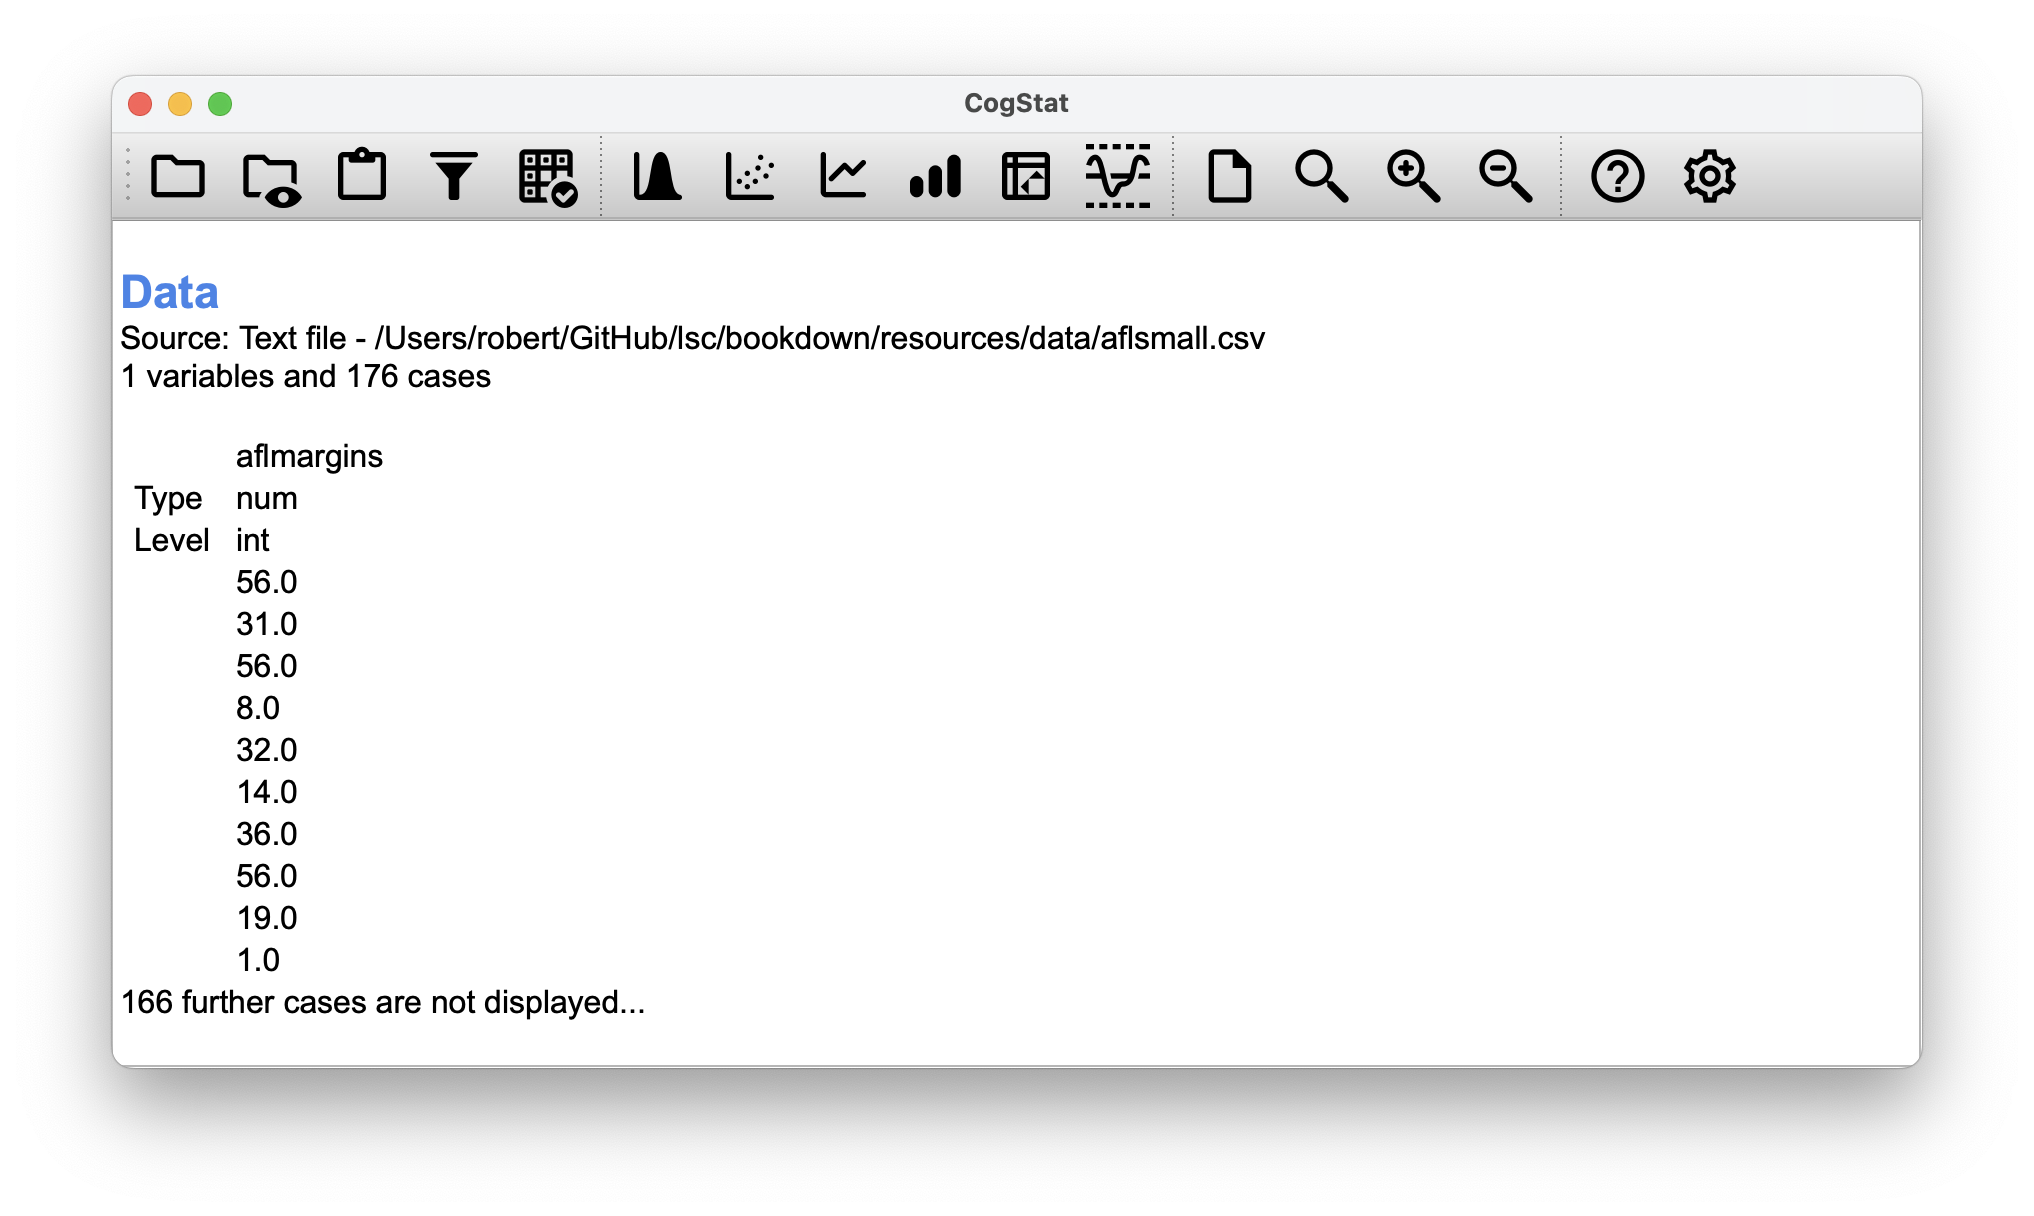
\includegraphics[width=0.66\linewidth]{resources/image/loadaflsmall} 

}

\caption[Loading `aflsmall.csv`]{Loading `aflsmall.csv`. This is what you would see after loading the dataset.}\label{fig:loadaflsmall}
\end{figure}

CogStat will help you get familiar with some essential aspects of your variable, like:

\begin{itemize}
\tightlist
\item
  measures of central tendency (mean, median)
\item
  measures of variability (range, minimum, maximum, standard deviation, quartiles)
\item
  measures of ``distortion'' (skewness, kurtosis).
\end{itemize}

These measures will help you contextualise the results so the conclusions drawn from the variable will be valid.

To start understanding a variable in CogStat, select \texttt{Explore\ variable} so a pop-up appears. Move the name of the data you wish to analyse (in this case: \texttt{aflmargins}) from \texttt{Available\ variables} to \texttt{Selected\ variables}, then click \texttt{OK} (Figure \ref{fig:explorevariabledialog}).

\begin{figure}

{\centering 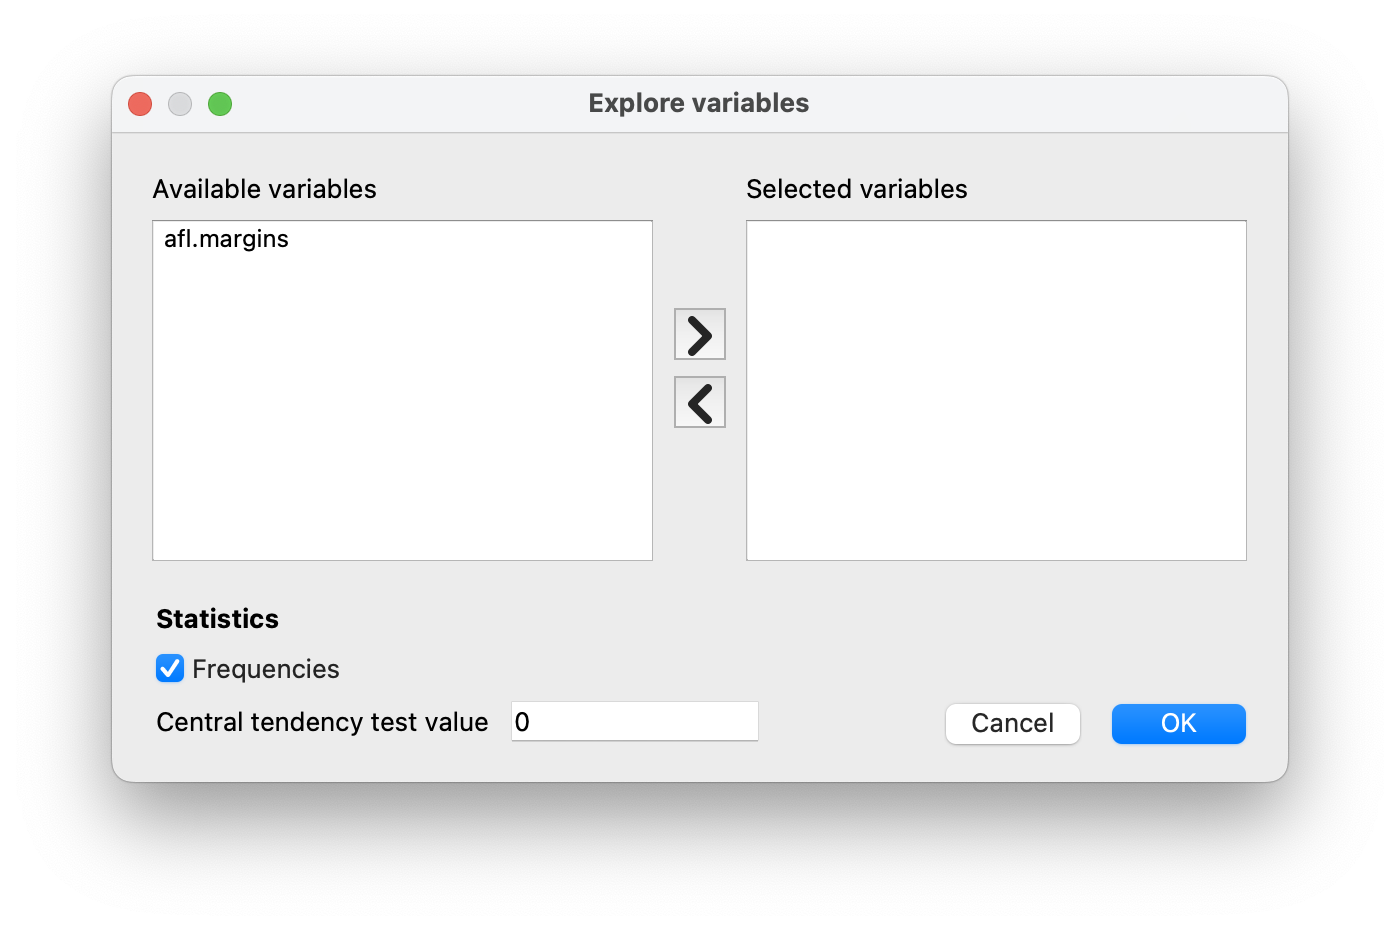
\includegraphics[width=0.66\linewidth]{resources/image/explorevariable} 

}

\caption{`Explore variable` dialogue.}\label{fig:explorevariabledialog}
\end{figure}

\begin{figure}

{\centering 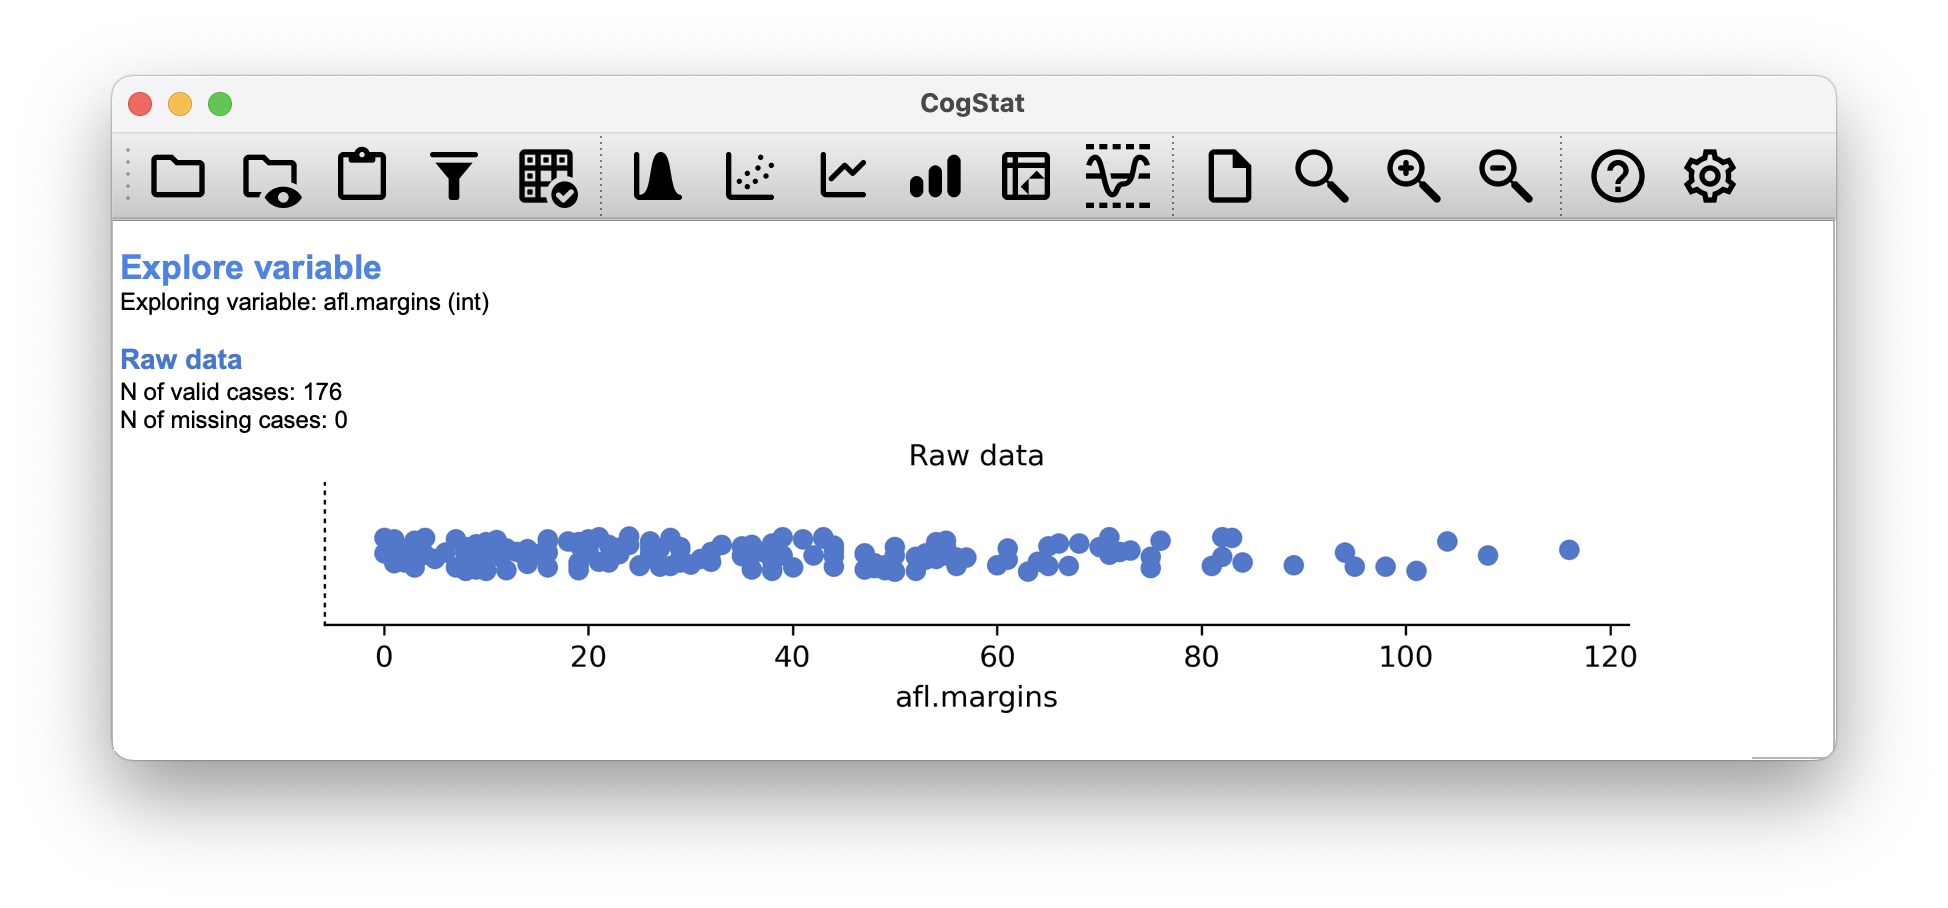
\includegraphics[width=0.66\linewidth]{resources/image/cogstatrawaflsmall} 

}

\caption[`Explore variable results` for the `aflsmall.csv` data set.]{`Explore variable results` for the `aflsmall.csv` data set. This is the first chart you will see exploring the raw shape of the data.}\label{fig:rawaflsmall}
\end{figure}

The first piece of information here is \(N\), which we will use to refer to the number of observations we're analysing. CogStat (or any other software for that matter) will only use valid data for calculations. Sometimes, when working with survey data, you will have missing data points, the number of which you might have to mention in your report. CogStat will quote these for you:

\begin{quote}
\texttt{N\ of\ valid\ cases:\ 176}\strut \\
\texttt{N\ of\ missing\ cases:\ 0}
\end{quote}

In the rest of this chapter, we will explore what these measures mean and what they indicate.

\hypertarget{centraltendency}{%
\section{Measures of central tendency}\label{centraltendency}}

In most situations, the first thing that you'll want to calculate is a measure of \textbf{\emph{central tendency}}. That is, you'd like to know something about the ``average'' or ``middle'' of your data lies.

\begin{center}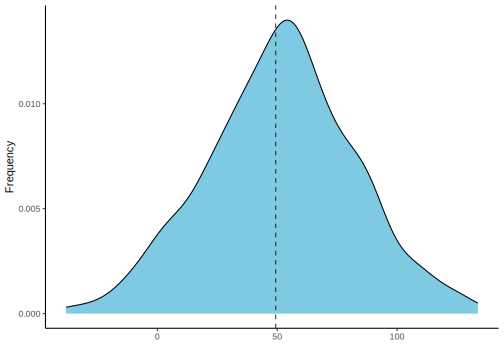
\includegraphics[width=0.66\linewidth]{lsc_files/figure-latex/unnamed-chunk-13-1} \end{center}

\hypertarget{mean}{%
\subsection{The mean}\label{mean}}

The first measure of \emph{central tendency} is the mean, or arithmetic average. It is calculated by adding up all of the values in the data set and then divide the sum by the total number (count) of values.

\begin{definition}[Mean]
\protect\hypertarget{def:defmean}{}\label{def:defmean}The \textbf{mean} of a set of observations is the sum of the observations divided by the number of observations.
\[
\bar{X} = \frac{\sum_{i=1}^N X_i}{N}
\]
\end{definition}

\begin{example}[Mean]
\protect\hypertarget{exm:exmean}{}\label{exm:exmean}The first five AFL margins were 56, 31, 56, 8 and 32 (which CogStat will display when loading the data, see Figure \ref{fig:loadaflsmall}), so the mean of these observations is just:
\[
\frac{56 + 31 + 56 + 8 + 32}{5} = \frac{183}{5} = 36.60
\]
\end{example}

Of course, this definition of the mean isn't news to anyone: averages (i.e., means) are used so often in everyday life that this is quite familiar.

We used \(N\) to denote the number of observations. Now let's attach a label to the observations themselves. It's traditional to use \(X\) for this, and to use subscripts to indicate which observation we're actually talking about. That is, we'll use \(X_1\) to refer to the first observation, \(X_2\) to refer to the second observation, and so on, all the way up to \(X_N\) for the last one. The following table lists the 5 observations in the \texttt{afl.margins} variable, along with the mathematical symbol used to refer to it, and the actual value that the observation corresponds to:

\begin{longtable}[]{@{}lcc@{}}
\toprule()
Observation & Symbol & Observed value \\
\midrule()
\endhead
winning margin, game 1 & \(X_1\) & 56 points \\
winning margin, game 2 & \(X_2\) & 31 points \\
winning margin, game 3 & \(X_3\) & 56 points \\
winning margin, game 4 & \(X_4\) & 8 points \\
winning margin, game 5 & \(X_5\) & 32 points \\
\bottomrule()
\end{longtable}

Okay, now let's try to write a formula for the mean. The goal here is to try to make sure that everyone reading this book is clear on the notation that we'll be using throughout the book. By tradition, we use \(\bar{X}\) as the notation for the mean, \(\scriptstyle\sum\) for the idea of summation, \(X_i\) for the \(i\)th observation, and \(N\) for the total number of observations. We're going to be re-using these symbols a fair bit, so you must understand them well enough to be able to ``read'' the equations and to be able to see what they're really saying.

So the calculation for the mean could be expressed using the following formula:
\[
\bar{X} = \frac{X_1 + X_2 + ... + X_{N-1} + X_N}{N}
\]

This formula is entirely correct, but it's terribly long, so we make use of the summation symbol \(\scriptstyle\sum\) to shorten it:
\[
\sum_{i=1}^5 X_i
\]

Taken literally, this could be read as ``the sum, taken over all \(i\) values from 1 to 5, of the value \(X_i\)''. But basically, what it means is ``add up the first five observations''. In any case, we can use this notation to write out the formula for the mean, which looks like this:
\[
\bar{X} = \frac{1}{N} \sum_{i=1}^N X_i 
\]

In all honesty, all this mathematical notation is just a fancy way of laying out the same things said in words: \emph{add all the values up, and then divide by the total number of items}.

\hypertarget{summation}{}
\begin{callout}

\begin{callouttitle}
\textbf{Summation symbol}: \(\scriptstyle\sum\) and \textbf{Product symbol}: \(\scriptstyle\prod\) notations

\end{callouttitle}

\nopagebreak

The summation symbol \(\scriptstyle\sum\) is used to denote the operation of adding up a sequence of numbers. It is used to write out formulas in a concise way, and is used extensively in mathematics.

\[
\sum_{i=1}^n X_i = X_1 + X_2 + ... + X_{n-1} + X_n
\]
where \(i\) is the \emph{index of the observation}, which means that the index starts out at the given number, so in this case, at the first observation (\(X_\mathbf{1}\)). The index is incremented by 1 for each observation (even if \(i>1\)), so the next observation is \(X_\mathbf{2}\), and so on, until the last observation, which is \(X_\mathbf{n}\), as denoted above the symbol.

The choice to use \(\Sigma\) to denote summation isn't arbitrary: it's the Greek upper case letter sigma, which is the analogue of the letter S in that alphabet.

Similarly, there's an equivalent symbol used to denote the multiplication of lots of numbers: because multiplications are also called ``products'', we use the \(\Pi\) symbol for this; the Greek upper case pi, which is the analogue of the letter P.

Check out more examples of \href{https://en.wikipedia.org/wiki/Summation\#Capital-sigma_notation}{summation notation} and \href{https://en.wikipedia.org/wiki/Multiplication\#Product_of_a_sequence}{product notation} on Wikipedia.

\end{callout}

CogStat calculates the mean automatically when exploring a variable using all valid data points, not just the first five. It will be part of the \texttt{Descriptives\ for\ the\ variable} section, as seen in Figure \ref{fig:histogramaflsmall}. The result for our variable is:

\begin{quote}
\texttt{afl.margins}\strut \\
\texttt{Mean\ 35.3}
\end{quote}

\begin{figure}

{\centering 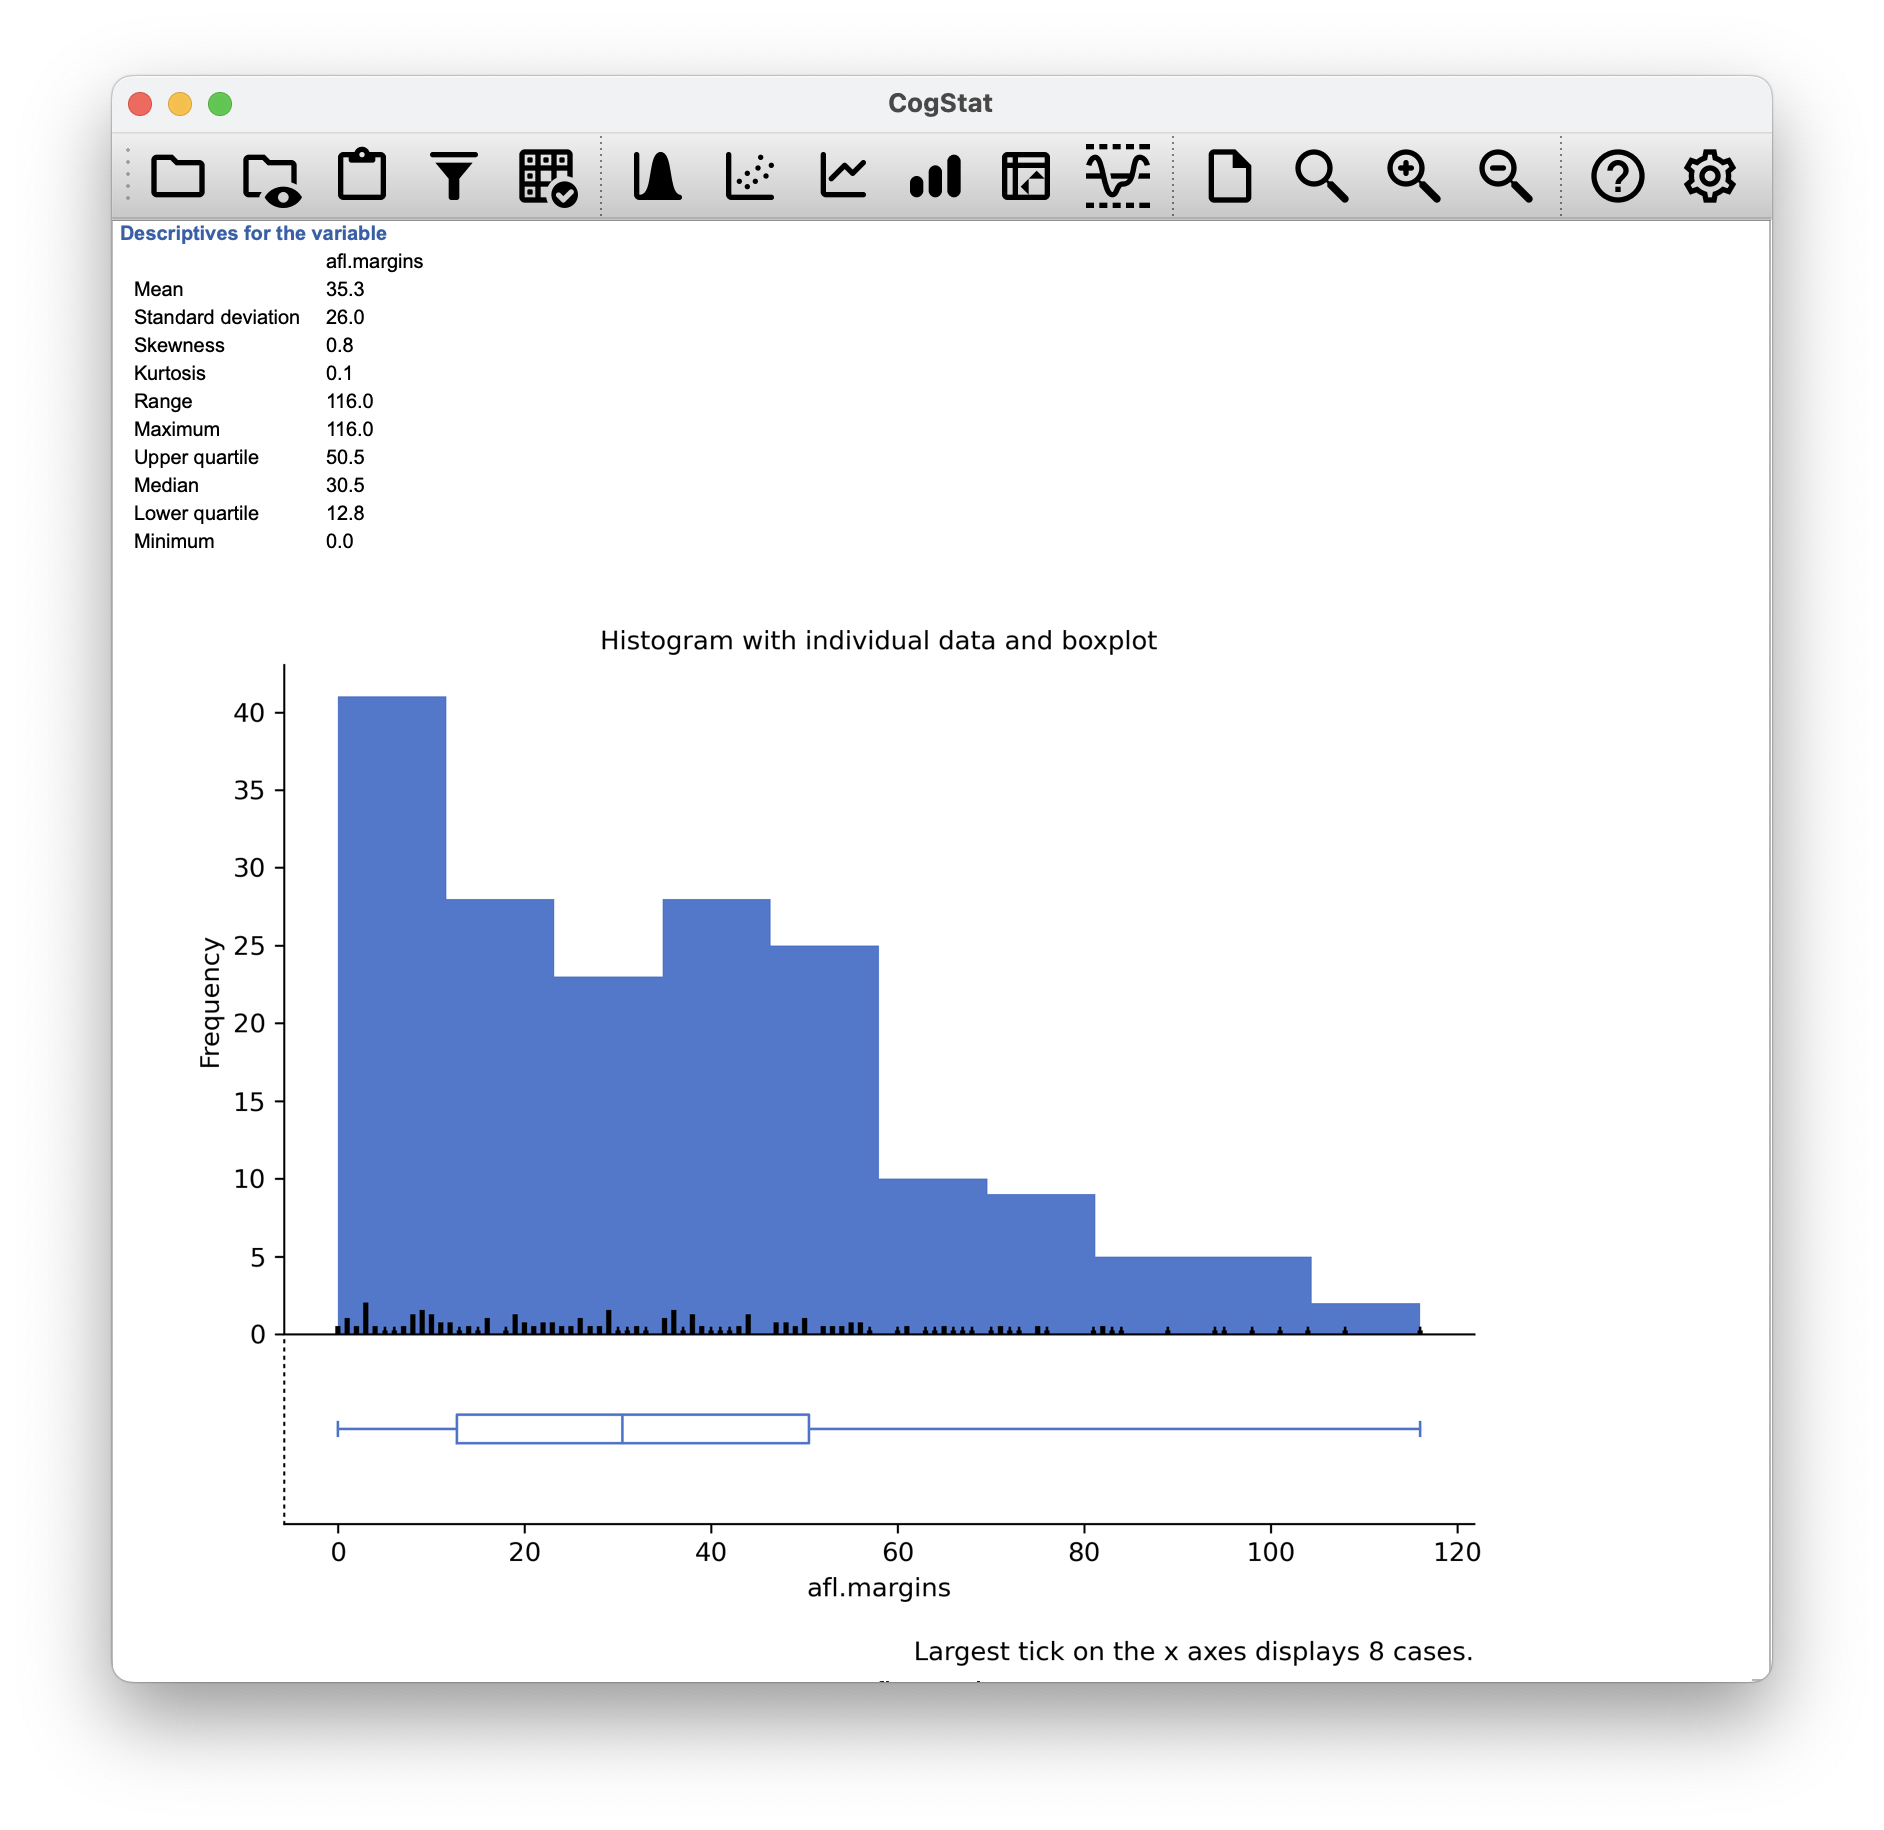
\includegraphics[width=0.66\linewidth]{resources/image/cogstathistogramaflsmall} 

}

\caption[Descriptive statistics and histogram for the `aflsmall.csv` data set.]{Descriptive statistics and histogram for the `aflsmall.csv` data set. Scrolling down, you'll see CogStat reporting all the descriptive measures while showing you a histogram to understand the shape of your data better. Drawing pictures of the data is an excellent way to convey the gist of what the data is trying to tell you; it's often instrumental to try to condense the data into a few simple summary statistics.}\label{fig:histogramaflsmall}
\end{figure}

\hypertarget{median}{%
\subsection{The median}\label{median}}

The second measure of \emph{central tendency} people use a lot is the median\footnote{\emph{medianus} is Latin for ``the one in the middle'', originating from the word \emph{medius}, meaning ``the middle''.}, and it's even easier to describe than the mean.

\begin{definition}[Median]
\protect\hypertarget{def:defmedian}{}\label{def:defmedian}The \textbf{median} is the middle value in a set of observations that has been arranged in ascending or descending order.
\end{definition}

\begin{example}[Median]
\protect\hypertarget{exm:exmedian}{}\label{exm:exmedian}As before, let's imagine we were interested only in the first 5 AFL winning margins: 56, 31, 56, 8 and 32. To figure out the median, we sort these numbers into ascending order. From inspection, it's evident that the median value of these five observations is 32 since that's the middle one in the sorted list.

\[
8, 31, \mathbf{32}, 56, 56
\]

But what should we do if we were interested in the first six games rather than the first 5? Since the sixth game in the season had a winning margin of 14 points, our sorted list is now:

\[
8, 14, \mathbf{31}, \mathbf{32}, 56, 56
\]

and there are \emph{two} middle numbers, \(31\) and \(32\). The median is defined as the average of those two numbers, which is \(31.5\).
\end{example}

In the data set we loaded to CogStat, there were 176 valid cases, so we ought to have two middle numbers. The result in this case is (as seen in Figure \ref{fig:histogramaflsmall}):

\begin{quote}
\texttt{afl.margins}\strut \\
\texttt{Median\ 30.5}
\end{quote}

\hypertarget{mean-or-median-whats-the-difference}{%
\subsection{Mean or median? What's the difference?}\label{mean-or-median-whats-the-difference}}

\begin{figure}

{\centering 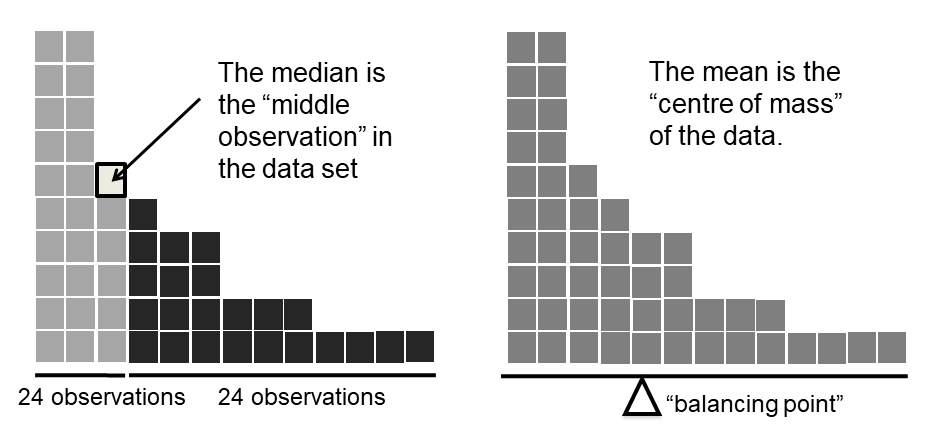
\includegraphics[width=0.66\linewidth]{./resources/image/meanmedian} 

}

\caption[An illustration of the difference between how the mean and the median should be interpreted.]{An illustration of the difference between how the mean and the median should be interpreted. The mean is basically the "centre of gravity" of the data set: if you imagine that the histogram of the data is a solid object, then the point on which you could balance it (as if on a see-saw) is the mean. In contrast, the median is the middle observation. Half of the observations are smaller, and half of the observations are larger.}\label{fig:meanmedian}
\end{figure}

Knowing how to calculate means and medians is only a part of the story. You also need to understand what each one is saying about the data, what that implies, and which one to choose. This is illustrated in Figure \ref{fig:meanmedian}; the mean is kind of like the ``centre of gravity'' of the data set, whereas the median is where you'd cut it in half. What this implies about which one you should use depends a little on what type of data you've got and what you're trying to achieve. As a rough guide:

\begin{itemize}
\tightlist
\item
  If your data are \emph{\protect\hyperlink{nominalscale}{nominal scale}}, you shouldn't be using either the mean or the median. Both the mean and the median rely on the idea that the numbers assigned to values are meaningful (i.e., 1 means 1 of a unit of measure, and not simply a technical coding for ``1: men, 2: women, 3: nonbinary \ldots{}''). If the numbering scheme is arbitrary, then use the mode (Section \ref{mode}) instead.
\item
  If your data are \emph{\protect\hyperlink{ordinalscale}{ordinal scale}}, you can to use the median but not the mean. The median only uses the order information in your data (i.e., which numbers are larger) which is the purpose of an ordinal scale. The mean makes use of the precise numeric values assigned to the observations beyond their order info, so it's not appropriate for ordinal data.
\item
  For \emph{\protect\hyperlink{intervalscale}{interval}} and \emph{\protect\hyperlink{ratioscale}{ratio scale}} data, either one is generally acceptable. Which one you pick depends a bit on what you're trying to achieve. The mean has the advantage of using all the information in the data (which is useful when you don't have a lot of data), but it's very susceptible to extreme values, as we'll see in Chapter \ref{trimmedmean}.
\end{itemize}

Let's expand on that last part a little. One consequence is that there are systematic differences between the mean and the median when the histogram is asymmetric (skewed; see Chapter \ref{skewnesskurtosis}). This is illustrated in Figure \ref{fig:meanmedian} notice that the median (right hand side) is located closer to the ``body'' of the histogram, whereas the mean (left hand side) gets dragged towards the ``tail'' (where the extreme values are).

\begin{example}[Mean or median]
\protect\hypertarget{exm:exmeanmedian}{}\label{exm:exmeanmedian}Suppose Bob (income \$50,000), Kate (income \$60,000) and Jane (income \$65,000) are sitting at a table: the average income at the table is \$58,333 and the median income is \$60,000. Then Bill sits down with them (income \$100,000,000). The average income has now jumped to \$25,043,750 but the median rises only to \$62,500. If you're interested in looking at the overall income at the table, the mean might be the right answer; but if you're interested in what counts as a typical income at the table, the median would be a better choice here.
\end{example}

\hypertarget{trimmedmean}{%
\subsection{Trimmed mean}\label{trimmedmean}}

\begin{example}[Outliers]
\protect\hypertarget{exm:exoutliers}{}\label{exm:exoutliers}Consider this rather strange-looking data set:
\[
-100,2,3,4,5,6,7,8,9,10
\]
If you were to observe this in a real-life data set, you'd probably suspect that there is something odd about the \(-100\) value. It's probably an \textbf{outlier}, a value that doesn't belong with the others. You might consider removing it from the data set entirely. In this particular case, it might be the right call. However, you don't always get such cut-and-dried examples. For instance, you might get this instead:
\[
-15,2,3,4,5,6,7,8,9,12
\]
The \(-15\) looks suspicious, but not as much as that \(-100\) did. In this case, it's a little trickier. It \emph{might} be a legitimate observation; it might not.
\end{example}

When faced with a situation where some of the most extreme-valued observations might not be quite trustworthy, the mean is not necessarily a good measure of central tendency. It is highly sensitive to one or two extreme values and might not be a \emph{robust} measure in all cases. One remedy is to use the median. An alternative solution is to use a \textbf{trimmed mean}.

\begin{definition}[Trimmed mean]
\protect\hypertarget{def:deftrimmedmean}{}\label{def:deftrimmedmean}A \textbf{trimmed mean} is a measure of central tendency, a type of average, that is calculated by discarding a certain percentage of the largest and smallest observations from the data, and then calculating the arithmetic average of the remaining observations.
\end{definition}

The goal is to preserve the best characteristics of the mean and the median: just like a median, you aren't highly influenced by extreme outliers. Generally, we describe a trimmed mean in terms of the percentage of observations on either side that are discarded. So, for instance, a 10\% trimmed mean discards the largest 10\% of the observations \emph{and} the smallest 10\% of the observations and then takes the mean of the remaining 80\% of the observations. Not surprisingly, the 0\% trimmed mean is just the regular mean, and the 50\% trimmed mean is the median. In that sense, trimmed means provide a whole family of central tendency measures that span the range from the mean to the median.

\begin{example}
\protect\hypertarget{exm:extrimmedmean}{}\label{exm:extrimmedmean}For our toy example above, we have 10 observations. So a 10\% trimmed mean is calculated by ignoring the largest value (i.e.~\(12\)) and the smallest value (i.e.~\(-15\)) and taking the mean of the remaining values.

\begin{quote}
\texttt{Mean:\ 4.1}\strut \\
\texttt{Median:\ 5.5}
\end{quote}

That's a fairly substantial difference. But the mean is being influenced too much by the extreme values at either end of the data set, especially the \(-15\) one. If we take a 10\% trimmed mean, we'll drop the extreme values on either side and take the mean of the rest:

\begin{quote}
\texttt{Mean:\ 5.5}
\end{quote}

Which, in this case, gives exactly the same answer as the median.
\end{example}

Currently, there is no direct way for you to do that in CogStat, but you can certainly trim those outlying data points in your source file and re-load the data.

\hypertarget{mode}{%
\subsection{Mode}\label{mode}}

\begin{definition}[Mode]
\protect\hypertarget{def:defmode}{}\label{def:defmode}The \textbf{mode} is a measure of central tendency that indicates the value that occurs most frequently in the data set.
\end{definition}

\begin{example}[Mode]
\protect\hypertarget{exm:exmode}{}\label{exm:exmode}

Consider the following data set:

\begin{quote}
0, 1, 1, 2, 3, 5, 8, 13, 21
\end{quote}

The mode would be 1, as it's the value the occurs most frequently. A \textbf{frequency table} helps you identify the mode in more complex datasets even if it's not calculated automatically.

\begin{quote}
Value: Frequency (Relative frequency)\\
0: 1 (11.1\%)\\
1: 2 (22.2\%)\\
2: 1 (11.1\%)\\
3: 1 (11.1\%)\\
5: 1 (11.1\%)\\
8: 1 (11.1\%)\\
13: 1 (11.1\%)\\
21: 1 (11.1\%)\\
\end{quote}

\end{example}

In CogStat, you will see a frequency table (Figure \ref{fig:freqaflsmall}) of the values in your data if you have \texttt{Frequencies} ticked in the \texttt{Explore\ variable} dialogue.

\begin{figure}

{\centering 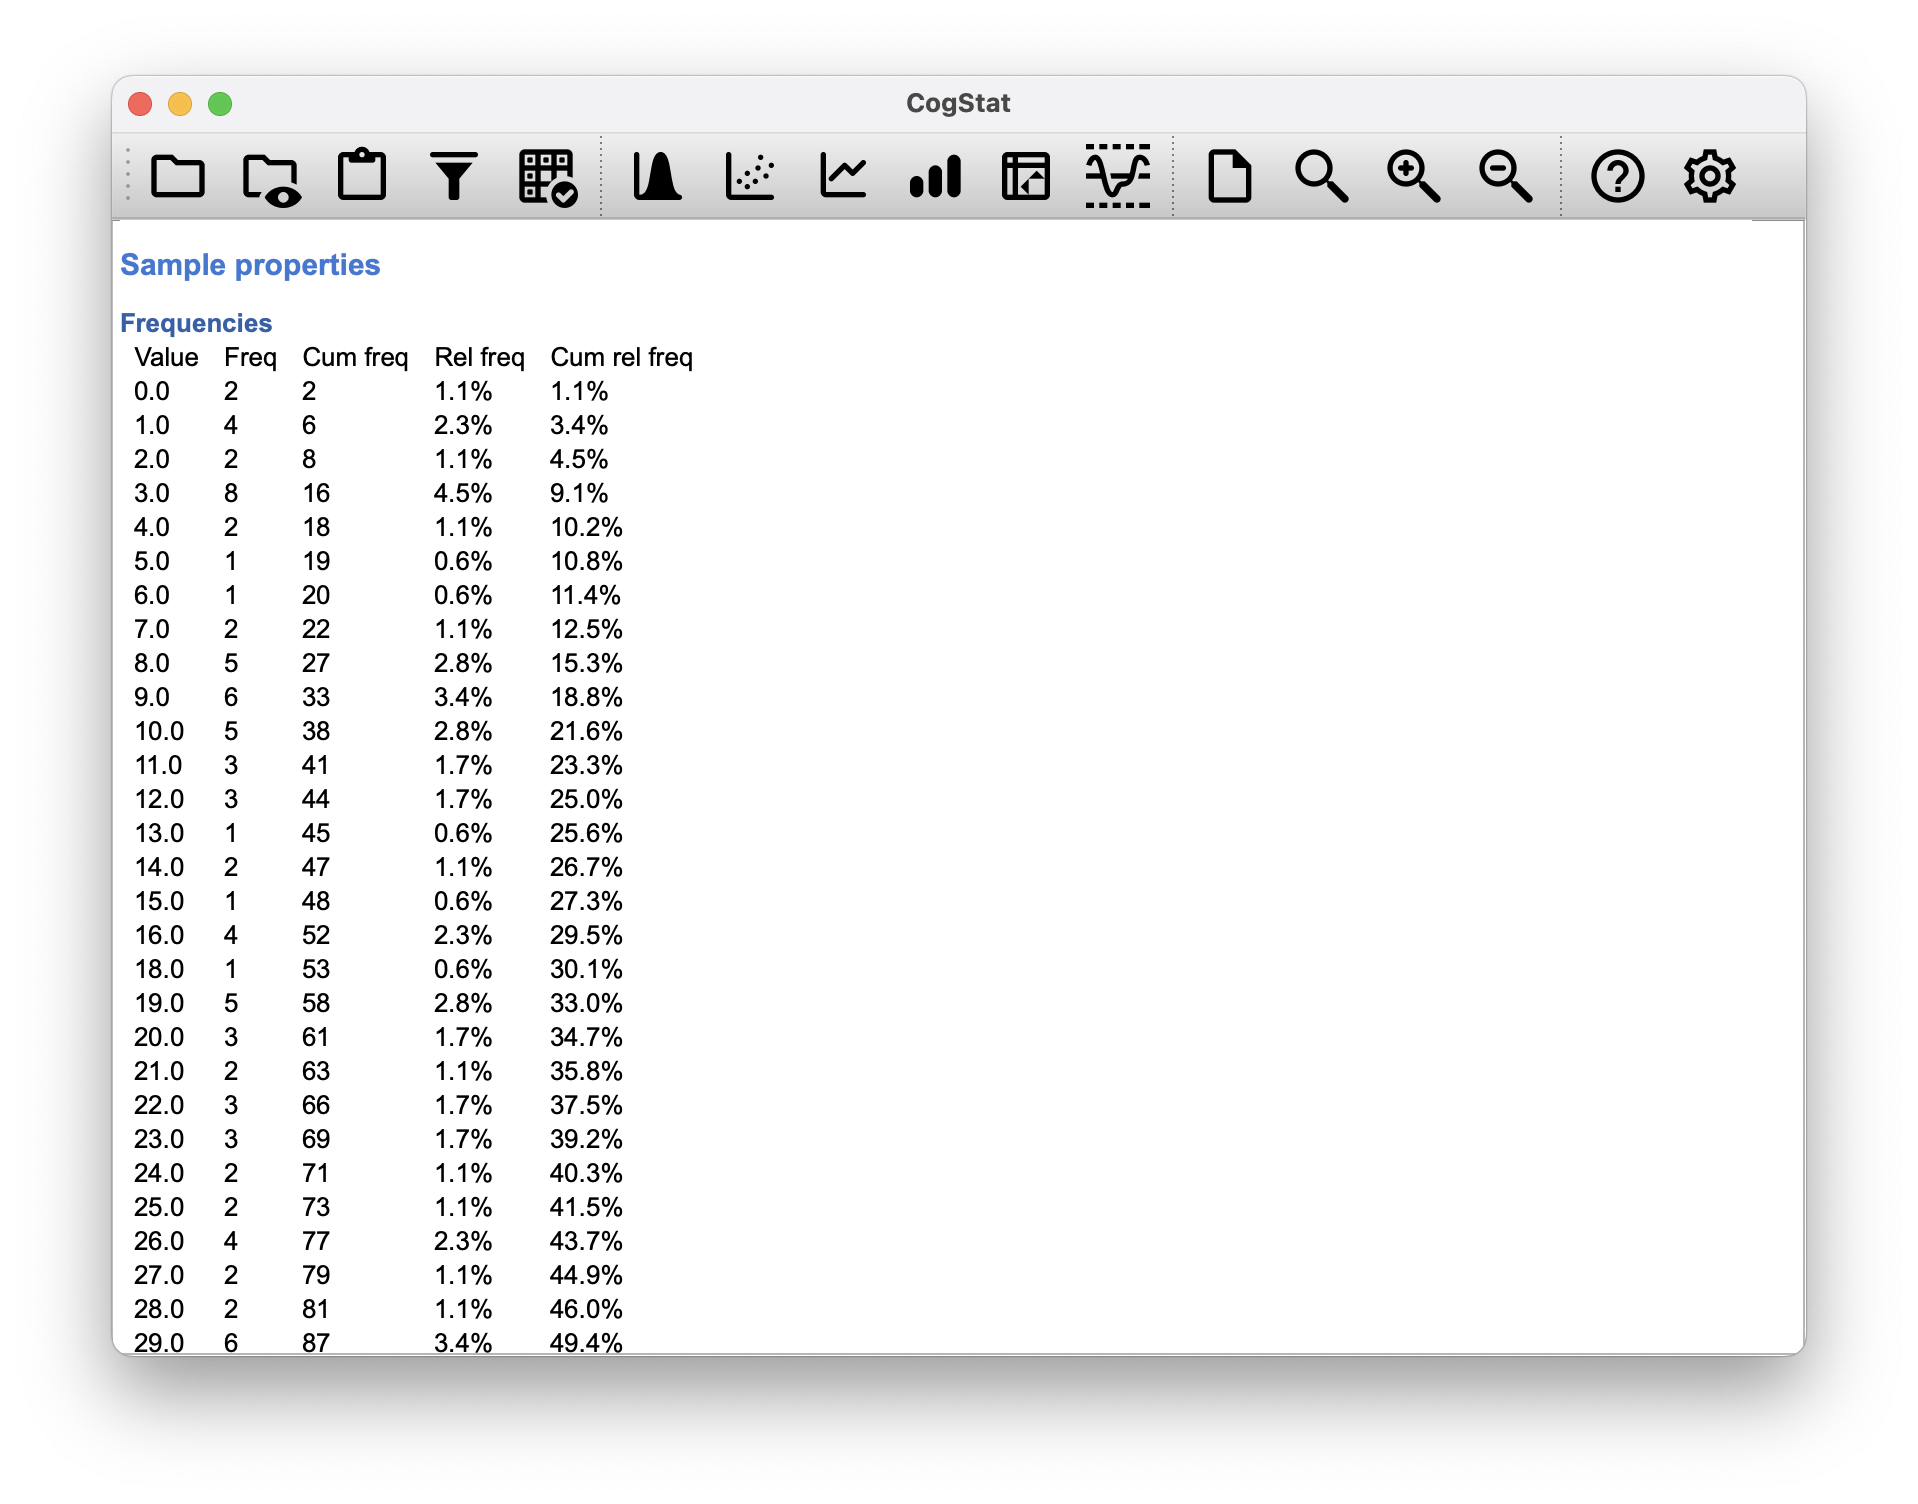
\includegraphics[width=0.66\linewidth]{resources/image/cogstatfrequencyaflsmall} 

}

\caption{The frequency table sorts non-nominal values from lowest to highest.}\label{fig:freqaflsmall}
\end{figure}

While it's generally true that the mode is most often calculated when you have \protect\hyperlink{nominalscale}{nominal scale} data -- because means and medians are useless for those sorts of variables --, there are some situations in which you do want to know the mode of an \protect\hyperlink{ordinalscale}{ordinal}, \protect\hyperlink{intervalscale}{interval} or \protect\hyperlink{ratioscale}{ratio scale} variable.

\begin{example}[Mode for ordinal, interval and ratio scale]
\protect\hypertarget{exm:exmode2}{}\label{exm:exmode2}Let's look at our \texttt{afl.margins} variable we loaded into CogStat. This variable is clearly ratio scale, and so in most situations the mean or the median is the measure of central tendency that you want. But consider that a friend of yours is offering a bet. They pick a football game at random, and without knowing who is playing you have to guess the \emph{exact} margin. If you guess correctly, you win \$50. If you don't, you lose \$1. There are no consolation prizes for ``almost'' getting the right answer. You have to guess exactly the right margin\footnote{This is called a ``0-1 loss function'', meaning that you either win (1) or you lose (0), with no middle ground.} For this bet, the mean and the median are completely useless to you. It is the mode that you should bet on. So, we look at the frequency table offered by the result set: the data suggest you should bet on a \(3.0\) point margin, and since this was observed in 8 of the 176 games (4.5\% of games -- the \emph{relative frequency}), the odds are firmly in your favour.
\end{example}

\hypertarget{var}{%
\section{Measures of variability}\label{var}}

The statistics that we've discussed so far all relate to \emph{central tendency}. They all talk about which values are ``in the middle'' or ``popular'' in the data. However, central tendency is not the only type of summary statistic that we want to calculate. The second thing that we really want is a measure of the \textbf{variability} (or, \emph{dispersion}) of the data. That is, how ``spread out'' are the data? How ``far'' away from the mean or median do the observed values tend to be?

\begin{figure}

{\centering 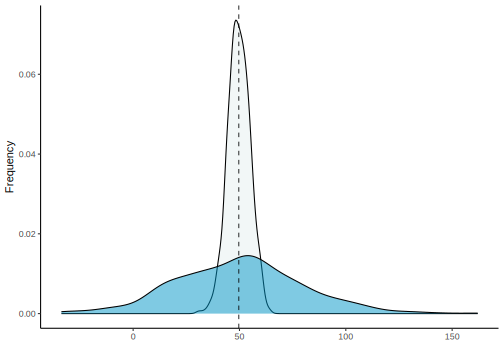
\includegraphics[width=0.66\linewidth]{lsc_files/figure-latex/unnamed-chunk-15-1} 

}

\caption{Data sets with the same mean but different dispersion.}\label{fig:unnamed-chunk-15}
\end{figure}

For now, let's assume that the data are interval or ratio scale, so we'll continue to use the \texttt{afl.margins} data. We'll use this data to discuss several different measures of spread, each with different strengths and weaknesses.

\hypertarget{range}{%
\subsection{Range}\label{range}}

\begin{definition}[Range]
\protect\hypertarget{def:defrange}{}\label{def:defrange}As a measure of variability, the \textbf{range} of a variable is the difference between the largest and smallest observation in the data set.
\[
\text{Range}=\max(x)-\min(x)
\]
\end{definition}

\begin{example}[Range]
\protect\hypertarget{exm:exrange}{}\label{exm:exrange}For the AFL winning margins data, the maximum value is \(116\), and the minimum is \(0\), so the range is:
\[116-0=\mathbf{116}\]
\end{example}

CogStat automatically calculates all these values (see Figure \ref{fig:histogramaflsmall}), so there is nothing we need to do about this, only to understand what it implies.

Although the range is the simplest way to quantify the notion of variability, it's not a fit-for-all tool. Recall from our discussion of the mean that we want our summary measure to be robust. If the data set has one or two extremely ``bad'' values in it (i.e., \emph{outliers}), we'd like our statistics not to be unduly influenced by these cases.

\begin{example}[Range with outliers present]
\protect\hypertarget{exm:exrange2}{}\label{exm:exrange2}Let us look once again at our toy example of a data set containing very extreme outliers:
\[
-100,2,3,4,5,6,7,8,9,10
\]

It is clear that the range is not robust since this has a range of \(110\), but if the outlier was removed, we would have a range of only \(8\).
\end{example}

\hypertarget{IQR}{%
\subsection{Interquartile range}\label{IQR}}

The \textbf{interquartile range} (IQR) is similar to the range in terms of measuring variability, but instead of calculating the difference between the largest and smallest value, it calculates the difference between the 25th and 75th quantile, hence, somewhat minimising the effect of a few outliers.

\begin{definition}[Interquartile range]
\protect\hypertarget{def:defIQR}{}\label{def:defIQR}The \textbf{interquartile range} (IQR) is the difference between the 25th and 75th quantile of a data set. It is a measure of variability that is less sensitive to outliers than the range.
\end{definition}

\hypertarget{calloutquantile}{}
\begin{callout}

\begin{callouttitle}
\textbf{Quantiles}

\end{callouttitle}

\nopagebreak

Quantiles are cut points that divide an ordered data set (or a distribution) into equal-sized groups of observations when the data is continuous. Or more generally, they cut a \protect\hyperlink{probability}{probability distribution} to equally probable intervals (see Chapter \ref{probability}).

For example, a data set of 40 observations can be divided into 4 equal-sized groups of 10 observations each.

\begin{longtable}[]{@{}cccc@{}}
\toprule()
Quantile & Number of observations & Lower bound & Upper bound \\
\midrule()
\endhead
1 & 10 & 1 & 10 \\
2 & 10 & 11 & 20 \\
3 & 10 & 21 & 30 \\
4 & 10 & 31 & 40 \\
\bottomrule()
\end{longtable}

This is called a \textbf{\emph{quartile}} (i.e., 1/4). If we wanted to define in percentages, this would be able to define 25th, 50th and 75th \textbf{\emph{percentiles}} of a data set. The \emph{25th percentile} (\emph{1st quartile} or \emph{lower quartile}) holds the value in a distribution that is greater than 25\% of the values and less than 75\% of the values. The \emph{50th percentile} (\emph{2nd quartile}) is the \emph{median}, and the \emph{75th percentile} (\emph{3rd quartile} or \emph{upper quartile}) is the value that is greater than 75\% of the values and less than 25\% of the values.

\begin{figure}

{\centering 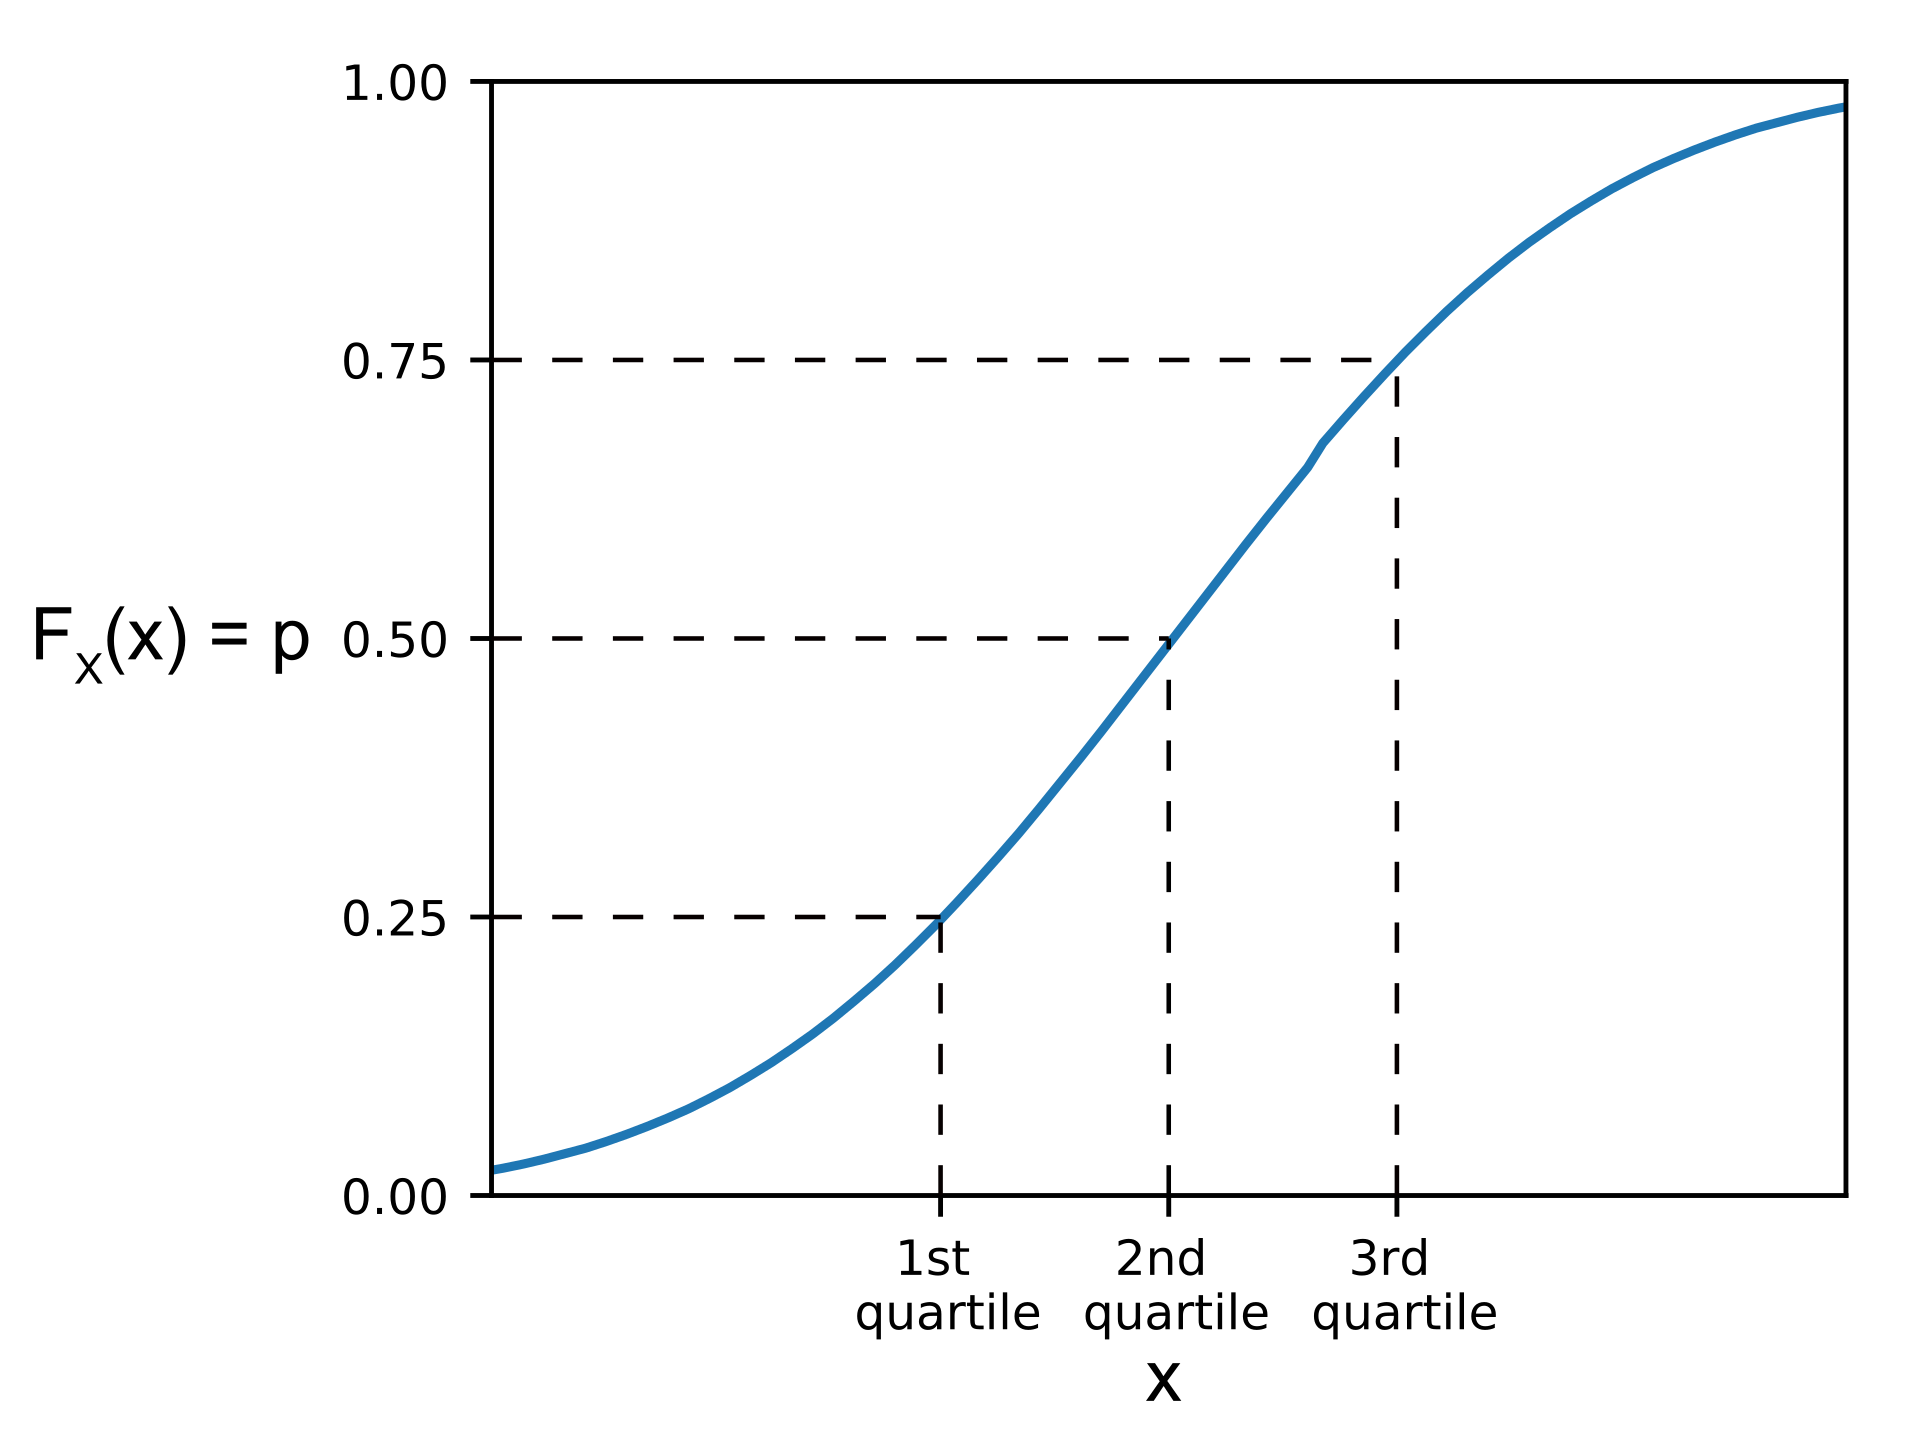
\includegraphics[width=0.45\linewidth]{resources/image/1920px-NormalCDFQuartile3} 

}

\caption{The 25th, 50th and 75th percentiles of a cumulative distribution of a normal distribution. (StevenJYang on [Wikipedia: Quartile](https://en.wikipedia.org/wiki/Quartile))}\label{fig:unnamed-chunk-17}
\end{figure}

The data can be divided into other quantiles as well: e.g.~a distribution cut in 5 equal-sized groups are called \textbf{\emph{quintiles}}, and a distribution cut in 10 equal-sized groups are called \textbf{\emph{deciles}}, and so on.

There are different methods to cutting discrete data into quantiles, but we're not going to discuss them here.

\end{callout}

CogStat provides you with both the 25th (\texttt{Lower\ quartile}) and 75th quantiles (\texttt{Upper\ quartile}) automatically:

\begin{quote}
\texttt{Upper\ quartile:\ 50.5}\strut \\
\texttt{Lower\ quartile:\ 12.8}
\end{quote}

\begin{example}[Interquartile range]
\protect\hypertarget{exm:exIQR}{}\label{exm:exIQR}We can see that the interquartile range for the 2010 AFL winning margins data is:
\[
50.5 - 12.8 = \mathbf{37.7}
\]
\end{example}

While it's obvious how to interpret the range, it's a little less obvious how to interpret the IQR. The simplest way to think about it is like this: the interquartile range is the range spanned by the ``middle half'' of the data, ignoring any data between \(-\infty\) and \(Q_1\), and between \(Q_3\) and \(+\infty\). That is, one quarter of the data falls below the 25th percentile, one quarter of the data is above the 75th percentile, leaving the ``middle half'' of the data lying in between the two. And the IQR is the range covered by this middle half.

\hypertarget{boxplot}{}
\begin{callout}

\begin{callouttitle}
\textbf{Boxplots}

\end{callouttitle}

\nopagebreak

Boxplots (or ``box and whiskers'' plots) are a standardised method to display the distribution of a data set based on a five-number summary:

\begin{itemize}
\tightlist
\item
  the minimum and maximum (i.e., range),
\item
  first quartile and third quartile (i.e., IQR),
\item
  and the median.
\end{itemize}

\begin{figure}

{\centering 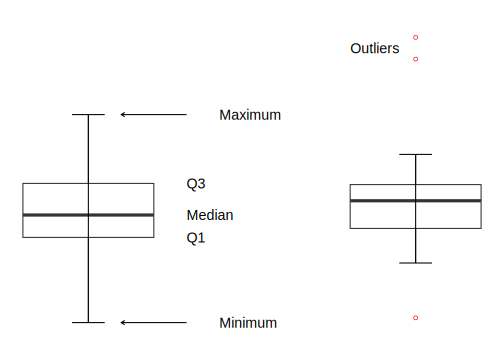
\includegraphics[width=0.75\linewidth]{lsc_files/figure-latex/unnamed-chunk-18-1} 

}

\caption{Boxplot explained}\label{fig:unnamed-chunk-18}
\end{figure}

Like histograms, they're most suited to interval or ratio scale data. Some boxplots separate out those observations that are ``suspiciously'' distant from the rest of the data, i.e., the outliers. These are usually displayed with a circle or a dot.

\end{callout}

\hypertarget{aad}{%
\subsection{Mean absolute deviation (average absolute deviation)}\label{aad}}

The two measures we've looked at so far, the range and the interquartile range, both rely on the idea that we can measure the spread of the data by looking at quantiles. However, this isn't the only way to think about the problem. A different approach is to select some meaningful reference point (usually the mean or the median) and then report the ``typical'' deviations from that. In practice, this leads to two different measures, the ``mean absolute deviation'' (from the mean) and the ``median absolute deviation'' (from the median). Irritatingly, ``mean absolute deviation'' and ``median absolute deviation'' have the same acronym (i.e., MAD), which leads to a certain amount of ambiguity. What we'll do is use \emph{AAD} (\emph{average absolute deviation}) for \emph{mean absolute deviation}, while \emph{MAD} will stand for \emph{median absolute deviation}.

\begin{definition}[Average absolute deviation]
\protect\hypertarget{def:defAAD}{}\label{def:defAAD}The \textbf{average absolute deviation} (AAD) is a measure of variability calculated as the average of the absolute difference between each observation and the \emph{mean} of the data set.
\[
\text{AAD} = \frac{1}{n} \sum_{i=1}^n |X_i - \bar{X}|
\]
where \(n\) is the number of observations, \(X_i\) is the \(i\)th observation, and \(\bar{X}\) is the mean of the data set.
\end{definition}

\begin{example}[Average absolute deviation]
\protect\hypertarget{exm:exAAD}{}\label{exm:exAAD}Let's think about our AFL winning margins data, and once again we'll start by pretending that there's only 5 games in total, with winning margins of 56, 31, 56, 8 and 32. Our calculations rely on an examination of the deviation from some reference point, in this case, the mean.

\begin{enumerate}
\def\labelenumi{\arabic{enumi}.}
\tightlist
\item
  The first thing we need to look up is the mean, \(\bar{X}\). For these five observations, our mean is \(\bar{X} = 36.6\).
\item
  The next step is to convert each of our observations \(X_i\) into a deviation score. We do this by calculating the difference between the observation \(X_i\) and the mean \(\bar{X}\) (i.e., the deviation score: \(X_i - \bar{X}\)).
\item
  Then we convert these deviations to absolute deviations. Mathematically, we would denote the absolute value of \(-3\) as \(|-3|\), and so we say that \(|-3| = 3\). We use the absolute value function here because we don't care whether the value is higher than the mean or lower than the mean; we're just interested in how \emph{close} it is to the mean.
\end{enumerate}

To help make this process as obvious as possible, the table below shows these calculations for all five observations:

\begin{longtable}[]{@{}lllll@{}}
\toprule()
Observation & Symbol & Observed value & Deviation score \(X_i - \bar{X}\) & Absolute d.s. \(|X_i - \bar{X}|\) \\
\midrule()
\endhead
winning margin, game 1 & \(X_1\) & 56 points & 56 - 36.6 = 19.4 & 19.4 \\
winning margin, game 2 & \(X_2\) & 31 points & 31 - 36.6 = -5.6 & 5.6 \\
winning margin, game 3 & \(X_3\) & 56 points & 56 - 36.6 = 19.4 & 19.4 \\
winning margin, game 4 & \(X_4\) & 8 points & 8 - 36.6 = -28.6 & 28.6 \\
winning margin, game 5 & \(X_5\) & 32 points & 32 - 36.6 = -4.6 & 4.6 \\
\bottomrule()
\end{longtable}

Now that we have calculated the absolute deviation score for every observation in the data set, we only have to calculate the mean of these scores. Let's do that:
\[
\frac{19.4 + 5.6 + 19.4 + 28.6 + 4.6}{5} = 15.52
\]
And we're done. The mean absolute deviation for these five scores is 15.52.
\end{example}

Currently, AAD is not calculated in CogStat, but you can calculate this with other statistics software. When this is added, we'll update this section.

\hypertarget{mad}{%
\subsection{Median absolute deviation}\label{mad}}

The basic idea behind \emph{median absolute deviation} (MAD) is identical to the one behind the mean absolute deviation (Section \ref{aad}). The difference is that you use the median. This has a straightforward interpretation: every observation in the data set lies some distance away from the typical value (the median). So the MAD is an attempt to describe a \emph{typical deviation from a typical value} in the data set.

\begin{definition}[Median absolute deviation]
\protect\hypertarget{def:defMAD}{}\label{def:defMAD}The \textbf{median absolute deviation} (MAD) is a measure of variability calculated as the average of the absolute difference between each observation and the \emph{median} of the data set.

\[
\text{MAD} = \frac{1}{n} \sum_{i=1}^n |X_i - \text{median}(X)|
\]

where \(n\) is the number of observations, \(X_i\) is the \(i\)th observation, and \(\text{median}(X)\) is the median of the data set.
\end{definition}

\begin{example}[Median absolute deviation]
\protect\hypertarget{exm:exMAD}{}\label{exm:exMAD}Let's think about our AFL winning margins data, and once again we'll start by pretending that there's only 5 games in total, with winning margins of 56, 31, 56, 8 and 32. Our calculations rely on an examination of the deviation from some reference point, in this case, the median. The median for these five observations is \(\text{median}(X) = 32\). We'll repeat the same steps as before with the \protect\hyperlink{exAAD}{mean absolute deviation}, and we'll have the following result:

\[
\text{MAD} = \frac{1}{5} \left( |56 - 32| + |31 - 32| + |56 - 32| + |8 - 32| + |32 - 32| \right) = 19.5
\]
\end{example}

\hypertarget{variance}{%
\subsection{Variance}\label{variance}}

Variance isn't all too different from the \protect\hyperlink{aad}{mean absolute deviation}. The main difference is that we use squared deviations instead of absolute deviations. With squared deviations, we obtain a measure called \textbf{variance}.

\begin{definition}[Variance]
\protect\hypertarget{def:defVar}{}\label{def:defVar}\textbf{Variance} is a measure of variability calculated as the average of the \emph{squared difference} between each observation and the \emph{mean} of the data set.

\[
\mbox{Var}(X) = \frac{1}{n} \sum_{i=1}^n (X_i - \bar{X})^2
\]

where \(n\) is the number of observations, \(X_i\) is the \(i\)th observation, and \(\bar{X}\) is the mean of the data set.
\end{definition}

\hypertarget{calloutVar}{}
\begin{callout}

\begin{callouttitle}
\textbf{Population variance versus variance estimate}

\end{callouttitle}

\nopagebreak

If you are extremely lucky and have a data set that contains the entire population, then you can calculate the variance as given in Definition \ref{def:defVar}. This is called \textbf{population variance}. In this case the variance is denoted \(\sigma^2\), the mean is denoted as \(\mu\).

\[
\sigma^2 = \frac{1}{n} \sum_{i=1}^n (X_i - \mu)^2
\]

In research, however, you are most likely to have gathered data for merely a \emph{sample} of the population. There is an alternative formula for this case. This is called \textbf{variance estimate}, or \emph{estimated variance}, or \emph{sample variance}, or \emph{estimated population variance}, and is denoted \(s^2\). The formula for the variance estimate is:

\[
s^2 = \frac{1}{n-1} \sum_{i=1}^n (X_i - \bar{X})^2
\]

where \(n\) is the number of observations in the sample, \(X_i\) is the \(i\)th observation, and \(\bar{X}\) is the mean of the sample. You'll notice the difference is the denominator using \(n-1\) instead of \(n\).

\end{callout}

Variances are \emph{additive}. Suppose we have two variables (\(X\) and \(Y\)), whose variances are \(\mbox{Var}(X)\) and \(\mbox{Var}(Y)\) respectively. Now imagine we want to define a new variable \(Z\) that is the sum of the two, \(Z = X+Y\). As it turns out, the variance of \(Z\) is equal to \(\mbox{Var}(X) + \mbox{Var}(Y)\).

\begin{example}[Additive property of the variance]
\protect\hypertarget{exm:exVarAddit}{}\label{exm:exVarAddit}Let's use the first five AFL games as our data. If we follow the same approach that we took last time, we end up with the following table:

\begin{table}[H]
\centering
\resizebox{\linewidth}{!}{
\begin{tabular}{llcc}
\toprule
\multicolumn{1}{c}{Which game} & \multicolumn{1}{c}{Value} & \multicolumn{1}{c}{Deviation from mean} & \multicolumn{1}{c}{Absolute squared deviation} \\
\cmidrule(l{3pt}r{3pt}){1-1} \cmidrule(l{3pt}r{3pt}){2-2} \cmidrule(l{3pt}r{3pt}){3-3} \cmidrule(l{3pt}r{3pt}){4-4}
$i$ & $X_i$ & $X_i - \bar{X}$ & $(X_i - \bar{X})^2$\\
\midrule
1 & 56 & 19.4 & 376.36\\
2 & 31 & -5.6 & 31.36\\
3 & 56 & 19.4 & 376.36\\
4 & 8 & -28.6 & 817.96\\
5 & 32 & -4.6 & 21.16\\
\bottomrule
\end{tabular}}
\end{table}

That last column contains all of our squared deviations, so all we have to do is average them.

\[
\frac{( 376.36 + 31.36 + 376.36 + 817.96 + 21.16 )}{5} = 324.64
\]
\end{example}

Let's tackle the burning question you're probably thinking: how do you \emph{interpret} the variance? Unfortunately, the reason why we haven't given you the human-friendly interpretation of the variance is that there really isn't one. It does have some elegant mathematical properties that suggest that it really is a fundamental quantity for expressing variation and spread. The reason for the difficulty is that all the numbers have been squared, and they don't necessarily mean anything in the original units. For example, if you're running an analysis on vitamin D levels in a study about mood disorders, you'll have a base unit of measure of nmol/L or ng/mL. If you square these numbers, you'll end up with a variance in nmol/L-squared or ng/mL-squared. This is a meaningless unit of measure on its own. However, variance is still a good measure to indicate a spread of data, and it's a good measure to use when comparing variances between different groups.

CogStat will not attempt to interpret the variance nor will it give you the raw value.

\hypertarget{sd}{%
\subsection{Standard deviation}\label{sd}}

Suppose you would like to have a measure expressed in the same units as the data itself (i.e.~nmol/L, not nmol/L-squared). What should you do? The solution to the problem is obvious: take the square root of the variance, known as the \textbf{standard deviation} (usually shortened as \emph{SD} or \emph{Std dev.}), also called the \emph{root mean squared deviation}, or RMSD. This solves our problem with variance fairly neatly: it's much easier to understand ``a standard deviation of 18.01 nmol/L'' since it's expressed in the original units.

\begin{definition}[Standard deviation]
\protect\hypertarget{def:defSD}{}\label{def:defSD}\textbf{Standard deviation} is the \emph{square root} of the average of the \emph{squared difference} between each observation and the \emph{mean} of the data set.

\[
\mbox{SD} = \sqrt{ \frac{1}{n} \sum_{i=1}^n \left( X_i - \bar{X} \right)^2 }
\]
\end{definition}

\hypertarget{calloutSD}{}
\begin{callout}

\begin{callouttitle}
\textbf{Population SD versus estimated SD}

\end{callouttitle}

\nopagebreak

Similarly to variance, we can differentiate the formula for a population-based standard deviation and a sample-based standard deviation.

The \textbf{population SD} is denoted \(\sigma\), the mean is denoted as \(\mu\).

\[
\sigma = \sqrt{ \frac{1}{n} \sum_{i=1}^n \left( X_i - \mu \right)^2 }
\]

For calculating a population \emph{estimate} based on sample data, we use the \textbf{estimated standard deviation} (\(s\)) formula.

\[
s = \sqrt{ \frac{1}{n-1} \sum_{i=1}^n \left( X_i - \bar{X} \right)^2 }
\]

where \(n\) is the number of observations in the sample, \(X_i\) is the \(i\)th observation, and \(\bar{X}\) is the mean of the sample. The denominator is \(n-1\) instead of \(n\).

\end{callout}

So how do we interpret standard deviation? Standard deviation has the same unit of measure as the observations, e.g., nmol/L, but just like variance, it doesn't have a simple interpretation either. The interpretation is based on the scale of the measurement. E.g. 3.5 can be big or small depending on the scale of measurement. For example, a 3.5 nmol/L SD value for vitamin D level suggests a fairly consistent measurement, considering 50-75 nmol/L is adequate, \textgreater75 is optimum, and \textless25 is deficient according to NHS UK guidelines\footnote{\url{https://www.southtees.nhs.uk/services/pathology/tests/vitamin-d/}} in 2023. But an SD of 3.5 for a 5-level Likert scale is massive, indicating a less consistent data point and high variability.

There are different ways to standardise the SD. One way is to divide the SD by the mean, which gives you the \textbf{coefficient of variation} (CV). Another way is by utilizing \(z\)-scores which assumes the data are \emph{normally} distributed, which is an important concept discussed in Chapter \ref{probability}. We'll discuss z-scores shortly in Chapter \ref{zscore}.

\hypertarget{which-measure-to-use}{%
\subsection{Which measure to use?}\label{which-measure-to-use}}

We've discussed quite a few measures of spread and hinted at their strengths and weaknesses. Here's a quick summary:

\begin{itemize}
\tightlist
\item
  \protect\hyperlink{range}{\emph{Range}}. Gives you the full spread of the data. It's very vulnerable to outliers, and as a consequence, it isn't often used unless you have good reasons to care about the extremes in the data.
\item
  \protect\hyperlink{IQR}{\emph{Interquartile range}}. Tells you where the ``middle half'' of the data sits. It's pretty robust and complements the median nicely. This is used a lot.
\item
  \protect\hyperlink{AAD}{\emph{Average absolute deviation}}. Tells you how far ``on average'' the observations are from the mean. It's very interpretable but has a few minor issues that make it less attractive to statisticians than the standard deviation. Used sometimes, but not often.
\item
  \protect\hyperlink{MAD}{\emph{Median absolute deviation}}. The typical deviation from the median value.
\item
  \protect\hyperlink{variance}{\emph{Variance}}. Tells you the average squared deviation from the mean. It's mathematically elegant and is probably the ``right'' way to describe variation around the mean, but it's completely uninterpretable because it doesn't use the same units as the data. Almost never used except as a mathematical tool, but it's buried ``under the hood'' of a very large number of statistical tools.
\item
  \protect\hyperlink{sd}{\emph{Standard deviation}}. This is the square root of the variance. It's fairly elegant mathematically, and it's expressed in the same units as the data, so it can be interpreted pretty well. In situations where the mean is the measure of central tendency, this is the default. This is by far the most popular measure of variation.
\end{itemize}

In short, the IQR and the standard deviation are easily the two most common measures used to report the variability of the data. Still, there are situations in which range or other measures are used.

\hypertarget{skewnesskurtosis}{%
\section{Skewness and kurtosis}\label{skewnesskurtosis}}

There are two more descriptive statistics that you will likely see reported in the psychological literature, known as \textbf{skewness} and \textbf{kurtosis}. These are measures of the shape of the distribution of the data.

\begin{figure}

{\centering 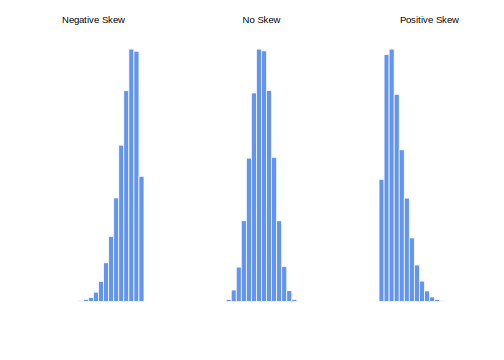
\includegraphics[width=0.66\linewidth]{lsc_files/figure-latex/skewness-1} 

}

\caption[An illustration of skewness.]{An illustration of skewness. On the left we have a negatively skewed data set (skewness $= -.93$), in the middle we have a data set with no skew (technically, skewness $= -.006$), and on the right we have a positively skewed data set (skewness $= .93$).}\label{fig:skewness}
\end{figure}

\begin{definition}[Skewness]
\protect\hypertarget{def:defskewness}{}\label{def:defskewness}\textbf{Skewness} is a measure of assymetry of a distribution that compares the median and mean to the mode. A negative skew means the median and mean are smaller than the mode, resulting in a long tail on the left. A positive skew means the median and mean are larger than the mode, resulting in a long tail on the right. A skewness of 0 means the median and mean are equal to the mode, resulting in a symmetrical distribution.

\[
\mbox{skewness}(X) = \frac{1}{N \hat{\sigma}^3} \sum_{i=1}^N (X_i - \bar{X})^3
\]

where \(N\) is the number of observations, \(\bar{X}\) is the sample mean, and \(\hat{\sigma}\) is the standard deviation (the ``divide by \(N-1\)'' version, that is).
\end{definition}

As Figure \ref{fig:skewness} illustrates, if the data tend to have a lot of extreme small values (i.e., the lower tail is ``longer'' than the upper tail) and not so many extremely large values (left panel), then we say that the data are \emph{negatively skewed}. On the other hand, if there are more extremely large values than extremely small ones (right panel) we say that the data are \emph{positively skewed}.

Not surprisingly, it turns out that the AFL winning margins data is fairly skewed: \(0.8\) (see Figure \ref{fig:histogramaflsmall} depicting the analysis results from CogStat).

\begin{definition}[Kurtosis]
\protect\hypertarget{def:defkurtosis}{}\label{def:defkurtosis}\textbf{Kurtosis} describes the degree of steepness of a distribution. A steep distribution is \emph{leptokurtic} (positive kurtosis) distribution, a flat distribution is \emph{platykurtic} (negative kurtosis), and the normal distribution is \emph{mesokurtic} (kurtosis is 0).

\[
\mbox{kurtosis}(X) = \frac{1}{N \hat\sigma^4} \sum_{i=1}^N \left( X_i - \bar{X} \right)^4 - 3
\]

where \(N\) is the number of observations, \(\bar{X}\) is the sample mean, and \(\hat{\sigma}\) is the standard deviation (the ``divide by \(N-1\)'' version, that is).
\end{definition}

\textbf{Kurtosis}, put simply, is a measure of the ``pointiness'' of a data set, as illustrated in Figure \ref{fig:kurtosis}.

\begin{figure}

{\centering 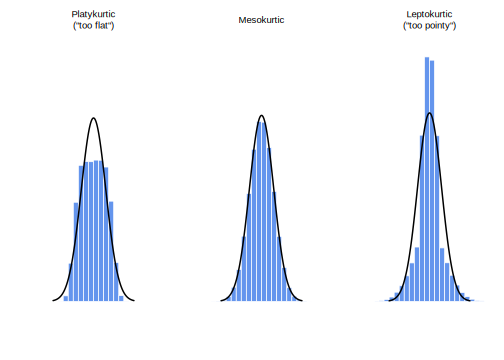
\includegraphics[width=0.66\linewidth]{lsc_files/figure-latex/kurtosis-1} 

}

\caption{An illustration of kurtosis. On the left, we have a "platykurtic" data set (kurtosis = $-.95$), meaning that the data set is "too flat". In the middle we have a "mesokurtic" data set (kurtosis is almost exactly 0), which means that the pointiness of the data is just about right. Finally, on the right, we have a "leptokurtic" data set (kurtosis $= 2.12$) indicating that the data set is "too pointy". Note that kurtosis is measured with respect to a normal curve (black line)}\label{fig:kurtosis}
\end{figure}

When reading the automatically calculated kurtosis value from our CogStat result set, we discover that the AFL winning margins data is just pointy enough: \(0.1\).

\hypertarget{zscore}{%
\section{\texorpdfstring{Standard scores (\(z\)-score)}{Standard scores (z-score)}}\label{zscore}}

Suppose a friend is creating a new questionnaire to measure ``grumpiness''. The survey has 50 questions, which you can answer in a grumpy way or not. Across a big sample (hypothetically, let's imagine a million people or so!), the data are fairly normally distributed, with the mean grumpiness score being 17 out of 50 questions answered in a grumpy way and the standard deviation is 5. In contrast, when we take the questionnaire, we answer 35 out of 50 questions in a grumpy way. So, how grumpy are we? One way to think about it would be to say that we have a grumpiness of 35/50, so you might say that we're 70\% grumpy. But that's a bit weird when you think about it. Suppose our friend had phrased her questions a bit differently. In that case, people might have answered them differently, so the overall distribution of answers could easily move up or down depending on the precise way the questions were asked. So, we're only 70\% grumpy \emph{with respect to this set of survey questions}. Even if it's an excellent questionnaire, this isn't a very informative statement.

A simpler way around this is to describe our grumpiness by comparing us to other people. Shockingly, out of a sample of 1,000,000 people, only 159 people were as grumpy as us, suggesting that we're in the top 0.016\% of people for grumpiness. This makes much more sense than trying to interpret the raw data. This idea -- that we should describe our grumpiness in terms of the overall distribution of the grumpiness of humans -- is the qualitative idea that standardisation attempts to get at. One way to do this is to describe everything in terms of percentiles. However, the problem with doing this is that ``it's lonely at the top''.

Suppose that our friend had only collected a sample of 1000 people, and this time got a mean of 16 out of 50 with a standard deviation of 5. The problem is that, almost certainly, not a single person in that sample would be as grumpy as us.

However, all is not lost. A different approach is to convert our grumpiness score into a \textbf{standard score}, also referred to as a \(z\)-score. The standard score is defined as the number of standard deviations above the mean that my grumpiness score lies. To phrase it in ``pseudo-maths'', the standard score is calculated like this:
\[
\mbox{standard score} = \frac{\mbox{raw score} - \mbox{mean}}{\mbox{standard deviation}}
\]
In actual maths, the equation for the \(z\)-score is
\[
z_i = \frac{X_i - \bar{X}}{\hat\sigma}
\]
So, going back to the grumpiness data, we can now transform our raw grumpiness into a standardised grumpiness score. If the mean is 17 and the standard deviation is 5 then my standardised grumpiness score would be (in a bit simplistic way, since we haven't discussed estimations yet):
\[
z = \frac{35 - 17}{5} = 3.6
\]

To interpret this value, recall the rough heuristic from Chapter \ref{sd}: 99.7\% of values are expected to lie within 3 standard deviations of the mean. So the fact that our grumpiness corresponds to a \(z\) score of 3.6 indicates that we're very grumpy indeed. A theoretical percentile rank for grumpiness, would be \(0.9998409\).\footnote{Note that this is true given a normal distribution. More on that later.}

In addition to allowing you to interpret a raw score in relation to a larger population (and thereby allowing you to make sense of variables that lie on arbitrary scales), standard scores serve a second useful function. Standard scores can be compared to one another in situations where the raw scores can't. Suppose our friend also had another questionnaire that measured extraversion using a 24 items questionnaire. The overall mean for this measure turns out to be 13 with a standard deviation 4; and we scored a 2. As you can imagine, it doesn't make a lot of sense to compare this raw score of 2 on the extraversion questionnaire to our raw score of 35 on the grumpiness questionnaire. The raw scores for the two variables are ``about'' fundamentally different things, so this would be like comparing apples to oranges.

What about the standard scores? Well, this is a little different. If we calculate the standard scores, we get \(z = (35-17)/5 = 3.6\) for grumpiness and \(z = (2-13)/4 = -2.75\) for extraversion. These two numbers \emph{can} be compared to each other.\footnote{Though some caution is usually warranted. It's not always the case that one standard deviation on variable A corresponds to the same ``kind'' of thing as one standard deviation on variable B. Use common sense when trying to determine whether or not the \(z\) scores of two variables can be meaningfully compared.} We'd be much less extraverted than most people (\(z = -2.75\)) and much grumpier than most people (\(z = 3.6\)): but the extent of our unusualness is much more extreme for grumpiness (since 3.6 is a bigger number than 2.75). Because each standardised score is a statement about where an observation falls \emph{relative to its own population}, it \emph{is} possible to compare standardised scores across completely different variables.

\hypertarget{summary-descriptives}{%
\section{Summary: descriptives}\label{summary-descriptives}}

We have covered some key aspects of how to summarise what we have learned about the data. As a summary, the following table lists the measures that CogStat will calculate for you, with a brief explanation of what they are and how they are used.

\begin{longtable}[]{@{}
  >{\raggedright\arraybackslash}p{(\columnwidth - 4\tabcolsep) * \real{0.1319}}
  >{\raggedleft\arraybackslash}p{(\columnwidth - 4\tabcolsep) * \real{0.1722}}
  >{\raggedright\arraybackslash}p{(\columnwidth - 4\tabcolsep) * \real{0.6960}}@{}}
\caption{\label{tab:unnamed-chunk-21}Descriptives for the variable}\tabularnewline
\toprule()
\begin{minipage}[b]{\linewidth}\raggedright
{}
\end{minipage} & \begin{minipage}[b]{\linewidth}\raggedleft
{afl.margins}
\end{minipage} & \begin{minipage}[b]{\linewidth}\raggedright
Meaning
\end{minipage} \\
\midrule()
\endfirsthead
\toprule()
\begin{minipage}[b]{\linewidth}\raggedright
{}
\end{minipage} & \begin{minipage}[b]{\linewidth}\raggedleft
{afl.margins}
\end{minipage} & \begin{minipage}[b]{\linewidth}\raggedright
Meaning
\end{minipage} \\
\midrule()
\endhead
\protect\hyperlink{mean}{Mean} & 35.3 & Average -- the ``centre of gravity'' of the data \\
\protect\hyperlink{sd}{Standard deviation} & 26.0 & How clustered is the data around the mean (smaller figure means more clustered, larger figure closer to interquartile range means more spread out) \\
\protect\hyperlink{skewnesskurtosis}{Skewness} & 0.8 & The assymetry of the data compared to a normal distribution (bell curve) \\
\protect\hyperlink{skewnesskurtosis}{Kurtosis} & 0.1 & Pointiness of the data. Smaller figure means more pointy, larger figure means less pointy \\
\protect\hyperlink{range}{Range} & 116.0 & The spread of the data set between the maximum and minimum values \\
\protect\hyperlink{range}{Maximum} & 116.0 & The highest value in the data set \\
\protect\hyperlink{IQR}{Upper quartile} & 50.5 & 25\% of the data points reside at and above this value \\
\protect\hyperlink{median}{Median} & 30.5 & This is the value of the data point in the middle (or the average of the two middle points in case of even number of data points). 50-50\% of data points reside at above and below this value \\
\protect\hyperlink{IQR}{Lower quartile} & 12.8 & 25\% of the data points reside at and below this value \\
\protect\hyperlink{range}{Minimum} & 0.0 & The lowest value in the data set \\
\bottomrule()
\end{longtable}

We also discussed \(z\)-scores as very specific alternatives to percentiles in some cases, which will come in handy later on.

\hypertarget{correl}{%
\chapter{Exploring a variable pair}\label{correl}}

Up to this point, we have focused entirely on how to construct descriptive statistics for a single variable. What we have not done is talk about how to describe the relationships \emph{between} variables in the data. To do that, we want to talk mainly about the \textbf{correlation} between variables. But first, we need some data.

After watching the AFL data, let's turn to a topic close to every parent's heart: sleep. The following data set (\href{resources/data/parenthood.csv}{parenthood.csv}) is fictitious but based on real events. Suppose we're curious to determine how much a baby's sleeping habits affect the parent's mood. Let's say we can rate parent grumpiness very precisely on a scale from 0 (not at all grumpy) to 100 (very, very grumpy). And let's also assume that we've been measuring parent grumpiness, parent sleeping patterns, and the baby's sleeping patterns for 100 days.

\begin{figure}

{\centering 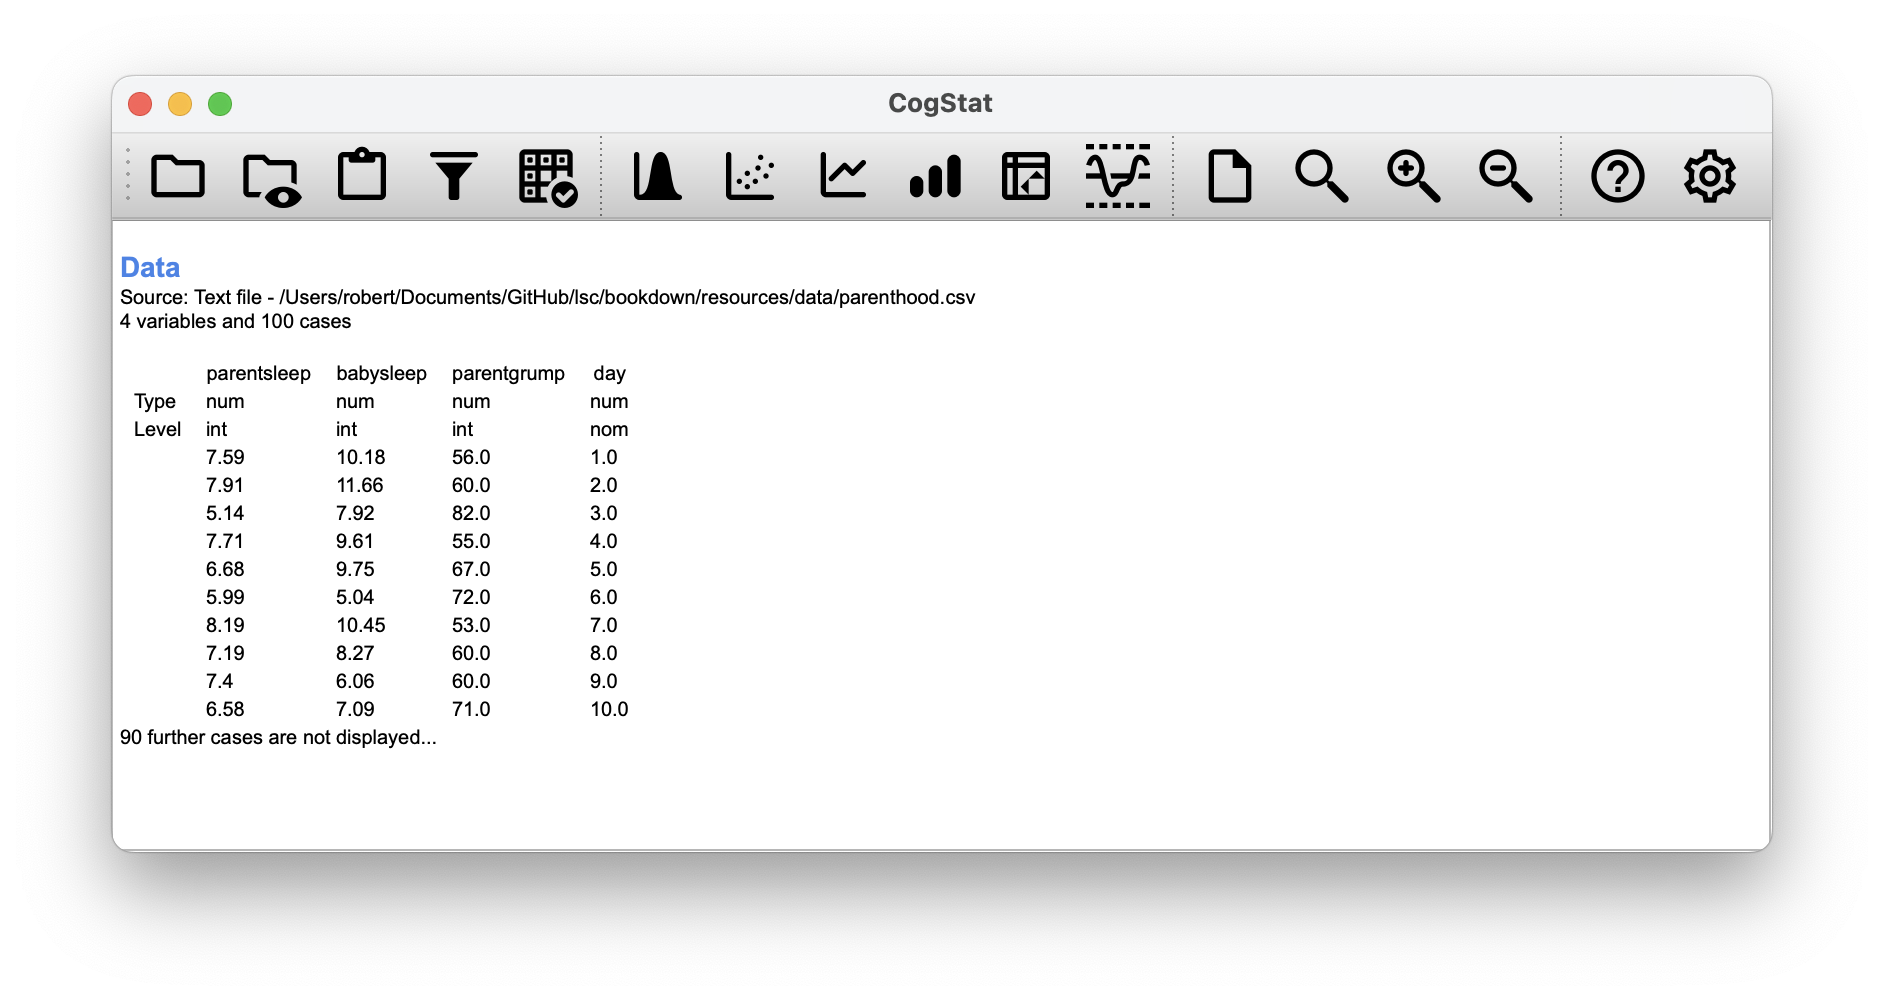
\includegraphics[width=0.66\linewidth]{resources/image/cogstatparenthoodload} 

}

\caption{This is what you would see after loading the parenthood.csv dataset.}\label{fig:loadparenthood}
\end{figure}

As described in Chapter \ref{exploringavariable}, we can get all the necessary descriptive statistics for all the variables: \texttt{parentsleep}, \texttt{babysleep} and \texttt{grumpiness}. Let's summarise all these into a neat little table (Table \ref{tab:parenthoodtab}).

\begin{table}[H]

\caption{\label{tab:parenthoodtab}Descriptive statistics for the parenthood data.}
\centering
\resizebox{\linewidth}{!}{
\begin{tabu} to \linewidth {>{\raggedright}X>{\centering}X>{\centering}X>{\centering}X}
\toprule
\multicolumn{1}{c}{} & \multicolumn{1}{c}{Parent grumpiness} & \multicolumn{1}{c}{Parent's hours slept} & \multicolumn{1}{c}{Baby's hours slept} \\
\cmidrule(l{3pt}r{3pt}){2-2} \cmidrule(l{3pt}r{3pt}){3-3} \cmidrule(l{3pt}r{3pt}){4-4}
 & `parentgrump` & `parentsleep` & `babysleep`\\
\midrule
Mean & 63.7 & 6.965 & 8.049\\
Standard deviation & 10 & 1.011 & 2.064\\
Skewness & 0.4 & -0.296 & -0.024\\
Kurtosis & 0 & -0.649 & -0.613\\
Range & 50 & 4.16 & 8.82\\
Maximum & 91 & 9 & 12.07\\
Upper quartile & 71 & 7.74 & 9.635\\
Median & 62 & 7.03 & 7.95\\
Lower quartile & 57 & 6.292 & 6.425\\
Minimum & 41 & 4.84 & 3.25\\
\bottomrule
\end{tabu}}
\end{table}

To start understanding the relationship between a pair of variables, select \texttt{Explore\ relation\ of\ variable\ pair} so a pop-up appears. Move the name of the two variables you wish to analyse from \texttt{Available\ variables} to \texttt{Selected\ variables}, then click \texttt{OK}. In CogStat, we can run analysis on multiple variables at once by selecting them in the variable list. This will display all analysis results after each other sequentially. We'll be looking at sections called \emph{Sample properties} from the result sets.

\begin{center}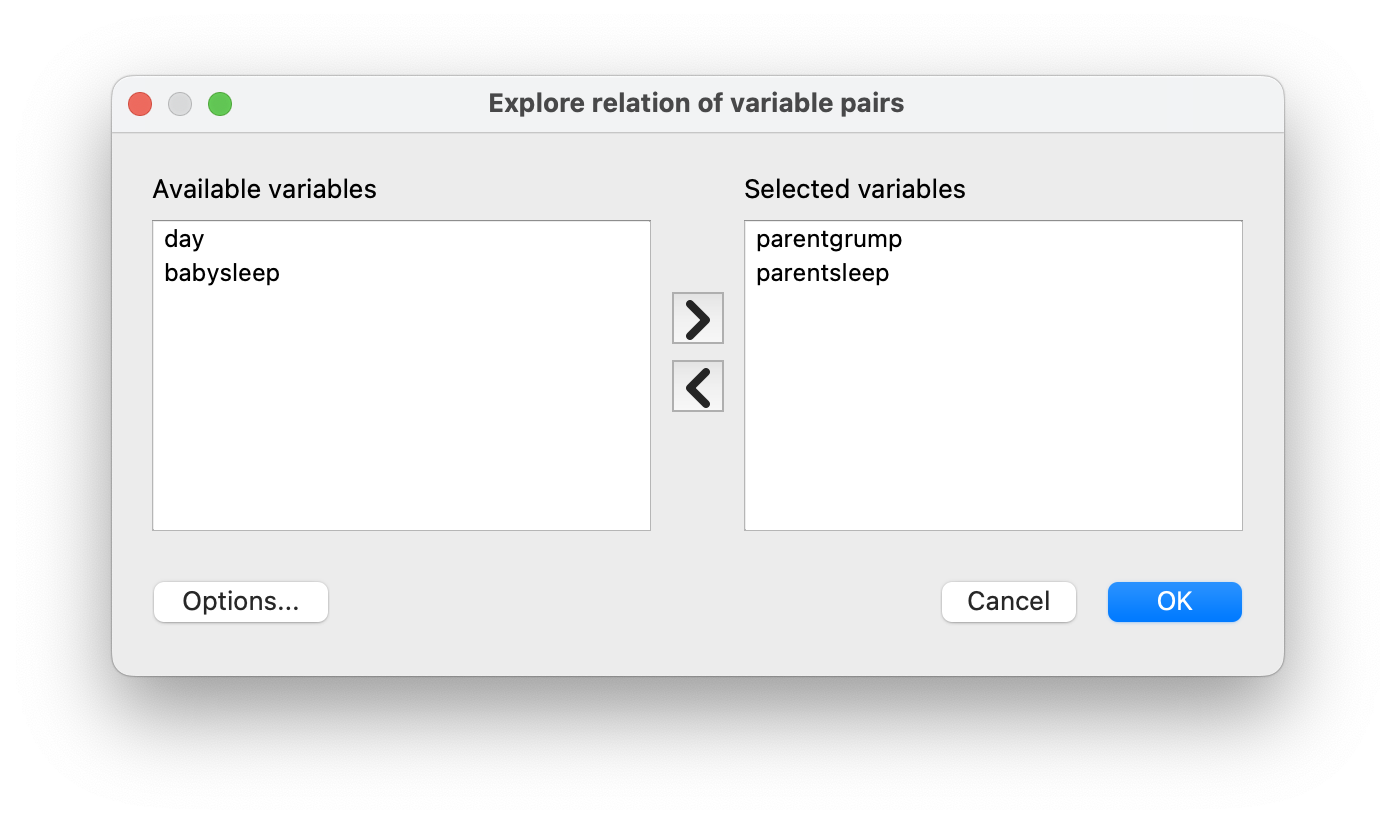
\includegraphics[width=0.66\linewidth]{resources/image/cogstatexplorevariablepair} \end{center}

\hypertarget{the-strength-and-direction-of-a-relationship}{%
\section{The strength and direction of a relationship}\label{the-strength-and-direction-of-a-relationship}}

We can draw scatterplots to give us a general sense of how closely related two variables are. Ideally, though, we might want to say a bit more about it than that. For instance, let's compare the relationship between \texttt{parentsleep} and \texttt{parentgrump} with that between \texttt{babysleep} and \texttt{parentgrump} (Figure \ref{fig:scatterparent1}).

\begin{figure}[h]

{\centering 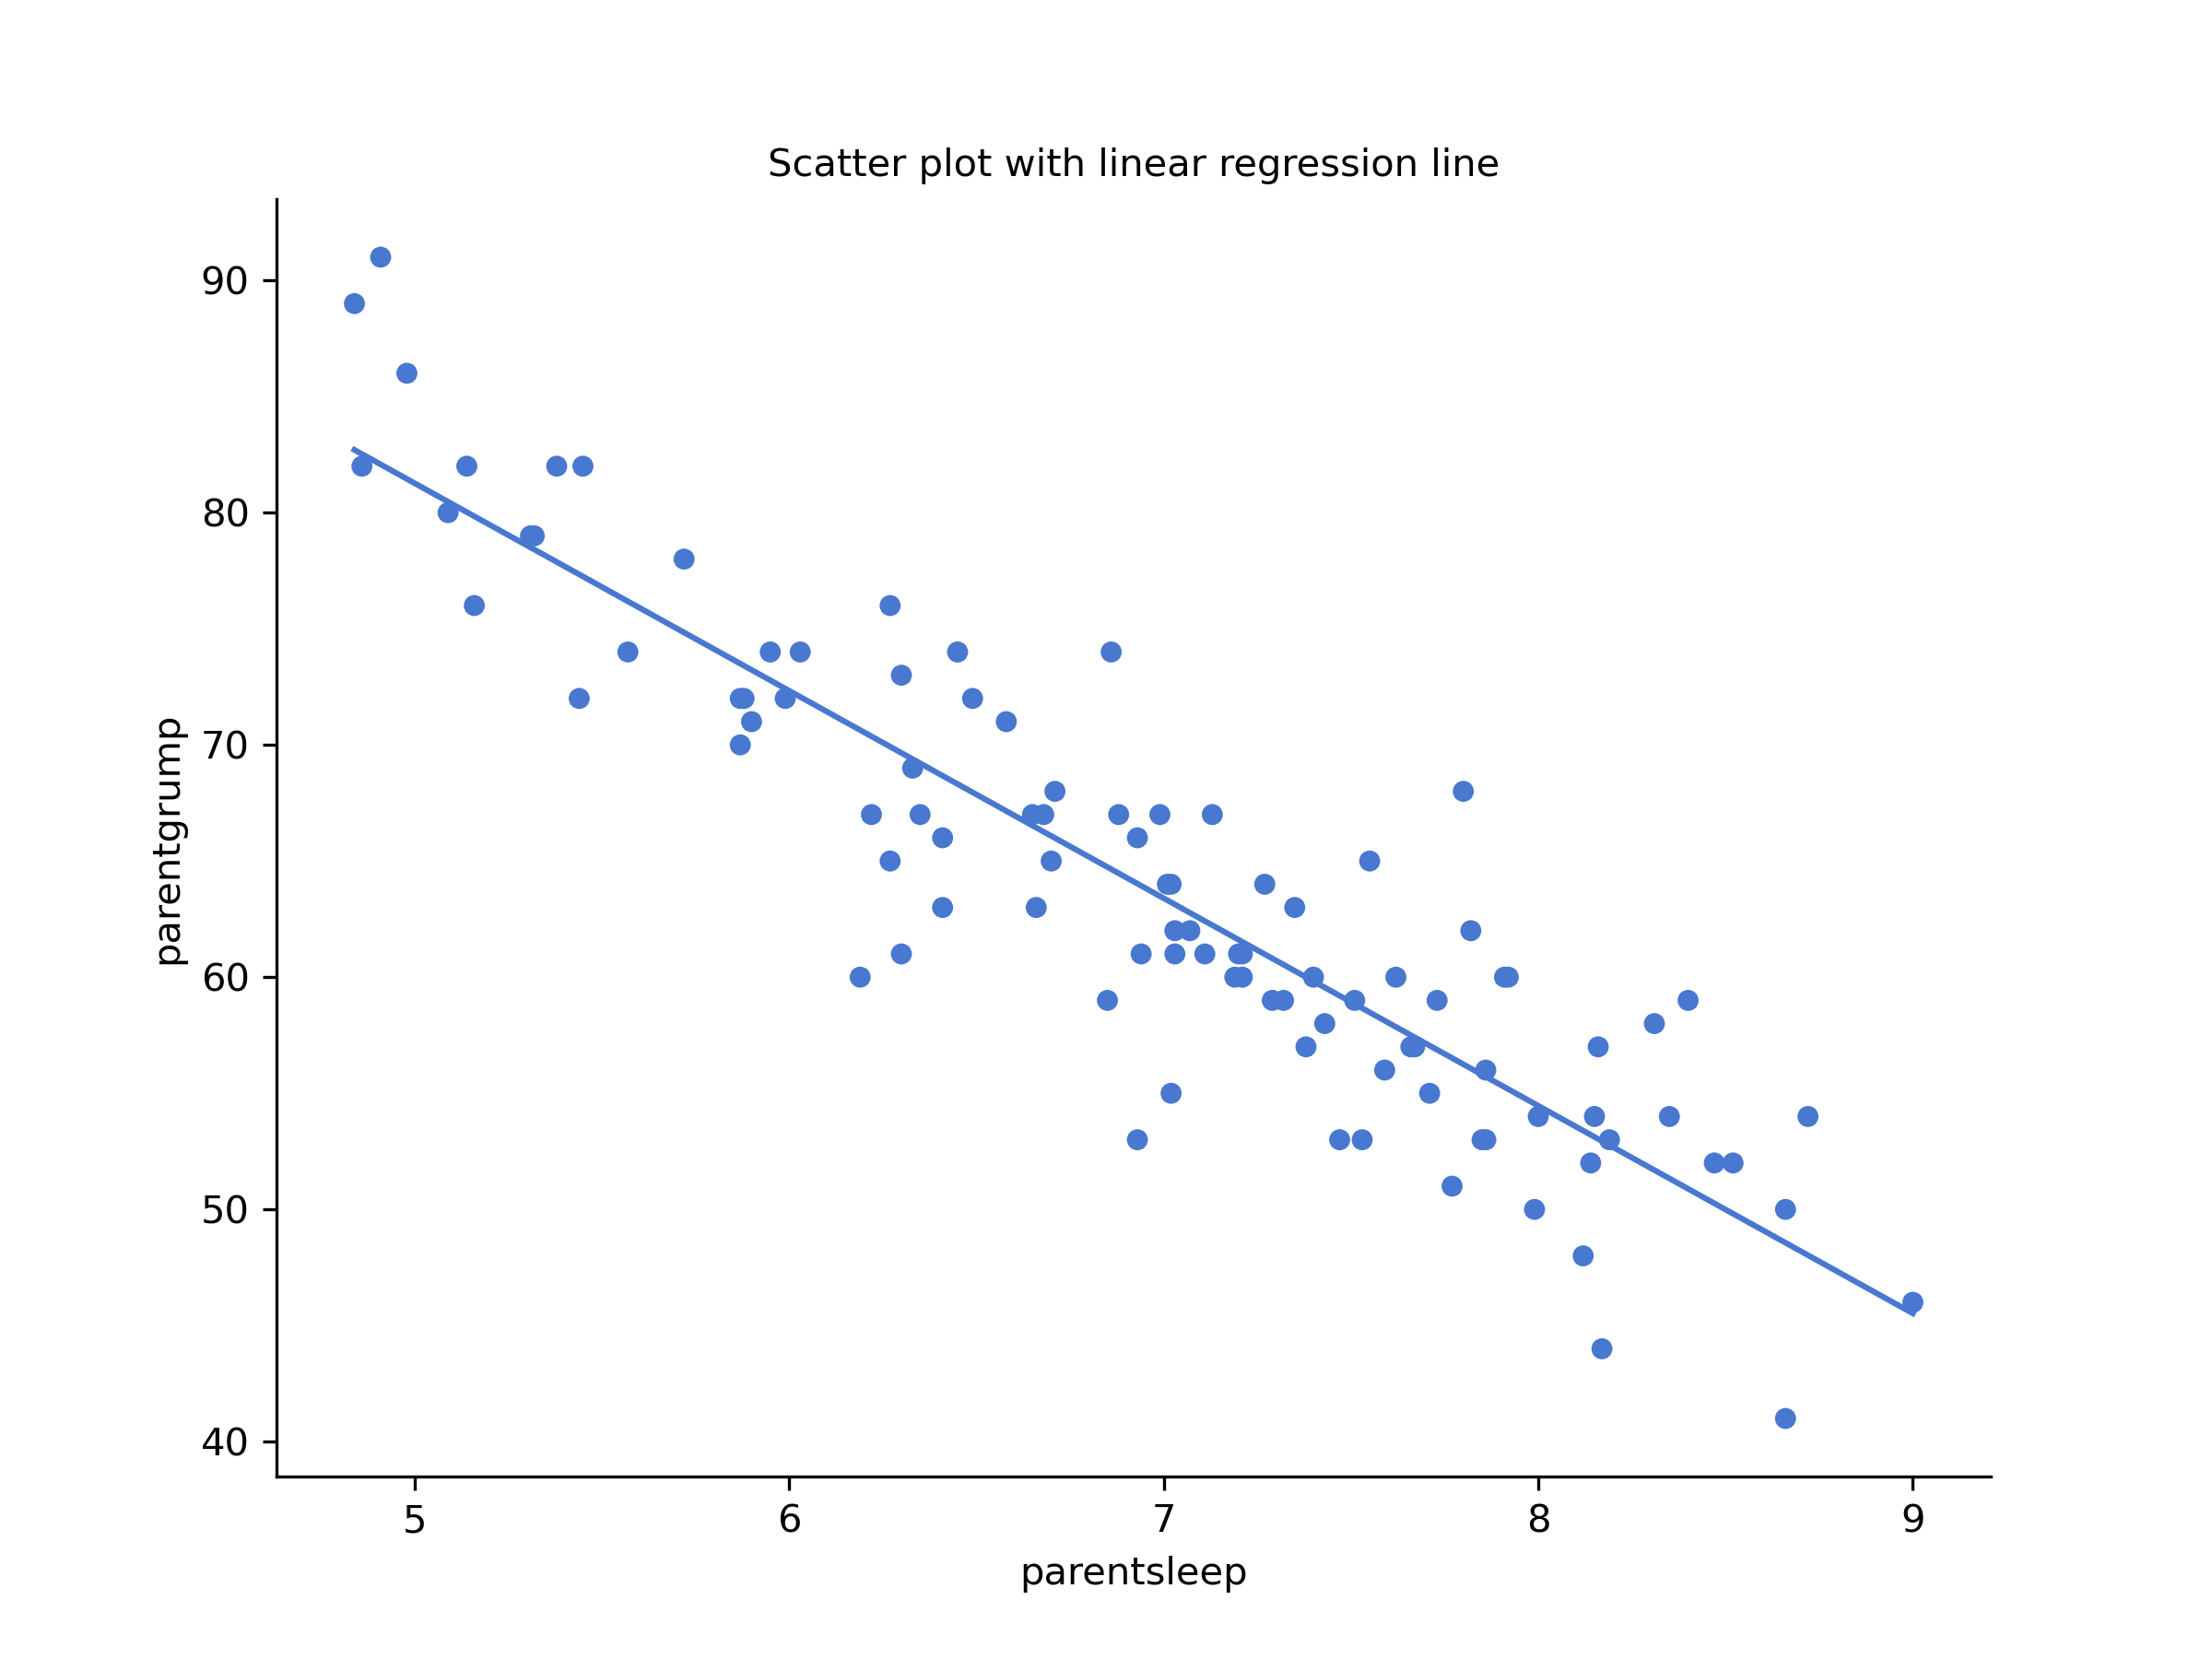
\includegraphics[width=0.45\linewidth]{resources/image/parentsleepgrumpplot} 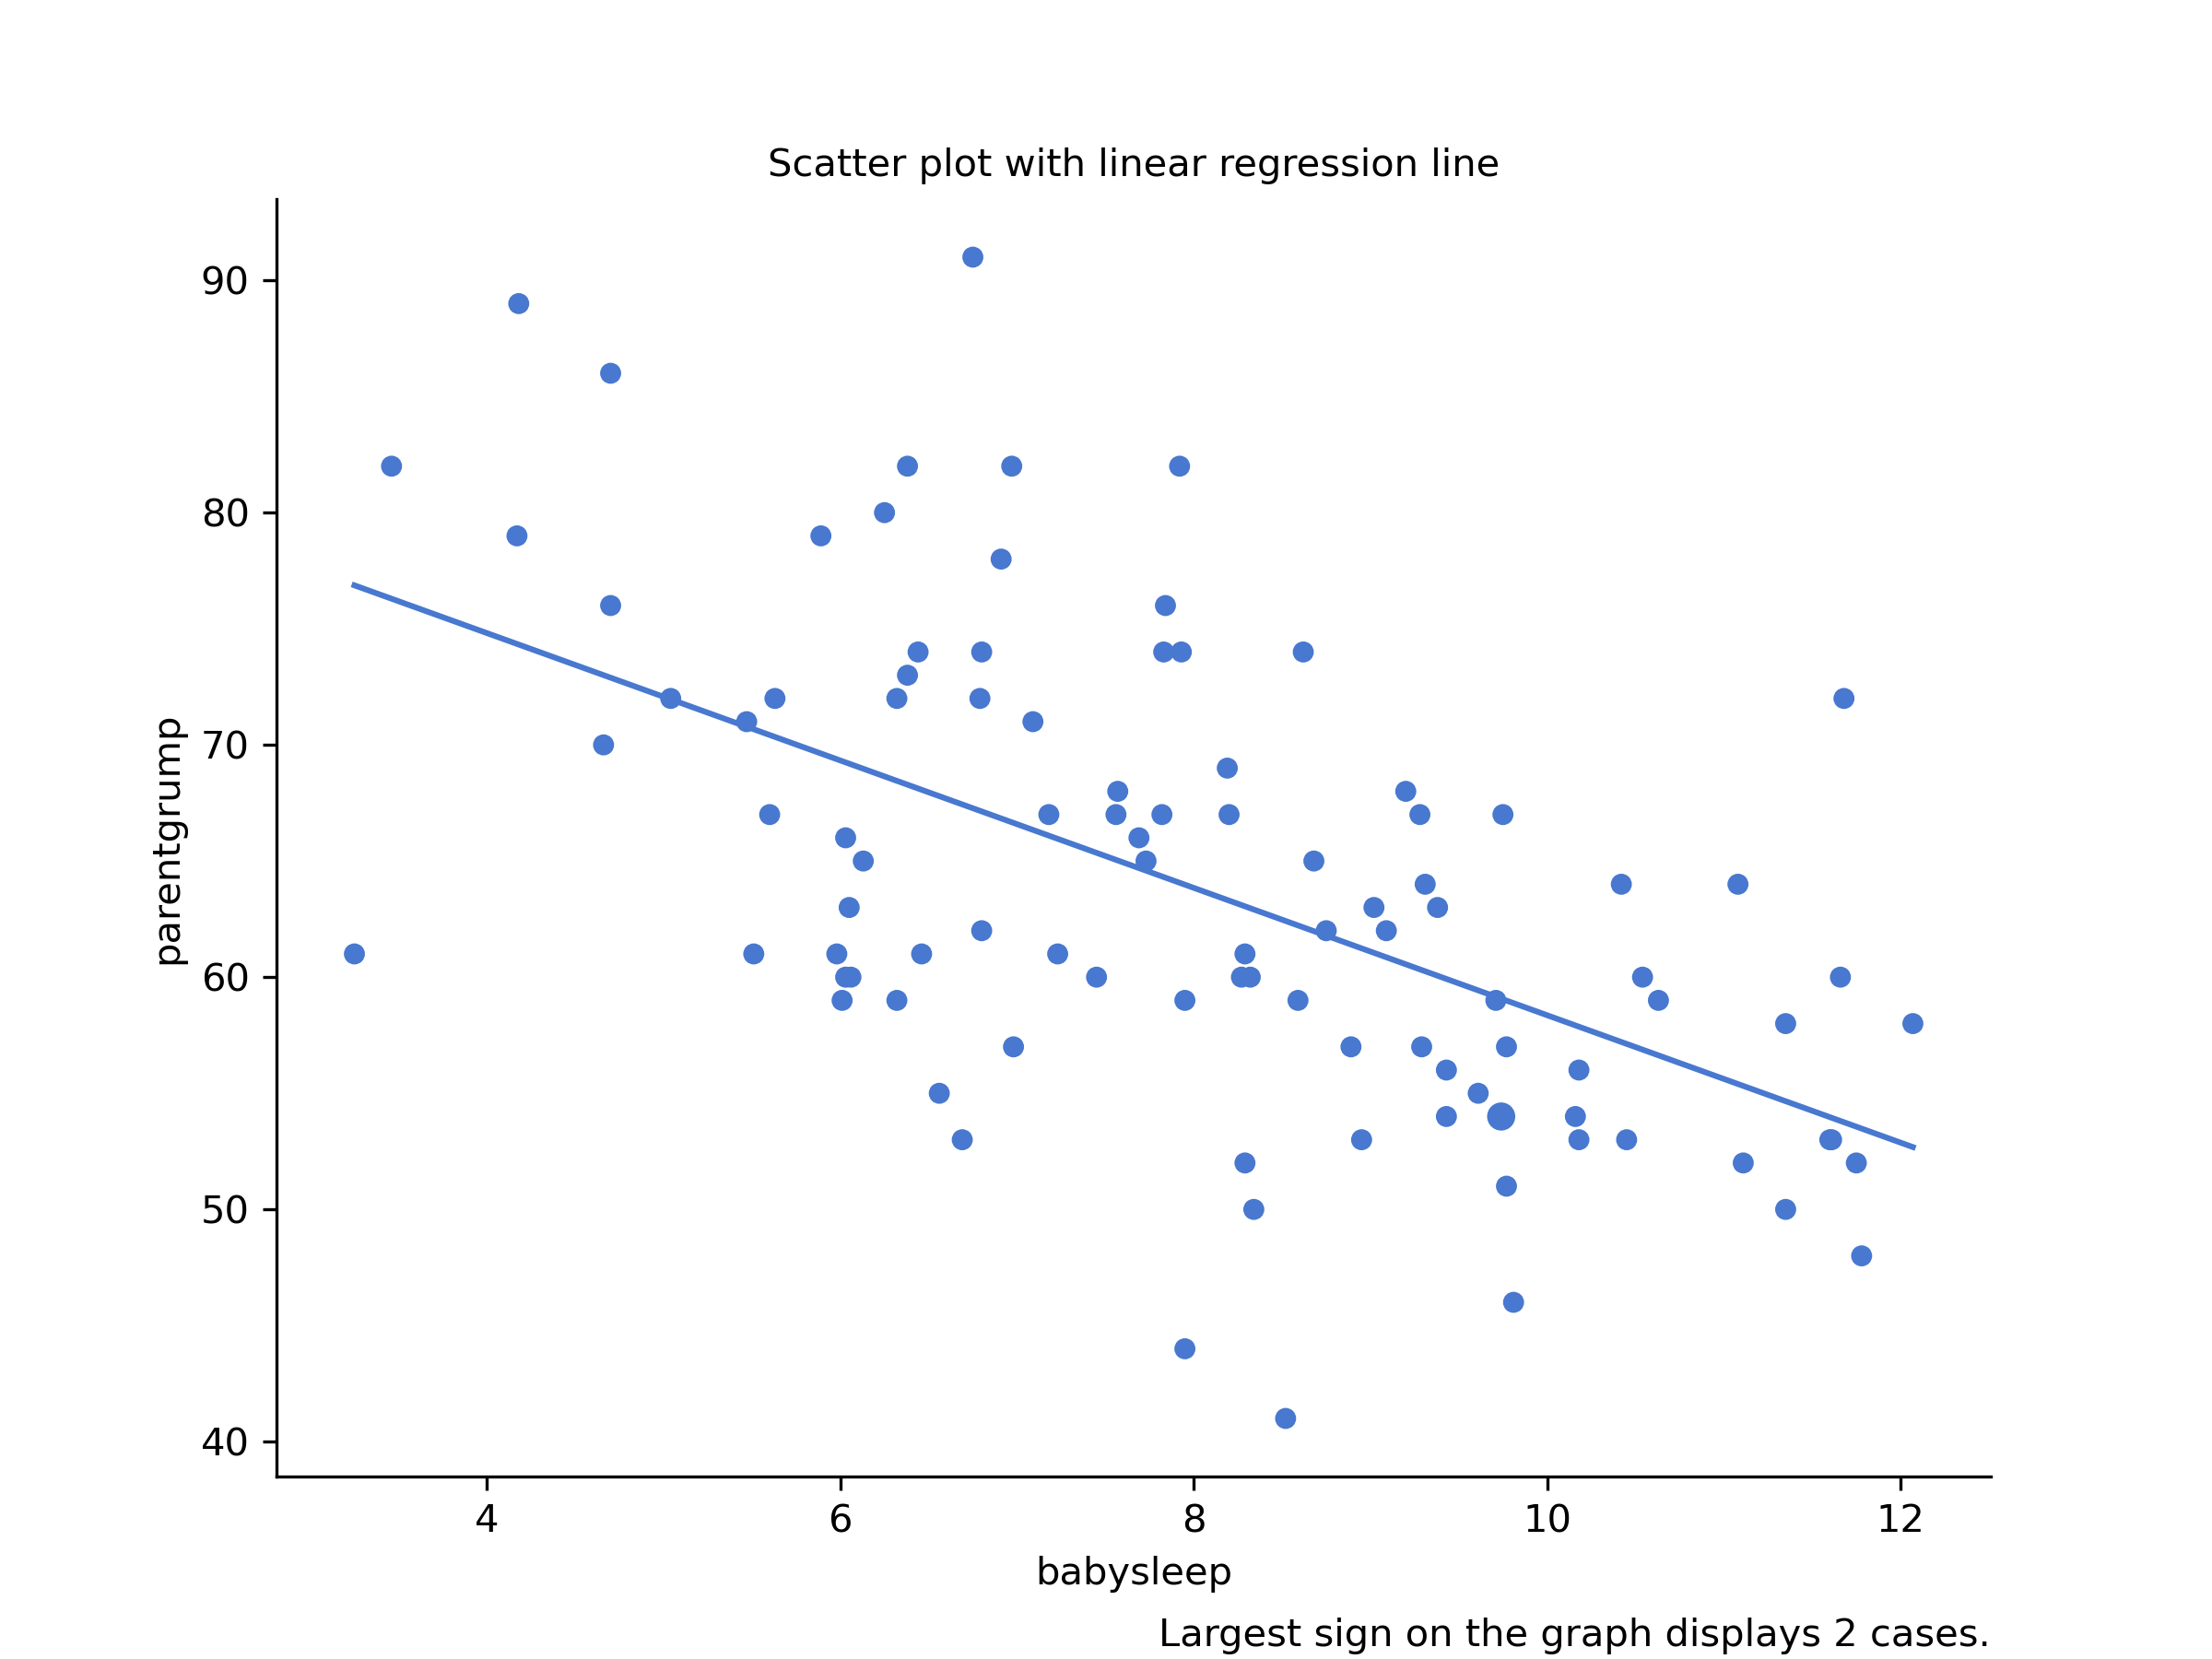
\includegraphics[width=0.45\linewidth]{resources/image/babysleepgrumpplot} 

}

\caption{Scatterplot drawn by CogStat showing the relationship between `parentsleep` and `parentgrump` and between `babysleep` and `parentgrump`}\label{fig:scatterparent1}
\end{figure}

When looking at these two plots side by side, it's clear that the relationship is \emph{qualitatively} the same in both cases: more sleep equals less grump! However, it's also obvious that the relationship between \texttt{parentsleep} and \texttt{parentgrump} is \emph{stronger} than between \texttt{babysleep} and \texttt{parentgrump}. The plot on the left is ``neater'' than on the right. It feels like if you want to predict the parent's mood, it will help you a little bit to know how many hours the baby slept, but it'd be \emph{more} helpful to know how many hours the parent slept.

\begin{callout}

\begin{callouttitle}
\textbf{Scatterplots}

\end{callouttitle}

\nopagebreak

On a scatterplot graph, each observation is represented by one dot in a coordinate system. The horizontal location of the dot plots the value of the observation on one variable, and the vertical location displays its value on the other variable.

Scatterplots are used often:

\begin{itemize}
\tightlist
\item
  to visualise the relationship between two variables,
\item
  to identify trends, which can be further explored with regression analysis (see Chapter \ref{regression}),
\item
  and to detect outliers.
\end{itemize}

Scatterplots can only be used with \protect\hyperlink{continuousdiscrete}{\emph{continuous variables}}. If you have a \protect\hyperlink{continuousdiscrete}{\emph{discrete variable}}, you can use a boxplot instead (see Chapter \ref{boxplots}).

\end{callout}

In contrast, let's consider Figure \ref{fig:scatterparent1} vs.~Figure \ref{fig:scatterparent2}. If we compare the scatterplot of ``\texttt{babysleep} v \texttt{parentgrump}'' to the scatterplot of ```\texttt{babysleep} v \texttt{parentsleep}'', the overall strength of the relationship is the same, but the direction is different. If the baby sleeps more, the parent gets \emph{more} sleep (positive relationship, but if the baby sleeps more, then the parent gets \emph{less} grumpy (negative relationship).

\begin{figure}

{\centering 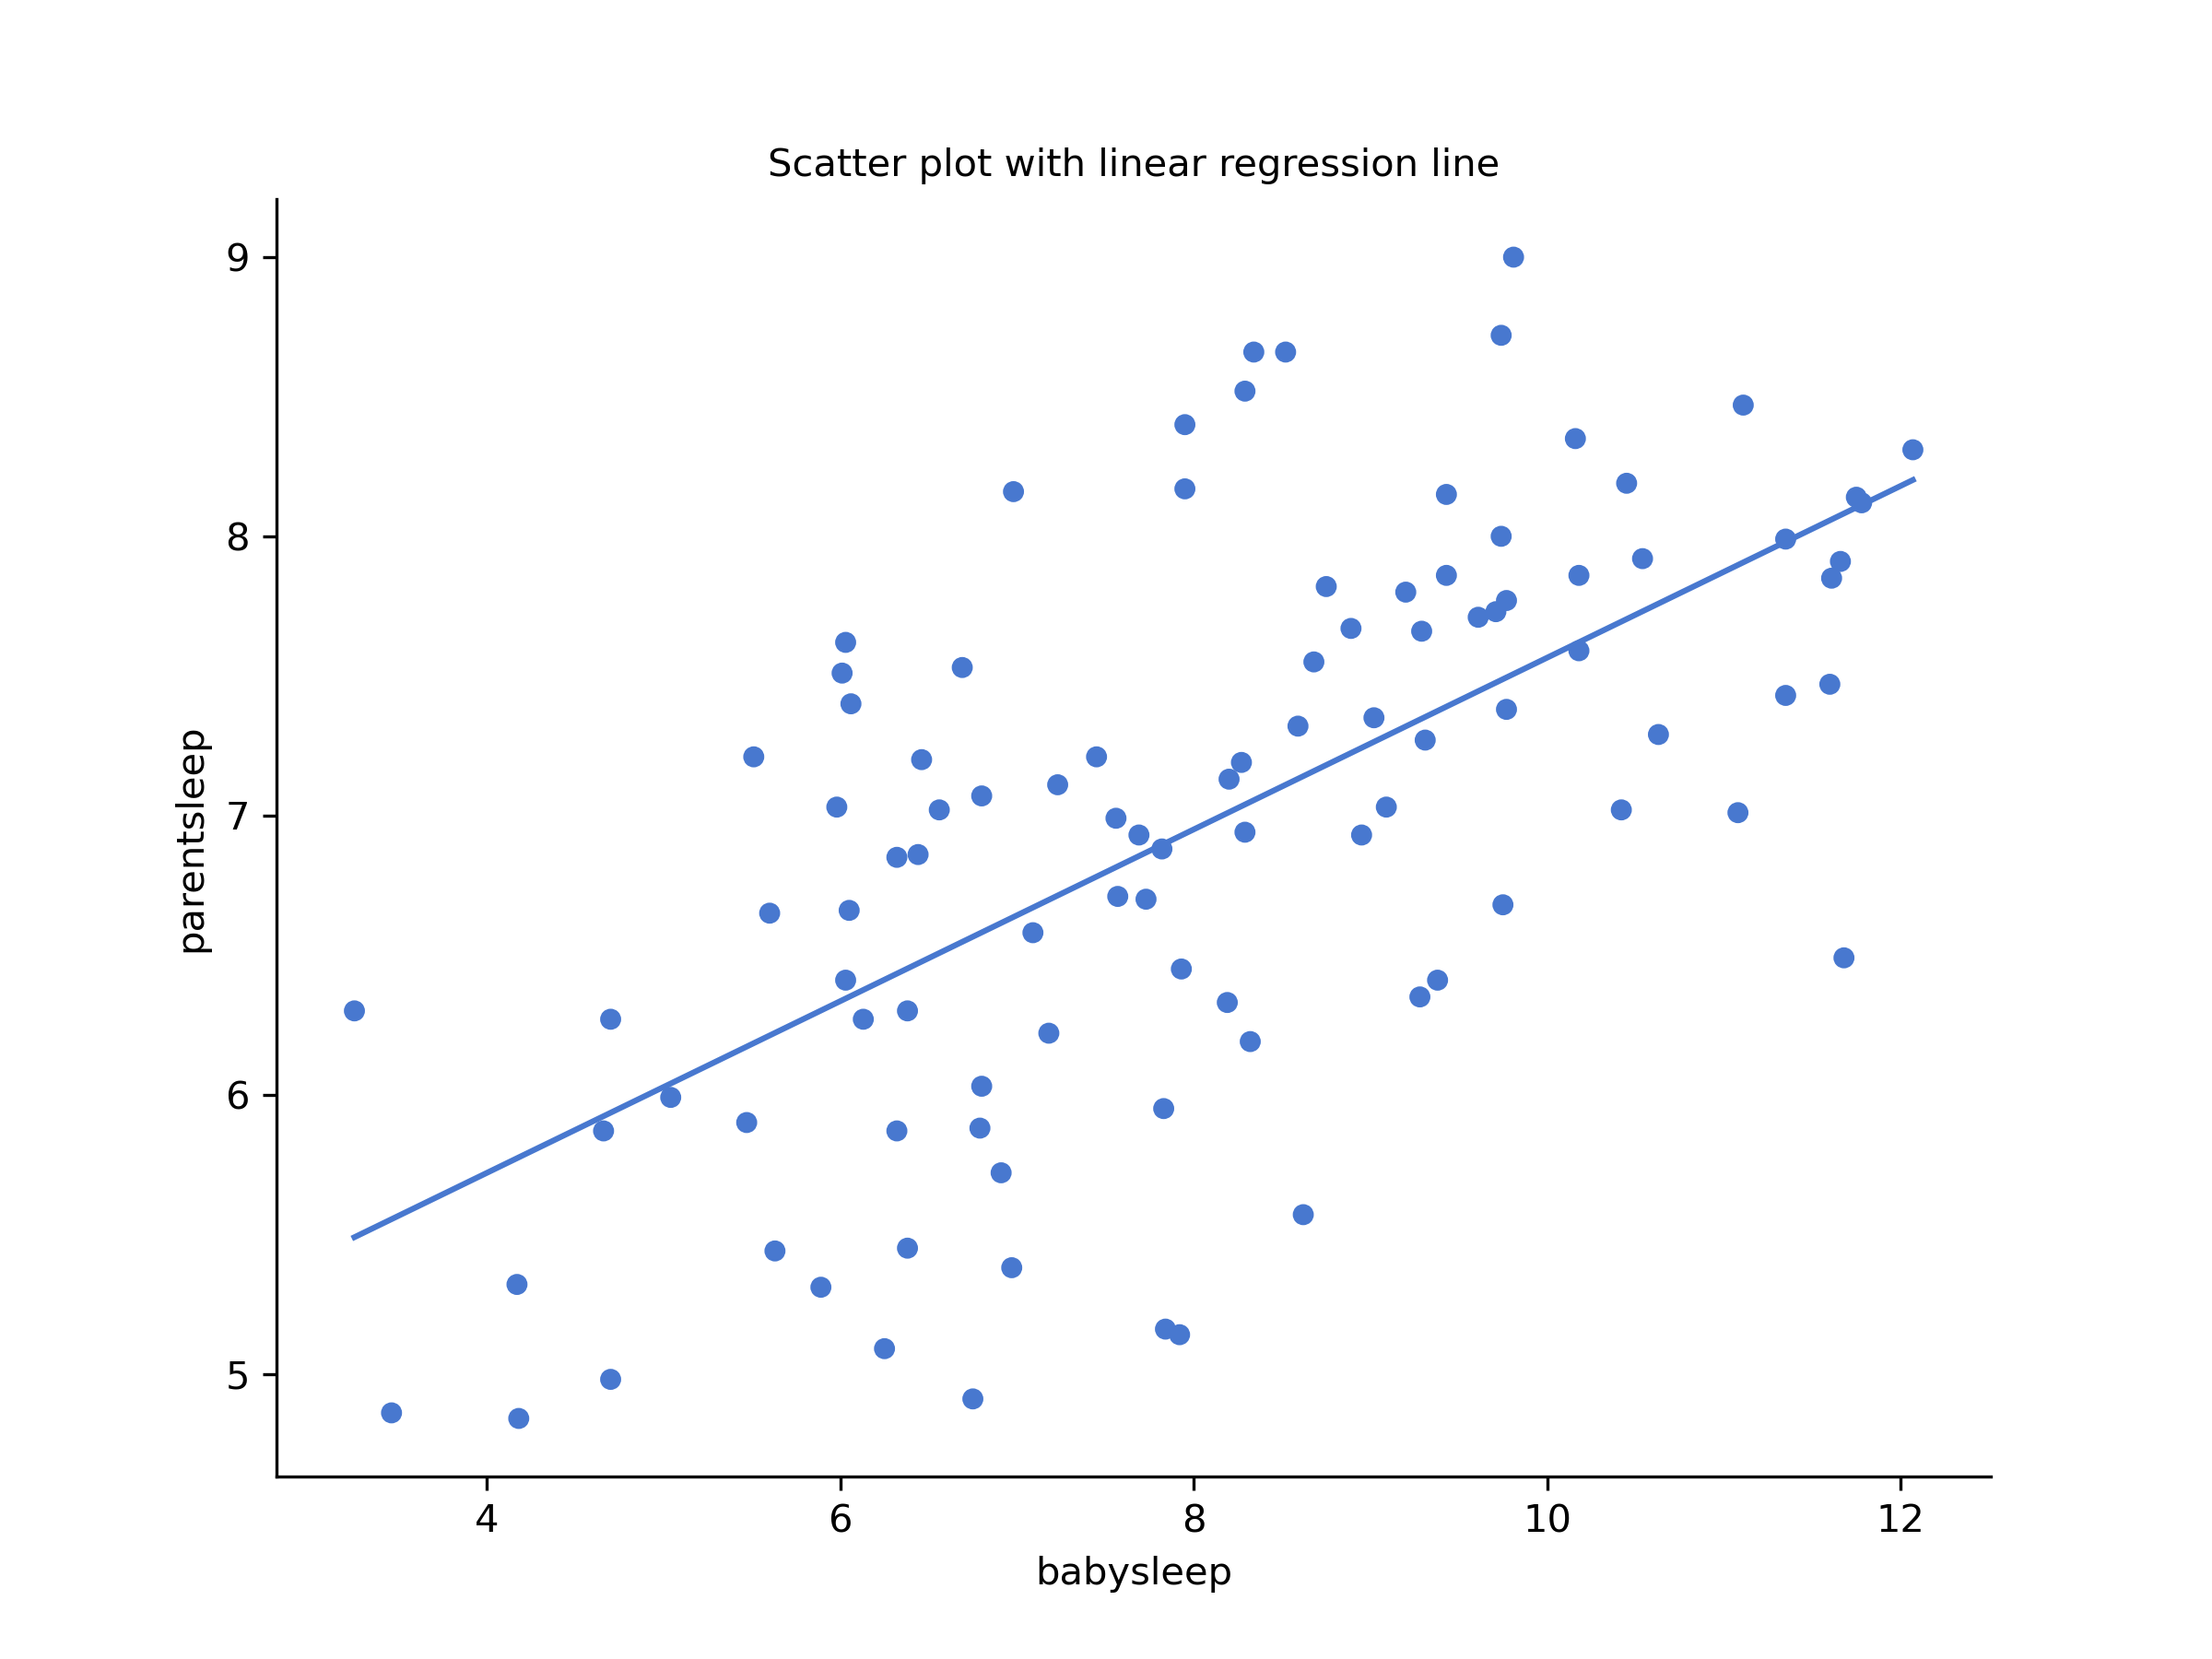
\includegraphics[width=0.66\linewidth]{resources/image/parentsleepbabysleepplot} 

}

\caption{Scatterplot drawn by CogStat showing the relationship between `babysleep` and `parentsleep`}\label{fig:scatterparent2}
\end{figure}

\hypertarget{pearson}{%
\section{The correlation coefficient}\label{pearson}}

We can make these ideas a bit more explicit by introducing the idea of a \textbf{correlation coefficient} (or, more specifically, \textbf{Pearson's correlation coefficient}), which is traditionally denoted by \(r\). The correlation coefficient between two variables \(X\) and \(Y\) (sometimes denoted \(r_{XY}\)), which we'll define more precisely shortly, is a measure that varies from \(-1\) to \(1\). When \(r = -1\), it means that we have a perfect negative relationship, and when \(r = 1\), it means we have a perfect positive relationship. When \(r = 0\), there's no relationship at all. If you look at Figure \ref{fig:corr}, you can see several plots showing what different correlations visually look like.

\begin{figure}

{\centering 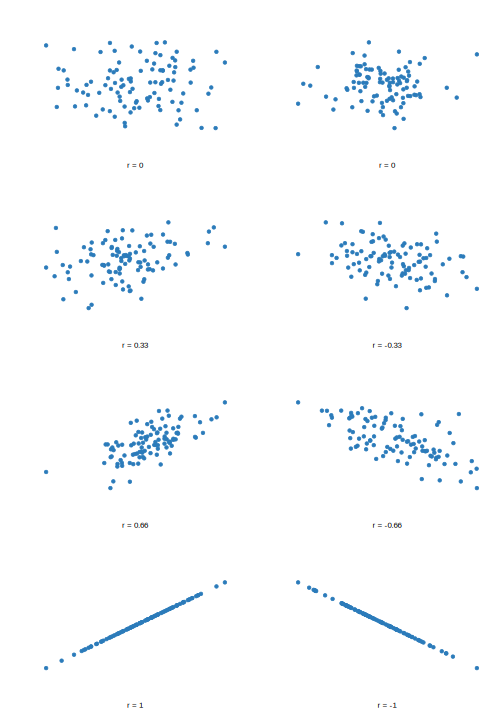
\includegraphics[width=0.66\linewidth]{lsc_files/figure-latex/corr-1} 

}

\caption{Illustration of the effect of varying the strength and direction of a correlation}\label{fig:corr}
\end{figure}

The Pearson's correlation coefficient formula can be written in several ways. The simplest way to write down the formula is to break it into two steps. Firstly, let's introduce the idea of a \textbf{covariance}. The covariance between two variables \(X\) and \(Y\) is a generalisation of the notion of the variance. It is a mathematically simple way of describing the relationship between two variables that isn't terribly informative to humans:
\[
\mbox{Cov}(X,Y) = \frac{1}{N-1} \sum_{i=1}^N \left( X_i - \bar{X} \right) \left( Y_i - \bar{Y} \right)
\]
Because we're multiplying (i.e., taking the ``product'' of) a quantity that depends on \(X\) by a quantity that depends on \(Y\) and then averaging\footnote{Just like we saw with the variance and the standard deviation, in practice, we divide by \(N-1\) rather than \(N\).}, you can think of the formula for the covariance as an ``average cross product'' between \(X\) and \(Y\). The covariance has the nice property that, if \(X\) and \(Y\) are entirely unrelated, the covariance is exactly zero. If the relationship between them is positive (in the sense shown in Figure \ref{fig:corr}), then the covariance is also positive. If the relationship is negative, then the covariance is also negative. In other words, the covariance captures the basic qualitative idea of correlation. Unfortunately, the raw magnitude of the covariance isn't easy to interpret: it depends on the units in which \(X\) and \(Y\) are expressed, and worse yet, the actual units in which the covariance is expressed are really weird. For instance, if \(X\) refers to the \texttt{parentsleep} variable (units: hours) and \(Y\) refers to the \texttt{parentgrump} variable (units: grumps), then the units for their covariance are ``hours \(\times\) grumps''. And I have no freaking idea what that would even mean.

The Pearson correlation coefficient \(r\) fixes this interpretation problem by standardising the covariance in the same way that the \(z\)-score standardises a raw score: dividing by the standard deviation. However, because we have two variables that contribute to the covariance, the standardisation only works if we divide by both standard deviations.\footnote{This is an oversimplification.} In other words, the correlation between \(X\) and \(Y\) can be written as follows:
\[
r_{XY} = \frac{\mbox{Cov}(X,Y)}{ \hat{\sigma}_X \ \hat{\sigma}_Y}
\]
By doing this standardisation, we keep all of the nice properties of the covariance discussed earlier, and the actual values of \(r\) are on a meaningful scale: \(r= 1\) implies a perfect positive relationship, and \(r = -1\) implies a perfect negative relationship.

\hypertarget{interpretingcorrelations}{%
\section{Interpreting a correlation}\label{interpretingcorrelations}}

Naturally, in real life, you don't see many correlations of 1. So how should you interpret a correlation of, say \(r= .4\)? The honest answer is that it really depends on what you want to use the data for, and on how strong the correlations in your field tend to be. A friend of Danielle's in engineering once argued that any correlation less than \(.95\) is completely useless (he may have been exaggerating, even for engineering). On the other hand, there are real cases -- even in psychology -- where you should expect strong correlations. For instance, one of the benchmark data sets used to test theories of how people judge similarities is so clean that any theory that can't achieve a correlation of at least \(.9\) isn't deemed successful. However, when looking for (say) elementary intelligence correlates (e.g., inspection time, response time), if you get a correlation above \(.3\) you're doing very well. In short, the interpretation of a correlation depends a lot on the context. That said, the rough guide in Table \ref{tab:interpretingcorrelations} is fairly typical.

\begin{table}

\caption{\label{tab:interpretingcorrelations}Rough guide to interpreting correlations}
\centering
\begin{tabular}[t]{lcc}
\toprule
Correlation & Strength & Direction\\
\midrule
-1.0 to -0.9 & Very strong & Negative\\
-0.9 to -0.7 & Strong & Negative\\
-0.7 to -0.4 & Moderate & Negative\\
-0.4 to -0.2 & Weak & Negative\\
-0.2 to 0 & Negligible & Negative\\
0 to 0.2 & Negligible & Positive\\
0.2 to 0.4 & Weak & Positive\\
0.4 to 0.7 & Moderate & Positive\\
0.7 to 0.9 & Strong & Positive\\
0.9 to 1.0 & Very strong & Positive\\
\bottomrule
\end{tabular}
\end{table}

However, something that can never be stressed enough is that you should \emph{always} look at the scatterplot before attaching any interpretation to the data. A correlation might not mean what you think it means. The classic illustration of this is ``Anscombe's Quartet'' (\protect\hyperlink{ref-Anscombe1973}{Anscombe, 1973}), which is a collection of four data sets. Each data set has two variables, an \(X\) and a \(Y\). For all four data sets, the mean value for \(X\) is 9, and the mean for \(Y\) is 7.5. The standard deviations for all \(X\) variables are almost identical, as are the standard deviations for the \(Y\) variables. And in each case the correlation between \(X\) and \(Y\) is \(r = 0.816\).

You'd think that these four data sets would look pretty similar to one another. They do not. If we draw scatterplots of \(X\) against \(Y\) for all four variables, as shown in Figure \ref{fig:anscombe} we see that all four of these are \emph{spectacularly} different to each other.

\begin{figure}

{\centering 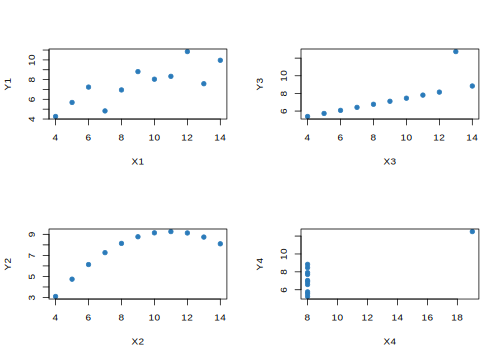
\includegraphics[width=0.66\linewidth]{lsc_files/figure-latex/anscombe-1} 

}

\caption{Anscombe's quartet. All four of these data sets have a Pearson correlation of $r = .816$, but they are qualitatively different from one another.}\label{fig:anscombe}
\end{figure}

The lesson here, which so very many people seem to forget in real life, is ``\emph{always graph your raw data}''.

\hypertarget{spearman}{%
\section{Spearman's rank correlations}\label{spearman}}

\begin{figure}

{\centering 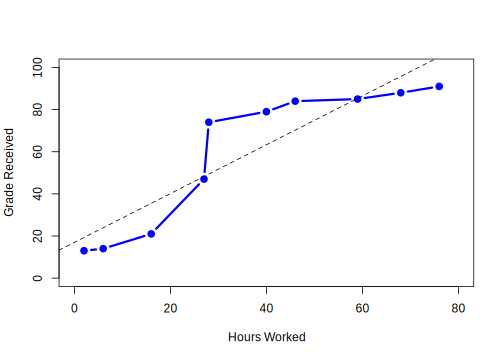
\includegraphics[width=0.66\linewidth]{lsc_files/figure-latex/rankcorrpic-1} 

}

\caption{The relationship between hours worked and grade received for a toy data set consisting of only 10 students (each circle corresponds to one student). The dashed line through the middle shows the linear relationship between the two variables. This produces a strong Pearson correlation of $r = .91$. However, the interesting thing to note here is that there's actually a perfect monotonic relationship between the two variables: in this toy example, at least, increasing the hours worked always increases the grade received, as illustrated by the solid line. This is reflected in a Spearman correlation of $rho = 1$. With such a small data set, however, it's an open question as to which version better describes the actual relationship involved.}\label{fig:rankcorrpic}
\end{figure}

The Pearson correlation coefficient is useful for many things, but it has shortcomings. One particular issue stands out: what it actually measures is the strength of the \emph{linear} relationship between two variables. In other words, it gives you a measure of the extent to which the data all tend to fall on a single, perfectly straight line. Often, this is a pretty good approximation to what we mean when we say ``relationship'', and so the Pearson correlation is a good thing to calculate. Sometimes, it isn't.

One very common situation where the Pearson correlation isn't quite the right thing to use arises when an increase in one variable \(X\) really is reflected in an increase in another variable \(Y\). However, the nature of the relationship isn't necessarily linear. An example of this might be the relationship between effort and reward when studying for an exam. If you put zero effort (\(X\)) into learning a subject, you should expect a grade of 0\% (\(Y\)). However, a little bit of effort will cause a \emph{massive} improvement: just turning up to lectures means that you learn a fair bit and if you just turn up to classes and scribble a few things down so your grade might rise to 35\%, all without a lot of effort. However, you just don't get the same effect at the other end of the scale. As everyone knows, it takes \emph{a lot} more effort to get a grade of 90\% than it takes to get a grade of 55\%. This means that if I've got data looking at study effort and grades, there's a good chance that Pearson correlations will be misleading.

To illustrate, consider the data plotted in Figure \ref{fig:rankcorrpic}, showing the relationship between hours worked and grade received for 10 students taking some classes. The curious thing about this -- highly fictitious -- data set is that increasing your effort \emph{always} increases your grade. It might be by a lot or by a little, but increasing the effort will never decrease your grade.

The data are stored in \href{resources/data/effort.csv}{\texttt{effort.csv}}. CogStat will calculate a standard Pearson correlation first\footnote{Unless, of course, you set your measurement level in the second row of the CSV as \texttt{"ord"} (\emph{ordinal}), because then you already tell the software that Pearson's \(r\) does not make sense to look at.}. It shows a strong relationship between hours worked and grade received: \(r = 0.909\). But this doesn't actually capture the observation that increasing hours worked \emph{always} increases the grade. There's a sense here in which we want to say that the correlation is \emph{perfect} but for a somewhat different notion of a ``relationship''. What we're looking for is something that captures the fact that there is a perfect \textbf{ordinal relationship} here. That is, if student 1 works more hours than student 2, then we can guarantee that student 1 will get a better grade. That's not what a correlation of \(r = 0.91\) says at all.

How should we address this? Actually, it's really easy: if we're looking for ordinal relationships, all we have to do is treat the data as if it were an ordinal scale! So, instead of measuring effort in terms of ``hours worked'', let us rank all 10 of our students in order of hours worked. That is, student 1 did the least work out of anyone (2 hours), so they got the lowest rank (rank = 1). Student 4 was the next laziest, putting in only 6 hours of work over the whole semester, so they got the next lowest rank (rank = 2). Notice that we're using ``rank = 1'' to mean ``low rank''. Sometimes in everyday language, we talk about ``rank = 1'' to mean ``top rank'' rather than ``bottom rank''. So be careful: you can rank ``from smallest value to largest value'' (i.e., small equals rank 1), or you can rank ``from largest value to smallest value'' (i.e., large equals rank 1). In this case, we're ranking from smallest to largest. But in real life, it's really easy to forget which way you set things up, so you have to put a bit of effort into remembering!

Okay, so let's have a look at our students when we rank them from worst to best in terms of effort and reward:

\begin{table}
\centering
\begin{tabular}{lcc}
\toprule
Student & Rank (hours worked) & Rank (grade received)\\
\midrule
student 1 & 1 & 1\\
student 2 & 10 & 10\\
student 3 & 6 & 6\\
student 4 & 2 & 2\\
student 5 & 3 & 3\\
student 6 & 5 & 5\\
student 7 & 4 & 4\\
student 8 & 8 & 8\\
student 9 & 7 & 7\\
student 10 & 9 & 9\\
\bottomrule
\end{tabular}
\end{table}

Hm. These are \emph{identical}. The student who put in the most effort got the best grade, the student with the least effort got the worst grade, etc. We can rank students by hours worked, then rank students by grade received, and these two rankings would be identical. So if we now correlate them, we get a perfect relationship: \(1\).

We've just re-invented the \textbf{Spearman's rank order correlation}, usually denoted \(\rho\) (pronounced: rho) to distinguish it from the Pearson correlation \(r\). CogStat will use \(r_{S}\) to denote rank order correlation.

CogStat will automatically calculate both Pearson's correlation and Spearman's rank order correlation for you if your measurement is not set in your source data (Figure \ref{fig:cogstatcorrelationresult}). If you set the measurement type to ``ordinal'' in your source file, it will omit to calculate Pearson's correlation due to the above reasons.

\begin{figure}

{\centering 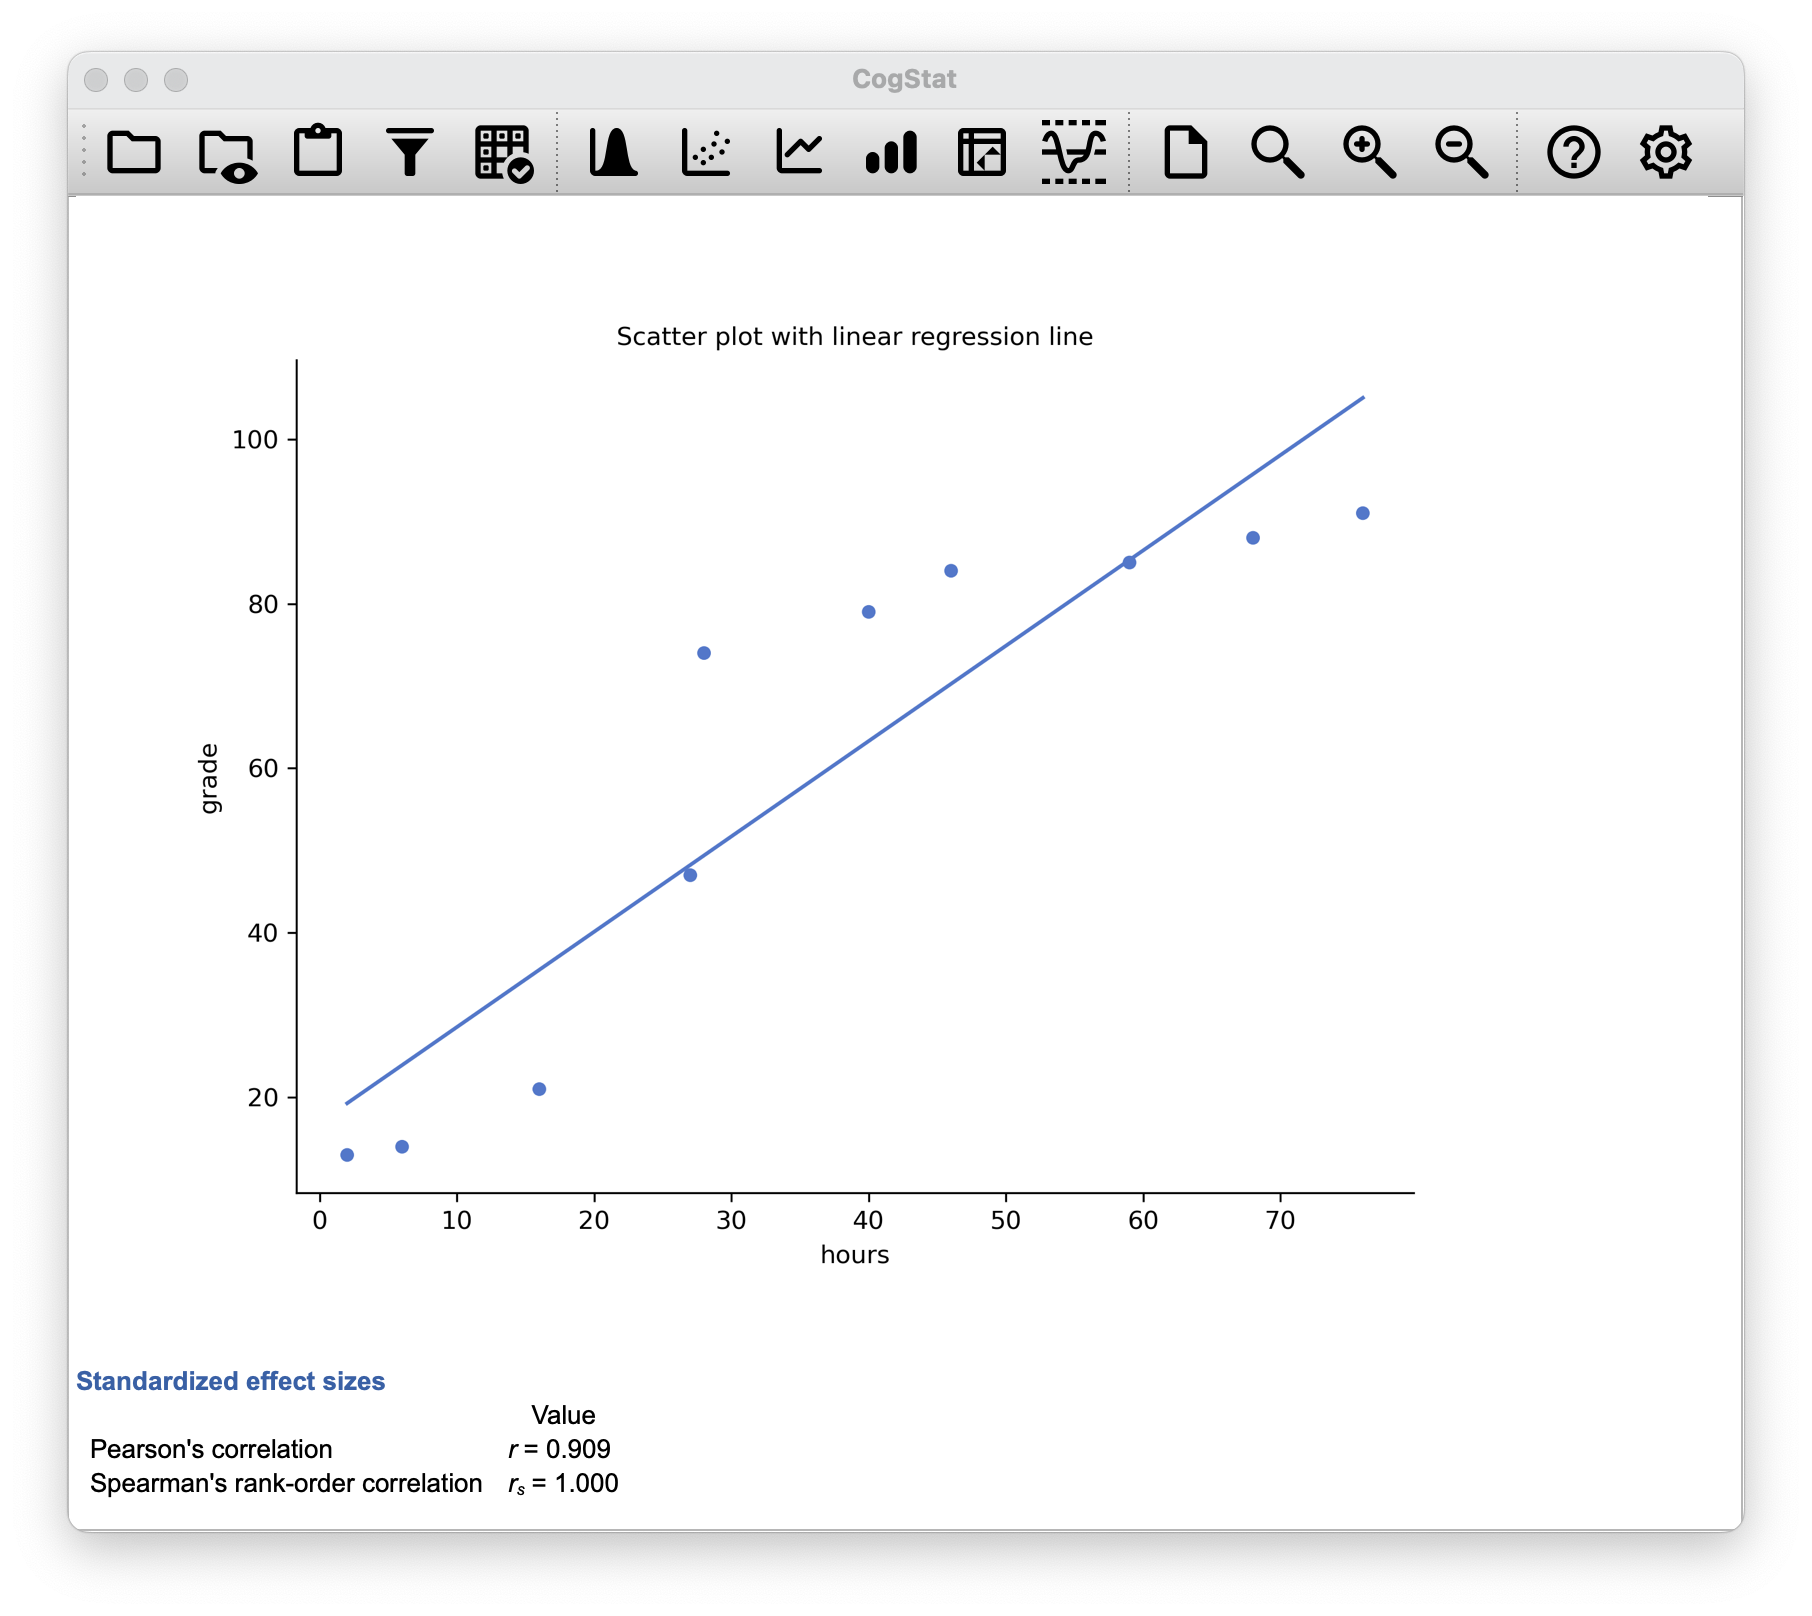
\includegraphics[width=0.66\linewidth]{resources/image/cogstatcorrelationresult} 

}

\caption{This is what you would see in CogStat after loading the `effort.csv` dataset.}\label{fig:cogstatcorrelationresult}
\end{figure}

\hypertarget{missingvaluespair}{%
\section{Missing values in pairwise calculations}\label{missingvaluespair}}

To illustrate the issues, let's open up a data set with missing values, \href{resources/data/parenthood_missing.csv}{\texttt{parenthood\_missing.csv}}. This file contains the same data as the original parenthood data but with some values deleted. While the original source could contain an empty value or \texttt{NA}, CogStat will display \texttt{NaN} for these missing values (Figure \ref{fig:parenthoodmissing}).

\begin{figure}

{\centering 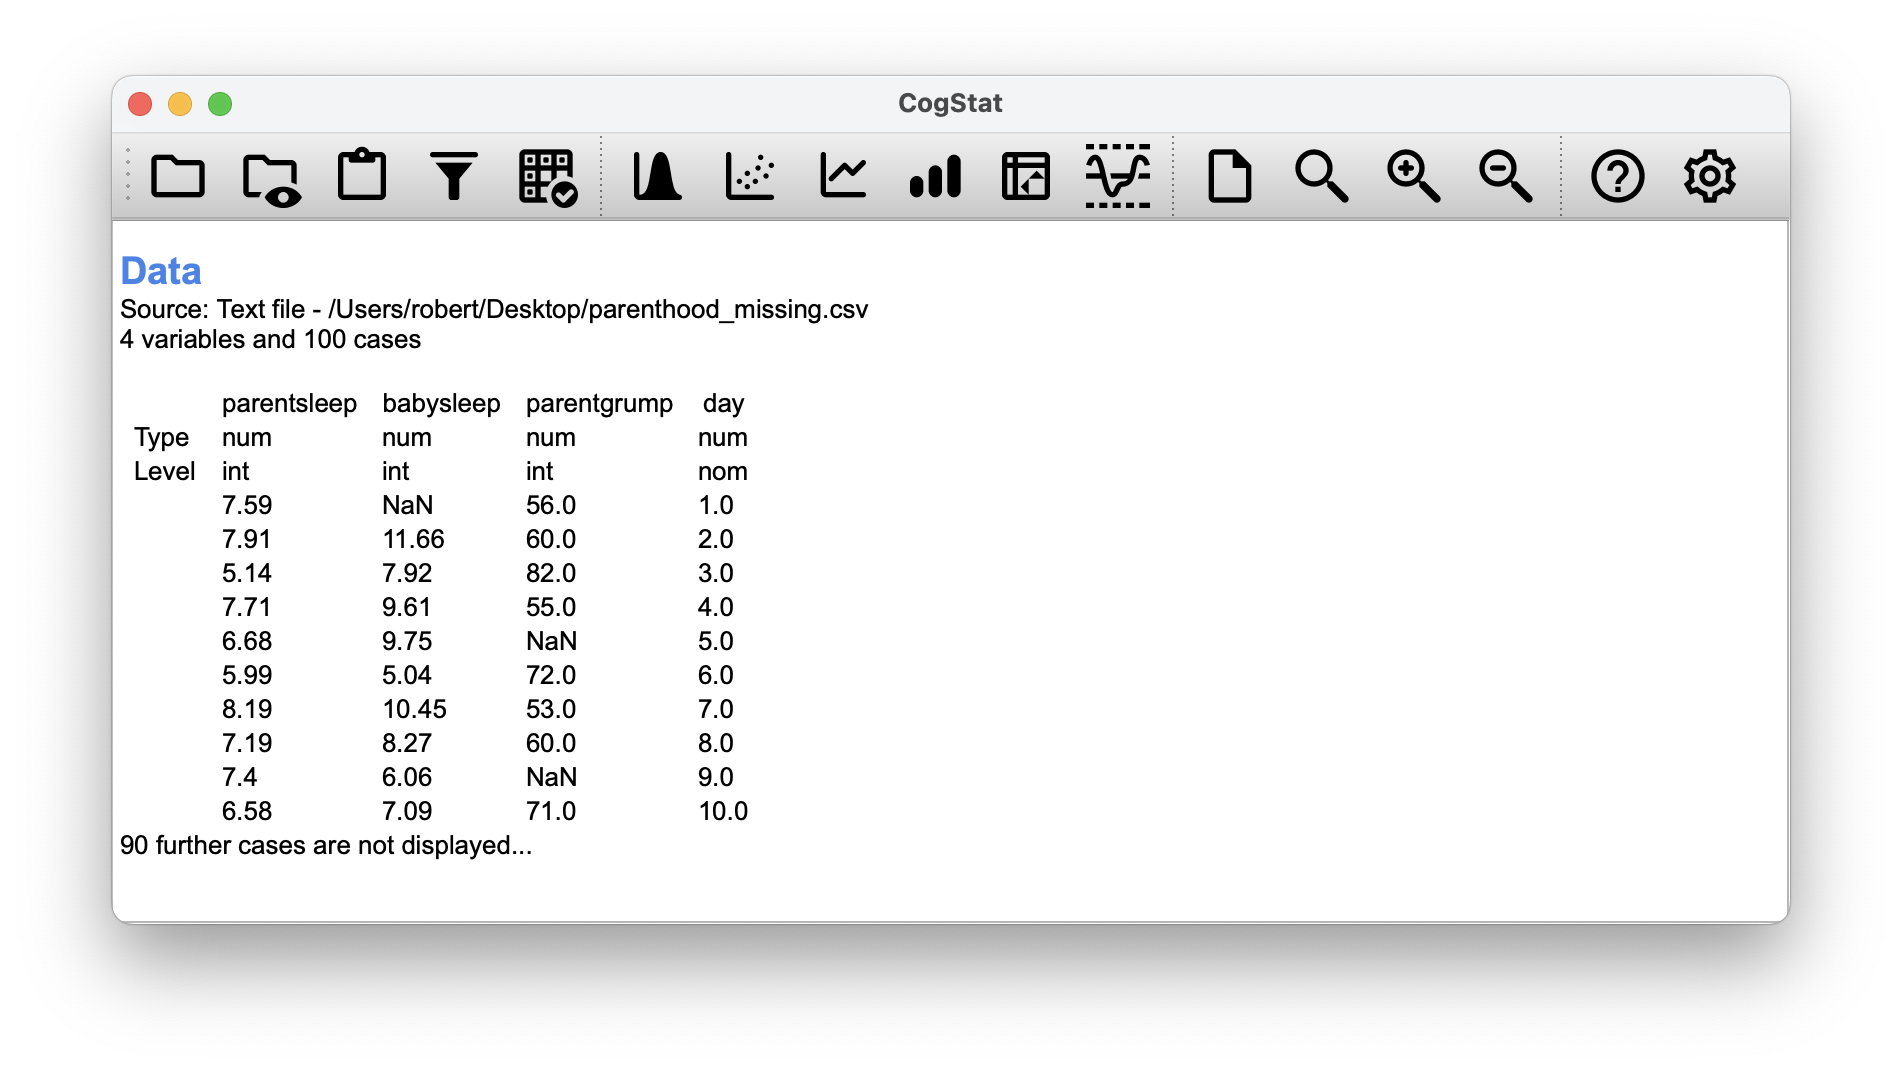
\includegraphics[width=0.66\linewidth]{resources/image/cogstatparenthood_missing} 

}

\caption{This is what you would see in CogStat after loading the adjusted dataset.}\label{fig:parenthoodmissing}
\end{figure}

Let's calculate descriptive statistics using the \texttt{Explore\ variable} function (See Chapter: \ref{exploringavariable}):

\begin{table}

\caption{\label{tab:parenthoodmissingtab}Descriptive statistics for the parenthood data with missing values. We can observe the slight difference in our statistics when we have missing values.}
\centering
\begin{tabular}[t]{lccc}
\toprule
\multicolumn{1}{c}{ } & \multicolumn{1}{c}{Parent grumpiness} & \multicolumn{1}{c}{Parent's hours slept} & \multicolumn{1}{c}{Baby's hours slept} \\
\cmidrule(l{3pt}r{3pt}){2-2} \cmidrule(l{3pt}r{3pt}){3-3} \cmidrule(l{3pt}r{3pt}){4-4}
  & `parentgrump` & `parentsleep` & `babysleep`\\
\midrule
Mean & 63.2 & 6.977 & 8.114\\
Standard deviation & 9.8 & 1.015 & 2.035\\
Skewness & 0.4 & -0.346 & -0.096\\
Kurtosis & -0.2 & -0.647 & -0.5\\
Range & 48 & 4.16 & 8.82\\
Maximum & 89 & 9 & 12.07\\
Upper quartile & 70.2 & 7.785 & 9.61\\
Median & 61 & 7.03 & 8.2\\
Lower quartile & 56 & 6.285 & 6.46\\
Minimum & 41 & 4.84 & 3.25\\
\bottomrule
\end{tabular}
\end{table}

We can see that there are 9 missing values for \texttt{parentsleep} (\texttt{N\ of\ missing\ cases:\ 9}), 11 missing values for \texttt{babysleep} (\texttt{N\ of\ missing\ cases:\ 11}), and 8 missing values for \texttt{parentgrump} (\texttt{N\ of\ missing\ cases:\ 8}).

Whichever pair you'd like to run (e.g., \texttt{parentsleep} vs.~\texttt{parentgrump}), CogStat will automatically exclude the missing values from the calculation:

\begin{figure}

{\centering 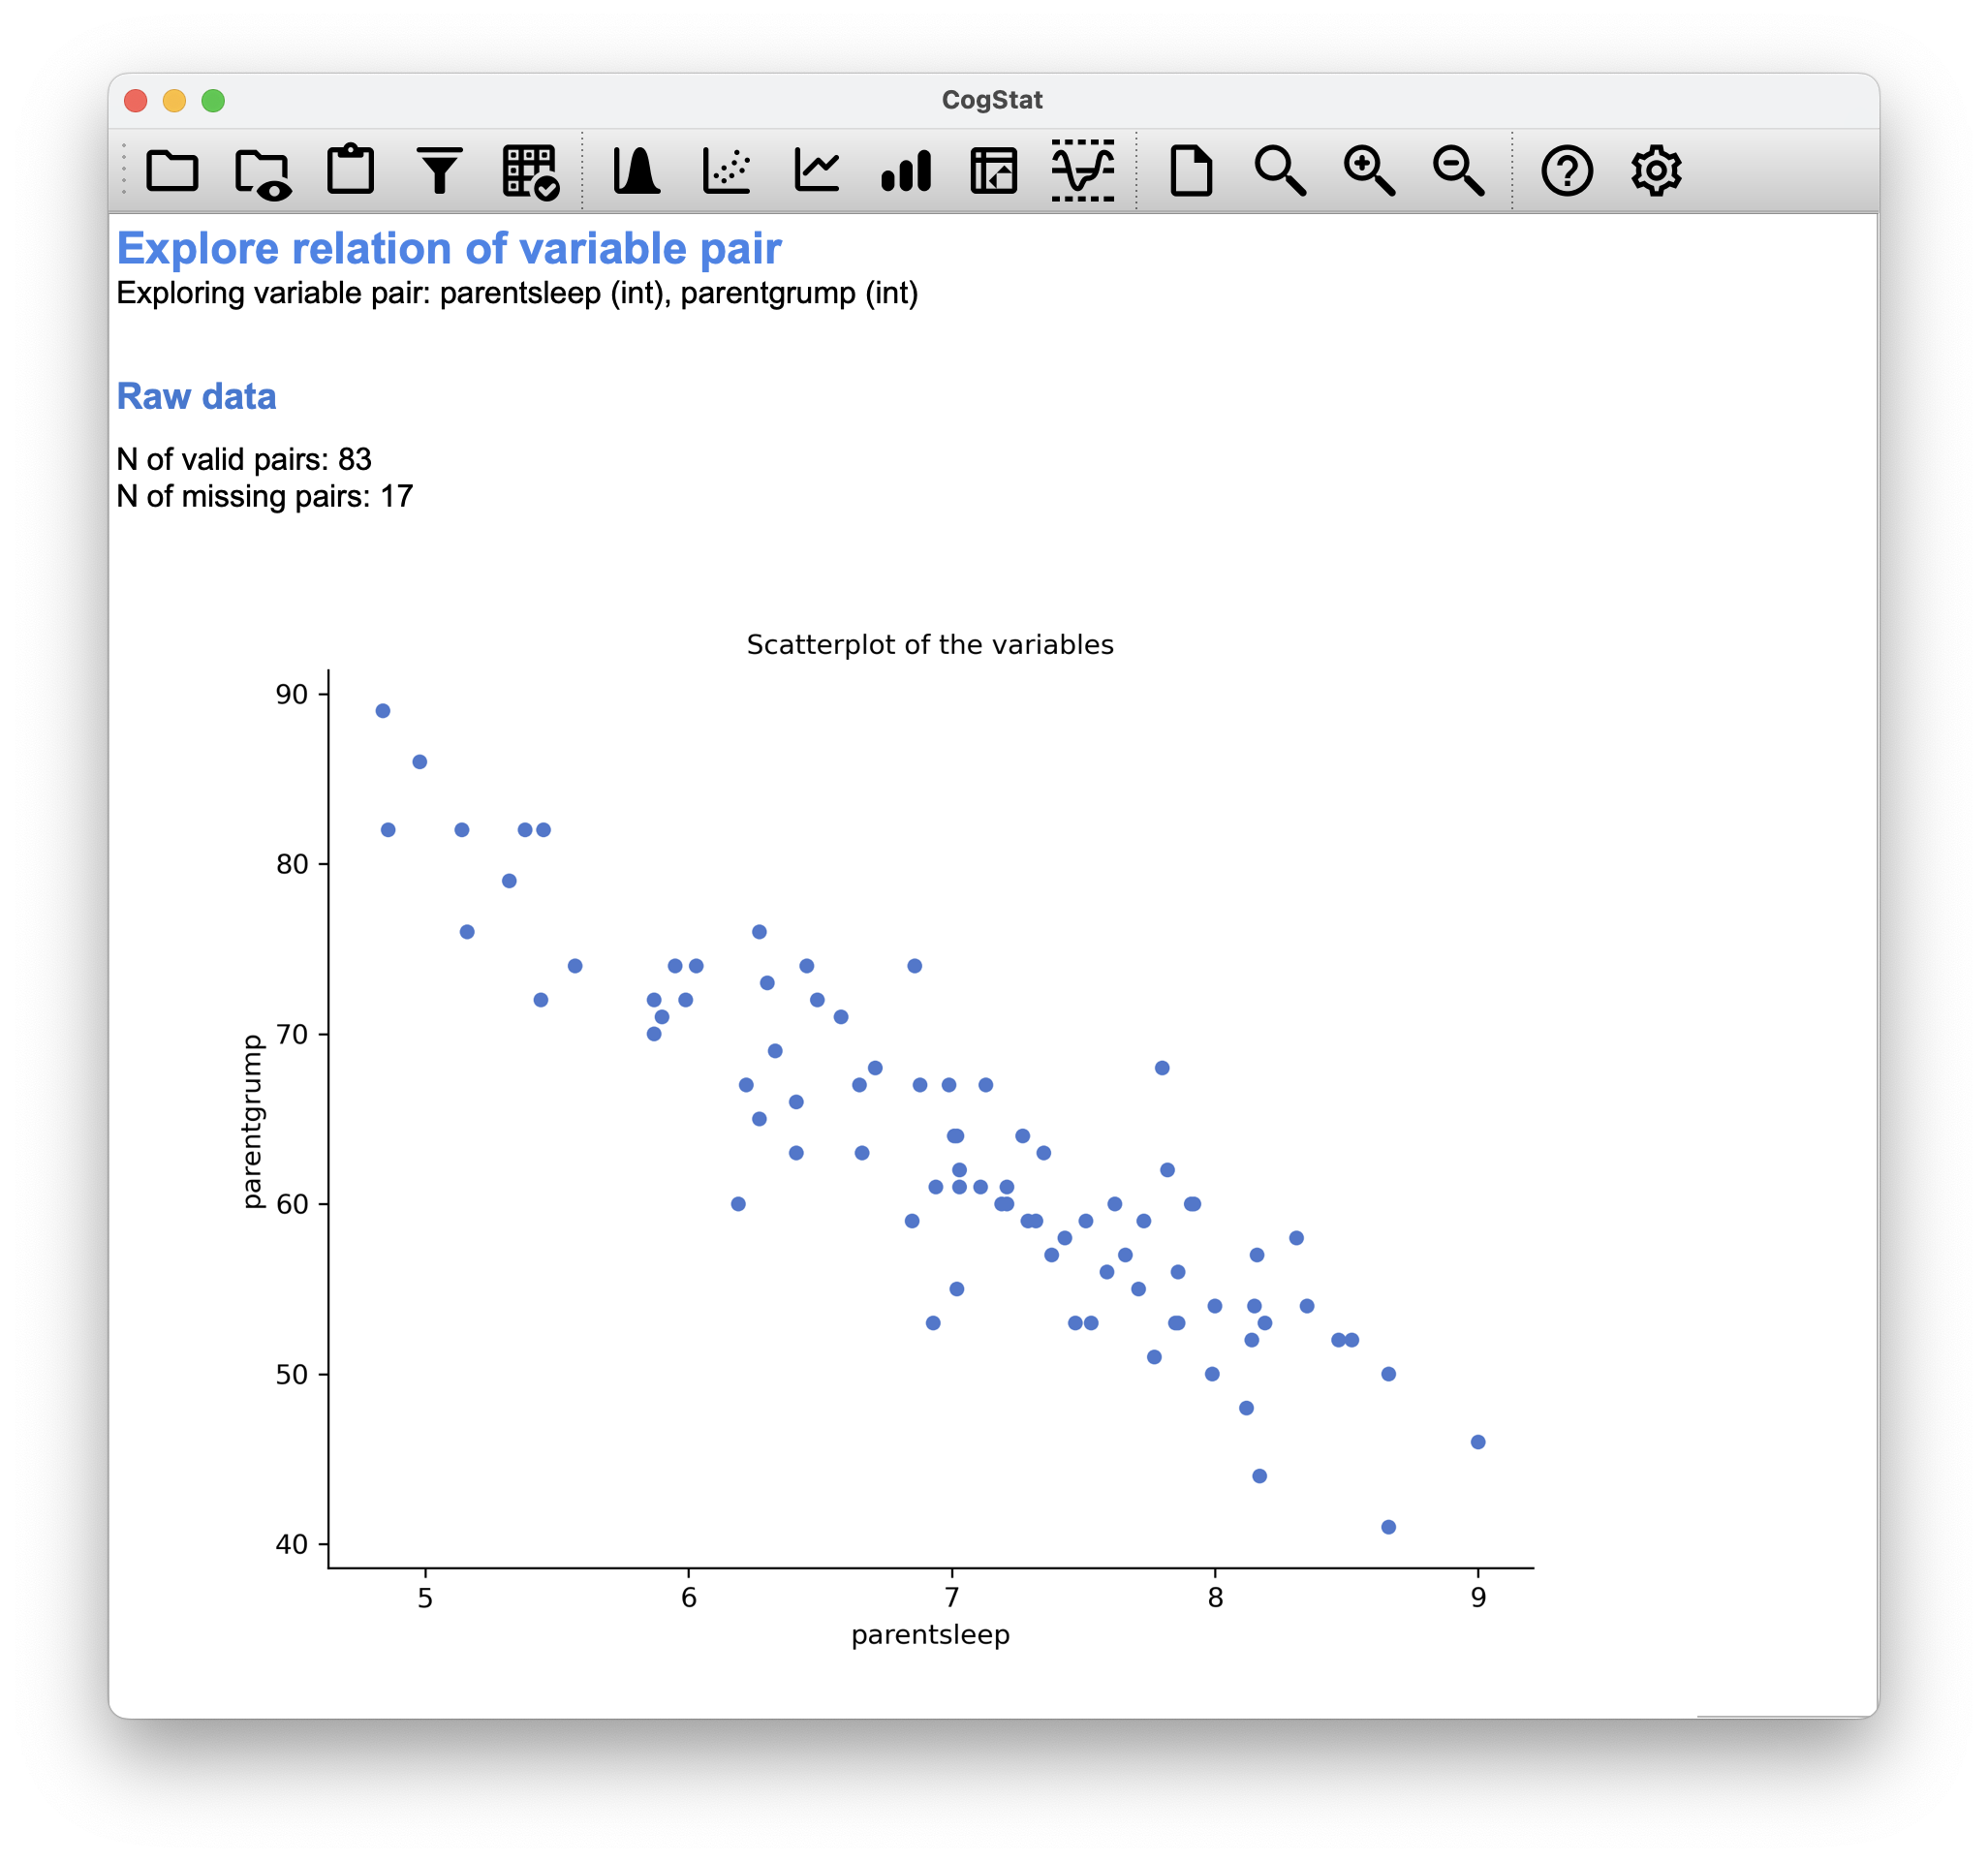
\includegraphics[width=0.66\linewidth]{resources/image/cogstatparentsleepparentgrumpmissing} 

}

\caption{17 missing pairs when comparing `parentsleep` and `parentgrump`}\label{fig:parenthoodmissingcog1}
\end{figure}

\begin{figure}

{\centering 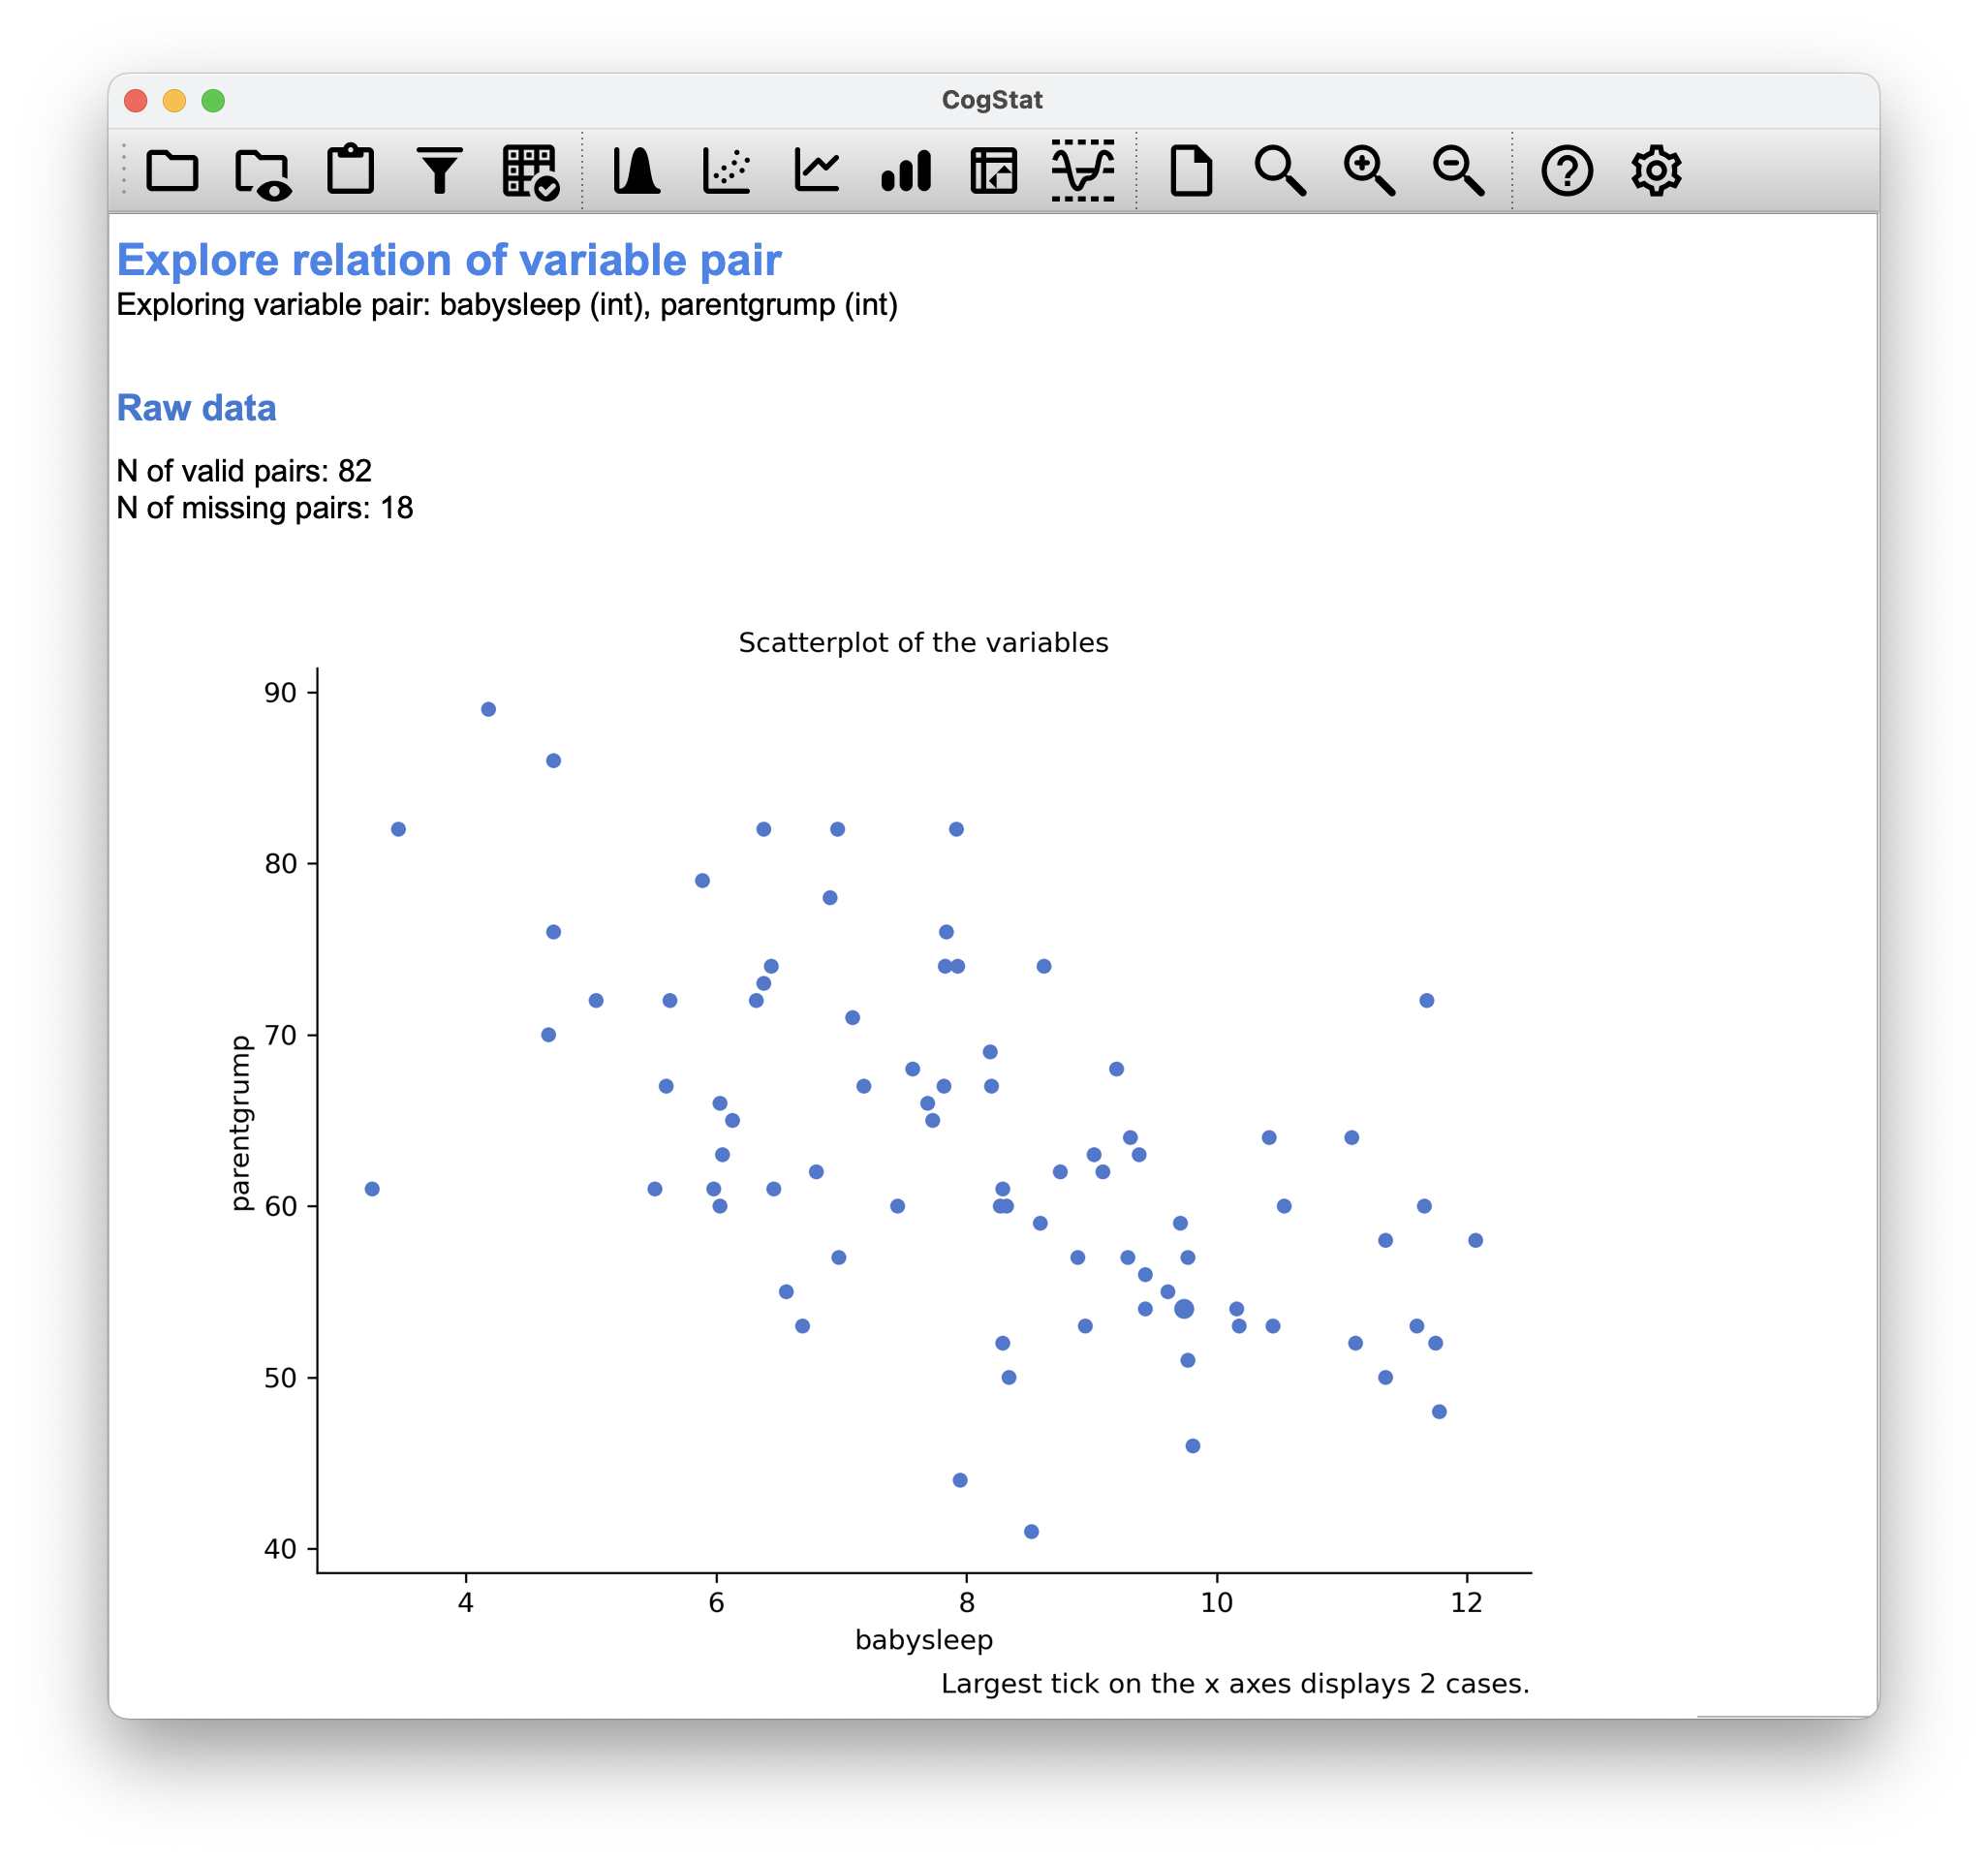
\includegraphics[width=0.66\linewidth]{resources/image/cogstatbabysleepparentgrumpmissing} 

}

\caption{18 missing pairs when comparing `babysleep` and `parentgrump`}\label{fig:parenthoodmissingcog2}
\end{figure}

\begin{figure}

{\centering 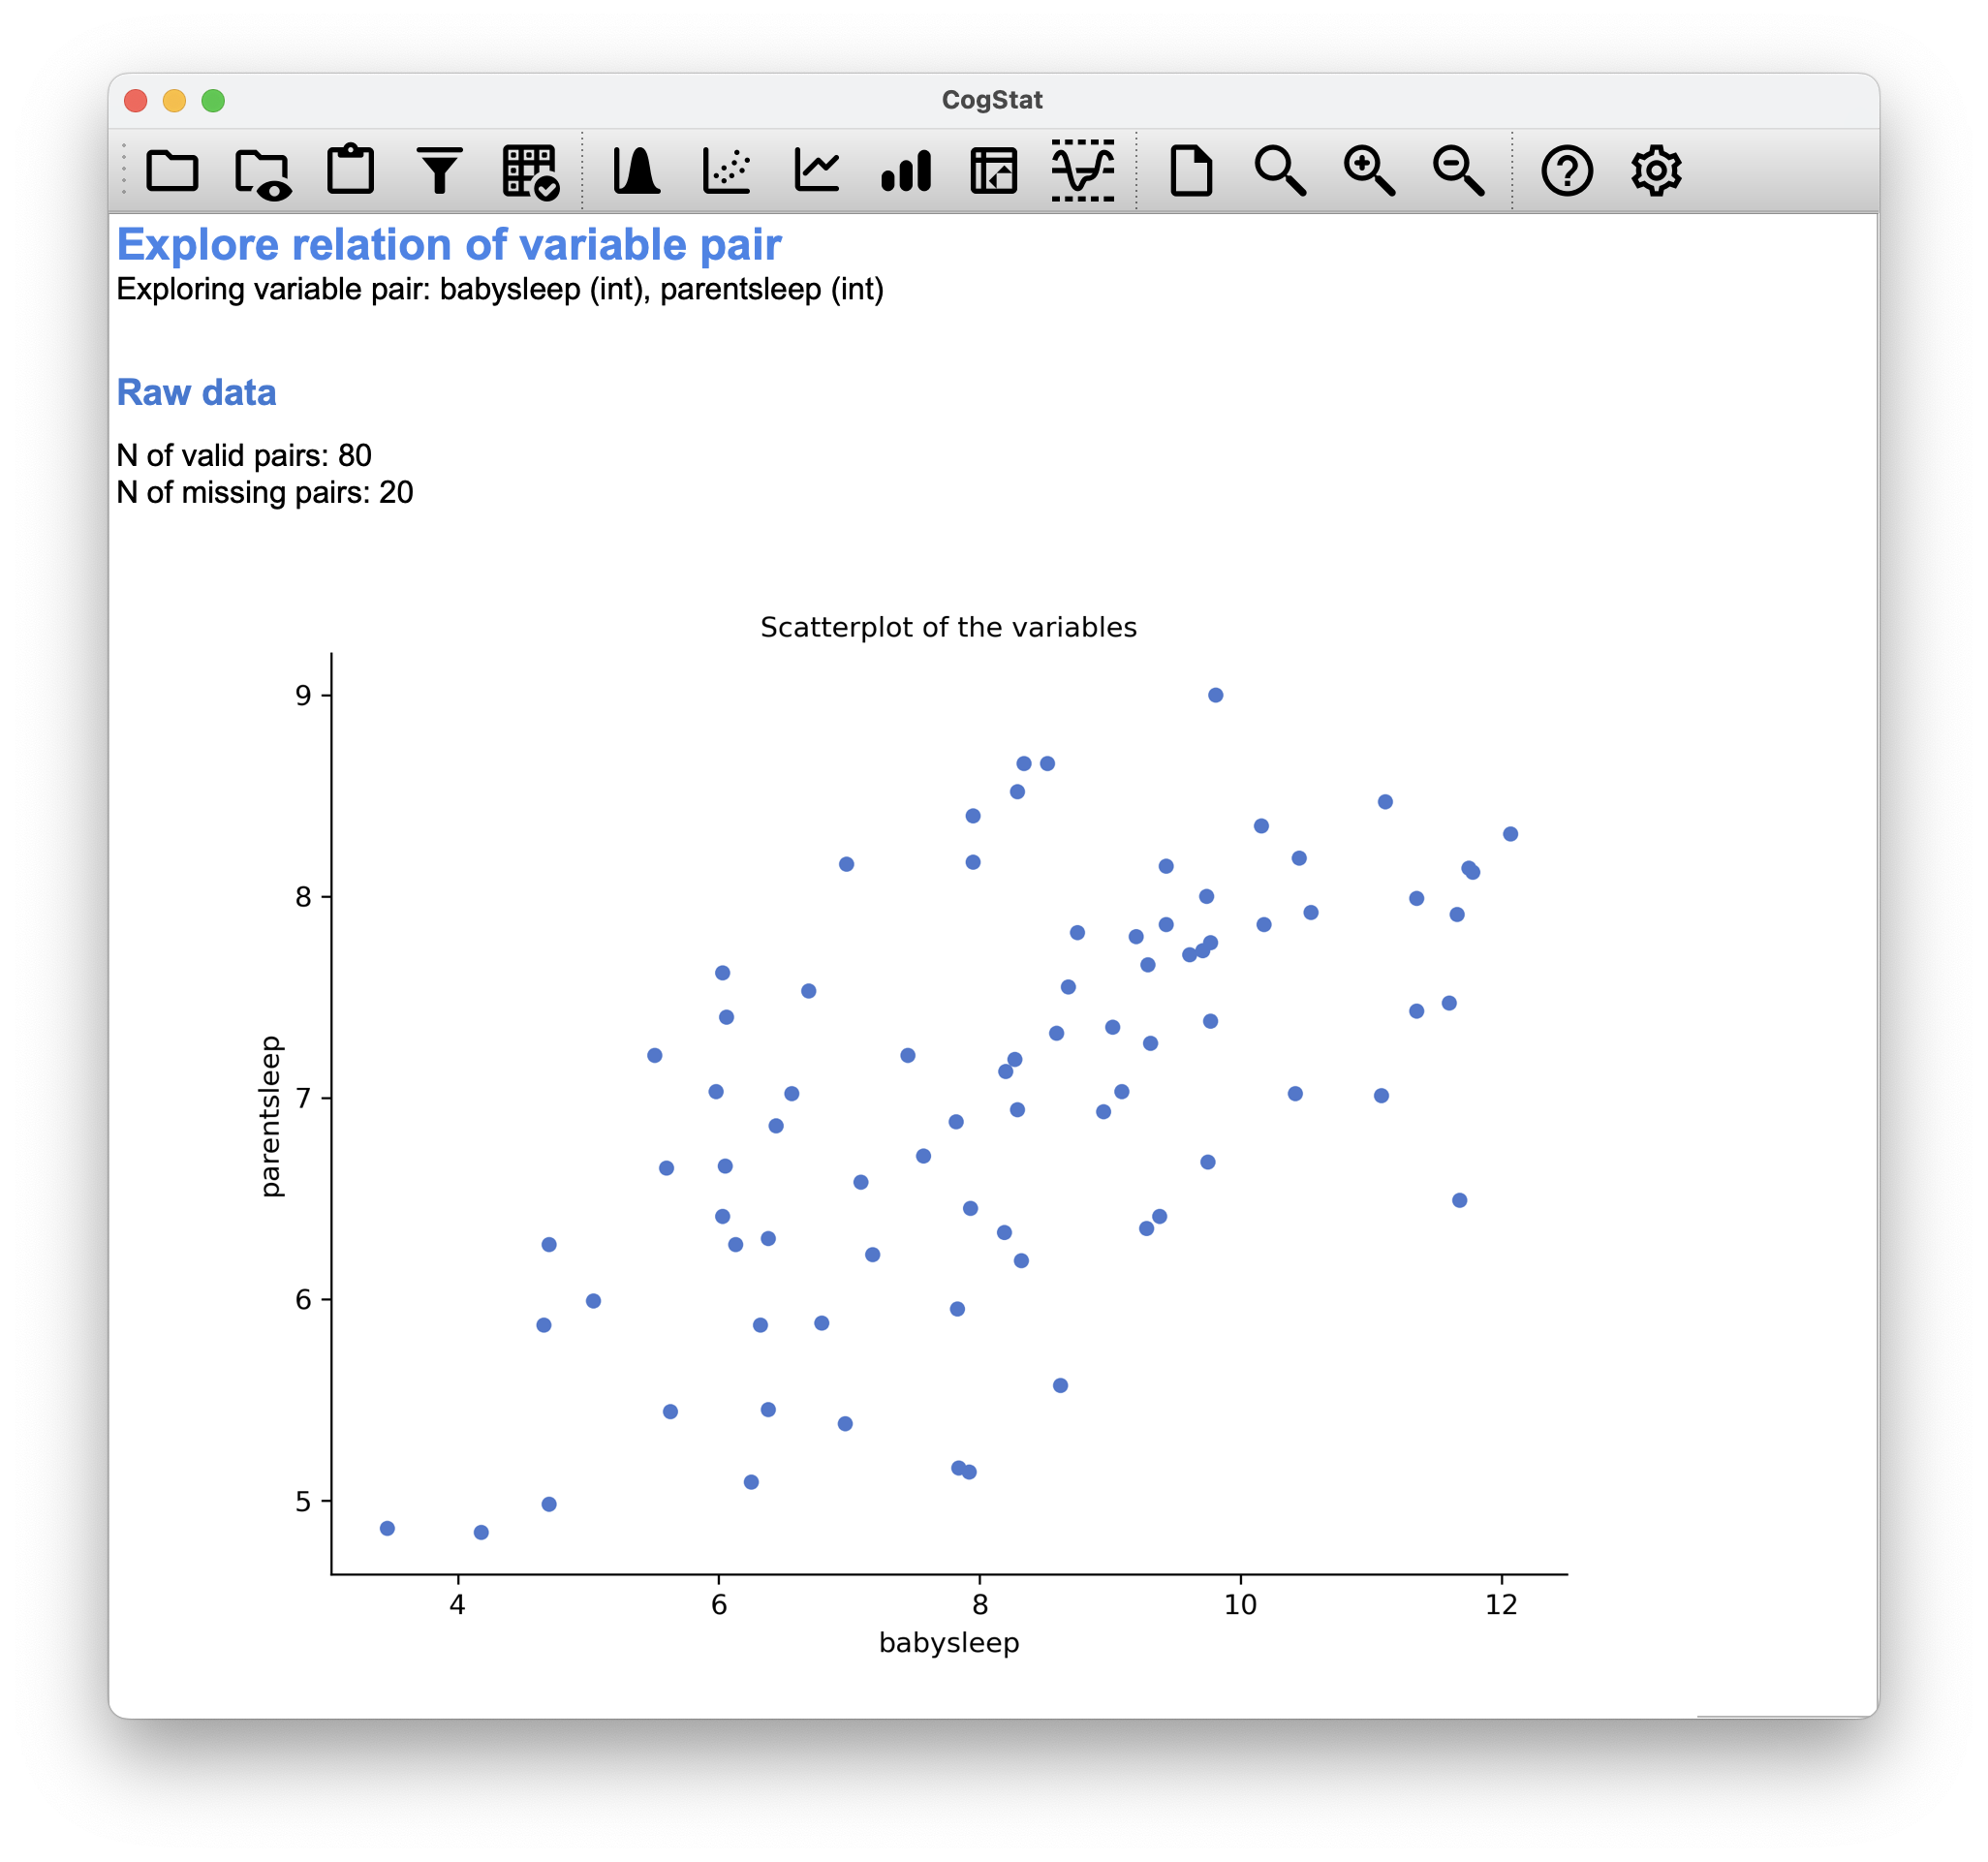
\includegraphics[width=0.66\linewidth]{resources/image/cogstatparentsleepbabysleepmissing} 

}

\caption{20 missing pairs when comparing `babysleep` and `parentsleep`}\label{fig:parenthoodmissingcog3}
\end{figure}

\hypertarget{summary-1}{%
\section{Summary}\label{summary-1}}

In this chapter, we discussed how to measure the strength of the relationship between two variables. We introduced the concept of correlation and how to calculate it using CogStat. We also discussed the difference between \textbf{Pearson's correlation} (Chapter \ref{pearson}) and \textbf{Spearman's rank order correlation} (Chapter \ref{spearman}), and how CogStat will calculate it for you. Finally, we discussed how CogStat handles missing values (Chapter \ref{missingvaluespair}) in pairwise calculations.

You might have been tempted to look at the regression coefficient, the linear regression formula etc. when exploring the results from CogStat. Don't worry, you'll have a chance to learn about these in Chapter \ref{regression}.

\hypertarget{part-inferential-statistics}{%
\part*{INFERENTIAL STATISTICS}\label{part-inferential-statistics}}
\addcontentsline{toc}{part}{INFERENTIAL STATISTICS}

\hypertarget{probability}{%
\chapter{Probability and distributions}\label{probability}}

A valuable part of statistics provides tools that let you make \emph{inferences} about data. Once you start thinking about statistics in these terms -- that statistics are there to help us draw inferences from data -- you start seeing examples everywhere. For instance, here's a small extract from a newspaper article in the Sydney Morning Herald (30 Oct 2010):

\begin{quote}
``I have a tough job,'' the Premier said in response to a poll which found her government is now the most unpopular Labor administration in polling history, with a primary vote of just 23 per cent.
\end{quote}

This kind of remark is unremarkable in the papers or in everyday life, but let's consider what it entails. A polling company has conducted an extensive survey because they can afford it. Let's imagine that they called 1000 NSW voters at random, and 230 (23\%) of those claimed that they intended to vote for the ALP. For the 2010 Federal election, the Australian Electoral Commission reported 4,610,795 enrolled voters in NSW, so the opinions of the remaining 4,609,795 voters (about 99.98\% of voters) remain unknown to us. Even assuming that no one lied to the polling company, we can only say with 100\% confidence that the actual ALP primary vote is somewhere between 230/4610795 (about 0.005\%) and 4610025/4610795 (about 99.83\%). So, on what basis is it legitimate for the polling company, the newspaper, and the readership to conclude that the ALP primary vote is only about 23\%?

The answer to the question is pretty obvious: if we call 1000 people at random, and 230 of them say they intend to vote for the ALP, then it seems very unlikely that these are the \emph{only} 230 people out of the entire voting public who actually intend to do so. In other words, we assume that the data collected by the polling company is pretty representative of the population at large. But how representative? Would we be surprised to discover that the true ALP primary vote is actually 24\%? 29\%? 37\%? At this point, everyday intuition starts to break down a bit. No one would be surprised by 24\%, and everybody would be surprised by 37\%, but it's hard to say whether 29\% is plausible. We need more powerful tools than just looking at the numbers and guessing.

\textbf{Inferential statistics} provides the tools we need to answer these questions. Since these questions lie at the heart of the scientific enterprise, they take up the lion's share of every introductory course on statistics and research methods. However, the theory of statistical inference is built on top of \textbf{probability theory}. And it is to probability theory that we must now turn. This discussion of probability theory is basically background: there's not a lot of statistics per se in this chapter, and you don't need to understand this material in as much depth as in the other chapters in this part of the book. Nevertheless, because probability theory does underpin so much of statistics, it's worth covering some of the basics.

\hypertarget{probabilitystats}{%
\section{How are probability and statistics different?}\label{probabilitystats}}

Before discussing probability theory, it's helpful to consider the relationship between probability and statistics. The two disciplines are closely related, but they're not identical. Probability theory is ``the doctrine of chances''. It's a branch of mathematics that tells you how often different events will happen. For example, all of these questions are things you can answer using probability theory:

\begin{itemize}
\tightlist
\item
  What are the chances of a fair coin coming up heads 10 times in a row?
\item
  If we roll two six-sided dice, how likely is it that we'll roll two sixes?
\item
  How likely is it that five cards drawn from a perfectly shuffled deck will all be hearts?
\item
  What are the chances that we'll win the lottery?
\end{itemize}

Notice that all of these questions have something in common. In each case the ``truth of the world'' is known, and my question relates to the ``what kind of events'' will happen. In the first question, we \emph{know} that the coin is fair, so there's a 50\% chance that any individual coin flip will come up heads. In the second question, we \emph{know} that the chance of rolling a 6 on a single die is 1 in 6. In the third question, we \emph{know} that the deck is shuffled properly. And in the fourth question, we \emph{know} that the lottery follows specific rules. You get the idea. The critical point is that probabilistic questions start with a known \textbf{\emph{model}} of the world, and we use that model to do some calculations. The underlying model can be quite simple. For instance, in the coin flipping example, we can write down the model like this:
\[
P(\mbox{heads}) = 0.5
\]
which you can read as ``the probability of heads is 0.5''. As we'll see later, in the same way, percentages are numbers that range from 0\% to 100\%, and probabilities are just numbers that range from 0 to 1. When using this probability model to answer the first question, we don't know exactly what will happen. Maybe we'll get 10 heads like the question says. But perhaps we'll get three heads. That's the key thing: in probability theory, the \emph{model} is known, but the \emph{data} are not.

So that's probability. What about statistics? Statistical questions work the other way around. In statistics, we \emph{do not} know the truth about the world. All we have is the data from which we want to \emph{learn} the truth about the world. Statistical questions tend to look more like these:

\begin{itemize}
\tightlist
\item
  If a friend flips a coin 10 times and gets 10 heads, are they playing a trick?
\item
  If five cards off the top of the deck are all hearts, how likely is it that the deck was shuffled?
\item
  If the lottery commissioner's spouse wins the lottery, how likely is it that the lottery was rigged?
\end{itemize}

This time around, the only thing we have are data. What we \emph{know} is that we saw a friend flip the coin 10 times, and it came up heads every time. And what we want to \textbf{infer} is whether or not we should conclude that what we just saw was actually a fair coin being flipped 10 times in a row, or whether we should suspect that the friend is playing a trick on us. The data we have look like this:

\begin{verbatim}
H H H H H H H H H H H
\end{verbatim}

and what we're trying to do is work out which ``model of the world'' we should put my trust in. If the coin is fair, then the model we should adopt is one that says that the probability of heads is 0.5; that is, \(P(\mbox{heads}) = 0.5\). If the coin is not fair, then we should conclude that the probability of heads is \emph{not} 0.5, which we would write as \(P(\mbox{heads}) \neq 0.5\). In other words, the statistical inference problem is to figure out which of these probability models is right. Clearly, the statistical question isn't the same as the probability question, but they're deeply connected to one another. Because of this, a good introduction to statistical theory will start with a discussion of what probability is and how it works.

\hypertarget{probabilitymeaning}{%
\section{What does probability mean?}\label{probabilitymeaning}}

Let's start with the first of these questions. What is ``probability''? It might seem surprising to you, but while statisticians and mathematicians (mostly) agree on what the \emph{rules} of probability are, there's much less of a consensus on what the word really \emph{means}. It seems weird because we're all very comfortable using words like ``chance'', ``likely'', ``possible'', and ``probable'', and it doesn't seem like it should be a complicated question to answer. If you had to explain ``probability'' to a five-year-old, you could do a pretty good job. But if you've ever had that experience in real life, you might walk away from the conversation feeling like you didn't quite get it right and that (like many everyday concepts) it turns out that you don't \emph{really} know what it's all about.

Let's suppose we want to bet on a soccer game between two teams of robots, \emph{Arduino Arsenal} and \emph{C Milan}. After thinking about it, we decide that there is an 80\% probability that \emph{Arduino Arsenal} winning. What do we mean by that? Here are three possibilities:

\begin{itemize}
\tightlist
\item
  They're robot teams, so we can make them play over and over again, and if we did that, \emph{Arduino Arsenal} would win 8 out of every 10 games on average.
\item
  For any given game, we would only agree that betting on this game is only ``fair'' if a \$1 bet on \emph{C Milan} gives a \$5 payoff (i.e.~we get \$1 back plus a \$4 reward for being correct), as would a \$4 bet on \emph{Arduino Arsenal} (i.e., \$4 bet plus a \$1 reward).
\item
  Our subjective ``belief'' or ``confidence'' in an \emph{Arduino Arsenal} victory is four times as strong as our belief in a \emph{C Milan} victory.
\end{itemize}

Each of these seems sensible. However, they're not identical, and not every statistician would endorse all of them. The reason is that there are different statistical ideologies (yes, really!) and depending on which one you subscribe to, you might say that some of those statements are meaningless or irrelevant. In this section, we give a brief introduction to the two main approaches that exist in the literature. These are by no means the only approaches, but they're the two big ones.

\hypertarget{the-frequentist-view}{%
\subsection{The frequentist view}\label{the-frequentist-view}}

The first of the two major approaches to probability, and the more dominant one in statistics, is referred to as the \textbf{\emph{frequentist view}}, which defines probability as a \textbf{\emph{long-run frequency}}. Suppose we were to try flipping a fair coin over and over again. By definition, this is a coin that has \(P(H) = 0.5\). What might we observe? One possibility is that the first 20 flips might look like this:

\begin{verbatim}
T,H,H,H,H,T,T,H,H,H,H,T,H,H,T,T,T,T,T,H
\end{verbatim}

In this case, 11 of these 20 coin flips (55\%) came up heads. Now suppose that we'd been keeping a running tally of the number of heads (which we'll call \(N_H\)) that we've seen, across the first \(N\) flips, and calculate the proportion of heads \(N_H / N\) every time. Here's what we'd get:

\begin{longtable}[]{@{}ccc@{}}
\toprule()
Number of flips & Number of heads & Proportion of heads \\
\midrule()
\endhead
1 & 0 & 0.00 \\
2 & 1 & 0.50 \\
3 & 2 & 0.67 \\
4 & 3 & 0.75 \\
5 & 4 & 0.80 \\
6 & 4 & 0.67 \\
7 & 4 & 0.57 \\
8 & 5 & 0.63 \\
9 & 6 & 0.67 \\
10 & 7 & 0.70 \\
11 & 8 & 0.73 \\
12 & 8 & 0.67 \\
13 & 9 & 0.69 \\
14 & 10 & 0.71 \\
15 & 10 & 0.67 \\
16 & 10 & 0.63 \\
17 & 10 & 0.59 \\
18 & 10 & 0.56 \\
19 & 10 & 0.53 \\
20 & 11 & 0.55 \\
\bottomrule()
\end{longtable}

Notice that at the start of the sequence, the \emph{proportion} of heads fluctuates wildly, starting at .00 and rising as high as .80. Later on, one gets the impression that it dampens out a bit, with more and more of the values actually being pretty close to the ``right'' answer of .50. This is the frequentist definition of probability in a nutshell: flip a fair coin over and over again, and as \(N\) grows large (approaches infinity, denoted \(N\rightarrow \infty\)), the proportion of heads will converge to 50\%. There are some subtle technicalities that mathematicians care about, but qualitatively speaking, that's how the frequentists define probability. Unfortunately, we don't have an infinite number of coins, or the infinite patience required to flip a coin an infinite number of times. However, we do have a computer, and computers excel at mindless repetitive tasks. So let's ask a computer to simulate flipping a coin 1000 times, and then draw a picture of what happens to the proportion \(N_H / N\) as \(N\) increases. The results are shown in Figure \ref{fig:frequentistprobability}. As you can see, the \emph{proportion of observed heads} eventually stops fluctuating, and settles down; when it does, the number at which it finally settles is the true probability of heads.

\begin{figure}

{\centering 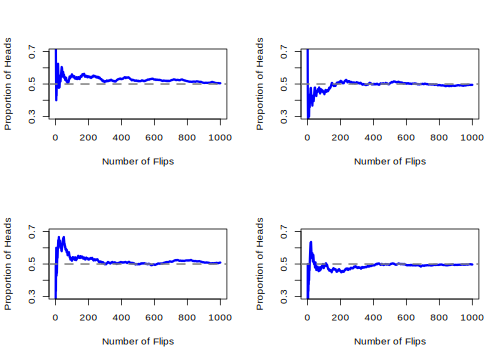
\includegraphics[width=0.66\linewidth]{lsc_files/figure-latex/frequentistprobability-1} 

}

\caption{An illustration of how frequentist probability works. If you flip a fair coin over and over again, the proportion of heads that you've seen eventually settles down, and converges to the true probability of 0.5. Each panel shows four different simulated experiments: in each case, we pretend we flipped a coin 1000 times, and kept track of the proportion of flips that were heads as we went along. Although none of these sequences actually ended up with an exact value of .5, if we'd extended the experiment for an infinite number of coin flips they would have.}\label{fig:frequentistprobability}
\end{figure}

The frequentist definition of probability has some desirable characteristics. Firstly, it is objective: the probability of an event is \emph{necessarily} grounded in the world. The only way that probability statements can make sense is if they refer to (a sequence of) events that occur in the physical universe.\footnote{This doesn't mean that frequentists can't make hypothetical statements, of course; it's just that if you want to make a statement about probability, then it must be possible to redescribe that statement in terms of a sequence of potentially observable events, and the relative frequencies of different outcomes that appear within that sequence.} Secondly, it is unambiguous: any two people watching the same sequence of events unfold, trying to calculate the probability of an event, must inevitably come up with the same answer. However, it also has undesirable characteristics. Firstly, infinite sequences don't exist in the physical world. Suppose you picked up a coin from your pocket and started to flip it. Every time it lands, it impacts the ground. Each impact wears the coin down a bit; eventually, the coin will be destroyed. So, one might ask whether it really makes sense to pretend that an ``infinite'' sequence of coin flips is even a meaningful concept or an objective one. We can't say that an ``infinite sequence'' of events is a real thing in the physical universe because the physical universe doesn't allow infinite anything. More seriously, the frequentist definition has a narrow scope. There are many things out there that human beings are happy to assign a probability to in everyday language but cannot (even in theory) be mapped onto a hypothetical sequence of events. For instance, if a meteorologist comes on TV and says, ``the probability of rain in Adelaide on 2 November 2048 is 60\%'', we humans are happy to accept this. But it's not clear how to define this in frequentist terms. There's only one city of Adelaide, and only 2 November 2048. There's no infinite sequence of events here, just a once-off thing. Frequentist probability genuinely \emph{forbids} us from making probability statements about a single event. From the frequentist perspective, it will either rain tomorrow or not; there is no ``probability'' that attaches to a single non-repeatable event. Now, it should be said that there are some very clever tricks that frequentists can use to get around this. One possibility is that what the meteorologist means is something like this: ``There is a category of days for which we predict a 60\% chance of rain; if we look only across those days for which we make this prediction, then on 60\% of those days it will actually rain''. It's very weird and counterintuitive to think of it this way, but you do see frequentists do this sometimes. And it \emph{will} come up later in this book (see Chapter \ref{ci}).

\hypertarget{the-bayesian-view}{%
\subsection{The Bayesian view}\label{the-bayesian-view}}

The \textbf{Bayesian view} of probability is often called the \emph{subjectivist view}, and it is a minority view among statisticians but one that has been steadily gaining traction for the last several decades. There are many flavours of Bayesianism, making it hard to say what ``the'' Bayesian view is. The most common way of thinking about subjective probability is to define the probability of an event as the \textbf{degree of belief} that an intelligent and rational agent assigns to the truth of that event. From that perspective, probabilities don't exist in the world but rather in the thoughts and assumptions of people and other intelligent beings.
However, for this approach to work, we need some way of operationalising the ``degree of belief''. One way you can do this is to formalise it in terms of ``rational gambling'', though there are many other ways. Suppose that we believe that there's a 60\% probability of rain tomorrow. If someone offers us a bet: if it rains tomorrow, then we win \$5, but if it doesn't rain, then we lose \$5. Clearly, from our perspective, this is a pretty good bet. On the other hand, if we think the probability of rain is only 40\%, then it's a bad bet. Thus, we can operationalise the notion of a ``subjective probability'' in terms of what bets we're willing to accept.

What are the advantages and disadvantages of the Bayesian approach? The main advantage is that it allows you to assign probabilities to any event you want to. You don't need to be limited to those events that are repeatable. The main disadvantage (to many people) is that we can't be purely objective -- specifying a probability requires us to specify an entity with the relevant degree of belief. This entity might be a human, an alien, a robot, or even a statistician, but there has to be an intelligent agent out there that believes in things. To many people, this is uncomfortable: it seems to make probability arbitrary. While the Bayesian approach does require that the agent in question be rational (i.e., obey the rules of probability), it does allow everyone to have their own beliefs; I can believe the coin is fair, and you don't have to, even though we're both rational. The frequentist view doesn't allow any two observers to attribute different probabilities to the same event: when that happens, then at least one of them must be wrong. The Bayesian view does not prevent this from occurring. Two observers with different background knowledge can legitimately hold different beliefs about the same event. In short, where the frequentist view is sometimes considered to be too narrow (forbids lots of things that that we want to assign probabilities to), the Bayesian view is sometimes thought to be too broad (allows too many differences between observers).

\hypertarget{whats-the-difference-and-who-is-right}{%
\subsection{What's the difference? And who is right?}\label{whats-the-difference-and-who-is-right}}

Now that you've seen these two views independently, it's useful to make sure you can compare them. Go back to the hypothetical robot soccer game at the start of the section. What would a frequentist and a Bayesian say about these three statements? Which statement would a frequentist say is the correct definition of probability? Which one would a Bayesian do? Would some of these statements be meaningless to a frequentist or a Bayesian? If you've understood the two perspectives, you should have some sense of how to answer those questions.

Okay, assuming you understand the difference, you might be wondering which of them is \emph{right}? Honestly, we don't know that there is a right answer. As far as we can tell, there's nothing mathematically incorrect about the way frequentists think about sequences of events, and there's nothing mathematically incorrect about the way that Bayesians define the beliefs of a rational agent. In fact, when you dig down into the details, Bayesians and frequentists actually agree about a lot of things. Many frequentist methods lead to decisions that Bayesians agree a rational agent would make. Many Bayesian methods have very good frequentist properties.

Consider Sir Ronald Fisher, one of the towering figures of 20th-century statistics and a vehement opponent of all things Bayesian, whose paper on the mathematical foundations of statistics referred to Bayesian probability as ``an impenetrable jungle {[}that{]} arrests progress towards precision of statistical concepts'' Fisher (\protect\hyperlink{ref-Fisher1922b}{1922b}). Or the psychologist Paul Meehl, who suggests that relying on frequentist methods could turn you into ``a potent but sterile intellectual rake who leaves in his merry path a long train of ravished maidens but no viable scientific offspring'' Meehl (\protect\hyperlink{ref-Meehl1967}{1967}). The history of statistics, as you might gather, is not devoid of entertainment.

In any case, while Danielle personally prefers the Bayesian view, the majority of statistical analyses are based on the frequentist approach. My reasoning is pragmatic: the goal of this book is to cover roughly the same territory as a typical undergraduate stats class in psychology, and if you want to understand the statistical tools used by most psychologists, you'll need a good grasp of frequentist methods. We promise you that this isn't a wasted effort. Even if you end up wanting to switch to the Bayesian perspective, you really should read through at least one book on the ``orthodox'' frequentist view. Every now and then, we'll add some commentary from a Bayesian point of view, and we'll revisit the topic in more depth in Chapter \ref{bayes}.

\hypertarget{basicprobability}{%
\section{Basic probability theory}\label{basicprobability}}

Although there are ideological arguments between Bayesians and frequentists, it turns out that people mostly agree on the rules that probabilities should obey. There are lots of different ways of arriving at these rules. The most commonly used approach is based on the work of Andrey Kolmogorov, one of the great Soviet mathematicians of the 20th century. Without going into a lot of detail, we'll try to give you a sense of how it works.

Let's assume we own five pairs of pants: three pairs of jeans, the bottom half of a suit, and a pair of tracksuit pants. Let's call them \(X_1\), \(X_2\), \(X_3\), \(X_4\) and \(X_5\). Now, on any given day, we pick out exactly one pair of pants. If we were to describe this situation using the language of probability theory, we would refer to each pair of pants (i.e., each \(X\)) as an \textbf{elementary event}. The key characteristic of elementary events is that every time we make an observation (e.g., every time we put on a pair of pants), then the outcome will be one and only one of these events. As said, we only wear exactly one pair of pants, so it satisfies this constraint. Similarly, the set of all possible events is called a \textbf{sample space}.

Okay, now that we have a sample space (a wardrobe) built from lots of possible elementary events (pants), we want to assign a \textbf{probability} of one of these elementary events. For an event \(X\), the probability of that event \(P(X)\) is a number that lies between 0 and 1. The bigger the value of \(P(X)\), the more likely the event will occur. So, for example, if \(P(X) = 0\), it means the event \(X\) is impossible (i.e., we never wear those pants). On the other hand, if \(P(X) = 1\) it means that event \(X\) is certain to occur (i.e., we always wear those pants). For probability values in the middle, it means that we sometimes wear those pants. For instance, if \(P(X) = 0.5\), it means that we wear those pants half of the time.

At this point, we're almost done. The last thing we need to recognise is that ``something always happens''. Every time we put on pants, we really do end up wearing pants (crazy, right?). What this somewhat trite statement means, in probabilistic terms, is that the probabilities of the elementary events need to add up to 1. This is known as the \textbf{law of total probability}. More importantly, if these requirements are satisfied, then we have a \textbf{probability distribution}. For example, this is an example of a probability distribution:

\begin{table}
\centering
\begin{tabular}{llllll}
\toprule
 & Blue jeans & Grey jeans & Black jeans & Black suit & Blue tracksuit\\
\midrule
Label & $X_1$ & $X_2$ & $X_3$ & $X_4$ & $X_5$\\
Probability & $P(X_1) = .5$ & $P(X_2) = .3$ & $P(X_3) = .1$ & $P(X_4) = 0$ & $P(X_5) = .1$\\
\bottomrule
\end{tabular}
\end{table}

Each of the events has a probability that lies between 0 and 1, and if we add up the probability of all events, they sum to 1, as shown in Figure \ref{fig:pantsprob}. And at this point, we've all achieved something. You've learned what probability distribution is.

\begin{figure}

{\centering 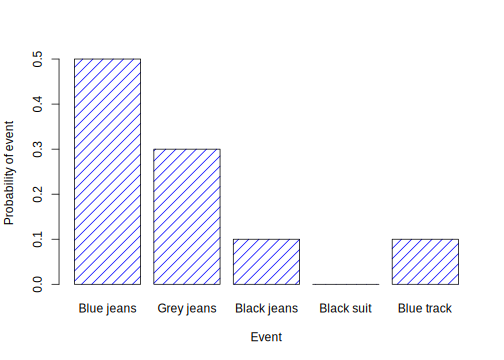
\includegraphics[width=0.66\linewidth]{lsc_files/figure-latex/pantsprob-1} 

}

\caption{A visual depiction of the "pants" probability distribution. There are five "elementary events", corresponding to the five pairs of pants. Each event has some probability of occurring: this probability is a number between 0 to 1. The sum of these probabilities is 1.}\label{fig:pantsprob}
\end{figure}

The only other thing that needs pointing out is that probability theory allows you to talk about \textbf{non-elementary events} as well as elementary ones. The easiest way to illustrate the concept is with an example. In the pants example, it's legitimate to refer to the probability that we wear jeans. In this scenario, the ``We wear jeans'' event is said to have happened as long as the elementary event that actually did occur is one of the appropriate ones; in this case ``blue jeans'', ``black jeans'', or ``grey jeans''. In mathematical terms, we defined the ``jeans'' event \(E\) to correspond to the set of elementary events \((X_1, X_2, X_3)\). If any of these elementary events occurs, then \(E\) is also said to have occurred. Having decided to write down the definition of the \(E\) this way, it's pretty straightforward to state what the probability \(P(E)\) is: we just add everything up. In this particular case
\[
P(E) = P(X_1) + P(X_2) + P(X_3)
\]
and, since the probabilities of blue, grey and black jeans respectively are .5, .3 and .1, the probability that we wear jeans is equal to .9.

At this point, you might be thinking that this is all terribly obvious and simple, and you'd be right. All we've done is wrap some basic mathematics around a few common sense intuitions. However, from these simple beginnings, it's possible to construct some extremely powerful mathematical tools. Without going into the details in this book, we list -- in Table \ref{tab:probrules} -- some of the other rules that probabilities satisfy. These rules can be derived from the simple assumptions that we've outlined above.

\begin{table}[!h]

\caption{\label{tab:probrules}Some basic rules that probabilities must satisfy. You don't really need to know these rules in order to understand the analyses that we'll talk about later in the book, but they are important if you want to understand probability theory a bit more deeply.}
\centering
\begin{tabular}[t]{llll}
\toprule
English & Notation &  & Formula\\
\midrule
Not $A$ & $P(\neg A)$ & = & $1-P(A)$\\
$A$ or $B$ & $P(A \cup B)$ & = & $P(A) + P(B) - P(A \cap B)$\\
$A$ and $B$ & $P(A \cap B)$ & = & $P(A|B) P(B)$\\
\bottomrule
\end{tabular}
\end{table}

\hypertarget{distributions}{%
\section{Distributions}\label{distributions}}

As you might imagine, probability distributions vary enormously, and there's an enormous range of distributions. However, they aren't all equally important. In fact, the vast majority of the content in this book relies on one of five distributions: the binomial distribution, the normal distribution, the \(t\) distribution, the \(\chi^2\) (``chi-square'') distribution and the \(F\) distribution. Given this, the next few sections will briefly introduce all five of these, paying special attention to the binomial and the normal.

\hypertarget{binomial}{%
\subsection{The binomial distribution}\label{binomial}}

The theory of probability originated in an attempt to describe how games of chance work. Hence, it seems fitting that our discussion of the \textbf{binomial distribution} should involve a discussion of rolling dice and flipping coins. Let's imagine a simple ``experiment'': we're holding 20 identical six-sided dice. There's a picture of a skull on one face of each die; the other five faces are all blank. If we roll all 20 dice, what's the probability of getting exactly 4 skulls? Assuming that the dice are fair, we know that the chance of any one die coming up skulls is 1 in 6; to say this another way, the skull probability for a single die is approximately \(0.167\). This is enough information to answer our question, so let's have a look at how it's done.

As usual, we'll want to introduce some names and some notation. We'll let \(N\) denote the number of dice rolls in our experiment, which is often referred to as the \textbf{size parameter} of our binomial distribution. We'll also use \(\theta\) to refer to the probability that a single die comes up skulls, a quantity that is usually called the \textbf{success probability} of the binomial.\footnote{Note that the term ``success'' is pretty arbitrary and doesn't actually imply that the outcome is something to be desired. If \(\theta\) referred to the probability that any one passenger gets injured in a bus crash, it is still called the success probability.} Finally, we'll use \(X\) to refer to the results of our experiment, namely the number of skulls we get when rolling the dice. Since the actual value of \(X\) is due to chance, we refer to it as a \textbf{random variable}. In any case, now that we have all this terminology and notation, we can use it to state the problem a little more precisely. The quantity that we want to calculate is the probability that \(X = 4\) given that we know that \(\theta = .167\) and \(N=20\). The general ``form'' of the thing could be written as
\[
P(X \ | \ \theta, N)
\]
and we're interested in the special case where \(X=4\), \(\theta = 0.167\) and \(N=20\).
There's only one more piece of notation. If we want to say that \(X\) is generated randomly from a binomial distribution with parameters \(\theta\) and \(N\), the notation is as follows:
\[
X \sim \mbox{Binomial}(\theta, N)
\]

Yeah, yeah. I know what you're thinking: notation, notation, notation. Really, who cares? Very few readers of this book are here for the notation, so we should probably move on and talk about how to use the binomial distribution. We've included the formula for the binomial distribution in Table \ref{tab:distformulas}, since some readers may want to play with it themselves, but since most people probably don't care that much and because we don't need the formula in this book, let's not talk about it in any detail. Instead, let's just see what the binomial distribution looks like. To that end, Figure \ref{fig:binomial1} plots the binomial probabilities for all possible values of \(X\) for our dice rolling experiment, from \(X=0\) (no skulls) all the way up to \(X=20\) (all skulls). Note that this is basically a bar chart, and is no different to the ``pants probability'' plot in Figure \ref{fig:pantsprob}. On the horizontal axis we have all the possible events, and on the vertical axis we can read off the probability of each of those events. So, the probability of rolling 4 skulls out of 20 times is about 0.20 (the actual answer is 0.2022036). In other words, you'd expect that to happen about 20\% of the times you repeated this experiment.

\begin{table}

\caption{\label{tab:distformulas}Formulas for the binomial and normal distributions. We don't use these formulas for anything in this book, but they're pretty important for more advanced work. In the equation for the binomial, $X!$ is the factorial function (i.e., multiply all whole numbers from 1 to $X$), and for the normal distribution "exp" refers to the exponential function, which we discussed in the Chapter on Data Handling. If these equations don't make a lot of sense to you, don't worry too much about them.}
\centering
\begin{tabular}[t]{ll}
\toprule
Binomial & Normal\\
\midrule
$P(X | \theta, N) = \displaystyle\frac{N!}{X! (N-X)!} \theta^X (1-\theta)^{N-X}$ & $p(X | \mu, \sigma) = \displaystyle\frac{1}{\sqrt{2\pi}\sigma} \exp \left( -\frac{(X - \mu)^2}{2\sigma^2} \right)$\\
\bottomrule
\end{tabular}
\end{table}

\begin{figure}

{\centering 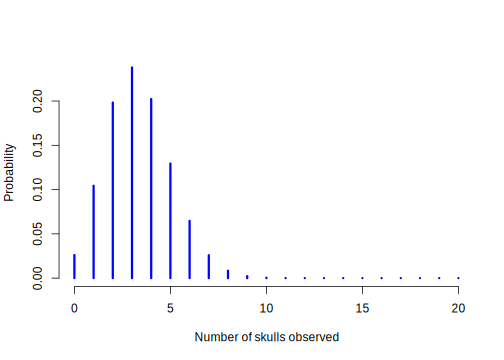
\includegraphics[width=0.66\linewidth]{lsc_files/figure-latex/binomial1-1} 

}

\caption{The binomial distribution with size parameter of $N=20$ and an underlying success probability of $theta = 1/6$. Each vertical bar depicts the probability of one specific outcome (i.e., one possible value of $X$). Because this is a probability distribution, each of the probabilities must be a number between 0 and 1, and the heights of the bars must sum to 1 as well.}\label{fig:binomial1}
\end{figure}

\hypertarget{normal}{%
\subsection{The normal distribution}\label{normal}}

While the binomial distribution is conceptually the simplest distribution to understand, it's not the most important one. That particular honour goes to the \textbf{normal distribution}, which is also referred to as ``the bell curve'' or ``Gaussian distribution''. A normal distribution is described using two parameters, the mean of the distribution \(\mu\) and the standard deviation of the distribution \(\sigma\). The notation that we sometimes use to say that a variable \(X\) is normally distributed is as follows:
\[
X \sim \mbox{Normal}(\mu,\sigma)
\]
Of course, that's just notation. It doesn't tell us anything relevant about the normal distribution itself. As was the case with the binomial distribution, the formula for the normal distribution in this book is tucked away in Table \ref{tab:distformulas}.

Instead of focusing on the maths, let's try to understand what it means for a variable to be normally distributed. To that end, have a look at Figure \ref{fig:normdist}, which plots a normal distribution with mean \(\mu = 0\) and standard deviation \(\sigma = 1\). You can see where the name ``bell curve'' comes from: it looks a bit like a bell. Notice that, unlike the plots to illustrate the binomial distribution, the picture of the normal distribution in Figure \ref{fig:normdist} shows a smooth curve instead of ``histogram-like'' bars. This isn't an arbitrary choice: the normal distribution is \emph{continuous}, whereas the binomial is \emph{discrete}. For instance, in the die rolling example from the last section, it was possible to get 3 skulls or 4 skulls, but impossible to get 3.9 skulls. The figures in the previous section reflected this fact: in Figure \ref{fig:binomial1}, for instance, there's a bar located at \(X=3\) and another one at \(X=4\), but there's nothing in between. Continuous quantities don't have this constraint. For instance, suppose we're talking about the weather. The temperature on a pleasant Spring day could be 23 degrees, 24 degrees, 23.9 degrees, or anything in between since temperature is a continuous variable, and so a normal distribution might be quite appropriate for describing Spring temperatures.\footnote{In practice, the normal distribution is so handy that people tend to use it even when the variable isn't actually continuous. As long as there are enough categories (e.g., Likert scale responses to a questionnaire), it's pretty standard practice to use the normal distribution as an approximation. This works out much better in practice than you'd think.}



\begin{figure}

{\centering 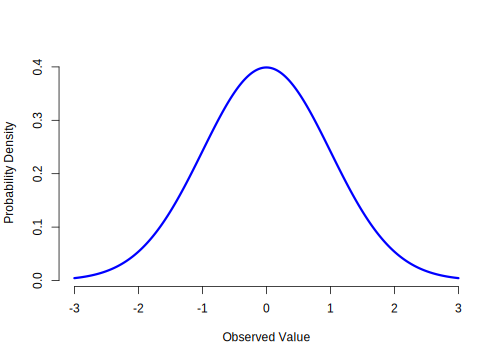
\includegraphics[width=0.66\linewidth]{lsc_files/figure-latex/normdist-1} 

}

\caption{The normal distribution with mean \(mu = 0\) and standard deviation \(sigma = 1\). The \(x\)-axis corresponds to the value of some variable, and the \(y\)-axis tells us something about how likely we are to observe that value. However, notice that the \(y\)-axis is labelled ``Probability Density'' and not ``Probability''. There is a subtle and somewhat frustrating characteristic of continuous distributions that makes the \(y\) axis behave a bit oddly: the height of the curve here isn't actually the probability of observing a particular \(x\) value. On the other hand, it \emph{is} true that the heights of the curve tells you which \(x\) values are more likely (the higher ones!).}\label{fig:normdist}
\end{figure}

With this in mind, let's see if we can get an intuition for how the normal distribution works. Firstly, let's have a look at what happens when we play around with the parameters of the distribution. To that end, Figure \ref{fig:normmean} plots normal distributions that have different means, but have the same standard deviation. As you might expect, all of these distributions have the same ``width''. The only difference between them is that they've been shifted to the left or to the right. In every other respect, they're identical.

In contrast, if we increase the standard deviation while keeping the mean constant, the peak of the distribution stays in the same place, but the distribution gets wider, as you can see in Figure \ref{fig:normsd}. Notice, though, that when we widen the distribution, the height of the peak shrinks. This has to happen: in the same way that the heights of the bars that we used to draw a discrete binomial distribution have to \emph{sum} to 1, the total \emph{area under the curve} for the normal distribution must equal 1.

\begin{figure}

{\centering 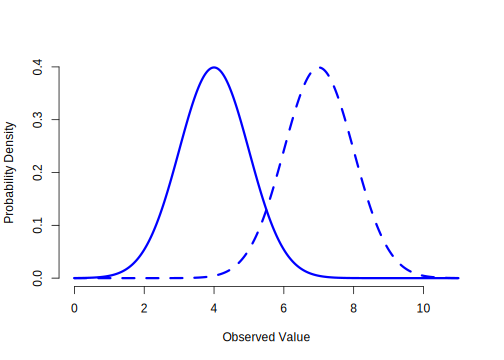
\includegraphics[width=0.66\linewidth]{lsc_files/figure-latex/normmean-1} 

}

\caption{An illustration of what happens when you change the mean of a normal distribution. The solid line depicts a normal distribution with a mean of $mu=4$. The dashed line shows a normal distribution with a mean of $mu=7$. In both cases, the standard deviation is $sigma=1$. Not surprisingly, the two distributions have the same shape, but the dashed line is shifted to the right.}\label{fig:normmean}
\end{figure}

\begin{figure}

{\centering 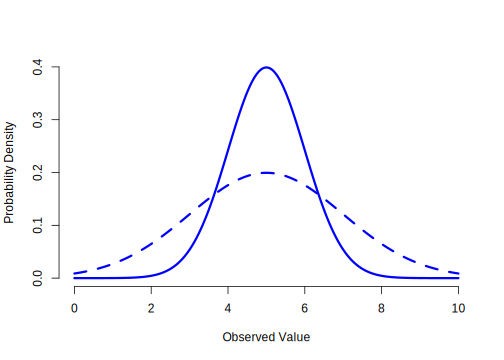
\includegraphics[width=0.66\linewidth]{lsc_files/figure-latex/normsd-1} 

}

\caption{An illustration of what happens when you change the the standard deviation of a normal distribution. Both distributions plotted in this figure have a mean of $mu = 5$, but they have different standard deviations. The solid line plots a distribution with standard deviation $sigma=1$, and the dashed line shows a distribution with standard deviation $sigma = 2$. As a consequence, both distributions are "centred" on the same spot, but the dashed line is wider than the solid one.}\label{fig:normsd}
\end{figure}

Before moving on, there is one important characteristic of the normal distribution to point out. Irrespective of the actual mean and standard deviation, 68.3\% of the area falls within 1 standard deviation of the mean. Similarly, 95.4\% of the distribution falls within 2 standard deviations of the mean, and 99.7\% of the distribution is within 3 standard deviations. This idea is illustrated in Figures \ref{fig:sdnorm1} and \ref{fig:sdnorm2}.

\textbackslash begin\{figure\}
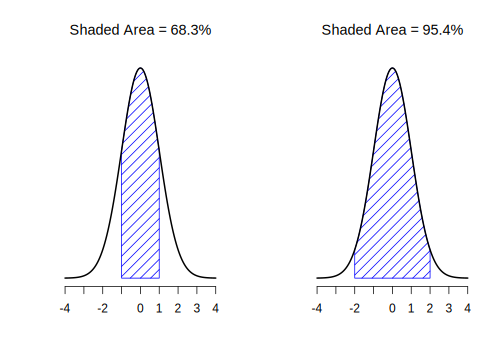
\includegraphics[width=0.66\linewidth]{lsc_files/figure-latex/sdnorm1-1} \textbackslash caption\{The area under the curve tells you the probability that an observation falls within a particular range. The solid lines plot normal distributions with mean \(mu=0\) and standard deviation \(sigma=1\). The shaded areas illustrate \emph{areas under the curve} for two important cases. On the left, we can see that there is a 68.3\% chance that an observation will fall within one standard deviation of the mean. On the right, we see that there is a 95.4\% chance that an observation will fall within two standard deviations of the mean\}\label{fig:sdnorm1}
\textbackslash end\{figure\}

\textbackslash begin\{figure\}
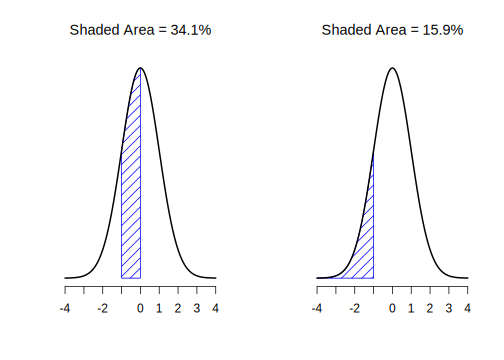
\includegraphics[width=0.66\linewidth]{lsc_files/figure-latex/sdnorm2-1} \textbackslash caption\{Two more examples of the \emph{area under the curve idea}. There is a 15.9\% chance that an observation is one standard deviation below the mean or smaller (left), and a 34.1\% chance that the observation is greater than one standard deviation below the mean but still below the mean (right). Notice that if you add these two numbers together you get 15.9\% + 34.1\% = 50\%. For normally distributed data, there is a 50\% chance that an observation falls below the mean. And of course that also implies that there is a 50\% chance that it falls above the mean.\}\label{fig:sdnorm2}
\textbackslash end\{figure\}

\hypertarget{density}{%
\subsection{Probability density}\label{density}}

There's something we missed throughout the discussion of the normal distribution, something that some introductory textbooks omit completely. Fortunately, it's not something that you need to understand at a deep level in order to do basic statistics: rather, it's something that starts to become important later on when you move beyond the basics. So, if it doesn't make complete sense, don't worry: try to make sure that you follow the gist of it.

There have been one or two things that don't quite make sense. Perhaps you noticed that the \(y\)-axis in these figures is labelled ``Probability Density'' rather than density. Maybe you noticed that we used \(p(X)\) instead of \(P(X)\) when giving the formula for the normal distribution.

Let us spend a little time thinking about what it really \emph{means} to say that \(X\) is a continuous variable. Let's say we're talking about the temperature outside. The thermometer tells me it's 23 degrees, but we know that's not really true. It's not \emph{exactly} 23 degrees. Maybe it's 23.1 degrees. But we know that that's not really true either, because it might actually be 23.09 degrees. But, we know that\ldots{} well, you get the idea. The tricky thing with genuinely continuous quantities is that you never really know \emph{exactly} what they are.

Now think about what this implies when we talk about probabilities. Suppose that tomorrow's maximum temperature is sampled from a normal distribution with mean 23 and standard deviation 1. What's the probability that the temperature will be \emph{exactly} 23 degrees? The answer is ``zero'', or possibly, ``a number so close to zero that it might as well be zero''. Why is this? It's like trying to throw a dart at an infinitely small dart board: no matter how good your aim, you'll never hit it. In real life, you'll never get a value of exactly 23. It'll always be something like 23.1 or 22.99998 or something. In other words, it's completely meaningless to talk about the probability that the temperature is exactly 23 degrees.

However, in everyday language, if we say that it was 23 degrees outside and turned out to be 22.9998 degrees, you probably wouldn't make a fuss. Because in everyday language, ``23 degrees'' usually means something like ``somewhere between 22.5 and 23.5 degrees''. And while it doesn't feel very meaningful to ask about the probability that the temperature is exactly 23 degrees, it does seem sensible to ask about the probability that the temperature lies between 22.5 and 23.5, or between 20 and 30, or any other range of temperatures.

The point of this discussion is to make clear that, when we're talking about continuous distributions, it's not meaningful to talk about the probability of a specific value. However, what we \emph{can} talk about is the probability that the value lies within a particular range of values. To find out the probability associated with a particular range, what you need to do is calculate the ``area under the curve''. We've seen this concept already: in Figure \ref{fig:sdnorm1}, the shaded areas shown depict genuine probabilities (e.g., in the left-hand panel of Figure \ref{fig:sdnorm1}, it shows the probability of observing a value that falls within 1 standard deviation of the mean).

Okay, so that explains part of the story. We've explained a little bit about how continuous probability distributions should be interpreted (i.e., the area under the curve is the key thing), but we haven't actually explained what the formula for \(p(x)\) actually means. Obviously, \(p(x)\) doesn't describe a probability, but what is it? The name for this quantity \(p(x)\) is a \textbf{probability density}, and in terms of the plots we've been drawing, it corresponds to the \emph{height} of the curve. The densities themselves aren't meaningful in and of themselves: but they're ``rigged'' to ensure that the \emph{area} under the curve is always interpretable as genuine probabilities. To be honest, that's about as much as you really need to know for now.

For those readers who know a little calculus, let's give a slightly more precise explanation. In the same way that probabilities are non-negative numbers that must sum to 1, probability densities are non-negative numbers that must integrate to 1 (where the integral is taken across all possible values of \(X\)). To calculate the probability that \(X\) falls between \(a\) and \(b\) we calculate the definite integral of the density function over the corresponding range, \(\int_a^b p(x) \ dx\). If you don't remember or never learned calculus, don't worry about this. It's not needed for this book.

\hypertarget{otherdists}{%
\subsection{Other useful distributions}\label{otherdists}}

The normal distribution is the distribution that statistics makes the most use of (for reasons to be discussed shortly), and the binomial distribution is handy for many purposes. But the world of statistics is filled with probability distributions, some of which we'll run into in passing. In particular, the three that will appear in this book are the \(t\) distribution, the \(\chi^2\) distribution and the \(F\) distribution. We won't give formulas for any of these or talk about them in too much detail, but we will show you some pictures.

\begin{itemize}
\tightlist
\item
  The \textbf{\emph{\(t\) distribution}} is a continuous distribution that looks very similar to a normal distribution but has heavier tails: see Figure \ref{fig:tdist}. This distribution tends to arise in situations where you think that the data actually follow a normal distribution, but you don't know the mean or standard deviation. We'll run into this distribution again in Chapter \ref{ttest}.
\end{itemize}

\begin{figure}

{\centering 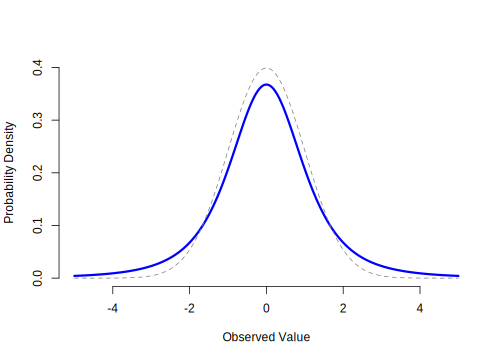
\includegraphics[width=0.66\linewidth]{lsc_files/figure-latex/tdist-1} 

}

\caption{A $t$ distribution with 3 degrees of freedom (solid line). It looks similar to a normal distribution, but it's not quite the same. For comparison purposes, we've plotted a standard normal distribution as the dashed line. Note that the "tails" of the $t$ distribution are "heavier" (i.e., extend further outwards) than the tails of the normal distribution? That's the important difference between the two. }\label{fig:tdist}
\end{figure}

\begin{itemize}
\tightlist
\item
  The \textbf{\emph{\(\chi^2\) distribution}} is another distribution that turns up in lots of different places. The situation in which we'll see it is when doing categorical data analysis (Chapter \ref{chisquare}), but it's one of those things that actually pops up all over the place. When you dig into the maths (and who doesn't love doing that?), it turns out that the main reason why the \(\chi^2\) distribution turns up all over the place is that if you have a bunch of variables that are normally distributed, square their values and then add them up (a procedure referred to as taking a ``sum of squares''), this sum has a \(\chi^2\) distribution. You'd be amazed how often this fact turns out to be useful. Anyway, here's what a \(\chi^2\) distribution looks like: Figure \ref{fig:chisqdist}.
\end{itemize}

\begin{figure}

{\centering 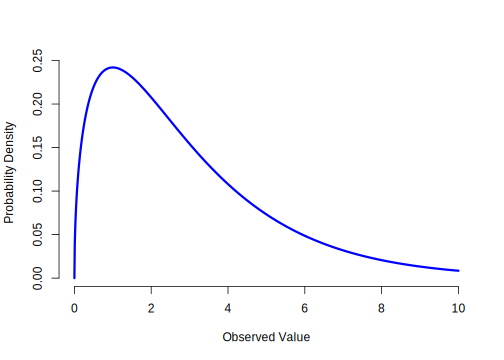
\includegraphics[width=0.66\linewidth]{lsc_files/figure-latex/chisqdist-1} 

}

\caption{A $chi^2$ distribution with 3 degrees of freedom. Notice that the observed values must always be greater than zero, and that the distribution is pretty skewed. These are the key features of a chi-square distribution.}\label{fig:chisqdist}
\end{figure}

\begin{itemize}
\tightlist
\item
  The \textbf{\emph{\(F\) distribution}} looks a bit like a \(\chi^2\) distribution, and it arises whenever you need to compare two \(\chi^2\) distributions to one another. Admittedly, this doesn't exactly sound like something that any sane person would want to do, but it turns out to be very important in real-world data analysis. Remember when we said that \(\chi^2\) turns out to be the key distribution when we're taking a ``sum of squares''? Well, what that means is if you want to compare two different ``sums of squares'', you're probably talking about something that has an \(F\) distribution. Of course, we still haven't given you an example of anything involving a sum of squares, but we will in Chapter \ref{anova}. And that's where we'll run into the \(F\) distribution. Oh, and here's a picture: Figure \ref{fig:Fdist}.
\end{itemize}

\begin{figure}

{\centering 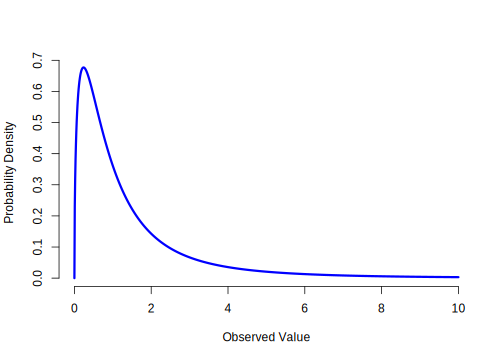
\includegraphics[width=0.66\linewidth]{lsc_files/figure-latex/Fdist-1} 

}

\caption{An $F$ distribution with 3 and 5 degrees of freedom. Qualitatively speaking, it looks pretty similar to a chi-square distribution, but they're not quite the same in general.}\label{fig:Fdist}
\end{figure}

They're all continuous distributions, and they're all closely related to the normal distribution. The key thing for our purposes, however, is not that you have a deep understanding of all these different distributions, nor that you remember the precise relationships between them. The main thing is that you grasp the basic idea that these distributions are all deeply related to one another and to the normal distribution. Later on, we're going to run into data that are normally distributed or at least assumed to be normally distributed. What you have to understand right now is that if you make the assumption that your data are normally distributed, you shouldn't be surprised to see \(\chi^2\), \(t\) and \(F\) distributions popping up all over the place when you start trying to do your data analysis.

\hypertarget{summary-2}{%
\section{Summary}\label{summary-2}}

In this chapter we've talked about probability. We've talked about what probability means, and why statisticians can't agree on what it means. We talked about the rules that probabilities have to obey. And we introduced the idea of a probability distribution, and we spent a good portion of the chapter talking about some of the more important probability distributions that statisticians work with. The section by section breakdown looks like this:

\begin{itemize}
\tightlist
\item
  Probability theory versus statistics (Section \ref{probabilitystats})
\item
  Frequentist versus Bayesian views of probability (Section \ref{probabilitymeaning})
\item
  Basics of probability theory (Section \ref{basicprobability})
\item
  Binomial distribution (Section \ref{binomial}), normal distribution (Section \ref{normal}), and others (Section \ref{otherdists})
\end{itemize}

Many undergraduate psychology classes on statistics skim over this content very quickly, and even the more advanced courses will often ``forget'' to revisit the basic foundations of the field. Most academic psychologists would not know the difference between probability and density; until recently, very few would have been aware of the difference between Bayesian and frequentist probability. However, it's essential to understand these things before moving on to the applications. For example, there are a lot of rules about what you're ``allowed'' to say when making statistical inferences, and many of these can seem arbitrary and weird. However, they start to make sense if you understand this Bayesian/frequentist distinction. Similarly, in Chapter \ref{ttest} we're going to talk about something called the \(t\)-test, and if you really want to have a grasp of the mechanics of the \(t\)-test it really helps to have a sense of what a \(t\)-distribution actually looks like. You get the idea.

\hypertarget{estimation}{%
\chapter{Population, sampling, estimation}\label{estimation}}

As discussed in Chapter \ref{exploringavariable}, the role of descriptive statistics is to concisely summarise what we \emph{do} know. In contrast, inferential statistics aims to ``learn what we do not know from what we do''. Now that we have a foundation in probability theory, we are in a good position to think about the problem of statistical inference. What kinds of things would we like to learn about? And how do we learn them? These questions lie at the heart of inferential statistics and are traditionally divided into two ``big ideas'': estimation and hypothesis testing.

The goal of this chapter is to introduce sampling theory first because, later on, estimation theory doesn't make sense until you understand sampling.

\hypertarget{srs}{%
\section{Samples, populations and sampling}\label{srs}}

\emph{All} learning requires you to make assumptions. Accepting this is true, our first task is to come up with some fairly general assumptions about data that make sense. If probability theory is the foundation upon which all statistical theory builds, \textbf{sampling theory} is the frame around which you can build the rest of the house. It plays a massive role in specifying the assumptions upon which your statistical inferences rely. And to talk about ``making inferences'' the way statisticians think about it, we need to be a bit more explicit about what it is that we're drawing inferences \emph{from} (the sample) and what it is that we're drawing inferences \emph{about} (the population).

In almost every situation of interest, we have a \textbf{sample} of data available to us as researchers. We might have run an experiment with some number of participants; a polling company might have phoned some number of people to ask questions about voting intentions; etc. Regardless: the data set available to us is finite and incomplete. We can't possibly get every person in the world to do our experiment; a polling company doesn't have the time or the money to ring up every voter in the country etc. In our earlier discussion of descriptive statistics (Chapter \ref{exploringavariable}, this sample was the only thing we were interested in. Our only goal was to find ways of describing, summarising and graphing that sample. This is about to change.

\hypertarget{pop}{%
\subsection{Defining a population}\label{pop}}

A sample is a tangible thing. You can open up a data file, and there you have data from your sample. A \textbf{population}, on the other hand, is a more abstract idea. It refers to the set of all possible people, or all possible observations, that you want to draw conclusions about and is generally \emph{much} bigger than the sample. In an ideal world, the researcher would begin the study with a clear idea of what the population of interest is since the process of designing a study and testing hypotheses about the data that it produces does depend on the population about which you want to make statements. However, that doesn't always happen in practice: usually, the researcher has a relatively vague idea of what the population is and designs the study as best they can on that basis.

Sometimes it's easy to state the population of interest. For instance, in the ``polling company'' example that opened the chapter, the population consisted of all voters enrolled at the time of the study -- millions of people. The sample was a set of 1000 people belonging to that population. In most cases, the situation is much less simple. Determining the population of interest in a typical psychological experiment is a bit more complicated. Suppose we run an experiment using 100 undergraduate students as our participants. Our goal, as cognitive scientists, is to try to learn something about how the mind works. So, which of the following would count as ``the population'':

\begin{itemize}
\tightlist
\item
  All of the undergraduate psychology students at the University of Adelaide?
\item
  Undergraduate psychology students in general, anywhere in the world?
\item
  Australians currently living?
\item
  Australians of similar ages to my sample?
\item
  Anyone currently alive?
\item
  Any human being, past, present or future?
\item
  Any biological organism with sufficient intelligence operating in a terrestrial environment?
\item
  Any intelligent being?
\end{itemize}

Each of these defines a real group of mind-possessing entities, all of which might be of interest, and it's not clear which one should be the true population of interest.

\hypertarget{simple-random-samples}{%
\subsection{Simple random samples}\label{simple-random-samples}}

\begin{figure}

{\centering 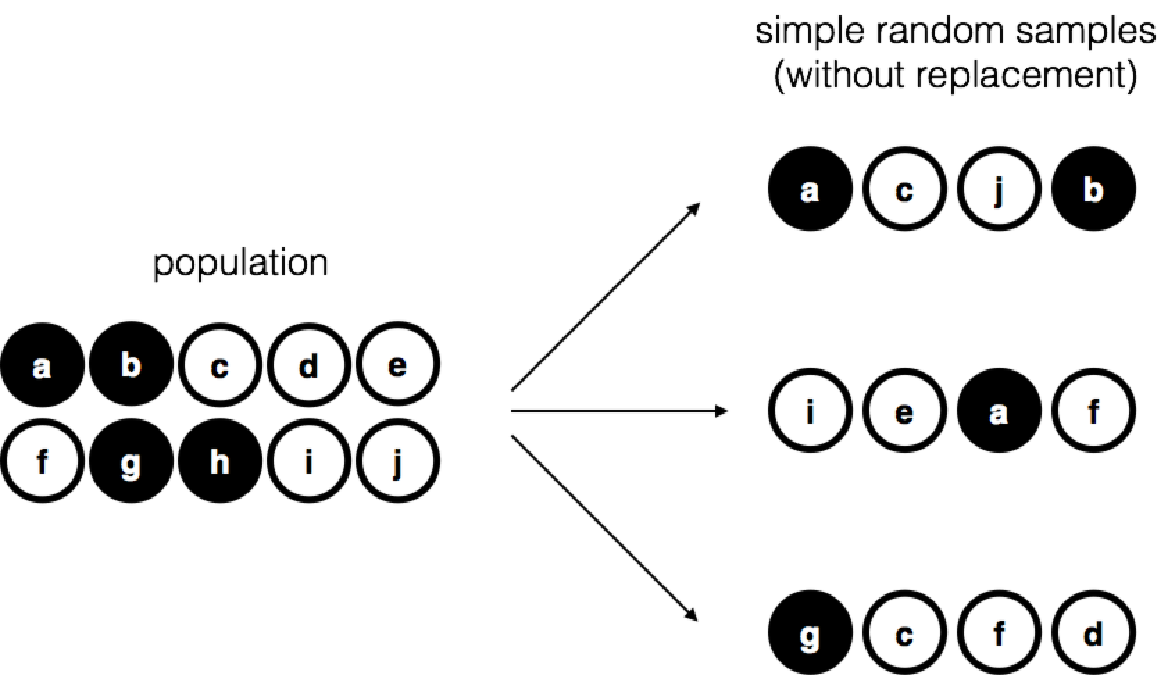
\includegraphics[width=0.66\linewidth]{resources/image/srs1} 

}

\caption{Simple random sampling without replacement from a finite population}\label{fig:srs1}
\end{figure}

Irrespective of how we define the population, the critical point is that the sample is a subset of the population. Our goal is to use our knowledge of the sample to draw inferences about the properties of the population. The relationship between the two depends on the \emph{procedure} by which the sample was selected. This procedure is referred to as a \textbf{sampling method}, and it is important to understand why it matters.

To keep things simple, let's imagine that we have a bag containing 10 chips. Each chip has a unique letter printed on it, so we can distinguish between the 10 chips. The chips come in two colours, black and white. This set of chips is the population of interest, and it is depicted graphically on the left of Figure \ref{fig:srs1}. As you can see from looking at the picture, there are 4 black chips and 6 white chips, but of course, in real life, we wouldn't know that unless we looked in the bag. Now imagine you run the following ``experiment'': you shake up the bag, close your eyes, and pull out 4 chips without putting any of them back into the bag. First out comes the \(a\) chip (black), then the \(c\) chip (white), then \(j\) (white) and then finally \(b\) (black). If you wanted, you could then put all the chips back in the bag and repeat the experiment, as depicted on the right-hand side of Figure \ref{fig:srs1}. Each time you get different results, but the procedure is identical in each case. The fact that the same procedure can lead to different results each time, we refer to it as a \emph{random} process.\footnote{The proper mathematical definition of randomness is extraordinarily technical and way beyond the scope of this book. We'll be non-technical here and say that a process has an element of randomness to it whenever it is possible to repeat it and get different answers each time.} However, because we shook the bag before pulling any chips out, it seems reasonable to think that every chip has the same chance of being selected. A procedure in which every member of the population has the same chance of being selected is called a \textbf{simple random sample}. The fact that we did \emph{not} put the chips back in the bag after pulling them out means that you can't observe the same thing twice, and in such cases, the observations are said to have been sampled \textbf{without replacement}.

To help make sure you understand the importance of the sampling procedure, consider an alternative way the experiment could have been run. Suppose a 5-year-old had opened the bag and decided to pull out four black chips without putting any of them back in the bag. This \emph{biased} sampling scheme is depicted in Figure \ref{fig:brs}. Now consider the evidentiary value of seeing 4 black chips and 0 white chips. Clearly, it depends on the sampling scheme. If you know that the sampling scheme is biased to select only black chips, then a sample that consists of only black chips doesn't tell you very much about the population! For this reason, statisticians really like it when a data set can be considered a simple random sample, because it makes the data analysis \emph{much} easier.

\begin{figure}

{\centering 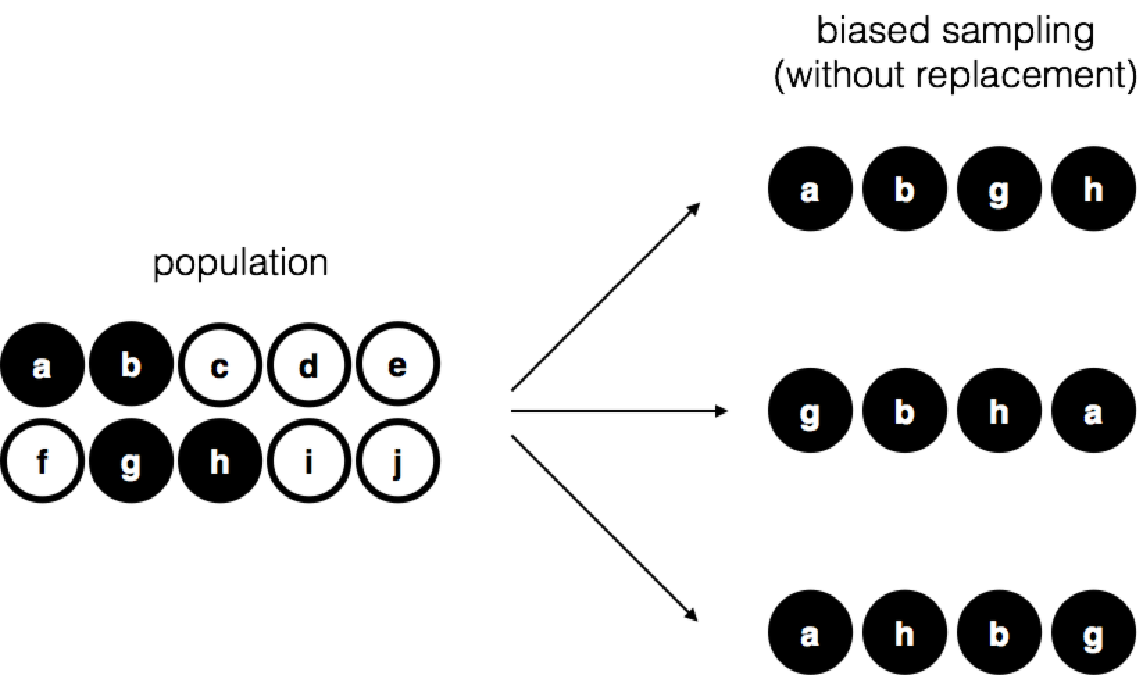
\includegraphics[width=0.66\linewidth]{resources/image/brs} 

}

\caption{Biased sampling without replacement from a finite population}\label{fig:brs}
\end{figure}



\begin{figure}

{\centering 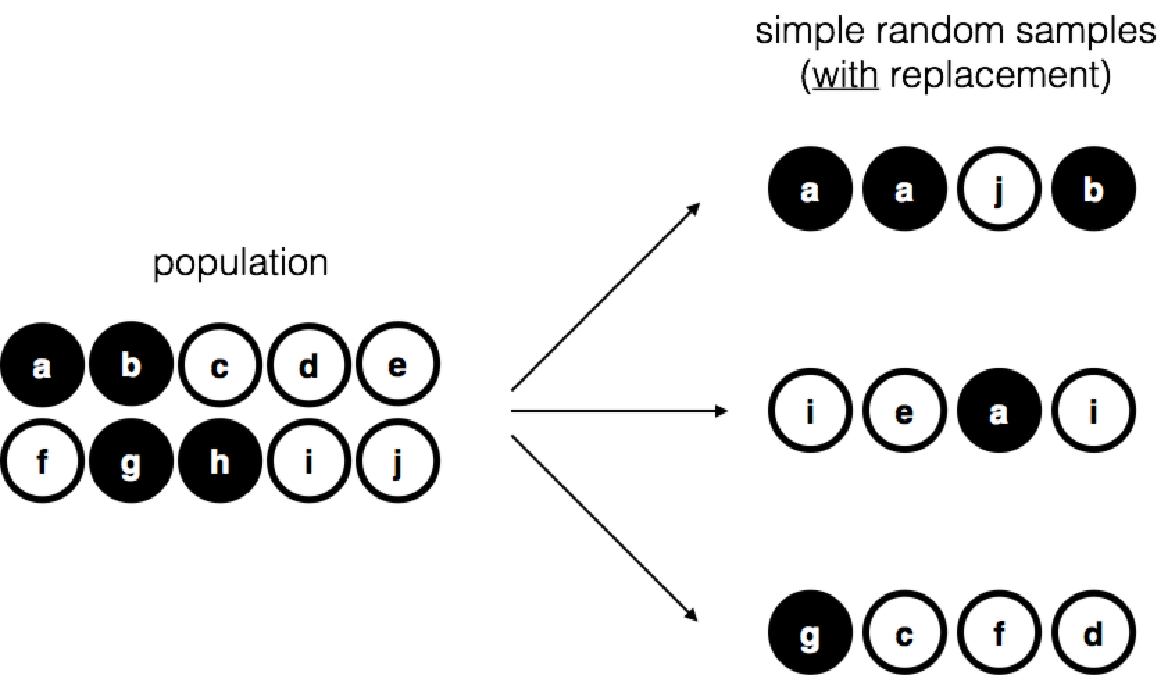
\includegraphics[width=0.66\linewidth]{resources/image/srs2} 

}

\caption{Simple random sampling \emph{with} replacement from a finite population}\label{fig:srs2}
\end{figure}

A third procedure is worth mentioning. We close our eyes, shake the bag, and pull out a chip this time. This time, however, we record the observation and then put the chip back in the bag. Again we close our eyes, shake the bag, and pull out a chip. We then repeat this procedure until we have 4 chips. Data sets generated in this way are still simple random samples, but because we put the chips back in the bag immediately after drawing them, it is referred to as a sample \textbf{with replacement}. The difference between this situation and the first one is that it is possible to observe the same population member multiple times, as illustrated in Figure \ref{fig:srs2}.

Most psychology experiments tend to be sampling without replacement because the same person is not allowed to participate in the experiment twice. However, most statistical theories are based on the assumption that the data arise from a simple random sample \emph{with} replacement. In real life, this very rarely matters. If the population of interest is large (e.g., has much more than 10 entities!), the difference between sampling with and without replacement is too small to be concerned with. The difference between simple random samples and biased samples, on the other hand, is not such an easy thing to dismiss.

\hypertarget{most-samples-are-not-simple-random-samples}{%
\subsection{Most samples are not simple random samples}\label{most-samples-are-not-simple-random-samples}}

As you can see from the list of possible populations above, it is almost impossible to obtain a simple random sample from most populations of interest. A thorough discussion of other types of sampling schemes is beyond the scope of this book, but to give you a sense of what's out there, here's a list of a few of the more important ones:

\begin{itemize}
\tightlist
\item
  \textbf{Stratified sampling}. Suppose your population can be divided into several subpopulations, or \emph{strata}. Perhaps you're running a study at different sites, for example. Instead of trying to sample randomly from the population as a whole, you try to collect a separate random sample from each stratum. Stratified sampling is sometimes easier to do than simple random sampling, especially when the population is already divided into distinct strata. It can also be more efficient than simple random sampling, especially when some subpopulations are rare. For instance, when studying schizophrenia, it would be much better to divide the population into two\footnote{Nothing in life is that simple: there's not an obvious division of people into binary categories like ``schizophrenic'' and ``not schizophrenic''. But this isn't a clinical psychology text, so please forgive a few simplifications here and there.} strata (schizophrenic and not-schizophrenic), and then sample an equal number of people from each group. If you selected people randomly, you would get so few schizophrenic people in the sample that your study would be useless. This specific kind of stratified sampling is called \emph{oversampling} because it deliberately attempts to over-represent rare groups.
\item
  \textbf{Snowball sampling} is a technique that is especially useful when sampling from a ``hidden'' or hard-to-access population and is widespread in social sciences. For instance, suppose the researchers want to conduct an opinion poll among transgender people. The research team might only have contact details for a few trans folks, so the survey starts by asking them to participate (stage 1). At the end of the survey, the participants are asked to provide contact details for other people who might want to participate. In stage 2, those new contacts are surveyed. The process continues until the researchers have sufficient data. The advantage of snowball sampling is that it lets access data in situations that might otherwise be impossible to get any. On the statistical side, the main disadvantage is that the sample is highly non-random. On the real-life side, the disadvantage is that the procedure can be unethical if not handled well because hidden populations are often hidden for a reason. I chose transgender people as an example here to highlight this. If you weren't careful, you might end up outing people who don't want to be outed (very, very bad form), and even if you don't make that mistake, it can still be intrusive to use people's social networks to study them. It's undoubtedly tough to get people's informed consent \emph{before} contacting them, yet in many cases, the simple act of contacting them and saying, ``hi, we want to study you'', can be hurtful. Social networks are complex, and just because you can use them to get data doesn't always mean you should.
\item
  \emph{Convenience sampling} is more or less what it sounds. The samples are chosen in a way that is convenient to the researcher, and not selected at random from the population of interest. Snowball sampling is one type of convenience sampling, but there are many others. A common example in psychology are studies that rely on undergraduate psychology students. These samples are generally non-random in two respects: firstly, reliance on undergraduate psychology students automatically means that your data are restricted to a single subpopulation. Secondly, the students usually get to pick which studies they participate in, so the sample is a self-selected subset of psychology students, not a randomly selected subset. In real life, most studies are convenience samples of one form or another. This is sometimes a severe limitation, but not always.
\end{itemize}

\hypertarget{how-much-does-it-matter-if-you-dont-have-a-simple-random-sample}{%
\subsection{How much does it matter if you don't have a simple random sample?}\label{how-much-does-it-matter-if-you-dont-have-a-simple-random-sample}}

Okay, so real-world data collection tends not to involve nice simple random samples. Does that matter? A little thought should make it clear to you that it \emph{can} matter if your data are not a simple random sample: think about the difference between Figures \ref{fig:srs1} and \ref{fig:brs}. However, it's not quite as bad as it sounds. Some types of biased samples are entirely unproblematic. For instance, when using a stratified sampling technique, you \emph{know} what the bias is because you created it deliberately, often to \emph{increase} the effectiveness of your study. So in those situations, it's not a problem. Also, there are statistical techniques that you can use to adjust for the biases you've introduced, but they are not covered in this book.

More generally, it's important to remember that random sampling is a means to an end, not the end itself. Let's assume you've relied on a convenience sample; as such, you can assume it's biased. A bias in your sampling method is only a problem if it causes you to draw the wrong conclusions. When viewed from that perspective, I'd argue that we don't need the sample to be randomly generated in \emph{every} respect: we only need it to be random for the psychologically-relevant phenomenon of interest.

Suppose we're doing a study looking at working memory capacity. In study 1, we can sample randomly from all human beings currently alive, with one exception: we can only sample people born on a Monday. In study 2, we are able to sample randomly from the Australian population. We want to generalise my results to the population of all living humans. Which study is better? The answer, obviously, is study 1. Why? Because we have no reason to think that being ``born on a Monday'' has any interesting relationship to working memory capacity. In contrast, we can think of several reasons why ``being Australian'' might matter. Australia is a wealthy, industrialised country with a very well-developed education system. People growing up in that system will have had life experiences much more similar to the experiences of the people who designed the tests for working memory capacity. This shared experience might easily translate into similar beliefs about how to ``take a test'', a shared assumption about how psychological experimentation works, and so on. These things might actually matter. For instance, the ``test-taking'' style might have taught the Australian participants how to direct their attention exclusively on somewhat abstract test materials relative to people who haven't grown up in a similar environment, leading to a misleading picture of working memory capacity.

There are two points hidden in this discussion. Firstly, when designing your studies, you must consider what population you care about and try hard to sample in a way appropriate to that population. In practice, you're usually forced to put up with a ``sample of convenience'' (e.g., psychology lecturers sample psychology students because that's the least expensive way to collect data, and our coffers aren't exactly overflowing with gold). But you should at least spend some time thinking about the dangers of this practice.

Secondly, if you're criticising someone else's study because they've used a sample of convenience rather than laboriously sampling randomly from the entire human population, at least have the courtesy to offer a specific theory as to \emph{how} this might have distorted the results. Remember, everyone in science knows this issue and does what they can to alleviate it. Merely pointing out that ``the study only included people from group BLAH'' is entirely unhelpful and borders on insulting the researchers, who are, \emph{of course}, aware of the issue. They just don't happen to own the infinite supply of time and money required to construct the perfect sample. In short, if you want to offer a responsible critique of the sampling process, then be \emph{helpful}.

\hypertarget{population-parameters-and-sample-statistics}{%
\subsection{Population parameters and sample statistics}\label{population-parameters-and-sample-statistics}}

Let's consider a slightly different case by setting aside the thorny methodological issues associated with obtaining a random sample and my rather unfortunate tendency to rant about lazy methodological criticism. Up to this point, we have been talking about populations the way a scientist might: a population might be a group of people to a psychologist; to an ecologist, a population might be a group of bears. In most cases, the populations that scientists care about are tangible things that exist in the real world. Statisticians are interested in real-world data and actual science the same way scientists are. On the other hand, they also operate in the realm of pure abstraction as mathematicians do. Consequently, statistical theory tends to be a bit abstract in how a population is defined. In much the same way that psychological researchers operationalise our abstract theoretical ideas in terms of concrete measurements (Section \ref{measurement}, statisticians operationalise the concept of a ``population'' in terms of mathematical objects that they know how to work with. You've already come across these objects in Chapter \ref{probability}: they're called \textbf{probability distributions}.

The idea is quite simple. Let's say we're talking about IQ scores. To a psychologist, the population of interest is a group of actual humans with IQ scores. A statistician ``simplifies'' this by operationally defining the population as the probability distribution depicted in Figure \ref{fig:IQdista}. IQ tests are designed so that the average IQ is 100, the standard deviation of IQ scores is 15, and the distribution of IQ scores is normal. These values are referred to as the \textbf{population parameters} because they are characteristics of the entire population. That is, we say that the population mean \(\mu\) is 100, and the population standard deviation \(\sigma\) is 15.

\begin{figure}

{\centering 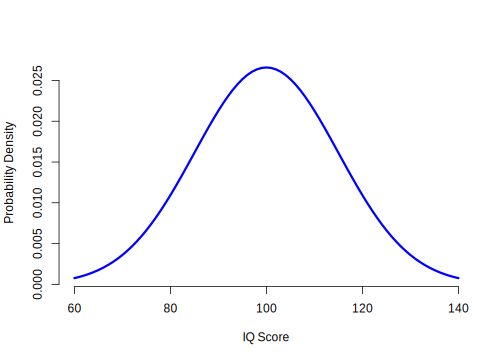
\includegraphics[width=0.66\linewidth]{resources/image/IQdista} 

}

\caption{The population distribution of IQ scores.}\label{fig:IQdista}
\end{figure}

Now let us run an experiment. We select 100 people at random and administer an IQ test, giving us a simple random sample from the population. The sample would consist of a collection of numbers like this:

\begin{verbatim}
 106 101 98 80 74 ... 107 72 100
\end{verbatim}

\begin{figure}

{\centering 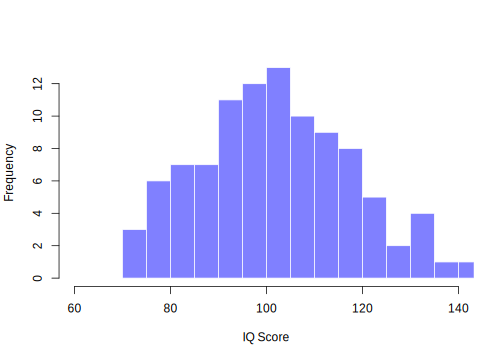
\includegraphics[width=0.66\linewidth]{resources/image/IQdistb} 

}

\caption{A sample of 100 observations drawn from the population distribution of IQ scores.}\label{fig:IQdistb}
\end{figure}

Each IQ score is sampled from a normal distribution with a mean of 100 and a standard deviation of 15. So if we plot a histogram of the sample, we get something like the one shown in Figure \ref{fig:IQdistb}. As you can see, the histogram is \emph{roughly} the proper shape, but it's a very crude approximation to the actual population distribution shown in Figure \ref{fig:IQdista}. When calculating the mean of the sample, we get a number that is relatively close to the population mean of 100 but not identical. In this case, it turns out that the people in the sample have a mean IQ of 98.5, and the standard deviation of their IQ scores is 15.9. These \textbf{sample statistics} are properties of our data set, and although they are reasonably similar to the actual population values, they are not the same.

In general, sample statistics are the things you can calculate from your data set, and the population parameters are the things you want to learn about.

\hypertarget{lawlargenumbers}{%
\section{The law of large numbers}\label{lawlargenumbers}}

In the previous section, we discussed the results of one fictitious IQ experiment with a sample size of \(N=100\). The results were somewhat encouraging: the true population mean was 100, and the sample mean of 98.5 was a reasonable approximation. In many scientific studies, that level of precision is perfectly acceptable, but in other situations, you need to be much more precise. If we want our sample statistics to be much closer to the population parameters, what can we do about it?

The obvious answer is to collect more data. Suppose that we ran a much larger experiment, this time measuring the IQs of 10,000 people. For an experiment with a sample size of \texttt{n\ =\ 10000}, and a population with \texttt{mean\ =\ 100} and \texttt{sd\ =\ 15}, we get the following distribution:

\begin{figure}

{\centering 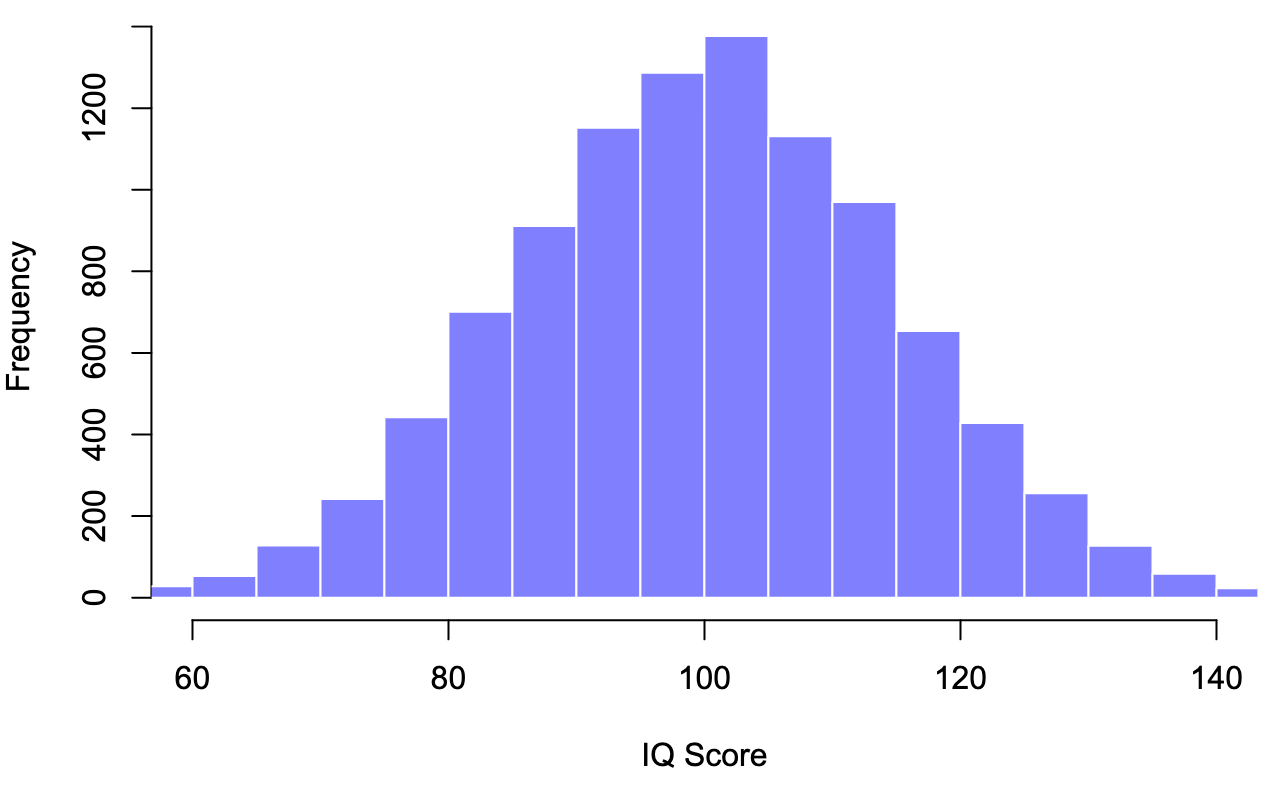
\includegraphics[width=0.66\linewidth]{resources/image/IQdistc} 

}

\caption{A sample of 10,000 observations drawn from the population distribution of IQ scores.}\label{fig:IQdistc}
\end{figure}

Large samples generally give you better information. It feels silly saying it because it's so bloody obvious that it shouldn't need to be said. It's such an obvious point that when Jacob Bernoulli -- one of the founders of probability theory -- formalised this idea back in 1713, he was kind of a jerk about it. Here's how he described the fact that we all share this intuition:

\begin{quote}
\emph{For even the most stupid of men, by some instinct of nature, by himself and without any instruction (which is a remarkable thing), is convinced that the more observations have been made, the less danger there is of wandering from one's goal.} Stigler (\protect\hyperlink{ref-Stigler1986}{1986})
\end{quote}

Okay, so the passage comes across as a bit condescending (not to mention sexist), but his main point is correct: it really does feel evident that more data will give you better answers. The question is, why is this so? Not surprisingly, this intuition we all share is correct, and statisticians refer to it as the \textbf{law of large numbers}. The law of large numbers is a mathematical law that applies to many different sample statistics, but the simplest way to think about it is as a law about averages. The sample mean is the most obvious example of a statistic that relies on averaging (because that's what the mean is -- an average), so let's look at that.

When applied to the sample mean, the law of large numbers states that as the sample gets larger, the sample mean tends to get closer to the true population mean. Or, to say it a little bit more precisely, as the sample size ``approaches'' infinity (written as \(N \rightarrow \infty\)) the sample mean approaches the population mean (\(\bar{X} \rightarrow \mu\)).\footnote{Technically, the law of large numbers pertains to any sample statistic that can be described as an average of independent quantities. That's certainly true for the sample mean. However, it's also possible to write many other sample statistics as averages of one form or another. The variance of a sample, for instance, can be rewritten as an average and so is subject to the law of large numbers. The minimum value of a sample, however, cannot be written as an average of anything and is therefore not governed by the law of large numbers.}

You won't be subject to proof that the law of large numbers is true, but it's one of the most important tools for statistical theory. The law of large numbers is the thing we can use to justify our belief that collecting more and more data will eventually lead us to the truth. For any particular data set, the sample statistics that we calculate from it will be wrong, but the law of large numbers tells us that if we keep collecting more data, those sample statistics will tend to get closer and closer to the true population parameters.

\hypertarget{samplesandclt}{%
\section{Sampling distributions and the central limit theorem}\label{samplesandclt}}

The law of large numbers is a potent tool, but it will not be good enough to answer all our questions. Among other things, it gives us a ``long-run guarantee''. In the long run, if we could collect an infinite amount of data, then the law of large numbers guarantees that our sample statistics will be correct. But as John Maynard Keynes famously argued in economics, a long-run guarantee is of little use in real life:

\begin{quote}
\emph{{[}The{]} long run is a misleading guide to current affairs. In the long run we are all dead. Economists set themselves too easy, too useless a task, if in tempestuous seasons they can only tell us, that when the storm is long past, the ocean is flat again.} Keynes (\protect\hyperlink{ref-Keynes1923}{1923})
\end{quote}

As in economics, so too in psychology and statistics. It is not enough to know that we will \emph{eventually} arrive at the right answer when calculating the sample mean. Knowing that an infinitely large data set will tell me the exact value of the population mean is cold comfort when my \emph{actual} data set has a sample size of \(N=100\). In real life, then, we must know something about the behaviour of the sample mean when it is calculated from a more modest data set!

\hypertarget{samplingdists}{%
\subsection{Sampling distribution of the mean}\label{samplingdists}}

With this in mind, let's abandon the idea that our studies will have sample sizes of 10000 and consider a very modest experiment indeed. This time around, we'll sample \(N=5\) people and measure their IQ scores.

\begin{verbatim}
90  82  94  99  110
\end{verbatim}

The mean IQ in this sample turns out to be exactly 95. Not surprisingly, this is much less accurate than the previous experiment. Now imagine that we decided to \textbf{replicate} the experiment. That is, we repeat the procedure as closely as possible: randomly sample 5 new people and measure their IQ.

\begin{verbatim}
78  88  111  111  117
\end{verbatim}

This time around, the mean IQ in the sample is 101.

If we repeat the experiment 10 times, we obtain the results shown in Table \ref{tab:replications}, and as you can see, the sample mean varies from one replication to the next.

\begin{table}

\caption{\label{tab:replications}Ten replications of the IQ experiment, each with a sample size of $N=5$.}
\centering
\begin{tabular}[t]{lcccccc}
\toprule
Replication & Person 1 & Person 2 & Person 3 & Person 4 & Person 5 & Sample Mean\\
\midrule
Replication 1 & 90 & 82 & 94 & 99 & 110 & 95.0\\
Replication 2 & 78 & 88 & 111 & 111 & 117 & 101.0\\
Replication 3 & 111 & 122 & 91 & 98 & 86 & 101.6\\
Replication 4 & 98 & 96 & 119 & 99 & 107 & 103.8\\
Replication 5 & 105 & 113 & 103 & 103 & 98 & 104.4\\
\addlinespace
Replication 6 & 81 & 89 & 93 & 85 & 114 & 92.4\\
Replication 7 & 100 & 93 & 108 & 98 & 133 & 106.4\\
Replication 8 & 107 & 100 & 105 & 117 & 85 & 102.8\\
Replication 9 & 86 & 119 & 108 & 73 & 116 & 100.4\\
Replication 10 & 95 & 126 & 112 & 120 & 76 & 105.8\\
\bottomrule
\end{tabular}
\end{table}

Suppose we decided to keep going in this fashion, replicating this ``five IQ scores'' experiment repeatedly. Every time we replicate the experiment, we write down the sample mean. Over time, we should be amassing a new data set in which every experiment generates a single data point. The first 10 observations from the data set are the sample means listed in Table \ref{tab:replications}, so our data set starts out like this:

\begin{verbatim}
95.0 101.0 101.6 103.8 104.4 ...
\end{verbatim}

What if we should continue like this for 10,000 replications and then draw a histogram? As Figure \ref{fig:sampdistmean} illustrates, the average of 5 IQ scores is usually between 90 and 110. But more importantly, what it highlights is that if we replicate an experiment over and over again, what we end up with is a \emph{distribution} of sample means! This distribution has a particular name in statistics: the \textbf{sampling distribution of the mean}.

Sampling distributions are another important theoretical idea in statistics, and they're crucial for understanding the behaviour of small samples. For instance, when we ran the very first ``five IQ scores'' experiment, the sample mean turned out to be 95. What the sampling distribution in Figure \ref{fig:sampdistmean} tells us, though, is that the ``five IQ scores'' experiment is not very accurate. If we repeat the experiment, the sampling distribution tells me that we can expect to see a sample mean anywhere between 80 and 120.



\begin{figure}

{\centering 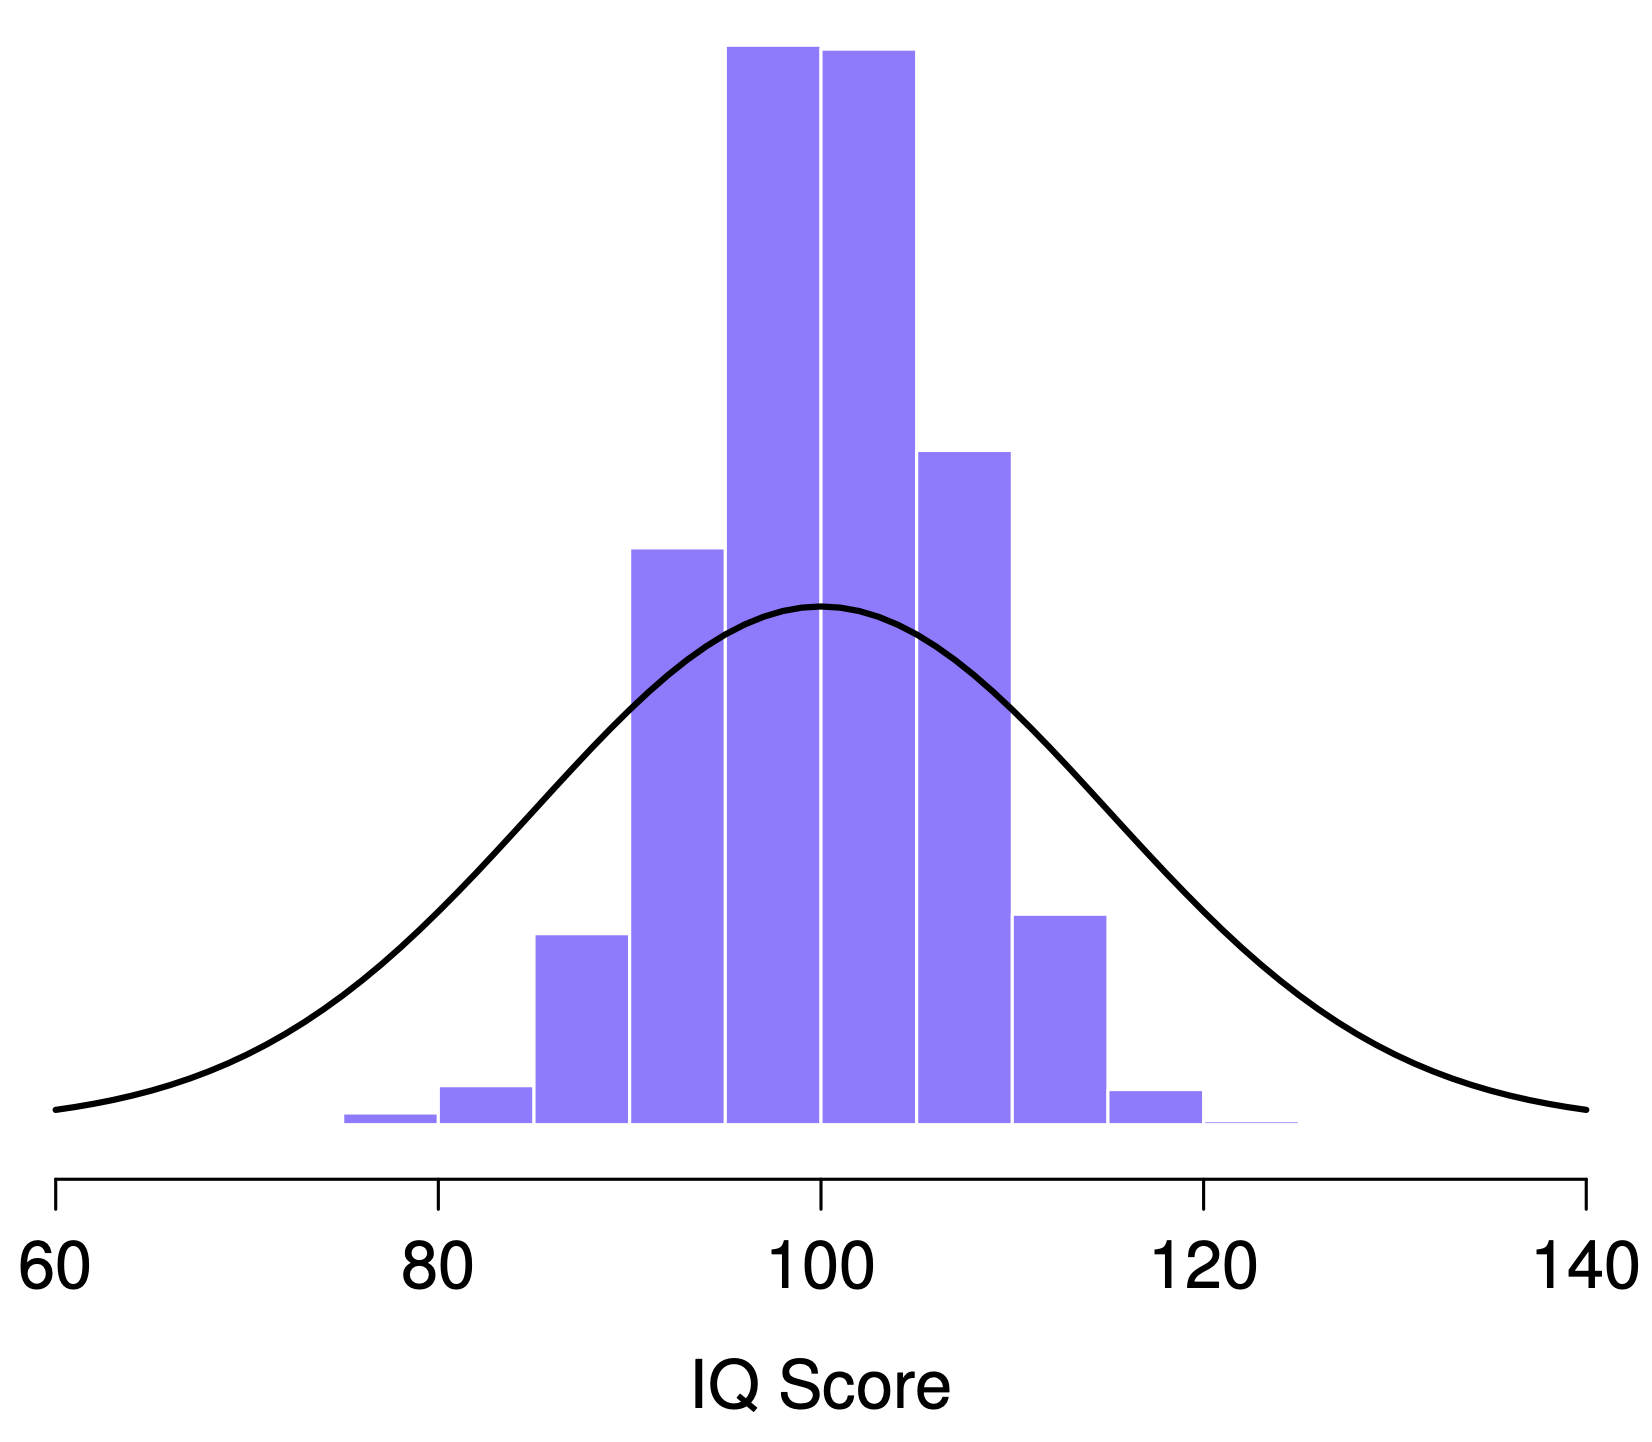
\includegraphics[width=0.66\linewidth]{resources/image/sampleDist4} 

}

\caption{The sampling distribution of the mean for the ``five IQ scores experiment''. If you sample 5 people at random and calculate their \emph{average} IQ, you'll almost certainly get a number between 80 and 120, even though there are quite a lot of individuals who have IQs above 120 or below 80. For comparison, the black line plots the population distribution of IQ scores.}\label{fig:sampdistmean}
\end{figure}

\hypertarget{sampling-distributions-exist-for-any-sample-statistic}{%
\subsection{Sampling distributions exist for any sample statistic!}\label{sampling-distributions-exist-for-any-sample-statistic}}

One thing to remember when thinking about sampling distributions is that \emph{any} sample statistic you might care to calculate has a sampling distribution. For example, suppose that each time we replicated the ``five IQ scores'' experiment, we wrote down the largest IQ score in the experiment. This would give us a data set that started out like this:

\begin{verbatim}
110 117 122 119 113 ... 
\end{verbatim}

Doing this over and over again would give a very different sampling distribution, namely the \emph{sampling distribution of the maximum}. The sampling distribution of the maximum of 5 IQ scores is shown in Figure \ref{fig:sampdistmax}. Not surprisingly, if you pick 5 people at random and then find the person with the highest IQ score, they're going to have an above-average IQ. Most of the time, you'll end up with someone whose IQ is measured in the 100 to 140 range.



\begin{figure}

{\centering 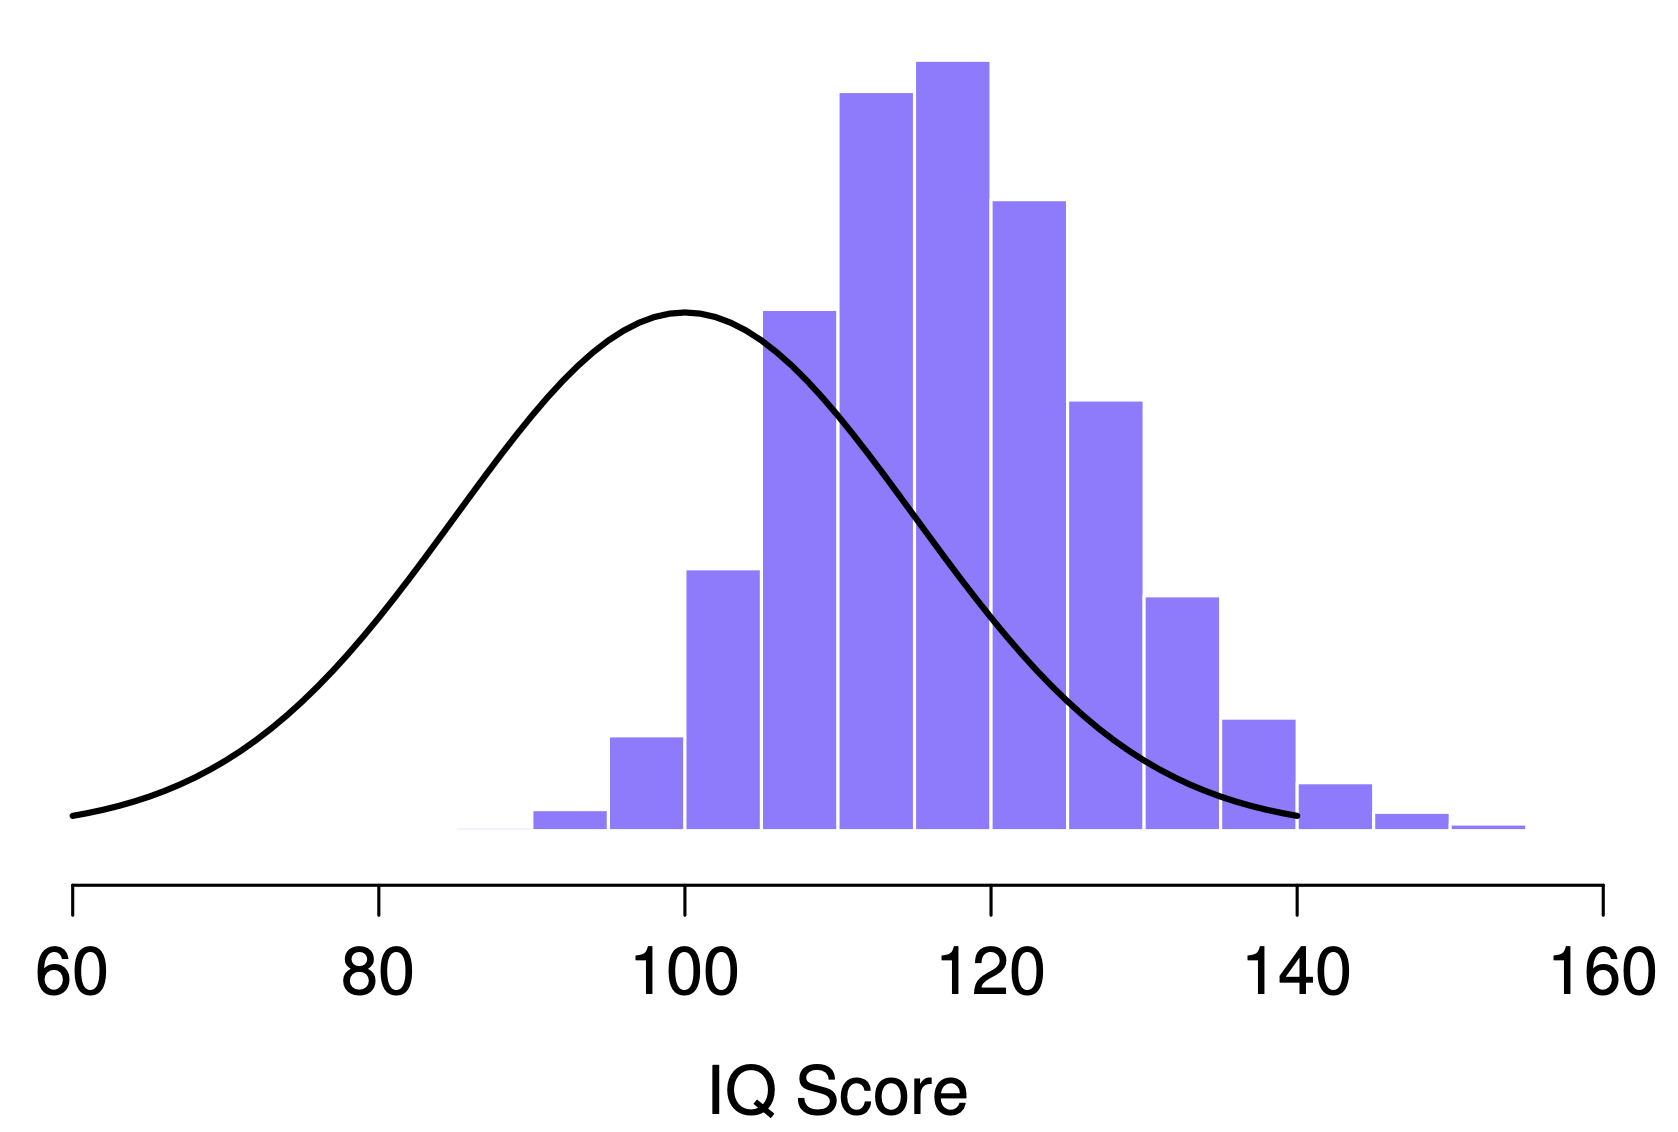
\includegraphics[width=0.66\linewidth]{resources/image/sampleDistMax} 

}

\caption{The sampling distribution of the \emph{maximum} for the ``five IQ scores experiment''. If you sample 5 people at random and select the one with the highest IQ score, you'll probably see someone with an IQ between 100 and 140.}\label{fig:sampdistmax}
\end{figure}

\hypertarget{clt}{%
\subsection{The central limit theorem}\label{clt}}

Here's an illustration of how the sampling distribution of the mean depends on the sample size. In each panel, there are 10,000 generated samples of IQ data and the mean IQ observed within each set. The histograms in these plots show the distribution of these means (i.e.~the sampling distribution of the mean). Each individual IQ score was drawn from a normal distribution with mean 100 and standard deviation 15, which is shown as the solid black line).

\begin{figure}

{\centering 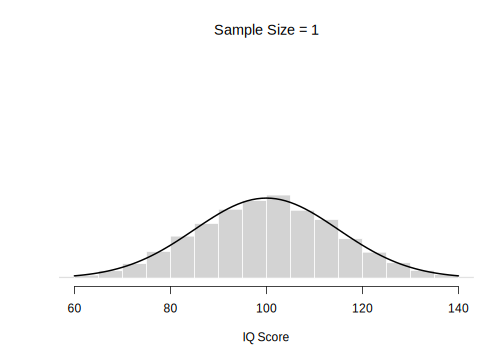
\includegraphics[width=0.66\linewidth]{lsc_files/figure-latex/IQsampa-1} 

}

\caption{Each data set contained only a single observation, so the mean of each sample is just one person's IQ score. As a consequence, the sampling distribution of the mean is of course identical to the population distribution of IQ scores.}\label{fig:IQsampa}
\end{figure}

\begin{figure}

{\centering \includegraphics[width=0.66\linewidth]{lsc_files/figure-latex/IQsampb-1} 

}

\caption{When we raise the sample size to 2, the mean of any one sample tends to be closer to the population mean than a one person's IQ score, and so the histogram (i.e., the sampling distribution) is a bit narrower than the population distribution.}\label{fig:IQsampb}
\end{figure}

\begin{figure}

{\centering \includegraphics[width=0.66\linewidth]{lsc_files/figure-latex/IQsampc-1} 

}

\caption{By the time we raise the sample size to 10, we can see that the distribution of sample means tend to be fairly tightly clustered around the true population mean.}\label{fig:IQsampc}
\end{figure}

At this point, you have a pretty good sense of what sampling distributions are, particularly the sampling distribution of the mean. In this section, let us talk about how the sampling distribution of the mean changes as a function of sample size. Intuitively, you already know part of the answer: if you only have a few observations, the sample mean is likely to be quite inaccurate: if you replicate a small experiment and recalculate the mean, you'll get a very different answer. In other words, the sampling distribution is quite broad. If you replicate a large experiment and recalculate the sample mean, you'll probably get the same answer you got last time, so the sampling distribution will narrow. You can see this visually in Figures \ref{fig:IQsampa}, \ref{fig:IQsampb} and \ref{fig:IQsampc}: the bigger the sample size, the narrower the sampling distribution gets. We can quantify this effect by calculating the standard deviation of the sampling distribution, which is referred to as the \textbf{standard error}. The standard error of a statistic is often denoted SE, and since we're usually interested in the standard error of the sample \emph{mean}, we often use the acronym SEM. As you can see just by looking at the picture, as the sample size \(N\) increases, the SEM decreases.

However, there's something we've been glossing over so far. All examples up to this point have been based on the ``IQ scores'' experiments. And because IQ scores are roughly normally distributed, we've assumed that the population distribution is normal. What if it isn't normal? What happens to the sampling distribution of the mean? The remarkable thing is this: no matter what shape your population distribution is, as \(N\) increases the sampling distribution of the mean starts to look more like a normal distribution.

To give you a sense of this, let's run some simulations. We start with the ``ramped'' distribution shown in the histogram in Figure \ref{fig:cltdemo}. As you can see by comparing the triangular-shaped histogram to the bell curve plotted by the black line, the population distribution doesn't look very much like a normal distribution at all. Next, let us simulate the results of a large number of experiments. In each experiment, we draw \(N=2\) samples from this distribution and then calculate the sample mean. Figure \ref{fig:cltdemo} panel b plots the histogram of these sample means (i.e.~the sampling distribution of the mean for \(N=2\)). This time, the histogram produces a \(\cap\)-shaped distribution: it's still not normal, but it's a lot closer to the black line than the population distribution in Figure \ref{fig:cltdemo} panel a. When we increase the sample size to \(N=4\), the sampling distribution of the mean is very close to normal (Figure \ref{fig:cltdemo} panel c), and by the time we reach a sample size of \(N=8\) it's almost perfectly normal. In other words, as long as your sample size isn't tiny, the sampling distribution of the mean will be approximately normal no matter what your population distribution looks like!

\begin{figure}

{\centering \includegraphics[width=0.45\linewidth]{resources/image/cltDemo-a} \includegraphics[width=0.45\linewidth]{resources/image/cltDemo-b} \includegraphics[width=0.45\linewidth]{resources/image/cltDemo-c} \includegraphics[width=0.45\linewidth]{resources/image/cltDemo-d} 

}

\caption{A demonstration of the central limit theorem. In the top-left panel, we have a non-normal population distribution; and the consecutive panels show the sampling distribution of the mean for samples of size 2, 4 and 8, for data drawn from the distribution in panel a. As you can see, even though the original population distribution is non-normal, the sampling distribution of the mean becomes pretty close to normal by the time you have a sample of even 4 observations. }\label{fig:cltdemo}
\end{figure}

Based on these figures, it seems like we have evidence for all of the following claims about the sampling distribution of the mean:

\begin{itemize}
\tightlist
\item
  The mean of the sampling distribution is the same as the mean of the population
\item
  The standard deviation of the sampling distribution (i.e., the standard error) gets smaller as the sample size increases
\item
  The shape of the sampling distribution becomes normal as the sample size increases
\end{itemize}

As it happens, not only are all of these statements true, there is a very famous theorem in statistics that proves all three of them, known as the \textbf{central limit theorem}. Among other things, the central limit theorem tells us that if the population distribution has mean \(\mu\) and standard deviation \(\sigma\), then the sampling distribution of the mean also has mean \(\mu\), and the standard error of the mean is
\[
\mbox{SEM} = \frac{\sigma}{ \sqrt{N} }
\]

Because we divide the population standard devation \(\sigma\) by the square root of the sample size \(N\), the SEM gets smaller as the sample size increases. It also tells us that the shape of the sampling distribution becomes normal.\footnote{As usual, we're being a bit sloppy here. The central limit theorem is a bit more general than this section implies. Like most introductory stats texts, we have discussed one situation where the central limit theorem holds: when you're taking an average across lots of independent events drawn from the same distribution. However, the central limit theorem is much broader than this. There's a whole class of things called ``\(U\)-statistics'', all of which satisfy the central limit theorem and therefore become normally distributed for large sample sizes. The mean is one such statistic, but it's not the only one.}

This result is useful for all sorts of things. It tells us why large experiments are more reliable than small ones, and because it gives us an explicit formula for the standard error, it tells us \emph{how much} more reliable a large experiment is. It tells us why the normal distribution is, well, \emph{normal}. In real experiments, many of the things that we want to measure are averages of lots of different quantities (e.g.~arguably, ``general'' intelligence as measured by IQ is an average of a large number of ``specific'' skills and abilities), and when that happens, the averaged quantity should follow a normal distribution. Because of this mathematical law, the normal distribution pops up over and over again in real data.

\hypertarget{pointestimates}{%
\section{Estimating population parameters}\label{pointestimates}}

In all the IQ examples in the previous sections, we knew the population parameters ahead of time. As every undergraduate gets taught in their first lecture on the measurement of intelligence, IQ scores are \emph{defined} to have mean 100 and standard deviation 15. However, this is a bit of a lie. How do we know that IQ scores have a true population mean of 100? Well, we know this because the people who designed the tests have administered them to very large samples, and have then ``rigged'' the scoring rules so that their sample has mean 100. That's not a bad thing of course: it's an important part of designing a psychological measurement. However, it's important to keep in mind that this theoretical mean of 100 only attaches to the population that the test designers used to design the tests. Good test designers will actually go to some lengths to provide ``test norms'' that can apply to lots of different populations (e.g., different age groups, nationalities etc.).

This is very handy, but of course, almost every research project of interest involves looking at a different population of people to those used in the test norms. For instance, suppose you wanted to measure the effect of low-level lead poisoning on cognitive functioning in Port Pirie, a South Australian industrial town with a lead smelter. Perhaps you decide that you want to compare IQ scores among people in Port Pirie to a comparable sample in Whyalla, a South Australian industrial town with a steel refinery.\footnote{Please note that if you were \emph{actually} interested in this question, you would need to be a \emph{lot} more careful than we are being here. You \emph{can't} simply compare IQ scores in Whyalla to Port Pirie and assume that any differences are due to lead poisoning. Even if it were true that the only differences between the two towns corresponded to the different refineries (and it isn't, not by a long shot), you need to account for the fact that people already \emph{believe} that lead pollution causes cognitive deficits: if you recall back to Chapter \ref{researchdesign}, this means that there are different demand effects for the Port Pirie sample than for the Whyalla sample. In other words, you might end up with an illusory group difference in your data, caused by the fact that people \emph{think} that there is a real difference. It is pretty implausible to think that the locals wouldn't be well aware of what you were trying to do if a bunch of researchers turned up in Port Pirie with lab coats and IQ tests, and even less plausible to think that a lot of people would be pretty resentful of you for doing it. Those people won't be as cooperative in the tests. Other people in Port Pirie might be \emph{more} motivated to do well because they don't want their home town to look bad. The motivational effects that would apply in Whyalla are likely to be weaker because people don't have any concept of ``iron ore poisoning'' in the same way that they have a concept for ``lead poisoning''. Psychology is \emph{hard}.} Regardless of which town you're thinking about, it doesn't make a lot of sense simply to \emph{assume} that the true population mean IQ is 100. No one has produced sensible norming data that can automatically be applied to South Australian industrial towns. We're going to have to \textbf{estimate} the population parameters from a sample of data. So how do we do this?

\hypertarget{estimating-the-population-mean}{%
\subsection{Estimating the population mean}\label{estimating-the-population-mean}}

Suppose we go to Port Pirie and 100 of the locals are kind enough to sit through an IQ test. The average IQ score among these people turns out to be \(\bar{X}=98.5\). So what is the true mean IQ for the entire population of Port Pirie? Obviously, we don't know the answer to that question. It could be \(97.2\), but if could also be \(103.5\). Our sampling isn't exhaustive so we cannot give a definitive answer. Nevertheless if I was forced at gunpoint to give a ``best guess'' I'd have to say \(98.5\). That's the essence of statistical estimation: giving a best guess.

In this example, estimating the unknown poulation parameter is straightforward. We calculate the sample mean, and we use that as the \textbf{estimate of the population mean}. It's pretty simple, and in the next section we'll explain the statistical justification for this intuitive answer. However, for the moment what we want to do is make sure you recognise that the sample statistic and the estimate of the population parameter are conceptually different things.

A sample statistic is a description of your data, whereas the estimate is a guess about the population. While some statistics softwares don't make this distinction, CogStat does. In the result sets, you'll see different sections detailing measures for the sample and the population. Statisticians often different notation to refer to them. For instance, if true population mean is denoted \(\mu\), then we would use \(\hat\mu\) to refer to our estimate of the population mean. In contrast, the sample mean is denoted \(\bar{X}\) or sometimes \(m\). However, in simple random samples, the estimate of the population mean is identical to the sample mean: if we observe a sample mean of \(\bar{X} = 98.5\), then our estimate of the population mean is also \(\hat\mu = 98.5\). To help keep the notation clear, here's a handy table:

\begin{table}[!h]

\caption{\label{tab:unnamed-chunk-24}Notation for sample statistics and estimates of population parameters.}
\centering
\begin{tabular}[t]{lll}
\toprule
Symbol & What is it & Do we know what it is\\
\midrule
$\bar{X}$ & Sample mean & Yes  calculated from the raw data\\
$\mu$ & True population mean & Almost never known for sure\\
$\hat{\mu}$ & Estimate of the population mean & Yes  identical to the sample mean\\
\bottomrule
\end{tabular}
\end{table}

\hypertarget{estimating-the-population-standard-deviation}{%
\subsection{Estimating the population standard deviation}\label{estimating-the-population-standard-deviation}}

So far, estimation seems pretty simple, and you might wonder why you must read through all that stuff about sampling theory. In the case of the mean, our estimate of the population parameter (i.e.~\(\hat\mu\)) turned out to be identical to the corresponding sample statistic (i.e.~\(\bar{X}\)). However, that's not always true. To see this, let's construct an \textbf{estimate of the population standard deviation}, which we'll denote \(\hat\sigma\). What shall we use as our estimate in this case? Your first thought might be that we could do the same thing we did when estimating the mean and just use the sample statistic as our estimate. That's almost the right thing to do, but not quite. Here's why:

Suppose we have a sample that contains a single observation. For this example, it helps to consider a sample where you have no intuitions about the true population values, so let's use something completely fictitious. Suppose the observation in question measures the \emph{cromulence}\footnote{The word \emph{cromulent} was invented in a Simpsons episode in 1996 and, based on its context, might mean ``possible'', ``acceptable'', or ``fine'' according to Merriam-Webster (\protect\hyperlink{ref-Cromulence}{2022}). However, the whole point here is, we don't really know what it is.} of a shoe. It turns out that this shoe has a cromulence of 20. So here's our sample:

\begin{verbatim}
20
\end{verbatim}

This is a legitimate sample, even if it has a sample size of \(N=1\). It has a sample mean of 20, and because every observation in this sample is equal to the sample mean (obviously!), it has a sample standard deviation of 0. As a description of the \emph{sample} this seems quite right: the sample contains a single observation, and therefore there is no variation observed within the sample. A sample standard deviation of \(s = 0\) is the right answer here. But as an estimate of the \emph{population} standard deviation, it feels completely insane, right? Admittedly, we don't know anything at all about what ``cromulence'' is, but we know something about data: the only reason that we don't see any variability in the \emph{sample} is that the sample is too small to display any variation! So, if you have a sample size of \(N=1\), it \emph{feels} like the right answer is just to say ``no idea at all''.

Notice that you \emph{don't} have the same intuition regarding the sample mean and the population mean. If forced to make the best guess about the population mean, it doesn't feel completely insane to guess that the population mean is 20. Sure, you probably wouldn't feel very confident in that guess because you have only one observation to work with, but it's still the best guess you can make.

Let's extend this example a little. Suppose we now make a second observation. The data set now has \(N=2\) observations of the cromulence of shoes, and the complete sample now looks like this:

\begin{verbatim}
20   22
\end{verbatim}

This time around, our sample is \emph{just} large enough for us to observe some variability: two observations is the bare minimum number needed for any variability to be observed! For our new data set, the sample mean is \(\bar{X}=21\), and the sample standard deviation is \(s=1\). What intuitions do we have about the population? Again, as far as the population mean goes, the best guess we can possibly make is the sample mean: if forced to guess, we'd probably say that the population mean cromulence is 21. What about the standard deviation? This is a little more complicated. The sample standard deviation is only based on two observations, and if you're at all like me you probably have the intuition that, with only two observations, we haven't given the population ``enough of a chance'' to reveal its true variability to us. It's not just that we suspect that the estimate is \emph{wrong}: after all, with only two observations, we expect it to be wrong to some degree. The worry is that the error is \emph{systematic}. Specifically, we suspect that the sample standard deviation is likely to be smaller than the population standard deviation.



\begin{figure}

{\centering \includegraphics[width=0.66\linewidth]{resources/image/samplingDistSampleSD} 

}

\caption{The sampling distribution of the sample standard deviation for a ``two IQ scores'' experiment. The true population standard deviation is 15 (dashed line), but as you can see from the histogram, the vast majority of experiments will produce a much smaller sample standard deviation than this. On average, this experiment would produce a sample standard deviation of only 8.5, well below the true value! In other words, the sample standard deviation is a \emph{biased} estimate of the population standard deviation.}\label{fig:sampdistsd}
\end{figure}

This intuition feels right, but it would be nice to demonstrate this somehow. There are, in fact, mathematical proofs that confirm this intuition, but unless you have the right mathematical background, they don't help very much.

With that in mind, let's return to our IQ studies. Suppose the actual population mean IQ is 100 and the standard deviation is 15. Let's measure \(N=2\) IQ scores and calculate the sample standard deviation. If we do this repeatedly and plot a histogram of these sample standard deviations, we have the \textbf{sampling distribution of the standard deviation} (Figure \ref{fig:sampdistsd}). Even though the true population standard deviation is 15, the average of the \emph{sample} standard deviations is only 8.5. Notice that this is a very different result from what we found in Figure \ref{fig:IQsampb} when we plotted the sampling distribution of the mean. If you look at that sampling distribution, what you see is that the population mean is 100, and the average of the sample means is also 100.

Now let's extend the simulation. Instead of restricting ourselves to the situation where we have a sample size of \(N=2\), let's repeat the exercise for sample sizes from 1 to 10. If we plot the average sample mean and average sample standard deviation as a function of sample size, you get the results shown in Figure \ref{fig:estimatorbias}. On the left side (panel a), you see the average sample mean, and on the right (panel b), the average standard deviation. The two plots are quite different: \emph{on average}, the average sample mean is equal to the population mean. It is an \textbf{unbiased estimator}, which is essentially why your best estimate for the population mean is the sample mean.\footnote{Unbiasedness is a desirable characteristic for an estimator, but there are other things that matter besides bias. However, it's beyond the scope of this book to discuss this in any detail. Just note that there's some hidden complexity here.} The plot on the right is quite different: on average, the sample standard deviation \(s\) is \emph{smaller} than the population standard deviation \(\sigma\). It is a \textbf{biased estimator}. In other words, if we want to make a ``best guess'' \(\hat\sigma\) about the value of the population standard deviation \(\sigma\), we should make sure our guess is a little bit larger than the sample standard deviation \(s\).



\begin{figure}

{\centering \includegraphics[width=0.45\linewidth]{resources/image/biasMean} \includegraphics[width=0.45\linewidth]{resources/image/biasSD} 

}

\caption{An illustration of the fact that the sample mean is an unbiased estimator of the population mean (panel a). Still, the sample standard deviation is a biased estimator of the population standard deviation (panel b). To generate the figure, we have 10,000 simulated data sets with 1 observation each, 10,000 more with 2 observations, and so on up to a sample size of 10. Each data set consisted of fake IQ data: the data were normally distributed with a true population mean of 100 and standard deviation 15. \emph{On average}, the sample means turn out to be 100, regardless of sample size (panel a). However, the sample standard deviations turn out to be systematically too small (panel b), especially for small sample sizes.}\label{fig:estimatorbias}
\end{figure}

The fix to this systematic bias turns out to be very simple. Here's how it works. Before tackling the standard deviation, let's look at the variance. If you recall from Chapter \ref{var}, the sample variance is defined as the average squared deviations from the sample mean. That is:
\[
s^2 = \frac{1}{N} \sum_{i=1}^N (X_i - \bar{X})^2
\]
The sample variance \(s^2\) is a biased estimator of the population variance \(\sigma^2\). But as it turns out, we only need to make a tiny tweak to transform this into an unbiased estimator. All we have to do is divide by \(N-1\) rather than by \(N\). If we do that, we obtain the following formula:
\[
\hat\sigma^2 = \frac{1}{N-1} \sum_{i=1}^N (X_i - \bar{X})^2 
\]
This is an unbiased estimator of the population variance \(\sigma\), and why statistics software functions prefer \(\hat\sigma^2\), not \(s^2\) when calculating variance. A similar story applies to the standard deviation. If we divide by \(N-1\) rather than \(N\), our estimate of the population standard deviation becomes:
\[
\hat\sigma = \sqrt{\frac{1}{N-1} \sum_{i=1}^N (X_i - \bar{X})^2} 
\]
and when using statistics software, they calculate \(\hat\sigma\), not \(s\).\footnote{While \(\hat\sigma^2\) is an unbiased estimate of the population variance \(\sigma^2\), when you take the square root, it turns out that \(\hat\sigma\) is a biased estimator of the population standard deviation \(\sigma\). So, why is \(\hat\sigma\) biased? The technical answer is ``because non-linear transformations (e.g.~the square root) don't commute with expectation'', but that just sounds like gibberish to everyone who hasn't taken a course in mathematical statistics. Fortunately, it doesn't matter for practical purposes. The bias is so small, and in real life, everyone uses \(\hat\sigma\), and it works just fine. Sometimes mathematics is just annoying.}

One final point: in practice, many people refer to \(\hat{\sigma}\) (i.e.~the formula where we divide by \(N-1\)) as the \emph{sample} standard deviation. Technically, this is incorrect: the \emph{sample} standard deviation should be equal to \(s\) (i.e.~the formula where we divide by \(N\)). These aren't the same thing, either conceptually or numerically. One is a property of the sample, and the other is an estimated characteristic of the population. However, in almost every real-life application, what we care about is the estimate of the population parameter, and so people always report \(\hat\sigma\) rather than \(s\). This is the right number to report, of course. People tend to get a little bit imprecise about terminology when they write it up because ``sample standard deviation'' is shorter than ``estimated population standard deviation''. It's no big deal, and in practice, many do the same thing everyone else does. Nevertheless, it's important to keep the two \emph{concepts} separate: it's never a good idea to confuse ``known properties of your sample'' with ``guesses about the population from which it came''. The moment you start thinking that \(s\) and \(\hat\sigma\) are the same things, you start doing exactly that.

To finish this section off, here's another couple of tables to help keep things clear:

\begin{table}
\centering
\resizebox{\linewidth}{!}{
\begin{tabular}{lll}
\toprule
Symbol & What is it? & Do we know what it is?\\
\midrule
$s$ & Sample standard deviation & Yes - calculated from the raw data\\
$\sigma$ & Population standard deviation & Almost never known for sure\\
$\hat{\sigma}$ & Estimate of the population standard deviation & Yes - but not the same as the sample standard deviation\\
$s^2$ & Sample variance & Yes - calculated from the raw data\\
$\sigma^2$ & Population variance & Almost never known for sure\\
$\hat{\sigma}^2$ & Estimate of the population variance & Yes -  but not the same as the sample variance\\
\bottomrule
\end{tabular}}
\end{table}

\hypertarget{ci}{%
\section{Estimating a confidence interval}\label{ci}}

Up to this point in this chapter, we've outlined the basics of sampling theory which statisticians rely on to make guesses about population parameters based on a sample of data. As this discussion illustrates, one of the reasons we need all this sampling theory is that every data set leaves us with some uncertainty, so our estimates are never going to be perfectly accurate. The thing missing from this discussion is an attempt to \emph{quantify} the amount of uncertainty that attaches to our estimate. It's not enough to guess that the mean IQ of undergraduate psychology students is, say, 115. We also want to be able to say something that expresses the degree of certainty that we have in our guess. For example, it would be nice to say that there is a 95\% chance that the true mean lies between 109 and 121. The name for this is a \textbf{confidence interval} for the mean. Armed with an understanding of sampling distributions, constructing a confidence interval for the mean is quite easy.

Suppose the true population mean is \(\mu\) and the standard deviation is \(\sigma\). Our study has \(N\) participants whose mean IQ is \(\bar{X}\). We know from our discussion of the central limit theorem (Section \ref{clt}) that the sampling distribution of the mean is approximately normal. We also know from our discussion of the normal distribution (Section \ref{normal}) that there is a 95\% chance that a normally-distributed quantity will fall within two standard deviations of the true mean. To be more precise, between \(-1.959964\) and \(1.959964\), meaning the 2.5th and 97.5th percentiles of the normal distribution. So the \emph{more} correct answer is that there is a 95\% chance that a normally-distributed quantity will fall within \emph{1.96 standard deviations} of the true mean.

Next, recall that the standard deviation of the sampling distribution is referred to as the \emph{standard error}, and the standard error of the mean is written as SEM. When we put all these pieces together, we learn that there is a 95\% probability that the sample mean \(\bar{X}\) that we have actually observed lies within 1.96 standard errors of the population mean. Mathematically, we write this as:
\[
\mu - \left( 1.96 \times \mbox{SEM} \right) \ \leq \ \bar{X}\ \leq \ \mu + \left( 1.96 \times \mbox{SEM} \right) 
\]
where the SEM is equal to \(\sigma / \sqrt{N}\), and we can be 95\% confident that this is true. However, that's not answering the question that we're actually interested in.

The equation above tells us what we should expect about the sample mean, given that we know the population parameters. What we \emph{want} is to have this work the other way around: we want to know what we should believe about the population parameters, given that we have observed a particular sample. However, it's not too difficult to do this. Using a little high school algebra, a sneaky way to rewrite our equation is like this:
\[
\bar{X} - \left( 1.96 \times \mbox{SEM} \right) \ \leq \ \mu \ \leq \ \bar{X} + \left( 1.96 \times \mbox{SEM}\right)
\]

What this is telling is that the range of values has a 95\% probability of containing the population mean \(\mu\). We refer to this range as a \textbf{95\% confidence interval}, denoted \(\mbox{CI}_{95}\).

In short, as long as \(N\) is sufficiently large -- large enough for us to believe that the sampling distribution of the mean is normal -- then we can write this as our formula for the 95\% confidence interval:
\[
\mbox{CI}_{95} = \bar{X} \pm \left( 1.96 \times \frac{\sigma}{\sqrt{N}} \right)
\]

Of course, there's nothing special about the number 1.96: it just happens to be the multiplier you need to use if you want a 95\% confidence interval. If I'd wanted a 70\% confidence interval, you have to calculate the 15th and 85th quantiles of the normal distribution, which are \(-1.036433\) and \(1.036433\). So the formula for \(\mbox{CI}_{70}\) would be the same as the formula for \(\mbox{CI}_{95}\) except that we'd use 1.04 as our magic number rather than 1.96.

\hypertarget{a-slight-mistake-in-the-formula}{%
\subsection{A slight mistake in the formula}\label{a-slight-mistake-in-the-formula}}

The formula above for the 95\% confidence interval is approximately correct, but we glossed over an important detail in the discussion. Notice that it requires you to use the standard error of the mean, SEM, which in turn requires you to use the true population standard deviation \(\sigma\). Yet, in Chapter \ref{pointestimates}, we stressed the fact that we don't actually \emph{know} the true population parameters. Because we don't know the true value of \(\sigma\), we have to use an estimate of the population standard deviation \(\hat{\sigma}\) instead. This is pretty straightforward to do, but this has the consequence that we need to use the quantiles of the \(t\)-distribution rather than the normal distribution to calculate our magic number. And the answer depends on the sample size.

When \(N\) is very large, we get roughly the same value using \(t\)-distribution that we would if we used a normal distribution. But when \(N\) is small, we get a much bigger number when we use the \(t\) distribution.

\begin{table}

\caption{\label{tab:unnamed-chunk-26}97.5th percentile.}
\centering
\begin{tabular}[t]{lll}
\toprule
Sample size & Normal distribution & $t$-distribution\\
\midrule
$N=10000$ & $1.959964$ & $1.960201$\\
$N=10$ & $1.959964$ & $2.262157$\\
\bottomrule
\end{tabular}
\end{table}

There's nothing too mysterious about what's happening here. Bigger values mean that the confidence interval is wider, indicating that we're more uncertain about the true value of \(\mu\). When we use the \(t\)-distribution instead of the normal distribution, we get bigger numbers, indicating that we have more uncertainty. And why do we have that extra uncertainty? Well, because our estimate of the population standard deviation \(\hat\sigma\) might be wrong. And if it is wrong, it implies that we are a bit less sure about what our sampling distribution of the mean actually looks like. This uncertainty ends up getting reflected in a wider confidence interval.

\hypertarget{interpreting-a-confidence-interval}{%
\subsection{Interpreting a confidence interval}\label{interpreting-a-confidence-interval}}

The hardest thing about confidence intervals is understanding what they \emph{mean}. Whenever people first encounter confidence intervals, the first instinct is almost always to say that ``there is a 95\% probability that the true mean lies inside the confidence interval''. It's simple, and it seems to capture the common sense idea of what it means to say that I am ``95\% confident''. Unfortunately, it's not quite right.

The intuitive definition relies very heavily on your personal \emph{beliefs} about the value of the population mean. ``I am 95\% confident because those are my beliefs.'' In everyday life, that's perfectly okay, but if you remember back to Chapter \ref{probabilitymeaning}, you'll notice that talking about personal belief and confidence is a Bayesian idea. Speaking as a Bayesian, there is no problem with the idea that the phrase ``95\% probability'' is allowed to refer to a personal belief. However, confidence intervals are \emph{not} Bayesian tools. Like everything else in this chapter, confidence intervals are \emph{frequentist} tools. And if you use frequentist methods, then it's not appropriate to attach a Bayesian interpretation to them. If you use frequentist methods, you must adopt frequentist interpretations.



\begin{figure}

{\centering \includegraphics[width=0.66\linewidth]{resources/image/confIntReplicatedA} \includegraphics[width=0.66\linewidth]{resources/image/confIntReplicatedB} 

}

\caption{95\% confidence intervals. The top (panel a) shows 50 simulated replications of an experiment in which we measure the IQs of 10 people. The dot marks the location of the sample mean, and the line shows the 95\% confidence interval. In total 47 of the 50 confidence intervals do contain the true mean (i.e., 100), but the three intervals marked with asterisks do not. The lower graph (panel b) shows a similar simulation, but this time we simulate replications of an experiment that measures the IQs of 25 people.}\label{fig:cirep}
\end{figure}

The critical difference here is that the Bayesian claim makes a probability statement about the \emph{population mean} (i.e.~it refers to our uncertainty about the population mean), which is not allowed under the frequentist interpretation of probability because you can't ``replicate'' a population. In the frequentist claim, the population mean is fixed, and no probabilistic claims can be made about it. Confidence intervals, however, are repeatable, so we can replicate experiments. Therefore a frequentist is allowed to talk about the probability that the \emph{confidence interval} (a random variable) contains the true mean; but is not allowed to talk about the probability that the \emph{true population mean} (not a repeatable event) falls within the confidence interval.

This might seem a little pedantic, but it does matter. It matters because the difference in interpretation leads to a difference in mathematics. There is a Bayesian alternative to confidence intervals, known as \textbf{credible intervals}. In most situations, credible intervals are quite similar to confidence intervals, but in other cases, they are drastically different. We'll talk more about the Bayesian perspective in Chapter \ref{bayes}.

\hypertarget{population-parameter-estimations-in-cogstat}{%
\section{Population parameter estimations in CogStat}\label{population-parameter-estimations-in-cogstat}}

With CogStat, you don't have to worry about calculating confidence intervals by hand. The program does it for you. In the following example, we'll use the same data sets as in the previous sections. But this time, we'll see how CogStat calculates the 95\% confidence interval parameters for both the mean and the standard deviation.

So, for example, let us load the \texttt{afl24.csv} file and explore the \texttt{attendance} variable with the \texttt{Explore\ variable} tool.

\begin{figure}

{\centering \includegraphics[width=0.66\linewidth]{resources/image/cogstatattendancesample} 

}

\caption{Sample properties for `attendance`}\label{fig:unnamed-chunk-27}
\end{figure}

CogStat gives you the \emph{sample properties} as discussed in Chapter \ref{exploringavariable}, but it also gives the \emph{population parameter estimations}. The estimates for the population mean and standard deviation are calculated automatically at 95\% confidence interval level.

\begin{figure}

{\centering \includegraphics[width=0.66\linewidth]{resources/image/cogstatattendancepopulation} 

}

\caption{Population parameter estimates for `attendance`}\label{fig:unnamed-chunk-28}
\end{figure}

\hypertarget{summary-3}{%
\section{Summary}\label{summary-3}}

In this chapter, we've covered two main topics. The first half of the chapter talks about sampling theory, and the second half talks about how we can use sampling theory to construct estimates of the population parameters. The section breakdown looks like this:

\begin{itemize}
\tightlist
\item
  Basic ideas about samples, sampling and populations (Section \ref{srs})
\item
  Statistical theory of sampling: the law of large numbers (Section \ref{lawlargenumbers}), sampling distributions and the central limit theorem (Section \ref{samplesandclt}).
\item
  Estimating means and standard deviations (Section \ref{pointestimates})
\item
  Estimating a confidence interval (Section \ref{ci})
\end{itemize}

As always, there are a lot of topics related to sampling and estimation that aren't covered in this book, but for an introductory psychology class, this is fairly comprehensive. For most applied researchers, you won't need much more theory than this.

One big question we haven't discussed in this chapter is what you do when you don't have a simple random sample. There is a lot of statistical theory you can draw on to handle this situation, but it's well beyond the scope of this book.

\hypertarget{hypothesistesting}{%
\chapter{Hypothesis testing}\label{hypothesistesting}}

In Chapter \ref{estimation}, we discussed the ideas behind estimation, which is one of the two ``big ideas'' in inferential statistics. It's now time to turn out attention to the other big idea, which is \textbf{hypothesis testing}. In its most abstract form, hypothesis testing is really a very simple idea: the researcher has some theory about the world and wants to determine whether or not the data actually support that theory. However, the details are messy, and most people find the theory of hypothesis testing to be the most frustrating part of statistics.

The structure of the chapter is as follows. Firstly, we'll talk about how hypothesis testing works in a fair amount of detail, using a simple running example to show you how a hypothesis test is ``built''. We'll focus on the underlying logic of the testing procedure rather than being too dogmatic about it. Afterwards, we'll spend a bit of time talking about the dogmas, rules and heresies surrounding the hypothesis testing theory.

\hypertarget{hypotheses}{%
\section{A menagerie of hypotheses}\label{hypotheses}}

Eventually, we all succumb to madness. Let's suppose that this glorious day has come, and we indulge in a most thoroughly unproductive line of psychological research: the search for extrasensory perception (ESP).\footnote{My apologies to anyone who actually believes in this stuff, but on my reading of the literature on ESP, it's just not reasonable to think this is real. To be fair, though, some of the studies are rigorously designed; so it's actually an interesting area for thinking about psychological research design. And of course, it's a free country, so you can spend your own time and effort proving me wrong if you like, but I wouldn't think that's a terribly practical use of your intellect. -- Danielle} Our first study is a simple one in which we seek to test whether clairvoyance exists. Each participant sits down at a table and is shown a card by an experimenter. The card is black on one side and white on the other. The experimenter takes the card away and places it on a table in an adjacent room. The card is placed black side up or white side up entirely at random, with the randomisation occurring after the experimenter has left the room with the participant. A second experimenter comes in and asks the participant which side of the card is now facing upwards. It's purely a one-shot experiment. Each person sees only one card and gives only one answer. At no stage is the participant in contact with someone who knows the correct answer.

The data set, therefore, is very simple. We have asked the question of, say, \(N = 100\) people and \(X = 62\) of these people have given the correct response. It's a surprisingly large number, sure, but is it large enough for us to feel safe in claiming we've found evidence for ESP? This is the situation where hypothesis testing comes in useful. However, before we talk about how to \emph{test} hypotheses, we need to be clear about what we mean by hypotheses.

\hypertarget{research-hypotheses-versus-statistical-hypotheses}{%
\subsection{Research hypotheses versus statistical hypotheses}\label{research-hypotheses-versus-statistical-hypotheses}}

The first distinction that you need to keep clear in your mind is between research hypotheses and statistical hypotheses. In our ESP study, the overall scientific goal is to demonstrate that clairvoyance exists. In this situation, we have a clear research goal: we are hoping to discover evidence for ESP. In other cases, we might be a lot more neutral than that, so we might say our goal is to determine whether or not clairvoyance exists. Regardless of how we want to portray it, the basic point that we're trying to convey here is that a research hypothesis involves making a substantive, testable scientific claim. If you are a psychologist, your research hypotheses are fundamentally \emph{about} psychological constructs. Any of the following would count as \textbf{research hypotheses}:

\begin{itemize}
\tightlist
\item
  \emph{Listening to music reduces your ability to pay attention to other things.} This is a claim about the causal relationship between two psychologically meaningful concepts (listening to music and paying attention to things), so it's a perfectly reasonable research hypothesis.
\item
  \emph{Intelligence is related to personality}. Like the last one, this is a relational claim about two psychological constructs (intelligence and personality), but the claim is weaker: correlational, not causal.
\item
  \emph{Intelligence is the speed of information processing}. This hypothesis has quite a different character: it's not a relational claim at all. It's an ontological claim about the fundamental character of intelligence. It's worth expanding on this one actually: It's usually easier to think about how to construct experiments to test research hypotheses of the form ``does X affect Y?'' than it is to address claims like ``what is X?'' And in practice, what usually happens is that you find ways of testing relational claims that follow from your ontological ones. For instance, if we believe that intelligence \emph{is} the speed of information processing in the brain, our experiments will often involve looking for relationships between measures of intelligence and measures of speed. Consequently, most everyday research questions tend to be relational in nature, but they're almost always motivated by deeper ontological questions about the state of nature.
\end{itemize}

Notice that in practice, our research hypotheses could overlap a lot. The ultimate goal in the ESP experiment might be to test an ontological claim like ``ESP exists''. But we might operationally restrict ourselves to a narrower hypothesis like ``Some people can `see' objects in a clairvoyant fashion''. That said, some things really don't count as proper research hypotheses in any meaningful sense:

\begin{itemize}
\tightlist
\item
  \emph{Love is a battlefield}. This is too vague to be testable. While it's okay for a research hypothesis to have a degree of vagueness to it, it has to be possible to operationalise your theoretical ideas. If this cannot be converted into any concrete research design, then this isn't a scientific research hypothesis: it's a pop song.
\item
  \emph{The first rule of the tautology club is the first rule of the tautology club}. This is not a substantive claim of any kind. It's true by definition. No conceivable state of nature could possibly be inconsistent with this claim. As such, we say this is an \emph{unfalsifiable} hypothesis, and as such, it is outside the domain of science. Whatever else you do in science, your claims must have the possibility of being wrong.
\item
  \emph{More people in my experiment will say ``yes'' than ``no''}. This one fails as a research hypothesis because it's a claim about the data set, not about psychology (unless, of course, your actual research question is whether people have some kind of ``yes'' bias!). As we'll see shortly, this hypothesis is starting to sound more like a statistical hypothesis than a research hypothesis.
\end{itemize}

As you can see, research hypotheses can be somewhat messy at times; and ultimately, they are \emph{scientific} claims. \textbf{Statistical hypotheses} are neither of these two things. They must be mathematically precise and correspond to specific claims about the characteristics of the ``population''. Even so, the intent is that statistical hypotheses clearly relate to the substantive research hypotheses you care about! For instance, in our ESP study, the research hypothesis is that some people are able to see through walls or whatever. We want to ``map'' this onto a statement about how the data were generated. So let's think about what that statement would be. The quantity that we'd be interested in within the experiment is \(P(\mbox{"correct"})\), the true-but-unknown probability with which the participants in my experiment answer the question correctly. Let's use the Greek letter \(\theta\) (theta) to refer to this probability. Here are four different statistical hypotheses:

\begin{itemize}
\tightlist
\item
  If ESP doesn't exist and if the experiment is well designed, then the participants are just guessing. So we should expect them to get it right half of the time, and so the statistical hypothesis is that the true probability of choosing correctly is \(\theta = 0.5\).
\item
  Alternatively, suppose ESP does exist, and participants can see the card. If that's true, people will perform better than chance. The statistical hypothesis would be that \(\theta > 0.5\).
\item
  A third possibility is that ESP does exist, but the colours are all reversed, and people don't realise it. If that's how it works, then you'd expect people's performance to be \emph{below} chance. This would correspond to a statistical hypothesis that \(\theta < 0.5\).
\item
  Finally, suppose ESP exists, but we have no idea whether people are seeing the right colour or the wrong one. In that case, the only claim to be made about the data would be that the probability of making the correct answer is \emph{not} equal to 50. This corresponds to the statistical hypothesis that \(\theta \neq 0.5\).
\end{itemize}

These are legitimate examples of statistical hypotheses because they are statements about a population parameter and are meaningfully related to my experiment. What this discussion hopefully makes clear is that when attempting to construct a statistical hypothesis test, the researcher has two quite distinct hypotheses to consider. They have a \emph{research hypothesis} (a claim about psychology) corresponding to a \emph{statistical hypothesis} (a claim about the data generating population).

\begin{longtable}[]{@{}ll@{}}
\caption{\label{tab:unnamed-chunk-29}Research and statistical hypotheses in our ESP research example.}\tabularnewline
\toprule()
Research hypothesis & Statistical hypothesis \\
\midrule()
\endfirsthead
\toprule()
Research hypothesis & Statistical hypothesis \\
\midrule()
\endhead
ESP exists & \(\theta \neq 0.5\) \\
\bottomrule()
\end{longtable}

And the critical thing to recognise is this: \emph{a statistical hypothesis test is a test of the statistical hypothesis, not the research hypothesis}. If your study is poorly designed, the link between your research hypothesis and your statistical hypothesis is broken. To give a silly example, suppose that the ESP study was conducted in a situation where the participant can actually see the card reflected in a window; if that happens, we would be able to find robust evidence that \(\theta \neq 0.5\), but this would tell us nothing about whether ``ESP exists''.

\hypertarget{null-hypotheses-and-alternative-hypotheses}{%
\subsection{Null hypotheses and alternative hypotheses}\label{null-hypotheses-and-alternative-hypotheses}}

We have a research hypothesis that corresponds to the question we want to ask about the world, and we can map it onto a statistical hypothesis. Our statistical hypothesis will have a claim. This claim will become our ``alternative'' hypothesis, \(H_1\). In constrast, the ``null'' hypothesis, \(H_0\), will correspond to the exact opposite of what the claim was. Then, we'll focus exclusively on the null hypothesis.

In our ESP example, the null hypothesis is that \(\theta = 0.5\), since that's what we'd expect if ESP \emph{didn't} exist. The hope, of course, is that ESP is totally real, and so the \emph{alternative} to this null hypothesis is \(\theta \neq 0.5\). In essence, what we're doing here is dividing up the possible values of \(\theta\) into two groups: those values that we really hope aren't true (the null) and those values that we'd be happy with if they turn out to be correct (the alternative). Having done so, the important thing to recognise is that the goal of a hypothesis test is \emph{not} to show that the alternative hypothesis is (probably) true; the goal is to show that the null hypothesis is (probably) false. Most people find this pretty weird.

According to Danielle, the best way to think about it is to imagine that a hypothesis test is a criminal trial: \emph{the trial of the null hypothesis}. The null hypothesis is the defendant, the researcher is the prosecutor, and the statistical test itself is the judge. Just like a criminal trial, there is a presumption of innocence: the null hypothesis is \emph{deemed} to be true unless you, the researcher, can prove beyond a reasonable doubt that it is false. You are free to design your experiment however you like (within reason, obviously!), and your goal when doing so is to maximise the chance that the data will yield a conviction for the crime of being false. The catch is that the statistical test sets the rules of the trial, which are designed to protect the null hypothesis -- specifically to ensure that if the null hypothesis is true, the chances of a false conviction are guaranteed to be low. This is pretty important: after all, the null hypothesis doesn't get a lawyer. And given that the researcher is trying desperately to prove it to be false, \emph{someone} has to protect it.

\hypertarget{errortypes}{%
\section{Two types of errors}\label{errortypes}}

Ideally, we would like to construct our test so that we never make any errors. Unfortunately, this is never possible. Sometimes you're just really unlucky: for instance, suppose you flip a coin 10 times in a row and it comes up heads all 10 times. That feels like powerful evidence that the coin is biased (and it is!), but of course, there's a 1 in 1024 chance that this would happen even if the coin was totally fair. In other words, in real life, we \emph{always} have to accept that there's a chance that we did the wrong thing. Consequently, statistical hypothesis testing aims not to \emph{eliminate} errors but to \emph{minimise} them.

At this point, we need to be more precise about what we mean by ``errors''. Firstly, let's state the obvious: it is either the case that the null hypothesis is true, or it is false. And our test will either reject the null hypothesis or retain it. So, as the table below illustrates, after we run the test and make our choice, one of four things might have happened:

\begin{longtable}[]{@{}lll@{}}
\toprule()
& Retain \(H_0\) & Reject \(H_0\) \\
\midrule()
\endhead
\(H_0\) is true & Correct decision & Error (type I) \\
\(H_0\) is false & Error (type II) & Correct decision \\
\bottomrule()
\end{longtable}

As a consequence, there are actually \emph{two} different types of error here. If we reject a null hypothesis that is actually true, then we have made a \textbf{type I error}. On the other hand, if we retain the null hypothesis when it is, in fact, false, then we have made a \textbf{type II error}.

A criminal trial requires that you establish ``beyond a reasonable doubt'' that the defendant did it. The trial is designed to protect the rights of a defendant. In other words, a criminal trial doesn't treat the two types of error in the same way: punishing the innocent is deemed to be much worse than letting the guilty go free. A statistical test is pretty much the same: the single most important design principle of the test is to \emph{control} the probability of a type I error to keep it below some fixed probability. This probability, which is denoted \(\alpha\), is called the \textbf{significance level} of the test (or sometimes, the \emph{size} of the test). A hypothesis test is said to have a significance level \(\alpha\) if the type I error rate is no larger than \(\alpha\).

So, what about the type II error rate? Well, we'd also like to keep those under control too, and we denote this probability by \(\beta\). However, it's much more common to refer to the \textbf{power} of the test, which is the probability with which we reject a null hypothesis when it is false, which is \(1-\beta\). To help keep this straight, here's the same table again, but with the relevant numbers added:

\begin{longtable}[]{@{}
  >{\raggedright\arraybackslash}p{(\columnwidth - 4\tabcolsep) * \real{0.1630}}
  >{\raggedright\arraybackslash}p{(\columnwidth - 4\tabcolsep) * \real{0.5000}}
  >{\raggedright\arraybackslash}p{(\columnwidth - 4\tabcolsep) * \real{0.3370}}@{}}
\toprule()
\begin{minipage}[b]{\linewidth}\raggedright
\end{minipage} & \begin{minipage}[b]{\linewidth}\raggedright
Retain \(H_0\)
\end{minipage} & \begin{minipage}[b]{\linewidth}\raggedright
Reject \(H_0\)
\end{minipage} \\
\midrule()
\endhead
\(H_0\) is true & \(1-\alpha\) (probability of correct retention) & \(\alpha\) (type I error rate) \\
\(H_0\) is false & \(\beta\) (type II error rate) & \(1-\beta\) (power of the test) \\
\bottomrule()
\end{longtable}

A ``powerful'' hypothesis test has a small value of \(\beta\) while still keeping \(\alpha\) fixed at some (small) desired level. By convention, scientists make use of three different \(\alpha\) levels: \(.05\), \(.01\) and \(.001\). Notice the asymmetry here: the tests are designed to \emph{ensure} that the \(\alpha\) level is kept small, but there's no corresponding guarantee regarding \(\beta\). We'd certainly \emph{like} the type II error rate to be small, and we try to design tests that keep it small, but this is very much secondary to the overwhelming need to control the type I error rate. Paraphrasing Blackstone had he been a statistician: it is ``better to retain ten false null hypotheses than to reject a single true one''.

\hypertarget{teststatistics}{%
\section{Test statistics and sampling distributions}\label{teststatistics}}

At this point, we need to start talking specifics about how to construct a hypothesis test. To that end, let's return to the ESP example. Let's ignore the actual data we obtained, for the moment, and think about the structure of the experiment. Regardless of the actual numbers, the \emph{form} of the data is that \(X\) out of \(N\) people correctly identified the colour of the hidden card. Moreover, let's suppose for the moment that the null hypothesis really is true: ESP doesn't exist, and the true probability that anyone picks the correct colour is exactly \(\theta = 0.5\). What would we \emph{expect} the data to look like? Well, obviously, we'd expect the proportion of people who make the correct response to be pretty close to 50\%. Or, to phrase this in more mathematical terms, we'd say that \(X/N\) is approximately \(0.5\). Of course, we wouldn't expect this fraction to be \emph{exactly} 0.5: if, for example, we tested \(N=100\) people, and \(X = 53\) of them got the question right, we'd probably be forced to concede that the data are quite consistent with the null hypothesis. On the other hand, if \(X = 99\) of our participants got the question right, then we'd feel pretty confident that the null hypothesis is wrong. Similarly, if only \(X=3\) people got the answer right, we'd be similarly confident that the null was wrong. Let's be a little more technical about this: we have a quantity \(X\) that we can calculate by looking at our data; after looking at the value of \(X\), we decide whether to believe that the null hypothesis is correct or to reject the null hypothesis in favour of the alternative. The name for this thing that we calculate to guide our choices is a \textbf{test statistic}.

Having chosen a test statistic, now the next step is to state precisely which values of the test statistic would cause us to reject the null hypothesis and which values would cause us to keep it. To do so, we need to determine what the \textbf{sampling distribution of the test statistic} would be if the null hypothesis were true (we discussed sampling distributions earlier in Chapter \ref{samplingdists}). Why do we need this? Because this distribution tells us precisely what values of \(X\), our null hypothesis would lead us to expect. And therefore, we can use this distribution to assess how closely the null hypothesis agrees with our data.

\begin{figure}

{\centering \includegraphics[width=0.66\linewidth]{lsc_files/figure-latex/samplingdist-1} 

}

\caption{The sampling distribution for our test statistic $X$ when the null hypothesis is true. For our ESP scenario, this is a binomial distribution. Not surprisingly, since the null hypothesis says that the probability of a correct response is $\theta = .5$, the sampling distribution says that the most likely value is 50 (out of 100) correct responses. Most of the probability mass lies between 40 and 60.}\label{fig:samplingdist}
\end{figure}

How do we determine the sampling distribution of the test statistic? Fortunately, our ESP example provides us with one of the most uncomplicated cases. Our population parameter \(\theta\) is just the overall probability that people respond correctly when asked the question, and our test statistic \(X\) is the \emph{count} of the number of people who did so out of a sample size of \(N\). We've seen a distribution like this in Chapter \ref{binomial}: that's exactly what the binomial distribution describes! So, to use the notation and terminology introduced in that section, we would say that the null hypothesis predicts that \(X\) is binomially distributed, which is written
\[
X \sim \mbox{Binomial}(\theta,N)
\]

Since the null hypothesis states that \(\theta = 0.5\) and our experiment has \(N=100\) people, we have the sampling distribution we need. This sampling distribution is plotted in Figure \ref{fig:samplingdist}. No surprises, really: the null hypothesis says that \(X=50\) is the most likely outcome, and it says that we're almost certain to see somewhere between 40 and 60 correct responses.

\hypertarget{decisionmaking}{%
\section{Making decisions}\label{decisionmaking}}

We've constructed a test statistic (\(X\)), and we chose it so that we're pretty confident that if \(X\) is close to \(N/2\), then we should retain the null, and if not, we should reject it. The question remains: exactly which values of the test statistic should we associate with the null hypothesis, and which values go with the alternative hypothesis? In the ESP study, for example, we've observed a value of \(X=62\). What decision should we make? Should we choose to believe the null hypothesis or the alternative hypothesis?

\hypertarget{critical-regions-and-critical-values}{%
\subsection{Critical regions and critical values}\label{critical-regions-and-critical-values}}

To answer this question, we need to introduce the concept of a \textbf{critical region} for the test statistic \(X\). The critical region of the test corresponds to those values of \(X\) that would lead us to reject the null hypothesis (which is why the critical region is also sometimes called the rejection region). How do we find this critical region? Well, let's consider what we know:

\begin{itemize}
\tightlist
\item
  \(X\) should be very big or very small to reject the null hypothesis.
\item
  If the null hypothesis is true, the sampling distribution of \(X\) is Binomial\((0.5, N)\).
\item
  If \(\alpha =.05\), the critical region must cover 5\% of this sampling distribution.
\end{itemize}

You must understand this last point: the critical region corresponds to those values of \(X\) for which we would reject the null hypothesis, and the sampling distribution in question describes the probability that we would obtain a particular value of \(X\) if the null hypothesis were actually true.

Now, let's suppose that we chose a critical region that covers 20\% of the sampling distribution, and assume that the null hypothesis is actually true. What would be the probability of incorrectly rejecting the null? The answer is, of course, 20\%. And therefore, we would have built a test that had an \(\alpha\) level of \(0.2\). If we want \(\alpha = .05\), the critical region is only \emph{allowed} to cover 5\% of the sampling distribution of our test statistic.



\begin{figure}

{\centering \includegraphics[width=0.66\linewidth]{lsc_files/figure-latex/crit2-1} 

}

\caption{The critical region associated with the hypothesis test for the ESP study, for a hypothesis test with a significance level of \(\alpha = .05\). The plot shows the sampling distribution of \(X\) under the null hypothesis: the grey bars correspond to those values of \(X\), for which we would retain the null hypothesis. The black bars show the critical region: those values of \(X\) for which we would reject the null. Because the alternative hypothesis is two-sided (i.e.~allows both \(\theta <.5\) and \(\theta >.5\)), the critical region covers both tails of the distribution. To ensure an \(\alpha\) level of \(.05\), we need to ensure that each of the two regions encompasses 2.5\% of the sampling distribution.}\label{fig:crit2}
\end{figure}

As it turns out, those three things uniquely solve the problem: our critical region consists of the most \emph{extreme values}, known as the \textbf{tails} of the distribution (illustrated in Figure \ref{fig:crit2}). As it turns out, if we want \(\alpha = .05\), then our critical regions correspond to \(X \leq 40\) and \(X \geq 60\).\footnote{Strictly speaking, the test has \(\alpha = .057\), which is a bit too generous. However, if we'd chosen 39 and 61 as the boundaries for the critical region, then the critical region only covers 3.5\% of the distribution. For the sake of the example, we're willing to tolerate a 5.7\% type I error rate since that's as close as we can get to a value of \(\alpha = .05\).} If the number of people saying ``true'' is between 41 and 59, we should retain the null hypothesis. We should reject the null hypothesis if the number is between 0 to 40 or between 60 to 100. The numbers 40 and 60 are often referred to as the \textbf{critical values} since they define the edges of the critical region.

At this point, our hypothesis test is essentially complete:
- (1) we choose an \(\alpha\) level (e.g.~\(\alpha = .05\)),
- (2) we come up with some test statistic (e.g., \(X\)) that does a good job (in some meaningful sense) of comparing \(H_0\) to \(H_1\),
- (3) we figure out the sampling distribution of the test statistic on the assumption that the null hypothesis is true (in this case, binomial) and then
- (4) we calculate the critical region that produces an appropriate \(\alpha\) level (0-40 and 60-100).

Now, we have to calculate the value of the test statistic for the real data (e.g., \(X = 62\)) and then compare it to the critical values to make our decision. Since 62 is greater than the critical value of 60, we would reject the null hypothesis. Or, to phrase it slightly differently, we say that the test has produced a \textbf{significant} result.

\hypertarget{a-note-on-statistical-significance}{%
\subsection{A note on statistical ``significance''}\label{a-note-on-statistical-significance}}

A very brief digression is in order regarding the word ``significant''. It is a misnomer. The concept of statistical significance is very simple, but has a very unfortunate name. If the data allows us to reject the null hypothesis, we say that ``the result is \emph{statistically significant}'', often shortened to ``the result is significant''. This terminology dates back to a time when ``significant'' just meant something like ``indicated'' rather than its modern meaning, which is much closer to ``important''. As a result, many modern readers get very confused when they start learning statistics because they think a ``significant result'' must be an important one. It doesn't mean that at all. All that ``statistically significant'' means is that the data allowed us to reject a null hypothesis. Whether or not the result is actually important in the real world is a very different question and depends on all sorts of other things.

\hypertarget{onesidedtests}{%
\subsection{The difference between one sided and two sided tests}\label{onesidedtests}}

There's one more thing to point out about the constructed hypothesis test. Let us take a moment to think about the statistical hypotheses:
\[
\begin{array}{cc}
H_0 : & \theta = .5 \\
H_1 : & \theta \neq .5 
\end{array}
\]

We notice that the alternative hypothesis covers \emph{both} the possibility that \(\theta < .5\) and the possibility that \(\theta > .5\). This makes sense if we think ESP could produce better-than-chance performance \emph{or} worse-than-chance performance. This is an example of a \textbf{two-sided test} in statistical language. It's called this because the alternative hypothesis covers the area on both ``sides'' of the null hypothesis. As a consequence, the critical region of the test covers both tails of the sampling distribution (2.5\% on either side provided that \(\alpha =.05\)), as illustrated earlier in Figure \ref{fig:crit2}.

However, that's not the only possibility. For example, it might be the case that we're only willing to believe in ESP if it produces better than chance performance. If so, then the alternative hypothesis would only cover the possibility that \(\theta > .5\), and as a consequence, the null hypothesis now becomes \(\theta \leq .5\):
\[
\begin{array}{cc}
H_0 : & \theta \leq .5 \\
H_1 : & \theta > .5 
\end{array}
\]

When this happens, we have what's called a \textbf{one-sided test}, and when this happens, the critical region only covers one tail of the sampling distribution. This is illustrated in Figure \ref{fig:crit1}.



\begin{figure}

{\centering \includegraphics[width=0.66\linewidth]{lsc_files/figure-latex/crit1-1} 

}

\caption{The critical region for a one sided test. In this case, the alternative hypothesis is that \(\theta > .05\), so we would only reject the null hypothesis for large values of \(X\). As a consequence, the critical region only covers the upper tail of the sampling distribution; specifically the upper 5\% of the distribution. Contrast this to the two-sided version earlier)}\label{fig:crit1}
\end{figure}

\hypertarget{pvalue}{%
\section{\texorpdfstring{The \(p\) value of a test}{The p value of a test}}\label{pvalue}}

In one sense, our hypothesis test is complete; we've constructed a test statistic, figured out its sampling distribution if the null hypothesis is true, and then constructed the critical region for the test. Nevertheless, we've actually omitted the most important number of all: \textbf{the \(p\) value}. It is to this topic that we now turn.

There are two somewhat different ways of interpreting a \(p\) value, one proposed by Sir Ronald Fisher and the other by Jerzy Neyman. Both versions are legitimate, though they reflect very different ways of thinking about hypothesis tests. Most introductory textbooks only give Fisher's version, but that's a bit of a shame. Danielle is believes Neyman's version is cleaner and that it better reflects the logic of the null hypothesis test. You might disagree, though, so both are included. We'll start with Neyman's version.

\hypertarget{a-softer-view-of-decision-making}{%
\subsection{A softer view of decision making}\label{a-softer-view-of-decision-making}}

One problem with the hypothesis testing procedure is that it makes no distinction between a ``barely significant'' and a ``highly significant'' result. For instance, in the ESP study, the data only just fell inside the critical region - so we did get a significant effect, but it was a pretty near thing. In contrast, suppose we run a study in which \(X=97\) out of the \(N=100\) participants got the answer right. This would obviously be significant, too, but by a much larger margin. There is no real ambiguity about this at all. The procedure makes no distinction between the two. If we adopt the standard convention of allowing \(\alpha = .05\) as an acceptable Type I error rate, then both are significant results.

This is where the \(p\) value comes in handy. To understand how it works, let's suppose that we ran many hypothesis tests on the same data set: but with a different value of \(\alpha\) in each case. When we do that for our ESP data, what we'd get is something like this:

\begin{longtable}[]{@{}ll@{}}
\toprule()
Value of \(\alpha\) & Reject the null? \\
\midrule()
\endhead
0.05 & Yes \\
0.04 & Yes \\
0.03 & Yes \\
0.02 & No \\
0.01 & No \\
\bottomrule()
\end{longtable}

When we test ESP data (\(X=62\) successes out of \(N=100\) observations) using \(\alpha\) levels of .03 and above, we always reject the null hypothesis. We always retain the null hypothesis for \(\alpha\) levels of .02 and below. Therefore, somewhere between .02 and .03, there must be the smallest value of \(\alpha\) that would allow us to reject the null hypothesis for this data. This is the \(p\) value; as it turns out the ESP data has \(p = .021\). In short:

\begin{quote}
\(p\) is defined to be the smallest Type I error rate (\(\alpha\)) that you have to be willing to tolerate if you want to reject the null hypothesis.
\end{quote}

If it turns out that \(p\) describes an error rate that you find intolerable, then you must retain the null. If you're comfortable with an error rate equal to \(p\), then it's okay to reject the null hypothesis in favour of your preferred alternative.

In effect, \(p\) is a summary of all the possible hypothesis tests you could have run, taken across all possible \(\alpha\) values. And as a consequence, it has the effect of ``softening'' our decision process. For those tests in which \(p \leq \alpha\), you would have rejected the null hypothesis, whereas for those tests in which \(p > \alpha\), you would have retained the null.

In our ESP study, we obtained \(X=62\), and as a consequence we've ended up with \(p = .021\). So the error rate we have to tolerate is 2.1\%. In contrast, suppose the experiment had yielded \(X=97\). What happens to the \(p\) value now? This time it's shrunk to \(p = 1.36 \times 10^{-25}\), which is a tiny, tiny\footnote{That's \(p = .000000000000000000000000136\) for folks that don't like or know scientific notation!} Type I error rate. For this second case, we would be able to reject the null hypothesis with a lot more confidence because we only have to be ``willing'' to tolerate a type I error rate of about 1 in 10 trillion trillion to justify our decision to reject.

\hypertarget{the-probability-of-extreme-data}{%
\subsection{The probability of extreme data}\label{the-probability-of-extreme-data}}

The second definition of the \(p\)-value comes from Sir Ronald Fisher, which you tend to see in most introductory statistics textbooks. Notice how, when we constructed the critical region, it corresponded to the \emph{tails} (i.e.~extreme values) of the sampling distribution? That's not a coincidence: almost all ``good'' tests have this characteristic (good in minimising our type II error rate, \(\beta\)). The reason for that is that a good critical region almost always corresponds to those values of the test statistic that are least likely to be observed if the null hypothesis is true. If this rule is true, then we can define the \(p\)-value as the probability that we would have observed a test statistic that is at least as extreme as the one we actually did get.

In other words, if the data are extremely implausible according to the null hypothesis, then the null hypothesis is probably wrong.

\hypertarget{a-common-mistake}{%
\subsection{A common mistake}\label{a-common-mistake}}

You can see that there are two somewhat different but legitimate ways to interpret the \(p\) value, one based on Neyman's approach to hypothesis testing and the other based on Fisher's. Unfortunately, there is a third explanation that people sometimes give, especially when they're first learning statistics, and it is \emph{absolutely and completely wrong}. This mistaken approach is to refer to the \(p\) value as ``the probability that the null hypothesis is true''. It's an intuitively appealing way to think, but it's wrong in two key respects:

\begin{enumerate}
\def\labelenumi{(\arabic{enumi})}
\tightlist
\item
  null hypothesis testing is a frequentist tool, and the frequentist approach to probability does \emph{not} allow you to assign probabilities to the null hypothesis. According to this view of probability, the null hypothesis is either true or not, but it cannot have a ``5\% chance'' of being true.
\item
  even within the Bayesian approach, which does let you assign probabilities to hypotheses, the \(p\) value would not correspond to the probability that the null is true; this interpretation is entirely inconsistent with the mathematics of how the \(p\) value is calculated.
\end{enumerate}

Put bluntly, despite the intuitive appeal of thinking this way, there is \emph{no} justification for interpreting a \(p\) value this way. Never do it.

\hypertarget{writeup}{%
\section{Reporting the results of a hypothesis test}\label{writeup}}

When writing up the results of a hypothesis test, there are usually several pieces of information that you need to report, but it varies a fair bit from test to test. In the chapters discussing each statistical tool, we'll spend a little time talking about how to report the results correctly. However, regardless of what test you're doing, the one thing that you always have to do is say something about the \(p\) value and whether or not the outcome was significant.

The fact that you have to do this is unsurprising: it's the whole point of doing the test. It might be surprising, though, that there is some contention over exactly how you're supposed to do it. Leaving aside those people who completely disagree with the entire framework underpinning null hypothesis testing, there's a certain amount of tension that exists regarding whether or not to report the exact \(p\) value that you obtained, or if you should state only that \(p < \alpha\) for a significance level that you chose in advance (e.g., \(p<.05\)).

\hypertarget{the-issue}{%
\subsection{The issue}\label{the-issue}}

To see why this is an issue, the key thing to recognise is that \(p\) values are \emph{terribly} convenient. In practice, the fact that we can compute a \(p\) value means that we don't have to specify any \(\alpha\) level at all to run the test. Instead, what you can do is calculate your \(p\) value and interpret it directly: if you get \(p = .062\), then it means that you'd have to be willing to tolerate a Type I error rate of 6.2\% to justify rejecting the null. If you personally find 6.2\% intolerable, then you retain the null.

Therefore, the argument goes, why don't we just report the actual \(p\) value and let the reader make up their own minds about what an acceptable Type I error rate is? This approach has the big advantage of ``softening'' the decision-making process -- in fact, if you accept the Neyman definition of the \(p\) value, that's the whole point of the \(p\) value. We no longer have a fixed significance level of \(\alpha = .05\) as a bright line separating ``accept'' from ``reject'' decisions; and this removes the rather pathological problem of being forced to treat \(p = .051\) in a fundamentally different way to \(p = .049\).

This flexibility is both the advantage and the disadvantage to the \(p\) value. Many people don't like the idea of reporting an exact \(p\) value because it gives the researcher a bit \emph{too much} freedom. In particular, it lets you change your mind about what error tolerance you're willing to put up with \emph{after} you look at the data.

For instance, consider the ESP experiment. Suppose we ran the test and ended up with a \(p\) value of .09. Should we accept or reject? Now, we haven't yet bothered to think about what level of Type I error we're ``really'' willing to accept. But we \emph{do} have an opinion about whether or not ESP exists. Regardless, we could always decide that a 9\% error rate isn't so bad, especially compared to how annoying it would be to admit to the world that the experiment has failed. So, to avoid looking like we just made it up after the fact, we now say that our \(\alpha\) is .1: a 10\% type I error rate isn't too bad, and at that level, our test is significant! We win.

In other words, the worry here is that we might have the best of intentions and be the most honest of people, but the temptation to just ``shade'' things a little bit here and there is really, really strong. Anyone who has ever run an experiment can attest that it's a long and difficult process, and you often get \emph{very} attached to your hypotheses. It's hard to let go and admit the experiment didn't find what you wanted it to find. And that's the danger here. If we use the ``raw'' \(p\)-value, people will start interpreting the data in terms of what they \emph{want} to believe, not what the data are actually saying. And if we allow that, well, why are we bothering to do science at all? Why not let everyone believe whatever they like about anything, regardless of what the facts are? Okay, that's a bit extreme, but that's where the worry comes from. According to this view, you really \emph{must} specify your \(\alpha\) value in advance and then only report whether the test was significant or not. It's the only way to keep ourselves honest.

\hypertarget{two-proposed-solutions}{%
\subsection{Two proposed solutions}\label{two-proposed-solutions}}

In practice, it's pretty rare for a researcher to specify a single \(\alpha\) level ahead of time. Instead, the convention is that scientists rely on three standard significance levels: .05, .01 and .001. When reporting your results, you indicate which (if any) of these significance levels allow you to reject the null hypothesis. This is summarised in Table \ref{tab:pvaltable}. This allows us to soften the decision rule a little bit since \(p<.01\) implies that the data meet a stronger evidentiary standard than \(p<.05\) would. Nevertheless, since these levels are fixed in advance by convention, it does prevent people from choosing their \(\alpha\) level after looking at the data.

\begin{longtable}[]{@{}
  >{\raggedright\arraybackslash}p{(\columnwidth - 6\tabcolsep) * \real{0.1111}}
  >{\raggedright\arraybackslash}p{(\columnwidth - 6\tabcolsep) * \real{0.1037}}
  >{\raggedright\arraybackslash}p{(\columnwidth - 6\tabcolsep) * \real{0.6741}}
  >{\raggedright\arraybackslash}p{(\columnwidth - 6\tabcolsep) * \real{0.1111}}@{}}
\caption{\label{tab:pvaltable}A commonly adopted convention for reporting \(p\) values: in many places it is conventional to report one of four different things (e.g., \(p<.05\)) as shown below. A ``significance stars'' notation (i.e., a * indicates \(p<.05\)) is sometimes produced by statistical software. It's also worth noting that some people will write \emph{n.s.} (not significant) rather than \(p>.05\).}\tabularnewline
\toprule()
\begin{minipage}[b]{\linewidth}\raggedright
Usual notation
\end{minipage} & \begin{minipage}[b]{\linewidth}\raggedright
Signif. stars
\end{minipage} & \begin{minipage}[b]{\linewidth}\raggedright
Meaning
\end{minipage} & \begin{minipage}[b]{\linewidth}\raggedright
The null is\ldots{}
\end{minipage} \\
\midrule()
\endfirsthead
\toprule()
\begin{minipage}[b]{\linewidth}\raggedright
Usual notation
\end{minipage} & \begin{minipage}[b]{\linewidth}\raggedright
Signif. stars
\end{minipage} & \begin{minipage}[b]{\linewidth}\raggedright
Meaning
\end{minipage} & \begin{minipage}[b]{\linewidth}\raggedright
The null is\ldots{}
\end{minipage} \\
\midrule()
\endhead
\(p>.05\) & & The test wasn't significant & Retained \\
\(p<.05\) & * & The test was significant at \(\alpha = .05\) but not at \(\alpha =.01\) or \(\alpha = .001\). & Rejected \\
\(p<.01\) & ** & The test was significant at \(\alpha = .05\) and \(\alpha = .01\) but not at \(\alpha = .001\) & Rejected \\
\(p<.001\) & *** & The test was significant at all levels & Rejected \\
\bottomrule()
\end{longtable}

Nevertheless, many people still prefer to report exact \(p\) values. To many people, the advantage of allowing the reader to make up their own mind about how to interpret \(p = .06\) outweighs any disadvantages. In practice, however, even among those researchers who prefer exact \(p\) values, it is quite common to just write \(p<.001\) instead of reporting an exact value for small \(p\). This is in part because a lot of software doesn't actually print out the \(p\) value when it's that small (e.g., SPSS just writes \(p = .000\) whenever \(p<.001\)), and in part because a very small \(p\) value can be kind of misleading. The human mind sees a number like .0000000001, and it's hard to suppress the gut feeling that the evidence in favour of the alternative hypothesis is a near certainty. In practice, however, this is usually wrong. Every statistical test ever invented relies on simplifications, approximations and assumptions. As a consequence, it's probably not reasonable to walk away from \emph{any} statistical analysis with a feeling of confidence stronger than \(p<.001\) implies. In other words, \(p<.001\) is really code for ``as far as \emph{this test} is concerned, the evidence is overwhelming.''

In light of all this, you might wonder what exactly you should do. There's a fair bit of contradictory advice on the topic, with some people arguing that you should report the exact \(p\) value and other people arguing that you should use the tiered approach illustrated in Table \ref{tab:pvaltable}. As a result, the best advice is that you look at papers/reports written in your field and see what the convention seems to be. If there doesn't seem to be any consistent pattern, then use whichever method you prefer.

For any hypothesis test that CogStat will run for you, whether that be a t-test, ANOVA, regression, etc., the output will include a \(p\) value. If you want to report the \(p\) value, you can just copy and paste it from the output.

\hypertarget{effectsize}{%
\section{Effect size, sample size and power}\label{effectsize}}

In previous sections, we emphasised the fact that the major design principle behind statistical hypothesis testing is that we try to control our Type I error rate. When we fix \(\alpha = .05\), we are attempting to ensure that only 5\% of true null hypotheses are incorrectly rejected. However, this doesn't mean that we don't care about Type II errors. In fact, from the researcher's perspective, the error of failing to reject the null when it is actually false is an extremely annoying one. With that in mind, a secondary goal of hypothesis testing is to try to minimise \(\beta\), the Type II error rate, although we don't usually \emph{talk} in terms of minimising Type II errors. Instead, we talk about maximising the \emph{power} of the test. Since power is defined as \(1-\beta\), this is the same thing.

\hypertarget{the-power-function}{%
\subsection{The power function}\label{the-power-function}}



\begin{figure}

{\centering \includegraphics[width=0.66\linewidth]{lsc_files/figure-latex/crit3-1} 

}

\caption{Sampling distribution under the \emph{alternative} hypothesis, for a population parameter value of \(\\theta = 0.55\). A reasonable proportion of the distribution lies in the rejection region.}\label{fig:crit3}
\end{figure}

Let's take a moment to think about what a Type II error actually is. A Type II error occurs when the alternative hypothesis is true, but we are nevertheless unable to reject the null hypothesis. Ideally, we'd be able to calculate a single number \(\beta\) that tells us the Type II error rate, similarly to how we can set \(\alpha = .05\) for the Type I error rate. Unfortunately, this is a lot trickier to do.

To see this, notice that in the ESP study, the alternative hypothesis actually corresponds to lots of possible values of \(\theta\). In fact, the alternative hypothesis corresponds to every value of \(\theta\) \emph{except} 0.5. Let's suppose that the true probability of someone choosing the correct response is 55\% (i.e., \(\theta = .55\)). If so, then the \emph{true} sampling distribution for \(X\) is not the same one that the null hypothesis predicts: the most likely value for \(X\) is now 55 out of 100. Not only that, the whole sampling distribution has now shifted, as shown in Figure \ref{fig:crit3}. The critical regions, of course, do not change: by definition, the critical regions are based on what the null hypothesis predicts. What we're seeing in this figure is the fact that when the null hypothesis is wrong, a much larger proportion of the sampling distribution falls in the critical region. And, of course, that's what should happen: the probability of rejecting the null hypothesis is larger when the null hypothesis is actually false! However, \(\theta = .55\) is not the only possibility that is consistent with the alternative hypothesis.

Let's instead suppose that the true value of \(\theta\) is 0.7. What happens to the sampling distribution when this occurs? The answer, shown in Figure \ref{fig:crit4}, is that almost the entirety of the sampling distribution has now moved into the critical region. Therefore, if \(\theta = 0.7\), the probability of us correctly rejecting the null hypothesis (i.e.~the power of the test) is much larger than if \(\theta = 0.55\). In short, while \(\theta = .55\) and \(\theta = .70\) are both part of the alternative hypothesis, the Type II error rate is different.



\begin{figure}

{\centering \includegraphics[width=0.66\linewidth]{lsc_files/figure-latex/crit4-1} 

}

\caption{Sampling distribution under the \emph{alternative} hypothesis, for a population parameter value of \(\theta = 0.70\). Almost all of the distribution lies in the rejection region.}\label{fig:crit4}
\end{figure}

\begin{figure}

{\centering \includegraphics[width=0.66\linewidth]{lsc_files/figure-latex/powerfunction-1} 

}

\caption{The probability that we will reject the null hypothesis is plotted as a function of the true value of $\theta$. Obviously, the test is more powerful (greater chance of correct rejection) if the true value of $\theta$ is very different from the value that the null hypothesis specifies (i.e., $\theta=.5$). Notice that when $\theta$ actually is equal to .5 (plotted as a black dot), the null hypothesis is, in fact, true: rejecting the null hypothesis in this instance would be a Type I error.}\label{fig:powerfunction}
\end{figure}

This means that the power of a test (i.e., \(1-\beta\)) depends on the true value of \(\theta\). To illustrate this, we've calculated the expected probability of rejecting the null hypothesis for all values of \(\theta\) and plotted it in Figure \ref{fig:powerfunction}. This plot describes what is usually called the \textbf{power function} of the test. It's a nice summary of how good the test is because it actually tells you the power (\(1-\beta\)) for all possible values of \(\theta\). As you can see, when the true value of \(\theta\) is very close to 0.5, the power of the test drops very sharply, but when it is further away, the power is large.

\hypertarget{effect-size}{%
\subsection{Effect size}\label{effect-size}}

The plot shown in Figure \ref{fig:powerfunction} captures a basic point about hypothesis testing. If the true state of the world is very different from what the null hypothesis predicts, then your power will be very high; but if the true state of the world is similar to the null (but not identical), then the power of the test is going to be very low. Therefore, it's useful to be able to have some way of quantifying how ``similar'' the true state of the world is to the null hypothesis. A statistic that does this is called a measure of \textbf{effect size} (e.g. \protect\hyperlink{ref-Cohen1988}{Cohen, 1988}; \protect\hyperlink{ref-Ellis2010}{Ellis, 2010}).

Effect size is defined slightly differently in different contexts, but the qualitative idea that it tries to capture is always the same: how big is the difference between the \emph{true} population parameters and the parameter values that are assumed by the null hypothesis.

In our ESP example, if we let \(\theta_0 = 0.5\) denote the value assumed by the null hypothesis, and let \(\theta\) denote the true value, then a simple measure of effect size could be something like the difference between the true value and null (i.e., \(\theta - \theta_0\)), or possibly just the magnitude of this difference, \(\mbox{abs}(\theta - \theta_0)\).

\begin{longtable}[]{@{}
  >{\raggedright\arraybackslash}p{(\columnwidth - 4\tabcolsep) * \real{0.2126}}
  >{\centering\arraybackslash}p{(\columnwidth - 4\tabcolsep) * \real{0.3937}}
  >{\centering\arraybackslash}p{(\columnwidth - 4\tabcolsep) * \real{0.3937}}@{}}
\toprule()
\begin{minipage}[b]{\linewidth}\raggedright
\end{minipage} & \begin{minipage}[b]{\linewidth}\centering
Big effect size
\end{minipage} & \begin{minipage}[b]{\linewidth}\centering
Small effect size
\end{minipage} \\
\midrule()
\endhead
\textbf{Significant result} & difference is real, and of practical importance & difference is real, but might not be interesting \\
\textbf{Non-significant result} & no effect observed & no effect observed \\
\bottomrule()
\end{longtable}

Why calculate effect size? Let's assume that you've run your experiment, collected the data, and gotten a significant effect when you ran your hypothesis test. Isn't it enough just to say that you've gotten a significant effect? Surely that's the \emph{point} of hypothesis testing? Well, sort of. Yes, the point of doing a hypothesis test is to try to demonstrate that the null hypothesis is wrong, but that's hardly the only thing we're interested in.

If the null hypothesis claimed that \(\theta = .5\), and we show that it's wrong, we've only really told half of the story. Rejecting the null hypothesis implies that we believe that \(\theta \neq .5\), but there's a big difference between \(\theta = .51\) and \(\theta = .8\). If we find that \(\theta = .8\), then not only have we found that the null hypothesis is wrong, it appears to be \emph{very} wrong.

On the other hand, suppose we've successfully rejected the null hypothesis, but it looks like the true value of \(\theta\) is only .51 (this would only be possible with a large study). Sure, the null hypothesis is wrong, but it's not at all clear that we actually \emph{care}, because the effect size is so small.

In the context of the ESP study, we might still care, since any demonstration of real psychic powers would actually be pretty cool\footnote{Although, in practice, a very small effect size is worrying because even very minor methodological flaws might be responsible for the effect. And in practice, no experiment is perfect, so there are always methodological issues to worry about.}, but in other contexts, a 1\% difference isn't very interesting, even if it is a real difference.

For instance, suppose we're looking at differences in high school exam scores between males and females, and it turns out that the female scores are 1\% higher on average than the males. If I've got data from thousands of students, then this difference will almost certainly be \emph{statistically significant}, but regardless of how small the \(p\) value is, it's just not very interesting. You'd hardly want to go around proclaiming a crisis in boys' education based on such a tiny difference, would you? For this reason, it is becoming more standard (slowly but surely) to report some kind of standard measure of effect size along with the results of the hypothesis test. The hypothesis test itself tells you whether you should believe that the effect you have observed is real (i.e., not just due to chance); the effect size tells you whether or not you should care.

\hypertarget{increasing-the-power-of-your-study}{%
\subsection{Increasing the power of your study}\label{increasing-the-power-of-your-study}}

Not surprisingly, scientists are fairly obsessed with maximising the power of their experiments. We want our experiments to work, so we want to maximise the chance of rejecting the null hypothesis if it is false (and we usually want to believe it is false!).

As we've seen, one factor that influences power is the \emph{effect size}. So the first thing you can do to increase your power is to increase the effect size. In practice, this means that you want to design your study so that the effect size gets magnified. For instance, in the ESP study, we might believe that psychic powers work best in a quiet, darkened room; with fewer distractions to cloud the mind. Therefore, we would try to conduct the experiments in such an environment. If we can strengthen people's ESP abilities somehow, then the true value of \(\theta\) will go up\footnote{Notice that the true population parameter \(\theta\) doesn't necessarily correspond to an immutable fact of nature. In this context, \(\theta\) is just the true probability that people would correctly guess the colour of the card in the other room. As such, the population parameter can be influenced by all sorts of things. Of course, this is all on the assumption that ESP actually exists!} and, therefore, our effect size will be larger. In short, clever experimental design is one way to boost power; because it can alter the effect size.

Unfortunately, it's often the case that even with the best experimental designs, you may have only a small effect. Perhaps, for example, ESP really does exist, but even under the best of conditions, it's very very weak. Under those circumstances, your best bet for increasing power is to increase the sample size. Generally, the more observations you have available, the more likely you can discriminate between two hypotheses.

If we had 10 participants, and 7 of them correctly guessed the colour of the hidden card, you wouldn't be terribly impressed. But if we had 10,000 participants and 7,000 of them got the answer right, you would likely think we had discovered something. In other words, power increases with the sample size. This is illustrated in Figure \ref{fig:powerfunctionsample}, which shows the power of the test for a true parameter of \(\theta = 0.7\), for all sample sizes \(N\) from 1 to 100, where I'm assuming that the null hypothesis predicts that \(\theta_0 = 0.5\).

\begin{figure}

{\centering \includegraphics[width=0.66\linewidth]{lsc_files/figure-latex/powerfunctionsample-1} 

}

\caption{The power of our test, plotted as a function of the sample size $N$. In this case, the true value of $\theta$ is 0.7, but the null hypothesis is that $\theta = 0.5$. Overall, larger $N$ means greater power. (The small zig-zags in this function occur because of some odd interactions between $\theta$, $\alpha$ and the fact that the binomial distribution is discrete; it doesn't matter for any serious purpose) }\label{fig:powerfunctionsample}
\end{figure}

Because power is important, it would be pretty useful to know how much power you're likely to have when you're contemplating running an experiment. It's never possible to know for sure since you can't possibly know what your effect size is. However, it's sometimes possible to guess how big it should be. If so, you can guess what sample size you need!

This idea is called \textbf{power analysis}. If it's feasible to do it, it's very helpful since it can tell you whether you have enough time or money to run the experiment successfully. It's increasingly common to see people arguing that power analysis should be a required part of experimental design, so it's worth knowing about, but we won't be discussing it in this book in details.

\hypertarget{nhstmess}{%
\section{Some issues to consider}\label{nhstmess}}

What we've discussed in this chapter is the orthodox framework for null hypothesis significance testing (NHST). Understanding how NHST works is an absolute necessity since it has been the dominant approach to inferential statistics since its prominence in the early 20th century. It's what the vast majority of working scientists rely on for their data analysis, so even if you hate it, you need to know it. However, the approach is not without problems. There are several quirks in the framework, historical oddities in how it came to be, theoretical disputes over whether or not the framework is proper, and many practical traps for the unwary. Without going into much detail on this topic, it's worth briefly discussing a few of these issues.

\hypertarget{neyman-versus-fisher}{%
\subsection{Neyman versus Fisher}\label{neyman-versus-fisher}}

The first thing you should be aware of is that orthodox NHST is a mash-up of two somewhat different approaches to hypothesis testing, one proposed by Sir Ronald Fisher and the other proposed by Jerzy Neyman (for a historical summary, see \protect\hyperlink{ref-Lehmann2011}{Lehmann, 2011}). The history is messy because Fisher and Neyman were real people whose opinions changed over time, and at no point did either of them offer ``the definitive statement'' of how we should interpret their work many decades later. That said, here's a quick summary of these two approaches.

First, let's talk about Fisher's approach. Fisher assumed that you only had one hypothesis (the null), and what you want to do is find out if the null hypothesis is inconsistent with the data. From his perspective, what you should do is check to see if the data are ``sufficiently unlikely'' according to the null. In fact, if you remember back to our earlier discussion, that's how Fisher defines the \(p\)-value. According to Fisher, if the null hypothesis provided a very poor account of the data, you could safely reject it. But, since you don't have any other hypotheses to compare it to, there's no way of ``accepting the alternative'' because you don't necessarily have an explicitly stated alternative. That's more or less all that there was to it.

In contrast, Neyman thought that the point of hypothesis testing was as a guide to action, and his approach was somewhat more formal than Fisher's. His view was that there are multiple things you could \emph{do} (accept the null or accept the alternative), and the point of the test was to tell you which one the data support. From this perspective, it is critical to specify your alternative hypothesis properly. If you don't know the alternative hypothesis, then you don't know how powerful the test is or which action makes sense. His framework genuinely requires competition between different hypotheses. For Neyman, the \(p\) value didn't directly measure the probability of the data (or data more extreme) under the null; it was more of an abstract description about which ``possible tests'' were telling you to accept the null and which ``possible tests'' were telling you to accept the alternative.

As you can see, what we have today is an odd mishmash of the two. We talk about having both a null hypothesis and an alternative (Neyman) but usually define the \(p\) value in terms of extreme data (Fisher), but we still have \(\alpha\) values (Neyman). Some statistical tests have explicitly specified alternatives (Neyman), but others are quite vague about it (Fisher). And, according to some people, we're not allowed to talk about accepting the alternative (Fisher). It's a mess.

\hypertarget{bayesians-versus-frequentists}{%
\subsection{Bayesians versus frequentists}\label{bayesians-versus-frequentists}}

Earlier in this chapter, we emphasised how you \emph{cannot} interpret the \(p\) value as the probability that the null hypothesis is true. NHST is fundamentally a frequentist tool (see Chapter \ref{probability}), and as such, it does not allow you to assign probabilities to hypotheses: the null hypothesis is either true or not. The Bayesian approach to statistics interprets probability as a degree of belief, so it's totally okay to say that there is a 10\% chance that the null hypothesis is true: that's just a reflection of your degree of confidence in this hypothesis. You aren't allowed to do this within the frequentist approach. Remember, if you're a frequentist, a probability can only be defined in terms of what happens after a large number of independent replications (i.e.~a long-run frequency). If this is your interpretation of probability, talking about the ``probability'' that the null hypothesis is true is complete gibberish.

Most importantly, this \emph{isn't} an ideological matter purely. If you decide that you are a Bayesian and are okay with making probability statements about hypotheses, you \emph{must} follow the Bayesian rules for calculating those probabilities. We'll talk more about this in Chapter \ref{bayes}, but for now, understand that \(p\) value is a \emph{terrible} approximation to the probability that \(H_0\) is true. If what you want to know is the probability of the null, then the \(p\) value is not what you're looking for!

\hypertarget{traps}{%
\subsection{Traps}\label{traps}}

As you can see, the theory behind hypothesis testing is a mess, and even now, there are arguments in statistics about how it ``should'' work. However, disagreements among statisticians are not our real concern here. Our real concern is practical data analysis. And while the ``orthodox'' approach to null hypothesis significance testing has many drawbacks, even an unrepentant Bayesian would agree that they can be useful if used responsibly. They usually give sensible answers, and you can use them to learn interesting things. Setting aside the various ideologies and historical confusions that we've discussed, the fact remains that the biggest danger in all of statistics is \emph{thoughtlessness}. Not stupidity but thoughtlessness. The rush to interpret a result without thinking through what each test says about the data and checking whether that's consistent with how you've interpreted it. That's where the biggest trap lies.

To give an example of this, consider the following example (see \protect\hyperlink{ref-Gelman2006}{Gelman \& Stern, 2006}). Suppose we run the ESP study, and we've decided to analyse the data separately for the male and female participants. Of the male participants, 33 out of 50 guessed the card's colour correctly. This is a significant effect (\(p = .03\)). Of the female participants, 29 out of 50 guessed correctly. This is not a significant effect (\(p = .32\)). Upon observing this, it is extremely tempting for people to start wondering why there is a difference between males and females regarding their psychic abilities. However, this doesn't seem right. If you think about it, we haven't \emph{actually} run a test that explicitly compares males to females. All we have done is compare males to chance (binomial test was significant) and compare females to chance (binomial test was non-significant). If we want to argue that there is a real difference between the males and the females, we should probably run a test of the null hypothesis that there is no difference! We can do that using a different hypothesis test, but when we do that, it turns out that we have no evidence that males and females are significantly different (\(p = .54\)). \emph{Now} do you think that there's anything fundamentally different between the two groups? Of course not. What's happened here is that the data from both groups (male and female) are pretty borderline: by pure chance, one of them happened to end up on the magic side of the \(p = .05\) line, and the other one didn't. That doesn't imply that males and females are different. This mistake is so common that you should always be wary of it: the difference between significant and not-significant is \emph{not} evidence of a real difference -- if you want to say that there's a difference between two groups, then you have to test for that difference!

Think about \emph{what} it is you want to test, \emph{why} you want to test it, and whether or not the answers that your test gives could possibly make any sense in the real world.

\hypertarget{summary-4}{%
\section{Summary}\label{summary-4}}

Null hypothesis testing is one of the most ubiquitous elements of statistical theory. The vast majority of scientific papers report the results of some hypothesis test or another. As a consequence, it is almost impossible to get by in science without having at least a cursory understanding of what a \(p\)-value means, making this one of the most important chapters in the book. Here is a quick recap of the key ideas that we've talked about:

\begin{itemize}
\tightlist
\item
  Research hypotheses and statistical hypotheses. Null and alternative hypotheses. (Section \ref{hypotheses}).
\item
  Type 1 and Type 2 errors (Section \ref{errortypes})
\item
  Test statistics and sampling distributions (Section \ref{teststatistics})
\item
  Hypothesis testing as a decision making process (Section \ref{decisionmaking})
\item
  \(p\)-values as ``soft'' decisions (Section \ref{pvalue})
\item
  Writing up the results of a hypothesis test (Section \ref{writeup})
\item
  Effect size and power (Section \ref{effectsize})
\item
  A few issues to consider regarding hypothesis testing (Section \ref{nhstmess})
\end{itemize}

Later in the book, in Chapter \ref{bayes}, we'll revisit the theory of null hypothesis tests from a Bayesian perspective and introduce a number of new tools that you can use if you aren't particularly fond of the orthodox approach. But for now, though, we're done with the abstract statistical theory, and we can start discussing specific data analysis tools.

\hypertarget{part-statistical-tools}{%
\part*{STATISTICAL TOOLS}\label{part-statistical-tools}}
\addcontentsline{toc}{part}{STATISTICAL TOOLS}

\hypertarget{chisquare}{%
\chapter{Categorical data analysis}\label{chisquare}}

Now that we've got the basic theory behind hypothesis testing, it's time to start looking at specific tests commonly used in psychology. We'll start with ``\(\chi^2\) tests'' (pronounced as `chi square') in this chapter and ``\(t\)-tests'' (Chapter \ref{ttest}) in the next one. Both of these tools are very frequently used in scientific practice for comparing groups. While they're not as powerful as ``analysis of variance'' (Chapter \ref{anova}) and ``regression'' (Chapter \ref{regression}), they're much easier to understand.

The term ``categorical data'' is the term preferred by data analysis people, but it's just another name for ``nominal scale data''. To refresh your memory on data types, please revisit our introductory chapter on scales of measurement and types of variables (see Chapter \ref{scales}).

In any case, \textbf{categorical data analysis} refers to a collection of tools that you can use when your data are nominal scale. We can use many tools for categorical data analysis, but this chapter covers the ones used by CogStat along some more common ones.

\hypertarget{goftest}{%
\section{\texorpdfstring{The \(\chi^2\) goodness-of-fit test}{The \textbackslash chi\^{}2 goodness-of-fit test}}\label{goftest}}

The \(\chi^2\) goodness-of-fit test is one of the oldest hypothesis tests around: it was invented by Karl Pearson around the turn of the century (\protect\hyperlink{ref-Pearson1900}{Pearson, 1900}), with some corrections made later by Sir Ronald Fisher (\protect\hyperlink{ref-Fisher1922}{Fisher, 1922a}). Let's start with some psychology to introduce the statistical problem it addresses.

Over the years, there have been a lot of studies showing that humans have a lot of difficulties in simulating randomness. Try as we might to ``act'' random, we \emph{think} in terms of patterns and structure, and so when asked to ``do something at random'', what people do is anything but random. Consequently, the study of human randomness (or non-randomness, as the case may be) opens up a lot of deep psychological questions about how we think about the world. With this in mind, let's consider a very simple study. Suppose we asked people to imagine a shuffled deck of cards and mentally pick one card from this imaginary deck ``at random''. After they've chosen one card, we ask them to select a second one mentally. For both choices, we're going to look at the suit (hearts, clubs, spades or diamonds) that people chose. After asking, say, \(N=200\) people to do this, we'd like to look at the data and figure out whether or not the cards that people pretended to select were random. The data are contained in the \href{resources/data/cards.csv}{\texttt{cards.csv}} file, which we will load into CogStat. For the moment, let's just focus on the first choice that people made (\texttt{choice\_1}).



\begin{figure}

{\centering \includegraphics[width=0.66\linewidth]{resources/image/cogstatloadcards} \includegraphics[width=0.66\linewidth]{resources/image/cogstatcardsdescrhisto} 

}

\caption{Loading the cards.csv data and running \texttt{Explore\ variable} command on \texttt{choice\_1}}\label{fig:cogstatloadcards}
\end{figure}

\textbf{Important note:}
CogStat currently doesn't support single-variable hypothesis testing for nominal scale data. However, this chapter will still be useful for you to understand the tools used in hypothesis testing, and you can use them as described here in other software packages.

We can see that the data are nominal scale, so we'll use the \(\chi^2\) goodness-of-fit test to analyze them. We'll also use the ``Fisher's exact test'' option, which is a more powerful version of the \(\chi^2\) test that is appropriate when the sample size is small (less than 40). We'll also use the ``Bonferroni correction'' option, which is a way of correcting for multiple comparisons. For now, let's just run the analysis.

That little frequency table in Figure \ref{fig:cogstatloadcards} is quite helpful. Looking at it, there's a bit of a hint that people \emph{might} be more likely to select hearts than clubs, but it's not completely obvious just from looking at it whether that's really true, or if this is just due to chance. So we'll probably have to do some kind of statistical analysis to find out, which is what we're going to talk about in the next section.

A quick side-note here: the mathematical notation of observations (i.e.~an element in the data set) is \(0_i\), where \(O\) stands for observation (but could very well be the traditional \(X\) or \(Y\) etc.) and \(i\) is the index of the observation. So \(0_1\) is the first observation, \(0_2\) is the second observation, and so on.

\hypertarget{the-null-hypothesis-and-the-alternative-hypothesis}{%
\subsection{The null hypothesis and the alternative hypothesis}\label{the-null-hypothesis-and-the-alternative-hypothesis}}

Our research hypothesis is that ``people don't choose cards randomly''. What we're going to want to do now is translate this into some statistical hypotheses, and construct a statistical test of those hypotheses. The test is \textbf{Pearson's \(\chi^2\) goodness of fit test}.

As is so often the case, we have to begin by carefully constructing our null hypothesis. In this case, it's pretty easy. First, let's state the null hypothesis in words.

\begin{quote}
\textbf{Null hypothesis} (\(H_0\)): All four suits are chosen with equal probability.
\end{quote}

Now, because this is statistics, we have to be able to say the same thing mathematically. Let's use the notation \(P_j\) to refer to the true \emph{probability} that the \(j\)-th suit is chosen. If the null hypothesis is true, then each of the four suits has a 25\% chance of being selected: in other words, our null hypothesis claims that \(P_1 = 0.25\), \(P_2 = 0.25\), \(P_3 = 0.25\) and finally that \(P_4 = 0.25\). We can use \(P\) to refer to the probabilities corresponding to our null hypothesis. So if we let the vector \(P = (P_1, P_2, P_3, P_4)\) refer to the collection of probabilities that describe our null hypothesis, then we have

\[
H_0: {P} = (0.25, 0.25, 0.25, 0.25)
\]

If the experimental task were for people to imagine they were drawing from a deck that had twice as many clubs as any other suit, then the null hypothesis would correspond to something like \(P = (0.4, 0.2, 0.2, 0.2)\). As long as the probabilities are all positive numbers, and they all sum to 1, then it's a perfectly legitimate choice for the null hypothesis. However, the most common use of the goodness of fit test is to test a null hypothesis that all categories are equally likely, so we'll stick to that for our example.

What about our alternative hypothesis, \(H_1\)? We're interested in demonstrating that the probabilities involved aren't all identical (that is, people's choices weren't entirely random). As a consequence, the ``human-friendly'' versions of our hypotheses look like this:

\begin{quote}
\textbf{Null hypothesis} (\(H_0\)): All four suits are chosen with equal probability.\\
\textbf{Alternative hypothesis} (\(H_1\)): At least one of the suit-choice probabilities \emph{isn't} 0.25.
\end{quote}

and the ``mathematician friendly'' version is

\begin{longtable}[]{@{}cc@{}}
\toprule()
\(H_0\) & \(H_1\) \\
\midrule()
\endhead
\(P = (0.25, 0.25, 0.25, 0.25)\) & \(P \neq (0.25,0.25,0.25,0.25)\) \\
\bottomrule()
\end{longtable}

\hypertarget{the-goodness-of-fit-test-statistic}{%
\subsection{The ``goodness of fit'' test statistic}\label{the-goodness-of-fit-test-statistic}}

What we now want to do is construct a test of the null hypothesis. As always, if we want to test \(H_0\) against \(H_1\), we will need a test statistic. The basic trick that a goodness of fit test uses is to construct a test statistic that measures how ``close'' the data are to the null hypothesis. If the data don't resemble what you'd ``expect'' to see if the null hypothesis were true, then it probably isn't true.

So, what would we expect to see if the null hypothesis were true? Or, to use the correct terminology, what are the \textbf{expected frequencies}?

There are \(N=200\) observations, and (if the null is true) the probability of any one of them choosing a heart is \(P_3 = 0.25\), so we're expecting \(200 \times 0.25 = 50\) hearts, right? Or, more specifically, if we let \(E_i\) refer to ``the number of category \(i\) responses that we're expecting if the null is true'', then
\[
E_i = N \times P_i
\]

Clearly, what we want to do is compare the \emph{expected} number of observations in each category (\(E_i\)) with the \emph{observed} number of observations in that category (\(O_i\)). And on the basis of this comparison, we ought to be able to come up with a good test statistic. To start with, let's calculate the difference between what the null hypothesis expected us to find and what we actually did find. That is, we calculate the ``observed minus expected'' difference score, \(O_i - E_i\). This is illustrated in the following table.

\begin{longtable}[]{@{}
  >{\raggedright\arraybackslash}p{(\columnwidth - 10\tabcolsep) * \real{0.2262}}
  >{\raggedright\arraybackslash}p{(\columnwidth - 10\tabcolsep) * \real{0.1429}}
  >{\raggedleft\arraybackslash}p{(\columnwidth - 10\tabcolsep) * \real{0.1429}}
  >{\raggedleft\arraybackslash}p{(\columnwidth - 10\tabcolsep) * \real{0.1786}}
  >{\raggedleft\arraybackslash}p{(\columnwidth - 10\tabcolsep) * \real{0.1548}}
  >{\raggedleft\arraybackslash}p{(\columnwidth - 10\tabcolsep) * \real{0.1548}}@{}}
\toprule()
\begin{minipage}[b]{\linewidth}\raggedright
\end{minipage} & \begin{minipage}[b]{\linewidth}\raggedright
\end{minipage} & \begin{minipage}[b]{\linewidth}\raggedleft
\(\clubsuit\)
\end{minipage} & \begin{minipage}[b]{\linewidth}\raggedleft
\(\diamondsuit\)
\end{minipage} & \begin{minipage}[b]{\linewidth}\raggedleft
\(\heartsuit\)
\end{minipage} & \begin{minipage}[b]{\linewidth}\raggedleft
\(\spadesuit\)
\end{minipage} \\
\midrule()
\endhead
Expected frequency & \(E_i\) & 50 & 50 & 50 & 50 \\
Observed frequency & \(O_i\) & 35 & 51 & 64 & 50 \\
Difference score & \(O_i - E_i\) & -15 & 1 & 14 & 0 \\
\bottomrule()
\end{longtable}

It's clear that people chose more hearts and fewer clubs than the null hypothesis predicted. However, a moment's thought suggests that these raw differences aren't quite what we're looking for. Intuitively, it feels like it's just as bad when the null hypothesis predicts too few observations (which is what happened with hearts) as it is when it predicts too many (which is what happened with clubs). So it's a bit weird that we have a negative number for clubs and a positive number for hearts.

One easy way to fix this is to square everything so that we now calculate the squared differences, \((E_i - O_i)^2\).

\begin{longtable}[]{@{}
  >{\raggedright\arraybackslash}p{(\columnwidth - 10\tabcolsep) * \real{0.2000}}
  >{\raggedright\arraybackslash}p{(\columnwidth - 10\tabcolsep) * \real{0.2700}}
  >{\raggedleft\arraybackslash}p{(\columnwidth - 10\tabcolsep) * \real{0.1200}}
  >{\raggedleft\arraybackslash}p{(\columnwidth - 10\tabcolsep) * \real{0.1500}}
  >{\raggedleft\arraybackslash}p{(\columnwidth - 10\tabcolsep) * \real{0.1300}}
  >{\raggedleft\arraybackslash}p{(\columnwidth - 10\tabcolsep) * \real{0.1300}}@{}}
\toprule()
\begin{minipage}[b]{\linewidth}\raggedright
\end{minipage} & \begin{minipage}[b]{\linewidth}\raggedright
\end{minipage} & \begin{minipage}[b]{\linewidth}\raggedleft
\(\clubsuit\)
\end{minipage} & \begin{minipage}[b]{\linewidth}\raggedleft
\(\diamondsuit\)
\end{minipage} & \begin{minipage}[b]{\linewidth}\raggedleft
\(\heartsuit\)
\end{minipage} & \begin{minipage}[b]{\linewidth}\raggedleft
\(\spadesuit\)
\end{minipage} \\
\midrule()
\endhead
Expected frequency & \(E_i\) & 50 & 50 & 50 & 50 \\
Observed frequency & \(O_i\) & 35 & 51 & 64 & 50 \\
Difference score & \(O_i - E_i\) & -15 & 1 & 14 & 0 \\
Squared differences & \(\left(O_i - E_i\right)^2\) & 225 & 1 & 196 & 0 \\
\bottomrule()
\end{longtable}

Now we're making progress. Now, we've got a collection of numbers that are big whenever the null hypothesis makes a lousy prediction (clubs and hearts) but small whenever it makes a good one (diamonds and spades).

Next, let's also divide all these numbers by the expected frequency \(E_i\), so we're calculating \(\frac{(E_i-O_i)^2}{E_i}\). Since \(E_i = 50\) for all categories in our example, it's not a very interesting calculation, but let's do it anyway.

\begin{longtable}[]{@{}
  >{\raggedright\arraybackslash}p{(\columnwidth - 10\tabcolsep) * \real{0.3448}}
  >{\raggedright\arraybackslash}p{(\columnwidth - 10\tabcolsep) * \real{0.2690}}
  >{\centering\arraybackslash}p{(\columnwidth - 10\tabcolsep) * \real{0.0897}}
  >{\centering\arraybackslash}p{(\columnwidth - 10\tabcolsep) * \real{0.1103}}
  >{\centering\arraybackslash}p{(\columnwidth - 10\tabcolsep) * \real{0.0966}}
  >{\raggedright\arraybackslash}p{(\columnwidth - 10\tabcolsep) * \real{0.0897}}@{}}
\toprule()
\begin{minipage}[b]{\linewidth}\raggedright
\end{minipage} & \begin{minipage}[b]{\linewidth}\raggedright
\end{minipage} & \begin{minipage}[b]{\linewidth}\centering
\(\clubsuit\)
\end{minipage} & \begin{minipage}[b]{\linewidth}\centering
\(\diamondsuit\)
\end{minipage} & \begin{minipage}[b]{\linewidth}\centering
\(\heartsuit\)
\end{minipage} & \begin{minipage}[b]{\linewidth}\raggedright
\(\spadesuit\)
\end{minipage} \\
\midrule()
\endhead
Expected frequency & \(E_i\) & 50 & 50 & 50 & 50 \\
Observed frequency & \(O_i\) & 35 & 51 & 64 & 50 \\
Difference score & \(O_i - E_i\) & -15 & 1 & 14 & 0 \\
Squared differences & \(\left(O_i - E_i\right)^2\) & 225 & 1 & 196 & 0 \\
Squared differences divided by expected frequency & \(\frac{\left(O_i - E_i\right)^2}{E_i}\) & 4.5 & 0.02 & 3.92 & 0 \\
\bottomrule()
\end{longtable}

In effect, what we've got here are four different ``error'' scores, each one telling us how big a ``mistake'' the null hypothesis made when we tried to use it to predict our observed frequencies. So, in order to convert this into a useful test statistic, one thing we could do is just add these numbers up. We get
\[
X^2 = 8.42
\]

The result is called the \textbf{goodness of fit} statistic, conventionally referred to either as \(X^2\) or GOF. If we let \(k\) refer to the total number of categories (i.e.~\(k=4\) for our cards data), then the \(X^2\) statistic is given by the following formula:
\[
X^2 = \sum_{i=1}^k \frac{(O_i - E_i)^2}{E_i}
\]

Intuitively, it's clear that if \(X^2\) is small, then the observed data \(O_i\) are very close to what the null hypothesis predicted \(E_i\), so we're going to need a large \(X^2\) statistic in order to reject the null. As we've seen from our calculations, we've got a value of \(X^2 = 8.44\) in our cards data set. So now the question becomes, is this a big enough value to reject the null?

\hypertarget{the-sampling-distribution-of-the-gof-statistic-advanced}{%
\subsection{The sampling distribution of the GOF statistic (advanced)}\label{the-sampling-distribution-of-the-gof-statistic-advanced}}

To determine whether or not a particular value of \(X^2\) is large enough to justify rejecting the null hypothesis, we will need to figure out what the sampling distribution for \(X^2\) would be if the null hypothesis were true. If you want to cut to the chase and are willing to take it on faith that the sampling distribution is a \textbf{chi-squared (\(\chi^2\)) distribution} with \(k-1\) degrees of freedom, you can skip the rest of this section. However, if you want to understand \emph{why} the goodness of fit test works the way it does, read on.

Let's suppose that the null hypothesis is true. If so, then the true probability that an observation falls in the \(i\)-th category is \(P_i\). After all, that's the definition of our null hypothesis. If you think about it, this is kind of like saying that ``nature'' decides whether or not the observation ends up in category \(i\) by flipping a weighted coin (i.e.~one where the probability of getting a head is \(P_j\)). And therefore, we can think of our observed frequency \(O_i\) by imagining that nature flipped \(N\) of these coins (one for each observation in the data set). And exactly \(O_i\) of them came up heads. Obviously, this is a pretty weird way to think about the experiment. But it reminds you that we've seen this scenario before. It's exactly the same set-up that gave rise to the binomial distribution in Chapter \ref{binomial}. In other words, if the null hypothesis is true, then it follows that our observed frequencies were generated by sampling from a binomial distribution:
\[
O_i \sim \mbox{Binomial}(P_i, N)
\]
Now, if you remember from our discussion of the central limit theorem (Section \ref{clt}), the binomial distribution starts to look pretty much identical to the normal distribution, especially when \(N\) is large and when \(P_i\) isn't \emph{too} close to 0 or 1.

In other words, as long as \(N \times P_i\) is large enough -- or, to put it another way, when the expected frequency \(E_i\) is large enough -- the theoretical distribution of \(O_i\) is approximately normal. Better yet, if \(O_i\) is normally distributed, then so is \((O_i - E_i)/\sqrt{E_i}\) \ldots{} since \(E_i\) is a fixed value, subtracting off \(E_i\) and dividing by \(\sqrt{E_i}\) changes the mean and standard deviation of the normal distribution.

Okay, so now let's have a look at what our goodness of fit statistic actually \emph{is}. What we're doing is taking a bunch of things that are normally distributed, squaring them, and adding them up. As we discussed in Chapter \ref{otherdists}, when you take a bunch of things that have a standard normal distribution (i.e.~mean 0 and standard deviation 1), square them, then add them up, then the resulting quantity has a chi-square distribution. So now we know that the null hypothesis predicts that the sampling distribution of the goodness of fit statistic is a chi-square distribution.

There's one last detail to talk about, namely the degrees of freedom. If you remember back to Chapter \ref{otherdists}, if the number of things you're adding up is \(k\), then the degrees of freedom for the resulting chi-square distribution is \(k\). Yet, at the start of this section, we said that the actual degrees of freedom for the chi-square goodness of fit test is \(k-1\). What's up with that? The answer here is that what we're supposed to be looking at is the number of genuinely \emph{independent} things that are getting added together. And, even though there are \(k\) things that we're adding, only \(k-1\) of them are truly independent; and so the degrees of freedom are actually only \(k-1\).

\hypertarget{degrees-of-freedom}{%
\subsection{Degrees of freedom}\label{degrees-of-freedom}}



\begin{figure}

{\centering \includegraphics[width=0.66\linewidth]{lsc_files/figure-latex/manychi-1} 

}

\caption{Chi-square distributions with different values for the ``degrees of freedom''.}\label{fig:manychi}
\end{figure}

When discussing the chi-square distribution in Chapter \ref{otherdists}, we didn't elaborate on what ``\textbf{degrees of freedom}'' actually \emph{mean}. Looking at Figure \ref{fig:manychi}, you can see that if we change the degrees of freedom, then the chi-square distribution changes shape substantially. But what exactly \emph{is} it? It's the number of ``normally distributed variables'' that we are squaring and adding together. But, for most people, that's kind of abstract and not entirely helpful. What we really need to do is try to understand degrees of freedom in terms of our data. So here goes.

The basic idea behind degrees of freedom is quite simple: you calculate it by counting up the number of distinct ``quantities'' that are used to describe your data; and then subtracting off all of the ``constraints'' that those data must satisfy.\footnote{This, again, is an over-simplification. It works nicely for quite a few situations, but every now and then, we'll come across degrees of freedom values that aren't whole numbers. Don't let this worry you too much -- when you come across this, just remind yourself that ``degrees of freedom'' is actually a bit of a messy concept. For an introductory class, it's usually best to stick to the simple story.} This is a bit vague, so let's use our \texttt{cards.csv} data as a concrete example.

We describe our data using four numbers, \(O_1\), \(O_2\), \(O_3\) and \(O_4\) corresponding to the observed frequencies of the four different categories (hearts, clubs, diamonds, spades). These four numbers are the \emph{random outcomes} of our experiment. But, the experiment has a fixed constraint built into it: the sample size \(N\).\footnote{In practice, the sample size isn't always fixed\ldots{} e.g.~we might run the experiment over a fixed period of time, and the number of people participating depends on how many people show up. That doesn't matter for the current purposes.} That is, if we know how many people chose hearts, how many chose diamonds and how many chose clubs, then we'd be able to figure out exactly how many chose spades. In other words, although our data are described using four numbers, they only actually correspond to \(4-1 = 3\) degrees of freedom. A slightly different way of thinking about it is to notice that there are four \emph{probabilities} that we're interested in (again, corresponding to the four different categories), but these probabilities must sum to one, which imposes a constraint. Therefore, the degrees of freedom is \(4-1 = 3\). Regardless of whether you want to think about it in terms of the observed frequencies or in terms of the probabilities, the answer is the same. In general, when running the chi-square goodness of fit test for an experiment involving \(k\) groups, then the degrees of freedom will be \(k-1\).

\hypertarget{testing-the-null-hypothesis}{%
\subsection{Testing the null hypothesis}\label{testing-the-null-hypothesis}}

\begin{figure}

{\centering \includegraphics[width=0.66\linewidth]{lsc_files/figure-latex/goftest-1} 

}

\caption{Illustration of how the hypothesis testing works for the chi-square goodness of fit test.}\label{fig:goftest}
\end{figure}

The final step in constructing our hypothesis test is to figure out what the rejection region is. That is, what values of \(X^2\) would lead us to reject the null hypothesis? As we saw earlier, large values of \(X^2\) imply that the null hypothesis has done a poor job of predicting the data from our experiment, whereas small values of \(X^2\) imply that it's actually done pretty well. Therefore, a pretty sensible strategy would be to say there is some critical value, such that if \(X^2\) is bigger than the critical value, we reject the null; but if \(X^2\) is smaller than this value, we retain the null.

In other words, to use the language we introduced in Chapter \ref{hypothesistesting}, the chi-squared goodness of fit test is always a \textbf{one-sided test}. If we want our test to have a significance level of \(\alpha = .05\) (that is, we are willing to tolerate a Type I error rate of 5\%), then we have to choose our critical value so that there is only a 5\% chance that \(X^2\) could get to be that big if the null hypothesis is true. Meaning that we want the 95th percentile of the sampling distribution. This is illustrated in Figure \ref{fig:goftest}. So if our \(X^2\) statistic is bigger than 7.814728, then we can reject the null hypothesis. Since we calculated that before (i.e.~\(X^2 = 8.44\)), we can reject the null.

The corresponding \(p\)-value is 0.03774185. This is the probability of getting a value of \(X^2\) as big as 8.44, or bigger, if the null hypothesis is true. Since this is less than our significance level of \(\alpha = .05\), we can reject the null hypothesis.

And that's it, basically. You now know \textbf{Pearson's \(\chi^2\) test for the goodness of fit}.

\hypertarget{chisqreport}{%
\subsection{How to report the results of the test}\label{chisqreport}}

If we wanted to write this result up for a paper or something, the conventional way to report this would be to write something like this:

\begin{quote}
Of the 200 participants in the experiment, 64 selected hearts for their first choice, 51 selected diamonds, 50 selected spades, and 35 selected clubs. A chi-square goodness of fit test was conducted to test whether the choice probabilities were identical for all four suits. The results were significant (\(\chi^2(3) = 8.44, p<.05\)), suggesting that people did not select suits purely at random.
\end{quote}

This is pretty straightforward, and hopefully it seems pretty unremarkable. There are a few things that you should note about this description:

\begin{itemize}
\tightlist
\item
  \emph{The statistical test is preceded by descriptive statistics}. That is, we told the reader something about what the data looked like before going on to do the test. In general, this is good practice: remember that your reader doesn't know your data anywhere near as well as you do. So unless you describe it to them adequately, the statistical tests won't make sense to them.
\item
  \emph{The description tells you what the null hypothesis being tested is}. Writers don't always do this, but it's often a good idea in those situations where some ambiguity exists; or when you can't rely on your readership being intimately familiar with the statistical tools you're using. Quite often, the reader might not know (or remember) all the details of the test that your using, so it's a kind of politeness to ``remind'' them! As far as the goodness of fit test goes, you can usually rely on a scientific audience knowing how it works (since it's covered in most intro stats classes). However, it's still a good idea to explicitly state the null hypothesis (briefly!) because the null hypothesis can differ depending on your test. For instance, in the cards example our null hypothesis was that all the four suit probabilities were identical (i.e.~\(P_1 = P_2 = P_3 = P_4 = 0.25\)), but there's nothing special about that hypothesis. We could just as easily have tested the null hypothesis that \(P_1 = 0.7\) and \(P_2 = P_3 = P_4 = 0.1\) using a goodness of fit test. So it's helpful to the reader to explain your null hypothesis to them. Also, we described the null hypothesis in words, not in maths. That's perfectly acceptable. You can describe it in maths if you like, but since most readers find words easier to read than symbols, most writers tend to describe the null using words if they can.
\item
  \emph{A ``stat block'' is included}. When reporting the results of the test itself, we didn't just say that the result was significant; we included a ``stat block'' (i.e.~the dense mathematical-looking part in the parentheses), which reports all the ``raw'' statistical data. For the chi-square goodness of fit test, the information that gets reported is the test statistic (that the goodness of fit statistic was 8.44), the information about the distribution used in the test (\(\chi^2\) with 3 degrees of freedom, which is usually shortened to \(\chi^2(3)\)), and then the information about whether the result was significant (in this case \(p<.05\)). The particular information that needs to go into the stat block is different for every test, and so each time we introduce a new test, we'll show you what the stat block should look like.
\item
  \emph{The results are interpreted}. In addition to indicating that the result was significant, we provided an interpretation of the result (i.e.~that people didn't choose randomly). This is also a kindness to the reader because it tells them what they should believe about your data. If you don't include something like this, it's tough for your reader to understand what's going on.\footnote{To some people, this advice might sound odd or at least in conflict with the ``usual'' advice on how to write a technical report. Students are typically told that the ``results'' section of a report is for describing the data and reporting statistical analysis, and the ``discussion'' section provides interpretation. That's true as far as it goes, but people often interpret it way too literally. Provide a quick and simple interpretation of the data in the results section so that the reader understands what the data are telling us. Then, in the discussion, try to tell a bigger story; about how my results fit the rest of the scientific literature. In short, don't let the ``interpretation goes in the discussion'' advice turn your results section into incomprehensible garbage. Being understood by your reader is \emph{much} more important.}
\end{itemize}

As with everything else, your overriding concern should be that you \emph{explain} things to your reader.

\hypertarget{a-comment-on-statistical-notation-advanced}{%
\subsection{A comment on statistical notation (advanced)}\label{a-comment-on-statistical-notation-advanced}}

If you've been reading very closely, there is one thing about how we wrote up the chi-square test in the last section that might be bugging you a little bit. There's something that feels a bit wrong with writing ``\(\chi^2(3) = 8.44\)'', you might be thinking. After all, it's the goodness of fit statistic that is equal to 8.44, so shouldn't I have written \(X^2 = 8.44\) or maybe GOF\(=8.44\)? This seems to be conflating the \emph{sampling distribution} (i.e.~\(\chi^2\) with \(df = 3\)) with the \emph{test statistic} (i.e.~\(X^2\)). You figured it was a typo since \(\chi\) and \(X\) look pretty similar. Oddly, it's not. Writing \(\chi^2(3) = 8.44\) is essentially a highly condensed way of writing ``the sampling distribution of the test statistic is \(\chi^2(3)\), and the value of the test statistic is 8.44''.

In one sense, this is kind of stupid. There are \emph{lots} of different test statistics out there that have a chi-square sampling distribution: the \(X^2\) statistic that we've used for our goodness of fit test is only one of many (albeit one of the most commonly encountered ones). In a sensible, perfectly organised world, we'd \emph{always} have a separate name for the test statistic and the sampling distribution: that way, the stat block itself would tell you precisely what it was that the researcher had calculated. Sometimes this happens.

For instance, the test statistic used in the Pearson goodness of fit test is written \(X^2\); but there's a closely related test known as the \(G\)-test\footnote{Complicating matters, the \(G\)-test is a special case of a whole class of tests that are known as \emph{likelihood ratio tests}.} (\protect\hyperlink{ref-Sokal1994}{Sokal \& Rohlf, 1994}), in which the test statistic is written as \(G\). As it happens, the Pearson goodness of fit test and the \(G\)-test both test the same null hypothesis; and the sampling distribution is exactly the same (i.e.~chi-square with \(k-1\) degrees of freedom). If we'd done a \(G\)-test for the cards data rather than a goodness of fit test, then we'd have ended up with a test statistic of \(G = 8.65\), which is slightly different from the \(X^2 = 8.44\); and produces a slightly smaller \(p\)-value of \(p = .034\). Suppose that the convention was to report the test statistic, then the sampling distribution, and then the \(p\)-value. If that were true, then these two situations would produce different stat blocks: the original result would be written \(X^2 = 8.44, \chi^2(3), p = .038\), whereas the new version using the \(G\)-test would be written as \(G = 8.65, \chi^2(3), p = .034\). However, using the condensed reporting standard, the original result is written \(\chi^2(3) = 8.44, p = .038\), and the new one is written \(\chi^2(3) = 8.65, p = .034\), and so it's actually unclear which test was actually run.

So why don't we live in a world where the stat block's contents uniquely specify what tests were run? Any test statistic that follows a \(\chi^2\) distribution is commonly called a ``chi-square statistic''; anything that follows a \(t\)-distribution is called a ``\(t\)-statistic'' and so on. But, as the \(X^2\) versus \(G\) example illustrates, two different things with the same sampling distribution are still, well, different. Consequently, it's sometimes a good idea to be clear about what the actual test was that you ran, especially if you're doing something unusual. If you just say ``chi-square test'', it's unclear what test you're talking about. Although, since the two most common chi-square tests are the goodness of fit test and the independence test (Section \ref{chisqindependence}), most readers with stats training can probably guess. Nevertheless, it's something to be aware of.

\hypertarget{chisqindependence}{%
\section{\texorpdfstring{The \(\chi^2\) test of independence (or association)}{The \textbackslash chi\^{}2 test of independence (or association)}}\label{chisqindependence}}

The other day Danielle was watching an animated documentary examining the quaint customs of the natives of the planet \emph{Chapek 9}. Apparently, in order to gain access to their capital city, a visitor must prove that they're a robot, not a human. In order to determine whether or not the visitor is human, they ask whether the visitor prefers puppies, flowers or large, properly formatted data files. But what if humans and robots have the same preferences? That probably wouldn't be a very good test then, would it? In order to determine whether or not a visitor is human, the natives of \emph{Chapek 9} need to know whether or not the visitor's preferences are independent of their species. In other words, they need to know whether or not the visitor's preferences are associated with their species.



\begin{figure}

{\centering \includegraphics[width=0.66\linewidth]{resources/image/cogstatloadchapek9} 

}

\caption{Loading the \href{resources/data/chapek9.csv}{\texttt{chapek9.csv}} data set into CogStat.}\label{fig:cogstatloadchapek9}
\end{figure}

In total, there are 180 entries in the data frame, one for each person (counting both robots and humans as ``people'') who was asked to make a choice. Specifically, there are 93 humans and 87 robots.

What we want to do is look at the \texttt{choices} broken down \emph{by} \texttt{species}. That is, we need to cross-tabulate the data. We cannot use the \texttt{Pivot\ table} option in CogStat for strings, but we can use the \texttt{Compare\ groups} option instead. We'll use the \texttt{species} variable as the grouping variable and the \texttt{choices} variable as the variable to compare.

\begin{figure}

{\centering \includegraphics[width=0.66\linewidth]{resources/image/cogstatcomparegroupschapek9} 

}

\caption{Using the `Compare groups` dialogue to get some information about `choices` by `species`.}\label{fig:cogstatchapek9}
\end{figure}

The overwhelmingly preferred choice is the \texttt{data\ file}. You can see a visual representation of this in Figure \ref{fig:cogstatchapek9mosaic}.

\begin{figure}

{\centering \includegraphics[width=0.66\linewidth]{resources/image/cogstatchapek9mosaic} 

}

\caption{The mosaic plot of `choices` by `species`.}\label{fig:cogstatchapek9mosaic}
\end{figure}

Scrolling down, you can see the descriptives for the groups in the \texttt{Sample\ properties} section:

\begin{figure}

{\centering \includegraphics[width=0.66\linewidth]{resources/image/cogstatchapek9descriptives} 

}

\caption{The `Sample properties` section of the `Compare groups` results showing the contingency table we'll discuss later in this chapter.}\label{fig:cogstatchapek9descriptives}
\end{figure}

Let's put these results in a table for our discussion on the \(\chi^2\) test of independence.

\begin{table}[!h]

\caption{\label{tab:unnamed-chunk-38}Cross-tabulation of `choices` by `species`}
\centering
\begin{tabular}[t]{lccc}
\toprule
 & Robot & Human & Total\\
Puppy & 13 & 15 & 28\\
Flower & 30 & 13 & 43\\
Data file & 44 & 65 & 109\\
Total & 87 & 93 & 180\\
\bottomrule
\end{tabular}
\end{table}

It's quite clear that most humans chose the data file, whereas the robots tended to be a lot more even in their preferences. Leaving aside the question of \emph{why} humans might be more likely to choose the data file for the moment, first, we must determine if the discrepancy between human choices and robot choices in the data set is statistically significant.

\hypertarget{constructing-our-hypothesis-test}{%
\subsection{Constructing our hypothesis test}\label{constructing-our-hypothesis-test}}

How do we analyse this data manually? Specifically, since our \emph{research} hypothesis is that ``humans and robots answer the question in different ways'', how can we construct a test of the \emph{null} hypothesis that ``humans and robots answer the question the same way''? As before, we begin by establishing some notation to describe the data:

\begin{longtable}[]{@{}llll@{}}
\toprule()
& Robot & Human & Total \\
\midrule()
\endhead
Puppy & \(O_{11}\) & \(O_{12}\) & \(R_{1}\) \\
Flower & \(O_{21}\) & \(O_{22}\) & \(R_{2}\) \\
Data file & \(O_{31}\) & \(O_{32}\) & \(R_{3}\) \\
Total & \(C_{1}\) & \(C_{2}\) & \(N\) \\
\bottomrule()
\end{longtable}

In this notation, we say that \(O_{ij}\) is a count (observed frequency) of the number of respondents that are of species \(j\) (\texttt{robot} or \texttt{human}) who answered \(i\) (\texttt{puppy}, \texttt{flower} or \texttt{data}) when asked to make a choice. The total number of observations is written \(N\), as usual. Finally, \(R_i\) denotes the row totals (e.g.~\(R_1\) is the total number of people who chose the flower), and \(C_j\) denotes the column totals (e.g., \(C_1\) is the total number of robots). To use the terminology from another mathematical statistics textbook (\protect\hyperlink{ref-Hogg2005}{Hogg et al., 2005}), we should technically refer to this situation as a \textbf{chi-square test of homogeneity}; and reserve the term \textbf{chi-square test of independence} for the situation where both the row and column totals are random outcomes of the experiment.

So now, let's think about what the null hypothesis says. If robots and humans are responding in the same way to the question, it means that the probability that ``a robot says puppy'' is the same as the probability that ``a human says puppy'', and so on for the other two possibilities. So, if we use \(P_{ij}\) to denote ``the probability that a member of species \(j\) gives response \(i\)'', then our null hypothesis is that:

\begin{longtable}[]{@{}
  >{\raggedright\arraybackslash}p{(\columnwidth - 4\tabcolsep) * \real{0.0909}}
  >{\raggedright\arraybackslash}p{(\columnwidth - 4\tabcolsep) * \real{0.4026}}
  >{\raggedright\arraybackslash}p{(\columnwidth - 4\tabcolsep) * \real{0.5065}}@{}}
\caption{\label{tab:chapeknullhypo}The null hypothesis for the \(\chi^2\) test of independence of the \texttt{chapek9} data set.}\tabularnewline
\toprule()
\begin{minipage}[b]{\linewidth}\raggedright
\(H_0\):
\end{minipage} & \begin{minipage}[b]{\linewidth}\raggedright
All of the following are true:
\end{minipage} & \begin{minipage}[b]{\linewidth}\raggedright
\end{minipage} \\
\midrule()
\endfirsthead
\toprule()
\begin{minipage}[b]{\linewidth}\raggedright
\(H_0\):
\end{minipage} & \begin{minipage}[b]{\linewidth}\raggedright
All of the following are true:
\end{minipage} & \begin{minipage}[b]{\linewidth}\raggedright
\end{minipage} \\
\midrule()
\endhead
& \(P_{11} = P_{12}\) & same probability of saying \texttt{puppy} \\
& \(P_{21} = P_{22}\) & same probability of saying \texttt{flower} \\
& \(P_{31} = P_{32}\) & same probability of saying \texttt{data\ file} \\
\bottomrule()
\end{longtable}

Since the null hypothesis claims that the true choice probabilities don't depend on the species of the person making the choice, we can let \(P_i\) refer to this probability: e.g.~\(P_1\) is the true probability of choosing the puppy.

Next, in much the same way we did with the goodness of fit test, we need to calculate the expected frequencies. For each of the observed counts \(O_{ij}\), we need to figure out what the null hypothesis would tell us to expect. Let's denote this expected frequency by \(E_{ij}\). This time, it's a little bit trickier. If there are a total of \(C_j\) people that belong to species \(j\), and the true probability of anyone (regardless of species) choosing option \(i\) is \(P_i\), then the expected frequency is just:
\[
E_{ij} = C_j \times P_i
\]

This is all very well and good, but we have a problem. Unlike the situation we had with the goodness of fit test, the null hypothesis doesn't specify a particular value for \(P_i\). It's something we have to estimate (Chapter \ref{estimation}) from the data! Fortunately, this is pretty easy to do. If 28 out of 180 people selected the flowers, then a natural estimate for the probability of choosing flowers is \(28/180\), which is approximately \(.16\). If we phrase this in mathematical terms, what we're saying is that our estimate for the probability of choosing option \(i\) is just the row total divided by the total sample size:
\[
\hat{P}_i = \frac{R_i}{N}
\]

Therefore, our expected frequency can be written as the product (i.e.~multiplication) of the row total and the column total, divided by the total number of observations:\footnote{Technically, \(E_{ij}\) here is an estimate, so we should probably write it \(\hat{E}_{ij}\).}
\[
E_{ij} = \frac{R_i \times C_j}{N}
\]

Now that we've figured out how to calculate the expected frequencies, it's straightforward to define a test statistic following the same strategy we used in the goodness of fit test. It's pretty much the \emph{same} statistic. For a contingency table with \(r\) rows and \(c\) columns, the equation that defines our \(X^2\) statistic is
\[ 
X^2 = \sum_{i=1}^r \sum_{j=1}^c \frac{({E}_{ij} - O_{ij})^2}{{E}_{ij}}
\]
The only difference is that we have to include two summation signs (i.e.~\(\sum\)) to indicate that we're summing over both rows and columns. As before, large values of \(X^2\) suggest that the null hypothesis provides a poor description of the data, whereas small values of \(X^2\) indicate that it does a good job of accounting for the data. Therefore, just like last time, we want to reject the null hypothesis if \(X^2\) is too large.

Not surprisingly, this statistic is \(\chi^2\) distributed. All we need to do is figure out how many degrees of freedom are involved, which actually isn't too hard. You can think of the degrees of freedom as equal to the number of data points you're analysing minus the number of constraints. A contingency table with \(r\) rows and \(c\) columns contains a total of \(r \times c\) observed frequencies, so that's the total number of observations.

What about the constraints? Here, it's slightly trickier. The answer is always the same:
\[
df = (r-1)(c-1)
\]

But the explanation for \emph{why} the degrees of freedom take this value is different depending on the experimental design. For the sake of argument, let's suppose that we had honestly intended to survey exactly 87 robots and 93 humans (column totals fixed by the experimenter) but left the row totals free to vary (row totals are random variables). Let's think about the constraints that apply here. Well, since we deliberately fixed the column totals, we have \(c\) constraints right there. There's more to it than that. Remember how our null hypothesis had some free parameters (i.e.~we had to estimate the \(P_i\) values)? Those matter too.

Every free parameter in the null hypothesis is rather like an additional constraint. So, how many of those are there? Well, since these probabilities have to sum to 1, there's only \(r-1\) of these. So our total degree of freedom is:
\[
\begin{array}{rcl}
df &=& \mbox{(number of observations)} - \mbox{(number of constraints)} \\
&=& (rc) - (c + (r-1)) \\
&=& rc - c - r + 1 \\
&=& (r - 1)(c - 1)
\end{array}
\]

Alternatively, suppose that the only thing that the experimenter fixed was the total sample size \(N\). That is, we quizzed the first 180 people that we saw, and it just turned out that 87 were robots and 93 were humans. This time around, our reasoning would be slightly different but would still lead us to the same answer. Our null hypothesis still has \(r-1\) free parameters corresponding to the choice probabilities. Still, it now \emph{also} has \(c-1\) free parameters corresponding to the species probabilities because we'd also have to estimate the probability that a randomly sampled person turns out to be a robot.\footnote{A problem many of us worry about in real life.} Finally, since we did fix the total number of observations \(N\), that's one more constraint. So now we have, \(rc\) observations, and \((c-1) + (r-1) + 1\) constraints. What does that give?
\[
\begin{array}{rcl}
df &=& \mbox{(number of observations)} - \mbox{(number of constraints)} \\
&=& rc - ( (c-1) + (r-1) + 1) \\
&=& rc - c - r + 1 \\
&=& (r - 1)(c - 1)
\end{array}
\]
Amazing.

\hypertarget{AssocTestInCogStat}{%
\subsection{The test results in CogStat}\label{AssocTestInCogStat}}

The test is automatically done in CogStat using the \texttt{Compare\ groups} feature. The result set will contain information about the sample and its properties, as seen in Figure \ref{fig:cogstatchapek9descriptives}. Further scrolling down, you'll see the effect size (which we will cover in a short while in Chapter \ref{chisqeffectsize}). The last part of the result set is the hypothesis test itself (see Figure \ref{fig:cogstatchapek9hypo}).

\begin{figure}

{\centering \includegraphics[width=0.66\linewidth]{resources/image/cogstatchapek9hypo} 

}

\caption{Population properties and Hypothesis tests for the `chapek9.csv` data set.}\label{fig:cogstatchapek9hypo}
\end{figure}

Let us go through the \texttt{Hypothesis\ tests} section line by line.

\begin{tcolorbox}[colback=white,
  colframe=lightgray,
  coltext=black,
  boxsep=4pt,
  boxrule=0.3pt,
  arc=0pt]
  {   \sffamily
      \color{CSblue}\textbf{Hypothesis tests}
      
      \color{CSgreen}Testing if the distributions are the same.
      
      One grouping variable. Two groups. Nominal variable. \textgreater\textgreater  Running chi-squared test.
      
      \color{black}
      Sensitivity power analysis. Minimal effect size to reach 95\% power with the present sample size for the present hypothesis test. Minimal effect size in $\omega$: 0.29.
      
      Result of the Pearson's chi-squared test: $\chi^2$(2, $N$ = 180) = 10.72, $p$ = .005
      \normalfont
  }
\end{tcolorbox}

\begin{itemize}
\tightlist
\item
  \texttt{Testing\ if\ the\ distributions\ are\ the\ same.}: This, in plain English, tells us that we are testing for a null hypothesis where all distributions of all group, or probabilities, are the same. It does not differ in essence from the \(H_0\) we described more eloquently in Table \ref{tab:chapeknullhypo}.
\item
  \texttt{One\ grouping\ variable.}: This says we are looking at only one variable by which we have dissected our data: \texttt{species}.
\item
  \texttt{Two\ groups}: This tells us that we have two groups, \texttt{robot} and \texttt{human}.
\item
  \texttt{Nominal\ variable.}: This tells us that the variable we are looking at is categorical.
\item
  \texttt{Running\ chi-squared\ test.}: Based on all the above, CogStat has decided to run a \(\chi^2\) test.
\end{itemize}

Let us ignore the details about the 95\% confidence interval, minimal effect size w, and Cramér's V (Figure \ref{fig:cogstatchapek9hypo}) for now. We will come back to them in Chapter \ref{chisqeffectsize}.

\texttt{Result\ of\ the\ Pearson\textquotesingle{}s\ chi-squared\ test:}

\[
\chi^2(2, N = 180) = 10.72, p = 0.005
\]

The test result is 10.72, the degree of freedom is 2 with 180 observations, and the p-value is 0.005. This means that the null hypothesis is rejected at the 0.005 level of significance.

This output gives us enough information to write up the result:

\begin{quote}
Pearson's \(\chi^2\) revealed a significant association between species and choice (\(\chi^2(2, N = 180) = 10.72, p < .01\)): robots appeared to be more likely to say that they prefer flowers, but the humans were more likely to say they prefer data.
\end{quote}

Notice that, once again, we provided a little bit of interpretation to help the human reader understand what's going on with the data. This is a good habit to get into. It's also a good idea to report the effect size, which we will do in the next section.

\hypertarget{yates}{%
\section{Yates correction for 1 degree of freedom}\label{yates}}

Time for a little bit of a digression. You need to make a tiny change to your calculations whenever you only have 1 degree of freedom. It's called the \textbf{continuity correction}, or sometimes the \textbf{Yates correction}.

The \(\chi^2\) test is based on an approximation, specifically on the assumption that binomial distribution starts to look like a normal distribution for large \(N\). One problem with this is that it often doesn't quite work, especially when you've only got 1 degree of freedom (e.g.~when you're doing a test of independence on a \(2 \times 2\) contingency table). The main reason for this is that the true sampling distribution for the \(X^2\) statistic is actually discrete (because you're dealing with categorical data!), but the \(\chi^2\) distribution is continuous. This can introduce systematic problems. Specifically, when \(N\) is small and when \(df=1\), the goodness of fit statistic tends to be ``too big'', meaning that you actually have a bigger \(\alpha\) value than you think (or, equivalently, the \(p\) values are a bit too small). Yates (\protect\hyperlink{ref-Yates1934}{1934}) suggested a simple fix, in which you redefine the goodness of fit statistic as:
\[
X^2 = \sum_{i} \frac{(|E_i - O_i| - 0.5)^2}{E_i}
\]
Basically, he subtracts off 0.5 everywhere. The correction is basically a hack. It's not derived from any principled theory: rather, it's based on an examination of the behaviour of the test and observing that the corrected version seems to work better.

CogStat (and many other software, for that matter) introduces this correction, so it's useful to know what it is about. You won't know when it happens because the CogStat output doesn't explicitly say that it has used a ``continuity correction'' or ``Yates' correction''.\footnote{Technically, CogStat uses \texttt{chi2\_contingency} function from \texttt{scipy} without specifying the \texttt{correction} parameter which defaults to \texttt{true}.}

Let us overwrite all the \texttt{puppy} answers in our \texttt{chapek9} data frame to look at 1 degree of freedom (Figure \ref{fig:chapek9two}). Let's use the \href{resources/data/chapek9two.csv}{\texttt{chapek9two.csv}} data set for this.



\begin{figure}

{\centering \includegraphics[width=0.66\linewidth]{resources/image/cogstatchapek9twomatrix} \includegraphics[width=0.66\linewidth]{resources/image/cogstatchapek9tworesult} 

}

\caption{CogStat results for \href{resources/data/chapek9two.csv}{\texttt{chapek9two.csv}} with 1 degree of freedom}\label{fig:chapek9two}
\end{figure}

The result as calculated by default with the Yates correction is:
\[
\chi^2(1, N = 180) = 6.24, p = 0.013
\]

However, had we not applied the Yates correction, the results would have been \(\chi^2(2, N = 180) = 7.02, p = 0.008\), which is a bit different. The difference is not huge, but it is there. The Yates correction is a good thing to know about, but it's not something you need to worry about too much. It's just a little bit of a hack that makes the test work better in this specific case.

\hypertarget{chisqeffectsize}{%
\section{\texorpdfstring{Effect size (Cramér's \(V\))}{Effect size (Cramér's V)}}\label{chisqeffectsize}}

As we discussed earlier in Chapter \ref{effectsize}, it's becoming commonplace to ask researchers to report some measure of effect size. So, suppose that you've run your chi-square test, which turns out to be significant. So you now know that there is some association between your variables (independence test) or some deviation from the specified probabilities (goodness of fit test). Now you want to report a measure of effect size. That is, given that there is an association/deviation, how strong is it?

There are several different measures you can choose to report and several different tools you can use to calculate them. By default, the two measures that people tend to report most frequently are the \(\phi\) (pronounced: ``phi'') statistic and the somewhat superior version, known as Cramér's \(V\). While CogStat gives you only Cramér's \(V\), we need to start with \(\phi\) because they are related.

Mathematically, they're both very simple. To calculate the \(\phi\) statistic, you just divide your \(X^2\) value by the sample size and take the square root:
\[ 
\phi = \sqrt{\frac{X^2}{N}}
\]

The idea here is that the \(\phi\) statistic is supposed to range between 0 (no association at all) and 1 (perfect association). However, it doesn't always do this when your contingency table is bigger than \(2 \times 2\) (like in our original chapek9 data set), which is a total pain. So, to correct this, people usually prefer to report the \(V\) statistic proposed by Cramér (\protect\hyperlink{ref-Cramer1946}{1946}). It's a pretty simple adjustment to \(\phi\). If you've got a contingency table with \(r\) rows and \(c\) columns, then define \(k = \min(r,c)\) to be the smaller of the two values. If so, then \textbf{Cramér's \(V\)} statistic is
\[
\phi_c = \sqrt{\frac{X^2}{N(k-1)}}
\]
And you're done. This seems to be a reasonably popular measure, presumably because it's easy to calculate, and it gives answers that aren't completely silly: you know that \(V\) does range from \emph{0 (no association at all)} to \emph{1 (perfect association)}.

Calculating \(V\) is automatic in CogStat, as you've seen in the result sets earlier in both the original chapek9 data set (Figure \ref{fig:cogstatchapek9hypo}) and the modified one (Figure \ref{fig:chapek9two}). Now let's look at the original chapek9 effect size.

\begin{tcolorbox}[colback=white,
  colframe=lightgray,
  coltext=black,
  boxsep=4pt,
  boxrule=0.3pt,
  arc=0pt]
  {   \sffamily
      \color{CSblue}\textbf{Standardized effect sizes}
      
      \color{black}
      \begin{longtable}[l]{@{}ll@{}}
        \endhead
        & Value \\
        Cramér\textquotesingle s V measure of association 
        & $\phi$\textsubscript{c} =
        0.244 \\
        \end{longtable}

      \normalfont
  }
\end{tcolorbox}

A Cramer's V of 0.244 tells us that there is a moderate association between the two variables. The usual guidance is that anything below 0.2 is a weak association, 0.2 to 0.6 is a moderate association, and anything above 0.6 is a strong association. However, you must always look at the context of your data when determining the effect size.

\hypertarget{chisqassumptions}{%
\section{Assumptions of the test(s)}\label{chisqassumptions}}

All statistical tests make assumptions, and it's usually a good idea to check that those assumptions are met. For the chi-square tests discussed so far in this chapter, the assumptions are:

\begin{itemize}
\tightlist
\item
  \emph{Expected frequencies are sufficiently large}. Remember how in the previous section, we saw that the \(\chi^2\) sampling distribution emerges because the binomial distribution is similar to a normal distribution? Well, as we discussed in Chapter \ref{probability}, this is only true when the number of observations is sufficiently large. What that means in practice is that all of the expected frequencies need to be reasonably big. How big is reasonably big? Opinions differ, but the default assumption seems to be that you generally would like to see all your expected frequencies larger than about 5, though for larger tables, you would probably be okay if at least 80\% of the expected frequencies are above 5 and none of them are below 1. However, these seem to have been proposed as rough guidelines, not hard and fast rules; and they seem somewhat conservative (\protect\hyperlink{ref-Larntz1978}{Larntz, 1978}).
\item
  \emph{Data are independent of one another}. One somewhat hidden assumption of the chi-square test is that you have to believe that the observations are genuinely independent. Suppose we are interested in the proportion of babies born at a particular hospital that are boys. We walk around the maternity wards and observe 20 girls and only 10 boys. Seems like a pretty convincing difference, right? But later on, it turns out that we'd actually walked into the same ward 10 times, and in fact, we'd only seen 2 girls and 1 boy. Not as convincing, is it? Our original 30 \emph{observations} were massively non-independent. And were only, in fact, equivalent to 3 independent observations. Obviously, this is an extreme(ly silly) example, but it illustrates the fundamental issue. Non-independence ``stuffs things up''. Sometimes it causes you to falsely reject the null, as the silly hospital example illustrates, but it can go the other way too. Let's consider what would happen if we'd done the cards experiment slightly differently: instead of asking 200 people to try to imagine sampling one card at random, suppose we asked 50 people to select 4 cards. One possibility would be that \emph{everyone} selects one heart, one club, one diamond and one spade (in keeping with the ``representativeness heuristic''; Tversky \& Kahneman 1974). This is highly non-random behaviour from people, but in this case, we would get an observed frequency of 50 for all four suits. For this example, the fact that the observations are non-independent (because the four cards that you pick will be related to each other) actually leads to the opposite effect, falsely retaining the null.
\end{itemize}

If you find yourself in a situation where independence is violated, it may be possible to use the McNemar test. Similarly, if your expected cell counts are too small, check out the Fisher exact test.

\hypertarget{fisherexacttest}{%
\section{The Fisher exact test}\label{fisherexacttest}}

What should you do if your cell counts are too small, but you'd still like to test the null hypothesis that the two variables are independent? One answer would be ``collect more data'', but that's far too glib: there are a lot of situations in which it would be either infeasible or unethical to do. If so, statisticians are morally obligated to provide scientists with better tests. In this instance, Fisher (1922) kindly provided the right answer to the question. To illustrate the basic idea, let's suppose we're analysing data from a field experiment, looking at the emotional status of people accused of witchcraft. Some of them are currently being burned at the stake.\footnote{This example is based on a joke article published in the \emph{Journal of Irreproducible Results}.} Unfortunately for the scientist (but rather fortunately for the general populace), it's quite hard to find people in the process of being set on fire, so the cell counts are microscopic. The \href{resources/data/salem.csv}{\texttt{salem.csv}} file illustrates the point.

\begin{figure}

{\centering \includegraphics[width=0.66\linewidth]{resources/image/cogstatsalemload} 

}

\caption{The `salem` data set}\label{fig:cogstatsalemload}
\end{figure}

Looking at this data, you'd be hard pressed not to suspect that people not on fire are more likely to be happy than people on fire. However, the chi-square test (even with the Yates correction for the 2x2 data) makes this very hard to test because of the small sample size.

\begin{center}\includegraphics[width=0.66\linewidth]{resources/image/cogstatsalemresult} \end{center}

We'd \emph{really} like to be able to get a better answer than this provided we really don't want to be on fire. This is where \textbf{Fisher's exact test} (\protect\hyperlink{ref-Fisher1922}{Fisher, 1922a}) comes in very handy. The Fisher exact test works somewhat differently to the chi-square test (or in fact any of the other hypothesis tests in this book) insofar as it doesn't have a test statistic; it calculates the \(p\)-value ``directly''.

Let's have some notation:

\begin{longtable}[]{@{}llll@{}}
\toprule()
& Happy & Sad & Total \\
\midrule()
\endhead
Set on fire & \(O_{11}\) & \(O_{12}\) & \(R_{1}\) \\
Not set on fire & \(O_{21}\) & \(O_{22}\) & \(R_{2}\) \\
Total & \(C_{1}\) & \(C_{2}\) & \(N\) \\
\bottomrule()
\end{longtable}

In order to construct the test Fisher treats both the row and column totals (\(R_1\), \(R_2\), \(C_1\) and \(C_2\)) are known, fixed quantities; and then calculates the probability that we would have obtained the observed frequencies that we did (\(O_{11}\), \(O_{12}\), \(O_{21}\) and \(O_{22}\)) given those totals. In the notation that we developed in Chapter \ref{probability} this is written:
\[
P(O_{11}, O_{12}, O_{21}, O_{22} \ | \ R_1, R_2, C_1, C_2) 
\]
and as you might imagine, it's a slightly tricky exercise to figure out what this probability is, but it turns out that this probability is described by a distribution known as the \emph{hypergeometric distribution}. Now that we know this, what we have to do to calculate our \(p\)-value is calculate the probability of observing this particular table \emph{or a table that is ``more extreme''}.\footnote{Not surprisingly, the Fisher exact test is motivated by Fisher's interpretation of a \(p\)-value, not Neyman's!} Back in the 1920s, computing this sum was daunting even in the simplest of situations, but these days it's pretty easy as long as the tables aren't too big and the sample size isn't too large. The conceptually tricky issue is to figure out what it means to say that one contingency table is more ``extreme'' than another. The easiest solution is to say that the table with the lowest probability is the most extreme. This then gives us the \(p\)-value of \(0.03571\).

The implementation of the test in CogStat is not yet available. The main thing we're interested in here is the \(p\)-value, which in this case is small enough (\(p=.036\)) to justify rejecting the null hypothesis that people on fire are just as happy as people not on fire.

\hypertarget{mcnemar}{%
\section{The McNemar test}\label{mcnemar}}

Suppose you've been hired to work for the \emph{Australian Generic Political Party} (AGPP), and part of your job is to find out how effective the AGPP political advertisements are. So, what you do, is you put together a sample of \(N=100\) people and ask them to watch the AGPP ads. Before they see anything, you ask them if they intend to vote for the AGPP; after showing the ads, you ask them again to see if anyone has changed their minds. One way to describe your data is via the following contingency table:

\begin{longtable}[]{@{}lccc@{}}
\toprule()
& Before & After & Total \\
\midrule()
\endhead
Yes & 30 & 10 & 40 \\
No & 70 & 90 & 160 \\
Total & 100 & 100 & 200 \\
\bottomrule()
\end{longtable}

At first pass, you might think that this situation lends itself to the Pearson \(\chi^2\) test of independence (as per Chapter \ref{chisqindependence}). However, we've got a problem: we have 100 participants but 200 observations. This is because each person has given us an answer in \emph{both} the before and after columns. What this means is that the 200 observations aren't independent of each other: if voter A says ``yes'' the first time and voter B says ``no'', then you'd expect that voter A is more likely to say ``yes'' the second time than voter B! The consequence of this is that the usual \(\chi^2\) test won't give trustworthy answers due to the violation of the independence assumption. Now, if this were a really uncommon situation, I wouldn't be bothering to waste your time talking about it. But it's not uncommon at all: this is a \emph{standard} repeated measures design, and none of the tests we've considered so far can handle it.

The solution to the problem was published by McNemar (\protect\hyperlink{ref-McNemar1947}{1947}). The trick is to start by tabulating your data in a slightly different way:

\begin{longtable}[]{@{}lccc@{}}
\toprule()
& Before: Yes & Before: No & Total \\
\midrule()
\endhead
After: Yes & 5 & 5 & 10 \\
After: No & 25 & 65 & 90 \\
Total & 30 & 70 & 100 \\
\bottomrule()
\end{longtable}

This is exactly the same data, but it's been rewritten so that each of our 100 participants appears in only one cell. Because we've written our data this way, the independence assumption is now satisfied, and this is a contingency table that we \emph{can} use to construct an \(X^2\) goodness of fit statistic. However, as we'll see, we need to do it in a slightly nonstandard way. To see what's going on, it helps to label the entries in our table a little differently:

\begin{longtable}[]{@{}lccc@{}}
\toprule()
& Before: Yes & Before: No & Total \\
\midrule()
\endhead
After: Yes & \(a\) & \(b\) & \(a+b\) \\
After: No & \(c\) & \(d\) & \(c+d\) \\
Total & \(a+c\) & \(b+d\) & \(n\) \\
\bottomrule()
\end{longtable}

Next, let's think about what our null hypothesis is: it's that the ``before'' test and the ``after'' test have the same proportion of people saying, ``Yes, I will vote for AGPP''. Because of the way we have rewritten the data, it means that we're now testing the hypothesis that the \emph{row totals} and \emph{column totals} come from the same distribution. Thus, the null hypothesis in McNemar's test is that we have ``marginal homogeneity''. That is, the row totals and column totals have the same distribution: \(P_a + P_b = P_a + P_c\), and similarly that \(P_c + P_d = P_b + P_d\). Notice that this means that the null hypothesis actually simplifies to \(P_b = P_c\).

In other words, as far as the McNemar test is concerned, it's only the off-diagonal entries in this table (i.e.~\(b\) and \(c\)) that matter! After noticing this, the \textbf{McNemar test of marginal homogeneity} is no different to a usual \(\chi^2\) test. After (automatically) applying the Yates correction, our test statistic becomes:
\[
X^2 = \frac{(|b-c| - 0.5)^2}{b+c}
\]
or, to revert to the notation that we used earlier in this chapter:
\[
X^2 = \frac{(|O_{12}-O_{21}| - 0.5)^2}{O_{12} + O_{21}}
\]
and this statistic has an (approximately) \(\chi^2\) distribution with \(df=1\). However, remember that -- just like the other \(\chi^2\) tests -- it's only an approximation, so you need to have reasonably large expected cell counts for it to work.

Now that you know what the McNemar test is all about, lets actually run one. The \href{resources/data/agpp.csv}{\texttt{agpp.csv}} file contains the raw data. It contains three variables, an \texttt{id} variable that labels each participant in the data set, a \texttt{responseBefore} variable that records the person's answer when they were asked the question the first time, and a \texttt{responseAfter} variable that shows the answer that they gave when asked the same question a second time.

\begin{center}\includegraphics[width=0.66\linewidth]{resources/image/cogstatloadagpp} \end{center}

Let us think what we want to do here. We have the same participants giving us two answers. We want to test whether the two answers (the \emph{before} and the \emph{after}) are independent of each other. Or, in other words, we want to compare a \textbf{reapeated measure}. In CogStat, we need to select \texttt{Compare\ repeated\ measures\ variables} and add the \texttt{responseBefore} and \texttt{responseAfter} variables to the \texttt{Selected\ variables} box to run an analysis (Figure \ref{fig:cogstatrepeatagpp}). The results are shown in Figure \ref{fig:cogstatagppresults}.

\begin{figure}

{\centering \includegraphics[width=0.66\linewidth]{resources/image/cogstatrepeatagpp} 

}

\caption{Repeated measures analysis of the AGPP data in CogStat.}\label{fig:cogstatrepeatagpp}
\end{figure}

\begin{figure}

{\centering \includegraphics[width=0.66\linewidth]{resources/image/cogstatagppresults1} \includegraphics[width=0.66\linewidth]{resources/image/cogstatagppresults2} 

}

\caption{Results of the repeated measures analysis of the AGPP data in CogStat.}\label{fig:cogstatagppresults}
\end{figure}

\begin{tcolorbox}[colback=white,
  colframe=lightgray,
  coltext=black,
  boxsep=4pt,
  boxrule=0.3pt,
  arc=0pt]
  {   \sffamily
      \color{CSblue}\textbf{Hypothesis tests}
      
      \color{CSgreen}Testing if the distributions are the same.
      
      Two variables. Nominal dichotomous variables. \textgreater\textgreater  Running McNemar test.
      
      \color{black}
      Result of the McNemar test: $\chi^2$(1, $N$ = 100) = 12.03, $p$ $<$ .001
      \normalfont
  }
\end{tcolorbox}

And we're done. We've just run a McNemar's test automatically, since our data set was identified by CogStat as categorical data.

The results would tell us something like this:

\begin{quote}
The test was significant (\(\chi^2(1) = 12.03, p<.001\)), suggesting that people were not just as likely to vote AGPP after the ads as they were before hand. In fact, the ads had a negative effect: people were less likely to vote AGPP after seeing the ads.
\end{quote}

\hypertarget{whats-the-difference-between-mcnemar-and-independence}{%
\section{What's the difference between McNemar and independence?}\label{whats-the-difference-between-mcnemar-and-independence}}

Let's go back to the beginning of the chapter and look at the \texttt{cards} data set again. If you recall, the experimental design described involved people making \emph{two} choices. Because we have information about the first choice and the second choice that everyone made, we can construct the following contingency table that cross-tabulates the first choice against the second choice.

\begin{table}[!h]

\caption{\label{tab:unnamed-chunk-50}Contingency table for the cards data set as seen in CogStat when runnig `Compare repeated measures variables` or `Explore relation of variable pair`.}
\centering
\begin{tabular}[t]{llllll}
\toprule
 & clubs & diamonds & hearts & spades & Total\\
clubs & 10 & 9 & 10 & 6 & 35\\
diamonds & 20 & 4 & 13 & 14 & 51\\
hearts & 20 & 18 & 3 & 23 & 64\\
spades & 18 & 13 & 15 & 4 & 50\\
Total & 68 & 44 & 41 & 47 & 200\\
\bottomrule
\end{tabular}
\end{table}

First, we wanted to know whether the choice you make the second time is dependent on the choice you made the first time (for this, we'll run the \texttt{Explore\ relation\ of\ variable\ pair} analysis). This is where a test of independence is useful, and what we're trying to do is see if there's some relationship between the rows and columns of this table.

Second, we wanted to know if \emph{on average}, the frequencies of suit choices were different the second time than the first time. In that situation, we're trying to see if the row totals in \texttt{cardChoices} (i.e.~the frequencies for \texttt{choice\_1}) are different from the column totals (i.e.~the frequencies for \texttt{choice\_2}). That's when we'd use the McNemar test. However, when running the \texttt{Compare\ repeated\ measures\ variables} analysis, we get an error, as the function for non-dichotomous nominal data is not implemented yet.

Here's the result if we run the \texttt{Explore\ relation\ of\ variable\ pair} analysis in CogStat:

\begin{tcolorbox}[colback=white,
  colframe=lightgray,
  coltext=black,
  boxsep=4pt,
  boxrule=0.3pt,
  arc=0pt]
  {   \sffamily
      \color{CSblue}\textbf{Hypothesis tests}
      
      \color{CSgreen}Testing if variables are independent.
      
      Nominal variables.  \textgreater\textgreater  Running Cramér's V.
      
      \color{black}
      Sensitivity power analysis. Minimal effect size to reach 95\% power with the present sample size for the present hypothesis test. Minimal effect size in $\omega$: 0.34.
      
      Result of the Pearson's  chi-squared test: $\chi^2$(9, $N$ = 200) = 29.24, $p$ $<$ .001
      \normalfont
  }
\end{tcolorbox}

\begin{figure}

{\centering \includegraphics[width=0.66\linewidth]{resources/image/cogstatmcn1} \includegraphics[width=0.66\linewidth]{resources/image/cogstatmcn2} 

}

\caption{Hypothesis test results when running either `Compare repeated measures variables` or `Explore relation of variable pair` in CogStat.}\label{fig:cogstatmcn}
\end{figure}

For the second case, running the McNemar test, the answer would be McNemar's chi-squared = \(16.03\), df = \(6\), p-value = \(0.014\). This is a significant result, suggesting that the frequencies of suit choices were different the second time than the first time.

Notice that the results are different! These aren't the same test.

\hypertarget{summary-5}{%
\section{Summary}\label{summary-5}}

The key ideas discussed in this chapter are:

\begin{itemize}
\tightlist
\item
  The chi-square goodness of fit test (Section \ref{goftest}) is used when you have a table of observed frequencies of different categories; the null hypothesis gives you a set of ``known'' probabilities to compare them to.
\item
  The chi-square test of independence (Section \ref{chisqindependence}) is used when you have a contingency table (cross-tabulation) of two categorical variables. The null hypothesis is that there is no relationship/association between the variables.
\item
  Effect size for a contingency table can be measured in several ways (Section \ref{chisqeffectsize}). In particular, we noted the Cramér's \(V\) statistic.
\item
  Both versions of the Pearson test rely on two assumptions: that the expected frequencies are sufficiently large and that the observations are independent (Section \ref{chisqassumptions}). The Fisher exact test (Section \ref{fisherexacttest}) can be used when the expected frequencies are small. The McNemar test (Section \ref{mcnemar}) can be used for some kinds of violations of independence.
\end{itemize}

If you're interested in learning more about categorical data analysis, an excellent first choice would be Agresti (\protect\hyperlink{ref-Agresti1996}{1996}), which, as the title suggests, provides an \emph{Introduction to Categorical Data Analysis}. If the introductory book isn't enough for you (or you can't solve the problem you're working on), you could consider Agresti (\protect\hyperlink{ref-Agresti2002}{2002}), \emph{Categorical Data Analysis}. The latter is a more advanced text, so it's probably not wise to jump straight from this book to that one.

\hypertarget{ttest}{%
\chapter{Comparing two means}\label{ttest}}

In the previous chapter, we covered the situation when your outcome variable is a nominal scale, and your predictor variable is also a nominal scale. Many real-world situations have that character, so you'll find that chi-square tests are widely used.

However, you're much more likely to find yourself in a situation where your outcome variable is interval scale or higher, and you're interested in whether the outcome variable's average value is higher in one group or another. For instance, a psychologist might want to know if anxiety levels are higher among parents than non-parents; or if working memory capacity is reduced by listening to music (relative to not listening to music). In a medical context, we might want to know if a new drug increases or decreases blood pressure. An agricultural scientist might want to know whether adding phosphorus to Australian native plants will kill them. In all these situations, our outcome variable is a continuous interval or ratio scale variable; and our predictor is a binary ``grouping'' variable. In other words, we want to compare the \emph{means of the two groups}.

The standard answer to the problem of comparing means is to use a \(t\)-test, which has several varieties depending on exactly what question you want to solve. As a consequence, the majority of this chapter focuses on different types of \(t\)-test:

\begin{itemize}
\tightlist
\item
  one-sample \(t\)-tests are discussed in Chapter \ref{onesamplettest},
\item
  independent samples \(t\)-tests are discussed in Sections \ref{studentttest} and \ref{welchttest}, and
\item
  paired samples \(t\)-tests are discussed in Chapter \ref{pairedsamplesttest}.
\end{itemize}

After that, we'll talk a bit about Cohen's \(d\), which is the standard measure of effect size for a \(t\)-test (Section \ref{cohensd}).

The later sections of the chapter focus on the assumptions of the \(t\)-tests and possible remedies if they are violated. However, before discussing any of these useful things, we'll start with a discussion of the \(z\)-test.

\hypertarget{ztest}{%
\section{\texorpdfstring{The one-sample \(z\)-test}{The one-sample z-test}}\label{ztest}}

In this section, we'll discuss one of the most useless tests in all of statistics: the \textbf{\(z\)-test}. Seriously -- this test is seldom used in real life. Its only real purpose is that, when teaching statistics, it's a very convenient stepping stone towards the \(t\)-test, which is probably the most (over)used tool in all statistics.

Let's use a simple example to introduce the idea behind the \(z\)-test. A friend of Danielle's, Dr Zeppo, grades his introductory statistics class on a curve. Let's suppose that the average grade in his class is 67.5, and the standard deviation is 9.5. Of his many hundreds of students, it turns out that 20 of them also take psychology classes. Out of curiosity: do psychology students tend to get the same grades as everyone else (i.e.~mean 67.5), or do they tend to score higher or lower? Let's explore this by looking at the \href{resources/data/zeppo.csv}{\texttt{zeppo.csv}} data file by loading the file to CogStat.

\begin{figure}

{\centering \includegraphics[width=0.66\linewidth]{resources/image/cogstatloadzeppo} 

}

\caption{The `zeppo.csv` data file loaded into CogStat.}\label{fig:cogstatloadzeppo}
\end{figure}

Let's explore the data a bit by looking at some summary statistics with the \texttt{Explore\ variable} function.

\begin{figure}

{\centering \includegraphics[width=0.66\linewidth]{resources/image/cogstatexplorezeppo} 

}

\caption{The `Explore variable` function in CogStat.}\label{fig:cogstatexplorezeppo}
\end{figure}

The mean is \(72.3\). Hm. It \emph{might} be that the psychology students are scoring a bit higher than normal: that sample mean of \(\bar{X} = 72.3\) is a fair bit higher than the hypothesised population mean of \(\mu = 67.5\), but on the other hand, a sample size of \(N = 20\) isn't all that big. Maybe it's pure chance.

To answer the question, it helps to be able to write down what it is that we know. Firstly, we know that the sample mean is \(\bar{X} = 72.3\). If we assume that the psychology students have the same standard deviation as the rest of the class, then we can say that the population standard deviation is \(\sigma = 9.5\). We'll also assume that since Dr Zeppo is grading to a curve, the psychology student grades are normally distributed.

Next, it helps to be clear about what we want to learn from the data. In this case, the research hypothesis relates to the \emph{population} mean \(\mu\) for the psychology student grades, which is unknown. Specifically, we want to know if \(\mu = 67.5\) or not. Given that this is what we know, can we devise a hypothesis test to solve our problem? The data, along with the hypothesised distribution from which they are thought to arise, are shown in Figure \ref{fig:zeppo}. Not entirely obvious what the right answer is, is it? For this, we are going to need some statistics.

\begin{figure}

{\centering \includegraphics[width=0.66\linewidth]{resources/image/zeppohist} 

}

\caption{The theoretical distribution (dashed green line) from which the psychology student grades (blue bars) are generated in CogStat at the `Population properties` section of our result set.}\label{fig:zeppo}
\end{figure}

The first step in constructing a hypothesis test is to be clear about what the null and alternative hypotheses are. This isn't too hard to do. Our null hypothesis, \(H_0\), is that the true population mean \(\mu\) for psychology student grades is 67.5; and our alternative hypothesis is that the population mean \emph{isn't} 67.5. If we write this in mathematical notation, these hypotheses become,
\[
\begin{array}{ll}
H_0: & \mu = 67.5 \\
H_1: & \mu \neq 67.5
\end{array}
\]
though to be honest, this notation doesn't add much to our understanding of the problem, it's just a compact way of writing down what we're trying to learn from the data. The null hypotheses \(H_0\) and the alternative hypothesis \(H_1\) for our test are both illustrated in Figure \ref{fig:ztesthyp}. In addition to providing us with these hypotheses, the scenario outlined above provides us with a fair amount of background knowledge that might be useful. Specifically, there are two special pieces of information that we can add:

\begin{itemize}
\tightlist
\item
  The psychology grades are normally distributed.
\item
  The true standard deviation of these scores \(\sigma\) is known to be 9.5.
\end{itemize}

For the moment, we'll act as if these are absolutely trustworthy facts. In real life, this kind of absolutely trustworthy background knowledge doesn't exist, and so if we want to rely on these facts we'll just have make the \emph{assumption} that these things are true. However, since these assumptions may or may not be warranted, we might need to check them. For now though, we'll keep things simple.

\begin{figure}

{\centering \includegraphics[width=0.66\linewidth]{lsc_files/figure-latex/ztesthyp-1} 

}

\caption{Graphical illustration of the null and alternative hypotheses assumed by the one-sample $z$-test (the two sided version, that is). The null and alternative hypotheses both assume that the population distribution is normal, and additionally assumes that the population standard deviation is known (fixed at some value $\sigma_0$). The null hypothesis (left) is that the population mean $\mu$ is equal to some specified value $\mu_0$. The alternative hypothesis is that the population mean differs from this value, $\mu \neq \mu_0$.}\label{fig:ztesthyp}
\end{figure}

The next step is to figure out what would be a good choice for a diagnostic test statistic, something that would help us discriminate between \(H_0\) and \(H_1\). Given that the hypotheses all refer to the population mean \(\mu\), you'd feel confident that the sample mean \(\bar{X}\) would be a helpful place to start. We could look at the difference between the sample mean \(\bar{X}\) and the value that the null hypothesis predicts for the population mean. In our example, that would mean we calculate \(\bar{X} - 67.5\). More generally, if we let \(\mu_0\) refer to the value that the null hypothesis claims is our population mean, then we'd want to calculate
\[
\bar{X} - \mu_0
\]
If this quantity equals or is very close to 0, things are looking good for the null hypothesis. If this quantity is a long way away from 0, then it looks less likely that the null hypothesis is worth retaining. But how far away from zero should it be for us to reject \(H_0\)?

To figure that out, we need to be a bit more sneaky, and we'll need to rely on those two pieces of background knowledge shared previously, namely that the raw data are normally distributed, and we know the value of the population standard deviation \(\sigma\). If the null hypothesis is actually true, and the true mean is \(\mu_0\), then these facts together mean that we know the complete population distribution of the data: a normal distribution with mean \(\mu_0\) and standard deviation \(\sigma\). Adopting the notation from Chapter \ref{normal}, a statistician might write this as:
\[
X \sim \mbox{Normal}(\mu_0,\sigma^2)
\]

Okay, if that's true, then what can we say about the distribution of \(\bar{X}\)? Well, as we discussed earlier (see Chapter \ref{clt}), the sampling distribution of the mean \(\bar{X}\) is also normal, and has mean \(\mu\). But the standard deviation of this sampling distribution \(\mbox{SE}({\bar{X}})\), which is called the \emph{standard error of the mean}, is
\[
\mbox{SE}({\bar{X}}) = \frac{\sigma}{\sqrt{N}}
\]

In other words, if the null hypothesis is true then the sampling distribution of the mean can be written as follows:

\[
\bar{X} \sim \mbox{Normal}(\mu_0,\mbox{SE}({\bar{X}}))
\]

Now comes the trick. What we can do is convert the sample mean \(\bar{X}\) into a standard score (Section \ref{zscore}). This is conventionally written as \(z\), but for let us refer to it as \(z_{\bar{X}}\). (The reason for using this expanded notation is to help you remember that we're calculating standardised version of a sample mean, \emph{not} a standardised version of a single observation, which is what a \(z\)-score usually refers to). When we do so, the \(z\)-score for our sample mean is
\[
z_{\bar{X}} = \frac{\bar{X} - \mu_0}{\mbox{SE}({\bar{X}})}
\]
or, equivalently
\[
z_{\bar{X}} =  \frac{\bar{X} - \mu_0}{\sigma / \sqrt{N}}
\]
This \(z\)-score is our test statistic. The nice thing about using this as our test statistic is that like all \(z\)-scores, it has a standard normal distribution:
\[
z_{\bar{X}} \sim \mbox{Normal}(0,1)
\]

In other words, regardless of what scale the original data are on, the \(z\)-statistic itself always has the same interpretation: it's equal to the number of standard errors that separate the observed sample mean \(\bar{X}\) from the population mean \(\mu_0\) predicted by the null hypothesis. Better yet, regardless of what the population parameters for the raw scores actually are, the 5\% critical regions for \(z\)-test are always the same, as illustrated in Figures \ref{fig:ztest1} and \ref{fig:ztest2}. And what this meant, way back in the days where people did all their statistics by hand, is that someone could publish a table like this:

\begin{longtable}[]{@{}ccc@{}}
\toprule()
desired \(\alpha\) level & two-sided test & one-sided test \\
\midrule()
\endhead
.1 & 1.644854 & 1.281552 \\
.05 & 1.959964 & 1.644854 \\
.01 & 2.575829 & 2.326348 \\
.001 & 3.290527 & 3.090232 \\
\bottomrule()
\end{longtable}

which in turn meant that researchers could calculate their \(z\)-statistic by hand, and then look up the critical value in a text book. That was an incredibly handy thing to be able to do back then.

\begin{figure}

{\centering \includegraphics[width=0.66\linewidth]{lsc_files/figure-latex/ztest1-1} 

}

\caption{Rejection regions for the one-sided $z$-test}\label{fig:ztest1}
\end{figure}

\begin{figure}

{\centering \includegraphics[width=0.66\linewidth]{lsc_files/figure-latex/ztest2-1} 

}

\caption{Rejection regions for the two-sided $z$-test}\label{fig:ztest2}
\end{figure}

Now, as mentioned earlier, the \(z\)-test is almost never used in practice. However, the test is so incredibly simple that it's really easy to do one manually. Let's go back to the data from Dr Zeppo's class. However, we're not going to use CogStat for the rest of this section, because it will automatically (and correctly) use the population parameter estimates, that will actually come in handy in the \(t\)-test section. So from now on, let's just follow the logic without the urge to try to replicate it.

\begin{itemize}
\tightlist
\item
  The sample size is \(20\) (we know this from Figure \ref{fig:cogstatloadzeppo}).
\item
  The \emph{mean} is \(72.3\) (we know this from Figure \ref{fig:cogstatexplorezeppo}).
\item
  The point estimation for standard deviation is \(9.5\) (we have to just believe this for the example's sake because we said so earlier).
\item
  The null hypothesis is that the mean is \(67.5\).
\end{itemize}

Next, let's calculate the (true) standard error of the mean:

\[
\frac{9.5}{\sqrt{20}} = 2.1243
\]

And finally, we calculate our \(z\)-score:

\[
\frac{72.3-67.5}{2.1243} = 2.2596
\]

At this point, we would traditionally look up the value 2.26 in our table of critical values. Our original hypothesis was two-sided (we didn't really have any theory about whether psychology students would be better or worse at statistics than other students), so our hypothesis test is two-sided (or two-tailed) also.

Looking at the little table shown earlier, we can see that 2.26 is bigger than the critical value of 1.96 that would be required to be significant at \(\alpha = .05\) but smaller than the value of 2.58 that would be required to be significant at a level of \(\alpha = .01\). Therefore, we can conclude that we have a significant effect, which we might write up by saying something like this:

\begin{quote}
With a mean grade of 73.2 in the sample of psychology students, and assuming a true population standard deviation of 9.5, we can conclude that the psychology students have significantly different statistics scores to the class average (\(z = 2.26\), \(N=20\), \(p<.05\)).
\end{quote}

However, what if want an exact \(p\)-value? Well, back in the day, the tables of critical values were huge, so you could look up your actual \(z\)-value and find the smallest value of \(\alpha\) for which your data would be significant (which, as discussed earlier, is the very definition of a \(p\)-value). However, we are here just to discuss the \(z\)-test in order for us to understand the \(t\)-test, so we will not go into the details of how to do this. However, if you are interested, you can find a table of critical values \href{https://www.statisticshowto.datasciencecentral.com/probability-and-statistics/z-table/}{here}. All in all, our \(p\)-value is \(0.0238\).

All statistical tests make assumptions. Some tests make reasonable assumptions, while other tests do not. The one-sample \(z\)-test makes three basic assumptions:

\begin{itemize}
\tightlist
\item
  \emph{Normality}. As usually described, the \(z\)-test assumes that the true population distribution is normal.\footnote{Strictly speaking, the \(z\) test only requires that the sampling distribution of the mean be normally distributed; if the population is normal then it necessarily follows that the sampling distribution of the mean is also normal. However, as we saw when talking about the central limit theorem, it's entirely possible (even commonplace) for the sampling distribution to be normal even if the population distribution itself is non-normal. However, in light of the sheer ridiculousness of the assumption that the true standard deviation is known, there really isn't much point in going into details on this front!} is often pretty reasonable, and not only that, it's an assumption that we can check if we feel worried about it (see Chapter \ref{shapiro}).
\item
  \emph{Independence}. The second assumption of the test is that the observations in your data set are not correlated with each other or related to each other in some funny way. This isn't as easy to check statistically: it relies a bit on good experimental design. An obvious example of something that violates this assumption is a data set where you ``copy'' the same observation over and over again in your data file: so you end up with a massive ``sample size'' consisting of only one genuine observation. More realistically, you have to ask yourself if it's really plausible to imagine that each observation is an entirely random sample from the population you're interested in. In practice, this assumption is never met; but we try our best to design studies that minimise the problems of correlated data.
\item
  \emph{Known standard deviation}. The third assumption of the \(z\)-test is that the true standard deviation of the population is known to the researcher. This is just stupid. In no real-world data analysis problem do you know the standard deviation \(\sigma\) of some population but are completely ignorant about the mean \(\mu\). In other words, this assumption is \emph{always} wrong.
\end{itemize}

In view of the stupidity of assuming that \(\sigma\) is known, let's see if we can live without it. This takes us out of the dreary domain of the \(z\)-test and into the magical kingdom of the \(t\)-test, with unicorns, fairies, and leprechauns.

\hypertarget{onesamplettest}{%
\section{\texorpdfstring{The one-sample \(t\)-test}{The one-sample t-test}}\label{onesamplettest}}

It might not be safe to assume that the psychology student grades necessarily have the same standard deviation as the other students in Dr Zeppo's class. After all, if we were entertaining the hypothesis that they don't have the same mean, why should we assume they have the same standard deviation? In view of this, we must stop assuming we know the true value of \(\sigma\). However, this violates the assumptions of the \(z\)-test, which brings us back to square one. However, we still have the raw data loaded into CogStat, and those can give us an \emph{estimate} of the population standard deviation.

Having loaded the \texttt{grades} data and explored the descriptive statistics, let us take note of a few data points from the \texttt{Descriptives\ for\ the\ variable} and the \texttt{Population\ parameter\ estimations} section of the CogStat output. But first, let us re-run the \texttt{Explore\ variable} option, but now let us tell CogStat to use our null hypothesis of \(67.5\). To do that, we have to fill in \texttt{67.5} in our dialogue:

\begin{center}\includegraphics[width=0.66\linewidth]{resources/image/centraltendency} \end{center}

\begin{tcolorbox}[colback=white,
  colframe=lightgray,
  coltext=black,
  boxsep=4pt,
  boxrule=0.3pt,
  arc=0pt]
  {  \sffamily
     \color{CSblue}\textbf{Population parameter estimations}

    \color{black}
    Present confidence interval values for the mean suppose normality.

    \begin{longtable}[l]{p{0.25\linewidth}p{0.15\linewidth}p{0.20\linewidth}p{0.20\linewidth}}
    \endhead
    
    & Point estimation 
    & 95\% confidence interval (low) 
    & 95\% confidence
    interval (high) \\
    Mean & 72.3 & 67.8 & 76.8 \\
    Standard deviation & 9.5 & 7.2 & 13.9 \\
    \end{longtable}
  }
\end{tcolorbox}

In other words, while we can't say that we \emph{know} that \(\sigma = 9.5\), we \emph{can} say that \(\hat\sigma = 9.5\). (Actually, it's \(9.520615\) but CogStat rounds it to one decimal when displayed, but it uses the exact value for any calculation.)

Because we are now relying on an \emph{estimate} of the population standard deviation, we need to make some adjustment for the fact that we have some uncertainty about what the true population standard deviation actually is. Maybe our data are just a fluke, maybe the true population standard deviation is 11, for instance. But if that were actually true, and we ran the \(z\)-test assuming \(\sigma=11\), then the result would end up being \emph{non-significant}. That's a problem, and it's one we're going to have to address.

\begin{figure}

{\centering \includegraphics[width=0.66\linewidth]{lsc_files/figure-latex/ttesthyponesample-1} 

}

\caption{Graphical illustration of the null and alternative hypotheses assumed by the (two sided) one-sample $t$-test. Note the similarity to the $z$-test. The null hypothesis is that the population mean $\mu$ is equal to some specified value $\mu_0$, and the alternative hypothesis is that it is not. Like the $z$-test, we assume that the data are normally distributed; but we do not assume that the population standard deviation $\sigma$ is known in advance.}\label{fig:ttesthyponesample}
\end{figure}

This ambiguity is annoying, and it was resolved in 1908 by a guy called William Sealy Gosset (\protect\hyperlink{ref-Student1908}{Student, 1908}), who was working as a chemist for the Guinness brewery at the time (see \protect\hyperlink{ref-Box1987}{Box, 1987}). Because Guinness took a dim view of its employees publishing statistical analysis (apparently, they felt it was a trade secret), he published the work under the pseudonym ``A Student'', and to this day, the full name of the \(t\)-test is actually \textbf{Student's \(t\)-test}. The critical thing that Gosset figured out is how we should accommodate the fact that we aren't entirely sure what the true standard deviation is.\footnote{Gosset only provided a partial solution: the general solution to the problem was provided by Sir Ronald Fisher.} The answer is that it subtly changes the sampling distribution.

In the \(t\)-test, our test statistic (now called a \(t\)-statistic) is calculated in exactly the same way as mentioned above. If our null hypothesis is that the true mean is \(\mu\), but our sample has mean \(\bar{X}\) and our estimate of the population standard deviation is \(\hat{\sigma}\), then our \(t\) statistic is:
\[
t = \frac{\bar{X} - \mu}{\hat{\sigma}/\sqrt{N} }
\]

The only thing that has changed in the equation is that instead of using the known true value \(\sigma\), we use the estimate \(\hat{\sigma}\). And if this estimate has been constructed from \(N\) observations, then the sampling distribution turns into a \(t\)-distribution with \(N-1\) \textbf{degrees of freedom} (df). The \(t\) distribution is very similar to the normal distribution but has ``heavier'' tails, as discussed earlier in Chapter \ref{otherdists} and illustrated in Figure \ref{fig:ttestdist}.

Notice, though, that as df gets larger, the \(t\)-distribution starts to look identical to the standard normal distribution. This is as it should be: if you have a sample size of \(N = 70000000\), then your ``estimate'' of the standard deviation would be pretty much perfect, right? So, you should expect that for large \(N\), the \(t\)-test would behave the same way as a \(z\)-test. And that's exactly what happens!

\begin{figure}

{\centering \includegraphics[width=0.66\linewidth]{resources/image/ttestdist} 

}

\caption{The $t$ distribution with 2 degrees of freedom (left) and 10 degrees of freedom (right), with a standard normal distribution (i.e., mean 0 and std dev 1) plotted as dotted lines for comparison purposes. Notice that the $t$ distribution has heavier tails (higher kurtosis) than the normal distribution; this effect is quite exaggerated when the degrees of freedom are very small, but negligible for larger values. In other words, for large $df$ the $t$ distribution is essentially identical to a normal distribution.}\label{fig:ttestdist}
\end{figure}

As you might expect, the mechanics of the \(t\)-test are almost identical to the mechanics of the \(z\)-test. So there's not much point in going through the tedious exercise of showing you how to do the calculations: it's pretty much identical to the calculations that we did earlier, except that we use the estimated standard deviation, and then we test our hypothesis using the \(t\) distribution rather than the normal distribution.

So let's just do it quickly in CogStat: let's just go through the output. You can see that the \texttt{Population\ parameter\ estimations} stayed the same, so no need to quote them here again. However, let's see the \texttt{Hypothesis\ tests} results.

\begin{tcolorbox}[colback=white,
  colframe=lightgray,
  coltext=black,
  boxsep=4pt,
  boxrule=0.3pt,
  arc=0pt]
  {   \sffamily
      \color{CSblue}\textbf{Hypothesis tests}
      
      \color{CSgreen}Testing if mean deviates from the value 67.5.
      
      Interval variable. \textgreater\textgreater  Choosing one-sample t-test or Wilcoxon signed-rank test depending on the assumption.

      Checking for normality.

      \color{black}
      Shapiro-Wilk normality test in variable x: $W$ = 0.96, $p$ = .586

      \color{CSgreen}
      Normality is not violated. \textgreater\textgreater Running one-sample t-test.

      \color{black}
      Sensitivity power analysis. Minimal effect size to reach 95\% power with the present sample size for the present hypothesis test. Minimal effect size in d: 0.85.
      
      One sample t-test against 67.5: $t$(19) = 2.25, $p$ = .036

      Result of the Bayesian one sample t-test: BF$_{10}$ = 1.80, BF$_{01}$ = 0.56
      \normalfont
  }
\end{tcolorbox}

Let us go through them line by line.

\begin{itemize}
\tightlist
\item
  \texttt{Testing\ if\ mean\ deviates\ from\ the\ value\ 67.5.}: good, we are made sure we are testing against a null hypothesis of \(\mu = 67.5\).
\item
  \texttt{Interval\ variable.\ \textgreater{}\textgreater{}\ Choosing\ one-sample\ t-test\ or\ Wilcoxon\ signed-rank\ test\ depending\ on\ the\ assumption.}: this means that depending on normality (which is an assumption of both \(z\) and \(t\)-tests), CogStat will choose either the \(t\)-test or the Wilcoxon signed-rank test. We will discuss the Wilcoxon signed-rank test later on.
\item
  \texttt{Normality\ is\ not\ violated.\ \textgreater{}\textgreater{}\ Running\ one-sample\ t-test.}: this is good, because we know that the \(t\)-test is only valid if the data are normally distributed.
\item
  \texttt{one-sample\ t-test\ against\ 67.5:\ t(19)\ =\ 2.25,\ p\ \textless{}\ .036}: this is the result of the \(t\)-test. The \(t\)-statistic is 2.25, and the \(p\)-value is 0.036. This means that we can reject the null hypothesis that \(\mu = 67.5\) at the 5\% level of significance. In other words, we can conclude that the mean of the sample is significantly different from 67.5.
\end{itemize}

Don't forget to take note of the Mean's 95\% confidence interval values from the \texttt{Population\ parameter\ estimations}, and now we could report the result by saying something like this:

\begin{quote}
With a mean grade of 72.3, the psychology students scored slightly higher than the average grade of 67.5 (\(t(19) = 2.25\), \(p<.05\)); the 95\% confidence interval is {[}67.8, 76.8{]}.
\end{quote}

\(t(19)\) is shorthand notation for a \(t\)-statistic that has 19 degrees of freedom. That said, it's often the case that people don't report the confidence interval, or do so using a much more compressed form. For instance, it's not uncommon to see the confidence interval included as part of the stat block, like this:

\begin{quote}
\(t(19) = 2.25\), \(p<.05\), CI\(_{95} = [67.8, 76.8]\)
\end{quote}

With that much jargon crammed into half a line, you know it must be really smart.

Okay, so what assumptions does the one-sample \(t\)-test make? Well, since the \(t\)-test is a \(z\)-test with the premise of known standard deviation removed, you shouldn't be surprised to see that it makes the same assumptions as the \(z\)-test, minus the one about the known standard deviation. That is

\begin{itemize}
\tightlist
\item
  \emph{Normality}. We're still assuming that the population distribution is normal.
\item
  \emph{Independence}. Once again, we have to assume that the observations in our sample are generated independently of one another.
\end{itemize}

Overall, these two assumptions aren't terribly unreasonable, and as a consequence, the one-sample \(t\)-test is pretty widely used in practice as a way of comparing a sample mean against a hypothesised population mean.

\hypertarget{studentttest}{%
\section{\texorpdfstring{The independent samples \(t\)-test (Student test)}{The independent samples t-test (Student test)}}\label{studentttest}}

Although the one-sample \(t\)-test has its uses, it's not the most typical example of a \(t\)-test. A much more common situation arises when you've got two different groups of observations. In psychology, this tends to correspond to two different groups of participants, where each group corresponds to a different condition in your study. For each person in the study, you measure some outcome variable of interest, and the research question that you're asking is whether or not the two groups have the same population mean. This is the situation that the independent samples \(t\)-test is designed for.

Suppose we have 33 students taking Dr Harpo's statistics lectures, and Dr Harpo doesn't grade to a curve. Actually, Dr Harpo's grading is a bit of a mystery, so we don't really know anything about what the average grade is for the class as a whole. There are two tutors for the class, Anastasia and Bernadette. There are \(N_1 = 15\) students in Anastasia's tutorials, and \(N_2 = 18\) in Bernadette's tutorials. The research question we're interested in is whether Anastasia or Bernadette is a better tutor, or if it doesn't make much of a difference.

As usual, let's load the file \href{resources/data/harpo.csv}{\texttt{harpo.csv}}.

\begin{center}\includegraphics[width=0.66\linewidth]{resources/image/cogstatloadharpo} \end{center}

As we can see, we have two variables: \texttt{grade} and \texttt{tutor}. The \texttt{grade} variable is a numeric interval variable, containing the grades for all \(N = 33\) students taking Dr Harpo's class; the \texttt{tutor} variable is a categorical (nominal) data that indicates who each student's tutor was.

Let's run the \texttt{Compare\ groups} function so we can get some information about the grades by tutor.

\begin{figure}

{\centering \includegraphics[width=0.66\linewidth]{resources/image/cogstatharpocomparedialog} \includegraphics[width=0.66\linewidth]{resources/image/cogstatharposampleproperties} 

}

\caption{Comparing grades by tutor in CogStat for our `harpo` data set.}\label{fig:harpocompare}
\end{figure}

In the boxplot generated by CogStat, we have the grades, the means and corresponding upper and lower quartiles. We can see that the grades for Anastasia's students are slightly higher than those for Bernadette's students. We can also see that the variance of the grades for Bernadette's students is slightly higher than that for Anastasia's students.

\begin{center}\includegraphics[width=0.66\linewidth]{resources/image/cogstatharpoboxplot} \end{center}

The \textbf{independent samples \(t\)-test} comes in two different forms, Student's and Welch's. The original Student \(t\)-test -- which is the one we'll describe in this section -- is the simpler of the two but relies on much more restrictive assumptions than the Welch \(t\)-test. Assuming for the moment that you want to run a two-sided test, the goal is to determine whether two ``independent samples'' of data are drawn from populations with the same mean (the null hypothesis) or different means (the alternative hypothesis).

When we say ``independent'' samples, what we really mean here is that there's no special relationship between observations in the two samples. This probably doesn't make a lot of sense right now, but it will be clearer when we come to talk about the paired samples \(t\)-test later on. For now, let's just point out that if we have an experimental design where participants are randomly allocated to one of two groups, and we want to compare the two groups' mean performance on some outcome measure, then an independent samples \(t\)-test (rather than a paired samples \(t\)-test) is what we're after.

Okay, so let's let \(\mu_1\) denote the true population mean for group 1 (e.g., Anastasia's students), and \(\mu_2\) will be the true population mean for group 2 (e.g., Bernadette's students),\footnote{A funny question almost always pops up at this point: what the heck \emph{is} the population being referred to in this case? Is it the set of students actually taking Dr Harpo's class (all 33 of them)? The set of people who might take the class (an unknown number) of them? Or something else? Does it matter which of these we pick? Technically yes, it does matter: if you change your definition of what the ``real world'' population actually is, then the sampling distribution of your observed mean \(\bar{X}\) changes too. The \(t\)-test relies on the assumption that the observations are sampled at random from an infinitely large population, and to the extent that real life isn't like that, then the \(t\)-test can be wrong. In practice, however, this isn't usually a big deal: even though the assumption is almost always wrong, it doesn't lead to a lot of pathological behaviour from the test, so we tend to just ignore it.} and as usual, we'll let \(\bar{X}_1\) and \(\bar{X}_2\) denote the observed sample means for both of these groups. Our null hypothesis states that the two population means are identical (\(\mu_1 = \mu_2\)), and the alternative to this is that they are not (\(\mu_1 \neq \mu_2\)).

\[
\begin{array}{ll}
H_0: & \mu_1 = \mu_2  \\
H_1: & \mu_1 \neq \mu_2
\end{array}
\]

\begin{figure}

{\centering \includegraphics[width=0.66\linewidth]{lsc_files/figure-latex/ttesthyp-1} 

}

\caption{Graphical illustration of the null and alternative hypotheses assumed by the Student $t$-test. The null hypothesis assumes that both groups have the same mean $\mu$, whereas the alternative assumes that they have different means $\mu_1$ and $\mu_2$. Notice that it is assumed that the population distributions are normal, and that, although the alternative hypothesis allows the group to have different means, it assumes they have the same standard deviation}\label{fig:ttesthyp}
\end{figure}

To construct a hypothesis test that handles this scenario, we start by noting that if the null hypothesis is true, then the difference between the population means is \emph{exactly} zero,
\(\mu_1 - \mu_2 = 0\)

As a consequence, a diagnostic test statistic will be based on the difference between the two sample means. Because if the null hypothesis is true, then we'd expect
\[
\bar{X}_1 - \bar{X}_2
\]
to be \emph{pretty close} to zero. However, just like we saw with our one-sample tests (i.e.~the one-sample \(z\)-test and the one-sample \(t\)-test) we have to be precise about exactly \emph{how close} to zero this difference should be. And the solution to the problem is more or less the same one: we calculate a standard error estimate (SE), just like last time, and then divide the difference between means by this estimate. So our \textbf{\(t\)-statistic} will be of the form
\[
t = \frac{\bar{X}_1 - \bar{X}_2}{\mbox{SE}}
\]
We just need to figure out what this standard error estimate actually is. This is a bit trickier than was the case for either of the two tests we've looked at so far, so we need to go through it a lot more carefully to understand how it works.

In the original ``Student \(t\)-test'', we make the assumption that the two groups have the same population standard deviation: that is, regardless of whether the population means are the same, we assume that the population standard deviations are identical, \(\sigma_1 = \sigma_2\). Since we're assuming that the two standard deviations are the same, we drop the subscripts and refer to both of them as \(\sigma\).

How should we estimate this? How should we construct a single estimate of a standard deviation when we have two samples? The answer is, we take a \emph{weighed} average of the \emph{variance} estimates, which we use as our \textbf{pooled estimate of the variance}. The weight assigned to each sample is equal to the number of observations in that sample, minus 1.

\[
\begin{array}{rcl}
w_1 &=& N_1 - 1\\
w_2 &=& N_2 - 1
\end{array}
\]

Now that we've assigned weights to each sample, we calculate the pooled estimate of the variance by taking the weighted average of the two variance estimates, \({\hat\sigma_1}^2\) and \({\hat\sigma_2}^2\).

\[
\hat\sigma^2_p = \frac{w_1 {\hat\sigma_1}^2 + w_2 {\hat\sigma_2}^2}{w_1 + w_2}
\]

Finally, we convert the pooled variance estimate to a pooled standard deviation estimate, by taking the square root. This gives us the following formula for \(\hat\sigma_p\),
\[
\hat\sigma_p = \sqrt{\frac{w_1 {\hat\sigma_1}^2 + w_2 {\hat\sigma_2}^2}{w_1 + w_2}}
\]

And if you mentally substitute \(w_1 = N_1 -1\) and \(w_2 = N_2 -1\) into this equation, you get a very ugly formula that actually seems to be the ``standard'' way of describing the pooled standard deviation estimate.

But let us describe it a bit differently:

Our data set actually corresponds to a set of \(N\) observations, which are sorted into two groups. So let's use the notation \(X_{ik}\) to refer to the grade received by the \(i\)-th student in the \(k\)-th tutorial group: that is, \(X_{11}\) is the grade received by the first student in Anastasia's class, \(X_{21}\) is her second student, and so on. And we have two separate group means \(\bar{X}_1\) and \(\bar{X}_2\), which we could ``generically'' refer to using the notation \(\bar{X}_k\), i.e.,the mean grade for the \(k\)-th tutorial group. Since every single student falls into one of the two tutorials, and so we can describe their deviation from the group mean as the difference
\[
X_{ik} - \bar{X}_k
\]

So why not just use these deviations (i.e.~the extent to which each student's grade differs from the mean grade in their tutorial)? Remember, a variance is just the average of a bunch of squared deviations.

\[
\frac{\sum_{ik} \left( X_{ik} - \bar{X}_k \right)^2}{N}
\]
where the notation ``\(\sum_{ik}\)'' is a lazy way of saying ``calculate a sum by looking at all students in all tutorials'', since each ``\(ik\)'' corresponds to one student. But, as we saw in Chapter \ref{estimation}, calculating the variance by dividing by \(N\) produces a biased estimate of the population variance. And previously, we needed to divide by \(N-1\) to fix this. However, the reason why this bias exists is because the variance estimate relies on the sample mean; and to the extent that the sample mean isn't equal to the population mean, it can systematically bias our estimate of the variance. But this time we're relying on \emph{two} sample means! Does this mean that we've got more bias? Yes, yes it does. And does this mean we now need to divide by \(N-2\) instead of \(N-1\), in order to calculate our pooled variance estimate? Why, yes\ldots{}
\[
\hat\sigma^2_p = \frac{\sum_{ik} \left( X_{ik} - \bar{X}_k \right)^2}{N -2}
\]
Oh, and if you take the square root of this then you get \(\hat{\sigma}_p\), the pooled standard deviation estimate. In other words, the pooled standard deviation calculation is nothing special: it's not terribly different to the regular standard deviation calculation.

Regardless of which way you want to think about it, we now have our pooled estimate of the standard deviation. From now on, we'll refer to this estimate as \(\hat\sigma\). Let's now go back to thinking about the hypothesis test.

Our whole reason for calculating this pooled estimate was that we knew it would be helpful when calculating our \emph{standard error} estimate. But, standard error of \emph{what}? In the one-sample \(t\)-test, it was the standard error of the sample mean, \(\mbox{SE}({\bar{X}})\), and since \(\mbox{SE}({\bar{X}}) = \sigma / \sqrt{N}\) that's what the denominator of our \(t\)-statistic looked like. This time around, however, we have \emph{two} sample means. And what we're interested in, specifically, is the the difference between the two \(\bar{X}_1 - \bar{X}_2\). Consequently, the standard error that we need to divide by is in fact the \textbf{standard error of the difference} between means. As long as the two variables really do have the same standard deviation, then our estimate for the standard error is
\[
\mbox{SE}({\bar{X}_1 - \bar{X}_2}) = \hat\sigma \sqrt{\frac{1}{N_1} + \frac{1}{N_2}}
\]
and our \(t\)-statistic is therefore
\[
t = \frac{\bar{X}_1 - \bar{X}_2}{\mbox{SE}({\bar{X}_1 - \bar{X}_2})}
\]

Just as we saw with our one-sample test, the sampling distribution of this \(t\)-statistic is a \(t\)-distribution as long as the null hypothesis is true, and all of the assumptions of the test are met. The degrees of freedom, however, is slightly different. As usual, we can think of the degrees of freedom to be equal to the number of data points minus the number of constraints. In this case, we have \(N\) observations (\(N_1\) in sample 1, and \(N_2\) in sample 2), and 2 constraints (the sample means). So the total degrees of freedom for this test are \(N-2\).

\begin{center}\includegraphics[width=0.66\linewidth]{resources/image/cogstatharpohypo} \end{center}

The output from CogStat has a very familiar form. Let's start to talk about the confidence interval, and for that, let's circle back to our \texttt{Population\ parameter\ estimations}:

\begin{tcolorbox}[colback=white,
  colframe=lightgray,
  coltext=black,
  boxsep=4pt,
  boxrule=0.3pt,
  arc=0pt]
  {  \sffamily
     \color{CSblue}\textbf{Population parameter estimations}

    \color{black}
    Means
    
    Present confidence interval values suppose normality.

    \begin{longtable}[l]{m{0.25\linewidth}p{0.2\linewidth}p{0.15\linewidth}p{0.16\linewidth}}
    \endhead
    tutor
    & Point estimation 
    & 95\% CI (low) 
    & 95\% CI (high) \\
    Anastasia & 74.5 & 69.5 & 79.5 \\
    Bernadette & 69.1 & 66.2 & 71.9 \\
    Difference between the two groups: & 5.5 & 0.2 & 10.8 \\
    \end{longtable}
  }
\end{tcolorbox}

It's pretty important to be clear on what this confidence interval actually refers to: it is a confidence interval for the \emph{difference} between the group means. In our example, Anastasia's students had an average grade of 74.5, and Bernadette's students had an average grade of 69.1, so the difference between the two sample means is 5.5 (due to rounding). But of course the difference between population means might be bigger or smaller than this. The confidence interval reported tells you that there's a 95\% chance that the true difference between means lies between 0.2 and 10.8.

In any case, the difference between the two groups is significant (just barely), so we might write up the result using text like this:

\begin{quote}
The mean grade in Anastasia's class was 74.5 (SD = 8.7), whereas the mean in Bernadette's class was 69.1 (SD = 5.6). A Student's independent samples \(t\)-test showed that this 5.5 difference was significant (\(t(31) = 2.12\), \(p<.05\), \(CI_{95} = [0.2, 10.8]\)), suggesting that a genuine difference in learning outcomes has occurred.
\end{quote}

At a bare minimum, you'd expect to see the \(t\)-statistic, the degrees of freedom and the \(p\) value. So you should include something like this at a minimum: \(t(31) = 2.1\), \(p<.05\). If statisticians had their way, everyone would also report the confidence interval and probably the effect size measure too, because they are useful things to know. But real life doesn't always work the way statisticians want it to: you should make a judgment based on whether you think it will help your readers, and (if you're writing a scientific paper) the editorial standard for the journal in question. Some journals expect you to report effect sizes, others don't. Within some scientific communities it is standard practice to report confidence intervals, in other it is not. You'll need to figure out what your audience expects.

Before moving on to talk about the assumptions of the \(t\)-test, there's one additional point to make about the use of \(t\)-tests in practice. The first one relates to the sign of the \(t\)-statistic (that is, whether it is a positive number or a negative one). One very common worry that students have when they start running their first \(t\)-test is that they often end up with negative values for the \(t\)-statistic, and don't know how to interpret it. On closer inspection, the students will notice that the confidence intervals also have the opposite signs. This is perfectly okay. The \(t\)-statistic calculated in CogStat is always of the form
\[
t = \frac{\mbox{(mean 1)} -\mbox{(mean 2)}}{ \mbox{(SE)}}
\]
If ``mean 1'' is larger than ``mean 2'' the \(t\) statistic will be positive, whereas if ``mean 2'' is larger then the \(t\) statistic will be negative. Similarly, the confidence interval is the confidence interval for the difference ``(mean 1) minus (mean 2)'', which will be the reverse of what you'd get if you were calculating the confidence interval for the difference ``(mean 2) minus (mean 1)''.

Okay, that's pretty straightforward when you think about it, but now consider our \(t\)-test comparing Anastasia's class to Bernadette's class. Which one does CogStat call ``mean 1'' and which one should we call ``mean 2''? Let's look at the order of how the data is presented. Anastasia goes first in all the result outputs. So, we would write

\begin{quote}
Anastasia's class had \emph{higher} grades than Bernadette's class (\(t(31)= 2.1, p=.04\)).
\end{quote}

On the other hand, suppose the phrasing we wanted to use has Bernadette's class listed first. If so, it makes more sense to treat her class as group 1, and if so, the write up looks like this:

\begin{quote}
Bernadette's class had \emph{lower} grades than Anastasia's class (\(t(31)= -2.1, p=.04\)).
\end{quote}

Because we're talking about one group having ``lower'' scores this time around, it is more sensible to use the negative form of the \(t\)-statistic. It just makes it read more cleanly.

One last thing: please note that you \emph{can't} do this for other types of test statistics. It works for \(t\)-tests, but it wouldn't be meaningful for chi-square tests, \(F\)-tests. So don't overgeneralise this advice!

As always, our hypothesis test relies on some assumptions. For the Student t-test there are three assumptions, some of which we saw previously in the context of the one-sample \(t\)-test:

\begin{itemize}
\tightlist
\item
  \emph{Normality}. Specifically, we assume that both groups are normally distributed.
\item
  \emph{Independence}. In the context of the Student test, this has two aspects to it. Firstly, we assume that the observations within each sample are independent of one another (exactly the same as for the one-sample test). However, we also assume that there are no cross-sample dependencies. If, for instance, it turns out that you included some participants in both experimental conditions of your study (e.g.~by accidentally allowing the same person to sign up to different conditions), then there are some cross sample dependencies that you'd need to take into account.
\item
  \emph{Homogeneity of variance} (also called ``homoscedasticity''). The third assumption is that the population standard deviation is the same in both groups. CogStat tests this assumption using the Levene test automatically, as you've seen in the result output. But we'll talk about the test later on in the book (Section \ref{levene}).
\end{itemize}

\hypertarget{welchttest}{%
\section{\texorpdfstring{The independent samples \(t\)-test (Welch test)}{The independent samples t-test (Welch test)}}\label{welchttest}}

The biggest problem with using the Student test in practice is the third assumption in the previous section: it assumes that both groups have the same standard deviation (i.e.~\textbf{homogeneity of variance}). This is rarely true in real life: if two samples don't have the same means, why should we expect them to have the same standard deviation? There's no reason to expect this assumption to be true.

There is a different form of the \(t\)-test (\protect\hyperlink{ref-Welch1947}{Welch, 1947}) that does not rely on this assumption. A graphical illustration of what the \textbf{Welch \(t\) test} assumes about the data is shown in Figure \ref{fig:ttesthyp2}, to provide a contrast with the Student test version in Figure \ref{fig:ttesthyp}. The Welch test is very similar to the Student test. For example, the \(t\)-statistic that we use in the Welch test is calculated in much the same way as for the Student test. That is, we take the difference between the sample means and then divide it by some estimate of the standard error of that difference:
\[
t = \frac{\bar{X}_1 - \bar{X}_2}{\mbox{SE}({\bar{X}_1 - \bar{X}_2})}
\]

The main difference is that the standard error calculations are different. If the two populations have different standard deviations, then it's utter nonsense to calculate a pooled standard deviation estimate because you're averaging apples and oranges. But you can still estimate the standard error of the difference between sample means; it just ends up looking different:
\[
\mbox{SE}({\bar{X}_1 - \bar{X}_2}) = \sqrt{ \frac{{\hat{\sigma}_1}^2}{N_1} + \frac{{\hat{\sigma}_2}^2}{N_2} }
\]

The second difference between Welch and Student is how the degrees of freedom are calculated. In the Welch test, the ``degrees of freedom'' doesn't have to be a whole number, and it doesn't correspond all that closely to the ``number of data points minus the number of constraints'' heuristic used to this point. The degrees of freedom are, in fact:
\[
\mbox{df} = \frac{ ({\hat{\sigma}_1}^2 / N_1 + {\hat{\sigma}_2}^2 / N_2)^2 }{ ({\hat{\sigma}_1}^2 / N_1)^2 / (N_1 -1 ) + ({\hat{\sigma}_2}^2 / N_2)^2 / (N_2 -1 ) } 
\]

What matters is that you'll see that the ``df'' value that pops out of a Welch test tends to be a little bit smaller than the one used for the Student test, and it doesn't have to be a whole number.

\begin{figure}

{\centering \includegraphics[width=0.66\linewidth]{lsc_files/figure-latex/ttesthyp2-1} 

}

\caption{Graphical illustration of the null and alternative hypotheses assumed by the Welch $t$-test. Like the Student test, we assume that both samples are drawn from a normal population. However, the alternative hypothesis no longer requires the two populations to have equal variance.}\label{fig:ttesthyp2}
\end{figure}

In most statistical software, you can choose to use the Welch test instead of the Student test. In CogStat, other parameters will decide whether the Welch test or the Student test is run. If you have two samples with different standard deviations, the Welch test will be run automatically. If you have two samples with the same standard deviation, the Student test will be run automatically.

As we mentioned earlier, a Levene test can be used to probe for homogeneity of variance, and CogStat does just that! We generously skipped over calling this out in the previous chapter when discussing the results, but here's the time to look at those specific lines in the result set.

\begin{quote}
Checking for homogeneity of variance across groups.\\
Levene test: \(W\) = 2.13, \(p\) = .155
\end{quote}

If the Levene test is significant (i.e.~\(p < 0.05\)), the Welch test will be run. If the Levene test is not significant (i.e.~\(p > 0.05\)), the Student test will be run. In this case, the Levene test was not significant, so the Student test was run.

Should we run a Welch test on the same data, it would not be significant (\(t(23.03) = 2.03\), \(p = .054\)). What does this mean? Should we panic? Is the sky burning? Probably not. The fact that one test is significant and the other isn't doesn't itself mean very much, especially since I kind of rigged the data so that this would happen. As a general rule, it's not a good idea to go out of your way to try to interpret or explain the difference between a \(p\)-value of .049 and a \(p\)-value of .051. If this sort of thing happens in real life, the \emph{difference} in these \(p\)-values is almost certainly due to chance. What does matter is that you take a little bit of care in thinking about what test you use. The Student test and the Welch test have different strengths and weaknesses. If the two populations really do have equal variances, then the Student test is slightly more powerful (lower Type II error rate) than the Welch test. However, if they \emph{don't} have the same variances, then the assumptions of the Student test are violated and you may not be able to trust it: you might end up with a higher Type I error rate. So it's a trade-off.

However, let us explore what CogStat would display in case the normality was not violated but the homogeneity of variance was! We've prepared a tweaked version of the data set, where the variances are different, but the normality is not violated: \href{resources/data/harpo_welch.csv}{\texttt{harpo\_welch.csv}}.

\begin{figure}

{\centering \includegraphics[width=0.66\linewidth]{resources/image/cogstatharpowelch} 

}

\caption{CogStat result set when the Levene test is significant, hence a Welch test must be run.}\label{fig:harpowelch}
\end{figure}

Note how the degree of freedom is now a decimal and not an integer. The data set however was just tweaked slightly, and not enough for the \(p\) value to be low enough, so the Welch test is not significant. However, we just wanted to demonstrate that the Welch test is run in this case.

The assumptions of the Welch test are very similar to those made by the Student \(t\)-test, except that the Welch test does not assume homogeneity of variance. This leaves only the assumption of normality, and the assumption of independence. The specifics of these assumptions are the same for the Welch test as for the Student test.

\hypertarget{pairedsamplesttest}{%
\section{\texorpdfstring{The paired-samples \(t\)-test}{The paired-samples t-test}}\label{pairedsamplesttest}}

Regardless of whether we're talking about the Student test or the Welch test, an independent samples \(t\)-test is intended to be used in a situation where you have two samples that are, well, independent of one another. This situation arises naturally when participants are assigned randomly to one of two experimental conditions, but it provides a very poor approximation to other sorts of research designs. In particular, a repeated measures design -- in which each participant is measured (with respect to the same outcome variable) in both experimental conditions -- is not suited for analysis using independent samples \(t\)-tests.

For example, we might be interested in whether listening to music reduces people's working memory capacity. To that end, we could measure each person's working memory capacity in two conditions: with music, and without music. In an experimental design such as this one,\footnote{This design is very similar to the one in Chapter \ref{mcnemar} that motivated the McNemar test. This should be no surprise. Both are standard repeated measures designs involving two measurements. The only difference is that this time our outcome variable is interval scale (working memory capacity) rather than a binary, nominal scale variable (a yes-or-no question).} each participant appears in \emph{both} groups. This requires us to approach the problem in a different way; by using the \textbf{paired samples \(t\)-test}.

We'll use the data set this time from Dr Chico's class. In her class, students take two very challenging tests, one early in the semester and one later. Her theory is that the first test is a bit of a ``wake-up call'' for students: when they realise how hard her class really is, they'll work harder for the second test and get a better mark. Is she right? To test this, let's load the \texttt{chico.csv} file into CogStat.

The data frame \texttt{chico} contains three variables: an \texttt{id} nominal variable that identifies each student in the class, the \texttt{grade\_test1} variable that records the student grade for the first test, and the \texttt{grade\_test2} variable that has the grades for the second test. Let's take a quick look at the descriptive statistics. Since we are running a before and after test (like we already did in Chapter \ref{mcnemar}), let's use the \texttt{Compare\ repeated\ measures\ variables} function.



\begin{figure}

{\centering \includegraphics[width=0.66\linewidth]{resources/image/cogstatchicodescr} \includegraphics[width=0.66\linewidth]{resources/image/cogstatchicoboxplot} 

}

\caption{CogStat descriptives and boxplot for the variables \texttt{grade\_test1} and \texttt{grade\_test2} in the Compare repeated measures variables function.}\label{fig:chico}
\end{figure}

At a glance, it does seem like the class is a hard one (most grades are between 50 and 60), but it does look like there's an improvement from the first test to the second one. We see that this impression seems to be supported. Across all 20 students, the mean grade for the first test is 56.98, but this rises to 58.38 for the second test. Although, given that the standard deviations are 6.45 and 6.24 respectively, it's starting to feel like maybe the improvement is just illusory; maybe just random variation. This impression is reinforced when you look at the means (i.e.~horizontal blue line in the rectangle) and confidence intervals (i.e.~the blue rectangles themselves) plotted in the boxplot. Looking at how wide those confidence intervals are, we'd be tempted to think that the apparent improvement in student performance is pure chance.

Nevertheless, this impression is wrong. To see why, take a look at the scatterplot of the grades for test 1 against the grades for test 2. Let us use CogStat's \texttt{Explore\ relation\ of\ variable\ pair} function, so we see a scatter plot with a linear regression line (shown in Figure \ref{fig:pairedtb}).

\begin{figure}

{\centering \includegraphics[width=0.66\linewidth]{resources/image/cogstatchicoscatter} 

}

\caption{Scatterplot showing the individual grades for test 1 and test 2}\label{fig:pairedtb}
\end{figure}

In this plot, each dot corresponds to the two grades for a given student: if their grade for test 1 (\(x\) co-ordinate) equals their grade for test 2 (\(y\) co-ordinate), then the dot falls on the line. Points falling above the line are the students that performed better on the second test.

If we were to try to do an independent samples \(t\)-test, we would be conflating the \textbf{within subject} differences (which is what we're interested in testing) with the \textbf{between subject} variability (which we are not).

The solution to the problem, mathematically speaking, is a \emph{one-sample} \(t\)-test on the within-subject \emph{difference} variable. To formalise this slightly, if \(X_{i1}\) is the score that the \(i\)-th participant obtained on the first variable, and \(X_{i2}\) is the score that the same person obtained on the second one, then the difference score is:
\[
D_{i} = X_{i1} - X_{i2}
\]

Notice that the difference scores is \emph{variable 1 minus variable 2} and not the other way around, so if we want improvement to correspond to a positive valued difference, we actually want ``test 2'' to be our ``variable 1''. Equally, we would say that \(\mu_D = \mu_1 - \mu_2\) is the population mean for this difference variable. So, to convert this to a hypothesis test, our null hypothesis is that this mean difference is zero; the alternative hypothesis is that it is not:
\[
\begin{array}{ll}
H_0: & \mu_D = 0  \\
H_1: & \mu_D \neq 0
\end{array}
\]
(this is assuming we're talking about a two-sided test here). This is more or less identical to the way we described the hypotheses for the one-sample \(t\)-test: the only difference is that the specific value that the null hypothesis predicts is 0. And so our \(t\)-statistic is defined in more or less the same way too. If we let \(\bar{D}\) denote the mean of the difference scores, then
\[
t = \frac{\bar{D}}{\mbox{SE}({\bar{D}})}
\]
which is
\[
t = \frac{\bar{D}}{\hat\sigma_D / \sqrt{N}}
\]
where \(\hat\sigma_D\) is the standard deviation of the difference scores. Since this is just an ordinary, one-sample \(t\)-test, with nothing special about it, the degrees of freedom are still \(N-1\). And that's it: the paired samples \(t\)-test really isn't a new test at all: it's a one-sample \(t\)-test, but applied to the difference between two variables. It's actually very simple; the only reason it merits a discussion as long as this one, is that you need to be able to recognise \emph{when} a paired samples test is appropriate, and to understand \emph{why} it's better than an independent samples \(t\) test.

Looking at the CogStat result set, the software automatically decided to run a paired \(t\)-test when we used the \texttt{Compare\ repeated\ measures\ variables} function:

\begin{tcolorbox}[colback=white,
  colframe=lightgray,
  coltext=black,
  boxsep=4pt,
  boxrule=0.3pt,
  arc=0pt]
  {  \sffamily
     \color{CSblue}\textbf{Population parameter estimations}

    \color{black}
    Present confidence interval values suppose normality.

    \begin{longtable}[l]{m{0.2\linewidth}p{0.2\linewidth}p{0.15\linewidth}p{0.16\linewidth}}
    \endhead
    
    & Point estimation 
    & 95\% CI (low) 
    & 95\% CI (high) \\
    grade\textunderscore test1 & 56.98 & 53.88 & 60.08 \\
    grade\textunderscore test2 & 58.38 & 55.39 & 61.38 \\

    \end{longtable}
  }
\end{tcolorbox}

\begin{tcolorbox}[colback=white,
  colframe=lightgray,
  coltext=black,
  boxsep=4pt,
  boxrule=0.3pt,
  arc=0pt]
  {   \sffamily
      \color{CSblue}\textbf{Hypothesis tests}
      
      \color{CSgreen}Testing if the means are the same.
      
      Two variables. Interval variables.  \textgreater\textgreater  Choosing paired t-test or paried Wilcoxon test depending on the assumptions.

      Checking for normality.

      \color{black}
      Shapiro-Wilk normality test in variable Difference of grade\textunderscore test1 and grade\textunderscore test2: $W$ = 0.97, $p$ = .678

      \color{CSgreen}
      Normality is not violated. \textgreater\textgreater Running paired t-test.

      \color{black}
      Sensitivity power analysis. Minimal effect size to reach 95\% power with the present sample size for the present hypothesis test. Minimal effect size in d: 0.85.
      
      Result of paired samples t-test: $t$(19) = -6.48, $p <$ .001

      Result of the Bayesian one sample t-test: BF$_{10}$ = 5991.58, BF$_{01}$ = 0.00
      \normalfont
  }
\end{tcolorbox}

From the population paramenter estimations, we know there's an average improvement of 1.4 from test 1 to test 2 (\(58.38 - 56.98\)), and this is significantly different from 0 (\(t(19)=-6.48, p<.001\)).

\hypertarget{cohensd}{%
\section{\texorpdfstring{Effect size (Cohen's \(d\))}{Effect size (Cohen's d)}}\label{cohensd}}

The most commonly used measure of effect size for a \(t\)-test is \textbf{Cohen's \(d\)} (\protect\hyperlink{ref-Cohen1988}{Cohen, 1988}). Cohen himself defined it primarily in the context of an independent samples \(t\)-test, specifically the Student test. In that context, a natural way of defining the effect size is to divide the difference between the means by an estimate of the standard deviation. In other words, we're looking to calculate \emph{something} along the lines of this:
\[
d = \frac{\mbox{(mean 1)} - \mbox{(mean 2)}}{\mbox{std dev}}
\]
and he suggested a rough guide for interpreting \(d\) in Table \ref{tab:cohensdinterpretation}. You'd think that this would be pretty unambiguous, but it's not; largely because Cohen wasn't too specific on what he thought should be used as the measure of the standard deviation. As discussed by McGrath \& Meyer (\protect\hyperlink{ref-McGrath2006}{2006}), there are several different versions in common usage, and each author tends to adopt slightly different notation. Cohen's \(d\) is automatically produced as part of the output in CogStat whenever it makes sense.

\begin{longtable}[]{@{}ll@{}}
\caption{\label{tab:cohensdinterpretation}A (very) rough guide to interpreting Cohen's \(d\). Do not use these blindly. The \(d\) statistic has a natural interpretation in and of itself: it redescribes the different in means as the number of standard deviations that separates those means. So it's generally a good idea to think about what that means in practical terms. In some contexts a ``small'' effect could be of big practical importance. In other situations a ``large'' effect may not be all that interesting.}\tabularnewline
\toprule()
Cohen's \(d\) & Interpretation \\
\midrule()
\endfirsthead
\toprule()
Cohen's \(d\) & Interpretation \\
\midrule()
\endhead
about 0.2 & small effect \\
about 0.5 & moderate effect \\
about 0.8 & large effect \\
\bottomrule()
\end{longtable}

Let us go back to our examples and see how CogStat calculates effect sizes for us.
- \emph{One-sample \(t\)-test}: CogStat does not calculate Cohen's \(d\) in the \texttt{Explore\ variable} function for our \texttt{zeppo.csv} data set.

Regarding the other tests, the sample's \texttt{Standardised\ effect\ sizes} will be shown right after the \texttt{Descriptives\ for\ the\ variables} subsection of the result set within the \texttt{Sample\ properties} section.

\begin{itemize}
\tightlist
\item
  \emph{Independent samples \(t\)-test (Student's)}: CogStat calculates Cohen's \(d\) in the \texttt{Compare\ groups} function for our \texttt{harpo.csv} data set. The result is \(d=0.740\). CogStat also calculates Eta-squared (\(0.120\)), which is used for ANOVA, and we'll discuss it in Chapter \ref{anova}.
\item
  \emph{Independent samples \(t\)-test (Welch)}: CogStat calculates Cohen's \(d\) in the \texttt{Compare\ groups} function for our \texttt{harpo\_welch.csv} data set. The result is Cohen's \(d=0.752\), eta-squared = \(0.124\).
\item
  \emph{Paired samples \(t\)-test}: CogStat calculates Cohen's \(d\) in the \texttt{Compare\ repeated\ measures\ variables} function for our \texttt{chico.csv} data set. The result is Cohen's \(d=-0.216\), eta-squared = \(0.012\).
\end{itemize}

\hypertarget{shapiro}{%
\section{Normality of a sample}\label{shapiro}}

All of the tests that we have discussed so far in this chapter have assumed that the data are normally distributed. This assumption is often quite reasonable because the central limit theorem (Section \ref{clt}) does tend to ensure that many real-world quantities are normally distributed. Any time you suspect your variable is \emph{actually} an average of lots of different things, there's a good chance that it will be normally distributed; or at least close enough to normal that you can get away with using \(t\)-tests.

However, there are lots of ways in which you can end up with variables that are highly non-normal. For example, any time you think that your variable is actually the minimum of lots of different things, there's a very good chance it will end up quite skewed. In psychology, response time (RT) data is a good example of this. If you suppose that there are lots of things that could trigger a response from a human participant, then the actual response will occur the first time one of these trigger events occurs.\footnote{This is a massive oversimplification.} This means that RT data are systematically non-normal.

How can we check the normality of a sample?

You might recall seeing this earlier in this chapter, but let's take another look at a histogram and QQ plot without going back to the beginning.

\begin{figure}

{\centering \includegraphics[width=0.66\linewidth]{resources/image/zeppohist} 

}

\caption{Left: a histogram of the data points (observations) in the `zeppo.csv` data set with a green dashed line showing the normal distribution curve. Right: a QQ plot of the same.}\label{fig:zeppore}
\end{figure}

One way to check whether a sample violates the normality assumption is to draw a \textbf{``quantile-quantile'' plot} (QQ plot). This allows you to visually check whether you see any systematic violations. In a QQ plot, each observation is plotted as a single dot. The x coordinate is the \emph{theoretical quantile} that the observation should fall in if the data were normally distributed (with mean and variance estimated from the sample), and the y coordinate is the actual quantile of the data within the sample (i.e.~\emph{sample quantile}). If the data are normal, the dots should form a straight line, or rather, should fit onto the green line more-or-less seamlessly.

Now, let's see how the QQ plot would look like, if we had a data set that violates the assumption of normality. You can test for yourself on the \texttt{aflsmall} data set from earlier.

\begin{figure}

{\centering \includegraphics[width=0.66\linewidth]{resources/image/aflsmallqq} 

}

\caption{Left: a histogram of the data points (observations) in the `aflsmall.csv` data set with a green dashed line showing the normal distribution curve. Right: a QQ plot of the same showing how the data points curve and don't form a stright line.}\label{fig:aflsmallqq}
\end{figure}

Although QQ plots provide a simple visual way to check the normality of your data informally, you'll want to do a formal test to prove it. The \textbf{Shapiro-Wilk test} (\protect\hyperlink{ref-Shapiro1965}{Shapiro \& Wilk, 1965}) is what you're looking for.\footnote{The Kolmogorov-Smirnov test is probably more traditional than the Shapiro-Wilk, though mostly you'll encounter Shapiro-Wilk in psychology research.}

As you'd expect, the null hypothesis being tested is that a set of \(N\) observations is normally distributed. The test statistic it calculates is conventionally denoted as \(W\), calculated as follows. First, we sort the observations in order of increasing size and let \(X_1\) be the smallest value in the sample, \(X_2\) be the second smallest and so on. Then the value of \(W\) is given by
\[
W = \frac{ \left( \sum_{i = 1}^N a_i X_i \right)^2 }{ \sum_{i = 1}^N (X_i - \bar{X})^2}
\]
where \(\bar{X}\) is the mean of the observations, and the \(a_i\) values are something complicated beyond the scope of an introductory text.

Unlike most of the test statistics, if the \(p\)-value of a Shapiro-Wilk test is less than \(0.05\), then you can conclude that the data are \emph{not} normally distributed. If the \(p\)-value is greater than \(0.05\), then you can conclude that the data are normally distributed.\footnote{This is the opposite of what you'd expect from a \(p\)-value, but it's the way it is.}

The sampling distribution for \(W\) -- which is not one of the standard ones discussed in Chapter \ref{probability} -- depends on the sample size \(N\). To give you a feel for what these sampling distributions look like, we've plotted three of them in Figure \ref{fig:swdist}. Notice that, as the sample size starts to get large, the sampling distribution becomes very tightly clumped up near \(W=1\), and as a consequence, for larger samples, \(W\) doesn't have to be much smaller than 1 for the test to be significant.



\begin{figure}

{\centering \includegraphics[width=0.66\linewidth]{resources/image/shapirowilkdist} 

}

\caption{Sampling distribution of the Shapiro-Wilk \(W\) statistic, under the null hypothesis that the data are normally distributed, for samples of size 10, 20 and 50. Note that \emph{small} values of \(W\) indicate departure from normality.}\label{fig:swdist}
\end{figure}

When reporting the results for a Shapiro-Wilk test, you should make sure to include the test statistic \(W\) and the \(p\) value, though given that the sampling distribution depends so heavily on \(N\) it would probably be a politeness to include \(N\) as well.

\hypertarget{wilcox}{%
\section{Testing non-normal data with Wilcoxon tests}\label{wilcox}}

Suppose your data is non-normal, but you still want to run something like a \(t\)-test. Remember our \texttt{aflsmall} data set which violates the assumption of normality. When exploring the variable, CogStat will state that \texttt{Normality\ is\ violated}. The statistics are also given: \texttt{Shapiro–Wilk\ normality\ test\ in\ variable\ aflmargins:\ W\ =\ 0.94,\ p\ \textless{}\ .001}.

This is the situation where you want to use Wilcoxon tests. Unlike the \(t\)-test, the Wilcoxon test doesn't assume normality. In fact, they don't make any assumptions about what kind of distribution is involved: in statistical jargon; this makes them \textbf{nonparametric tests}. While avoiding the normality assumption is nice, there's a drawback: the Wilcoxon test is usually less powerful than the \(t\)-test (i.e., higher Type II error rate).

Like the \(t\)-test, the Wilcoxon test comes in two forms, one-sample and two-sample, and they're used in more or less the exact same situations as the corresponding \(t\)-tests.

\hypertarget{mannwhitney}{%
\subsection{Two-sample Wilcoxon test (Mann-Whitney test)}\label{mannwhitney}}

Let's start with the \textbf{two-sample Wilcoxon test}, also known as the \textbf{Mann-Whitney test}, since it's simpler than the one-sample version.

Let us recall our AFL example with the data set called \href{resources/data/afl24.csv}{\texttt{afl24.csv}}. We want to see if there is any statistically significant difference in the \texttt{attendance} if the game is a final or not (boolean variable name: \texttt{isfinal}).



\begin{figure}

{\centering \includegraphics[width=0.66\linewidth]{resources/image/mannwhitneyafl24} \includegraphics[width=0.66\linewidth]{resources/image/mannwhitneyafl24box} 

}

\caption{AFL final and non-final attendance (\texttt{Compare\ groups} function used).}\label{fig:mwafl24}
\end{figure}

Once we ran the \texttt{Compare\ groups} function, the results are given.

Our sample size is \(N=4096\) for non-final games, and \(N=200\) for the final games. The Mann-Whitney test is a non-parametric test, so we don't need to worry about the normality assumption.

\begin{tcolorbox}[colback=white,
  colframe=lightgray,
  coltext=black,
  boxsep=4pt,
  boxrule=0.3pt,
  arc=0pt]
  {   \sffamily
      \color{CSblue}\textbf{Hypothesis tests}
      
      \color{CSgreen}Testing if the means are the same.
      
      One grouping variable. Two groups. Interval variable. \textgreater\textgreater  Choosing two sample t-test, Mann-Whitney test or Welch's t-test depending on assumptions.

      Checking for normality.

      \color{black}
      Shapiro-Wilk normality test in variable attendance (isfinal: False): $W$ = 0.94, $p <$ .001

      Shapiro-Wilk normality test in variable attendance (isfinal: True): $W$ = 0.97, $p <$ .001

      \color{CSgreen}
      Checking for homogeneity of variance across groups.

      \color{black}
      Levene test: $W$ = 76.47, $p <$ .001

      \color{CSgreen}
      Normality is violated in variable attendance, group(s) ('False',), ('True',). \textgreater\textgreater Running Mann-Whitney test.

      \color{black}
      Result of independent samples Mann-Whitney rank test: $U$ = 97189.00 $p <$ .001
      \normalfont
  }
\end{tcolorbox}

What does this score mean? Suppose we construct a table that compares every observation in group \texttt{isfinal:True} against every observation in group \texttt{isfinal:False}. Whenever the group \texttt{isfinal:True} attendance data is larger, we place a check mark in the table. We then count up the number of checkmarks. This is our test statistic, \(W\).

But how do we interpret this data? Well, we already see from the chart in Figure \ref{fig:mwafl24} that the median attendance for the final games is higher than the median attendance for the non-final games. Our \(W\) statistic is also a positive number (from \texttt{isfinal:False} \textgreater{} \texttt{isfinal:True}), the \(p\) value is below our \(\alpha\) level of 0.05. This means that we can reject the null hypothesis that the two groups have the same median attendance. In other words, we can conclude that the final games have a statistically significant higher attendance.

When quoting the Mann-Whitney test, you should report the \(U\) statistic and the \(p\) value.

\hypertarget{wilcoxon}{%
\subsection{One-sample and paired samples Wilcoxon tests}\label{wilcoxon}}

What about the \textbf{one-sample Wilcoxon test}, or equivalently, the \textbf{paired samples Wilcoxon test}? Suppose we're interested in finding out whether taking a biology class has any effect on the happiness of students. The data is stored in the \href{resources/data/happiness.csv}{\texttt{happiness.csv}} file.

What is measured here is the happiness of each student \texttt{before} taking the class and \texttt{after} taking the class. The \texttt{change} score is the difference between the two. There's no fundamental difference between doing a paired-samples test using \texttt{before} and \texttt{after}, versus doing a one-sample test using the \texttt{change} scores.

Let us run a paired sample Wilcoxon test first in CogStat. Let's use the \texttt{Compare\ repeat\ measures\ variables} function with the \texttt{before} and \texttt{after} variables.

\begin{figure}

{\centering \includegraphics[width=0.66\linewidth]{resources/image/cogstathappinessdescr} \includegraphics[width=0.66\linewidth]{resources/image/cogstathappinessbox} 

}

\caption{Happiness before and after statistics class (`Compare repeat measures variables` function used).}\label{fig:mwbeforeafter}
\end{figure}

Let's see the results:

\begin{tcolorbox}[colback=white,
  colframe=lightgray,
  coltext=black,
  boxsep=4pt,
  boxrule=0.3pt,
  arc=0pt]
  {   \sffamily
      \color{CSblue}\textbf{Hypothesis tests}
      
      \color{CSgreen}Testing if the means are the same.
      
      Two variables. Interval variables. \textgreater\textgreater  Choosing paired t-test or paired Wilcoxon test depending on the assumptions.

      Checking for normality.

      \color{black}
      Shapiro-Wilk normality test in variable Difference of before and after: $W$ = 0.80, $p$ = .002

      \color{CSgreen}
      Normality is violated in variable(s) Difference of before and after. \textgreater\textgreater Running paired Wilcoxon test.

      \color{black}
      Result of Wilcoxon signed-rank test: $T$ = 31.00 $p$ = .031
      \normalfont
  }
\end{tcolorbox}

The \(p\) value is 0.031, which is below our \(\alpha\) level of 0.05. This means that we can reject the null hypothesis that the two groups have the same median happiness. In other words, we can conclude that taking the biology class has a statistically significant negative effect on the happiness of students. Why negative? While the T value is positive, remember the rule, you have to plot your raw data and look at the descriptives as well, if something doesn't look right. And as you've seen, the median happiness score for the \texttt{before} group is higher than the median happiness score for the \texttt{after} group.

Now, you can make sure by running a one-sample Wilcoxon test in CogStat. Let's use the \texttt{Explore\ variable} function with the \texttt{change} variable. This will serve two purposes. You'll see how the one-sample Wilcoxon test works, and you'll also see how the one-sample and two-sample tests relate to each other.

You'll quickly see in the descriptives, that the Mean change is negative (\(-9.6\)) with a 95\% confidence interval of \(-18.7\) to \(-0.4\) being both in the negative.

\begin{tcolorbox}[colback=white,
  colframe=lightgray,
  coltext=black,
  boxsep=4pt,
  boxrule=0.3pt,
  arc=0pt]
  {   \sffamily
      \color{CSblue}\textbf{Hypothesis tests}
      
      \color{CSgreen}Testing if mean deviates from the value 0.
      
      Interval variable. \textgreater\textgreater  Choosing one-sample t-test or Wilcoxon signed-rank test depending on the assumption.

      Checking for normality.

      \color{black}
      Shapiro-Wilk normality test in variable change: $W$ = 0.81, $p$ = .002

      \color{CSgreen}
      Normality is violated. \textgreater\textgreater Running Wilcoxon signed-rank test.

      \color{black}
      Median: -5.5

      Result of Wilcoxon signed-rank test: $T$ = 31.50 $p$ = .035
      \normalfont
  }
\end{tcolorbox}

As this shows, we have a significant effect, and of the same size as the paired samples test. (Don't mind the rounding difference in the T value.)

\hypertarget{summary-6}{%
\section{Summary}\label{summary-6}}

\begin{itemize}
\tightlist
\item
  A one-sample \(t\)-test is used to compare a single sample mean against a hypothesised value for the population mean. (Section \ref{onesamplettest})
\item
  An independent samples \(t\)-test is used to compare the means of two groups, and tests the null hypothesis that they have the same mean. It comes in two forms: the Student test (Section \ref{studentttest} assumes that the groups have the same standard deviation, the Welch test (Section \ref{welchttest}) does not.
\item
  A paired samples \(t\)-test is used when you have two scores from each person, and you want to test the null hypothesis that the two scores have the same mean. It is equivalent to taking the difference between the two scores for each person, and then running a one-sample \(t\)-test on the difference scores. (Section \ref{pairedsamplesttest})
\item
  Effect size calculations for the difference between means can be calculated via the Cohen's \(d\) statistic. (Section \ref{cohensd}).
\item
  You can check the normality of a sample using QQ plots and the Shapiro-Wilk test. (Section \ref{shapiro})
\item
  If your data are non-normal, you can use Wilcoxon and Mann-Whitney tests instead of \(t\)-tests. (Section \ref{wilcox})
\end{itemize}

\hypertarget{anova}{%
\chapter{Comparing several means (one-way ANOVA)}\label{anova}}

This chapter introduces one of the most widely used statistical tools known as ``the analysis of variance'', which is usually referred to as ANOVA. Sir Ronald Fisher developed the basic technique in the early 20th century, and it is to him that we owe the rather unfortunate terminology.

The term ANOVA is a little misleading in two respects. Firstly, although the technique's name refers to variances, ANOVA is concerned with investigating differences in means. Secondly, several different things out there are all referred to as ANOVAs, some of which have only a very tenuous connection to one another. Later in the book, we'll encounter various ANOVA methods that apply in quite different situations. Still, for this chapter, we'll only consider the simplest form of ANOVA, in which we have several different groups of observations. We're interested in finding out whether those groups differ in terms of some outcome variable of interest. This is the question that is addressed by a \textbf{one-way ANOVA}.

After introducing the data, we'll describe the mechanics of the one-way ANOVA, how to calculate effect sizes and post hoc tests. We'll also talk about how to check for normality and homoscedasticity.

Now let's run a clinical trial!

\hypertarget{the-data}{%
\section{The data}\label{the-data}}

Suppose you've become involved in a clinical trial in which you are testing a new antidepressant drug called \emph{Joyzepam}. In order to construct a fair test of the drug's effectiveness, the study involves three different medications to be administered. One is a placebo, and the other is an existing antidepressant / anti-anxiety drug called \emph{Anxifree}. A collection of 18 participants with moderate to severe depression are recruited for your initial testing. Because the drugs are sometimes administered in conjunction with psychological therapy, your study includes 9 people undergoing cognitive behavioural therapy (CBT) and 9 who are not. Participants are randomly assigned (doubly blinded, of course) a treatment, such that there are 3 CBT people and 3 no-therapy people assigned to each of the 3 drugs. A psychologist assesses the mood of each person after a 3 month run with each drug: and the overall \emph{improvement} in each person's mood is assessed on a scale ranging from \(-5\) to \(+5\).

With that as the study design, let's load our data file: \href{resources/data/clinicaltrial.csv}{\texttt{clinicaltrial.csv}}. We have three variables: \texttt{drug}, \texttt{therapy} and \texttt{mood\_gain}. Next, let's print the data frame to get a sense of what the data actually look like.

For the purposes of this chapter, what we're really interested in is the effect of \texttt{drug} on \texttt{mood\_gain}. The first thing to do is use the \texttt{Compare\ groups} function. (But don't jump ahead by adding both \texttt{drug} and \texttt{therapy} to the \texttt{Group(s)} box. That's going to be our factorial ANOVA in Chapter \ref{anova2}.)

\begin{figure}

{\centering \includegraphics[width=0.66\linewidth]{resources/image/moodbydrug} 

}

\caption{Mood gain by drug}\label{fig:moodbydrug}
\end{figure}

The results are shown in the boxplot in Figure \ref{fig:moodbydrug}, which plots the average mood gain for all three conditions; error bars show upper and lower quartile. As the plot makes clear, there is a larger improvement in mood for participants in the Joyzepam group than for either the Anxifree group or the placebo group. The Anxifree group shows a larger mood gain than the control (i.e.~placebo) group, but the difference isn't as large.

The question that we want to answer is: are these difference ``real'', or are they just due to chance?

\hypertarget{anovaintro}{%
\section{How ANOVA works}\label{anovaintro}}

In order to answer the question posed by our clinical trial data, we're going to run a one-way ANOVA. As usual, we're going to start by showing you how to do it the hard way to make sure you really understand how ANOVA works, but with CogStat, you'll never \emph{ever} have do it this way.

The experimental design strongly suggests that we're interested in comparing the average mood change for the three different drugs. In that sense, we're talking about an analysis similar to the \(t\)-test (Chapter \ref{ttest}), but involving more than two groups. If we let \(\mu_P\) denote the population mean for the mood change induced by the placebo, and let \(\mu_A\) and \(\mu_J\) denote the corresponding means for our two drugs, Anxifree and Joyzepam, then the (somewhat pessimistic) null hypothesis that we want to test is that all three population means are identical: that is, \emph{neither} of the two drugs is any more effective than a placebo.

Sidenote. This assumption of equal variances is Fisher's ANOVA. When we are explicitly not assuming equal variances, we should be using Welch's ANOVA, but that's covered in this book or in CogStat actually.

Back to our Fisher's one-way ANOVA. Mathematically, we write this null hypothesis like this:
\[
\begin{array}{rcl}
{H}_{0} &:& \mbox{it is true that } \mu_P = \mu_A = \mu_J
\end{array}
\]

As a consequence, our alternative hypothesis is that at least one of the three different treatments is different from the others. It's a little trickier to write this mathematically, because there are quite a few different ways in which the null hypothesis can be false. So for now we'll just write the alternative hypothesis like this:
\[
\begin{array}{rcl}
{H}_{1} &:& \mbox{it is *not* true that } \mu_P = \mu_A = \mu_J
\end{array}
\]

This null hypothesis is a lot trickier to test than any of the ones we've seen previously. How shall we do it? A sensible guess would be to ``do an ANOVA'', since that's the title of the chapter, but it's not particularly clear why an ``analysis of \emph{variances}'' will help us learn anything useful about the \emph{means}. In fact, this is one of the greatest conceptual difficulties that people have when first encountering ANOVA. To see how this works, let us talk about variances first.

\hypertarget{from-variance}{%
\subsection{From variance\ldots{}}\label{from-variance}}

We'll use \(G\) to refer to the total number of groups. For our data set, there are three drugs, so there are \(G=3\) groups. Next, we'll use \(N\) to refer to the total sample size: there are a total of \(N=18\) people in our data set. Similarly, let's use \(N_k\) to denote the number of people in the \(k\)-th group. In our fake clinical trial, the sample size is \(N_k = 6\) for all three groups.\footnote{When all groups have the same number of observations, the experimental design is said to be ``balanced''. Balance isn't such a big deal for one-way ANOVA but becomes more important when you start doing more complicated ANOVAs.} Finally, we'll use \(Y\) to denote the outcome variable (mood change). Specifically, we'll use \(Y_{ik}\) to refer to the mood change experienced by the \(i\)-th member of the \(k\)-th group. Similarly, we'll use \(\bar{Y}\) to be the average mood change, taken across all 18 people in the experiment, and \(\bar{Y}_k\) to refer to the average mood change experienced by the 6 people in group \(k\).

Excellent. Now that we've got our notation sorted out, we can start writing down formulas. To start with, let's recall the formula for the variance that we used in Chapter \ref{var}, way back in those kinder days when we were just doing descriptive statistics. The sample variance of \(Y\) is defined as follows:
\[
\mbox{Var}(Y) = \frac{1}{N} \sum_{k=1}^G \sum_{i=1}^{N_k} \left(Y_{ik} - \bar{Y} \right)^2
\]
This formula looks pretty much identical to the formula for the variance in Chapter \ref{var}. The only difference is that we are now summing over groups (i.e.~values for \(k\)) and over the people within the groups (i.e.~values for \(i\)).

Let's consider a simple table to see how this formula works on our clinical trial data set. The table below shows the person, the drug they were given, and their mood change.

\begin{table}[!h]
\centering
\begin{tabular}{llcc}
\toprule
\multicolumn{1}{c}{Row} & \multicolumn{1}{c}{Drug group} & \multicolumn{1}{c}{Index in group} & \multicolumn{1}{c}{Mood change} \\
\cmidrule(l{3pt}r{3pt}){1-1} \cmidrule(l{3pt}r{3pt}){2-2} \cmidrule(l{3pt}r{3pt}){3-3} \cmidrule(l{3pt}r{3pt}){4-4}
  & $k$ & $i$ & $Y_{ik}$\\
\midrule
1 & placebo & 1 & 0.5\\
2 & placebo & 2 & 0.3\\
3 & placebo & 3 & 0.1\\
4 & anxifree & 1 & 0.6\\
5 & anxifree & 2 & 0.4\\
\addlinespace
6 & ... & ... & ...\\
\bottomrule
\end{tabular}
\end{table}

Our average mood change is the mean of all the mood changes in the data set (which you can see if you run \texttt{Explore\ variable} for \texttt{mood\_gain}), which is \(\bar{Y} = 0.88\). The variance of the mood changes is the sum of the squared differences between each mood change and the average mood change, divided by the total number of observations. So our formula filled in would look like this:

\[
\begin{array}{ll}
{Var}(Y) =& \frac{1}{18} ( (0.5 - 0.88 )^2 + (0.3 -0.88 )^2 + (0.1 - 0.88 )^2 + \\
 & (0.6 - 0.88 )^2 + (0.4 - 0.88 )^2 + (0.2 - 0.88 )^2 + (1.4 - 0.88 )^2 + \\
 & (1.7 - 0.88 )^2 + (1.3 - 0.88 )^2 + (0.6 - 0.88 )^2 + (0.9 - 0.88 )^2 + \\
 & (0.3 - 0.88 )^2 + (1.1 - 0.88 )^2 + (0.8 - 0.88 )^2 + (1.2 - 0.88 )^2 + \\
 & (1.8 - 0.88 )^2 + (1.3 - 0.88 )^2 + (1.4 - 0.88 )^2 )
\end{array}
\]

\[
\mbox{Var}(Y) = 0.269
\]

Fortunately, we don't have to do these manually.\footnote{You went into Excel and did it manually, and got the same answer, great! No, you used the \texttt{VAR.P} function and got the same answer. Great! Wait, you used the \texttt{VAR.S} and got \(0.285\)? Something's not right. You went to jamovi or JASP or SPSS (because you're fancy) and got \(0.285\). What happened? There is a difference between population variance and estimated variance. The population variance is the variance of the population based on the fact you know all members of the population -- which is the case in our example, as we need the population variance of our trial, not the population to which the trial results will extend to. The estimated variance is always going to be a little bit bigger than the population variance, because it's an estimate, and uses a slightly different formula. Namely, it multiplies by \(\frac{1}{N-1}\), not \(\frac{1}{N}\).}

\hypertarget{to-total-sum-of-squares}{%
\subsection{\ldots{} to total sum of squares}\label{to-total-sum-of-squares}}

Okay, now that we've got a good grasp on how the population variance is calculated, let's define something called the \textbf{total sum of squares}, which is denoted \(\mbox{SS}_{tot}\). This is very simple: instead of averaging the squared deviations, which is what we do when calculating the variance, we just add them up. So the formula for the total sum of squares is almost identical to the formula for the variance:
\[
\mbox{SS}_{tot} = \sum_{k=1}^G \sum_{i=1}^{N_k} \left(Y_{ik} - \bar{Y} \right)^2
\]
When we talk about analysing variances in the context of ANOVA, what we're really doing is working with the total sums of squares rather than the actual variance. One very nice thing about the total sum of squares is that we can break it up into two different kinds of variation. Firstly, we can talk about the \textbf{within-group sum of squares}, in which we look to see how different each individual person is from their own group mean:
\[
\mbox{SS}_w = \sum_{k=1}^G \sum_{i=1}^{N_k} \left( Y_{ik} - \bar{Y}_k \right)^2
\]
where \(\bar{Y}_k\) is a group mean.

In our example, \(\bar{Y}_k\) would be the average mood change experienced by those people given the \(k\)-th drug. So, instead of comparing individuals to the average of \emph{all} people in the experiment, we're only comparing them to those people in the same group. As a consequence, you'd expect the value of \(\mbox{SS}_w\) to be smaller than the total sum of squares, because it's completely ignoring any group differences -- that is, the fact that the drugs (if they work) will have different effects on people's moods.

Next, we can define a third notion of variation which captures \emph{only} the differences \emph{between groups}. We do this by looking at the differences between the group means \(\bar{Y}_k\) and grand mean \(\bar{Y}\). In order to quantify the extent of this variation, what we do is calculate the \textbf{between-group sum of squares}:
\[
\begin{array}{rcl}
\mbox{SS}_{b} &=& \sum_{k=1}^G \sum_{i=1}^{N_k} \left( \bar{Y}_k - \bar{Y} \right)^2
 \\
&=& \sum_{k=1}^G N_k \left( \bar{Y}_k - \bar{Y} \right)^2
\end{array}
\]

It's not too difficult to show that the total variation among people in the experiment \(\mbox{SS}_{tot}\) is actually the sum of the differences between the groups \(\mbox{SS}_b\) and the variation inside the groups \(\mbox{SS}_w\). That is:
\[
\mbox{SS}_w  + \mbox{SS}_{b} = \mbox{SS}_{tot}
\]

Yay.



\begin{figure}

{\centering \includegraphics[width=0.66\linewidth]{lsc_files/figure-latex/anovavara-1} 

}

\caption{Graphical illustration of ``between-groups'' variation}\label{fig:anovavara}
\end{figure}



\begin{figure}

{\centering \includegraphics[width=0.66\linewidth]{lsc_files/figure-latex/anovavarb-1} 

}

\caption{Graphical illustration of ``within groups'' variation}\label{fig:anovavarb}
\end{figure}

Okay, so what have we found out?

We've discovered that the total variability associated with the outcome variable (\(\mbox{SS}_ {tot}\)) can be mathematically carved up into the sum of ``the variation due to the differences in the sample means for the different groups'' (\(\mbox{SS}_ {b}\)) plus ``all the rest of the variation'' (\(\mbox{SS}_ {w}\)).

Let's apply the formulas to our clinical trial example, and see what we get. We won't bother with the calculations in details, because the formula is given, and CogStat will not bore you with these either.

\[
\begin{array}{rcl}
\mbox{SS}_w &=& \sum_{k=1}^G \sum_{i=1}^{N_k} \left( Y_{ik} - \bar{Y}_k \right)^2
    \\
        &=& 1.3917
\end{array}
\]

\[
\begin{array}{rcl}
\mbox{SS}_b &=& \sum_{k=1}^G N_k \left( \bar{Y}_k - \bar{Y} \right)^2
    \\
        &=& 3.4533
\end{array}
\]

How does that help me find out whether the groups have different population means? If the null hypothesis is true, then you'd expect all the sample means to be pretty similar to each other, right? And that would imply that you'd expect \(\mbox{SS}_ {b}\) to be really small, or at least you'd expect it to be a lot smaller than the ``the variation associated with everything else'', \(\mbox{SS}_{w}\).

So, let's do a hypothesis test to validate.

\hypertarget{from-sums-of-squares-to-the-f-test}{%
\subsection{\texorpdfstring{From sums of squares to the \(F\)-test}{From sums of squares to the F-test}}\label{from-sums-of-squares-to-the-f-test}}

As we saw in the last section, the \emph{qualitative} idea behind ANOVA is to compare the two sums of squares values \(\mbox{SS}_ b\) and \(\mbox{SS}_ w\) to each other: if the between-group variation \(\mbox{SS}_ b\) is large relative to the within-group variation \(\mbox{SS}_ w\), then we have reason to suspect that the population means for the different groups aren't identical to each other.

Our test statistic is called an \textbf{\(F\)-ratio}. It's defined as the ratio of the between-group variation to the within-group variation.

In order to convert our SS values into an \(F\)-ratio, the first thing we need to calculate is the \textbf{degrees of freedom} associated with the SS\(_b\) and SS\(_w\) values. As usual, the degrees of freedom corresponds to the number of unique ``data points'' that contribute to a particular calculation, minus the number of ``constraints'' that they need to satisfy.

For the within-groups variability, what we're calculating is the variation of the individual observations (\(N\) data points) around the group means (\(G\) constraints). In contrast, for the between-groups variability, we're interested in the variation of the group means (\(G\) data points) around the grand mean (1 constraint). Therefore, the degrees of freedom here are:
\[
\begin{array}{lcl}
\mbox{df}_b &=& G-1 \\
\mbox{df}_w &=& N-G \\
\end{array}
\]

What we do next is convert our summed squares value into a ``mean squares'' value, which we do by dividing by the degrees of freedom:
\[
\begin{array}{lcl}
\mbox{MS}_b &=& \displaystyle\frac{\mbox{SS}_b }{ \mbox{df}_b} \\
\mbox{MS}_w &=& \displaystyle\frac{\mbox{SS}_w }{ \mbox{df}_w} 
\end{array}
\]

Finally, we calculate the \(F\)-ratio by dividing the between-groups MS by the within-groups MS:
\[
F = \frac{\mbox{MS}_b }{ \mbox{MS}_w } 
\]

At a very general level, the intuition behind the \(F\) statistic is straightforward: bigger values of \(F\) means that the between-groups variation is large, relative to the within-groups variation. As a consequence, the larger the value of \(F\), the more evidence we have against the null hypothesis. (To read more on how large does \(F\) have to be to reject the null hypothesis, see the next chapter.)

In order to complete our hypothesis test, we need to know the sampling distribution for \(F\) if the null hypothesis is true. Not surprisingly, the sampling distribution for the \(F\) \emph{statistic} under the null hypothesis is an \(F\) \emph{distribution}. As seen in Chapter \ref{probability}, the \(F\) distribution has two parameters, corresponding to the two degrees of freedom involved: the first one df\(_1\) is the between-groups degrees of freedom df\(_b\), and the second one df\(_2\) is the within-groups degrees of freedom df\(_w\).

A summary of all the key quantities involved in a one-way ANOVA, including the formulas showing how they are calculated, is shown in Table \ref{tab:anovatable}.

\begin{longtable}[]{@{}
  >{\raggedright\arraybackslash}p{(\columnwidth - 4\tabcolsep) * \real{0.1275}}
  >{\raggedright\arraybackslash}p{(\columnwidth - 4\tabcolsep) * \real{0.4228}}
  >{\raggedright\arraybackslash}p{(\columnwidth - 4\tabcolsep) * \real{0.4497}}@{}}
\caption{\label{tab:anovatable}All of the key quantities involved in an ANOVA,
organised into a ``standard'' ANOVA table.
The formulas for all quantities (except the \(p\)-value,
which has a very ugly formula and would be nightmarishly
hard to calculate without a computer) are shown.}\tabularnewline
\toprule()
\begin{minipage}[b]{\linewidth}\raggedright
\end{minipage} & \begin{minipage}[b]{\linewidth}\raggedright
Between groups
\end{minipage} & \begin{minipage}[b]{\linewidth}\raggedright
Within groups
\end{minipage} \\
\midrule()
\endfirsthead
\toprule()
\begin{minipage}[b]{\linewidth}\raggedright
\end{minipage} & \begin{minipage}[b]{\linewidth}\raggedright
Between groups
\end{minipage} & \begin{minipage}[b]{\linewidth}\raggedright
Within groups
\end{minipage} \\
\midrule()
\endhead
Degrees of freedom & \(\mbox{df}_b = G-1\) & \(\mbox{df}_w = N-G\) \\
Sum of squares & SS\(_b = \displaystyle\sum_{k=1}^G N_k (\bar{Y}_k - \bar{Y})^2\) & SS\(_w = \sum_{k=1}^G \sum_{i = 1}^{N_k} ( {Y}_{ik} - \bar{Y}_k)^2\) \\
Mean squares & \(\mbox{MS}_b = \frac{\mbox{SS}_b}{\mbox{df}_b}\) & \(\mbox{MS}_w = \frac{\mbox{SS}_w}{\mbox{df}_w}\) \\
\(F\) statistic & \(F = \frac{\mbox{MS}_b }{ \mbox{MS}_w }\) & - \\
\(p\) value & {[}complicated{]} & - \\
\bottomrule()
\end{longtable}

Now let's calculate these for our clinical trial example, again, behind the scenes. Let's start with the degrees of freedom.

\[
\begin{array}{lcl}
\mbox{df}_b &=& G-1
    \\
    &=& 3-1
    \\
    &=& 2 \\
\mbox{df}_w &=& N-G
    \\
    &=& 18-3
    \\
    &=& 15
\end{array}
\]

Now that that's done, we can calculate the mean squares values.

\[
\begin{array}{lcl}
\mbox{MS}_b &=& \displaystyle\frac{\mbox{SS}_b }{ \mbox{df}_b} 
    \\
    &=& \displaystyle\frac{3.4533}{2}
    \\
    &=& 1.7267 \\
\mbox{MS}_w &=& \displaystyle\frac{\mbox{SS}_w }{ \mbox{df}_w}
    \\
    &=& \displaystyle\frac{1.3917}{15}
    \\
    &=& 0.0928
\end{array}
\]

Finally, we can calculate the \(F\)-ratio.

\[
F = \frac{\mbox{MS}_b }{ \mbox{MS}_w } 
    \\
    = \frac{1.7267}{0.0928}
    \\
    = 18.6067
\]

\hypertarget{anovamodel}{%
\subsection{\texorpdfstring{Further reading: the meaning of \(F\) (advanced)}{Further reading: the meaning of F (advanced)}}\label{anovamodel}}

At a fundamental level, ANOVA is a competition between two different statistical models, \(H_0\) and \(H_1\). If you recall, our null hypothesis was that all of the group means are identical to one another. If so, then a natural way to think about the outcome variable \(Y_{ik}\) is to describe individual scores in terms of a single population mean \(\mu\), plus the deviation from that population mean. This deviation is usually denoted \(\epsilon_{ik}\) and is traditionally called the \emph{error} or \textbf{residual} associated with that observation. Be careful though: just like we saw with the word ``significant'', the word ``error'' has a technical meaning in statistics that isn't quite the same as its everyday English definition. The word ``residual'' is a better term than the word ``error''. In statistics, both words mean ``leftover variability'': that is, ``stuff'' that the model can't explain.

In any case, here's what the null hypothesis looks like when we write it as a statistical model:
\[
Y_{ik} = \mu + \epsilon_{ik}
\]
where we make the \emph{assumption} that the residual values \(\epsilon_{ik}\) are normally distributed, with mean 0 and a standard deviation \(\sigma\) that is the same for all groups. To use the notation that we introduced in Chapter \ref{probability} we would write this assumption like this:
\[
\epsilon_{ik} \sim \mbox{Normal}(0, \sigma^2)
\]

What about the alternative hypothesis, \(H_1\)? The only difference between the null hypothesis and the alternative hypothesis is that we allow each group to have a different population mean. So, if we let \(\mu_k\) denote the population mean for the \(k\)-th group in our experiment, then the statistical model corresponding to \(H_1\) is:
\[
Y_{ik} = \mu_k + \epsilon_{ik}
\]
where, once again, we assume that the error terms are normally distributed with mean 0 and standard deviation \(\sigma\). That is, the alternative hypothesis also assumes that
\[
\epsilon \sim \mbox{Normal}(0, \sigma^2)
\]

Okay, now that we've described the statistical models underpinning \(H_0\) and \(H_1\) in more detail, it's now pretty straightforward to say what the mean square values are measuring and what this means for the interpretation of \(F\).

It turns out that the within-groups mean square, MS\(_w\), can be viewed as an estimator (in the technical sense: Chapter \ref{estimation}) of the error variance \(\sigma^2\). The between-groups mean square MS\(_b\) is also an estimator; but what it estimates is the error variance \emph{plus} a quantity that depends on the true differences among the group means. If we call this quantity \(Q\), then we can see that the \(F\)-statistic is basically
\[
F = \frac{\hat{Q} + \hat\sigma^2}{\hat\sigma^2}
\]
where the true value \(Q=0\) if the null hypothesis is true, and \(Q > 0\) if the alternative hypothesis is true (e.g.~ch.~10 \protect\hyperlink{ref-Hays1994}{Hays, 1994}). Therefore, at a bare minimum \emph{the \(F\) value must be larger than 1} to have any chance of rejecting the null hypothesis. Note that this \emph{doesn't} mean that it's impossible to get an \(F\)-value less than 1. What it means is that, if the null hypothesis is true the sampling distribution of the \(F\) ratio has a mean of 1,\footnote{Or, more accurately, \(1 + \frac{2}{df_2 - 2}\).} and so we need to see \(F\)-values larger than 1 in order to safely reject the null.

To be a bit more precise about the sampling distribution, notice that if the null hypothesis is true, both MS\(_b\) and MS\(_w\) are estimators of the variance of the residuals \(\epsilon_{ik}\). If those residuals are normally distributed, then you might suspect that the estimate of the variance of \(\epsilon_{ik}\) is chi-square distributed. Because (as discussed in Chapter \ref{otherdists}) that's what a chi-square distribution \emph{is}: it's what you get when you square a bunch of normally-distributed things and add them up. And since the \(F\) distribution is (again, by definition) what you get when you take the ratio between two things that are \(\chi^2\) distributed, we have our sampling distribution.

\hypertarget{introduceaov}{%
\section{Interpreting our results in CogStat}\label{introduceaov}}

You already know the answers because we calculated it step by step, but you have a more in-depth understanding of how it all ties together. CogStat will do all of this for you, but it's good to know what's going on behind the scenes. Let's see how CogStat displays our data.

So what we had to do, was simply run the \texttt{Compare\ groups} function with \texttt{mood\_gain} by \texttt{drug}.



\begin{figure}

{\centering \includegraphics[width=0.66\linewidth]{resources/image/comparegroupsbydrug} 

}

\caption{CogStat dialogue for \texttt{Compare\ groups} function with our clinical trial data set with variables \texttt{mood\_gain} grouped by \texttt{drug}.}\label{fig:cogcompbydrugdialog}
\end{figure}



\begin{figure}

{\centering \includegraphics[width=0.66\linewidth]{resources/image/moodbydrug} 

}

\caption{CogStat result set displaying descriptives and boxplots as a result of \texttt{Compare\ groups} function with our clinical trial data set with variables \texttt{mood\_gain} grouped by \texttt{drug}.}\label{fig:cogcompbydrugdescr}
\end{figure}



\begin{figure}

{\centering \includegraphics[width=0.66\linewidth]{resources/image/moodbydrughypo} 

}

\caption{CogStat result set with hypothesis test results, effect size and post hoc results after running \texttt{Compare\ groups} function with our clinical trial data set with variables \texttt{mood\_gain} grouped by \texttt{drug}.}\label{fig:cogcompbydrug}
\end{figure}

We've seen this before. Let us explore the hypothesis test results.

\begin{tcolorbox}[colback=white,
  colframe=lightgray,
  coltext=black,
  boxsep=4pt,
  boxrule=0.3pt,
  arc=0pt]
  {   \sffamily
      \color{CSblue}\textbf{Hypothesis tests}
      
      \color{CSgreen}Testing if the means are the same.
      
      One grouping variable. More than two groups. Interval variable.  \textgreater\textgreater  Choosing one-way ANOVA or Kruskal-Wallis test depending on the assumptions.

      Checking for normality.

      \color{black}
      Shapiro-Wilk normality test in variable mood\textunderscore gain (drug: anxifree): $W$ = 0.96, $p$ = .790

      Shapiro-Wilk normality test in variable mood\textunderscore gain (drug: joyzepam): $W$ = 0.82, $p$ = .096

      Shapiro-Wilk normality test in variable mood\textunderscore gain (drug: placebo): $W$ = 0.96, $p$ = .830

      \color{CSgreen}
      Checking for homogeneity of variance across groups.

      \color{black}
      Levene test: $W$ = 1.47, $p$ = .262

      \color{CSgreen}
      Normality and homogeneity of variance are not violated. \textgreater\textgreater Running one-way ANOVA.

      \color{black}
      Sensitivity power analysis. Minimal effect size to reach 95\% power with the present sample size for the present hypothesis test. Minimal effect size in eta-square: 0.23.

      Result of one-way ANOVA: $F$(2, 15) = 18.61, $p <$ .001
      \normalfont
  }
\end{tcolorbox}

For now, let's stop here. We'll come back to the post hoc tests later. For now, let's just focus on the hypothesis test results. We can see that the Shapiro-Wilk normality test was run on each of the groups. Testing the normality assumption is relatively straightforward. We covered the theory behind it in Chapter \ref{shapiro}. The Levene test was run to check for homogeneity of variance across groups. The one-way ANOVA was run, and the result was that the \(F\)-value was 18.61, and the \(p\)-value was less than 0.001.

At this point, we're basically done. (If you ran the test with us, you've seen something about post hoc tests. We will discuss them later.) Having completed our calculations, it's traditional to organise all these numbers into an ANOVA table like the one in Table \ref{tab:anovatableresults}. For our clinical trial data, the ANOVA table would look like this:

\begin{longtable}[]{@{}
  >{\raggedright\arraybackslash}p{(\columnwidth - 10\tabcolsep) * \real{0.2143}}
  >{\raggedright\arraybackslash}p{(\columnwidth - 10\tabcolsep) * \real{0.0429}}
  >{\raggedright\arraybackslash}p{(\columnwidth - 10\tabcolsep) * \real{0.2143}}
  >{\raggedright\arraybackslash}p{(\columnwidth - 10\tabcolsep) * \real{0.1857}}
  >{\raggedright\arraybackslash}p{(\columnwidth - 10\tabcolsep) * \real{0.2000}}
  >{\raggedright\arraybackslash}p{(\columnwidth - 10\tabcolsep) * \real{0.1429}}@{}}
\caption{\label{tab:anovatableresults}ANOVA table for the \texttt{mood\_gain} by \texttt{drug} variable}\tabularnewline
\toprule()
\begin{minipage}[b]{\linewidth}\raggedright
\end{minipage} & \begin{minipage}[b]{\linewidth}\raggedright
df
\end{minipage} & \begin{minipage}[b]{\linewidth}\raggedright
Sum of squares
\end{minipage} & \begin{minipage}[b]{\linewidth}\raggedright
Mean squares
\end{minipage} & \begin{minipage}[b]{\linewidth}\raggedright
\(F\)-statistic
\end{minipage} & \begin{minipage}[b]{\linewidth}\raggedright
\(p\)-value
\end{minipage} \\
\midrule()
\endfirsthead
\toprule()
\begin{minipage}[b]{\linewidth}\raggedright
\end{minipage} & \begin{minipage}[b]{\linewidth}\raggedright
df
\end{minipage} & \begin{minipage}[b]{\linewidth}\raggedright
Sum of squares
\end{minipage} & \begin{minipage}[b]{\linewidth}\raggedright
Mean squares
\end{minipage} & \begin{minipage}[b]{\linewidth}\raggedright
\(F\)-statistic
\end{minipage} & \begin{minipage}[b]{\linewidth}\raggedright
\(p\)-value
\end{minipage} \\
\midrule()
\endhead
between groups & 2 & 3.4533 & 1.7267 & 18.61 & \textless{} .001 \\
within groups & 15 & 1.3917 & 0.0928 & -- & -- \\
\bottomrule()
\end{longtable}

CogStat doesn't produce this table for you or give the sums of squares or mean squares. But actually, you don't need it to understand what the statistic tells you. There's almost never a good reason to include the whole table in your write-up, but you might see it in other statistical software.

A pretty standard way of reporting this result would be to write something like this:

\begin{quote}
One-way ANOVA showed a significant effect of drug on mood gain (\emph{F}(2,15)~=~18.61, \emph{p}~\textless~.001).
\end{quote}

Sigh. So much work for one short sentence (if you do it manually).

\hypertarget{anovaeffect}{%
\section{Effect size}\label{anovaeffect}}

There's a few different ways you could measure the effect size in an ANOVA.

\hypertarget{eta-squared}{%
\subsection{Eta-squared}\label{eta-squared}}

One of the most commonly used measures are \(\eta^2\) (\textbf{eta-squared}). The definition of \(\eta^2\) is actually really simple:
\[
\eta^2 = \frac{\mbox{SS}_b}{\mbox{SS}_{tot}}
\]

That's all it is. So when looking at the ANOVA table above, we see that \(\mbox{SS}_b = 3.45\) and \(\mbox{SS}_{tot} = 3.45 + 1.39 = 4.84\). Thus we get an \(\eta^2\) value of
\[
\eta^2 = \frac{3.45}{4.84} = 0.71
\]

The interpretation of \(\eta^2\) is equally straightforward: it refers to the proportion of the variability in the outcome variable (\texttt{mood\_gain}) that can be explained in terms of the predictor (\texttt{drug}). A value of \(\eta^2 = 0\) means that there is no relationship at all between the two, whereas a value of \(\eta^2 = 1\) means that the relationship is perfect. Better yet, the \(\eta^2\) value is very closely related to a squared correlation (i.e.~\(r^2\)). So, if you're trying to figure out whether a particular value of \(\eta^2\) is big or small, it's sometimes useful to remember that
\[
\eta= \sqrt{\frac{\mbox{SS}_b}{\mbox{SS}_{tot}}}
\]
can be interpreted as if it referred to the \emph{magnitude} of a Pearson correlation. So in our drugs example, the \(\eta^2\) value of 0.71 corresponds to an \(\eta\) value of \(\sqrt{.71} = .84\). If we think about this as being equivalent to a correlation of about .84, we'd conclude that the relationship between \texttt{drug} and \texttt{mood.gain} is strong.

\hypertarget{omega-squared}{%
\subsection{Omega-squared}\label{omega-squared}}

There's an interesting blog post\footnote{\url{http://daniellakens.blogspot.com.au/2015/06/why-you-should-use-omega-squared.html}} by Daniel Lakens suggesting that eta-squared itself is perhaps not the best measure of effect size in real world data analysis, but rather \textbf{omega-squared} (\(\omega^2\)) is. CogStat also opts for omega-squared as the default measure of effect size in one-way ANOVA.

The formula for \(\omega^2\) is a little more complicated than for \(\eta^2\), because it takes into account the degrees of freedom of the two sums of squares. The formula is specific for between-subjects, fixed effects designs. The formula is:

\[
\omega^2 = \frac{\mbox{SS}_b - \mbox{df}_b \times \mbox{MS}_w}{\mbox{SS}_{tot} + \mbox{MS}_w}
\]
where \(\mbox{df}_b\) is the degrees of freedom for the between-subjects factor, and \(\mbox{MS}_w\) is the mean square for the within-subjects factor, \(\mbox{SS}_{tot}\) is the total sum of squares, and \(\mbox{SS}_b\) is the between-subjects sum of squares. Filled in, we get:

\[
\begin{array}{rcl}
\omega^2 &=& \frac{\mbox{SS}_b - \mbox{df}_b \times \mbox{MS}_w}{\mbox{SS}_{tot} + \mbox{MS}_w}
    \\
    &=& \frac{3.4533 - 2 \times 0.0928}{4.845 + 0.0928}
    \\
    &=& 0.662
\end{array}
\]

CogStat will give you this exact omega-squared value when running the one-way ANOVA inside the \texttt{Compare\ groups} function (see result set in Figure \ref{fig:cogcompbydrug}).

\(\omega^2\) will take on values between \(0\) and \(1\), where 0 indicates there is no effect whatsoever. It is wise to quote the effect size when writing up our results in APA-styled psychology research\footnote{\url{https://apastyle.apa.org/instructional-aids/numbers-statistics-guide.pdf}}. For example, we could write:

\begin{quote}
One-way ANOVA showed a significant effect of drug on mood gain (\emph{F}(2,15)~=~18.61, p~\textless~.001, \(\omega^2\)~=~0.662).
\end{quote}

\hypertarget{posthoc}{%
\section{Post hoc tests}\label{posthoc}}

Any time you run an ANOVA with more than two groups, and you end up with a significant effect, the first thing you'll probably want to ask is which groups are actually different from one another.

In our drugs example, our null hypothesis was that all three drugs (placebo, Anxifree and Joyzepam) have the exact same effect on mood. But if you think about it, the null hypothesis is actually claiming \emph{three} different things all at once here. Specifically, it claims that:

\begin{itemize}
\tightlist
\item
  Your competitor's drug (Anxifree) is no better than a placebo (i.e., \(\mu_A = \mu_P\))
\item
  Your drug (Joyzepam) is no better than a placebo (i.e., \(\mu_J = \mu_P\))
\item
  Anxifree and Joyzepam are equally effective (i.e., \(\mu_J = \mu_A\))
\end{itemize}

If any one of those three claims is false, then the null hypothesis is also false. So, now that we've rejected our null hypothesis, we're thinking that \emph{at least} one of those things isn't true. But which ones? All three of these propositions are of interest: you certainly want to know if your new drug Joyzepam is better than a placebo, and it would be nice to know how well it stacks up against an existing commercial alternative (i.e., Anxifree). It would even be useful to check the performance of Anxifree against the placebo: even if Anxifree has already been extensively tested against placebos by other researchers, it can still be very useful to check that your study is producing similar results to earlier work.

When we characterise the null hypothesis in terms of these three distinct propositions, it becomes clear that there are eight possible ``states of the world'' that we need to distinguish between:

\begin{longtable}[]{@{}
  >{\raggedright\arraybackslash}p{(\columnwidth - 8\tabcolsep) * \real{0.1429}}
  >{\raggedright\arraybackslash}p{(\columnwidth - 8\tabcolsep) * \real{0.2198}}
  >{\raggedright\arraybackslash}p{(\columnwidth - 8\tabcolsep) * \real{0.2198}}
  >{\raggedright\arraybackslash}p{(\columnwidth - 8\tabcolsep) * \real{0.2198}}
  >{\raggedright\arraybackslash}p{(\columnwidth - 8\tabcolsep) * \real{0.1978}}@{}}
\toprule()
\begin{minipage}[b]{\linewidth}\raggedright
possibility:
\end{minipage} & \begin{minipage}[b]{\linewidth}\raggedright
is \(\mu_P = \mu_A\)?
\end{minipage} & \begin{minipage}[b]{\linewidth}\raggedright
is \(\mu_P = \mu_J\)?
\end{minipage} & \begin{minipage}[b]{\linewidth}\raggedright
is \(\mu_A = \mu_J\)?
\end{minipage} & \begin{minipage}[b]{\linewidth}\raggedright
which hypothesis?
\end{minipage} \\
\midrule()
\endhead
1 & \(\checkmark\) & \(\checkmark\) & \(\checkmark\) & null \\
2 & \(\checkmark\) & \(\checkmark\) & & alternative \\
3 & \(\checkmark\) & & \(\checkmark\) & alternative \\
4 & \(\checkmark\) & & & alternative \\
5 & & \(\checkmark\) & \(\checkmark\) & alternative \\
6 & & \(\checkmark\) & & alternative \\
7 & & & \(\checkmark\) & alternative \\
8 & & & & alternative \\
\bottomrule()
\end{longtable}

By rejecting the null hypothesis, we've decided that we \emph{don't} believe that \#1 is the true state of the world. The next question to ask is, which of the other seven possibilities \emph{do} we think is right? When faced with this situation, it usually helps to look at the data. For instance, if we look at the plots in Figure \ref{fig:moodbydrug}, it's tempting to conclude that Joyzepam is better than the placebo and better than Anxifree, but there's no real difference between Anxifree and the placebo. However, if we want to get a clearer answer about this, it might help to run some tests.

There are actually quite a lot of different methods for performing multiple comparisons in the statistics literature (\protect\hyperlink{ref-Hsu1996}{Hsu, 1996}), and it would be beyond the scope of an introductory text like this one to discuss all of them in any detail. That being said, there's one tool of importance, namely Tukey's ``Honestly Significant Difference'', or \textbf{Tukey's HSD} for short. While there is the possibility to run ``pairwise'' \(t\)-tests manually in other statistical software, CogStat opts for Tukey's HSD test as a robust tool for running post hoc tests.

The basic idea of Tukey's HSD is to examine all relevant pairwise comparisons between groups, and it's only really appropriate to use Tukey's HSD if it is \emph{pairwise} differences that you're interested in. If, for instance, you actually would find yourself interested to know if Group A is significantly different from the mean of Group B and Group C, then you need to use a different tool (e.g., Scheffe's method, which is more conservative, and beyond the scope this book).

Tukey's HSD constructs \textbf{simultaneous confidence intervals} for all the comparisons. What we mean by 95\% ``simultaneous'' confidence interval is that there is a 95\% probability that \emph{all} of these confidence intervals contain the relevant true value. Moreover, we can use these confidence intervals to calculate an adjusted \(p\) value for any specific comparison.

Let's look at the post hoc test result coming from CogStat, as seen in Figure \ref{fig:cogcompbydrug}.

\begin{longtable}[]{@{}llccccc@{}}
\caption{\label{tab:unnamed-chunk-73}Multiple Comparison of Means - Tukey HSD, FWER=0.05}\tabularnewline
\toprule()
group1 & group2 & meandiff & p-adj & lower & upper & reject \\
\midrule()
\endfirsthead
\toprule()
group1 & group2 & meandiff & p-adj & lower & upper & reject \\
\midrule()
\endhead
anxifree & joyzepam & 0.7667 & 0.0015 & 0.3099 & 1.2235 & True \\
anxifree & placebo & -0.2667 & 0.3115 & -0.7235 & 0.1901 & False \\
joyzepam & placebo & -1.0333 & 0.0001 & -1.4901 & -0.5765 & True \\
\bottomrule()
\end{longtable}

The first column shows one of the groups in our comparison, namely the drug. The second column shows which other group we are comparing against in pairs. The third column is our statistic (the mean difference), and the fourth column is the adjusted \(p\) value. The fifth and sixth columns show the lower and upper bounds of the 95\% confidence interval for the mean difference. The final column shows whether or not we reject the null hypothesis that the mean difference is zero.

The easiest way to interpret the results is to look at what pairs have rejected the null hypothesis (of not having a significant difference).

In our case, we see in the first result line that Joyzepam is significantly better than Anxifree, because the mean difference is positive (meaning an improvement from Anxifree to Joyzepam), our \(p\)-value is less than 0.05, and the confidence interval does not include zero. The last column indicates we rejected the null hypothesis.

We also see in the third line that Joyzepam is significantly better than the placebo because the mean difference is negative from Joyzepam to placebo. The \(p\)-value is less than 0.05, and the confidence interval does not include zero, and the last column indicates we rejected the null hypothesis.

In the second line, from Anxifree to the placebo, we see a negative mean difference, meaning that while Anxifree looks like it's performing better than the placebo (as we've seen in the boxplot as well), the confidence interval does include zero, and the \(p\)-value is greater than 0.05, so we fail to reject the null hypothesis.

What we would write up next to our ANOVA result is the following:

\begin{quote}
Post hoc tests indicated that Joyzepam produced a significantly larger mood change than both Anxifree (\emph{p}~=~.002) and the placebo (\emph{p}~\textless~.001). We found no evidence that Anxifree performed better than the placebo (\emph{p}~=~.31).
\end{quote}

\hypertarget{levene}{%
\section{Checking the homogeneity of variance assumption}\label{levene}}

There's more than one way to skin a cat, as the saying goes, and more than one way to test the homogeneity of variance assumption, too. The most commonly used test for this is the \textbf{Levene test} (\protect\hyperlink{ref-Levene1960}{Levene, 1960}), which CogStat uses.\footnote{There's the closely related \emph{Brown-Forsythe test} (\protect\hyperlink{ref-BrownForsythe1974}{Brown \& Forsythe, 1974}) as well, which is what CogStat uses.}

Levene's test is shockingly simple. Suppose we have our outcome variable \(Y_{ik}\). All we do is define a new variable, say, \(Z_{ik}\), corresponding to the absolute deviation from the group mean:
\[
Z_{ik} = \left| Y_{ik} - \bar{Y}_k \right|
\]

The value of \(Z_{ik}\) is a measure of how the \(i\)-th observation in the \(k\)-th group deviates from its group mean. And our null hypothesis is that all groups have the same variance; that is, the same overall deviations from the group means. So the null hypothesis in a Levene's test is that the population means of \(Z\) are identical for all groups. Isn't that what ANOVA is? Yes. All that the Levene's test does is run an ANOVA on the new variable \(Z_{ik}\)\footnote{What about the Brown-Forsythe test? Does that do anything particularly different? Nope. The only change from the Levene's test is that it constructs the transformed variable \(Z\) in a slightly different way, using deviations from the group \emph{medians} rather than deviations from the group \emph{means}.}.

If we look at the output from Cogstat (Figure \ref{fig:cogcompbydrug}), we see that the test is non-significant \(W = 1.47, p = .262\). So it looks like the homogeneity of variance assumption is fine.

\hypertarget{kruskalwallis}{%
\section{Testing for non-normal data with Kruskal-Wallis test}\label{kruskalwallis}}

CogStat automatically checked for normality, and we covered the Shapiro-Wilk test in Chapter \ref{shapiro}. However, let's talk about removing the normality assumption. In the context of a one-way ANOVA, the easiest solution is probably to switch to a non-parametric test (i.e.~one that doesn't rely on any particular assumption about the kind of distribution involved). We've seen non-parametric tests before, in Chapter \ref{ttest}: when you only have two groups, the Wilcoxon test provides the non-parametric alternative that you need. When you've got three or more groups, though, you can use the \textbf{Kruskal-Wallis rank sum test} (\protect\hyperlink{ref-KruskalWallis1952}{Kruskal \& Wallis, 1952}).

The Kruskal-Wallis test is a non-parametric alternative to the one-way ANOVA, and it is surprisingly similar to it in some ways. It is a rank-based test, meaning that it doesn't actually look at the values of the data, but rather at the order of the data.

In ANOVA, we started with \(Y_{ik}\), the value of the outcome variable for the \(i\)th person in the \(k\)th group. For the Kruskal-Wallis test, what we'll do is rank order all of these \(Y_{ik}\) values and conduct our analysis on the ranked data. So let's let \(R_{ik}\) refer to the ranking given to the \(i\)th member of the \(k\)th group. Now, let's calculate \(\bar{R}_k\), the average rank given to observations in the \(k\)th group:
\[
\bar{R}_k = \frac{1}{N_K} \sum_{i} R_{ik}
\]
and let's also calculate \(\bar{R}\), the grand mean rank:
\[
\bar{R} = \frac{1}{N} \sum_{i} \sum_{k} R_{ik}
\]

Now that we've done this, we can calculate the squared deviations from the grand mean rank \(\bar{R}\). When we do this for the individual scores -- i.e., if we calculate \((R_{ik} - \bar{R})^2\) -- what we have is a ``non-parametric'' measure of how far the \(ik\)-th observation deviates from the grand mean rank. When we calculate the squared deviation of the group means from the grand means -- i.e., if we calculate \((\bar{R}_k - \bar{R} )^2\) -- then what we have is a non-parametric measure of how much the \emph{group} deviates from the grand mean rank. With this in mind, let's follow the same logic that we did with ANOVA, and define our \emph{ranked} sums of squares measures in much the same way that we did earlier. First, we have our ``total ranked sums of squares'':
\[
\mbox{RSS}_{tot} = \sum_k \sum_i ( R_{ik} - \bar{R} )^2
\]
and we can define the ``between-groups ranked sums of squares'' like this:
\[
\begin{array}{rcl}
\mbox{RSS}_{b} &=& \sum_k \sum_i ( \bar{R}_k  - \bar{R} )^2 \\
&=& \sum_k N_k ( \bar{R}_k  - \bar{R} )^2 
\end{array}
\]

So, if the null hypothesis is true and there are no true group differences at all, you'd expect the between group rank sums \(\mbox{RSS}_{b}\) to be very small, much smaller than the total rank sums \(\mbox{RSS}_{tot}\). Qualitatively this is very much the same as what we found when we went about constructing the ANOVA \(F\)-statistic; but for technical reasons the Kruskal-Wallis test statistic, usually denoted \(H\) (but let's not conflate with ``hypothesis''!). In CogStat, you'll see \(\chi^2\). The official formula is:
\[
H = (N - 1) \times \frac{\mbox{RSS}_b}{\mbox{RSS}_{tot}}
\]
and, if the null hypothesis is true, then the sampling distribution of \(H\) is \emph{approximately} chi-square with \(G-1\) degrees of freedom (where \(G\) is the number of groups). The larger the value of \(H\), the less consistent the data are with null hypothesis, so this is a one-sided test: we reject our null hypothesis when \(H\) is sufficiently large.

At a conceptual level, this is the right way to think about how the test works. However, from a purely mathematical perspective, it's needlessly complicated. The equation for \(H\) can be rewritten as
\[
H = \frac{12}{N(N-1)} \sum_k N_k {\bar{R}_k}^2  -  3(N+1)
\]

The story is true when there are no ties in the raw data. That is, if there are no two observations that have exactly the same value. If there \emph{are} ties, then we have to introduce a correction factor to these calculations. At this point, even the most diligent reader might have stopped caring (or at least formed the opinion that the tie-correction factor is something that doesn't require their immediate attention). So let us omit the tedious details about \emph{why} it's done this way. We can look at a frequency table for the raw data (under \texttt{Explore\ variable}), and let \(f_j\) be the number of observations that have the \(j\)-th unique value.



\begin{figure}

{\centering \includegraphics[width=0.66\linewidth]{resources/image/cogstatmoodgainfrequency} 

}

\caption{Frequency table for the raw data (\texttt{mood\_gain}).}\label{fig:moodgainfreq}
\end{figure}

Looking at this table, notice that the value of \(0.3\) (and \(0.6\), \(1.3\), \(1.4\)) has a frequency of 2. This is telling us that two people's mood increased by 0.3 (and 0.6\ldots). More to the point, note that we can say \(f_3 = 2\), where 3 is the index of the value (i.e.~row number 3). Yay. So, now that we know this, the tie correction factor (TCF) is:
\[
\mbox{TCF} = 1 - \frac{\sum_j {f_j}^3 - f_j}{N^3 - N}
\]
The tie-corrected value of the Kruskal-Wallis statistic obtained by dividing the value of \(H\) by this quantity.

If the data was non-normal, CogStat would automatically calculate the non-parametric test. However, it's normal, so you'll just have to trust us that the results are
\[
H = 12.076
\]

However, it's good to take a look at how CogStat would display the results for non-normal data, particularly because the post hoc test results are different.

So, here's some tweaking of our clinical trial data with the placebo results not meeting the normality assumption: \href{resources/data/clinical_nonnormal.csv}{\texttt{clinical\_nonnormal.csv}} (the placebo group's data is more ``flat'' when plotted). Let's load it in CogStat and explore the \texttt{Compare\ groups} result set.

\begin{figure}

{\centering \includegraphics[width=0.66\linewidth]{resources/image/cogstatclinicalnonnormal} \includegraphics[width=0.66\linewidth]{resources/image/cogstatclinicalnonnormalbox} 

}

\caption{CogStat results for the non-normal data.}\label{fig:kruskalclinical}
\end{figure}

The boxplot shows we have a similar setup to our original data, but we see that the placebo group's \texttt{mood\_gain} is not normally distributed (because the Shapiro-Wilk test is significant with \(p < 0.05\), and also the mood gain is now flattened on purpose for the sake of the exercise), so CogStat automatically calculates the non-parametric test. The results are:

\texttt{Result\ of\ the\ Kruskal-Wallis\ test:}
\[
\chi^2(2, N = 18) = 13.31, p = .001
\]

This is pretty straightforward: the test statistic proves that the null hypothesis is false. Now let's look at the post hoc results:

We see that CogStat ran the \textbf{Dunn's Multiple Comparison Test} for the non-normal data post hoc analysis. This is a pairwise comparison with 5\% \(\alpha\) significance level. From the table, you cannot read a specific statistic to show what are the differences between the groups and what is their direction, but you see a \(p\)-value of significance.

So what you can do, is list all the pairs where \(p\) is significant, and then you can look at the boxplot to see the direction of the difference (or more scientifically, the descriptive statistics results where you have the means for each group).

For example, we see two pairs, where the \(p\) is significant (\(p < 0.05\)):

\begin{itemize}
\tightlist
\item
  The first pair is Joyzepam and Anxifree, where \(p = 0.024\) (regardless if you read it by column or row). This means that the difference between the two groups is significant, but we don't know the direction of the difference. We can look at the boxplot to see that the Joyzepam group has a higher mean than the Anxifree group, and we can quantify it by looking at the means: \(0.72\) for Anxifree, and \(1.48\) for Joyzepam. So Joyzepam is more effective than Anxifree, and the result is significant.
\item
  The second (and final) pair is Joyzepam and the placebo, where \(p = 0.000\), or more formally, \(p < 0.001\). This means that the difference between the two groups is significant, and we can see that Joyzepam (\(1.48\)) has a higher mean than the placebo (\(0.28\)). So Joyzepam is more effective than the placebo, and the result is significant.
\end{itemize}

Our effect size is calculated with omega-squared as before, which, for this altered data set is: \(0.747\).

Our write-up would be something along the lines of:

\begin{quote}
The Kruskal-Wallis test showed a significant effect of drug on mood gain (\emph{H}(2, N=18)~=~13.31, \emph{p}~=~.001, \(\omega^2\)~=~.747\$). Post hoc tests indicated that Joyzepam produced a significantly larger mood change than both Anxifree (\emph{p}~=~.024) and the placebo (\emph{p}~\textless~.001). We found no evidence that Anxifree performed better than the placebo (\emph{p}~=~.175).
\end{quote}

And we're done.

\hypertarget{anovaandt}{%
\section{\texorpdfstring{On the relationship between ANOVA and the Student \(t\)-test}{On the relationship between ANOVA and the Student t-test}}\label{anovaandt}}

It's something that a lot of people find kind of surprising but it's worth knowing about: an ANOVA with two groups is identical to the Student \(t\)-test. It's not just that they are similar, but they are actually equivalent in every meaningful way. Suppose that, instead of running an ANOVA on our \texttt{mood\_gain\ \textasciitilde{}\ drug} model, let's instead do it using \texttt{therapy} as the predictor. If we run this in \texttt{Compare\ group}, CogStat automatically selects the independent sample \(t\)-test, as we've seen in Chapter \ref{ttest}. Here's the result when running the \texttt{therapy} model:

\begin{figure}

{\centering \includegraphics[width=0.66\linewidth]{resources/image/csmoodgaintherapybox} \includegraphics[width=0.66\linewidth]{resources/image/csmoodgaintherapyresult} 

}

\caption{CogStat results for the `therapy` model.}\label{fig:ttesttherapy}
\end{figure}

Having run a \(t\)-test, we get \(t(16) = 1.31\) (or more precisely, \(1.3068\) -- you'll see why this is important). The \(p\)-value is \(.210\). Should we run a one-way ANOVA \(F\)-statistic in another software, we'd see \(F(1,16) = 1.71\), and the \(p\)-value, which is -- not surprisingly -- \(.210\).

But hang on, what is the story with the \(F\) and \(t\) statistics? Actually, there is a fairly straightforward relationship here. If we square the \(t\)-statistic:
\[
1.3068 ^ 2
\]

we get the \(F\)-statistic from before:
\[
1.71
\]

Such fun!

\hypertarget{summary-7}{%
\section{Summary}\label{summary-7}}

Like any statistical test, analysis of variance relies on some assumptions about the data.

\begin{itemize}
\tightlist
\item
  \textbf{Normality}. The residuals are assumed to be normally distributed. As we saw in Chapter \ref{shapiro}, we can assess this by looking at QQ plots or running a Shapiro-Wilk test. If normality fails, we can run a Kruskal-Wallis test instead (see Chapter \ref{kruskalwallis}).
\item
  \textbf{Homogeneity of variance}. Notice that we've only got the one value for the population standard deviation (i.e.~\(\sigma\)), rather than allowing each group to have its own value (i.e.~\(\sigma_k\)). This is referred to as the homogeneity of variance or homoscedasticity assumption. ANOVA assumes that the population standard deviation is the same for all groups. See Chapter \ref{levene}. If the homogeneity of variance assumption fails, CogStat runs the Kruskal-Wallis test instead (see Chapter \ref{kruskalwallis}), similarly to when the normality assumption is violated.
\item
  \textbf{Independence}. The independence assumption is a little trickier. What it basically means is that, knowing one residual tells you nothing about any other residual. All of the \(\epsilon_{ik}\) values are assumed to have been generated without any ``regard for'' or ``relationship to'' any of the other ones. There's not an obvious or simple way to test for this, but there are some situations that are clear violations of this: for instance, if you have a repeated measures design, where each participant in your study appears in more than one condition, then independence doesn't hold. When that happens, you need to use repeated measures ANOVA (accessible in \texttt{Compare\ repeated\ measures\ variable}).
\end{itemize}

Some parts of this chapter was influenced by Sahai \& Ageel (\protect\hyperlink{ref-Sahai2000}{2000}), which is an excellent book for more advanced readers who are interested in understanding the mathematics behind ANOVA.

\hypertarget{anova2}{%
\chapter{Comparing several groups (factorial ANOVA)}\label{anova2}}

In past chapters, we compared two groups for the same variable (Chapter \ref{anova}), or we compared two variables (Chapter \ref{ttest}). In this chapter, we are going to look at more than one grouping variables, which we sometimes refer to as \textbf{factorial ANOVA}.

\hypertarget{factorialanovasimple}{%
\section{Balanced designs}\label{factorialanovasimple}}

When we discussed the analysis of variance in Chapter \ref{anova}, we assumed a fairly simple experimental design: each person falls into one of several groups, and we want to know whether these groups have different means on some outcome variable. In this section, we will look at a broader class of experimental designs, known as \textbf{factorial designs}, where we have more than one grouping variable.

Let's take the example that appears in Chapter \ref{anova}, in which we were looking at the effect of different drugs on the \texttt{mood\_gain} experienced by each person. In that chapter, we did find a significant effect of \texttt{drug} (Chapter \ref{introduceaov}), but at the end of the chapter we also ran an analysis to see if there was an effect of \texttt{therapy} (Chapter \ref{anovaandt}). We didn't find one, but there's something a bit worrying about trying to run two \emph{separate} analyses trying to predict the same outcome. Maybe there actually \emph{is} an effect of therapy on mood gain, but we couldn't find it because it was being ``hidden'' by the effect of drug? In other words, we're going to want to run a \emph{single} analysis that includes \emph{both} \texttt{drug} and \texttt{therapy} as predictors.

For this analysis, each person is cross-classified by the drug they were given (a factor with 3 levels) and what therapy they received (a factor with 2 levels). We refer to this as a \(3 \times 2\) factorial design. Let's load the \href{resources/data/clinicaltrial.csv}{\texttt{clinicaltrial.csv}} data set again to CogStat, and run the \texttt{Compare\ groups} function with both \texttt{drug} and \texttt{therapy} as grouping variables.

\begin{center}\includegraphics[width=0.66\linewidth]{resources/image/cogstatcompareclinanova2} \end{center}

We get the following table:

\begin{center}\includegraphics[width=0.66\linewidth]{resources/image/cogstatanova2clinload} \end{center}

As you can see, not only do we have participants corresponding to all possible combinations of the two factors, indicating that our design is \textbf{completely crossed}, it turns out that there are an equal number of people in each group. In other words, we have a \textbf{balanced} design.

\hypertarget{factanovahyp}{%
\subsection{What hypotheses are we testing?}\label{factanovahyp}}

Like one-way ANOVA, factorial ANOVA is a tool for testing certain types of hypotheses about population means. So a sensible place to start would be to be explicit about what our hypotheses actually are.

However, before we can even get to that point, it's really useful to have some clean and simple ways to describe the means. Because of the fact that observations are cross-classified in terms of two different factors, we'll need a cross-tabulation of sorts.

Now, this output by CogStat shows a cross-tabulation of the group means and other descriptive statistics for all possible combinations of the two factors (e.g.~people who received the placebo and no therapy, people who received the placebo while getting CBT etc.), and it also shows a boxplot comparing these combinations.

\begin{center}\includegraphics[width=0.66\linewidth]{resources/image/cogstatanova2boxplotclinical} \end{center}

But sometimes, we want to dissect our data in a different output format. To do that, we have the \texttt{Pivot\ table} function in CogStat. Let's use it to create a cross-tabulation of the means of \texttt{mood\_gain} for each combination of \texttt{drug} and \texttt{therapy}.



\begin{figure}

{\centering \includegraphics[width=0.66\linewidth]{resources/image/cogstatpivotclinicaldialog} \includegraphics[width=0.66\linewidth]{resources/image/cogstatpivotclinicalpivot} 

}

\caption{Cross-tabulation of the means of \texttt{mood\_gain} for each combination of \texttt{drug} and \texttt{therapy} in \texttt{Pivot\ table} function. You can select different functions to tabulate: \emph{N} (count), \emph{Sum}, \emph{Mean}, \emph{Median}, \emph{Lower} and \emph{Upper quartile}, \emph{Standard deviation}, and \emph{Variance}.}\label{fig:anova2clinicalpivot}
\end{figure}

Let's use some mathematical notation and the symbol \(\mu\) to denote a population mean. However, because there are lots of different means, we'll need to use subscripts to distinguish between them. Here's how the notation works. Our table is defined in terms of two factors: each row corresponds to a different level of Factor A (in this case, \texttt{drug}), and each column corresponds to a different level of Factor B (in this case, \texttt{therapy}). If we let \(R\) denote the number of rows in the table, and \(C\) denote the number of columns, we can refer to this as an \(R \times C\) factorial ANOVA. In this case \(R=3\) and \(C=2\).

We'll use lowercase letters to refer to specific rows and columns, so \(\mu_{rc}\) refers to the population mean associated with the \(r\)th level of Factor A (i.e.~row number \(r\)) and the \(c\)th level of Factor B (column number \(c\)).\footnote{The nice thing about the subscript notation is that generalises nicely: if our experiment had involved a third factor, then we could just add a third subscript. In principle, the notation extends to as many factors as you might care to include.} We use the ``dot'' notation to express averages across rows and columns. In the case of Joyzepam, notice that we're talking about the mean associated with the third row in the table. That is, we're averaging across two cell means (i.e., \(\mu_{31}\) and \(\mu_{32}\)). The result of this averaging is referred to as a \textbf{marginal mean}, and would be denoted \(\mu_{3.}\) in this case. The marginal mean for CBT corresponds to the population mean associated with the second column in the table, so we use the notation \(\mu_{.2}\) to describe it. The grand mean is denoted \(\mu_{..}\) because it is the mean obtained by averaging (marginalising\footnote{Technically, marginalising isn't quite identical to a regular mean: it's a weighted average, where you take into account the frequency of the different events that you're averaging over. However, in a balanced design, all of our cell frequencies are equal by definition, so the two are equivalent.}) over both. So our full table of population means can be written down like this:

\begin{table}[!h]

\caption{\label{tab:unnamed-chunk-76}Population means in factorial ANOVA.}
\centering
\begin{tabular}[t]{lccc}
\toprule
 & No therapy & CBT & Total\\
\midrule
Placebo & $\mu_{11}$ & $\mu_{12}$ & $\mu_{1.}$\\
Anxifree & $\mu_{21}$ & $\mu_{21}$ & $\mu_{2.}$\\
Joyzepam & $\mu_{31}$ & $\mu_{32}$ & $\mu_{3.}$\\
Total & $\mu_{.1}$ & $\mu_{.2}$ & $\mu_{..}$\\
\bottomrule
\end{tabular}
\end{table}

Now that we have this notation, it is straightforward to formulate and express some hypotheses. Let's suppose that the goal is to find out two things: firstly, does the drug choice have any effect on mood, and secondly, does CBT have any effect on mood? These aren't the only hypotheses that we could formulate of course, but these are the two simplest hypotheses to test, and so we'll start there.

Consider the first test. If the drug has no effect, then we would expect all of the row means to be identical, right? So that's our null hypothesis. On the other hand, if the drug does matter, then we should expect these row means to be different. Formally, we write down our null and alternative hypotheses in terms of the \emph{equality of marginal means}:

\begin{longtable}[]{@{}
  >{\raggedright\arraybackslash}p{(\columnwidth - 2\tabcolsep) * \real{0.3297}}
  >{\raggedright\arraybackslash}p{(\columnwidth - 2\tabcolsep) * \real{0.6703}}@{}}
\toprule()
\endhead
Null hypothesis \(H_0\): & row means are the same i.e.~\(\mu_{1.} = \mu_{2.} = \mu_{3.}\) \\
Alternative hypothesis \(H_1\): & at least one row mean is different. \\
\bottomrule()
\end{longtable}

It's worth noting that these are \emph{exactly} the same statistical hypotheses that we formed when we ran a one-way ANOVA on these data back in Chapter \ref{anova}. Back then, we used the notation \(\mu_P\) to refer to the mean mood gain for the placebo group, with \(\mu_A\) and \(\mu_J\) corresponding to the group means for the two drugs, and the null hypothesis was \(\mu_P = \mu_A = \mu_J\). So we're actually talking about the same hypothesis: it's just that the more complicated ANOVA requires more careful notation due to the presence of multiple grouping variables, so we're now referring to this hypothesis as \(\mu_{1.} = \mu_{2.} = \mu_{3.}\). However, as we'll see shortly, although the hypothesis is identical, the test of that hypothesis is subtly different due to the fact that we're now acknowledging the existence of the second grouping variable.

Speaking of the other grouping variable, you won't be surprised to discover that our second hypothesis test is formulated the same way. However, since we're talking about the psychological therapy rather than drugs, our null hypothesis now corresponds to the equality of the column means:

\begin{longtable}[]{@{}
  >{\raggedright\arraybackslash}p{(\columnwidth - 2\tabcolsep) * \real{0.3371}}
  >{\raggedright\arraybackslash}p{(\columnwidth - 2\tabcolsep) * \real{0.6629}}@{}}
\toprule()
\endhead
Null hypothesis \(H_0\): & column means are the same, i.e., \(\mu_{.1} = \mu_{.2}\) \\
Alternative hypothesis \(H_1\): & column means are different, i.e., \(\mu_{.1} \neq \mu_{.2}\) \\
\bottomrule()
\end{longtable}

\hypertarget{means-sums-of-squares-and-degrees-of-freedom}{%
\subsection{Means, sums of squares, and degrees of freedom}\label{means-sums-of-squares-and-degrees-of-freedom}}

The null and alternative hypotheses might seem awfully familiar: they're basically the same as the hypotheses that we were testing in our simpler one-way ANOVAs in Chapter \ref{anova}. So you're probably expecting that the hypothesis \emph{tests} that are used in factorial ANOVA will be essentially the same as the \(F\)-test from Chapter \ref{anova}. You're expecting to see references to sums of squares (SS), mean squares (MS), degrees of freedom (df), and finally an \(F\)-statistic that we can convert into a \(p\)-value, right? Well, you're absolutely and completely right.

We used \(\mu\) for population means, but we'll use \(\bar{Y}\) to refer to a sample mean. For the rest of the formulas, we can use the same notation as before to refer to group means, marginal means and grand means: that is, \(\bar{Y}_{rc}\) is the sample mean associated with the \(r\)th level of Factor A and the \(c\)th level of Factor B, \(\bar{Y}_{r.}\) would be the marginal mean for the \(r\)th level of Factor A, \(\bar{Y}_{.c}\) would be the marginal mean for the \(c\)th level of Factor B, and \(\bar{Y}_{..}\) is the grand mean. In other words, our sample means can be organised into the same table as the population means. For our clinical trial data, that table looks like this:

\begin{longtable}[]{@{}lccc@{}}
\toprule()
& No therapy & CBT & Total \\
\midrule()
\endhead
Placebo & \(\bar{Y}_{11}\) & \(\bar{Y}_{12}\) & \(\bar{Y}_{1.}\) \\
Anxifree & \(\bar{Y}_{21}\) & \(\bar{Y}_{21}\) & \(\bar{Y}_{2.}\) \\
Joyzepam & \(\bar{Y}_{31}\) & \(\bar{Y}_{32}\) & \(\bar{Y}_{3.}\) \\
Total & \(\bar{Y}_{.1}\) & \(\bar{Y}_{.2}\) & \(\bar{Y}_{..}\) \\
\bottomrule()
\end{longtable}

If we look at the sample means from earlier (Figure \ref{fig:anova2clinicalpivot}), we have \(\bar{Y}_{11} = 0.30\), \(\bar{Y}_{12} = 0.60\) etc. In our clinical trial example, the \texttt{drugs} factor has 3 levels and the \texttt{therapy} factor has 2 levels, and so what we're trying to run is a \(3 \times 2\) factorial ANOVA.

To be a little more general, we can say that Factor A (the row factor) has \(R\) levels and Factor B (the column factor) has \(C\) levels, and so what we're running here is an \(R \times C\) factorial ANOVA. The formula for the sum of squares values for each of the two factors is relatively familiar. For Factor A, our between group sum of squares is calculated by assessing the extent to which the (row) marginal means \(\bar{Y}_{1.}\), \(\bar{Y}_{2.}\) etc, are different from the grand mean \(\bar{Y}_{..}\):
\[
\mbox{SS}_{A} = (N \times C)  \sum_{r=1}^R  \left( \bar{Y}_{r.} - \bar{Y}_{..} \right)^2
\]

The formula for factor B is, of course, the same thing, just with some subscripts shuffled around:
\[
\mbox{SS}_{B} = (N \times R) \sum_{c=1}^C \left( \bar{Y}_{.c} - \bar{Y}_{..} \right)^2
\]

Okay, now let's calculate the sum of squares associated with the main effect of \texttt{drug}. There are a total of \(N=3\) people in each group, and \(C=2\) different types of therapy. Or, to put it another way, there are \(3 \times 2 = 6\) people who received any particular drug. So our calculations are:
\[
\begin{array}{rcl}
\mbox{SS}_{drug} &=& (N \times C)  \sum_{r=1}^R  \left( \bar{Y}_{r.} - \bar{Y}_{..} \right)^2
    \\
    &=& 3.453333
\end{array}
\]

We can repeat the same kind of calculation for the effect of therapy. Again there are \(N=3\) people in each group, but since there are \(R=3\) different drugs, this time around we note that there are \(3 \times 3 = 9\) people who received CBT, and an additional 9 people who received the placebo. So our calculation is now:
\[
\begin{array}{rcl}
\mbox{SS}_{therapy} &=& (N \times C)  \sum_{r=1}^R  \left( \bar{Y}_{r.} - \bar{Y}_{..} \right)^2
    \\
    &=& 0.467222
\end{array}
\]

So that's how you calculate the SS values for the two main effects. These SS values are analogous to the between-group sum of squares values that we calculated when doing one-way ANOVA in Chapter \ref{anova}. However, it's not a good idea to think of them as between-groups SS values anymore, just because we have two different grouping variables and it's easy to get confused. In order to construct an \(F\) test, however, we also need to calculate the within-groups sum of squares. We will refer to the within-groups SS value as the \emph{residual}\footnote{This will be a term used and explained in Chapter \ref{regression}.} sum of squares SS\(_R\).

The easiest way to think about the residual SS values in this context, is to think of it as the leftover variation in the outcome variable after you take into account the differences in the marginal means (i.e.~after you remove SS\(_{drug}\) and SS\(_{therapy}\)). What I mean by that is we can start by calculating the total sum of squares (SS\(_T\)). We take the difference between each observation \(Y_{rci}\) and the grand mean \(\bar{Y}_{..}\), square the differences, and add them all up
\[
\begin{array}{rcl}
\mbox{SS}_T &=& \sum_{r=1}^R \sum_{c=1}^C \sum_{i=1}^N \left( Y_{rci} - \bar{Y}_{..}\right)^2
    \\
    &=& 4.845
\end{array}
\]

The ``triple summation'' here looks more complicated than it is. In the first two summations, we're summing across all levels of Factor A (i.e., over all possible rows \(r\) in our table), across all levels of Factor B (i.e.~all possible columns \(c\)). Each \(rc\) combination corresponds to a single group, and each group contains \(N\) people: so we have to sum across all those people (i.e.~all \(i\) values) too. In other words, all we're doing here is summing across all observations in the data set (i.e.~all possible \(rci\) combinations).

The residual sum of squares is thus defined to be the variability in \(Y\) that \emph{can't} be attributed to either of our two factors. In other words:
\[
\begin{array}{rcl}
\mbox{SS}_R &=& \mbox{SS}_T - (\mbox{SS}_A + \mbox{SS}_B)
    \\
    &=& 4.845 - (3.45333 + 0.46722)
    \\
    &=& 0.92445
\end{array}
\]

It is commonplace to refer to \(\mbox{SS}_A + \mbox{SS}_B\) as the variance attributable to the ``ANOVA model'', denoted SS\(_M\), and so we often say that the total sum of squares is equal to the model sum of squares plus the residual sum of squares.

The degrees of freedom are calculated in much the same way as for one-way ANOVA. The degrees of freedom equals the number of quantities that are observed, minus the number of constraints. So, for the \texttt{drugs} factor, we observe 3 separate group means, but these are constrained by 1 grand mean; and therefore the degrees of freedom is \(df = 2\). For the \texttt{therapy} factor we obtain \(df=1\).

For the residuals, the logic is similar, but not quite the same. The total number of observations in our experiment is 18. The constraints correspond to the 1 grand mean, the 2 additional group means that the \texttt{drug} factor introduces, and the 1 additional group mean that the the \texttt{therapy} factor introduces, and so our degrees of freedom is 14. As a formula, this is \(N-1 -(R-1)-(C-1)\), which simplifies to \(N-R-C+1\).

Just like we saw with the original one-way ANOVA, note that the mean square value is calculated by dividing SS by the corresponding \(df\). That is, it's still true that
\[
\mbox{MS} = \frac{\mbox{SS}}{df}
\]
regardless of whether we're talking about \texttt{drug}, \texttt{therapy} or the residuals. To see this, let's not worry about how the sums of squares values are calculated. So for the \texttt{drug} factor, we divide \(3.45333\) by \(2\), and end up with a mean square value of \(1.73\). For the \texttt{therapy} factor, there's only 1 degree of freedom, so our calculations are even simpler: dividing \(0.46722\) (the SS value) by 1 gives us an answer of \(0.47\) (the MS value).

Turning to the \(F\) statistics and the \(p\) values, notice that we have two of each: one corresponding to the \texttt{drug} factor and the other corresponding to the \texttt{therapy} factor. Regardless of which one we're talking about, the \(F\) statistic is calculated by dividing the mean square value associated with the factor by the mean square value associated with the residuals:
\[
F_{A} = \frac{\mbox{MS}_{A}}{\mbox{MS}_{R}}
\]
and an equivalent formula exists for factor B (i.e.~\texttt{therapy}).

So for the \texttt{drug} factor, we take the mean square of \(1.73\) and divide it by the residual mean square value of \(0.07\), which gives us an \(F\)-statistic of \(26.15\). The corresponding calculation for the \texttt{therapy} variable would be to divide \(0.47\) by \(0.07\) which gives \(7.08\) as the \(F\)-statistic.

Regarding the \(p\)-value, what we're trying to do is test the null hypothesis that there is no relationship between the factor and the outcome variable. To that end, we've followed a similar strategy that we did in the one-way ANOVA, and have calculated an \(F\)-statistic for each of these hypotheses. To convert these to \(p\) values, all we need to do is note that the sampling distribution for the \(F\) \emph{statistic} under the null hypothesis is an \(F\) \emph{distribution}, and that two degrees of freedom values are those corresponding to the factor, and those corresponding to the residuals. For the \texttt{drug} factor we're talking about an \(F\) distribution with 2 and 14 degrees of freedom. In contrast, for the \texttt{therapy} factor sampling distribution is \(F\) with 1 and 14 degrees of freedom.

So, for the \texttt{drug} factor, we have an \(F\)-statistic of \(26.15\) and an \(F\)-distribution with 2 and 14 degrees of freedom. The corresponding \(p\)-value is \(<0.001\). For the \texttt{therapy} factor, we have an \(F\)-statistic of \(7.08\) and an \(F\)-distribution with 1 and 14 degrees of freedom. The corresponding \(p\)-value is \(0.02\).

But hang on! You've run the analysis in CogStat and you see something vastly different. That's okay. Bear with us for a moment.

\hypertarget{the-interaction}{%
\subsection{\texorpdfstring{The \emph{interaction}}{The interaction}}\label{the-interaction}}

The ANOVA model that we've been talking about so far covers a range of different patterns that we might observe in our data. For instance, in a two-way ANOVA design, there are four possibilities: (a) only Factor A matters, (b) only Factor B matters, (c) both A and B matter, and (d) neither A nor B matters. An example of each of these four possibilities is plotted in Figure \ref{fig:maineffects}.

\begin{figure}

{\centering \includegraphics[width=0.45\linewidth]{resources/image/maineffectA} \includegraphics[width=0.45\linewidth]{resources/image/maineffectB} \includegraphics[width=0.45\linewidth]{resources/image/maineffectAB} \includegraphics[width=0.45\linewidth]{resources/image/maineffectO} 

}

\caption{Factor main effects}\label{fig:maineffects}
\end{figure}

The four patterns of data shown in Figure \ref{fig:maineffects} are all quite realistic: there are a great many data sets that produce exactly those patterns. However, they are not the whole story, and the ANOVA model that we have been talking about up to this point is not sufficient to fully account for a table of group means. Why not? Well, so far we have the ability to talk about the idea that drugs can influence mood, and therapy can influence mood, but no way of talking about the possibility of an \textbf{interaction} between the two. An interaction between A and B is said to occur whenever the effect of Factor A is \emph{different}, depending on which level of Factor B we're talking about. Several examples of an interaction effect with the context of a 2 x 2 ANOVA are shown in Figure \ref{fig:interaction}.

\begin{figure}

{\centering \includegraphics[width=0.45\linewidth]{resources/image/interaction1} \includegraphics[width=0.45\linewidth]{resources/image/interaction2} \includegraphics[width=0.45\linewidth]{resources/image/interaction3} \includegraphics[width=0.45\linewidth]{resources/image/interaction4} 

}

\caption{Qualitatively different interactions for a $2 \times 2$ ANOVA}\label{fig:interaction}
\end{figure}

To give a more concrete example, suppose that the operation of Anxifree and Joyzepam is governed quite different physiological mechanisms, and one consequence of this is that while Joyzepam has more or less the same effect on mood regardless of whether one is in therapy, Anxifree is actually much more effective when administered in conjunction with CBT. The ANOVA that we developed manually, does not capture this idea. To get some idea of whether an interaction is actually happening here, it helps to plot the various group means.

\begin{figure}

{\centering \includegraphics[width=0.66\linewidth]{resources/image/interactionplot} 

}

\caption{Interaction plot for our clinical trial data}\label{fig:interactionplot}
\end{figure}

Our main concern relates to the fact that the two lines aren't parallel. The effect of CBT (difference between solid line and dotted line) when the drug is Joyzepam (right side) appears to be near zero, even smaller than the effect of CBT when a placebo is used (left side). However, when Anxifree is administered, the effect of CBT is larger than the placebo (middle). Is this effect real, or is this just random variation due to chance? Our original ANOVA cannot answer this question, because we make no allowances for the idea that interactions even exist! In this section, we'll fix this problem.

Although there are only two \emph{factors} involved in our model (i.e.~\texttt{drug} and \texttt{therapy}), there are actually three distinct \textbf{terms} (i.e.~\texttt{drug}, \texttt{therapy} and \texttt{drug\ ×\ therapy}). That is, in addition to the main effects of \texttt{drug} and \texttt{therapy}, we have a new component to the model, which is our interaction term \texttt{drug\ ×\ therapy}.

Intuitively, the idea behind an interaction effect is fairly simple: it means that the effect of Factor A is different, depending on which level of Factor B we're talking about. But what does that actually mean in terms of our data? Figure \ref{fig:interactionplot} depicts several different patterns that, although quite different to each other, would all count as an interaction effect. So it's not entirely straightforward to translate this qualitative idea into something mathematical that a statistician can work with. As a consequence, the way that the idea of an interaction effect is formalised in terms of null and alternative hypotheses is slightly difficult.

To start with, we need to be a little more explicit about our main effects. Consider the main effect of Factor A (\texttt{drug} in our running example). We originally formulated this in terms of the null hypothesis that the two marginal means \(\mu_{r.}\) are all equal to each other. Obviously, if all of these are equal to each other, then they must also be equal to the grand mean \(\mu_{..}\) as well, right? So what we can do is define the \emph{effect} of Factor A at level \(r\) to be equal to the difference between the marginal mean \(\mu_{r.}\) and the grand mean \(\mu_{..}\).\\
Let's denote this effect by \(\alpha_r\), and note that
\[
\alpha_r  = \mu_{r.} - \mu_{..} 
\]

Now, by definition all of the \(\alpha_r\) values must sum to zero, for the same reason that the average of the marginal means \(\mu_{r.}\) must be the grand mean \(\mu_{..}\). We can similarly define the effect of Factor B at level \(i\) to be the difference between the column marginal mean \(\mu_{.c}\) and the grand mean \(\mu_{..}\)
\[
\beta_c = \mu_{.c} - \mu_{..}
\]
and once again, these \(\beta_c\) values must sum to zero. The reason that statisticians sometimes like to talk about the main effects in terms of these \(\alpha_r\) and \(\beta_c\) values is that it allows them to be precise about what it means to say that there is no interaction effect. If there is no interaction at all, then these \(\alpha_r\) and \(\beta_c\) values will perfectly describe the group means \(\mu_{rc}\). Specifically, it means that
\[
\mu_{rc} = \mu_{..} + \alpha_r + \beta_c 
\]

That is, there's nothing \emph{special} about the group means that you couldn't predict perfectly by knowing all the marginal means. And that's our null hypothesis, right there. The alternative hypothesis is that
\[
\mu_{rc} \neq \mu_{..} + \alpha_r + \beta_c 
\]
for at least one group \(rc\) in our table. However, statisticians often like to write this slightly differently. They'll usually define the specific interaction associated with group \(rc\) to be some number, awkwardly referred to as \((\alpha\beta)_{rc}\), and then they will say that the alternative hypothesis is that
\[\mu_{rc} = \mu_{..} + \alpha_r + \beta_c + (\alpha\beta)_{rc}\]
where \((\alpha\beta)_{rc}\) is non-zero for at least one group. This notation is kind of ugly to look at, but it is handy to calculate the sum of squares.

How should we calculate the sum of squares for the interaction terms, SS\(_{A:B}\)? For Factor A, a good way to estimate the main effect at level \(r\) as the difference between the \emph{sample} marginal mean \(\bar{Y}_{rc}\) and the sample grand mean \(\bar{Y}_{..}\). That is, we would use this as our estimate of the effect\footnote{Again, we switched \(\mu\) to \(\bar{Y}\) to indicate that we're using the sample mean instead of the population mean.}:
\[
\hat{\alpha}_r = \bar{Y}_{r.} - \bar{Y}_{..}
\]
Similarly, our estimate of the main effect of Factor B at level \(c\) can be defined as follows:
\[
\hat{\beta}_c = \bar{Y}_{.c} - \bar{Y}_{..}
\]

Now, if you go back to the formulas of the SS values for the two main effects, you'll notice that these effect terms are exactly the quantities that we were squaring and summing! So what's the analogue of this for interaction terms? The answer to this can be found by first rearranging the formula for the group means \(\mu_{rc}\) under the alternative hypothesis, so that we get this:
\begin{eqnarray*} 
(\alpha \beta)_{rc} &=& \mu_{rc} - \mu_{..} - \alpha_r - \beta_c \\
&=& \mu_{rc} - \mu_{..} - (\mu_{r.} - \mu_{..}) - (\mu_{.c} - \mu_{..}) \\
&=& \mu_{rc} - \mu_{r.} - \mu_{.c} + \mu_{..}
\end{eqnarray*}
So, once again, if we substitute our sample statistics in place of the population means, we get the following as our estimate of the interaction effect for group \(rc\), which is
\[
\hat{(\alpha\beta)}_{rc} = \bar{Y}_{rc} - \bar{Y}_{r.} - \bar{Y}_{.c} + \bar{Y}_{..}
\]

Now all we have to do is sum all of these estimates across all \(R\) levels of Factor A and all \(C\) levels of Factor B, and we obtain the following formula for the sum of squares associated with the interaction as a whole:
\[
\mbox{SS}_{A:B} = N \sum_{r=1}^R \sum_{c=1}^C \left( \bar{Y}_{rc} - \bar{Y}_{r.} - \bar{Y}_{.c} + \bar{Y}_{..} \right)^2
\]
where, we multiply by \(N\) because there are \(N\) observations in each of the groups, and we want our SS values to reflect the variation among \emph{observations} accounted for by the interaction, not the variation among groups.

Now that we have a formula for calculating SS\(_{A:B}\), it's important to recognise that the interaction term is part of the model (of course), so the total sum of squares associated with the model, SS\(_M\) is now equal to the sum of the three relevant SS values, \(\mbox{SS}_A + \mbox{SS}_B + \mbox{SS}_{A:B}\). The residual sum of squares \(\mbox{SS}_R\) is still defined as the leftover variation, namely \(\mbox{SS}_T - \mbox{SS}_M\), but now that we have the interaction term this becomes
\[
\mbox{SS}_R = \mbox{SS}_T - (\mbox{SS}_A + \mbox{SS}_B + \mbox{SS}_{A:B})
\]
As a consequence, the residual sum of squares SS\(_R\) will be smaller than in our original ANOVA that didn't include interactions.

Calculating the degrees of freedom for the interaction is, once again, slightly trickier than the corresponding calculation for the main effects. To start with, let's think about the ANOVA model as a whole. Once we include interaction effects in the model, we're allowing every single group has a unique mean, \(\mu_{rc}\). For an \(R \times C\) factorial ANOVA, this means that there are \(R \times C\) quantities of interest in the model, and only the one constraint: all of the group means need to average out to the grand mean. So the model as a whole needs to have \((R\times C) - 1\) degrees of freedom. But the main effect of Factor A has \(R-1\) degrees of freedom, and the main effect of Factor B has \(C-1\) degrees of freedom. Which means that the degrees of freedom associated with the interaction is:
\[
\begin{array}{rcl}
{df}_{A:B} &=& (R\times C - 1) - (R - 1) - (C -1 ) \\
&=& RC - R - C + 1 \\
&=& (R-1)(C-1)
\end{array}
\]
which is just the product of the degrees of freedom associated with the row factor and the column factor.

What about the residual degrees of freedom? Because we've added interaction terms, which absorb some degrees of freedom, there are fewer residual degrees of freedom left over. Specifically, note that if the model with interaction has a total of \((R \times C) - 1\), and there are \(N\) observations in your data set that are constrained to satisfy 1 grand mean, your residual degrees of freedom now become \(N-(R \times C)-1+1\), or just \(N-(R \times C)\).

This means that our residual degrees of freedom are for the model with interaction are:

\begin{itemize}
\tightlist
\item
  \(N-(R \times C)\) for the residual degrees of freedom: 18 - (3 \times 2) = 12
\item
  \((R-1)(C-1)\) for the interaction degrees of freedom: (3-1)(2-1) = 2
\item
  \(R-1\) for the main effect of Factor A (\texttt{drug}): 3 levels - 1 = 2
\item
  \(C-1\) for the main effect of Factor B (\texttt{therapy}): 2 levels - 1 = 1
\end{itemize}

This changes the \(F\)-statistic for all of the effects in the model. Let's look at the CogStat results now.

\begin{tcolorbox}[colback=white,
  colframe=lightgray,
  coltext=black,
  boxsep=4pt,
  boxrule=0.3pt,
  arc=0pt]
  {   \sffamily
      \color{CSblue}\textbf{Hypothesis tests}
      
      \color{CSgreen}Testing if the means are the same.
      
      At least two grouping variables. Interval variable. \textgreater\textgreater Choosing factorial ANOVA.

      \color{black}
      Result of multi-way ANOVA:

      Main effect of drug: $F$(2, 12) = 31.71, $p <$ .001

      Main effect of therapy: $F$(1, 12) = 8.58, $p$ = .013

      Interaction of drug and therapy: $F$(2, 12) = 2.49, $p$ = .125
      \normalfont
  }
\end{tcolorbox}

\hypertarget{how-to-interpret-the-results}{%
\subsection{How to interpret the results}\label{how-to-interpret-the-results}}

There are a couple of very important things to consider when interpreting the results of factorial ANOVA. Firstly, there's the same issue that we had with one-way ANOVA, which is that if you obtain a significant main effect of \texttt{drug}, it doesn't tell you anything about which drugs are different to one another. Knowing that there's a significant interaction doesn't tell you anything about what kind of interaction exists. Again, you'll need to run additional analyses.

Secondly, there's a very peculiar interpretation issue that arises when you obtain a significant interaction effect but no corresponding main effect. This happens sometimes. For instance, in the crossover interaction shown in Figure \ref{fig:interaction}, this is exactly what you'd find: in this case, neither of the main effects would be significant, but the interaction effect would be. This is a difficult situation to interpret, and people often get a bit confused about it. The general advice that statisticians like to give in this situation is that you shouldn't pay much attention to the main effects when an interaction is present. The reason they say this is that, although the tests of the main effects are perfectly valid from a mathematical point of view, when there is a significant interaction effect the main effects rarely test interesting hypotheses. Recall that the null hypothesis for a main effect is that the \emph{marginal means} are equal to each other, and that a marginal mean is formed by averaging across several different groups. But if you have a significant interaction effect, then you \emph{know} that the groups that comprise the marginal mean aren't homogeneous, so it's not really obvious why you would even care about those marginal means.

Here's what that means. Again, let's stick with a clinical example. Suppose that we had a \(2 \times 2\) design comparing two different treatments for phobias (e.g., systematic desensitisation vs flooding), and two different anxiety-reducing drugs (e.g., Anxifree vs Joyzepam). Now suppose what we found was that Anxifree had no effect when desensitisation was the treatment, and Joyzepam had no effect when flooding was the treatment. But both were pretty effective for the other treatment. This is a classic crossover interaction, and what we'd find when running the ANOVA is that there is no main effect of drug, but a significant interaction. Now, what does it actually \emph{mean} to say that there's no main effect? Well, it means that, if we average over the two different psychological treatments, then the \emph{average} effect of Anxifree and Joyzepam is the same. But why would anyone care about that? When treating someone for phobias, it is never the case that a person can be treated using an ``average'' of flooding and desensitisation: that doesn't make a lot of sense. You either get one or the other. For one treatment, one drug is effective; and for the other treatment, the other drug is effective. The interaction is the important thing; the main effect is kind of irrelevant.

This sort of thing happens a lot: the main effects are tests of marginal means, and when an interaction is present we often find ourselves not being terribly interested in marginal means, because they imply averaging over things that the interaction tells us shouldn't be averaged! Of course, it's not always the case that a main effect is meaningless when an interaction is present. Often you can get a big main effect and a very small interaction, in which case you can still say things like ``drug A is generally more effective than drug B'' (because there was a big effect of drug), but you'd need to modify it a bit by adding that ``the difference in effectiveness was different for different psychological treatments''. In any case, the main point here is that whenever you get a significant interaction you should stop and \emph{think} about what the main effect actually means in this context. Don't automatically assume that the main effect is interesting.

\hypertarget{effectsizefactorialanova}{%
\section{Effect size}\label{effectsizefactorialanova}}

The effect size calculations for a factorial ANOVA should be similar to those used in one-way ANOVA (\(\eta^2\) and \(\omega^2\)). However, when doing a factorial ANOVA, there is a second measure of effect size that people like to report, known as partial \(\eta^2\). The idea behind partial \(\eta^2\) (which is sometimes denoted \(_p\eta^2\) or \(\eta^2_p\)) is that, when measuring the effect size for a particular term (e.g.~the main effect of Factor A), you want to deliberately ignore the other effects in the model (e.g.~the main effect of Factor B). That is, you would pretend that the effect of all these other terms is zero, and then calculate what the \(\eta^2\) value would have been. This is actually pretty easy to calculate. All you have to do is remove the sum of squares associated with the other terms from the denominator. In other words, if you want the partial \(\eta^2\) for the main effect of Factor A, the denominator is just the sum of the SS values for Factor A and the residuals:
\[
\mbox{partial } \eta^2_A = \frac{\mbox{SS}_{A}}{\mbox{SS}_{A} + \mbox{SS}_{R}}
\]

This will always give you a larger number than \(\eta^2\), which the cynic in me suspects accounts for the popularity of partial \(\eta^2\). And once again you get a number between 0 and 1, where 0 represents no effect. However, it's slightly trickier to interpret what a large partial \(\eta^2\) value means. In particular, you can't actually compare the partial \(\eta^2\) values across terms! Suppose, for instance, there is no within-groups variability at all: if so, SS\(_R = 0\). What that means is that \emph{every} term has a partial \(\eta^2\) value of 1. But that doesn't mean that all terms in your model are equally important, or indeed that they are equally large. All it means is that all terms in your model have effect sizes that are large \emph{relative to the residual variation}. It is not comparable across terms.

CogStat currently doesn't provide effect sizes for multi-way ANOVAs. But if you're interested in \(\eta^2\) and partial \(\eta^2\), read on.

First, let's have a look at the effect sizes for the original ANOVA without the interaction term:

\begin{longtable}[]{@{}lcc@{}}
\toprule()
& \(\eta^2\) & Partial \(\eta^2\) \\
\midrule()
\endhead
Drug & 0.713 & 0.789 \\
Therapy & 0.096 & 0.336 \\
\bottomrule()
\end{longtable}

Looking at the \(\eta^2\) values first, we see that \texttt{drug} accounts for 71.3\% of the variance (i.e.~\(\eta^2 = 0.713\)) in \texttt{mood\_gain}, whereas \texttt{therapy} only accounts for 9.6\%. This leaves a total of 19.1\% of the variation unaccounted for (i.e.~the residuals constitute 19.1\% of the variation in the outcome). Overall, this implies that we have a very large effect\footnote{Implausibly large: the artificiality of this data set is really starting to show!} of \texttt{drug} and a modest effect of \texttt{therapy}.

Now let's look at the partial \(\eta^2\) values. Because the effect of \texttt{therapy} isn't all that large, controlling for it doesn't make much of a difference, so the partial \(\eta^2\) for \texttt{drug} doesn't increase very much, and we obtain a value of \(_p\eta^2 = 0.789\)). In contrast, because the effect of \texttt{drug} was very large, controlling for it makes a big difference, and so when we calculate the partial \(\eta^2\) for \texttt{therapy} you can see that it rises to \(_p\eta^2 = 0.336\). The question that we have to ask ourselves is, what does these partial \(\eta^2\) values actually \emph{mean}?

The partial \(\eta^2\) for the main effect of Factor A is a statement about a hypothetical experiment in which \emph{only} Factor A was being varied. So, even though in \emph{this} experiment we varied both A and B, we can easily imagine an experiment in which only Factor A was varied: the partial \(\eta^2\) statistic tells you how much of the variance in the outcome variable you would expect to see accounted for in that experiment. However, it should be noted that this interpretation -- like many things associated with main effects -- doesn't make a lot of sense when there is a large and significant interaction effect.

Speaking of interaction effects, here's what we get when we calculate the effect sizes for the model that includes the interaction term. As you can see, the \(\eta^2\) values for the main effects don't change, but the partial \(\eta^2\) values do:

\begin{longtable}[]{@{}lcc@{}}
\toprule()
& \(\eta^2\) & Partial \(\eta^2\) \\
\midrule()
\endhead
Drug & 0.713 & 0.841 \\
Therapy & 0.096 & 0.417 \\
Drug \(\times\) Therapy & 0.056 & 0.293 \\
\bottomrule()
\end{longtable}

\hypertarget{meansfactorialanova}{%
\section{Estimated group means and confidence intervals}\label{meansfactorialanova}}

You will find yourself wanting to report estimates of all the group means based on the results of your ANOVA, as well as confidence intervals associated with them. If the ANOVA that you have run is a \textbf{saturated model} (i.e.~contains all possible main effects and all possible interaction effects), then the estimates of the group means are actually identical to the sample means, though the confidence intervals will use a pooled estimate of the standard errors, rather than use a separate one for each group.

If you look at the \texttt{Population\ parameter\ estimations} output from CogStat, you see that there are confidence intervals given for each combination of our variables (Figure \ref{fig:cogstatafci}). Estimated mean mood gain for the placebo group with no therapy was \(0.30\), with a 95\% confidence interval from \(-0.20\) to \(0.80\). However, that is when you calculate the confidence intervals separately for each group.

\begin{figure}

{\centering \includegraphics[width=0.66\linewidth]{resources/image/cogstatafci} 

}

\caption{Population parameter estimations: estimated group means -- reduced model}\label{fig:cogstatafci}
\end{figure}

In a saturated model, the estimated mean mood gain for the placebo group with no therapy should still be \(0.30\), but with a 95\% confidence interval from \(0.006\) to \(0.594\).

\begin{table}[!h]

\caption{\label{tab:unnamed-chunk-86}Estimated group means and confidence intervals}
\centering
\begin{tabular}[t]{llcccc}
\toprule
\multicolumn{1}{c}{ } & \multicolumn{1}{c}{ } & \multicolumn{1}{c}{ } & \multicolumn{1}{c}{ } & \multicolumn{2}{c}{95\% Confidence Interval} \\
\cmidrule(l{3pt}r{3pt}){5-6}
Drug & Therapy & Mean & Std. Error & Lower Bound & Upper Bound\\
\midrule
 & No therapy & 0.300 & 0.135 & 0.006 & 0.594\\

\multirow{-2}{*}{\raggedright\arraybackslash Placebo} & CBT & 0.600 & 0.135 & 0.306 & 0.894\\
\cmidrule{1-6}
 & No therapy & 0.400 & 0.135 & 0.106 & 0.694\\

\multirow{-2}{*}{\raggedright\arraybackslash Anxifree} & CBT & 1.033 & 0.135 & 0.740 & 1.327\\
\cmidrule{1-6}
 & No therapy & 1.467 & 0.135 & 1.173 & 1.760\\

\multirow{-2}{*}{\raggedright\arraybackslash Joyzepam} & CBT & 1.500 & 0.135 & 1.206 & 1.794\\
\bottomrule
\end{tabular}
\end{table}

\hypertarget{posthoc2}{%
\section{Post hoc tests}\label{posthoc2}}

Let's suppose you've done your ANOVA, and it turns out that you obtained some significant effects. Because of the fact that the \(F\)-tests are ``omnibus'' tests that only really test the null hypothesis that there are no differences among groups, obtaining a significant effect doesn't tell you which groups are different to which other ones

We discussed this issue back in Chapter \ref{anova}, and in that chapter we mentioned an easy solution to run \(t\)-tests for all possible pairs of groups, but CogStat opts for Tukey's HSD, which is the right call in terms of ANOVA.

We would be interested in the following four comparisons:

\begin{itemize}
\tightlist
\item
  The difference in mood gain for people given Anxifree versus people given the placebo.
\item
  The difference in mood gain for people given Joyzepam versus people given the placebo.
\item
  The difference in mood gain for people given Anxifree versus people given Joyzepam.
\item
  The difference in mood gain for people treated with CBT and people given no therapy.
\end{itemize}

For any one of these comparisons, we're interested in the true difference between (population) group means. Tukey's HSD constructs \textbf{simultaneous confidence intervals} for all four of these comparisons. What we mean by 95\% ``simultaneous'' confidence interval is that there is a 95\% probability that \emph{all} of these confidence intervals contain the relevant true value. Moreover, we can use these confidence intervals to calculate an adjusted \(p\) value for any specific comparison.

Currently, CogStat does not do a stacked Tukey's HSD for multi-way ANOVA.

We can run the \texttt{Compare\ groups} function in CogStat but with only \texttt{drug} as grouping variable, as we did in Chapter \ref{posthoc}. The confidence intervals would be slightly different, though. For the second variable, namely \texttt{therapy}, we don't get a Tukey's HSD, as it's a two-level factor.

But what would be quite interesting, is the situation where your model includes interaction terms. The number of pairwise comparisons that we would need to consider starts to increase. As before, we need to consider the three comparisons that are relevant to the main effect of \texttt{drug} and the one comparison that is relevant to the main effect of \texttt{therapy}. But, if we want to consider the possibility of a significant interaction (and try to find the group differences that underpin that significant interaction), we need to include comparisons such as the following:

\begin{itemize}
\tightlist
\item
  The difference in mood gain for people given Anxifree and treated with CBT, versus people given the placebo and treated with CBT
\item
  The difference in mood gain for people given Anxifree and given no therapy, versus people given the placebo and given no therapy.
\item
  etc
\end{itemize}

There are quite a lot of these comparisons that you need to consider. So, the ideal output of Tukey's HSD would make a \emph{lot} of pairwise comparisons (19 in total). This is not yet possible in CogStat, but let's look at what the result would look like if it were.

\begin{table}

\caption{\label{tab:unnamed-chunk-87}Tukey's HSD for a multi-way ANOVA}
\centering
\begin{tabular}[t]{lcccc}
\toprule
Pair & Difference & CI 95\% (Lower) & CI 95\% (Upper) & $p$\\
\midrule
\addlinespace[0.3em]
\multicolumn{5}{l}{\textbf{... - placebo-no\_therapy}}\\
\hspace{1em}anxifree-no\_therapy & 0.100 & -0.540 & 0.740 & 0.994\\
\hspace{1em}joyzepam-no\_therapy & 1.167 & 0.527 & 1.807 & 0.001\\
\hspace{1em}placebo-CBT & 0.300 & -0.340 & 0.940 & 0.628\\
\hspace{1em}anxifree-CBT & 0.733 & 0.093 & 1.373 & 0.022\\
\hspace{1em}joyzepam-CBT & 1.200 & 0.560 & 1.840 & 0.000\\
\addlinespace[0.3em]
\multicolumn{5}{l}{\textbf{... - anxifree-no\_therapy}}\\
\hspace{1em}joyzepam-no\_therapy & 1.067 & 0.427 & 1.707 & 0.001\\
\hspace{1em}placebo-CBT & 0.200 & -0.440 & 0.840 & 0.892\\
\hspace{1em}anxifree-CBT & 0.633 & -0.007 & 1.273 & 0.053\\
\hspace{1em}joyzepam-CBT & 1.100 & 0.460 & 1.740 & 0.001\\
\addlinespace[0.3em]
\multicolumn{5}{l}{\textbf{... - joyzepam-no\_therapy}}\\
\hspace{1em}placebo-CBT & -0.867 & -1.507 & -0.227 & 0.007\\
\hspace{1em}anxifree-CBT & -0.433 & -1.073 & 0.207 & 0.275\\
\hspace{1em}joyzepam-CBT & 0.033 & -0.607 & 0.673 & 1.000\\
\addlinespace[0.3em]
\multicolumn{5}{l}{\textbf{... - placebo-CBT}}\\
\hspace{1em}anxifree-CBT & 0.433 & -0.207 & 1.073 & 0.275\\
\hspace{1em}joyzepam-CBT & 0.900 & 0.260 & 1.540 & 0.005\\
\addlinespace[0.3em]
\multicolumn{5}{l}{\textbf{... - anxifree-CBT}}\\
\hspace{1em}joyzepam-CBT & 0.467 & -0.173 & 1.107 & 0.214\\
\bottomrule
\end{tabular}
\end{table}

\hypertarget{unbalancedanova}{%
\section{Unbalanced designs and types of sums of squares}\label{unbalancedanova}}

In real life, we're rarely lucky enough to have perfectly balanced designs. For one reason or another, it's typical to end up with more observations in some cells than in others. Or, to put it another way, we have an \textbf{unbalanced design}.

Unbalanced designs need to be treated with a lot more care than balanced designs, and the statistical theory that underpins them is a lot messier. But we must not ignore this issue, like a lot of stats textbooks (or psychology students) tend to do. The net result of this is that a lot of active researchers in the field don't actually know that there are several different ``types'' of unbalanced ANOVAs, and they produce quite different answers. In fact, reading the psychological literature, it seems that most people don't even realise that their statistical software package is making a whole lot of substantive data analysis decisions on their behalf. CogStat will also make all decisions for you, but when interpreting the results, it's important to know what the software is doing and what is the underlying statistical theory.

As usual, it will help us to work with some data. The \href{resources/data/coffee.csv}{\texttt{coffee.csv}} file contains a hypothetical data set that produces an unbalanced \(3 \times 2\) ANOVA. Suppose we were interested in finding out whether or not the tendency of people to \texttt{babble} when they have too much coffee is purely an effect of the coffee itself, or whether there's some effect of the \texttt{milk} and \texttt{sugar} that people add to the coffee. Suppose we took 18 people, and gave them some coffee to drink. The amount of coffee / caffeine was held constant, and we varied whether or not milk was added: so \texttt{milk} is a binary factor with two levels, \texttt{"yes"} and \texttt{"no"}. We also varied the kind of sugar involved. The coffee might contain \texttt{"real"} sugar, or it might contain \texttt{"fake"} sugar (i.e., artificial sweetener), or it might contain \texttt{"none"} at all, so the \texttt{sugar} variable is a three-level factor. Our outcome variable is a continuous variable that presumably refers to some psychologically sensible measure of the extent to which someone is ``babbling''. The details don't really matter for our purpose. To get a sense of what the data look like, let's load it into CogStat and run the \texttt{Compare\ groups} function. Let's look at the sample properties:

\begin{figure}

{\centering \includegraphics[width=0.66\linewidth]{resources/image/cogstatcoffeedescr} 

}

\caption{The coffee data set}\label{fig:unnamed-chunk-88}
\end{figure}

Across groups, the standard deviation varies from \(.10\) to \(.62\), which is fairly small relative to the differences in group means. So far, it's looking like a straightforward factorial ANOVA, just like we did earlier.

Unbalanced designs lead us to the somewhat unsettling discovery that there isn't really any one thing that we might refer to as a standard ANOVA. In fact, it turns out that there are \emph{three} fundamentally different ways\footnote{Actually, this is a bit of a lie. ANOVAs can vary in other ways besides the ones discussed in this book. For instance, we ignored the difference between fixed-effect models, in which the levels of a factor are ``fixed'' by the experimenter or the world, and random-effect models, in which the levels are random samples from a larger population of possible levels (this book only covers fixed-effect models). Don't make the mistake of thinking that this book -- or any other one -- will tell you ``everything you need to know'' about statistics, any more than a single book could possibly tell you everything you need to know about psychology, physics or philosophy. Life is too complicated for that to \emph{ever} be true. This isn't a cause for despair, though. Most researchers get by with a basic working knowledge of ANOVA that doesn't go any further than this book does. Keep in mind that this book is only the beginning of a very long story, not the whole story.} in which you might want to run an ANOVA in an unbalanced design. If you have a balanced design, all three versions produce identical results, with the sums of squares, \(F\)-values and so on. All conforming to the formulas from the start of this chapter. However, when your design is unbalanced they don't give the same answers. Furthermore, they are not all equally appropriate to every situation: some methods will be more appropriate to your situation than others. Given all this, it's important to understand what the different types of ANOVA are and how they differ from one another.

The first kind of ANOVA is conventionally referred to as \emph{Type I sum of squares}. You can guess what the other two are called. The ``sum of squares'' part of the name was introduced by the SAS statistical software package, and has become standard nomenclature, but it's a bit misleading in some ways. The logic for referring to them as different types of sum of squares is that, when you look at the ANOVA tables that they produce, the key difference in the numbers is the SS values. The degrees of freedom don't change, the MS values are still defined as SS divided by df, etc. However, what the terminology gets wrong is that it hides the reason \emph{why} the SS values are different from one another.

To that end, it's a lot more helpful to think of the three different kinds of ANOVA as three different \emph{hypothesis testing strategies}. These different strategies lead to different SS values, to be sure, but it's the strategy that is the important thing here, not the SS values themselves. Any particular \(F\)-test is best thought of as a comparison between two linear models. So when you're looking at an ANOVA result, it helps to remember that each of those \(F\)-tests corresponds to a \emph{pair} of models that are being compared. Of course, this leads naturally to the question of \emph{which} pair of models is being compared. This is the fundamental difference between ANOVA Types I, II and III: each one corresponds to a different way of choosing the model pairs for the tests.

\hypertarget{type-i-sum-of-squares}{%
\subsection{Type I sum of squares}\label{type-i-sum-of-squares}}

The Type I method is sometimes referred to as the ``sequential'' sum of squares, because it involves a process of adding terms to the model one at a time. Consider the coffee data, for instance. Suppose we want to run the full \(3 \times 2\) factorial ANOVA, including interaction terms.

The simplest possible model for the data would be one in which neither milk nor sugar is assumed to have any effect on babbling. The only term that would be included in such a model is the intercept. This is our initial null hypothesis.

The next simplest model for the data would be one in which only one of the two main effects is included. In the coffee data, there are two different possible choices here, because we could choose to add milk first or to add sugar first. The order actually matters, but for now, let's just make a choice arbitrarily, and pick sugar. So the second model in our sequence of models is \texttt{babble\ ¦\ sugar}. This comparison forms our hypothesis test of the main effect of \texttt{sugar}. The next step in our model-building exercise it to add the other main effect term, so the next model in our sequence is \texttt{babble\ ¦\ sugar\ +\ milk}. This comparison forms our hypothesis test of the main effect of \texttt{milk}. In one sense, this approach is very elegant: the alternative hypothesis from the first test forms the null hypothesis for the second one. It is in this sense that the Type I method is strictly sequential. Every test builds directly on the results of the last one. However, in another sense, it's very inelegant because there's a strong asymmetry between the two tests. The test of the main effect of \texttt{sugar} (the first test) completely ignores \texttt{milk}, whereas the test of the main effect of \texttt{milk} (the second test) does take \texttt{sugar} into account. In any case, the fourth model in our sequence is now the full model, \texttt{babble\ ¦\ sugar\ +\ milk\ +\ sugar:milk}.

\begin{table}[!h]

\caption{\label{tab:unnamed-chunk-89}Hypotheses for the Type I Sum of Squares for the `coffee` dataset (sugar first).}
\centering
\begin{tabular}[t]{llll}
\toprule
Model & $H_0$ Null hypothesis & $H_1$ Alternative hypothesis & Main effect\\
\midrule
Model 1 & babble ¦ 1 & babble ¦ sugar & sugar\\
Model 2 & babble ¦ sugar & babble ¦ sugar + milk & milk\\
Model 3 & babble ¦ sugar + milk & babble ¦ sugar + milk + sugar×milk & sugar×milk\\
\bottomrule
\end{tabular}
\end{table}

When run (in another statistical software package that allows for selection of Type I, II or III), the results of the analysis are the following:

\begin{table}[!h]

\caption{\label{tab:unnamed-chunk-90}Test of between-subject effects with Type I Sum of Squares for the `coffee` dataset (sugar first).}
\centering
\begin{tabular}[t]{llllll}
\toprule
Source & Type I SS & df & MS & $F$ & $p$\\
\midrule
sugar & 3.558 & 2 & 1.779 & 6.749 & 0.011\\
milk & 0.956 & 1 & 0.956 & 3.628 & 0.081\\
sugar×milk & 5.944 & 2 & 2.972 & 11.277 & 0.002\\
\bottomrule
\end{tabular}
\end{table}

The big problem with using Type I sum of squares is the fact that it really does depend on the order in which you enter the variables. Yet, in many situations, the researcher has no reason to prefer one ordering over another. This is presumably the case for our milk and sugar problem. Should we add milk first, or sugar first? It feels exactly as arbitrary as a data analysis question as it does as a coffee-making question. There may in fact be some people with firm opinions about ordering, but it's hard to imagine a principled answer to the question. Yet, look what happens when we change the ordering:

\begin{table}[!h]

\caption{\label{tab:unnamed-chunk-91}Hypotheses for the Type I Sum of Squares for the `coffee` dataset (milk first).}
\centering
\begin{tabular}[t]{llll}
\toprule
Model & $H_0$ Null hypothesis & $H_1$ Alternative hypothesis & Main effect\\
\midrule
Model 1 & babble ¦ 1 & babble ¦ milk & milk\\
Model 2 & babble ¦ milk & babble ¦ milk + sugar & sugar\\
Model 3 & babble ¦ milk + sugar & babble ¦ milk + sugar + milk×sugar & milk×sugar\\
\bottomrule
\end{tabular}
\end{table}

\begin{table}[!h]

\caption{\label{tab:unnamed-chunk-92}Test of between-subject effects with Type I Sum of Squares for the `coffee` dataset (milk first)}
\centering
\begin{tabular}[t]{llllll}
\toprule
Source & Type I SS & df & MS & $F$ & $p$\\
\midrule
milk & 1.444 & 1 & 1.444 & 5.479 & 0.037\\
sugar & 3.070 & 2 & 1.535 & 5.824 & 0.017\\
milk×sugar & 5.944 & 2 & 2.972 & 11.277 & 0.002\\
\bottomrule
\end{tabular}
\end{table}

The \(p\)-values for both main effect terms have changed, and fairly dramatically. Among other things, the effect of \texttt{milk} has become significant (though one should avoid drawing any strong conclusions about this, as I've mentioned previously). Which of these two ANOVAs should one report? It's not immediately obvious.

When you look at the hypothesis tests that are used to define the ``first'' main effect and the ``second'' one, it's clear that they're qualitatively different from one another. In our initial example, we saw that the test for the main effect of \texttt{sugar} completely ignores \texttt{milk}, whereas the test of the main effect of \texttt{milk} does take \texttt{sugar} into account. As such, the Type I testing strategy really does treat the first main effect as if it had a kind of theoretical primacy over the second one. There is very rarely if ever any theoretically primacy of this kind that would justify treating any two main effects asymmetrically.

The consequence of all this is that Type I tests are very rarely of much interest.

\hypertarget{type-iii-sum-of-squares}{%
\subsection{Type III sum of squares}\label{type-iii-sum-of-squares}}

Having just finished talking about Type I tests, you might think that the natural thing to do next would be to talk about Type II tests. However, it's actually a bit more natural to discuss Type III tests (which are simple) before talking about Type II tests (which are trickier). The basic idea behind Type III tests is extremely simple: regardless of which term you're trying to evaluate, run the \(F\)-test in which the alternative hypothesis corresponds to the full ANOVA model as specified by the user, and the null model just deletes that one term that you're testing. For instance, in the coffee example, the hypotheses would look like this:

\begin{table}[!h]

\caption{\label{tab:unnamed-chunk-93}Hypotheses for the Type III Sum of Squares for the `coffee` dataset.}
\centering
\begin{tabular}[t]{llll}
\toprule
Model & $H_0$ Null hypothesis & $H_1$ Alternative hypothesis & Main effect\\
\midrule
Model 1 & babble ¦ milk + sugar×milk & babble ¦ sugar + milk + sugar×milk & sugar\\
Model 2 & babble ¦ sugar + sugar×milk & babble ¦ sugar + milk + sugar×milk & milk\\
Model 3 & babble ¦ sugar + milk & babble ¦ sugar + milk + sugar×milk & sugar×milk\\
\bottomrule
\end{tabular}
\end{table}

At first pass, Type III tests seem like a nice idea. Firstly, we've removed the asymmetry that caused us to have problems when running Type I tests. And because we're now treating all terms the same way, the results of the hypothesis tests do not depend on the order in which we specify them. This is definitely a good thing.

However, there is a big problem when interpreting the results of the tests, especially for main effect terms. Consider the coffee data. Suppose it turns out that the main effect of \texttt{milk} is not significant according to the Type III tests. What this is telling us is that \texttt{babble\ ¦\ sugar\ +\ sugar×milk} is a better model for the data than the full model. But what does that even \emph{mean}? If the interaction term \texttt{sugar×milk} was also non-significant, we'd be tempted to conclude that the data are telling us that the only thing that matters is \texttt{sugar}. But suppose we have a significant interaction term, but a non-significant main effect of \texttt{milk}. In this case, are we to assume that there really is an ``effect of sugar'', an ``interaction between milk and sugar'', but no ``effect of milk''? That seems crazy. The right answer simply \emph{must} be that it's meaningless\footnote{Or, at the very least, rarely of interest.} to talk about the main effect if the interaction is significant. In general, this seems to be what most statisticians advise us to do. But if it really is meaningless to talk about non-significant main effects in the presence of a significant interaction, then it's not at all obvious why Type III tests should allow the null hypothesis to rely on a model that includes the interaction but omits one of the main effects that make it up. When characterised in this fashion, the null hypotheses really don't make much sense at all.

Let's look at the results:

\begin{table}[!h]

\caption{\label{tab:unnamed-chunk-94}Test of between-subject effects with Type III Sum of Squares for the `coffee` dataset.}
\centering
\begin{tabular}[t]{llllll}
\toprule
Source & Type III SS & df & MS & $F$ & $p$\\
\midrule
milk & 1.004 & 1 & 1.004 & 3.810 & 0.075\\
sugar & 2.132 & 2 & 1.066 & 4.045 & 0.045\\
milk×sugar & 5.944 & 2 & 2.972 & 11.277 & 0.002\\
\bottomrule
\end{tabular}
\end{table}

You'll notice that CogStat will automatically use Type III Sums of Squares. This is exactly the same result set that we get from CogStat whether we put \texttt{milk} or \texttt{sugar} first in the \texttt{Compare\ groups} dialog's \texttt{Group(s)} list.

With \texttt{milk} first, we get:

\begin{tcolorbox}[colback=white,
  colframe=lightgray,
  coltext=black,
  boxsep=4pt,
  boxrule=0.3pt,
  arc=0pt]
  {   \sffamily
      \color{CSblue}\textbf{Hypothesis tests}
      
      \color{CSgreen}Testing if the means are the same.
      
      At least two grouping variables. Interval variable. \textgreater\textgreater Choosing factorial ANOVA.

      \color{black}
      Result of multi-way ANOVA:

      Main effect of milk: $F$(1, 12) = 3.81, $p$ = .075

      Main effect of sugar: $F$(2, 12) = 4.04, $p$ = .045

      Interaction of milk and sugar: $F$(2, 12) = 11.28, $p$ = .002
      \normalfont
  }
\end{tcolorbox}

With \texttt{sugar} first, we get:

\begin{tcolorbox}[colback=white,
  colframe=lightgray,
  coltext=black,
  boxsep=4pt,
  boxrule=0.3pt,
  arc=0pt]
  {   \sffamily
      \color{CSblue}\textbf{Hypothesis tests}
      
      \color{CSgreen}Testing if the means are the same.
      
      At least two grouping variables. Interval variable. \textgreater\textgreater Choosing factorial ANOVA.

      \color{black}
      Result of multi-way ANOVA:

      Main effect of sugar: $F$(2, 12) = 4.04, $p$ = .045

      Main effect of milk: $F$(1, 12) = 3.81, $p$ = .075

      Interaction of sugar and milk: $F$(2, 12) = 11.28, $p$ = .002
      \normalfont
  }
\end{tcolorbox}

\hypertarget{type-ii-sum-of-squares}{%
\subsection{Type II sum of squares}\label{type-ii-sum-of-squares}}

Type II tests are broadly similar to Type III tests: start with a ``full'' model, and test a particular term by deleting it from that model. However, Type II tests are based on the \textbf{marginality principle} which states that you should not omit a lower order term from your model if there are any higher order ones that depend on it. So, for instance, if your model contains the interaction \texttt{A:B} (a 2nd order term), then it really ought to contain the main effects \texttt{A} and \texttt{B} (1st order terms). Similarly, if it contains a three-way interaction term \texttt{A:B:C}, then the model must also include the main effects \texttt{A}, \texttt{B} and \texttt{C} as well as the simpler interactions \texttt{A:B}, \texttt{A:C} and \texttt{B:C}. Type III tests routinely violate the marginality principle. For instance, consider the test of the main effect of \texttt{A} in the context of a three-way ANOVA that includes all possible interaction terms. According to Type III tests, our null and alternative models are:

\begin{longtable}[]{@{}ll@{}}
\toprule()
\endhead
Null model: & \texttt{outcome\ ¦\ B\ +\ C\ +\ A:B\ +\ A:C\ +\ B:C\ +\ A:B:C} \\
Alternative model: & \texttt{outcome\ ¦\ A\ +\ B\ +\ C\ +\ A:B\ +\ A:C\ +\ B:C\ +\ A:B:C} \\
\bottomrule()
\end{longtable}

Notice that the null hypothesis omits \texttt{A}, but includes \texttt{A:B}, \texttt{A:C} and \texttt{A:B:C} as part of the model. This, according to the Type II tests, is not a good choice of null hypothesis. What we should do instead, if we want to test the null hypothesis that \texttt{A} is not relevant to our \texttt{outcome}, is to specify the null hypothesis that is the most complicated model that does not rely on \texttt{A} in any form, even as an interaction. The alternative hypothesis corresponds to this null model plus a main effect term of \texttt{A}. This is a lot closer to what most people would intuitively think of as a ``main effect of \texttt{A}'', and it yields the following as our Type II test of the main effect of \texttt{A}.\footnote{Note, of course, that this does depend on the model that the user specified. If original ANOVA model doesn't contain an interaction term for \texttt{B:C}, then obviously it won't appear in either the null or the alternative. But that's true for Types I, II and III. They never include any terms that you \emph{didn't} include, but they make different choices about how to construct tests for the ones that you did include.}

\begin{longtable}[]{@{}ll@{}}
\toprule()
\endhead
Null model: & \texttt{outcome\ ¦\ B\ +\ C\ +\ B:C} \\
Alternative model: & \texttt{outcome\ ¦\ A\ +\ B\ +\ C\ +\ B:C} \\
\bottomrule()
\end{longtable}

In the context of the two way ANOVA that we've been using in the coffee data, the hypothesis tests are even simpler.

\begin{table}[!h]

\caption{\label{tab:unnamed-chunk-101}Hypotheses for the Type II Sum of Squares for the `coffee` dataset.}
\centering
\begin{tabular}[t]{llll}
\toprule
Model & $H_0$ Null hypothesis & $H_1$ Alternative hypothesis & Main effect\\
\midrule
Model 1 & babble ¦ milk & babble ¦ sugar + milk & sugar\\
Model 2 & babble ¦ sugar & babble ¦ sugar + milk & milk\\
Model 3 & babble ¦ sugar + milk & babble ¦ sugar + milk + sugar×milk & sugar×milk\\
\bottomrule
\end{tabular}
\end{table}

The results would be:

\begin{table}[!h]

\caption{\label{tab:unnamed-chunk-102}Test of between-subject effects with Type II Sum of Squares for the `coffee` dataset.}
\centering
\begin{tabular}[t]{llllll}
\toprule
Source & Type II SS & df & MS & $F$ & $p$\\
\midrule
milk & 0.956 & 1 & 0.956 & 3.628 & 0.081\\
sugar & 3.070 & 2 & 1.535 & 5.824 & 0.017\\
milk×sugar & 5.944 & 2 & 2.972 & 11.277 & 0.002\\
\bottomrule
\end{tabular}
\end{table}

Type II tests have some clear advantages over Type I and Type III tests: they don't depend on the order in which you specify factors (unlike Type I), and they don't depend on the contrasts\footnote{Which is something we might discuss in a future version of this book.} that you use to specify your factors (unlike Type III).

For the moment, you only have Type III available in CogStat, and it is also the default setting in SPPS. It is important, though, that in psychological literature, researchers seldom bother to report which Type of tests they ran. Often they don't report what software they used either.

Make sure you indicate what software you used, and if you're reporting ANOVA results for unbalanced data, then specify what type of tests you ran. Or, even better, do hypotheses tests that correspond to things you really care about, and then report those!

\hypertarget{regression}{%
\chapter{Linear regression}\label{regression}}

In the past few chapters, we discussed how to test whether your outcome variable's average value is higher in one group or another. In other words, we have been focusing on \emph{differences} between group means or their standard deviations.

The goal of this chapter is to introduce \textbf{linear regression}, the standard tool that statisticians rely on when analysing the \textbf{\emph{relationship}} between interval scale \emph{predictors} and interval scale \emph{outcomes}. Stripped to its bare essentials, linear regression models are basically a slightly fancier version of the Pearson correlation (Chapter \ref{correl}). Though as we'll see, regression models are much more powerful tools.

You might have seen already in Chapter \ref{correl} that CogStat gives you a linear regression result. You might also recall the charts with the regression line and the residuals. In this chapter, we'll learn how to interpret these results and how to use them to make predictions.

\hypertarget{introregression}{%
\section{What is a linear regression model?}\label{introregression}}

Since the basic ideas in regression are closely tied to correlation, we'll return to the \href{resources/data/parenthood.csv}{\texttt{parenthood.csv}} file that we were using to illustrate how correlations work. In this data set, we were analysing babies', parents' and their sleep, and the parents' grumpiness.

Let's go ahead and use \texttt{Explore\ relation\ of\ a\ variable\ pair} function with \texttt{parentsleep} and \texttt{parentgrump} variables.

\begin{figure}

{\centering \includegraphics[width=0.45\linewidth]{resources/image/parentsleepgrumpplotnolinreg} \includegraphics[width=0.45\linewidth]{resources/image/parentsleepgrumpplot} 

}

\caption{Scatterplots of parent sleep and grumpiness}\label{fig:parentscatters}
\end{figure}

You'll notice that you have two charts (scatterplots) which are very similar: there's one with and one without a line. The line is called a \textbf{regression line}, and it shows the relationship between two variables. It's a straight line that goes through the data points. But what does this mean?

The formula for a straight line is usually written like this:
\[
y = mx + c
\]

The two \emph{variables} are \(x\) and \(y\), and we have two \emph{coefficients}, \(m\) and \(c\). The coefficient \(m\) represents the \emph{slope} of the line (\textbf{regression coefficient}), and the coefficient \(c\) represents the \emph{\(y\)-intercept} (\textbf{intercept}) of the line.

The regression coefficient is the change in the outcome variable for every unit change in the predictor variable. A slope of \(m\) means that if you increase the \(x\)-value by 1 unit, then the \(y\)-value goes up by \(m\) units; a negative slope means that the \(y\)-value would go down rather than up. The intercept is the value of the outcome variable when the predictor variable is zero (\(x=0\)).

If \(Y\) is the outcome variable (the DV) and \(X\) is the predictor variable (the IV), then the formula that describes our regression is written like this:
\[
\hat{Y_i} = b_1 X_i + b_0
\]

Looks like the same formula, but there are some extra frilly bits in this version. Let's make sure we understand them. Firstly, notice that we have \(X_i\) and \(Y_i\) rather than just plain old \(X\) and \(Y\). This is because we want to remember that we're dealing with actual data. In this equation, \(X_i\) is the value of the predictor variable for the \(i\)th observation (i.e.~the number of hours of sleep on day \(i\)), and \(Y_i\) is the corresponding value of the outcome variable (i.e.~the grumpiness on that day). We're assuming that this formula works for all observations in the data set (i.e.~for all \(i\)). Secondly, we also have \(\hat{Y}_i\) and not \(Y_i\). This is because we want to make the distinction between the \emph{actual data} \(Y_i\), and the \emph{estimate} \(\hat{Y}_i\) (i.e.~the prediction that our regression line is making). Thirdly, we changed the letters used to describe the coefficients from \(m\) and \(c\) to \(b_1\) and \(b_0\). That's just the way that statisticians like to refer to the coefficients in a regression model. In any case, \(b_0\) always refers to the intercept term, and \(b_1\) refers to the slope.

We see that the data don't fall perfectly on the line. In other words, the data \(Y_i\) are not identical to the predictions of the regression model \(\hat{Y_i}\). Since statisticians love to attach letters, names and numbers to everything, let's refer to the difference between the model prediction and that actual data point as a \emph{residual}, and we'll refer to it as \(\epsilon_i\).\footnote{The \(\epsilon\) symbol is the Greek letter epsilon. It's traditional to use \(\epsilon_i\) or \(e_i\) to denote a residual.} The residuals are defined as:
\[
\epsilon_i = Y_i - \hat{Y}_i
\]
which in turn means that we can write down the complete linear regression model as:
\[
Y_i = b_1 X_i + b_0 + \epsilon_i
\]

\hypertarget{regressionestimation}{%
\section{Estimating a linear regression model}\label{regressionestimation}}

Let's redraw the scatterplots just for this example's sake adding some dotted lines to show the distance of each data point to the regression line. The length of the lines from the points to the regression line is proportional to the size of the residual.

\begin{figure}

{\centering \includegraphics[width=0.66\linewidth]{resources/image/parentresiduallines} 

}

\caption{Scatterplot outputs from CogStat of `parentsleep` and `parentgrump` with and without regression lines}\label{fig:parentscatterswithresiduals}
\end{figure}

When the regression line is good, our residuals (the lengths of the dotted black lines) all look pretty small, but when the regression line is a bad one, the residuals are a lot larger. The ``best fitting'' regression line is the one that has the smallest residuals. Or better yet:

\begin{quote}
The estimated regression coefficients, \(\hat{b}_0\) and \(\hat{b}_1\) are those that minimise the sum of the squared residuals, which we could either write as \(\sum_i (Y_i - \hat{Y}_i)^2\) or as \(\sum_i {\epsilon_i}^2\).
\end{quote}

Do note that our regression coefficients are \emph{estimates} (we're trying to guess the parameters that describe a population), which is why he have the little hats, so that we get \(\hat{b}_0\) and \(\hat{b}_1\) rather than \(b_0\) and \(b_1\). Since there's actually more than one way to estimate a regression model, the more technical name for this estimation process is \textbf{ordinary least squares (OLS) regression}.

At this point, we now have a concrete definition for what counts as our ``best'' choice of regression coefficients, \(\hat{b}_0\) and \(\hat{b}_1\). The natural question to ask next is, if our optimal regression coefficients are those that minimise the sum squared residuals, how do we \emph{find} these wonderful numbers? The actual answer to this question is complicated, and it doesn't help you understand the logic of regression.\footnote{On the off chance that someone reading this is a proper kung fu master of linear algebra, it \emph{will} help \emph{you} to know that the solution to the estimation problem turns out to be \(\hat{b} = (X^TX)^{-1} X^T y\), where \(\hat{b}\) is a vector containing the estimated regression coefficients, \(X\) is the ``design matrix'' that contains the predictor variables (plus an additional column containing all ones; strictly \(X\) is a matrix of the regressors.), and \(y\) is a vector containing the outcome variable. For everyone else, this isn't exactly helpful, and can be downright scary. However, since quite a few things in linear regression can be written in linear algebra terms, you'll see a bunch of footnotes like this one in this chapter. If you can follow the maths in them, great. If not, ignore it.} As a result, this time we're just going to interpret the results.

\hypertarget{regressioninterpretation}{%
\section{Interpreting the results of a linear regression}\label{regressioninterpretation}}

We see that CogStat gave us the formula for our line:

\begin{tcolorbox}[colback=white,
  colframe=lightgray,
  coltext=black,
  boxsep=4pt,
  boxrule=0.3pt,
  arc=0pt]
  {   \sffamily
      \color{CSbluelight}\textbf{Sample properties}
      
      \color{black}
      Linear regression: y = -8.937x + 125.956

      \normalfont
  }
\end{tcolorbox}

The most important thing to be able to understand is how to interpret these coefficients. Let's start with \(\hat{b}_1\), the slope. If we remember the definition of the slope, a regression coefficient of \(\hat{b}_1 = -8.937\) means that if we increase \(X_i\) by 1, then we are decreasing \(Y_i\) by 8.937. That is, each additional hour of sleep that the parent gains will improve their mood reducing their grumpiness by 8.937 grumpiness points.

What about the intercept? Well, since \(\hat{b}_0\) corresponds to ``the expected value of \(Y_i\) when \(X_i\) equals 0'', it's pretty straightforward. It implies that if the parent gets zero hours of sleep (\(X_i =0\)) then their grumpiness will go off the scale, to an insane value of (\(Y_i = 125.956\)). Best to be avoided.

The next section in the output is a \emph{Residual analysis}.

\begin{figure}

{\centering \includegraphics[width=0.66\linewidth]{resources/image/parentresidualanalysis} 

}

\caption{Residual analysis plots from CogStat}\label{fig:residualanalysisplot}
\end{figure}

The residual plot shows a horizontal line at zero. The \(x\) axis shows the independent variable (i.e.~\texttt{parentsleep}), and the \(y\) axis shows the residual values. Ideally, the points should be all over the place randomly. If they are not, then there is a problem with the model. This can be due to outliers, or you have a nonlinear relationship between the variables. The residual plot is a good way to check for these problems.

Next to the residual plot, you see a sideways histogram. It depicts the distribution of the residuals. Ideally, the residuals should be normally distributed. If they are not, then, again, you have a problem with your model.

In our example, the residuals are beautifully random, and their distribution is normal. This is a sign that our model is a good one.

Within the \texttt{Population\ parameter\ estimations}, you'll see the estimated regression coefficients with their 95\% confidence interval given. The confidence interval is a range of values that we are 95\% confident that the true value of the parameter lies within. In this case, we are 95\% confident that the true value of the slope is between -9.787 and -8.086, and that the true value of the intercept is between 119.971 and 131.942. You'll also see a chart depicting the confidence intervals for the regression line. You'll also note that normality and homoscedasticity are checked. These are two assumptions of linear regression. Normality means that the residuals are normally distributed, which we saw earlier. Homoscedasticity means, very simplistically, that the residuals are equally distributed across the range of the independent variable, so there is no big chunk on one side of the residual plot.

\begin{figure}

{\centering \includegraphics[width=0.66\linewidth]{resources/image/cogstatregressioncoeff} 

}

\caption{Regression coefficients}\label{fig:parentregressionresults}
\end{figure}

\hypertarget{confidence-intervals-for-the-coefficients}{%
\subsection{Confidence intervals for the coefficients}\label{confidence-intervals-for-the-coefficients}}

Like any population parameter, the regression coefficients cannot be estimated with complete precision from a sample of data; that's part of why we need hypothesis tests. Given this, it's quite useful to be able to report confidence intervals that capture our uncertainty about the true value of \(b\). This is especially useful when the research question focuses heavily on an attempt to find out \emph{how} strongly variable \(X\) is related to variable \(Y\), since in those situations the interest is primarily in the regression weight \(b\). Fortunately, confidence intervals for the regression weights can be constructed in the usual fashion,
\[
\mbox{CI}(b) = \hat{b} \pm \left( t_{crit} \times \mbox{SE}({\hat{b})}  \right)
\]
where \(\mbox{SE}({\hat{b}})\) is the standard error of the regression coefficient, and \(t_{crit}\) is the relevant critical value of the appropriate \(t\) distribution. For instance, if it's a 95\% confidence interval that we want, then the critical value is the 97.5th quantile of a \(t\) distribution with \(N-K-1\) degrees of freedom. In other words, this is basically the same approach to calculating confidence intervals that we've used throughout.

As you've seen on Figure \ref{fig:parentregressionresults}, CogStat gives us the confidence intervals for the regression coefficients.

Simple enough.

\hypertarget{r2}{%
\section{Quantifying the fit of the regression model}\label{r2}}

So we now know how to estimate the coefficients of a linear regression model. The problem is, we don't yet know if this regression model is any good. For example, the model \emph{claims} that every hour of sleep will improve the mood (i.e.~reduce grumpiness) by quite a lot, but it might just be rubbish. Remember, the regression model only produces a prediction \(\hat{Y}_i\). But the actual mood is \(Y_i\). If these two are very close, then the regression model has done a good job. If they are very different, then it has done a bad job.

Once again, let's wrap a little bit of mathematics around this. Firstly, we have the sum of the squared residuals:
\[
\begin{array}{rcl}
\mbox{SS}_{res} &=& \sum_i (Y_i - \hat{Y}_i)^2
    \\
    &=& 1838.722
\end{array}
\]

Secondly, we have the total variability in the outcome variable:
\[
\begin{array}{rcl}
\mbox{SS}_{tot} &=& \sum_i (Y_i - \bar{Y})^2
    \\
    &=&  9998.59
\end{array}
\]

Well, it's a much bigger number than the previous one, so this does suggest that our regression model was making good predictions. But it's not very interpretable.

Perhaps we can fix this. What we'd like to do is to convert these two fairly meaningless numbers into one number. A nice, interpretable number, which for no particular reason we'll call \(R^2\). What we would like is for the value of \(R^2\) to be equal to 1 if the regression model makes no errors in predicting the data. In other words, if it turns out that the residual errors are zero -- that is, if \(\mbox{SS}_{res} = 0\) -- then we expect \(R^2 = 1\). The formula that provides us with our \(R^2\) value is pretty simple to write down,
\[
\begin{array}{rcl}
R^2 &=& 1 - \frac{\mbox{SS}_{res}}{\mbox{SS}_{tot}}
    \\
    &=& 1 - \frac{1838.722}{9998.59}
    \\
    &=& 0.816
\end{array}
\]

The \(R^2\) value, sometimes called the \textbf{coefficient of determination}, has a simple interpretation: it is the \emph{proportion} of the variance in the outcome variable that can be accounted for by the predictor. So in this case, the fact that we have obtained \(R^2 = .816\) means that the predictor (\texttt{parentsleep}) explains 81.6\% of the variance in the outcome (\texttt{parentgrump}).

The \(R^2\) value is not currently calculated and displayed by CogStat, so if you need it, you'll have to hold on to your hat and read on a bit.

At this point, we can revisit our claim that regression, in this very simple form, is basically the same thing as a correlation. Previously, we used the symbol \(r\) to denote a Pearson correlation. Might there be some relationship between the value of the correlation coefficient \(r\) and the \(R^2\) value from linear regression? Of course there is!

The squared correlation \(r^2\) is identical to the \(R^2\) value for a linear regression with only a single predictor. So when you scroll down to the end of the result set, you can gather the Pearson correlation \(r\).

You can see a more precise value in the \texttt{Standardised\ effect\ sizes} section of the output: \texttt{Point\ estimation} for \texttt{Pearson\textquotesingle{}s\ correlation,\ r} is \(-0.903\) (with a CI 95\% interval of \(-0.934\) to \(-0.859\)).

You'll also see a two-digit rounded version of it in the \texttt{Hypothesis\ tests} section:

\begin{quote}
Pearson's correlation: \emph{r}(98) = -0.90, \emph{p} \textless{} 0.001
\end{quote}

\begin{center}\includegraphics[width=0.66\linewidth]{resources/image/cogstatrvsrsqrd} \end{center}

So how about you square the Pearson correlation coefficient \(r = -0.903\)?

\[
\begin{array}{rcl}
r^2 &=& (-0.903)^2
    \\
    &=& 0.816
\end{array}
\]

Voilà, same number. In other words, running a Pearson correlation is more or less equivalent to running a linear regression model that uses only one predictor variable.

\hypertarget{the-adjusted-r2-value}{%
\subsection{\texorpdfstring{The adjusted \(R^2\) value}{The adjusted R\^{}2 value}}\label{the-adjusted-r2-value}}

One final thing to point out before moving on. It's quite common for people to report a slightly different measure of model performance, known as ``adjusted \(R^2\)''. The motivation behind calculating the adjusted \(R^2\) value is the observation that adding more predictors into the model will \emph{always} call the \(R^2\) value to increase (or at least not decrease). The adjusted \(R^2\) value introduces a slight change to the calculation, as follows. For a regression model with \(K\) predictors, fit to a data set containing \(N\) observations, the adjusted \(R^2\) is:
\[
\mbox{adj. } R^2 = 1 - \left(\frac{\mbox{SS}_{res}}{\mbox{SS}_{tot}} \times \frac{N-1}{N-K-1} \right)
\]
This adjustment is an attempt to take the degrees of freedom into account. The big advantage of the adjusted \(R^2\) value is that when you add more predictors to the model, the adjusted \(R^2\) value will only increase if the new variables improve the model performance more than you'd expect by chance. The big disadvantage is that the adjusted \(R^2\) value \emph{can't} be interpreted in the elegant way that \(R^2\) can. \(R^2\) has a simple interpretation as the proportion of variance in the outcome variable that is explained by the regression model but no equivalent interpretation exists for adjusted \(R^2\).

An obvious question then, is whether you should report \(R^2\) or adjusted \(R^2\). This is probably a matter of personal preference. If you care more about interpretability, then \(R^2\) is better. If you care more about correcting for bias, then adjusted \(R^2\) is probably better. This feature is not currently implemented in CogStat. Just for your reference, the statistic for our example is: \(adj. R^2 = 0.814\). Not too big a difference.

\hypertarget{regressiontests}{%
\section{Hypothesis tests for regression models}\label{regressiontests}}

So far, we've talked about what a regression model is, how the coefficients of a regression model are estimated, and how we quantify the performance of the model (the last of these, incidentally, is basically our measure of effect size). The next thing we need to talk about is hypothesis tests for the regression models themselves.

There are two different (but related) kinds of hypothesis tests that we need to talk about: those in which we test whether the regression model as a whole is performing significantly better than a null model; and those in which we test whether a particular regression coefficient is significantly different from zero.

At this point, you're probably groaning internally, thinking we're going to introduce a whole new collection of tests. You're probably sick of hypothesis tests by now, and don't want to learn any new ones. Well, you're lucky, because we can shamelessly reuse the \(F\)-test from Chapter \ref{anova} as an overall model test, and the \(t\)-test from Chapter \ref{ttest} as testing the coefficients.

Testing the overall regression model is not implemented in CogStat yet. As you've seen in the result set, the Hypothesis tests section will show the Pearson's correlation coefficient and the Spearman's rank-order correlation coefficient. To be clear, it is testing particularly the null hypothesis that \emph{the correlation coefficient is zero}, but not the null hypothesis that \emph{the regression model is not performing significantly better than a null model}.

However, it's still good to understand these tests, so let's talk about them briefly.

\hypertarget{testing-the-model-as-a-whole}{%
\subsection{Testing the model as a whole}\label{testing-the-model-as-a-whole}}

Okay, suppose you've estimated your regression model. The first hypothesis test you might want to try is one in which the null hypothesis is that there is \emph{no relationship} between the predictors and the outcome, and the alternative hypothesis is that \emph{the data are distributed in exactly the way that the regression model predicts}. Formally, our ``null model'' corresponds to the fairly trivial ``regression'' model in which we include 0 predictors, and only include the intercept term \(b_0\)
\[
H_0: Y_i = b_0 + \epsilon_i
\]

If our regression model has \(K\) predictors, the ``alternative model'' is described using the usual formula for a multiple regression model:
\[
H_1: Y_i = \left( \sum_{k=1}^K b_{k} X_{ik} \right) + b_0 + \epsilon_i
\]

How can we test these two hypotheses against each other? The trick is to understand that just like we did with ANOVA, it's possible to divide up the \emph{total variance} \(\mbox{SS}_ {tot}\) into the \emph{sum of the residual variance} \(\mbox{SS}_ {res}\) and the \emph{regression model variance} \(\mbox{SS}_ {mod}\). Skipping over the technicalities, note that:
\[
\mbox{SS}_{mod} = \mbox{SS}_{tot} - \mbox{SS}_{res}
\]

And, just like we did with the ANOVA, we can convert the sums of squares in to mean squares by dividing by the degrees of freedom.
\[
\begin{array}{rcl}
\mbox{MS}_{mod} &=& \displaystyle\frac{\mbox{SS}_{mod} }{df_{mod}} \\ \\
\mbox{MS}_{res} &=& \displaystyle\frac{\mbox{SS}_{res} }{df_{res} }
\end{array}
\]

So, how many degrees of freedom do we have? As you might expect, the \(df\) associated with the model is closely tied to the number of predictors that we've included. In fact, it turns out that \(df_{mod} = K\). For the residuals, the total degrees of freedom is \(df_{res} = N - K - 1\).

Now that we've got our mean square values, you're probably going to be entirely unsurprised (possibly even bored) to discover that we can calculate an \(F\)-statistic like this:
\[
F =  \frac{\mbox{MS}_{mod}}{\mbox{MS}_{res}}
\]
and the degrees of freedom associated with this are \(K\) and \(N-K-1\). This \(F\) statistic has exactly the same interpretation as the one we introduced in Chapter \ref{anova}. Large \(F\) values indicate that the null hypothesis is performing poorly in comparison to the alternative hypothesis.

The \(F\)-test for our \texttt{parentsleep} and \texttt{parentgrump} variable pair is:
\[
F(1, 98) = 434.906, p < 0.001
\].

\hypertarget{tests-for-individual-coefficients}{%
\subsection{Tests for individual coefficients}\label{tests-for-individual-coefficients}}

The \(F\)-test that we've just introduced is useful for checking that the model as a whole is performing better than chance. This is important: if your regression model doesn't produce a significant result for the \(F\)-test then you probably don't have a very good regression model (or, quite possibly, you don't have very good data).

However, while failing the \(F\)-test is a pretty strong indicator that the model has problems, \emph{passing} the test (i.e.~rejecting the null) doesn't imply that the model is good! Why is that, you might be wondering?

The estimated regression coefficient is quite large for the \texttt{parentsleep} variable (\(-8.937\))\footnote{If you recall our result was: \texttt{Linear\ regression:\ y\ =\ -8.937x\ +\ 125.95}}. Should we run an analysis with the pair of \texttt{babysleep} and \texttt{parentgrump}, we'd notice the linear regression line is: \texttt{Linear\ regression:\ y\ =\ -2.742x\ +\ 85.782}, meaning our regression coefficient is much smaller.

Let us combine these two predictors into a single model without CogStat\footnote{This feature is not available in CogStat at the moment of writing, but this section will definitely be updated when it is.}, and add both \texttt{babysleep} and \texttt{parentsleep} to the model predicting \texttt{parentgrump}, we get the following result:

\begin{longtable}[]{@{}lrrr@{}}
\caption{\label{tab:unnamed-chunk-106}Model coefficients for the combined model with both predictors at \(\alpha = 0.05\)}\tabularnewline
\toprule()
Predictor & Coefficient estimate & 95\% CI (low) & 95\% CI (high) \\
\midrule()
\endfirsthead
\toprule()
Predictor & Coefficient estimate & 95\% CI (low) & 95\% CI (high) \\
\midrule()
\endhead
babysleep & 0.011 & -0.527 & 0.549 \\
parentsleep & -8.950 & -10.049 & -7.852 \\
Intercept & 125.966 & 119.93 & 132.001 \\
\bottomrule()
\end{longtable}

Given that these two variables are absolutely on the same scale (they're both measured in ``hours slept''), this is suspicious. In fact, we should begin to suspect that the amount of sleep that the parent gets is what really only matters in order to predict their grumpiness.

Once again, we can reuse a hypothesis test that we discussed earlier, this time the \(t\)-test. The test that we're interested in has a null hypothesis that the true regression coefficient is zero (\(b = 0\)), which is to be tested against the alternative hypothesis that it isn't (\(b \neq 0\)). That is:
\[
\begin{array}{rl}
H_0: & b = 0 \\
H_1: & b \neq 0 
\end{array}
\]

How can we test this? Well, if the central limit theorem is kind to us, we might be able to guess that the sampling distribution of \(\hat{b}\), the estimated regression coefficient, is a normal distribution with mean centred on \(b\). What that would mean is that if the null hypothesis were true, then the sampling distribution of \(\hat{b}\) has mean zero and unknown standard deviation. Assuming that we can come up with a good estimate for the standard error of the regression coefficient, \(\mbox{SE}({\hat{b}})\), then we're in luck. That's \emph{exactly} the situation for which we introduced the one-sample \(t\) way back in Chapter \ref{ttest}. So let's define a \(t\)-statistic like this,
\[
t = \frac{\hat{b}}{\mbox{SE}({\hat{b})}}
\]

Our degrees of freedom in this case are \(df = N- K- 1\). Irritatingly, the estimate of the standard error of the regression coefficient, \(\mbox{SE}({\hat{b}})\), is not as easy to calculate as the standard error of the mean that we used for the simpler \(t\)-tests in Chapter \ref{ttest}. In fact, the formula is somewhat ugly, and not terribly helpful to look at. For our purposes, it's sufficient to point out that the standard error of the estimated regression coefficient depends on both the predictor and outcome variables, and is somewhat sensitive to violations of the homogeneity of variance assumption (discussed shortly).

In any case, this \(t\)-statistic can be interpreted in the same way as the \(t\)-statistics that we discussed in Chapter \ref{ttest}. Assuming that you have a two-sided alternative (i.e.~you don't really care if \(b >0\) or \(b < 0\)), then it's the extreme values of \(t\) (i.e.~a lot less than zero or a lot greater than zero) that suggest that you should reject the null hypothesis.

\begin{longtable}[]{@{}
  >{\raggedright\arraybackslash}p{(\columnwidth - 10\tabcolsep) * \real{0.1429}}
  >{\raggedleft\arraybackslash}p{(\columnwidth - 10\tabcolsep) * \real{0.2500}}
  >{\raggedleft\arraybackslash}p{(\columnwidth - 10\tabcolsep) * \real{0.1548}}
  >{\raggedleft\arraybackslash}p{(\columnwidth - 10\tabcolsep) * \real{0.1667}}
  >{\raggedleft\arraybackslash}p{(\columnwidth - 10\tabcolsep) * \real{0.1667}}
  >{\raggedleft\arraybackslash}p{(\columnwidth - 10\tabcolsep) * \real{0.1190}}@{}}
\caption{\label{tab:linrcombnobeta}Model coefficients for the combined model with both predictors at \(\alpha = 0.05\) with \(t\)-statistics}\tabularnewline
\toprule()
\begin{minipage}[b]{\linewidth}\raggedright
Predictor
\end{minipage} & \begin{minipage}[b]{\linewidth}\raggedleft
Coefficient estimate
\end{minipage} & \begin{minipage}[b]{\linewidth}\raggedleft
95\% CI (low)
\end{minipage} & \begin{minipage}[b]{\linewidth}\raggedleft
95\% CI (high)
\end{minipage} & \begin{minipage}[b]{\linewidth}\raggedleft
\(t\)-statistic
\end{minipage} & \begin{minipage}[b]{\linewidth}\raggedleft
\(p\)-value
\end{minipage} \\
\midrule()
\endfirsthead
\toprule()
\begin{minipage}[b]{\linewidth}\raggedright
Predictor
\end{minipage} & \begin{minipage}[b]{\linewidth}\raggedleft
Coefficient estimate
\end{minipage} & \begin{minipage}[b]{\linewidth}\raggedleft
95\% CI (low)
\end{minipage} & \begin{minipage}[b]{\linewidth}\raggedleft
95\% CI (high)
\end{minipage} & \begin{minipage}[b]{\linewidth}\raggedleft
\(t\)-statistic
\end{minipage} & \begin{minipage}[b]{\linewidth}\raggedleft
\(p\)-value
\end{minipage} \\
\midrule()
\endhead
babysleep & 0.011 & -0.527 & 0.549 & 0.039 & 0.969 \\
parentsleep & -8.950 & -10.049 & -7.852 & -16.172 & \textless.001 \\
Intercept & 125.966 & 119.93 & 132.001 & 41.423 & \textless.001 \\
\bottomrule()
\end{longtable}

Let's run the \(F\)-test for the combined model with the total degrees of freedom is \(df_{res} = N - K - 1\), and we calculate the \(R^2\), we get:
\[
F(2, 97) = 215.238, p < 0.001
\]

\[
R^2 = 0.816
\]

So in this case, the model performs significantly better than you'd expect by chance (\(F(2,97) = 215.2\), \(p<.001\)), which isn't all that surprising: the \(R^2 = .816\) value indicate that the regression model accounts for 81.6\% of the variability in the outcome measure. However, when we look back up at the \(t\)-tests for each of the individual coefficients, we have pretty strong evidence that the \texttt{babysleep} variable has no significant effect; all the work is being done by the \texttt{parentsleep} variable. Taken together, these results suggest that \texttt{babysleep\ \textgreater{}\ parentgrump} is actually the wrong model for the data: you'd probably be better off dropping the \texttt{babysleep} predictor entirely. In other words, the \texttt{parentsleep\ \textgreater{}\ parentgrump} model that we started with is the better model.

\hypertarget{stdcoef}{%
\subsection{Calculating standardised regression coefficients}\label{stdcoef}}

One more thing that you might want to do is to calculate ``standardised'' regression coefficients, often denoted \(\beta\). The rationale behind standardised coefficients goes like this. In a lot of situations, your variables are on fundamentally different scales. E.g. a 7-point Likert scale compared to a 5-point one; IQ scores compared to years of education; or, in our case, hours of sleep compared to grumpiness. In these situations, it's not really fair to compare the regression coefficients for the two variables.

Yet, there are situations where you simply must make comparisons between different coefficients. Specifically, you might want some kind of standard measure of which predictors have the strongest relationship to the outcome. This is what \textbf{standardised coefficients} aim to do.

The basic idea is quite simple: the standardised coefficients are the coefficients that you would have obtained if you'd converted all the variables to \(z\)-scores before running the regression. The idea here is that, by converting all the predictors to \(z\)-scores, they all go into the regression on the same scale, thereby removing the problem of having variables on different scales. Regardless of what the original variables were, a \(\beta\) value of 1 means that an increase in the predictor of 1 \emph{standard deviation} will produce a corresponding 1 \emph{standard deviation increase} in the outcome variable. Therefore, if variable A has a larger absolute value of \(\beta\) than variable B, it is deemed to have a stronger relationship with the outcome. Or at least that's the idea: it's worth being a little cautious here, since this does rely very heavily on the assumption that ``a 1 standard deviation change'' is fundamentally the same kind of thing for all variables. It's not always obvious that this is true.

Leaving aside the interpretation issues, let's look at how it's calculated. What you could do is standardise all the variables yourself and then run a regression\footnote{Which is what you have to do now, as this is not implemented in CogStat yet.}.

The \(\beta\) coefficient for a predictor \(X\) and outcome \(Y\) has a very simple formula, namely
\[
\beta_X = b_X \times \frac{\sigma_X}{\sigma_Y} 
\]
where \(\sigma_X\) is the standard deviation of the predictor, and \(\sigma_Y\) is the standard deviation of the outcome variable \(Y\).

What does this mean in our original example (i.e.~\texttt{parentsleep} and \texttt{parentgrump})?

To calculate this manually with CogStat, you can use \texttt{Explore\ variable} function to get the Standard deviation of both the predictor and outcome variables:

\begin{itemize}
\tightlist
\item
  (\texttt{parentsleep} is \(X\)) \(\sigma_X = 1.011\), and
\item
  (\texttt{parentgrump} is \(Y\)) \(\sigma_Y = 10.0\).
\end{itemize}

Then you can use the \texttt{Explore\ relation\ of\ variable\ pair} function (which we've been using in this Chapter) to get the \(b_X\) value. In this case, it was \(-8.937\). Let's put these figures in the formula:

\[
\begin{array}{rcl}
\beta_X &=& b_X \times \frac{\sigma_X}{\sigma_Y}
    \\
    &=& -8.937 \times \frac{1.011}{10}
    \\
    &=& -0.903
\end{array}
\]

To calculate it for our combined model manually, we can use the same, just with different figures (see Table \ref{tab:linrcombnobeta}): \(b_X\) for \texttt{parentsleep} is \(-8.950\) and \(b_X\) for \texttt{babysleep} is \(0.011\). We know the \(\sigma\) values for \texttt{parentsleep} and \texttt{parentgrump}, so we only need to calculate the \(\sigma\) value for \texttt{babysleep} using the \texttt{Explore\ variable} and getting the Standard deviation. In this case, it's \(2.064\).

So putting these in the formula, we get the followings:

\begin{itemize}
\tightlist
\item
  \texttt{parentsleep}:
  \[
  \begin{array}{rcl}
  \beta_X &=& b_X \times \frac{\sigma_X}{\sigma_Y}
    \\
    &=& -8.950 \times \frac{1.011}{10}
    \\
    &=& -0.905
  \end{array}
  \]
\item
  \texttt{babysleep}:
  \[
  \begin{array}{rcl}
  \beta_X &=& b_X \times \frac{\sigma_X}{\sigma_Y}
    \\
    &=& 0.011 \times \frac{2.064}{10}
    \\
    &=& 0.002
  \end{array}
  \]
\end{itemize}

\begin{longtable}[]{@{}
  >{\raggedright\arraybackslash}p{(\columnwidth - 12\tabcolsep) * \real{0.1008}}
  >{\raggedleft\arraybackslash}p{(\columnwidth - 12\tabcolsep) * \real{0.1765}}
  >{\raggedleft\arraybackslash}p{(\columnwidth - 12\tabcolsep) * \real{0.2941}}
  >{\raggedleft\arraybackslash}p{(\columnwidth - 12\tabcolsep) * \real{0.1092}}
  >{\raggedleft\arraybackslash}p{(\columnwidth - 12\tabcolsep) * \real{0.1176}}
  >{\raggedleft\arraybackslash}p{(\columnwidth - 12\tabcolsep) * \real{0.1176}}
  >{\raggedleft\arraybackslash}p{(\columnwidth - 12\tabcolsep) * \real{0.0840}}@{}}
\caption{\label{tab:unnamed-chunk-107}Model coefficients (both estimate and standardised estimate) for the combined model with both predictors at \(\alpha = 0.05\) with \(t\)-statistics}\tabularnewline
\toprule()
\begin{minipage}[b]{\linewidth}\raggedright
Predictor
\end{minipage} & \begin{minipage}[b]{\linewidth}\raggedleft
Coefficient estimate
\end{minipage} & \begin{minipage}[b]{\linewidth}\raggedleft
Standardised coefficient (\(\beta\))
\end{minipage} & \begin{minipage}[b]{\linewidth}\raggedleft
95\% CI (low)
\end{minipage} & \begin{minipage}[b]{\linewidth}\raggedleft
95\% CI (high)
\end{minipage} & \begin{minipage}[b]{\linewidth}\raggedleft
\(t\)-statistic
\end{minipage} & \begin{minipage}[b]{\linewidth}\raggedleft
\(p\)-value
\end{minipage} \\
\midrule()
\endfirsthead
\toprule()
\begin{minipage}[b]{\linewidth}\raggedright
Predictor
\end{minipage} & \begin{minipage}[b]{\linewidth}\raggedleft
Coefficient estimate
\end{minipage} & \begin{minipage}[b]{\linewidth}\raggedleft
Standardised coefficient (\(\beta\))
\end{minipage} & \begin{minipage}[b]{\linewidth}\raggedleft
95\% CI (low)
\end{minipage} & \begin{minipage}[b]{\linewidth}\raggedleft
95\% CI (high)
\end{minipage} & \begin{minipage}[b]{\linewidth}\raggedleft
\(t\)-statistic
\end{minipage} & \begin{minipage}[b]{\linewidth}\raggedleft
\(p\)-value
\end{minipage} \\
\midrule()
\endhead
babysleep & 0.011 & 0.002 & -0.527 & 0.549 & 0.039 & 0.969 \\
parentsleep & -8.950 & -0.905 & -10.049 & -7.852 & -16.172 & \textless.001 \\
Intercept & 125.966 & -- & 119.93 & 132.001 & 41.423 & \textless.001 \\
\bottomrule()
\end{longtable}

This clearly shows that the \texttt{parentsleep} variable has a much stronger effect than the \texttt{babysleep} variable. Also, let's not forget that this \(\beta\) coefficient can also have a confidence interval, which we are not going to cover now.

This, however, is a perfect example of a situation where it would probably make sense to use the original coefficients \(b\) rather than the standardised coefficients \(\beta\). After all, the parent's sleep and the baby's sleep are \emph{already} on the same scale: number of hours slept. Why complicate matters by converting these to \(z\)-scores?

\hypertarget{regressiondiagnostics}{%
\section{Model checking}\label{regressiondiagnostics}}

The main focus of this section is \textbf{regression diagnostics}\footnote{Some parts of this chapter was influenced by Fox \& Weisberg (\protect\hyperlink{ref-Fox2011}{2011}).}, a term that refers to the art of checking that the assumptions of your regression model have been met, figuring out how to fix the model if the assumptions are violated, and generally to check that nothing ``funny'' is going on.

If done manually, and not with an automatic statistics software, it's easy to get lost in all the details of checking this thing or that thing, and it's quite exhausting to try to remember what all the different things are. This has the very nasty side effect that a lot of people get frustrated when trying to learn \emph{all} the tools, so instead they decide not to do \emph{any} model checking. This is a bit of a worry!

In this section, we discuss several different things you can theoretically do to check that your regression model is doing what it's supposed to.

\hypertarget{three-kinds-of-residuals}{%
\subsection{Three kinds of residuals}\label{three-kinds-of-residuals}}

The majority of regression diagnostics revolve around looking at the residuals. In particular, the following three kinds of residual are referred to in this section: ``ordinary residuals'' (which in some cases is identical to ``Pearson residual''), ``standardised residuals'', and ``Studentised residuals''.

The first and simplest kind of residuals that we care about are \textbf{ordinary residuals}. These are the actual, raw residuals we've been talking about throughout this chapter. The ordinary residual is just the difference between the fitted value \(\hat{Y}_i\) and the observed value \(Y_i\). We've been using the notation \(\epsilon_i\) to refer to the \(i\)-th ordinary residual. With this in mind, we have a very simple equation:
\[
\epsilon_i = Y_i - \hat{Y}_i
\]

One drawback to using ordinary residuals is that they're always on a different scale, depending on what the outcome variable is and how good the regression model is. The ordinary residuals will have mean 0; but the variance is different for every regression.

In a lot of contexts, especially where you're only interested in the \emph{pattern} of the residuals and not their actual values, it's convenient to estimate the \textbf{standardised residuals}, which are normalised in such a way as to have standard deviation 1. The way we calculate these is, we divide the ordinary residual by an estimate of the (population) standard deviation of these residuals. For technical reasons, the formula for this is:
\[
\epsilon_{i}^\prime = \frac{\epsilon_i}{\hat{\sigma} \sqrt{1-h_i}}
\]
where \(\hat\sigma\) in this context is the estimated population standard deviation of the ordinary residuals, and \(h_i\) is the ``hat value'' of the \(i\)th observation. For now, it's enough to interpret the standardised residuals as if we'd converted the ordinary residuals to \(z\)-scores. In fact, that is more or less the truth, it's just that we're being a bit fancier.

The third kind of residuals are \textbf{Studentised residuals}, and they're even fancier than standardised residuals. Again, the idea is to take the ordinary residual and divide it by some quantity in order to estimate some standardised notion of the residual, but the formula for doing the calculations this time is subtly different:
\[
\epsilon_{i}^* = \frac{\epsilon_i}{\hat{\sigma}_{(-i)} \sqrt{1-h_i}}
\]

Notice that our estimate of the standard deviation here is written \(\hat{\sigma}_{(-i)}\). This corresponds to the estimate of the residual standard deviation that you \emph{would have obtained}, if you just deleted the \(i\)th observation from the data set. This sounds like the sort of thing that would be a nightmare to calculate, since it seems to be saying that you have to run \(N\) new regression models (even a modern computer might grumble a bit at that, especially if you've got a large data set). Fortunately, this standard deviation estimate is actually given by the following equation:
\[
\hat\sigma_{(-i)} = \hat{\sigma} \ \sqrt{\frac{N-K-1 - {\epsilon_{i}^\prime}^2}{N-K-2}}
\]

It's always nice to know how to actually get hold of these things yourself in case you ever need to do something non-standard.

\hypertarget{regressionoutliers}{%
\subsection{Three kinds of anomalous data}\label{regressionoutliers}}

One danger that you can run into with linear regression models is that your analysis might be disproportionately sensitive to a smallish number of ``unusual'' or ``anomalous'' observations. In the context of linear regression, there are three conceptually distinct ways in which an observation might be called ``anomalous''. All three are interesting, but they have rather different implications for your analysis.

The first kind of unusual observation is an \textbf{outlier}. The definition of an outlier (in this context) is an observation that is very different from what the regression model predicts. An example is shown in Figure \ref{fig:outlier}. In practice, we operationalise this concept by saying that an outlier is an observation that has a very large Studentised residual, \(\epsilon_i^*\). Outliers are interesting: a big outlier \emph{might} correspond to junk data. E.g. the variables might have been entered incorrectly, or some other defect may be detectable. Note that you shouldn't throw an observation away just because it's an outlier. But the fact that it's an outlier is often a cue to look more closely at that case, and try to find out why it's so different.

\begin{figure}

{\centering \includegraphics[width=0.66\linewidth]{resources/image/unusual_outlier} 

}

\caption{An illustration of outliers. The dotted lines plot the regression line that would have been estimated without the anomalous observation included, and the corresponding residual (i.e. the Studentised residual). The solid line shows the regression line with the anomalous observation included. The outlier has an unusual value on the outcome (y axis location) but not the predictor (x axis location), and lies a long way from the regression line.}\label{fig:outlier}
\end{figure}

The second way in which an observation can be unusual is if it has high \textbf{leverage}: this happens when the observation is very different from all the other observations. This doesn't necessarily have to correspond to a large residual: if the observation happens to be unusual on all variables in precisely the same way, it can actually lie very close to the regression line. An example of this is shown in Figure \ref{fig:leverage}.

\begin{figure}

{\centering \includegraphics[width=0.66\linewidth]{resources/image/unusual_leverage} 

}

\caption{An illustration of high leverage points. The anomalous observation in this case is unusual both in terms of the predictor (x axis) and the outcome (y axis), but this unusualness is highly consistent with the pattern of correlations that exists among the other observations; as a consequence, the observation falls very close to the regression line and does not distort it.}\label{fig:leverage}
\end{figure}

The leverage of an observation is operationalised in terms of its \emph{hat value}, usually written \(h_i\). The formula for the hat value is rather complicated\footnote{For the linear algebra fanatics: the ``hat matrix'' is defined to be that matrix \(H\) that converts the vector of observed values \(y\) into a vector of fitted values \(\hat{y}\), such that \(\hat{y} = H y\). The name comes from the fact that this is the matrix that ``puts a hat on \(y\)''. The hat \emph{value} of the \(i\)-th observation is the \(i\)-th diagonal element of this matrix (so technically: \(h_{ii}\) rather than \(h_{i}\)). Here's how it's calculated: \(H = X(X^TX)^{-1} X^T\). Pretty, isn't it?} but its interpretation is not: \(h_i\) is a measure of the extent to which the \(i\)-th observation is ``in control'' of where the regression line ends up going.

In general, if an observation lies far away from the other ones in terms of the predictor variables, it will have a large hat value (as a rough guide, high leverage is when the hat value is more than 2-3 times the average; and note that the sum of the hat values is constrained to be equal to \(K+1\)). High leverage points are also worth looking at in more detail, but they're much less likely to be a cause for concern unless they are also outliers.

This brings us to our third measure of unusualness, the \textbf{influence} of an observation. A high influence observation is an outlier that has high leverage. That is, it is an observation that is very different to all the other ones in some respect, and also lies a long way from the regression line. This is illustrated in Figure \ref{fig:influence}. Notice the contrast to the previous two figures: outliers don't move the regression line much, and neither do high leverage points. But an outlier that has high leverage will have a big effect on the regression line.

\begin{figure}

{\centering \includegraphics[width=0.66\linewidth]{resources/image/unusual_influence} 

}

\caption{An illustration of high influence points. In this case, the anomalous observation is highly unusual on the predictor variable (x axis), and falls a long way from the regression line. As a consequence, the regression line is highly distorted, even though (in this case) the anomalous observation is entirely typical in terms of the outcome variable (y axis).}\label{fig:influence}
\end{figure}

That's why we call these points high-influence; and it's why they're the biggest worry. We operationalise influence in terms of a measure known as \textbf{Cook's distance},
\[
D_i = \frac{{\epsilon_i^*}^2 }{K+1} \times \frac{h_i}{1-h_i}
\]

Notice that this is a multiplication of something that measures the outlier-ness of the observation (the bit on the left), and something that measures the leverage of the observation (the bit on the right). In other words, in order to have a large Cook's distance, an observation must be a fairly substantial outlier \emph{and} have high leverage. Some statistics software will provide you with this measure, but it is not available in CogStat yet. It is good to know about it, though.

As a rough guide, Cook's distance greater than 1 is often considered large, though a quick scan of the internet and a few papers suggests that \(4/N\) has also been suggested as a possible rule of thumb.

An obvious question to ask next is, if you do have large values of Cook's distance, what should you do? As always, there's no hard-and-fast rules. Probably the first thing to do is to run the regression with that point excluded (i.e.~removing it from the source data) and see what happens to the model performance and to the regression coefficients. If they really are substantially different, it's time to start digging into your data set and your notes that you no doubt were scribbling as your ran your study; try to figure out \emph{why} the point is so different. If you start to become convinced that this one data point is badly distorting your results, you might consider excluding it, but that's less than ideal unless you have a solid explanation for why this particular case is qualitatively different from the others and therefore deserves to be handled separately.

\hypertarget{regressionnormality}{%
\subsection{Checking the normality of the residuals}\label{regressionnormality}}

Like many of the statistical tools we've discussed in this book, regression models rely on a normality assumption. In this case, we assume that the residuals are normally distributed. It never hurts to draw a histogram. You've seen an example of this very early on in this Chapter in Figure \ref{fig:residualanalysisplot}. If the residuals are normally distributed, you should see a roughly bell-shaped curve in the right-hand chart. CogStat will automatically test for normality as usual.

The test used by CogStat is not the Shapiro-Wilk test but the \textbf{Henze-Zirkler test} of multivariate normality, but it also provides us with a \(W\)-value and \(p\)-value. And the rule is, again, if the \(p\)-value is less than 0.05, we can reject the null hypothesis that the residuals are normally distributed, meaning, our data set violates the assumption of normality.

In such a case, CogStat will specifically call out that the confidence intervals for the regression coefficients and the intercept might be biased. Also, only the Spearman's rank-order correlation will be run as part of the Hypothesis tests, because Pearson's correlation assumes normality.

\hypertarget{regressionhomogeneity}{%
\subsection{Checking the homoscedasticity of the residuals}\label{regressionhomogeneity}}

The regression models that we've talked about all make a homogeneity of variance assumption: the variance of the residuals is assumed to be constant. Again, you might recall from Figure \ref{fig:residualanalysisplot} that if on the left chart, the residuals are leaning towards one of the sides and are not spread more or less evenly, this is a sign that the variance is not constant, hence the homoscedasticity assumption is violated.

CogStat uses two tests to determine whether the homoscedasticity assumption is violated (meaning the data is \emph{heteroscedatic}):

\begin{itemize}
\tightlist
\item
  \textbf{Koenker's studentised score test} is a studentised version of Breuschand Pagan's score test, and is robust when long-tailed errors or unusual observations are present (\protect\hyperlink{ref-lyon1996comparison}{Lyon \& Tsai, 1996});
\item
  \textbf{White's test} tests for bias due to heteroskedasticity, but it's generally advised to use Koenker's test instead (\protect\hyperlink{ref-lyon1996comparison}{Lyon \& Tsai, 1996}).
\end{itemize}

Both tests will give you a test statistic (\(LM\)\footnote{Lagrange Multiplier -- which is beyond this textbook's scope to cover.}) and a \(p\)-value. If either test's \(p\)-value is less than 0.05, we can reject the null hypothesis that the residuals are homoscedastic, in which case CogStat will specifically call out that the confidence intervals for the regression coefficients and the intercept might be biased, and will run, again, only the Spearman's rank-order correlation as part of the Hypothesis tests.

\hypertarget{regressionassumptions}{%
\section{Summary}\label{regressionassumptions}}

The linear regression model relies on several assumptions:

\begin{itemize}
\tightlist
\item
  \emph{Normality}. Like half the models in statistics, standard linear regression relies on an assumption of normality. Specifically, it assumes that the \emph{residuals} are normally distributed. It's actually okay if the predictors \(X\) and the outcome \(Y\) are non-normal, so long as the residuals \(\epsilon\) are normal. See Section \ref{regressionnormality}.
\item
  \emph{Linearity}. A pretty fundamental assumption of the linear regression model is that relationship between \(X\) and \(Y\) actually be linear! Regardless of whether it's a simple regression or a multiple regression, we assume that the relatiships involved are linear.
\item
  \emph{Homogeneity of variance}. Strictly speaking, the regression model assumes that each residual \(\epsilon_i\) is generated from a normal distribution with mean 0, and (more importantly for the current purposes) with a standard deviation \(\sigma\) that is the same for every single residual. In practice, it's impossible to test the assumption that every residual is identically distributed. Instead, what we care about is that the standard deviation of the residual is the same for all values of \(\hat{Y}\), and (if we're being especially paranoid) all values of every predictor \(X\) in the model. See Section \ref{regressionhomogeneity}.
\item
  \emph{Residuals are independent of each other}. This is really just a ``catch all'' assumption, to the effect that ``there's nothing else funny going on in the residuals''. If there is something weird (e.g., the residuals all depend heavily on some other unmeasured variable) going on, it might screw things up.
\item
  \emph{No ``bad'' outliers}. Again, not actually a technical assumption of the model (or rather, it's sort of implied by all the others), but there is an implicit assumption that your regression model isn't being too strongly influenced by one or two anomalous data points; since this raises questions about the adequacy of the model, and the trustworthiness of the data in some cases. See Section \ref{regressionoutliers}.
\end{itemize}

\hypertarget{part-bayesian-statistics}{%
\part*{BAYESIAN STATISTICS}\label{part-bayesian-statistics}}
\addcontentsline{toc}{part}{BAYESIAN STATISTICS}

\hypertarget{bayes}{%
\chapter{Introduction to Bayesian statistics}\label{bayes}}

\begin{quote}
\emph{In our reasonings concerning matter of fact, there are all imaginable degrees of assurance, from the highest certainty to the lowest species of moral evidence. A wise man, therefore, proportions his belief to the evidence.}
-- David Hume\footnote{\url{http://en.wikiquote.org/wiki/David_Hume}}.
\end{quote}

The ideas so far in this book describe inferential statistics from the frequentist perspective. Almost every textbook given to undergraduate psychology students presents the opinions of the frequentist statistician as \emph{the} theory of inferential statistics, the one true way to do things. The frequentist view of statistics dominated the academic field for most of the 20th century, and this dominance is even more extreme among applied scientists. It was and is the current practice among psychologists to use frequentist methods. Because frequentist methods are ubiquitous in scientific papers, every statistics student needs to understand them; otherwise, they will be unable to make sense of what those papers are saying! Unfortunately, the current practice in psychology is often misguided, and the reliance on frequentist methods is partly to blame. In this chapter, we will introduce Bayesian statistics, an approach that -- some, including Danielle, think -- is generally superior to the orthodox approach.

From a Bayesian perspective, statistical inference is about \textbf{belief revision}.

We start with a set of candidate hypotheses \(h\) about the world. We don't know which of these hypotheses is true, but we do have some beliefs about which hypotheses are plausible and which are not. When we observe the data \(d\), we have to revise those beliefs. If the data are consistent with a hypothesis, our belief in that hypothesis is strengthened. Should the data be inconsistent with the hypothesis, our belief is weakened.

Consider the following reasoning problem:

\begin{quote}
\emph{Attila is carrying an umbrella. Do you think it will rain today?}
\end{quote}

In this problem, we have presented a single piece of data (\(d =\) Attila is carrying the umbrella), and we're asking you to tell us your beliefs about whether it's raining. You have two possible \textbf{hypotheses}, \(h\): either it rains today or it does not. How should you solve this problem?

\hypertarget{priors-what-you-believed-before}{%
\section{Priors: what you believed before}\label{priors-what-you-believed-before}}

Firstly, you must ignore everything about the umbrella and write down your pre-existing beliefs about rain. This is important: if you want to be honest about how your beliefs have been revised in the light of new evidence, then you \emph{must} say something about what you believed before those data appeared!

So, what might you believe about whether it will rain today? You probably know that Attila lives in Budapest and that the weather here is mild and relatively dry. In fact, you might have decided to take a quick look on Wikipedia\footnote{\url{https://en.wikipedia.org/wiki/Climate_of_Budapest}} and discovered that Budapest gets an average of 7.3 days of rain across the 31 days of January, let's say. Without knowing anything else, you might conclude that the probability of January rain in Budapest is about (\(\frac{7.3}{31}=\)) 23.5\%, and the probability of a dry day is (\$1 - 0.235 = \$)76.5\%. If this is what you believe about Budapest rainfall, then what we have written here is your \textbf{prior distribution}, written \(P(h)\):

\begin{longtable}[]{@{}lc@{}}
\toprule()
Hypothesis \(h\) & Degree of Belief \(P(h)\) \\
\midrule()
\endhead
Rainy day & 0.235 \\
Dry day & 0.765 \\
\bottomrule()
\end{longtable}

\hypertarget{likelihoods-theories-about-the-data}{%
\section{Likelihoods: theories about the data}\label{likelihoods-theories-about-the-data}}

To solve the reasoning problem, you need a theory about Attila's behaviour. When does he carry an umbrella? You might guess that he only carries umbrellas on rainy days. But he's also a busy professor. Might he be forgetful?

Let's suppose\footnote{I'm confident he is anything but forgetful. At least, that is how I know him. I hope he won't mind this little easter egg of an example. -- Robert} that on rainy days he remembers his umbrella about 30\% of the time. Let's say that on dry days, he's only about 5\% likely to be carrying an umbrella. So you might write out a little table like this:

\begin{longtable}[]{@{}lcc@{}}
\toprule()
Hypothesis \(h\) & Umbrella & No umbrella \\
\midrule()
\endhead
Rainy day & 0.30 & 0.70 \\
Dry day & 0.05 & 0.95 \\
\bottomrule()
\end{longtable}

It's important to remember that each cell in this table describes your beliefs about what data \(d\) will be observed, \emph{given} the truth of a particular hypothesis \(h\). This ``conditional probability'' is written \(P(d|h)\), which you can read as ``the probability of \(d\) given \(h\)''. In Bayesian statistics, this is referred to as \textbf{likelihood} of data \(d\) given hypothesis \(h\).\footnote{Some statisticians would object to using the word ``likelihood'' here. The problem is that the word ``likelihood'' has a very specific meaning in frequentist statistics, and it's not quite the same as what it means in Bayesian statistics. Bayesians didn't originally have any agreed-upon name for the likelihood, and so it became common practice for people to use the frequentist terminology. This wouldn't have been a problem, except for the fact that the way that Bayesians use the word turns out to be quite different to the way frequentists do. This isn't the place for yet another lengthy history lesson, but to put it crudely: when a Bayesian says ``\emph{a} likelihood function'' they're usually referring to one of the \emph{rows} of the table. When a frequentist says the same thing, they're referring to the same table, but to them, ``\emph{a} likelihood function'' almost always refers to one of the \emph{columns}. This distinction matters in some contexts, but it's not important for our purposes.}

\hypertarget{the-joint-probability-of-data-and-hypothesis}{%
\section{The joint probability of data and hypothesis}\label{the-joint-probability-of-data-and-hypothesis}}

At this point, all the elements are in place. Having written down the priors and the likelihood, you have all the information you need to do Bayesian reasoning. The question now becomes, \emph{how} do we use this information?

Let's start out with one of the rules of probability theory.

The rule talks about the probability that \emph{two} things are true. In our example, you might want to calculate the probability that today is rainy (i.e.~hypothesis \(h\) is true) \emph{and} that Attila is carrying an umbrella (i.e.~data \(d\) is observed). The \textbf{joint probability} of the hypothesis and the data is written \(P(d,h)\), and you can calculate it by multiplying the prior \(P(h)\) by the likelihood \(P(d|h)\). Mathematically, we say that:
\[
P(d,h) = P(d|h) P(h)
\]

So, what is the probability that today is a rainy day \emph{and} that he carries an umbrella? The prior tells us that the probability of a rainy day is 23.5\%, and the likelihood tells us that the probability of Attila carrying an umbrella on a rainy day is 30\%. So the probability that both of these things are true is calculated by multiplying the two:

\[
\begin{array}{rcl}
P(\mbox{rainy}, \mbox{umbrella}) & = & P(\mbox{umbrella} | \mbox{rainy}) \times P(\mbox{rainy}) \\
& = & 0.30 \times 0.235 \\
& = & 0.0705
\end{array}
\]

In other words, before being told anything about what actually happened, you think there is a 7.1\% probability that today will be a rainy day and that Attila will remember to bring an umbrella. However, there are, of course, \emph{four} possible things that could happen, right? So let's repeat the exercise for all four. If we do that, we end up with the following table:

\begin{longtable}[]{@{}lccc@{}}
\toprule()
Day & Umbrella & No umbrella & Total \\
\midrule()
\endhead
Rainy & 0.0705 & 0.1645 & 0.2350 \\
Dry & 0.0383 & 0.7268 & 0.7650 \\
Total & 0.1088 & 0.8912 & 1.0000 \\
\bottomrule()
\end{longtable}

This is a handy table, so it's worth taking a moment to think about what all these numbers are telling us. First, notice that the row sums aren't telling us anything new at all. For example, the first row tells us that if we ignore all this umbrella business, the chance that today will be a rainy day is 23.5\%. That's not surprising, of course: that's our prior. The important thing isn't the number itself: rather, the important thing is that it gives us some confidence that our calculations are sensible! Now take a look at the column sums, and notice that they tell us something that we haven't explicitly stated yet.

In the same way that the row sums tell us the probability of rain, the column sums tell us the probability of Attila carrying an umbrella. Specifically, the first column tells us that the probability of him carrying an umbrella is, on average, 10.88\%, regardless of the weather. Finally, notice that when we sum across all four logically-possible events, everything adds up to 1. In other words, what we have written down is a proper probability distribution defined over all possible combinations of data and hypothesis.

Now, because this table is so useful, let's make sure you understand what all the elements correspond to and how they are written:

\begin{longtable}[]{@{}lccc@{}}
\toprule()
Day & Umbrella & No umbrella & Total \\
\midrule()
\endhead
Rainy & \(P\)(Umbrella, Rainy) & \(P\)(No umbrella, Rainy) & \(P\)(Rainy) \\
Dry & \(P\)(Umbrella, Dry) & \(P\)(No umbrella, Dry) & \(P\)(Dry) \\
Total & \(P\)(Umbrella) & \(P\)(No umbrella) & \\
\bottomrule()
\end{longtable}

Finally, let's use ``proper'' statistical notation. So we'll let \(d_1\) refer to the possibility that you observe Attila carrying an umbrella, and \(d_2\) refers to you observing him not carrying one. Similarly, \(h_1\) is your hypothesis that today is rainy, and \(h_2\) is the hypothesis that it is not. Using this notation, the table looks like this:

\begin{longtable}[]{@{}lccc@{}}
\toprule()
& \(d_1\) & \(d_2\) & \\
\midrule()
\endhead
\(h_1\) & \(P(h_1, d_1)\) & \(P(h_1, d_2)\) & \(P(h_1)\) \\
\(h_2\) & \(P(h_2, d_1)\) & \(P(h_2, d_2)\) & \(P(h_2)\) \\
& \(P(d_1)\) & \(P(d_2)\) & \\
\bottomrule()
\end{longtable}

\hypertarget{updating-beliefs-using-bayes-rule}{%
\section{Updating beliefs using Bayes' rule}\label{updating-beliefs-using-bayes-rule}}

The table we laid out in the last section is a powerful tool for solving the rainy day problem because it considers all four logical possibilities and states exactly how confident you are in each of them before being given any data. It is now time to consider what happens to our beliefs when we are actually given the data.

In the rainy day problem, you are told that Attila really \emph{is} carrying an umbrella. This is something of a surprising event: according to our table, the probability of him carrying an umbrella is only 10.88\%. But that makes sense, right? No matter how unlikely you thought it was, you must now adjust your beliefs to accommodate the fact that you now \emph{know} that he has an umbrella. To reflect this new knowledge, our \emph{revised} table must have the following numbers:

\begin{longtable}[]{@{}lcc@{}}
\toprule()
& Umbrella & No umbrella \\
\midrule()
\endhead
Rainy day & & 0 \\
Dry day & & 0 \\
Total & 1 & 0 \\
\bottomrule()
\end{longtable}

In other words, the facts have eliminated any possibility of ``no umbrella'', so we have to put zeros into any cell in the table that implies that. Also, you know for a fact that he is carrying an umbrella, so the column sum on the left must be 1 to correctly describe the fact that \(P(\mbox{umbrella})=1\).

What two numbers should we put in the empty cells? Again, let's not worry about the maths and instead use our intuitions. We worked out that the joint probability of ``rain and umbrella'' was 7.05\%, and the joint probability of ``dry and umbrella'' was 3.83\%. But notice that \emph{both} of these possibilities are consistent with the fact that he actually is carrying an umbrella. So what we expect to see in our final table are some numbers that preserve the fact that ``rain and umbrella'' is more plausible than ``dry and umbrella'' while still ensuring that the numbers in the table add up. Something like this, perhaps?

\begin{longtable}[]{@{}lcc@{}}
\toprule()
& Umbrella & No umbrella \\
\midrule()
\endhead
Rainy day & 0.648 & 0 \\
Dry day & 0.352 & 0 \\
Total & 1.000 & 0 \\
\bottomrule()
\end{longtable}

This table infers that, after being told that Attila is carrying an umbrella, you believe that there is a 64.8\% chance that today will be a rainy day and a 35.2\% chance that it will not. That is the answer to our problem! The \textbf{posterior probability} of rain \(P(h|d)\) given that Attila is carrying an umbrella is 64.8\%.

How did we calculate these numbers? You can probably guess: take the 0.0705 probability of ``rain and umbrella'' and divide it by the 0.1088 chance of ``umbrella''. This produces a table that satisfies our need to have everything sum to 1 and our need not to interfere with the relative plausibility of the two events that are actually consistent with the data.

To say the same thing using fancy statistical jargon: divide the joint probability of the hypothesis and the data \(P(d,h)\) by the \textbf{marginal probability} of the data \(P(d)\), and this is what gives us the posterior probability of the hypothesis \emph{given} that we know the data have been observed. To write this as an equation:\footnote{You might notice that this equation is actually a restatement of the same basic rule from the start of the last section. If you multiply both sides of the equation by \(P(d)\), then you get \(P(d) P(h| d) = P(d,h)\), which is the rule for how joint probabilities are calculated.}
\[
P(h | d) = \frac{P(d,h)}{P(d)}
\]

Remember that the joint probability \(P(d,h)\) is calculated by multiplying the prior \(P(h)\) by the likelihood \(P(d|h)\). In real life, the things we actually know how to write down are the priors and the likelihood, so let us substitute those back into the equation. This gives us the following formula for the posterior probability:
\[
P(h | d) = \frac{P(d|h) P(h)}{P(d)}
\]

And this formula is known as \textbf{Bayes' rule}. It describes how a learner starts out with prior beliefs about the plausibility of different hypotheses and tells you how those beliefs should be revised in the face of data. In the Bayesian paradigm, all statistical inference flows from this one simple rule.

\hypertarget{bayesianhypothesistests}{%
\chapter{Bayesian hypothesis tests}\label{bayesianhypothesistests}}

Chapter \ref{hypothesistesting} describes the orthodox approach to hypothesis testing. It took an entire chapter to describe because null hypothesis testing is a very elaborate contraption that people find very hard to make sense of.

In contrast, the Bayesian approach to hypothesis testing is straightforward. Let us pick a setting that is closely analogous to the orthodox scenario. We want to compare two hypotheses: a null hypothesis \(h_0\) and an alternative hypothesis \(h_1\). Before running the experiment, we have some beliefs (\(P(h)\)) about which hypotheses are true. We run an experiment and obtain data \(d\). Unlike frequentist statistics, Bayesian statistics does allow talking about the probability that the null hypothesis is true. Better yet, it allows us to calculate the \textbf{posterior probability of the null hypothesis}, using Bayes' rule:

\[
P(h_0 | d) = \frac{P(d|h_0) P(h_0)}{P(d)}
\]

This formula tells us exactly how much belief we should have in the null hypothesis after observing the data \(d\). Similarly, we can work out how much belief to place in the alternative hypothesis using the same equation. All we do is change the subscript:

\[
P(h_1 | d) = \frac{P(d|h_1) P(h_1)}{P(d)}
\]

\hypertarget{the-bayes-factor}{%
\section{The Bayes factor}\label{the-bayes-factor}}

In practice, most Bayesian data analysts tend not to talk about the raw posterior probabilities \(P(h_0|d)\) and \(P(h_1|d)\). Instead, we tend to talk in terms of the \textbf{posterior odds} ratio. Think of it like betting.

Suppose, for instance, the posterior probability of the null hypothesis is 25\%, and the posterior probability of the alternative is 75\%. The alternative hypothesis is three times as probable as the null, so we say that the \emph{odds} are 3:1 in favour of the alternative. Mathematically, all we have to do to calculate the posterior odds is divide one posterior probability by the other:

\[
\frac{P(h_1 | d)}{P(h_0 | d)} = \frac{0.75}{0.25} = 3
\]

Or, to write the same thing in terms of the equations above:
\[
\frac{P(h_1 | d)}{P(h_0 | d)} = \frac{P(d|h_1)}{P(d|h_0)} \times \frac{P(h_1)}{P(h_0)}
\]

This equation is worth expanding on. There are three different terms here that you should know. On the left-hand side, we have the posterior odds, which tells you what you believe about the relative plausibility of the null hypothesis and the alternative hypothesis \emph{after} seeing the data. On the right-hand side, we have the \textbf{prior odds}, which indicates what you thought \emph{before} seeing the data. In the middle, we have the \textbf{Bayes factor}, which describes the amount of evidence provided by the data:
\[
\begin{array}{ccccc}\displaystyle
\frac{P(h_1 | d)}{P(h_0 | d)} &=& \displaystyle\frac{P(d|h_1)}{P(d|h_0)} &\times& \displaystyle\frac{P(h_1)}{P(h_0)} \\[6pt] \\[-2pt]
\uparrow && \uparrow && \uparrow \\[6pt]
\mbox{Posterior odds} && \mbox{Bayes factor} && \mbox{Prior odds}
\end{array}
\]

The Bayes factor (abbreviated as \textbf{BF}) has a special place in Bayesian hypothesis testing because it serves a similar role to the \(p\)-value in orthodox hypothesis testing: it quantifies the strength of evidence provided by the data. As such, it is the Bayes factor that people tend to report when running a Bayesian hypothesis test.

The reason for reporting Bayes factors rather than posterior odds is that different researchers will have different priors. Some people might have a strong bias to believe the null hypothesis is true; others might have a strong bias to believe it is false. Because of this, the polite thing for an applied researcher to do is to report the Bayes factor. That way, anyone reading the paper can multiply the Bayes factor by their own \emph{personal} prior odds, and they can work out for themselves what the posterior odds would be. In any case, by convention, we pretend that we give equal consideration to both the null hypothesis and the alternative, in which case the prior odds equal 1, and the posterior odds become the same as the Bayes factor.

\hypertarget{interpreting-bayes-factors}{%
\section{Interpreting Bayes factors}\label{interpreting-bayes-factors}}

One of the nice things about the Bayes factor is that the numbers are inherently meaningful. An experiment with a Bayes factor of 4 corresponds to betting odds of 4:1 in favour of the alternative. However, some have attempted to quantify the standards of evidence that would be considered meaningful in a scientific context. The two most widely used are Jeffreys (\protect\hyperlink{ref-Jeffreys1961}{1961}) and Kass \& Raftery (\protect\hyperlink{ref-Kass1995}{1995}). Of the two, Kass \& Raftery (\protect\hyperlink{ref-Kass1995}{1995}) is somewhat more conservative.

\begin{table}

\caption{\label{tab:unnamed-chunk-115}Interpretation of Bayes factors by @Kass1995}
\centering
\begin{tabular}[t]{ll}
\toprule
Bayes factor & Interpretation\\
\midrule
1 - 3 & Negligible evidence\\
3 - 20 & Positive evidence\\
20 - 150 & Strong evidence\\
$>$ 150 & Very strong evidence\\
\bottomrule
\end{tabular}
\end{table}

Jeffreys (\protect\hyperlink{ref-Jeffreys1961}{1961}) had the following guideline:

\begin{table}

\caption{\label{tab:unnamed-chunk-116}Interpretation of Bayes factors by @Jeffreys1961}
\centering
\begin{tabular}[t]{ll}
\toprule
Bayes factor $BF_10$ & Interpretation\\
\midrule
$>$ 100 & Extreme evidence for $h_1$\\
30 - 100 & Very strong evidence for $h_1$\\
10 - 30 & Strong evidence for $h_1$\\
3 - 10 & Moderate evidence for $h_1$\\
1 - 3 & Anecdotal evidence for $h_1$\\
1 & No evidence for $h_1$\\
1/3 - 1 & Anecdotal evidence for $h_0$\\
1/10 - 1/3 & Moderate evidence for $h_0$\\
1/30 - 1/10 & Strong evidence for $h_0$\\
1/100 - 1/30 & Very strong evidence for $h_0$\\
$<$ 1/100 & Extreme evidence for $h_0$\\
\bottomrule
\end{tabular}
\end{table}

There are no hard and fast rules here: what counts as strong or weak evidence depends entirely on how conservative you are and upon the standards that your community insists upon before it is willing to label a finding as ``true''.

In any case, note that all the numbers listed above make sense if the Bayes factor is greater than 1 (i.e.~the evidence favours the alternative hypothesis). However, one important practical advantage of the Bayesian approach relative to the frequentist approach is that it also allows for quantifying evidence \emph{for} the null. When that happens, the Bayes factor will be less than 1. You can choose to report a Bayes factor of less than 1, but it might be confusing for some.

For example, suppose that the likelihood of the data under the null hypothesis \(P(d|h_0)\) is equal to 0.2, and the corresponding likelihood \(P(d|h_0)\) under the alternative hypothesis is 0.1. Using the equations given above, the Bayes factor here would be:

\[ 
\mbox{BF} = \frac{P(d|h_1)}{P(d|h_0)} = \frac{0.1}{0.2} = 0.5
\]

This result tells that the evidence in favour of the alternative is 0.5 to 1. For some, it makes a lot more sense to turn the equation ``upside down'' and report the amount of evidence in favour of the \emph{null}. In other words, what we calculate is this:

\[ 
\mbox{BF}^\prime = \frac{P(d|h_0)}{P(d|h_1)} = \frac{0.2}{0.1} = 2
\]

We would report a Bayes factor of 2:1 in favour of the null. Much easier to understand, and you can interpret this using the table above.

A few words on notation: the Bayes factor is often written as \(BF_{10}\), where the subscript indicates that we are giving evidence for \(h_1\) over \(h_0\). When noted as \(BF_{01}\), however, it is the other way around. Always be mindful which statistic you are reporting, and make sure you are consistent in your notation.

No need to worry too much though, because
\[
\mbox{BF}_{10} = \frac{1}{\mbox{BF}_{01}}
\]

\hypertarget{bayesian-statistics-in-cogstat}{%
\section{Bayesian statistics in CogStat}\label{bayesian-statistics-in-cogstat}}

Bayesian hypothesis testing is a new feature since CogStat 2.3. You might have already noticed the results of Bayesian hypothesis tests in the output of CogStat in some screenshots. Let us revisit some of our examples from earlier chapters.

\hypertarget{one-sample-t-test}{%
\subsection{\texorpdfstring{One-sample \(t\)-test}{One-sample t-test}}\label{one-sample-t-test}}

You might recall Dr Zeppo's psychology students and their grades from Chapter \ref{onesamplettest}. The file was called \href{resources/data/zeppo.csv}{\texttt{zeppo.csv}}. Let us load it again to CogStat, and let's use the function \texttt{Explore\ variable}, and let us use our last null hypothesis of \(67.5\) as the population standard deviation (fill in \texttt{67.5} in the dialog box's \texttt{Central\ tendency\ test\ value}). The results were:

\begin{tcolorbox}[colback=white,
  colframe=lightgray,
  coltext=black,
  boxsep=4pt,
  boxrule=0.3pt,
  arc=0pt]
  {   \sffamily
      \color{CSblue}\textbf{Hypothesis tests}
      
      \color{CSgreen}Testing if mean deviates from the value 67.5.
      
      Interval variable. \textgreater\textgreater  Choosing one-sample t-test or Wilcoxon signed-rank test depending on the assumption.

      Checking for normality.

      \color{black}
      Shapiro-Wilk normality test in variable x: $W$ = 0.96, $p$ = .586

      \color{CSgreen}
      Normality is not violated. \textgreater\textgreater Running one-sample t-test.

      \color{black}
      Sensitivity power analysis. Minimal effect size to reach 95\% power with the present sample size for the present hypothesis test. Minimal effect size in d: 0.85.
      
      One sample t-test against 67.5: $t$(19) = 2.25, $p$ = .036

      Result of the Bayesian one sample t-test: BF$_{10}$ = 1.80, BF$_{01}$ = 0.56
      \normalfont
  }
\end{tcolorbox}

While the one-sample \(t\)-test statistic was significant, the Bayes factor (\(BF_10\)) was 1.80:1 in favour of the alternative, which is not very strong evidence by any of the guidances. So we should not be able to reject the null hypothesis. So what we would write up is:

\begin{quote}
With a mean grade of 72.3, the psychology students scored slightly higher than the average grade of 67.5 but there is no statistical evidence for a difference (\(BF_{10} = 1.80\)).
\end{quote}

\hypertarget{independent-samples-t-test}{%
\subsection{\texorpdfstring{Independent samples \(t\)-test}{Independent samples t-test}}\label{independent-samples-t-test}}

Let's load the file \href{resources/data/harpo.csv}{\texttt{harpo.csv}}, where we see the grades for Dr Harpo's lectures with the two tutors for the class (Anastasia and Bernadette). We'll use the \texttt{Compare\ groups} functions with \texttt{grades} in the \texttt{Dependent\ variable(s)} box and \texttt{tutor} in the \texttt{Group(s)} box. The results were:

\begin{center}\includegraphics[width=0.66\linewidth]{resources/image/cogstatharpohypo} \end{center}

And again, with a bayesian approach, there is not much evidence of significant difference.

\begin{quote}
The mean grade in Anastasia's class was 74.5 (SD = 8.7), whereas the mean in Bernadette's class was 69.1 (SD = 5.6). A Student's independent samples \(t\)-test showed that this 5.5 difference was significant (\(t(31) = 2.12\), \(p<.05\), \(CI_{95} = [0.2, 10.8]\)), suggesting that a genuine difference in learning outcomes has occurred. However, the Bayes factor (\(BF_{10} = 1.75\)) is not strong enough to reject the null hypothesis, so we cannot conclude that the difference is real.
\end{quote}

\hypertarget{anova-1}{%
\subsection{ANOVA}\label{anova-1}}

Let's jump back to our clinical trial from Chapter \ref{anova}: \href{resources/data/clinicaltrial.csv}{\texttt{clinicaltrial.csv}}. Let's put \texttt{therapy} in the \texttt{Dependent\ variable(s)} box and \texttt{mood\_gain} in the \texttt{Group(s)} box in the \texttt{Compare\ groups} function. The results were given:

\begin{tcolorbox}[colback=white,
  colframe=lightgray,
  coltext=black,
  boxsep=4pt,
  boxrule=0.3pt,
  arc=0pt]
  {   \sffamily
      \color{black}
      Result of the Bayesian independent two-samples t-test: BF$_{10}$ = 1.75, BF$_{01}$ = 0.57

      \normalfont
  }
\end{tcolorbox}

You'll notice that when running the same exercise with \texttt{drug} instead of \texttt{therapy}, there is no Bayes factor in the results. Bayesian statistics is not yet implemented for ANOVA (more than two groups or more than one grouping variables).

\hypertarget{linear-regression}{%
\subsection{Linear regression}\label{linear-regression}}

Let's use our \href{resources/data/parenthood.csv}{\texttt{parenthood.csv}} file, and let's use the \texttt{Explore\ relation\ of\ variable\ pair} function with \texttt{parentgrump} and \texttt{parentsleep}. The results are staggering:

\begin{tcolorbox}[colback=white,
  colframe=lightgray,
  coltext=black,
  boxsep=4pt,
  boxrule=0.3pt,
  arc=0pt]
  {   \sffamily
      \color{black}
      Pearson's correlation: $r$(98) = -0.90, $p <$ .001

      Bayes Factor for Pearson correlation: BF$_{10}$ = 25912605631674947492297885431627776.00, BF$_{01}$ = 0.00

      \normalfont
  }
\end{tcolorbox}

As you see, the Pearson's correlation is \(-0.90\) with a \(p < .001\). An \(r\) value close to 1 is already very strong (particularly with a significant \(p\)-value), but that's a frequentist statistic. The Bayes factor of \(BF_{10} = 2.59 \times 10^{28}\):1 in favour of the alternative is a very strong evidence. And the inverted notation \(BF_{01} = 0.00\) also speaks volumes. So we have no doubt that there is a strong correlation between the two variables.

\hypertarget{whybayes}{%
\chapter{Why be a Bayesian?}\label{whybayes}}

One of the most significant advantages of the Bayesian approach is that it answers the right questions. Within the Bayesian framework, it is sensible and allowable to refer to ``the probability that a hypothesis is true''. You can even try to calculate this probability. Ultimately, isn't that what you \emph{want} your statistical tests to tell you? To an actual human being, this would seem to be the whole \emph{point} of doing statistics: determining what is true and what isn't. Any time you aren't exactly sure about the truth, you should use the language of probability theory to say things like ``there is an 80\% chance that Theory A is true, but a 20\% chance that Theory B is true instead''.

This seems so obvious to a human, yet it is explicitly forbidden within the orthodox framework. To a frequentist, such statements are nonsense because ``the theory is true'' is not a repeatable event. A theory is true, or it is not, and no probabilistic statements are allowed, no matter how much you might want to make them. There's a reason why you \emph{must not} interpret the \(p\)-value as the probability that the null hypothesis is true. There's a reason why almost every textbook on statistics is forced to repeat that warning. It's because people desperately \emph{want} that to be the correct interpretation. However, it's such an appealing idea that even trained statisticians fall prey to the mistake of trying to interpret a \(p\)-value this way. For example, here is a quote from an official Newspoll report in 2013 explaining how to interpret their (frequentist) data analysis:\footnote{\url{http://about.abc.net.au/reports-publications/appreciation-survey-summary-report-2013/}}

\begin{quote}
Throughout the report, where relevant, statistically significant changes have been noted. All significance tests have been based on the 95 percent level of confidence. \textbf{This means that if a change is noted as being statistically significant, there is a 95 percent probability that a real change has occurred}, and is not simply due to chance variation. (emphasis added)
\end{quote}

Nope! That's \emph{not} what \(p<.05\) means. That's \emph{not} what 95\% confidence means to a frequentist statistician. The bolded section is just plain wrong. Orthodox methods cannot tell you that ``there is a 95\% chance that a real change has occurred'' because this is not the kind of event to which frequentist probabilities may be assigned. To an ideological frequentist, this sentence should be meaningless. Even if you're a more pragmatic frequentist, it's still the wrong definition of a \(p\)-value. It is simply not an allowed or correct thing to say if you want to rely on orthodox statistical tools.

On the other hand, let's suppose you are a Bayesian. Although the bolded passage is the wrong definition of a \(p\)-value, it's pretty much exactly what a Bayesian means when they say that the posterior probability of the alternative hypothesis is greater than 95\%. And here's the thing. If the Bayesian posterior is the thing you \emph{want} to report, why are you even trying to use orthodox methods? If you wish to make Bayesian claims, all you have to do is be a Bayesian and use Bayesian tools.

Once you've made the jump, you no longer have to wrap your head around counterintuitive definitions of \(p\)-values. You don't have to bother remembering why you can't say that you're 95\% confident that the true mean lies within some interval. You have to be honest about what you believed before running the study and then report what you learned from doing it. Sounds nice, doesn't it? To me, this is the big promise of the Bayesian approach: you do the analysis you want to do and express what you believe the data are telling you.

\hypertarget{evidentiary-standards-you-can-believe}{%
\section{Evidentiary standards you can believe}\label{evidentiary-standards-you-can-believe}}

\begin{quote}
\emph{If \(p\) is below .02 it is strongly indicated that the null hypothesis fails to account for the whole of the facts. We shall not often be astray if we draw a conventional line at .05 and consider that smaller values of \(p\) indicate a real discrepancy.}\\
-- Sir Ronald Fisher (\protect\hyperlink{ref-Fisher1925}{1925})
\end{quote}

Consider the quote above by Sir Ronald Fisher, one of the founders of what has become the orthodox approach to statistics. If anyone has ever been entitled to express an opinion about the intended function of \(p\)-values, it's Fisher. In this passage, taken from his classic guide \emph{Statistical Methods for Research Workers}, he's pretty clear about what it means to reject a null hypothesis at \(p<.05\). In his opinion, if we take \(p<.05\) to mean there is ``a real effect'', then ``we shall not often be astray''. This view is hardly unusual: most practitioners express views very similar to Fisher's. In essence, the \(p<.05\) convention is assumed to represent a fairly stringent evidentiary standard.

Well, how true is that? One way to approach this question is to try to convert \(p\)-values to Bayes factors and see how the two compare. It's not an easy thing to do because a \(p\)-value is a fundamentally different kind of calculation to a Bayes factor, and they don't measure the same thing. However, there have been some attempts to work out the relationship between the two, and it's somewhat surprising. For example, Johnson (\protect\hyperlink{ref-Johnson2013}{2013}) presents a pretty compelling case that (for \(t\)-tests at least) the \(p<.05\) threshold corresponds roughly to a Bayes factor of somewhere between 3:1 and 5:1 in favour of the alternative. If that's right, then Fisher's claim is a bit of a stretch. Let's suppose that the null hypothesis is true about half the time (i.e., the prior probability of \(H_0\) is 0.5), and we use those numbers to work out the posterior probability of the null hypothesis, given that it has been rejected at \(p<.05\). Using the data from Johnson (\protect\hyperlink{ref-Johnson2013}{2013}), we see that if you reject the null at \(p<.05\), you'll be correct about 80\% of the time. An evidentiary standard that ensures you'll be wrong on 20\% of your decisions isn't good enough. The fact remains that, quite contrary to Fisher's claim, if you reject at \(p<.05\) you shall quite often go astray. It's not a very stringent evidentiary threshold at all.

\hypertarget{the-p-value-is-a-lie.}{%
\section{\texorpdfstring{The \(p\)-value is a lie.}{The p-value is a lie.}}\label{the-p-value-is-a-lie.}}

Okay, at this point, you might be thinking that the real problem is not with orthodox statistics, just the \(p<.05\) standard. In one sense, that's true. The recommendation that Johnson (\protect\hyperlink{ref-Johnson2013}{2013}) gives is not that ``everyone must be a Bayesian now''. Instead, the suggestion is that it would be wiser to shift the conventional standard to something like a \(p<.01\) level. That's not an unreasonable view to take. Nonetheless, there's a fairly big problem built into the way most (but not all) orthodox hypothesis tests are constructed. They are grossly naive about how humans actually do research, and because of this, most \(p\)-values are wrong.

That sounds like an absurd claim, right? Well, consider the following scenario. You've come up with a really exciting research hypothesis, and you design a study to test it. You're very diligent, so you run a power analysis to work out what your sample size should be, and you run the study. You run your hypothesis test, and out pops a \(p\)-value of 0.072. Really bloody annoying, right?

What should you do? Here are some possibilities:

\begin{enumerate}
\def\labelenumi{\arabic{enumi}.}
\tightlist
\item
  You conclude that there is no effect and try to publish it as a null result
\item
  You guess that there might be an effect and try to publish it as a ``borderline significant'' result
\item
  You give up and try a new study
\item
  You collect some more data to see if the \(p\) value goes up or (preferably!) drops below the ``magic'' criterion of \(p<.05\)
\end{enumerate}

Which would \emph{you} choose? Before reading any further, take some time to think about it. Be honest with yourself. But don't stress about it too much because it actually doesn't matter what you choose. Danielle has some insights to share based on her own experiences as an author, reviewer and editor. Here's what might easily happen in each case:

\begin{itemize}
\item
  Let's start with option 1. If you try to publish it as a null result, the paper will struggle to be published. Some reviewers will think that \(p=.072\) is not a null result. They'll argue it's borderline significant. Other reviewers will agree it's a null result but will claim that even though some null results \emph{are} publishable, yours isn't. One or two reviewers might even be on your side, but you'll be fighting an uphill battle to get it through.
\item
  Okay, let's think about option number 2. Suppose you try to publish it as a borderline significant result. Some reviewers will claim that it's a null result and should not be published. Others will claim that the evidence is ambiguous and that you should collect more data until you get a clear significant result. Again, the publication process does not favour you.
\item
  Given the difficulties in publishing an ``ambiguous'' result like \(p=.072\), option number 3 might seem tempting: give up and do something else. But that's a recipe for career suicide. If you give up and try a new project every time you face ambiguity, your work will never be published. And if you're in academia without a publication record, you can lose your job. So that option is out.
\item
  It looks like you're stuck with option 4. You don't have conclusive results, so you decide to collect some more data and re-run the analysis. It seems sensible, but unfortunately for you, if you do this, all of your \(p\)-values are now incorrect. \emph{All} of them. Not just the \(p\)-values that you calculated for \emph{this} study. All of them. All the \(p\)-values you calculated in the past and all the \(p\)-values you will calculate in the future. Fortunately, no one will notice. You'll get published, and you'll have lied.
\end{itemize}

What does that mean? It sounded like a perfectly reasonable strategy, didn't it? You collected some data, but the results weren't conclusive, so now what you want to do is collect more data until the results \emph{are} conclusive. What's wrong with that?

In real life, this is exactly what every researcher does. Unfortunately, the theory of null hypothesis testing, as described in Chapter \ref{hypothesistesting}, \emph{forbids} you from doing this.\footnote{In the interests of being completely honest, not all orthodox statistical tests that rely on this silly assumption. There are several \emph{sequential analysis} tools that are sometimes used in clinical trials and the like. These methods are built on the premise that data are analysed as they arrive, and these tests aren't horribly broken. However, sequential analysis methods are constructed in a very different fashion from the ``standard'' version of null hypothesis testing. They don't make it into any introductory textbooks, and they're not very widely used in psychological literature. The concern raised here is valid for every single orthodox test presented so far.} The reason is that the theory assumes that the experiment is finished and all the data are in. And because it assumes the experiment is over, it only considers \emph{two} possible decisions. If you're using the conventional \(p<.05\) threshold, those decisions are:

\begin{longtable}[]{@{}ll@{}}
\toprule()
\(p\)-value & Decision \\
\midrule()
\endhead
\(p < .05\) & Reject \(H_0\) \\
\(p > .05\) & Retain \(H_0\) \\
\bottomrule()
\end{longtable}

What \emph{you're} doing is adding a third possible action to the decision-making problem. Specifically, what you're doing is using the \(p\)-value itself as a reason to justify continuing the experiment. And as a consequence, you've transformed the decision-making procedure into one that looks more like this:

\begin{longtable}[]{@{}ll@{}}
\toprule()
\(p\)-value & Decision \\
\midrule()
\endhead
\(p < .05\) & Stop the experiment and reject the null \\
\(0.10 > p > .05\) & Continue the experiment and retain the null \\
\(p > .10\) & Stop the experiment and retain the null \\
\bottomrule()
\end{longtable}

The ``basic'' theory of null hypothesis testing isn't built to handle this sort of thing, not in the form described in Chapter \ref{hypothesistesting}. If you're the kind of person who would choose to ``collect more data'' in real life, it implies that you are \emph{not} making decisions in accordance with the rules of null hypothesis testing. Even if you arrive at the same decision as the hypothesis test, you aren't following the decision \emph{process} it implies, and it's this failure to follow the process causing the problem.\footnote{A related problem: \url{http://xkcd.com/1478/}} Your \(p\)-values are a lie. Worse yet, they're a lie in a dangerous way because they're all \emph{too small}. To give you a sense of just how bad it can be, consider the following (worst case) scenario.

Imagine you're a really super-enthusiastic researcher on a tight budget who didn't pay any attention to the warnings above. You design a study comparing two groups. You desperately want to see a significant result at the \(p<.05\) level, but you really don't want to collect any more data than you have to (because it's expensive). In order to cut costs, you start collecting data, but every time a new observation arrives, you run a \(t\)-test on your data. If the \(t\)-tests says \(p<.05\) then you stop the experiment and report a significant result. If not, you keep collecting data. You keep doing this until you reach your pre-defined spending limit for this experiment. Let's say that limit kicks in at \(N=1000\) observations. As it turns out, the truth of the matter is that there is no real effect to be found: the null hypothesis is true. So, what's the chance that you'll make it to the end of the experiment and (correctly) conclude that there is no effect? In an ideal world, the answer here should be 95\%. After all, the whole \emph{point} of the \(p<.05\) criterion is to control the Type I error rate at 5\%, so what we'd hope is that there's only a 5\% chance of falsely rejecting the null hypothesis in this situation. However, there's no guarantee that will be true. You're breaking the rules: you're running tests repeatedly, ``peeking'' at your data to see if you've gotten a significant result, and all bets are off.

\begin{figure}

{\centering \includegraphics[width=0.66\linewidth]{resources/image/adapt} 

}

\caption{How badly can things go wrong if you re-run your tests every time new data arrive? If you are a frequentist, the answer is "very wrong".}\label{fig:type1}
\end{figure}

So, how bad is it? The answer is shown as the solid black line in Figure \ref{fig:type1}, and it's \emph{astoundingly} bad. If you peek at your data after every single observation, there is a 49\% chance that you will make a Type I error. That's, um, quite a bit bigger than the 5\% that it's supposed to be.

By way of comparison, imagine that you had used the following strategy. Start collecting data. Every single time an observation arrives, run a \emph{Bayesian} \(t\)-test and look at the Bayes factor. Assume that Johnson (\protect\hyperlink{ref-Johnson2013}{2013}) is right, and let's treat a Bayes factor of 3:1 as roughly equivalent to a \(p\)-value of .05.\footnote{Some readers might wonder why 3:1 rather than 5:1, given that Johnson (\protect\hyperlink{ref-Johnson2013}{2013}) suggests that \(p=.05\) lies somewhere in that range. Let's be charitable to the \(p\)-value. Should we choose a 5:1 Bayes factor instead, the results would look even better for the Bayesian approach.} This time around, our trigger-happy researcher uses the following procedure: if the Bayes factor is 3:1 or more in favour of the null, stop the experiment and retain the null. If it is 3:1 or more in favour of the alternative, stop the experiment and reject the null. Otherwise, continue testing. Now, just like last time, let's assume that the null hypothesis is true. What happens? The simulation results for this scenario are shown as the dashed line in Figure \ref{fig:type1}. It turns out that the Type I error rate is much much lower than the 49\% rate that we were getting by using the orthodox \(t\)-test.

In some ways, this is remarkable. The entire \emph{point} of orthodox null hypothesis testing is to control the Type I error rate. Bayesian methods aren't actually designed to do this at all. Yet, the Bayesian approach is much more effective when faced with a ``trigger-happy'' researcher who keeps running hypothesis tests as the data come in. Even the 3:1 standard, which most Bayesians would consider unacceptably lax, is much safer than the \(p<.05\) rule.

\hypertarget{is-it-really-this-bad}{%
\section{Is it really this bad?}\label{is-it-really-this-bad}}

The example in the previous section is a pretty extreme situation. In real life, people don't run hypothesis tests every time a new observation arrives. So it's not fair to say that the \(p<.05\) threshold ``really'' corresponds to a 49\% Type I error rate (i.e., \(p=.49\)). But the fact remains that if you want your \(p\)-values to be honest, then you either have to switch to a completely different way of doing hypothesis tests, or you must enforce a strict rule: \emph{no peeking}.

You are \emph{not} allowed to use the data to decide when to terminate the experiment. You are \emph{not} allowed to look at a ``borderline'' \(p\)-value and decide to collect more data. You aren't even allowed to change your data analysis strategy after looking at the data. You are strictly required to follow these rules. Otherwise, the \(p\)-values you calculate will be nonsense. And yes, these rules are surprisingly strict.

Suppose you started running your study with the intention of collecting \(N=80\) people. When the study starts out, you follow the rules, refusing to look at the data or run any tests. But when you reach \(N=50\), your willpower gives in, and you take a peek. Guess what? You've got a significant result! Now, sure, you know you \emph{said} that you'd keep running the study out to a sample size of \(N=80\), but it seems pointless now, right? The result is significant with a sample size of \(N=50\), so wouldn't it be wasteful and inefficient to keep collecting data? Aren't you tempted to stop? Just a little? Well, keep in mind that if you do, your Type I error rate at \(p<.05\) just ballooned out to 8\%. When you report \(p<.05\) in your paper, what you're \emph{really} saying is \(p<.08\). That's how bad the consequences of ``just one peek'' can be.

Now consider this: the scientific literature is filled with \(t\)-tests, ANOVAs, regressions and chi-square tests. The tests in this book and the ones baked into CogStat aren't picked arbitrarily. The reason why these four tools appear in most introductory statistics texts is that these are the bread and butter tools of science. None of these tools includes a correction to deal with ``data peeking'': they all assume that you're not doing it. But how realistic is that assumption? In real life, how many people do you think have ``peeked'' at their data before the experiment was finished and adapted their subsequent behaviour after seeing what the data looked like? Except when an external constraint fixes the sampling procedure, the answer probably is: ``most people have done it''. If that has happened, you can infer that the reported \(p\)-values are wrong. Worse yet, because we don't know what decision process they actually followed, we have no way to know what the \(p\)-values \emph{should} have been. You can't compute a \(p\)-value when you don't know the decision-making procedure that the researcher used. And so the reported \(p\)-value remains a lie.

Given all of the above, what is the take-home message? It's not that Bayesian methods are foolproof. If a researcher is determined to cheat, they can always do so. Bayes' rule cannot stop people from lying, nor can it stop them from rigging an experiment. The reason why we run statistical tests is to protect us from ourselves. And the reason why ``data peeking'' is such a concern is that it's so tempting, \emph{even for honest researchers}. A theory for statistical inference has to acknowledge this. Yes, you might try to defend \(p\)-values by saying that it's the researcher's fault for not using them correctly. A theory of statistical inference that is so utterly naive about humans that it doesn't even consider the possibility that the researcher might \emph{look at their data} isn't a theory worth having. The point here is:

\begin{quote}
\emph{Good laws have their origins in bad morals.}
-- Ambrosius Macrobius\footnote{\url{http://www.quotationspage.com/quotes/Ambrosius_Macrobius/}}
\end{quote}

Good rules for statistical testing have to acknowledge human frailty. None of us is without sin. None of us is beyond temptation. A good system for statistical inference should still work even when it is used by actual humans. Orthodox null hypothesis testing does not.

Let us be fair: by adopting a sequential analysis perspective, you can avoid these errors within the orthodox framework as well. You can explicitly design studies with interim analyses in mind. However, that is not the current practice amongst psychology researchers.

So until then, the \emph{default} Bayes factor methods are much more robust in the face of data analysis practices as they exist in the real world.

\hypertarget{part-appendices}{%
\part*{APPENDICES}\label{part-appendices}}
\addcontentsline{toc}{part}{APPENDICES}

\hypertarget{summaryguide}{%
\chapter{Summary guide}\label{summaryguide}}

This is a non-comprehensive summary guide about the tools used.

\hypertarget{descriptive-statistics}{%
\section*{Descriptive statistics}\label{descriptive-statistics}}
\addcontentsline{toc}{section}{Descriptive statistics}

\begin{longtable}[]{@{}
  >{\raggedright\arraybackslash}p{(\columnwidth - 2\tabcolsep) * \real{0.2407}}
  >{\raggedright\arraybackslash}p{(\columnwidth - 2\tabcolsep) * \real{0.7593}}@{}}
\toprule()
\begin{minipage}[b]{\linewidth}\raggedright
\end{minipage} & \begin{minipage}[b]{\linewidth}\raggedright
Meaning
\end{minipage} \\
\midrule()
\endhead
\protect\hyperlink{mean}{Mean} & Average -- the ``centre of gravity'' of the data \\
\protect\hyperlink{sd}{Standard deviation} & How clustered is the data around the mean (smaller figure means more clustered, larger figure closer to interquartile range means more spread out) \\
\protect\hyperlink{skewnesskurtosis}{Skewness} & The assymetry of the data compared to a normal distribution (bell curve) \\
\protect\hyperlink{skewnesskurtosis}{Kurtosis} & Pointiness of the data. Smaller figure means more pointy, larger figure means less pointy \\
\protect\hyperlink{range}{Range} & The spread of the data set between the maximum and minimum values \\
\protect\hyperlink{range}{Maximum} & The highest value in the data set \\
\protect\hyperlink{IQR}{Upper quartile} & 25\% of the data points reside at and above this value \\
\protect\hyperlink{median}{Median} & This is the value of the data point in the middle (or the average of the two middle points in case of even number of data points). 50-50\% of data points reside at above and below this value \\
\protect\hyperlink{IQR}{Lower quartile} & 25\% of the data points reside at and below this value \\
\protect\hyperlink{range}{Minimum} & The lowest value in the data set \\
\bottomrule()
\end{longtable}

\hypertarget{analysing-differences-with-hyptothesis-testing}{%
\section*{Analysing differences with hyptothesis testing}\label{analysing-differences-with-hyptothesis-testing}}
\addcontentsline{toc}{section}{Analysing differences with hyptothesis testing}

\begin{longtable}[]{@{}
  >{\raggedright\arraybackslash}p{(\columnwidth - 4\tabcolsep) * \real{0.2778}}
  >{\raggedright\arraybackslash}p{(\columnwidth - 4\tabcolsep) * \real{0.3889}}
  >{\raggedright\arraybackslash}p{(\columnwidth - 4\tabcolsep) * \real{0.3333}}@{}}
\toprule()
\begin{minipage}[b]{\linewidth}\raggedright
Test
\end{minipage} & \begin{minipage}[b]{\linewidth}\raggedright
Description
\end{minipage} & \begin{minipage}[b]{\linewidth}\raggedright
Example from the chapter
\end{minipage} \\
\midrule()
\endhead
\textbf{CATEGORICAL~DATA} & & \\
\protect\hyperlink{goftest}{\(\chi^2\) goodness‑of‑fit test} & Tests whether the observed data fits a theoretical distribution & Probability of card suits being random \\
\protect\hyperlink{chisqindependence}{\(\chi^2\) test for independence} & Tests whether two distributions are the same & Probability that a member of species \(j\) gives response \(i\) to aliens \\
\protect\hyperlink{fisherexacttest}{Fisher's exact test} & Tests whether two distributions are the same (small sample sizes and contingency tables & Witches' happiness being burned in Salem \\
\protect\hyperlink{mcnemar}{McNemar test of marginal homogeneity} & 2 by 2 contingency table with nominal data & Whether the frequencies of suit choices are different the second time than the first time \\
\textbf{NON-CATEGORICAL~DATA} & & \\
\textbf{One~group~in~one~situation} & & \\
\protect\hyperlink{ztest}{One-sample z‑test} & Tests whether the mean is equal to a given hypothetical value (you know the population standard deviation and your sample size is large) & The mean of grades in Dr Zeppo's class is above 67.5 \\
\protect\hyperlink{onesamplettest}{One-sample t-test or Student's t-test} & Tests whether the mean is equal to a given hypothetical value (you only have an estimated standard deviation, you cannot speak for the population) & The mean of grades in Dr Zeppo's class is above 67.5 \\
\textbf{Two~groups~in~one~situation} & & \\
\protect\hyperlink{studentttest}{Independent samples t-test (Student's)} & Comparing two groups: Tests whether the means of two independent samples are equal (assumes normal distribution) & The mean of grades of students tutored by Anastasia and Bernadette in Dr Harpo's class \\
\protect\hyperlink{welchttest}{Independent samples t-test (Welch)} & Comparing two groups: Tests whether the means of two independent samples are equal (assumes unequal variances) & The mean of grades of students tutored by Anastasia and Bernadette in Dr Harpo's class (with an alternative data set that violates normality assumption) \\
\protect\hyperlink{mannwhitney}{Two-sample Wilcoxon test (Mann-Whitney test)} & Tests whether the means of two independent samples are equal (assumes non-normal distribution) & AFL games attendance if the game is finals or not \\
\textbf{One~group~in~two~situations} & & \\
\protect\hyperlink{pairedsamplesttest}{Paired samples t-test} & Tests whether the means of two samples are equal (assumes normal distribution) & Changes to the mean of grades between the first test and the second test in Dr Chico's class \\
\protect\hyperlink{wilcoxon}{Wilcoxon signed-rank test (paired)} & Tests whether the means of two paired samples are equal (assumes non-normal distribution) & Whether a biology class has any effect on the happiness of students \\
\textbf{Three~or~more~groups} & & \\
\protect\hyperlink{anova}{One-way ANOVA} & Tests whether the means of three or more independent samples are equal (assumes normal distribution) & Effects of 3 drugs on mood in our clinical trial \\
\protect\hyperlink{kruskalwallis}{Kruskal-Wallis rank sum test} & Tests whether the means of three or more independent samples are equal (assumes non-normal distribution) & Effects of 3 drugs on mood in our clinical trial (adjusted data set) \\
\protect\hyperlink{anova2}{Factorial ANOVA} & Tests whether the means of three or more independent samples are equal but with more than one grouping variable & Effects of 3 drugs and 2 therapy methods on mood in our clinical trial \\
\bottomrule()
\end{longtable}

\hypertarget{analysing-relationship-with-hyptothesis-testing}{%
\section*{Analysing relationship with hyptothesis testing}\label{analysing-relationship-with-hyptothesis-testing}}
\addcontentsline{toc}{section}{Analysing relationship with hyptothesis testing}

\begin{longtable}[]{@{}
  >{\raggedright\arraybackslash}p{(\columnwidth - 4\tabcolsep) * \real{0.2632}}
  >{\raggedright\arraybackslash}p{(\columnwidth - 4\tabcolsep) * \real{0.3684}}
  >{\raggedright\arraybackslash}p{(\columnwidth - 4\tabcolsep) * \real{0.3684}}@{}}
\toprule()
\begin{minipage}[b]{\linewidth}\raggedright
Test
\end{minipage} & \begin{minipage}[b]{\linewidth}\raggedright
Description
\end{minipage} & \begin{minipage}[b]{\linewidth}\raggedright
Example from the chapter
\end{minipage} \\
\midrule()
\endhead
\protect\hyperlink{pearson}{Pearson's correlation coefficient} & Tests whether two variables are correlated (continuous data) & Correlation between the number of hours of slept and mood \\
\protect\hyperlink{spearman}{Spearman's rank-order correlation} & Tests whether two variables are correlated (ordinal data) & Correlation between effort and grade \\
\protect\hyperlink{linearregression}{Linear regression} & Tests whether a linear relationship exists between two variables (continuous data) & Correlation between the number of hours of sleep (parent, baby) and parent grumpiness \\
\bottomrule()
\end{longtable}

\hypertarget{epilogue}{%
\chapter{Epilogue}\label{epilogue}}

An epilogue is what you write when a book is finished, and this book really isn't finished. The content will change along with feedback from students and other readers, and it must be revised anyway once more and more features are added to CogStat. This book is primarily online for students to use.

\hypertarget{the-undiscovered-statistics}{%
\section*{The undiscovered statistics}\label{the-undiscovered-statistics}}
\addcontentsline{toc}{section}{The undiscovered statistics}

One thing that students often fail to realise is that their introductory statistics classes are just that: an introduction. If you want to go out into the wider world and do real data analysis, you have to learn a whole lot of new tools that extend the content of your undergraduate lectures in all sorts of different ways. Don't assume that something can't be done just because it wasn't covered in undergrad. Don't assume that something is the right thing to do just because it \emph{it was covered} in an undergrad class. To stop you from falling victim to that trap, it's useful to give an overview of some of the other ideas out there.

\hypertarget{omissions-within-the-topics-covered}{%
\subsection*{Omissions within the topics covered}\label{omissions-within-the-topics-covered}}
\addcontentsline{toc}{subsection}{Omissions within the topics covered}

Even within the topics covered in the book, there are a lot of omissions that must appear in future versions of the book. Just sticking to things that are purely about statistics (rather than things associated with CogStat), the following is a representative but not an exhaustive list of topics that we must expand on in later versions:

\begin{itemize}
\tightlist
\item
  \textbf{Contrasts} Since contrasts are not featured in CogStat yet, it is a topic omitted from this book version; however, it is an integral part of ANOVA if you want to understand more of the mechanics.
\item
  \textbf{Other types of correlations} We talked about two types of correlation: Pearson and Spearman. Both of these methods of assessing correlation are applicable to the case where you have two continuous variables and want to assess the relationship between them. What about the case where your variables are both nominal scale? Or when one is nominal scale, and the other is continuous? There are actually methods for computing correlations in such cases (e.g., polychoric correlation).
\item
  \textbf{More detail on effect sizes} In general, the treatment of effect sizes throughout the book is a little more cursory than it should be. However, for almost all tests and models, there are multiple ways of thinking about effect size, and we might go into more detail in the future.
\item
  \textbf{Dealing with violated assumptions} In a number of places in the book, we've talked about some things you can do (or what CogStat automatically does) when you find that the assumptions of your test (or model) are violated. It would have been nice to talk in more detail about how you can transform variables to fix problems.
\item
  \textbf{Interaction terms for regression} In Chapter \ref{anova2}, we talked about the fact that you can have interaction terms in an ANOVA, and we hinted that ANOVA could be interpreted as a kind of linear regression model. Yet, when talking about regression in Chapter \ref{regression}, we made no mention of interactions at all. However, there's nothing stopping you from including interaction terms in a regression model. It's just a little more complicated to figure out what an ``interaction'' actually means when you're talking about the interaction between two continuous predictors, and it can be done in more than one way.
\item
  \textbf{Multiple comparison methods} Even within the context of talking about post hoc tests and multiple comparisons, it would have been lovely to talk about the methods in more detail, and about other methods that exist.
\end{itemize}

\hypertarget{statistical-models-missing-from-the-book}{%
\section*{Statistical models missing from the book}\label{statistical-models-missing-from-the-book}}
\addcontentsline{toc}{section}{Statistical models missing from the book}

Statistics is a huge field. The core tools in this book (chi-square tests, \(t\)-tests, ANOVA and regression) are basic tools that are widely used in everyday data analysis, and they form the core of most introductory stats books. However, there are plenty of other tools out there. To give you a sense of just how much more there is, here is a much shorter list.

\begin{itemize}
\item
  Analysis of covariance In Chapter \ref{anova2}. ``Analysis of covariance'' (ANCOVA) refers to the situation where some of your predictors are continuous (like in a regression model), and others are categorical (like in an ANOVA).
\item
  \textbf{Non-linear regression} When discussing regression in Chapter \ref{regression}, we saw that regressions assume that the relationship between predictors and outcomes is linear. On the other hand, when we talked about the simpler correlation problem, we saw that tools (e.g., Spearman correlations) could assess non-linear relationships between variables. Some non-linear regression models assume that the relationship between predictors and outcomes is monotonic (e.g.~isotonic regression), while others assume that it is smooth but not necessarily monotonic (e.g.~Lowess regression), while others assume that the relationship is of a known form that happens to be non-linear (e.g.~polynomial regression).
\item
  \textbf{Logistic regression} Yet another variation in regression occurs when the outcome variable is binary valued, but the predictors are continuous. For instance, suppose you're investigating social media, and you want to know if it's possible to predict whether or not someone is on Twitter as a function of their income, their age, and a range of other variables. This is basically a regression model, but you can't use regular linear regression because the outcome variable is binary (you're either on Twitter or you're not): because the outcome variable is binary, there's no way that the residuals could possibly be normally distributed. There are a number of tools that statisticians can apply to this situation, the most prominent of which is logistic regression.
\item
  \textbf{The General Linear Model (GLM)} The GLM is actually a family of models that include logistic regression, linear regression, (some) non-linear regression, ANOVA and many others. The basic idea in the GLM is essentially the same idea that underpins linear models, but it allows for the idea that your data might not be normally distributed and allows for non-linear relationships between predictors and outcomes. There are a lot of very handy analyses that you can run that fall within the GLM, so it's a handy thing to know about.
\item
  \textbf{Survival analysis} In Chapter \ref{researchdesign}, we talked about ``differential attrition'', the tendency for people to leave the study in a non-random fashion. Suppose you're interested in determining how long people play different computer games in a single session. Do people play RTS (real-time strategy) games for lengthier stretches than FPS (first-person shooter) games? You might design your study like this. People come into the lab, and they can play for as long or as little as they like. Once they're finished, you record the time they spent playing. However, due to ethical restrictions, let's suppose that you cannot allow them to keep playing longer than two hours. A lot of people will stop playing before the two-hour limit, so you know exactly how long they played. But some people will run into the two-hour limit, and so you don't know how long they would have kept playing if you'd been able to continue the study. As a consequence, your data are systematically \emph{censored}: you're missing all of the very long times. How do you analyse this data sensibly? This is the problem that survival analysis solves. It is specifically designed to handle this situation, where you're systematically missing one ``side'' of the data because the study ended. It's very widely used in health research, and in that context, it is often literally used to analyse survival. For instance, you may be tracking people with a particular type of cancer, some who have received treatment A and others who have received treatment B, but you only have funding to track them for five years. At the end of the study period, some people are alive, and others are not. In this context, survival analysis helps determine which treatment is more effective and tells you about the risk of death that people face over time.
\item
  \textbf{Repeated measures ANOVA} The basic idea behind RM-ANOVA is to consider the fact that participants can have different overall performance levels. In other words, a repeated measures design means that we can attribute some of the variations in our measurement to individual differences, which allows us to draw stronger conclusions.
\item
  \textbf{Reliability analysis} Back in Chapter \ref{researchdesign}, we talked about reliability as one of the desirable characteristics of measurement. For example, when designing a survey to measure some aspect of someone's personality (e.g., extraversion), one generally attempts to include several different questions that all ask the same basic question in many different ways. When you do this, you tend to expect that all of these questions will tend to be correlated with one another, because they're all measuring the same latent construct. There are a number of tools (e.g.~Cronbach's \(\alpha\), or rather McDonald's \(\omega\)) that you can use to check whether this is actually true for your study.
\item
  \textbf{Factor analysis} One big shortcoming with reliability measures like Cronbach's \(\alpha\) is that they assume that your observed variables are all measuring a \emph{single} latent construct. But that's not true in general. If you look at most personality questionnaires, IQ tests, or almost anything where you're taking lots of measurements, it's probably the case that you're actually measuring several things at once. For example, all the different tests used when measuring IQ do tend to correlate with one another, but the pattern of correlations that you see across tests suggests that there are multiple different ``things'' going on in the data. Factor analysis (and related tools like principal components analysis and independent components analysis) is a tool that you can use to help you figure out what these things are. Broadly speaking, what you do with these tools is take a big correlation matrix that describes all pairwise correlations between your variables and attempt to express this pattern of correlations using only a small number of latent variables. Factor analysis is an excellent way to see how your variables are related to one another -- but it can be tricky to use well. A lot of people make the mistake of thinking that when factor analysis uncovers a latent variable (e.g.~extraversion pops out as a latent variable when you factor analyse most personality questionnaires), it must actually correspond to a real ``thing''. That's not necessarily true. Even so, factor analysis is a very useful thing to know about, especially for psychologists.
\end{itemize}

Of course, even this list if far from complete.

\hypertarget{last-words}{%
\section*{Last words}\label{last-words}}
\addcontentsline{toc}{section}{Last words}

In short, the big payoff for learning statistics the way of this book is \emph{extensibility}. There are many other things that it pushes you to learn besides the specific analyses the book covers. You want to make sure that you learn to use the same tools that real data analysts use so that you can learn to do what they do.

And so yeah, okay, you're a beginner right now (or you were when you started this book), but that doesn't mean you should be given a dumbed-down story, a story where we omit the nightmare that is factorial ANOVA with unbalanced designs, or all the underlying formula and notation that we've probably bored some of you to the point of closing the browser. What you need is \emph{not} to have the complexities of real-world data analysis hidden from you. What you need are the skills and tools that will let you handle those complexities when they inevitably ambush you in the real world.

And what we hope is that this book, with all its future changes and expansions, can help you with that.

\hypertarget{references}{%
\chapter*{References}\label{references}}
\addcontentsline{toc}{chapter}{References}

\hypertarget{refs}{}
\begin{CSLReferences}{1}{0}
\leavevmode\vadjust pre{\hypertarget{ref-Adair1984}{}}%
Adair, G. (1984). The hawthorne effect: A reconsideration of the methodological artifact. \emph{Journal of Applied Psychology}, \emph{69}, 334--345.

\leavevmode\vadjust pre{\hypertarget{ref-Agresti1996}{}}%
Agresti, A. (1996). \emph{An introduction to categorical data analysis}. Wiley.

\leavevmode\vadjust pre{\hypertarget{ref-Agresti2002}{}}%
Agresti, A. (2002). \emph{Categorical data analysis} (2nd ed.). Wiley.

\leavevmode\vadjust pre{\hypertarget{ref-Anscombe1973}{}}%
Anscombe, F. J. (1973). Graphs in statistical analysis. \emph{American Statistician}, \emph{27}, 17--21.

\leavevmode\vadjust pre{\hypertarget{ref-Bickel1975}{}}%
Bickel, P. J., Hammel, E. A., \& O'Connell, J. W. (1975). Sex bias in graduate admissions: Data from {B}erkeley. \emph{Science}, \emph{187}, 398--404.

\leavevmode\vadjust pre{\hypertarget{ref-Box1987}{}}%
Box, J. F. (1987). Guinness, gosset, fisher, and small samples. \emph{Statistical Science}, \emph{2}, 45--52.

\leavevmode\vadjust pre{\hypertarget{ref-BrownForsythe1974}{}}%
Brown, M. B., \& Forsythe, A. B. (1974). Robust tests for equality of variances. \emph{Journal of the American Statistical Association}, \emph{69}, 364--367.

\leavevmode\vadjust pre{\hypertarget{ref-Campbell1963}{}}%
Campbell, D. T., \& Stanley, J. C. (1963). \emph{Experimental and quasi-experimental designs for research}. Houghton Mifflin.

\leavevmode\vadjust pre{\hypertarget{ref-Cohen1988}{}}%
Cohen, J. (1988). \emph{Statistical power analysis for the behavioral sciences} (2nd ed.). Lawrence Erlbaum.

\leavevmode\vadjust pre{\hypertarget{ref-Cramer1946}{}}%
Cramér, H. (1946). \emph{Mathematical methods of statistics}. Princeton University Press.

\leavevmode\vadjust pre{\hypertarget{ref-Ellis2010}{}}%
Ellis, P. D. (2010). \emph{The essential guide to effect sizes: Statistical power, meta-analysis, and the interpretation of research results}. Cambridge University Press.

\leavevmode\vadjust pre{\hypertarget{ref-Evans1983}{}}%
Evans, J. St. B. T., Barston, J. L., \& Pollard, P. (1983). On the conflict between logic and belief in syllogistic reasoning. \emph{Memory and Cognition}, \emph{11}, 295--306.

\leavevmode\vadjust pre{\hypertarget{ref-Fisher1922}{}}%
Fisher, R. A. (1922a). On the interpretation of \(\chi^2\) from contingency tables, and the calculation of \(p\). \emph{Journal of the Royal Statistical Society}, \emph{84}, 87--94.

\leavevmode\vadjust pre{\hypertarget{ref-Fisher1922b}{}}%
Fisher, R. A. (1922b). On the mathematical foundation of theoretical statistics. \emph{Philosophical Transactions of the Royal Society A}, \emph{222}, 309--368.

\leavevmode\vadjust pre{\hypertarget{ref-Fisher1925}{}}%
Fisher, R. A. (1925). \emph{Statistical methods for research workers}. Oliver; Boyd.

\leavevmode\vadjust pre{\hypertarget{ref-Fox2011}{}}%
Fox, J., \& Weisberg, S. (2011). \emph{An {R} companion to applied regression} (2nd ed.). Sage.

\leavevmode\vadjust pre{\hypertarget{ref-Gelman2006}{}}%
Gelman, A., \& Stern, H. (2006). The difference between {``significant''} and {``not significant''} is not itself statistically significant. \emph{The American Statistician}, \emph{60}, 328--331.

\leavevmode\vadjust pre{\hypertarget{ref-Hays1994}{}}%
Hays, W. L. (1994). \emph{Statistics} (5th ed.). Harcourt Brace.

\leavevmode\vadjust pre{\hypertarget{ref-Hogg2005}{}}%
Hogg, R. V., McKean, J. V., \& Craig, A. T. (2005). \emph{Introduction to mathematical statistics} (6th ed.). Pearson.

\leavevmode\vadjust pre{\hypertarget{ref-Hothersall2004}{}}%
Hothersall, D. (2004). \emph{History of psychology}. McGraw-Hill.

\leavevmode\vadjust pre{\hypertarget{ref-Hsu1996}{}}%
Hsu, J. C. (1996). \emph{Multiple comparisons: Theory and methods}. Chapman; Hall.

\leavevmode\vadjust pre{\hypertarget{ref-Ioannidis2005}{}}%
Ioannidis, J. P. A. (2005). Why most published research findings are false. \emph{PLoS Med}, \emph{2}(8), 697--701.

\leavevmode\vadjust pre{\hypertarget{ref-Jeffreys1961}{}}%
Jeffreys, H. (1961). \emph{The theory of probability} (3rd ed.). Oxford.

\leavevmode\vadjust pre{\hypertarget{ref-Johnson2013}{}}%
Johnson, V. E. (2013). Revised standards for statistical evidence. \emph{Proceedings of the National Academy of Sciences}, \emph{48}, 19313--19317.

\leavevmode\vadjust pre{\hypertarget{ref-Kahneman1973}{}}%
Kahneman, D., \& Tversky, A. (1973). On the psychology of prediction. \emph{Psychological Review}, \emph{80}, 237--251.

\leavevmode\vadjust pre{\hypertarget{ref-Kass1995}{}}%
Kass, R. E., \& Raftery, A. E. (1995). Bayes factors. \emph{Journal of the American Statistical Association}, \emph{90}, 773--795.

\leavevmode\vadjust pre{\hypertarget{ref-Keynes1923}{}}%
Keynes, J. M. (1923). \emph{A tract on monetary reform}. Macmillan; Company.

\leavevmode\vadjust pre{\hypertarget{ref-krajcsi_advancing_2021}{}}%
Krajcsi, A. (2021). \emph{Advancing best practices in data analysis with automatic and optimized output data analysis software} {[}Preprint{]}. PsyArXiv. \url{https://doi.org/10.31234/osf.io/hnmsq}

\leavevmode\vadjust pre{\hypertarget{ref-KruskalWallis1952}{}}%
Kruskal, W. H., \& Wallis, W. A. (1952). Use of ranks in one-criterion variance analysis. \emph{Journal of the American Statistical Association}, \emph{47}, 583--621.

\leavevmode\vadjust pre{\hypertarget{ref-Kuhberger2014}{}}%
Kühberger, A., Fritz, A., \& Scherndl, T. (2014). Publication bias in psychology: A diagnosis based on the correlation between effect size and sample size. \emph{Public Library of Science One}, \emph{9}, 1--8.

\leavevmode\vadjust pre{\hypertarget{ref-Larntz1978}{}}%
Larntz, K. (1978). Small-sample comparisons of exact levels for chi-squared goodness-of-fit statistics. \emph{Journal of the American Statistical Association}, \emph{73}, 253--263.

\leavevmode\vadjust pre{\hypertarget{ref-Lehmann2011}{}}%
Lehmann, E. L. (2011). \emph{Fisher, {N}eyman, and the creation of classical statistics}. Springer.

\leavevmode\vadjust pre{\hypertarget{ref-Levene1960}{}}%
Levene, H. (1960). Robust tests for equality of variances. In I. O. et al (Ed.), \emph{Contributions to probability and statistics: Essays in honor of harold hotelling} (pp. 278--292). Stanford University Press.

\leavevmode\vadjust pre{\hypertarget{ref-lyon1996comparison}{}}%
Lyon, J. D., \& Tsai, C.-L. (1996). A comparison of tests for heteroscedasticity. \emph{Journal of the Royal Statistical Society: Series D (The Statistician)}, \emph{45}(3), 337--349.

\leavevmode\vadjust pre{\hypertarget{ref-McGrath2006}{}}%
McGrath, R. E., \& Meyer, G. J. (2006). When effect sizes disagree: The case of \(r\) and \(d\). \emph{Psychological Methods}, \emph{11}, 386--401.

\leavevmode\vadjust pre{\hypertarget{ref-McNemar1947}{}}%
McNemar, Q. (1947). Note on the sampling error of the difference between correlated proportions or percentages. \emph{Psychometrika}, \emph{12}, 153--157.

\leavevmode\vadjust pre{\hypertarget{ref-Meehl1967}{}}%
Meehl, P. H. (1967). Theory testing in psychology and physics: A methodological paradox. \emph{Philosophy of Science}, \emph{34}, 103--115.

\leavevmode\vadjust pre{\hypertarget{ref-Cromulence}{}}%
Merriam-Webster. (2022). \emph{Petrichor, cromulent, and other words the internet loves}. \url{https://www.merriam-webster.com/words-at-play/internets-favorite-words}

\leavevmode\vadjust pre{\hypertarget{ref-open_science_collaboration_estimating_2015}{}}%
Open Science Collaboration. (2015). Estimating the reproducibility of psychological science. \emph{Science}, \emph{349}(6251), aac4716. \url{https://doi.org/10.1126/science.aac4716}

\leavevmode\vadjust pre{\hypertarget{ref-Pearson1900}{}}%
Pearson, K. (1900). On the criterion that a given system of deviations from the probable in the case of a correlated system of variables is such that it can be reasonably supposed to have arisen from random sampling. \emph{Philosophical Magazine}, \emph{50}, 157--175.

\leavevmode\vadjust pre{\hypertarget{ref-Pfungst1911}{}}%
Pfungst, O. (1911). \emph{Clever hans (the horse of mr. Von osten): A contribution to experimental animal and human psychology} (C. L. Rahn, Trans.). Henry Holt.

\leavevmode\vadjust pre{\hypertarget{ref-Rosenthal1966}{}}%
Rosenthal, R. (1966). \emph{Experimenter effects in behavioral research}. Appleton.

\leavevmode\vadjust pre{\hypertarget{ref-Sahai2000}{}}%
Sahai, H., \& Ageel, M. I. (2000). \emph{The analysis of variance: Fixed, random and mixed models}. Birkhauser.

\leavevmode\vadjust pre{\hypertarget{ref-Shapiro1965}{}}%
Shapiro, S. S., \& Wilk, M. B. (1965). An analysis of variance test for normality (complete samples). \emph{Biometrika}, \emph{52}, 591--611.

\leavevmode\vadjust pre{\hypertarget{ref-Sokal1994}{}}%
Sokal, R. R., \& Rohlf, F. J. (1994). \emph{Biometry: The principles and practice of statistics in biological research} (3rd ed.). Freeman.

\leavevmode\vadjust pre{\hypertarget{ref-Stevens1946}{}}%
Stevens, S. S. (1946). On the theory of scales of measurement. \emph{Science}, \emph{103}, 677--680.

\leavevmode\vadjust pre{\hypertarget{ref-Stigler1986}{}}%
Stigler, S. M. (1986). \emph{The history of statistics}. Harvard University Press.

\leavevmode\vadjust pre{\hypertarget{ref-Student1908}{}}%
Student, A. (1908). The probable error of a mean. \emph{Biometrika}, \emph{6}, 1--2.

\leavevmode\vadjust pre{\hypertarget{ref-Welch1947}{}}%
Welch, B. L. (1947). The generalization of {``{S}tudent's''} problem when several different population variances are involved. \emph{Biometrika}, \emph{34}, 28--35.

\leavevmode\vadjust pre{\hypertarget{ref-Yates1934}{}}%
Yates, F. (1934). Contingency tables involving small numbers and the \(\chi^2\) test. \emph{Supplement to the Journal of the Royal Statistical Society}, \emph{1}, 217--235.

\end{CSLReferences}

\end{document}
